%%%%%%%%%%%%%%%%%%%%%%%% editor.tex %%%%%%%%%%%%%%%%%%%%%%%%%%%%%
%
% sample root file for the contributions of a "contributed volume"
%
% Use this file as a template for your own input.
%
%%%%%%%%%%%%%%%%%%%%%%%%%%%%% Springer %%%%%%%%%%%%%%%%%%%%%%%%%%


% RECOMMENDED %%%%%%%%%%%%%%%%%%%%%%%%%%%%%%%%%%%%%%%%%%%%%%%%%%%
\documentclass[graybox, envcountchap]{svmult}

% choose options for [] as required from the list
% in the Reference Guide

\usepackage{mathptmx}        % selects Times Roman as basic font
\usepackage{helvet}          % selects Helvetica as sans-serif font
\usepackage{courier}         % selects Courier as typewriter font
%\usepackage{type1cm}        % activate if the above 3 fonts are 
                             % not available on your system

\usepackage{makeidx}         % allows index generation
\usepackage{graphicx}        % standard LaTeX graphics tool
                             % when including figure files
\usepackage{multicol}        % used for the two-column index
\usepackage[bottom]{footmisc}% places footnotes at page bottom

% packages added from article source files
% we should check that these do not interfere with other articles
\usepackage{amsmath} %from Bevilacqua
\usepackage{booktabs} %from Blaine & Fels
\usepackage{subfigure} %from Blaine & Fels
\usepackage{url} %from Blaine & Fels

\usepackage{float}
%--- à laisser en dernier !!! ---
 \usepackage[
    	pdftex,
    	colorlinks,
%	linkcolor=red,		
%	anchorcolor=black,		
	citecolor=blue,			
	filecolor=magenta,		
	menucolor=red,		
	pagecolor=red,		
	urlcolor=cyan, 		
    	raiselinks, %
    	hyperindex,%
    	hyperfigures,%,
    	pagebackref,%
	plainpages=false,%
	pdfpagelabels,%
%    linktocpage,%
%    plainpages=false,%
        bookmarksopen,%
%    bookmarksnumbered%
  	]{hyperref}
\usepackage{breakcites}

\newenvironment{authbio}{% SVMono/SVMult DOCUMENT STYLE MODIFICATION FOR AUTHOR BIOGRAPHIES
% (authbiomod.sty)
%
% This is an enhancement for the LaTeX document class for Springer books
% It provides for a new environment "authbio" that changes the figure
% environment used along with the classes builtin \sidecaption command
% to create a little author biography beside an image of the author
%
%     Warning: This is a hack, do not distribute any further.
%
%%
%% \CharacterTable
%%  {Upper-case    \A\B\C\D\E\F\G\H\I\J\K\L\M\N\O\P\Q\R\S\T\U\V\W\X\Y\Z
%%   Lower-case    \a\b\c\d\e\f\g\h\i\j\k\l\m\n\o\p\q\r\s\t\u\v\w\x\y\z
%%   Digits        \0\1\2\3\4\5\6\7\8\9
%%   Exclamation   \!     Double quote  \"     Hash (number) \#
%%   Dollar        \$     Percent       \%     Ampersand     \&
%%   Acute accent  \'     Left paren    \(     Right paren   \)
%%   Asterisk      \*     Plus          \+     Comma         \,
%%   Minus         \-     Point         \.     Solidus       \/
%%   Colon         \:     Semicolon     \;     Less than     \<
%%   Equals        \=     Greater than  \>     Question mark \?
%%   Commercial at \@     Left bracket  \[     Backslash     \\
%%   Right bracket \]     Circumflex    \^     Underscore    \_
%%   Grave accent  \`     Left brace    \{     Vertical bar  \|
%%   Right brace   \}     Tilde         \~}
\ProvidesFile{authbiomod.sty}
              [2015/12/01 v1.0
SVMono/SVMult style package for Springer books]
%
\makeatletter
\def\floatcounterend{}  % instead of ".\ "
%
\long\def\@makesidecaption#1#2{%
   \setbox0=\vbox{\hsize=\@tempdima
                  \captionstyle{\floatlegendstyle
                                         #1\floatcounterend}#2}%
   \ifdim\instindent<\z@
      \ifdim\ht0>-\instindent
         \advance\instindent by\ht0
         \typeout{^^JClass-Warning: Legend of \string\sidecaption\space for
                     \@captype\space\csname the\@captype\endcsname
                  ^^Jis \the\instindent\space taller than the corresponding float -
                  ^^Jyou'd better switch the environment. }%
         \instindent\z@
      \fi
   \else
      \ifdim\ht0<\instindent
         \advance\instindent by-\ht0
         \advance\instindent by-\dp0\relax
         \advance\instindent by\topskip
         \advance\instindent by-11pt
      \else
         \advance\instindent by-\ht0
         \instindent=-\instindent
         \typeout{^^JClass-Warning: Legend of \string\sidecaption\space for
                     \@captype\space\csname the\@captype\endcsname
                  ^^Jis \the\instindent\space taller than the corresponding float -
                  ^^Jyou'd better switch the environment. }%
         \instindent\z@
      \fi
   \fi
   \parbox[b]{\@tempdima}{\captionstyle{\floatlegendstyle
                                        #1\floatcounterend}#2%
                          \ifdim\instindent>\z@ \\
                               \vrule\@width\z@\@height\instindent
                                     \@depth\z@
                          \fi}}
\def\sidecaption{\@ifnextchar[\sidec@ption{\sidec@ption[b]}}
\def\sidec@ption[#1]#2\caption{%
\setbox\@tempboxa=\hbox{\ignorespaces#2\unskip}%
\if@twocolumn
 \ifdim\hsize<\textwidth\else
   \ifdim\wd\@tempboxa<\columnwidth
      \typeout{Double column float fits into single column -
            ^^Jyou'd better switch the environment. }%
   \fi
 \fi
\fi
  \instindent=\ht\@tempboxa
  \advance\instindent by\dp\@tempboxa
\if t#1
\else
  \instindent=-\instindent
\fi
\@tempdima=\hsize
\advance\@tempdima by-\figgap
\advance\@tempdima by-\wd\@tempboxa
\ifdim\@tempdima<3cm
   \ClassWarning{SVMult}{\string\sidecaption: No sufficient room for the legend;
             ^^Jusing normal \string\caption}%
   \unhbox\@tempboxa
   \let\@capcommand=\@caption
\else
   \ifdim\@tempdima<4.5cm
      \ClassWarning{SVMult}{\string\sidecaption: Room for the legend very narrow;
               ^^Jusing \string\raggedright}%
      \toks@\expandafter{\captionstyle\sloppy
                         \rightskip=0ptplus6mm\relax}%
      \def\captionstyle{\the\toks@}%
   \fi
   \let\@capcommand=\@sidecaption
   \leavevmode
   \unhbox\@tempboxa
   \hfill
\fi
\@dblarg{\@capcommand\@captype}}
\long\def\@sidecaption#1[#2]#3{%
  \begingroup
    \@parboxrestore
    \@makesidecaption{}{\ignorespaces #3}\par
  \endgroup}
%
\makeatother
\endinput
%%
%% End of file `authbiomod.sty'
}{}



% see the list of further useful packages in the Reference Guide

\makeindex             % used for the subject index
                       % please use the style svind.ist with
                       % your makeindex program

%%%%%%%%%%%%%%%%%%%%%%%%%%%%%%%%%%%%%%%%%%%%%%%%%%%%%%%%%%%%%%%%%

% the following are used in various source files

% for tables
\newcommand{\ra}[1]{\renewcommand{\arraystretch}{#1}}

% used in Blaine & Fels
\newcommand\blfootnote[1]{%
  \begingroup
  \renewcommand\thefootnote{}\footnote{#1}%
  \addtocounter{footnote}{-1}%
  \endgroup
}

\begin{document}

\frontmatter%%%%%%%%%%%%%%%%%%%%%%%%%%%%%%%%%%%%%%%%%%%%%%%%%%%%%%

%%%%%%%%%%%%%%%%%%%%%%% dedic.tex %%%%%%%%%%%%%%%%%%%%%%%%%%
%
% sample dedication
%
% Use this file as a template for your own input.
%
%%%%%%%%%%%%%%%%%%%%%%%% Springer %%%%%%%%%%%%%%%%%%%%%%%%%%

\begin{dedication}
% New music needs new instruments!
A NIME Reader---Fifteen years of New Interfaces for Musical Expression
\end{dedication}



\begin{figure*}[t]
\centering
\includegraphics[width=1\textwidth]{wordcloud-book}
\caption{}
%\label{preface:wordcloud} 
\end{figure*}

%%%%%%%%%%%%%%%%%%%%%%%foreword.tex%%%%%%%%%%%%%%%%%%%%%%%%%%%
% sample foreword
%
% Use this file as a template for your own input.
%
%%%%%%%%%%%%%%%%%%%%%%%% Springer %%%%%%%%%%%%%%%%%%%%%%%%%%

\foreword

Coming soon \ldots

\vspace{\baselineskip}
\begin{flushright}\noindent
Place, month year\hfill {\it Firstname  Surname}\\
\end{flushright}


%%%%%%%%%%%%%%%%%%%%%%preface.tex%%%%%%%%%%%%%%%%%%%%%%%%%%%%%%%%%%%%%%%%%
% sample preface
%
% Use this file as a template for your own input.
%
%%%%%%%%%%%%%%%%%%%%%%%% Springer %%%%%%%%%%%%%%%%%%%%%%%%%%

\preface

NIME. A NIME. Two NIMEs. To NIME. Three NIMErs. Newcomers to the field often wonder about what the acronym NIME stands for. While the annual NIME conference is called \emph{International Conference on New Interfaces for Musical Expression}, we like that the acronym may take on several different meanings, such as: 

\begin{itemize}
	\item N = New, Novel, \ldots 
	\item I = Interfaces, Instruments, \ldots 
	\item M = Musical, Multimedial, \ldots 
	\item E = Expression, Exploration, \ldots
\end{itemize}

A little more than 15 years have passed since the small NIME workshop was held during the ACM Conference on Human Factors in Computing Systems (CHI) in 2001 \cite{Poupyrev:2001a}. Already from 2002, NIME was a conference on its own, and today it is an important annual meeting point of researchers, developers, designers, and artists from all over the world. The participants have very different backgrounds, but they all share a mutual passion for groundbreaking music and technology. 

More than 1200 papers have been published through the conference so far, and, staying true to the open and inclusive atmosphere of the community, all of the papers are freely available online.\footnote{http://www.nime.org/archive/} The archive is great if you know what to look for, but it has grown to a size that is difficult to handle for newcomers to the field. Even for long-timers and occasional visitors, it is difficult to get an overview of the history and development of the community. 

At recent editions of the conference we have seen a growing number of papers focusing on historical, theoretical and reflective studies of the NIME community (or even communities) itself. As this level of meta-studies started to grow, we began to see the potential for a collection of articles that could broadly represent the conference series. This thought has now materialised in the anthology you are currently holding in your hand, or reading on a screen. 


\section*{Who is the book for?}

The Reader consists of 30 selected papers from the conference series, reflecting the depth and width of the publication archive. Each paper is followed by two new commentaries that add value to the original works while at the same time bring to life some important underlying discussions. 

The anthology should be useful for several different groups of readers. Perhaps most importantly, we offer newcomers to the field an overview of some seminal works. They will find a broad range of topics and a large bibliography to continue their explorations outside the collection. We also hope that the book may be a useful reference point for researchers and artists who only ``visit'' the field and want a quick introduction and reference point to what is being done. Finally, we think that the book is relevant for longtime NIME participants. Such readers may be mostly interested in following historical traces and emerging critical reflections. 


\section*{The Selection Process}

By nature, an anthology is a limited selection of chapters, and for this project we settled on a limit of 30 articles from the NIME archive. This number was arrived at by estimating the page count of the resulting volume, and it also fitted well with the idea of including approximately two published items for each year of the NIME conference up to and including the most recent edition in 2015. 

As expected, selecting 30 papers from 1200 items was not an easy task. How could we possibly fairly represent the energetic and creative output in the field? From the outset, the NIME community has intentionally prioritized a diversity of research styles and approaches. The conference has also striven to offer an environment that can attract the participation not only of researchers working in an academic or institutional context, but also independent artists, researchers and inventors. Moreover, each of us has our own subjective interests and tastes as to what we consider significant prior work.

We started the selection process by creating an initial list of 50 or so articles perceived as ``influential'' by the community. This was accomplished by identifying the most-cited NIME papers using the Google Scholar index. Naturally, older papers tend to have more citations than new ones, so we also considered the number of citations-per-year. Both measures were used to create a ``multi-subjective'' initial list of works that have enjoyed impact.

From this first list of well-cited works we each separately created our lists of papers to include. In many cases we agreed fully, but for others, discussion and sometimes multiple discussions were needed before we reached agreement. At the same time, we found that the initial lists had gaps in the coverage of some topics. For example, work that is primarily artistic in nature is usually not as highly cited as technological reports. This led each of us to propose some works that have not been cited as highly as the others, but which we believe represent some of the diversity of the NIME corpus. Much discussion was also needed to reach agreement on which of these was to be included in the final list.

Needless to say, we have not been able to include all of the papers that we believe deserve a place in a NIME anthology. The final selection reflects a compromise to respect the limit of just 30 articles. This is also why it is consciously titled ``\emph{A} NIME Reader'' and not ``\emph{The} NIME Reader.'' We hope that there will be other anthology projects drawing on the extensive NIME proceedings in the future. 


\section*{Peer-Commentary Process}

It was clear from the outset that further peer-review of the articles was not necessary, all of the articles had already undergone peer-review in order to be published at the NIME conference. However, an important feature of this Reader is the inclusion of commentary by the authors themselves as well as other knowledgeable participants in the NIME community (henceforth ``experts'' or ``peers''). Commentators were selected from the group of active conference participants who were perceived to have a special interest in given articles. Authors and peers had a chance to exchange feedback on each other's commentaries. The feedback ranged from simple corrections to enthusiastic discussions of philosophical issues. The peer-commentary procedure, inspired by Stevan Harnad \cite{Harnad:2000}, really brought this project to life. The exchange between authors and experts illustrated how the articles continue to live, function, and contribute growth in the research community.

\section*{How can NIME Continue to be Relevant?}

Our hope is that this anthology project will encourage reflection within the community and nurture ideas that have been presented at the conferences. Many NIME papers are fairly terse, with room to present only one, or a few, core ideas of a larger project. This book may provide a starting point for expanding, connecting, and developing new research directions. Originally, NIME was a spin-off from the CHI conference, and recently other events are spawning from NIME. This shows that the field is alive and blossoming, a healthy sign that it will continue to be relevant  for another 15 years. 

It is important to stress that this collection is not intended to be \emph{the} ultimate NIME paper selection, or a definitive ``canon'' of relevant works. Going through the archives, we were astounded by the breadth, width and quality of ideas presented, many of which deserve more attention. We would encourage others to conduct meta-studies, write review papers and create further anthologies. The archive is large enough to consider more specialized anthologies focusing on, for example, mobile or web technologies, machine learning, tactility, performance, and pedagogy, to name only a few. 

In conclusion, we hope that this collection will be the first of many. After all, the NIME archive is a gold mine of good ideas, and a history of experience and knowledge gained through the dedicated work of many talented researchers and artists. These should not be forgotten but continue to be used in different ways. They may even spark entirely new ways of thinking about NIME itself.


\vspace{\baselineskip}
\begin{flushright}\noindent
Brisbane,\hfill {\it Alexander Refsum Jensenius}\\
July 2016 \hfill {\it Michael J. Lyons}\\
\end{flushright}



%%%%%%%%%%%%%%%%%%%%%%acknow.tex%%%%%%%%%%%%%%%%%%%%%%%%%%%%%%%%%%%%%%%%%
% sample acknowledgement chapter
%
% Use this file as a template for your own input.
%
%%%%%%%%%%%%%%%%%%%%%%%% Springer %%%%%%%%%%%%%%%%%%%%%%%%%%

\extrachap{Acknowledgements}


We would like to thank all contributors to the NIME conferences throughout the years, and all the NIME conference chairs for their hard work in maintaining and keeping the community alive.



\setcounter{tocdepth}{0}
\tableofcontents

%%%%%%%%%%%%%%%%%%%%clist.tex %%%%%%%%%%%%%%%%%%%%%%%%
%                                                    
% sample list of contributors and their addresses    
%                                                    
% Use this file as a template for your own input.    
%                                                    
%%%%%%%%%%%%%%%%%%%%%%%% Springer %%%%%%%%%%%%%%%%%%%%
\contributors

\begin{thecontriblist}
Frauke Behrendt 
\at University of Brighton, Media Studies, \email{f.behrendt@brighton.ac.uk}
\and
Edgar Berdahl
\at Louisiana State University, \email{edgarberdahl@lsu.edu}
%Affiliation at time of original publication: Stanford University, Center for Computer Research in Music and Acoustics (CCRMA)
\and
Florent Berthaut
\at Universit\'e de Lille, CNRS, Centre de Recherche en Informatique Signal et Automatique de Lille (CRIStAL), \email{florent@hitmuri.net}
\and
Frederic Bevilacqua
\at STMS-Ircam-CNRS-UPMC, \email{frederic.bevilacqua@ircam.fr}
\and
David Birnbaum 
\at Immersion Corporation, \email{davidmbirnbaum@gmail.com}
\and
Tina Blaine 
\at Carnegie Mellon University, Entertainment Technology Center, Rhythmix Cultural Works, \email{tblaine@gmail.com}
\and
Andrew R. Brown
\at Griffith University, \email{andrew.r.brown@griffith.edu.au}
\and
Nick Bryan-Kinns
\at
Queen Mary University of London, \email{n.bryan-kinns@qmul.ac.uk}
\and
Baptiste Caramiaux
\at STMS-Ircam-CNRS-UPMC and McGill University, Centre for Interdisciplinary Research in Music Media and Technology (CIRMMT), \email{Baptiste.Caramiaux@ircam.fr}
\and
Perry Cook 
\at Princeton University, Department of Computer Science (also Music), and SMule, Inc., and Kadenze Inc., \email{prc@cs.princeton.edu}
\and 
Palle Dahlstedt
\at University of Gothenburg, Department of Applied IT, and Aalborg University, Department of Communication and Psychology, \email{palle.dahlstedt@gu.se}
\and
Roger B. Dannenberg
\at
Carnegie Mellon University, \email{rbd@cs.cmu.edu}
\and
Marco Donnarumma
\at XTH, Inc., \email{marco@xth.io}
\and
R. Luke DuBois 
\at New York University, Polytechnic Institute, Brooklyn Experimental Media Center, \email{rdubois@poly.edu}
\and
Georg Essl 
\at University of Michigan, Ann Arbor, \email{gessl@umich.edu}
\and
Sidney Fels 
\at  University of British Columbia, Department of Electrical Computer Engineering, \email{ssfels@ece.ubc.ca}
\and
Rebecca Fiebrink 
\at  Goldsmiths, University of London, \email{r.fiebrink@gold.ac.uk}
\and 
Emmanuel Fl\'ety
\at STMS-Ircam-CNRS-UPMC, \email{Emmanuel.Flety@ircam.fr}
\and
Adrian Freed
\at University of California, Berkeley, Center for New Music and Audio Technologies (CNMAT), \email{adrian@cnmat.berkeley.edu}
\and
Lalya Gaye
\at Attaya Projects, \email{lalya@attayaprojects.com}
\and 
Fabrice Gu\'edy 
\at Atelier des Feuillantines, \email{Fabrice.Guedy@feuillantines.com}
%Affiliation at time of original publication: IRCAM
\and
Michael Gurevich 
\at University of Michigan, School of Music, Theatre \& Dance, \email{mdgurev@umich.edu}
\and
Michael H{\"a}hnel
\at RWTH Aachen University, \email{michael.haehnel@rwth-aachen.de}
\and
Lauren Hayes
\at Arizona State University, School of Arts, Media + Engineering, \email{laurensarahhayes@gmail.com} 	
\and
Abram Hindle
\at 
University of Alberta, Department of Computing Sciences, \email{web@softwareprocess.es} 
\and 
Lars Erik Holmquist 
\at Grounded Innovation, \email{lars.erik.holmquist@gmail.com} 
\and
Andy Hunt 
\at University of York, Electronics Department,  Audio Lab, \email{andy.hunt@york.ac.uk}
\and
Enrike Hurtado
\at University of the Basque Country, Department of Art and Technology, EHU/UPV, \email{enrike@ixi-software.net}
\and 
Alexander Refsum Jensenius 
\at University of Oslo, Department of Musicology, fourMs lab, \email{a.r.jensenius@imv.uio.no}
\and
Andrew Johnston
\at University of Technology Sydney, Creativity \& Cognition Studios, \email{andrew.johnston@uts.edu.au}
\and
Sergi Jord\`{a} 
\at Pompeu Fabra University, Music Technology Group and Reactable Systems, \email{sergi.jorda@upf.edu}
\and
Wendy Ju
\at Stanford University, Center for Computer Research in Music and Acoustics (CCRMA), \email{wendyju@ccrma.stanford.edu}
\and 
Ajay Kapur 
\at California Institute of the Arts, \email{ajay@karmetik.com}
\and 
R. Benjamin Knapp 
\at Virginia Tech University, Institute for Creativity, Arts, and Technology, \email{benknapp@vt.edu}
%original affiliation: Moto Development Group  
\and 
Ariel  J. Lazier 
\at Princeton University, Department of Computer Science, \email{alazier@princeton.edu}
\and
Hans Leeuw
\at Utrecht University of the Arts and University of Huddersfield, \email{hans@electrumpet.nl}
\and 
Nicolas Leroy 
\at Institut de Physique du Globe de Paris, \email{leroy@ipgp.fr}
\and 
Eric Lyon 
\at Virginia Tech, School of Performing Arts \& Music, \email{ericlyon@vt.edu}
\and
Michael J. Lyons 
\at Ritsumeikan University, \email{michael.lyons@gmail.com}
\and
Thor Magnusson 
\at University of Sussex, Department of Music, \email{t.magnusson@sussex.ac.uk}
\and 
Joseph Malloch 
\at  Universit\'{e} Paris-Saclay, ExSitu, Inria, and  Universit\'{e} Paris-Sud, LRI and Universit\'{e} Paris-Saclay, CNRS, \email{joseph.malloch@inria.fr}
\and
Adnan Marquez-Borbon 
\at Queen's University Belfast, Sonic Arts Research Centre (SARC), \email{a.marquez-borbon@qub.ac.uk}
\and
Charles Martin
\at The Australian National University, Research School of Computer Science, \email{cpm@charlesmartin.com.au}
\and
Max Mathews 
\at Stanford University, Center for Computer Research in Music and Acoustics (CCRMA)
\and
Lawrence McIntyre 
\at Princeton University, \email{mcintyre@princeton.edu}
\and 
Andrew McPherson 
\at Queen Mary University of London,  School of EECS, Centre for Digital Music, \email{a.mcpherson@qmul.ac.uk}
\and
Ali Momeni 
\at Carnegie Mellon University, \email{batchku@gmail.com}
\and
Doug Van Nort
\at York University, Departments of Digital Media and Theatre and Performance Studies, \email{dvnt.sea@gmail.com}
\and
Kristian Nymoen
\at University of Oslo, Department of Musicology, fourMs lab, \email{kristian.nymoen@imv.uio.no} 
\and
Sile O'Modhrain 
\at University of Michigan, Ann Arbor, School of Music, Theatre \& Dance and School of Information\email{sileo@umich.edu}
\and
Gascia Ouzounian 
\at Queen's University Belfast, Sonic Arts Research Centre (SARC), \email{g.ouzounian@qub.ac.uk}
\and
Dan Overholt 
\at Aalborg University Copenhagen, Sound and Music Computing, \email{dano@create.aau.dk}
\and
Garth Paine
\at Arizona State University, School of Arts, Media, and Engineering, \email{Garth.Paine@asu.edu}
\and
Cl\'{e}o Palacio-Quintin 
\at Centre for Interdisciplinary Research in Music Media and Technology (CIRMMT), \email{cleopq@gmail.com}
\and
Matthew Paradis 
\at BBC, \email{matthew.paradis@bbc.co.uk}
\and
Joseph A. Paradiso
\at MIT Media Laboratory, Responsive Environments, \email{joep@media.mit.edu}
\and
Cornelius Poepel
\at Ansbach University of Applied Sciences, Multimedia and Communication, \email{cornelius.poepel@fh-ansbach.de} 
\and
Charles Roberts 
\at Rochester Institute of Technology, School of Interactive Games \& Media, \email{charlie@charlie-roberts.com}
\and 
Norbert Schnell
\at STMS-Ircam-CNRS-UPMC, \email{norbert.schnell@ircam.fr}
\and
Stefania Serafin
\at  Aalborg University Copenhagen, Sound and Music Computing, \email{sts@create.aau.dk}
\and
Scott Smallwood 
\at Princeton University, \email{skot@princeton.edu}
\and
Paul Stapleton 
\at  Queen's University Belfast, Sonic Arts Research Centre (SARC), \email{p.stapleton@qub.ac.uk}
\and
Koray Tahiro\u{g}lu
\at Aalto University School of Arts, Design and Architecture, Department of Media, \email{kahoy.tahiroglu@aalto.fi}
\and 
Atau Tanaka 
\at Goldsmiths, University of London, Department of Computing, \email{a.tanaka@gold.ac.uk}
\and 
Jeffrey Trevi\~{n}o 
\at Colorado College, Department of Music, \email{Jefft@coloradocollege.edu}
\and
Dan Trueman\at Princeton University, \email{dtrueman@princeton.edu}
\and
Bill Verplank 
\at Stanford University, Center for Computer Research in Music and Acoustics (CCRMA), \email{bill@billverplank.com}
\and
Federico Visi
\at Plymouth University, Interdisciplinary Centre for Computer Music Research (ICCMR), \email{mail@federicovisi.com}
\and
Graham Wakefield 
\at York University, School of Arts Media Performance \& Design, \email{grrrwaaa@yorku.ca}
\and
Marcelo M. Wanderley 
\at  McGill University, Centre for Interdisciplinary Research in Music Media and Technology (CIRMMT), Input Devices and Music Interaction Laboratory (IDMIL), \email{marcelo.wanderley@mcgill.ca}
\and 
Ge Wang 
\at Stanford University, Center for Computer Research in Music and Acoustics (CCRMA), \email{ge@ccrma.stanford.edu}
\and
David Wessel 
\at University of California, Berkeley, Center for New Music and Audio Technologies Department of Music (CNMAT)
\and 
R. Scott Wilson 
\at  Stanford University, Center for Computer Research in Music and Acoustics (CCRMA), \email{rswilson@ccrma.stanford.edu}
\and
Matthew Wright
\at Stanford University, Center for Computer Research in Music and Acoustics (CCRMA), \email{matt@ccrma.stanford.edu}
\and
Diana Young
\at MIT Media Lab, Cambridge, \email{diana@media.mit.edu}
\end{thecontriblist}
%\include{frontmatter/acronym}


\mainmatter%%%%%%%%%%%%%%%%%%%%%%%%%%%%%%%%%%%%%%%%%%%%%%%%%%%%%%%
%%%%%%%%%%%%%%%%%%%%%%part.tex%%%%%%%%%%%%%%%%%%%%%%%%%%%%%%%%%%
% 
% sample part title
%
% Use this file as a template for your own input.
%
%%%%%%%%%%%%%%%%%%%%%%%% Springer %%%%%%%%%%%%%%%%%%%%%%%%%%

\begin{partbacktext}
\part{Part Title}
\noindent Use the template \emph{part.tex} together with the Springer document class SVMono (monograph-type books) or SVMult (edited books) to style your part title page and, if desired, a short introductory text (maximum one page) on its verso page in the Springer layout.

\end{partbacktext}
%%%%%%%%%%%%%%%%%%%%% author.tex %%%%%%%%%%%%%%%%%%%%%%%%%%%%%%%%%%%
%
% sample root file for your "contribution" to a contributed volume
%
% Use this file as a template for your own input.
%
%%%%%%%%%%%%%%%% Springer %%%%%%%%%%%%%%%%%%%%%%%%%%%%%%%%%%%%%%%%%


%% RECOMMENDED %%%%%%%%%%%%%%%%%%%%%%%%%%%%%%%%%%%%%%%%%%%%%%%%%%%
%\documentclass[graybox]{svmult}
%
%% choose options for [] as required from the list
%% in the Reference Guide
%
%\usepackage{mathptmx}       % selects Times Roman as basic font
%\usepackage{helvet}         % selects Helvetica as sans-serif font
%\usepackage{courier}        % selects Courier as typewriter font
%\usepackage{type1cm}        % activate if the above 3 fonts are
                             % not available on your system
%
%\usepackage{makeidx}         % allows index generation
%\usepackage{graphicx}        % standard LaTeX graphics tool
%                             % when including figure files
%\usepackage{multicol}        % used for the two-column index
%\usepackage[bottom]{footmisc}% places footnotes at page bottom
%
%% see the list of further useful packages
%% in the Reference Guide
%
%\makeindex             % used for the subject index
%                       % please use the style svind.ist with
%                       % your makeindex program
%
%%%%%%%%%%%%%%%%%%%%%%%%%%%%%%%%%%%%%%%%%%%%%%%%%%%%%%%%%%%%%%%%%%%%%%%%%%%%%%%%%%%%%%%%%%
%
%\begin{document}

\title{Contribution Title}
% Use \titlerunning{Short Title} for an abbreviated version of
% your contribution title if the original one is too long
\author{Name of First Author and Name of Second Author}
% Use \authorrunning{Short Title} for an abbreviated version of
% your contribution title if the original one is too long
\institute{Name of First Author \at Name, Address of Institute, \email{name@email.address}
\and Name of Second Author \at Name, Address of Institute \email{name@email.address}}
%
%
\maketitle

\abstract*{Each chapter should be preceded by an abstract (10--15 lines long) that summarizes the content. The abstract will appear \textit{online} at \url{www.SpringerLink.com} and be available with unrestricted access. This allows unregistered users to read the abstract as a teaser for the complete chapter. As a general rule the abstracts will not appear in the printed version of your book unless it is the style of your particular book or that of the series to which your book belongs.
Please use the 'starred' version of the new Springer \texttt{abstract} command for typesetting the text of the online abstracts (cf. source file of this chapter template \texttt{abstract}) and include them with the source files of your manuscript. Use the plain \texttt{abstract} command if the abstract is also to appear in the printed version of the book.}

\abstract{Each chapter should be preceded by an abstract (10--15 lines long) that summarizes the content. The abstract will appear \textit{online} at \url{www.SpringerLink.com} and be available with unrestricted access. This allows unregistered users to read the abstract as a teaser for the complete chapter. As a general rule the abstracts will not appear in the printed version of your book unless it is the style of your particular book or that of the series to which your book belongs.\newline\indent
Please use the 'starred' version of the new Springer \texttt{abstract} command for typesetting the text of the online abstracts (cf. source file of this chapter template \texttt{abstract}) and include them with the source files of your manuscript. Use the plain \texttt{abstract} command if the abstract is also to appear in the printed version of the book.}

\section{Section Heading}
\label{sec:1}
Use the template \emph{chapter.tex} together with the Springer document class SVMono (monograph-type books) or SVMult (edited books) to style the various elements of your chapter content in the Springer layout.

Instead of simply listing headings of different levels we recommend to let every heading be followed by at least a short passage of text. Further on please use the \LaTeX\ automatism for all your cross-references and citations. And please note that the first line of text that follows a heading is not indented, whereas the first lines of all subsequent paragraphs are.

\section{Section Heading}
\label{sec:2}
% Always give a unique label
% and use \ref{<label>} for cross-references
% and \cite{<label>} for bibliographic references
% use \sectionmark{}
% to alter or adjust the section heading in the running head
Instead of simply listing headings of different levels we recommend to let every heading be followed by at least a short passage of text. Further on please use the \LaTeX\ automatism for all your cross-references and citations.

Please note that the first line of text that follows a heading is not indented, whereas the first lines of all subsequent paragraphs are.

Use the standard \verb|equation| environment to typeset your equations, e.g.
%
\begin{equation}
a \times b = c\;,
\end{equation}
%
however, for multiline equations we recommend to use the \verb|eqnarray|
environment\footnote{In physics texts please activate the class option
\texttt{vecphys} to depict your vectors in \textbf{\itshape
boldface-italic} type - as is customary for a wide range of physical
subjects}.
\begin{eqnarray}
a \times b = c \nonumber\\
\vec{a} \cdot \vec{b}=\vec{c}
\label{eq:01}
\end{eqnarray}

\subsection{Subsection Heading}
\label{subsec:2}
Instead of simply listing headings of different levels we recommend to let every heading be followed by at least a short passage of text. Further on please use the \LaTeX\ automatism for all your cross-references\index{cross-references} and citations\index{citations} as has already been described in Sect.~\ref{sec:2}.

\begin{quotation}
Please do not use quotation marks when quoting texts! Simply use the \verb|quotation| environment -- it will automatically render Springer's preferred layout.
\end{quotation}


\subsubsection{Subsubsection Heading}
Instead of simply listing headings of different levels we recommend to let every heading be followed by at least a short passage of text. Further on please use the \LaTeX\ automatism for all your cross-references and citations as has already been described in Sect.~\ref{subsec:2}, see also Fig.~\ref{fig:1}\footnote{If you copy text passages, figures, or tables from other works, you must obtain \textit{permission} from the copyright holder (usually the original publisher). Please enclose the signed permission with the manuscript. The sources\index{permission to print} must be acknowledged either in the captions, as footnotes or in a separate section of the book.}

Please note that the first line of text that follows a heading is not indented, whereas the first lines of all subsequent paragraphs are.

% For figures use
%
%\begin{figure}[b]
%\sidecaption
% Use the relevant command for your figure-insertion program
% to insert the figure file.
% For example, with the graphicx style use
%\includegraphics[scale=.65]{figure}
%
% If no graphics program available, insert a blank space i.e. use
%\picplace{5cm}{2cm} % Give the correct figure height and width in cm
%
%\caption{If the width of the figure is less than 7.8 cm use the \texttt{sidecapion} command to flush the caption on the left side of the page. If the figure is positioned at the top of the page, align the sidecaption with the top of the figure -- to achieve this you simply need to use the optional argument \texttt{[t]} with the \texttt{sidecaption} command}
%\label{fig:1}       % Give a unique label
%\end{figure}


\paragraph{Paragraph Heading} %
Instead of simply listing headings of different levels we recommend to let every heading be followed by at least a short passage of text. Further on please use the \LaTeX\ automatism for all your cross-references and citations as has already been described in Sect.~\ref{sec:2}.

Please note that the first line of text that follows a heading is not indented, whereas the first lines of all subsequent paragraphs are.

For typesetting numbered lists we recommend to use the \verb|enumerate| environment -- it will automatically render Springer's preferred layout.

\begin{enumerate}
\item{Livelihood and survival mobility are oftentimes coutcomes of uneven socioeconomic development.}
\begin{enumerate}
\item{Livelihood and survival mobility are oftentimes coutcomes of uneven socioeconomic development.}
\item{Livelihood and survival mobility are oftentimes coutcomes of uneven socioeconomic development.}
\end{enumerate}
\item{Livelihood and survival mobility are oftentimes coutcomes of uneven socioeconomic development.}
\end{enumerate}


\subparagraph{Subparagraph Heading} In order to avoid simply listing headings of different levels we recommend to let every heading be followed by at least a short passage of text. Use the \LaTeX\ automatism for all your cross-references and citations as has already been described in Sect.~\ref{sec:2}, see also Fig.~\ref{fig:2}.

For unnumbered list we recommend to use the \verb|itemize| environment -- it will automatically render Springer's preferred layout.

\begin{itemize}
\item{Livelihood and survival mobility are oftentimes coutcomes of uneven socioeconomic development, cf. Table~\ref{tab:1}.}
\begin{itemize}
\item{Livelihood and survival mobility are oftentimes coutcomes of uneven socioeconomic development.}
\item{Livelihood and survival mobility are oftentimes coutcomes of uneven socioeconomic development.}
\end{itemize}
\item{Livelihood and survival mobility are oftentimes coutcomes of uneven socioeconomic development.}
\end{itemize}

\begin{figure}[t]
\sidecaption[t]
% Use the relevant command for your figure-insertion program
% to insert the figure file.
% For example, with the option graphics use
\includegraphics[scale=.65]{figure}
%
% If no graphics program available, insert a blank space i.e. use
%\picplace{5cm}{2cm} % Give the correct figure height and width in cm
%
%\caption{Please write your figure caption here}
\caption{If the width of the figure is less than 7.8 cm use the \texttt{sidecapion} command to flush the caption on the left side of the page. If the figure is positioned at the top of the page, align the sidecaption with the top of the figure -- to achieve this you simply need to use the optional argument \texttt{[t]} with the \texttt{sidecaption} command}
\label{fig:2}       % Give a unique label
\end{figure}

\runinhead{Run-in Heading Boldface Version} Use the \LaTeX\ automatism for all your cross-references and citations as has already been described in Sect.~\ref{sec:2}.

\subruninhead{Run-in Heading Italic Version} Use the \LaTeX\ automatism for all your cross-refer\-ences and citations as has already been described in Sect.~\ref{sec:2}\index{paragraph}.
% Use the \index{} command to code your index words
%
% For tables use
%
\begin{table}
\caption{Please write your table caption here}
\label{tab:1}       % Give a unique label
%
% Follow this input for your own table layout
%
\begin{tabular}{p{2cm}p{2.4cm}p{2cm}p{4.9cm}}
\hline\noalign{\smallskip}
Classes & Subclass & Length & Action Mechanism  \\
\noalign{\smallskip}\svhline\noalign{\smallskip}
Translation & mRNA$^a$  & 22 (19--25) & Translation repression, mRNA cleavage\\
Translation & mRNA cleavage & 21 & mRNA cleavage\\
Translation & mRNA  & 21--22 & mRNA cleavage\\
Translation & mRNA  & 24--26 & Histone and DNA Modification\\
\noalign{\smallskip}\hline\noalign{\smallskip}
\end{tabular}
$^a$ Table foot note (with superscript)
\end{table}
%
\section{Section Heading}
\label{sec:3}
% Always give a unique label
% and use \ref{<label>} for cross-references
% and \cite{<label>} for bibliographic references
% use \sectionmark{}
% to alter or adjust the section heading in the running head
Instead of simply listing headings of different levels we recommend to let every heading be followed by at least a short passage of text. Further on please use the \LaTeX\ automatism for all your cross-references and citations as has already been described in Sect.~\ref{sec:2}.

Please note that the first line of text that follows a heading is not indented, whereas the first lines of all subsequent paragraphs are.

If you want to list definitions or the like we recommend to use the Springer-enhanced \verb|description| environment -- it will automatically render Springer's preferred layout.

\begin{description}[Type 1]
\item[Type 1]{That addresses central themes pertainng to migration, health, and disease. In Sect.~\ref{sec:1}, Wilson discusses the role of human migration in infectious disease distributions and patterns.}
\item[Type 2]{That addresses central themes pertainng to migration, health, and disease. In Sect.~\ref{subsec:2}, Wilson discusses the role of human migration in infectious disease distributions and patterns.}
\end{description}

\subsection{Subsection Heading} %
In order to avoid simply listing headings of different levels we recommend to let every heading be followed by at least a short passage of text. Use the \LaTeX\ automatism for all your cross-references and citations citations as has already been described in Sect.~\ref{sec:2}.

Please note that the first line of text that follows a heading is not indented, whereas the first lines of all subsequent paragraphs are.

\begin{svgraybox}
If you want to emphasize complete paragraphs of texts we recommend to use the newly defined Springer class option \verb|graybox| and the newly defined environment \verb|svgraybox|. This will produce a 15 percent screened box 'behind' your text.

If you want to emphasize complete paragraphs of texts we recommend to use the newly defined Springer class option and environment \verb|svgraybox|. This will produce a 15 percent screened box 'behind' your text.
\end{svgraybox}


\subsubsection{Subsubsection Heading}
Instead of simply listing headings of different levels we recommend to let every heading be followed by at least a short passage of text. Further on please use the \LaTeX\ automatism for all your cross-references and citations as has already been described in Sect.~\ref{sec:2}.

Please note that the first line of text that follows a heading is not indented, whereas the first lines of all subsequent paragraphs are.

\begin{theorem}
Theorem text goes here.
\end{theorem}
%
% or
%
\begin{definition}
Definition text goes here.
\end{definition}

\begin{proof}
%\smartqed
Proof text goes here.
\qed
\end{proof}

\paragraph{Paragraph Heading} %
Instead of simply listing headings of different levels we recommend to let every heading be followed by at least a short passage of text. Further on please use the \LaTeX\ automatism for all your cross-references and citations as has already been described in Sect.~\ref{sec:2}.

Note that the first line of text that follows a heading is not indented, whereas the first lines of all subsequent paragraphs are.
%
% For built-in environments use
%
\begin{theorem}
Theorem text goes here.
\end{theorem}
%
\begin{definition}
Definition text goes here.
\end{definition}
%
\begin{proof}
\smartqed
Proof text goes here.
\qed
\end{proof}
%
\begin{acknowledgement}
If you want to include acknowledgments of assistance and the like at the end of an individual chapter please use the \verb|acknowledgement| environment -- it will automatically render Springer's preferred layout.
\end{acknowledgement}
%
\section*{Appendix}
\addcontentsline{toc}{section}{Appendix}
%
%
When placed at the end of a chapter or contribution (as opposed to at the end of the book), the numbering of tables, figures, and equations in the appendix section continues on from that in the main text. Hence please \textit{do not} use the \verb|appendix| command when writing an appendix at the end of your chapter or contribution. If there is only one the appendix is designated ``Appendix'', or ``Appendix 1'', or ``Appendix 2'', etc. if there is more than one.

\begin{equation}
a \times b = c
\end{equation}

\input{referenc}
%\end{document}

%\include{mainmatter/meta}
\part*{Articles \\with Author and Expert Commentaries}

\graphicspath{ {mainmatter/Cook_2001/} }

\title*{2001: Principles for Designing Computer Music Controllers}
\titlerunning{Principles for Designing Computer Music Controllers}

\author{Perry Cook}
\authorrunning{Cook}


%\institute{Perry Cook
%\institute{Perry Cook \at Princeton University, Department of Computer Science (also Music), and SMule, Inc., and Kadenze Inc. \email{prc@cs.princeton.edu}
%}
%
%
\maketitle

%\begin{svgraybox}
%Originally published as: Cook, P. R. (2001). Principles for Designing Computer Music Controllers. In \textit{Proceedings of the International Conference on New Interfaces for Musical Expression} (pp. 3–6). Seattle, WA.
%\end{svgraybox}

\abstract*{This paper will present observations on the design, artistic, and human factors
of creating digital music controllers. Specific projects will be presented, and
a set of design principles will be supported from those examples.}

\section{Introduction}

Musical performance with entirely new types of computer instruments is now
commonplace, as a result of the availability of inexpensive computing hardware,
of new sensors for measuring physical parameters such as force and position, and
of new software for real-time sound synthesis and manipulation. Musical
interfaces that we construct are influenced greatly by the type of music we like,
the music we set out to make, the instruments we already know how to play, and
the artists we choose to work with, as well as the available sensors, computers,
networks, etc.  But the music we create and enable with our new instruments can
be even more greatly influenced by our initial design decisions and techniques.

Through designing and constructing controllers over the last 15 years, the
author has developed some principles and a (loose) philosophy.  These are not
assumed to be universal, but are rather a set of opinions formed as part of the
process of making many musical interfaces.  They relate to practical issues for
the modern instrument craftsperson/hacker.  Some relate to human factors, others
are technical.  This paper will endeavor to bring those principles to light,
through a set of examples of specific controllers and related art projects.  To
set the tone for the rest of the paper, the principles will be listed here, and
will be highlighted in bold when they are reinforced by the examples in the text.

\paragraph{Some Human/Artistic Principles}

\begin{enumerate}
	\item Programmability is a curse
	\item Smart instruments are often not smart
	\item Copying an instrument is dumb, leveraging expert technique is smart
	\item Some players have spare bandwidth, some do not
	\item Make a piece, not an instrument or controller
	\item Instant music, subtlety later
\end{enumerate}

\paragraph{Some Technological Principles}

\begin{enumerate}
 \setcounter{enumi}{6}
 	\item MIDI = Miracle, Industry Designed, (In)adequate
	\item Batteries, Die (a command, not an observation)
	\item Wires are not that bad (compared to wireless)
\end{enumerate}

\paragraph{Some Other Principles}

\begin{enumerate}
 \setcounter{enumi}{9}
 	\item New algorithms suggest new controllers
	\item New controllers suggest new algorithms
	\item Existing instruments suggest new controllers
	\item Everyday objects suggest amusing controllers
\end{enumerate}

\section{Winds:  Cook/Morrill Trumpet 1986--89      HIRN 1991   }

Constructed with Dexter Morrill of Colgate University, as part of an NEA grant
to create an interface for trumpeter Wynton Marsalis, the Cook/Morrill trumpet
controller project led to a number of new interface devices, software systems
 \cite{Cook:1993,Morrill:1989}, and musical works \cite{Morrill:1994}.  Sensors on the valves, mouthpiece, and bell
enabled fast and accurate pitch detection, and extended computer control for the
trumpet player.  Trumpet players lie squarely in the ``\textit{some players have
spare bandwidth}'' category, so attaching a few extra switches and sliders around
the valves proved very successful. Figure~\ref{Cook:cook-fig:1} shows the interface window.

Initially it was thought that a musically interesting scheme would be to allow
the brass player to use the switches to enter played notes into loops, and later
trigger those loops.  This proved a miserable failure, because of the mental
concentration needed to keep track of which loop was where, what the loop
contents were, syncing the recording, triggering, etc.  Eventually a set of
simple, nearly stateless interactions were devised.  The switches were used to
trigger pre-composed motifs, navigate forward and backward through sections, and
capture pitch information from the horn, which was then used to seed fairly
autonomous compositional algorithms.

\begin{figure}[t]
\centering
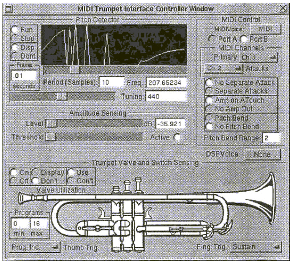
\includegraphics[width=\textwidth]{img-2-eps-converted-to-crop.pdf}
\caption{Interface panel for the Cook/Morrill Trumpet}
\label{Cook:cook-fig:1}       % Give a unique label
\end{figure}



Another project, the HIRN wind controller, sensed rotation and translation in
both hands, arm orientation, independent control with each finger, breath
pressure, and even muscle tension in the lips \cite{Cook:1992}.  Mappings from these controls
to the parameters of the WhirlWind meta-wind-instrument physical model allowed
exploration of new ``spaces'' of acoustical processes, and the HIRN also was
investigated as a controller for FM and other synthesis techniques.  Negative
lessons from the HIRN project indicated that huge control bandwidth is not
necessarily a good thing, and that attempting to build a ``super instrument''
\textit{with no specific musical composition to directly drive the project}
(\textit{principle 5}) yields interesting research questions, but with no real
product or future direction.   One positive lesson from the project is that the
\textit{co-design of synthesis/ processing algorithms with controllers} can
benefit both.

\begin{figure}[t]
\centering
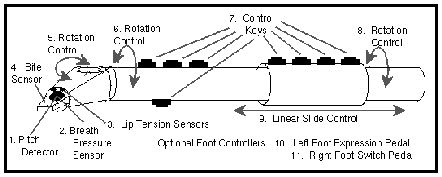
\includegraphics[width=\textwidth]{img-1-eps-converted-to-crop.pdf}
\caption{The HIRN Meta-Wind Controller}
\label{Cook:cook-fig:2}       % Give a unique label
\end{figure}


\section{Voice:  SPASM  1988--94   }

Research on physical modeling of the voice resulted in the construction of the
SPASM/Singer voice synthesizer  \cite{Cook:1991,Cook:1992a} (see Figures~\ref{Cook:cook-fig:3} and \ref{Cook:cook-fig:4}).  The SPASM system
was capable of real time synthesis, but had well over 40 continuously controlled
parameters.  Work to improve the graphical interfaces and add control via MIDI
fader boxes \cite{Cook:1993a} proved that the voice is a truly difficult ``instrument'' to
control (\textit{principles 3 \& 4}).  Recent work in real-time vocal model
control will be discussed in the SqueezeVox Section.


\begin{figure}[t]
\centering
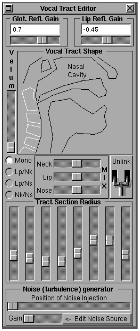
\includegraphics[height=80mm]{img-3-eps-converted-to-crop.pdf}           
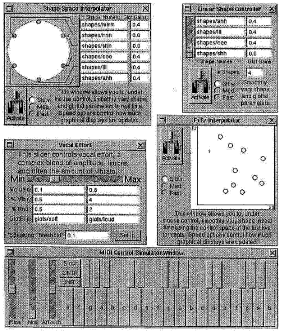
\includegraphics[height=80mm]{img-4-eps-converted-to-crop.pdf}
\caption{SPASM (left), Few-to-Many Mappings (right)}
\label{Cook:cook-fig:3}       % Give a unique label
\end{figure}



\section{PhISEM Shaker Percussion: 1996--1999}

The PhISEM (Physically Inspired Stochastic Event Modeling) project \cite{Cook:1996,Cook:1997} provided support for the ``\textit{new algorithms lead to new controllers lead to new algorithms \ldots{}}'' principles.  This work on the synthesis of particle-type percussion and real-world sounds led to a set of new instruments, not only for control of shaker/scraper sounds and sound effects, but also for algorithmic interactive music.  For example, the Frog Maraca (Figure~\ref{Cook:cook-fig:4}) sends MIDI commands to control a simple algorithmic fusion jazz combo of bass, piano, and drums.  The success with both adults and children of the Frog Maraca at Agora98 European children’s television workshop, Cyprus, Greece, came from its simple interface (just shake it), the fun of making fairly complicated music with such a simple and whimsical looking device, and the fact that it only performed one function (and always performed that function when turned on).  A related shaker percussion instrument controller was a Tambourine that could also compose algorithmic modal marimba solos when shaken.

\begin{figure}[t]
\centering
%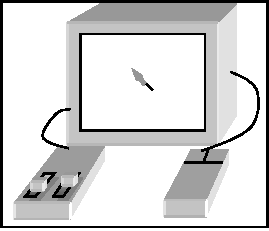
\includegraphics[width=78mm]{img-5-eps-converted-to-crop.pdf}
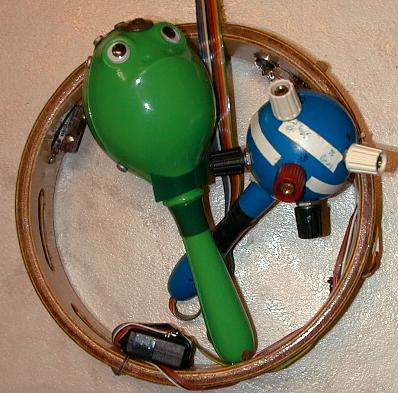
\includegraphics[width=78mm]{Figure5PhiSEM.jpg}
\caption{PhISEM controllers}
\label{Cook:cook-fig:4}       % Give a unique label
\end{figure}


Constructing the PhISEM controllers provided rich evidence that ``\textit{Programmability is a curse},'' and a correlary: ``\textit{Smart instruments are often not smart}.''  What these principles are meant to address is that the programmability of computer-based musical systems often make them too easy to configure, redefine, remap, etc.  For programmers and composers, this provides an infinite landscape for experimentation, creativity, writing papers, wasting time, and never actually completing any art projects or compositions. For normal humans, being able to pick up an instrument with a simple obvious interaction and ``play it'' only makes logical sense.  That the instrument is ``learning from their play and modifying its behavior'' often does not make any sense at all, and can be frustrating, paralyzing, or offensive.  PhISEM controllers have a single embedded microcontroller, programmed for one or two functions (selectable by the state of a button on power-up), and they put out standard General \textit{MIDI} signals.  Except for the need to replace batteries (\textit{Die Batteries Die!!}), these controllers have a strong possibility of working perfectly as designed in 10 (perhaps 20) years.  Those who craft complex systems using custom hardware, multiple computers, and multiple operating systems, can make no such claims.

\section{Foot, Hand, Kitchen Wear/Ware  1997--2000}

Spurred by the success of the PhISEM controllers, the notion of simple, MIDI
based, fixed single function controllers was continued, but based on objects that
are not specifically associated with music.  Figure~\ref{Cook:cook-fig:6} shows the TapShoe,
constructed at Interval Research as part of Bob Adams' Expressions Project.  This
shoe used force sensing resistors and accelerometers attached directly to a DSP
board running PhISEM shaker algorithms and a small rhythmic loop.  The algorithm
generated a basic ``groove'' to which the wearer of the shoe could add accents
and dynamics, in addition to their own tapping sounds.  The success of the system
came from giving the TapShoe wearer that feeling that they were actually
performing the music, though the algorithmic loop would play a relatively boring
tapping sound even if the shoe sat unworn (``\textit{Instant music, subtlety
later}'').

The Pico Glove (see Figure~\ref{Cook:cook-fig:5}) was \textit{designed as a single composition},
called ``Pico I for Seashells and Interactive Glove'' \cite{Cook:1997a}.  The idiomatic
gesture of moving the hand in and out of the shells was enhanced by a tilt sensor
in the glove.  This was used to steer fractal note-generation algorithms in real
time, to accompany the blown shells.

\begin{figure}[t]
\centering
%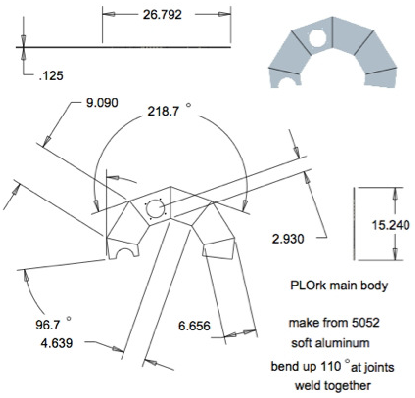
\includegraphics[width=48mm]{img-6-eps-converted-to-crop.pdf}   
%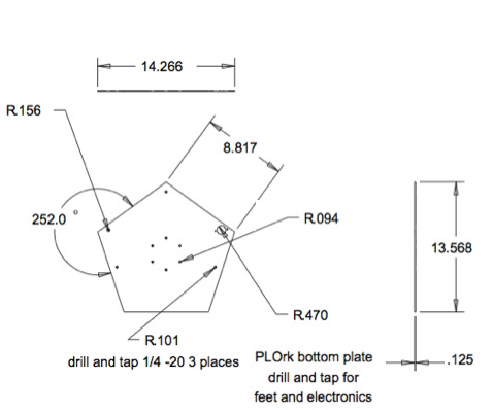
\includegraphics[width=48mm]{img-7-eps-converted-to-crop.pdf}
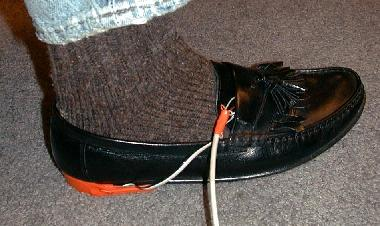
\includegraphics[height=35mm]{Figure6TapShoe.jpg}   
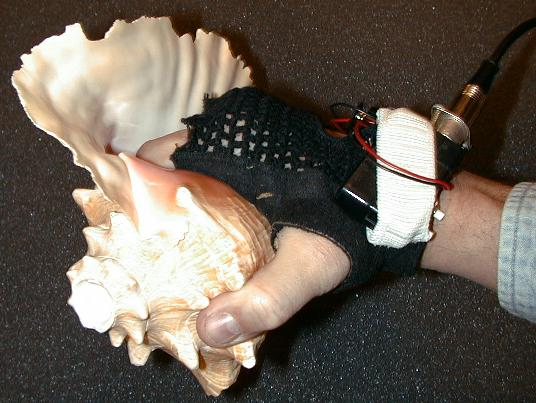
\includegraphics[height=35mm]{Figure7PicoGlov2.jpg}
\caption{Digital Tapshoe (left), PicoGlove (right)}
\label{Cook:cook-fig:5}       % Give a unique label
\end{figure}



The JavaMug (Figure~\ref{Cook:cook-fig:6}) was designed for a transcontinental MIDI jam session held
in 1997 between Tokyo and Columbia University \cite{Goto:1997}.  Being one of the author's
favorite objects, the coffee mug fits comfortably into the hand, and pressure
sensors beneath the fingers, a tilt sensor, a pot and two buttons allow control
of an algorithmic techno-latin band.   The principle of ``\textit{Instant music,
subtlety later}'' is dominant in this instrument.  Simply picking up the JavaMug
and squeezing it yields attractive and (fairly) deterministic music, because
algorithmic randomness is increased by \textit{decreasing} pressure on the
sensors.  After playing the instrument for a while, neophytes grow to more expert
levels by realizing that the music gets more varied and interesting if they
experiment with the relative pressures and tilts.  Note that this is also an
example of the ``\textit{Smart instruments are often not smart}'' principle, in
that the instrument doesn't change at all, but rather trains the user to use more
gentle and subtle manipulations of the sensors.  Other kitchen-related interfaces
include the ``Fillup Glass,'' which plays minimalist music loops (\textit{via
MIDI}) controlled by sensors in a water glass, and ``P-Ray's Caf\'{e}: Table 1''
which allows the control of a melodic percussion group by movement of common
table-top items (sugar, salt shaker, etc) over the surface of a small table. 
These objects showed that ``\textit{Everyday objects suggest amusing
controllers.}''

\begin{figure}[t]
\centering
%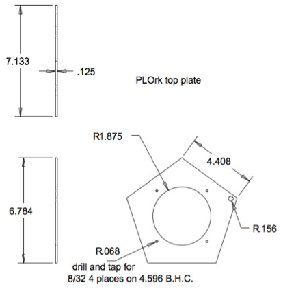
\includegraphics[width=78mm]{img-8-eps-converted-to-crop.pdf}
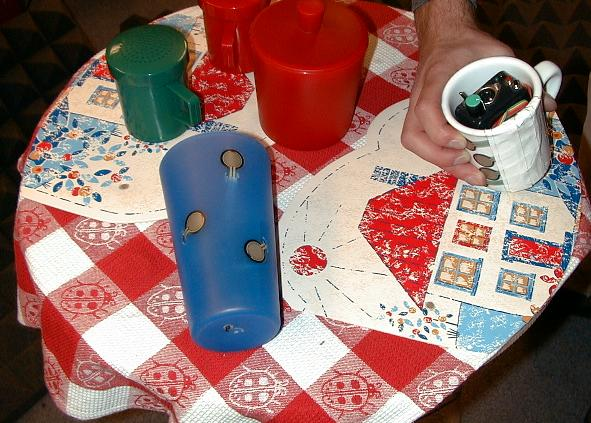
\includegraphics[width=\textwidth]{Figure8P-RaysCafe.jpg}
\caption{P-Ray's Caf\'{e}, with Fillup Glass and Java Mug}
\label{Cook:cook-fig:6}       % Give a unique label
\end{figure}


\section{Violins/Strings:  BoSSA, the Nukelele    1998--99}

Stringed instruments have a rich historical musical tradition.  They also have a
rich tradition of electronic interfaces, both commercially and experimentally
with many electrified, MIDI, and pure digital violins and guitars.  Work with Dan
Trueman at Princeton University began with a sensor-enhanced violin bow called
the ``RBow,'' and the NBody project which worked to study and model the
directional radiation properties of stringed instruments \cite{Cook:1999}.  Dan continued and
expanded this work, yielding BoSSA (The Bowed Sensor, Speaker Array, Figure~\ref{Cook:cook-fig:7})
 \cite{Trueman:1999}.  Lessons learned and reinforced by the BoSSA project include
``\textit{Existing instruments suggest new controllers},'' and ``\textit{Copying
an instrument is dumb, leveraging expert technique is smart}.'' Other principles
reinforced are ``\textit{Some players have spare bandwidth, some do not},''
(violin players generally have their hands completely occupied, so a successful
interface must exploit interesting remappings of existing gestures),  and
``\textit{Wires are not that bad (compared to wireless)}'' (the BoSSA is played
sitting by a player who often plays electric violin, so the increased complexity
of wireless was not justified).

The Nukelele (thanks to Michael Brooke for the name) was constructed in Bob
Adams' Interval Research Expressions project.  While collaborating on other
Expressions projects such as ``the Stick'' and the `` Porkophone,'' the Nukelele
was a personal experiment to design, implement, and test a new controller as
rapidly as possible.  The Nukelele was intended to match the expressiveness of a
true stringed instrument, by using audio directly from a sensor to drive a
plucked string physical model.  Two sandwiched linear force sensing resistors
under the right hand served to provide pluck/strike position information, along
with the audio excitation for the string model.

\begin{figure}[t]
\centering
%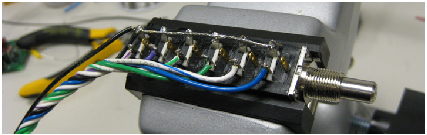
\includegraphics[width=48mm]{img-9-eps-converted-to-crop.pdf}  
%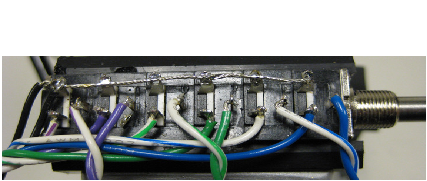
\includegraphics[width=48mm]{img-10-eps-converted-to-crop.pdf}
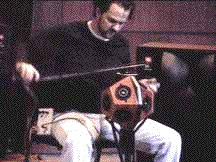
\includegraphics[height=35mm]{Figure9BoSSA.jpg}  
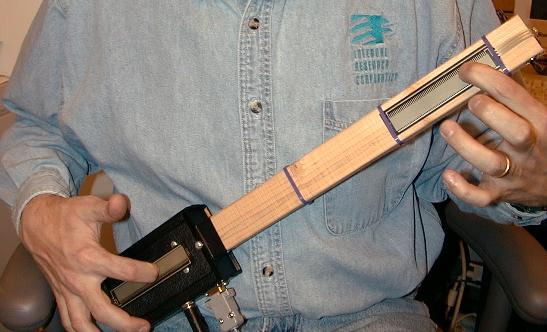
\includegraphics[height=35mm]{Figure10Nukelele.jpg}
\caption{BoSSA (left), the Nukelele (right)}
\label{Cook:cook-fig:7}       % Give a unique label
\end{figure}


\section{The Voice (again): SqueezeVox    2000}

The SqueezeVox project \cite{Cook:2000} a suitable controller for models of the human voice. 
Breathing, pitch, and articulation of vowels and consonants must be controlled in
a vocal model, so  the accordion was selected as a natural interface
(\textit{principle 10}).  Pitch via the keyboard, vibrato aftertouch, and a
linear strip for fine pitch and vibrato are controlled with the right hand. 
Breathing is controlled by the bellows, and the left hand controls vowels and
consonants via buttons (presets), or continuous controllers such as a touch pad,
plungers, or squeeze interface.

\begin{figure}[t]
\centering
%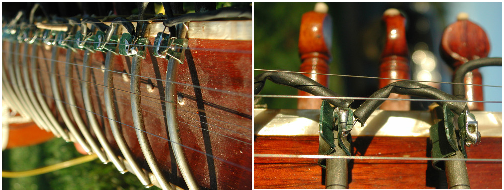
\includegraphics[width=48mm]{img-11-eps-converted-to-crop.pdf}      
%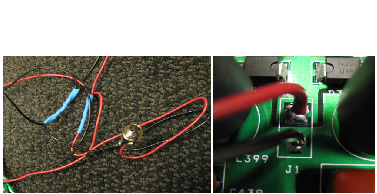
\includegraphics[width=48mm]{img-12-eps-converted-to-crop.pdf}
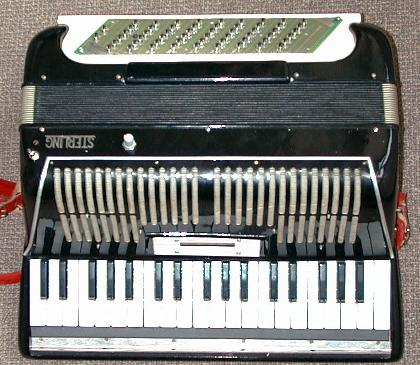
\includegraphics[height=40mm]{Figure11SQBart.jpg}      
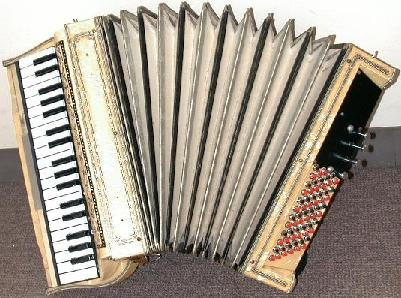
\includegraphics[height=40mm]{Figure11SQLisa.jpg}
\caption{Squeezevox Lisa (left) and Bart (right)}
\label{Cook:cook-fig:8}       % Give a unique label
\end{figure}



\section{Future Work  and Conclusions}

Work and development continues on the SqueezeVox project, with a self-contained
version (Santa's Little Helper, with onboard DSP synthesis), and a small
concertina version (Maggie) currently under construction.  Work also continues on
the kitchen/common objects project, and given the variety of such objects, much
rich interface and music design lies ahead.

Musical interface construction proceeds as more art than science, and possibly
this is the only way that it can be done.  Yet many of the design principles put
forth in this paper have held true in multiple projects, and many have been
verified in talking with other digital instrument designers.  Some of the
technological issues might go away, but not completely or not necessarily very
quickly.  Many of the human/artistic issues are likely to be with us as long as
musical instruments have been.

\section{Demonstrations}

During the workshop, the PhISEM controllers, the JavaMug, the TapShoe, the
Nukelele, and the SqueezeVox will be demonstrated.  Soundfiles, large pictures,
% Origintal text:
%and video clips of the instruments discussed in this paper are available at: 
%\href{http://www.cs.princeton.edu/~prc/CHI01.html}{http://www.cs.princeton.edu/~prc/CHI01.html}
% edited to: 
and video clips of the instruments discussed in this paper are available online.\footnote{\url{http://www.cs.princeton.edu/~prc/CHI01.html}}

\begin{acknowledgement}
Specific thanks to Dexter Morrill, Dan Trueman, Bob Adams, and Colby Leider. 
General thanks to all those at CCRMA, Princeton, and Interval Research for
wonderful collaborations.  This work was funded by CCRMA and the CCRMA Industrial
Affiliates Program, Interval Research, Intel, and the Arial Foundation.
\end{acknowledgement}



\section*{Author Commentary: NIME: 15 years later. Wow!}

\paragraph{Perry Cook}


What a run it's been.  I could never have imagined that this paper might become one of my most cited and downloaded publications, but I guess it makes sense for a variety of reasons.  Here I ponder some of those reasons, and give some thoughts on the time since.

First, it was the very first NIME, actually the ACM/CHI workshop, before the NIME organization and conference itself began running autonomous from ACM CHI.  So the network effect of being one of the first papers helps a lot.

I won't pretend that the information in this paper was particularly sage or epic by any means, but it did provide a good introductory reader and reference for a new curriculum area just getting started in music tech programs around the world.  Long before NIME (5 or 10 years or more before) there were courses like Dan O'Sullivan's Physical Computing course at ITP/NYU, and some other HCI Technology courses (like the multi-university San Jose State + CCRMA + Princeton + others course that Ben Knapp and Dick Duda \cite{Knapp:1995} got started with many of us back in 1996).  But with the birth of NIME, courses like this could be re-focussed on music (the true goal for many of us all along), so having a NIME course made sense for many music technology and digital arts curricula.

This paper came before a lot of other cool things that happened in my academic and artistic life.  Most of the experiences that brought about my 2001 list of NIME Principles came from working with NIME builders: at CCRMA, and with DanO, Bob Adams, Michael Brook, Geoff Smith, Dan Levitin, Bill Verplank, and others at Interval Research \cite{Levitin:2002}, and Ben Knapp and others on our own HCI Technology courses \cite{Knapp:1995}.  Princeton and my DSP+NIME curriculum brought me Dan Trueman and BoSSA, Ge Wang and ChucK, many (hemi)spherical speakers with Dan, Scott Smallwood, Curtis Bahn, Stephan Moore and others, the Princeton Laptop Orchestra (and many other LORks), Ajay Kapur and his Karmetik Robots and Machine Orchestra, Rebecca and Wekinator, many other great students, and lots of other NIME developments.

Finally, I updated the paper subsequently with new insights, revisions, and corrections based on changing technology or a different vantage point on my part.

My NIME 2007 Keynote at NYU, titled: ``Principles for Controlling Computer Music Designers,'' \cite{Cook:2007} took a look at teaching a NIME curriculum, and early lessons from the Princeton Laptop Orchestra.  So I added some new principles:  

\begin{enumerate}
 \setcounter{enumi}{14}
	\item More can be better (but hard) (PLORk went from an initial 15 members,  to 35!)
	\item Music+Science is a great teaching/marketing tool (important in academic jobs)
	\item The younger the student, the more fearless (they don't know/care what's hard)
\end{enumerate}

My NIME 2009 paper, ``Re-Designing Principles for Computer Music Controllers: a Case Study of SqueezeVox Maggie,'' \cite{Cook:2009} was about revisiting some older versions of my NIME instruments and my experiences with actually re-designing/re-building them.  And of course, I changed one: 

\begin{enumerate}
 \setcounter{enumi}{12}
	\item (b) Funny is often much better than serious (whimsical designs are not a crime)
\end{enumerate}

\noindent
and added even more new principles:

\begin{enumerate}
 \setcounter{enumi}{17}
\item Redesign for backward compatibility (make sure you can play your old pieces)
\item Design (and pack) for post-9/11 travel (document, make sure things demo easily)
\item (a) Build a (new) copy, don't trash the original (keep it around to compare), and (b) Build two or more if you can afford it. (one will invariably work better)
\item Wire and document for future surgeries  (labeled 20 in paper, should be 21)
\item Build in diagnostic features and displays (labeled 21, should be 22)  
\item Construct controller proxies (functional GUIs) (labeled 22, should be 23)
\end{enumerate}

So one additional (personal) principle that I would add has to do with double-checking the numbering of lists in papers and sequels.  Another principle might be that we never know where a piece of work, or publication, or small workshop as an adjunct to a larger conference, might lead.  The ACM/CHI New Interfaces for Musical Expression workshop turned into something bigger than any of us might have dreamed.

I'm really happy to have been a part of the NIME history (so far).  All indications are that we've still got a lot ahead of us.


\section*{Expert Commentary: Perry Cook's Principles Still Going Strong}

%\paragraph{Marcelo M. Wanderley, McGill University, marcelo.wanderley@mcgill.ca}
\paragraph{Marcelo M. Wanderley}

The NIME 2001 workshop was a very interesting venue. A rather active musical controllers community already existed for several years in 2001—mostly active at the International Computer Music Conference (ICMC), with key papers in the area already published before the NIME workshop (including many by Perry himself. See the electronic book ``Trends in Gestural Control of Music'' for a state of the art in 2000).\footnote{\url{http://www.idmil.org/projects/trends}} Even so, the NIME 2001 workshop was a unique opportunity to meet researchers directly working in this area, see demos of their work at the Experience Music Project in Seattle, and discuss possible ways to organize a research community around it. Several of the papers presented in the workshop became main references in our field, with several hundred citations each: Perry's, Wessel and Wright's \cite{Wessel:2001} and Orio et al.'s \cite{Orio:2001}, the two last ones with sequels published in the 2002 Computer Music Journal special edition (vol. 26, number 3) on NIME.

It was very interesting to re-read Perry Cook's 2001 NIME workshop paper, as well as its NIME 2009 follow up paper where he reviews the original 2001 guidelines in light of newer developments. Perry's 2001 paper belongs to a tradition of works from builders/performers (or performer/builders) who excel in both areas. Such works have the advantage of bringing to the community lots of personal, first hand performance experience informed by a strong technical/scientific component. In this sense, it is complementary to works by designers who mostly focus on technical aspects, who nevertheless collaborate with (multiple) artists when designing their devices. The advantage of the later group is that one can (hopefully!) more easily avoid one's own aesthetic ideas about music and art and provide a larger, albeit forcefully less coherent, set of examples from which to derive guidelines. The study of both approaches, taking into consideration their own strengths and limitations, should lead to interesting (and informed!) designs. 


It is amazing to see that in almost 15 years, many (most?) of its principles and guidelines still hold true. My favorites are (\#4) ``Some players have spare bandwidth, some do not'' (true, how true!), (\#2) ``Smart instruments are often not smart,'' (\#1) ``Programmability is a curse,'' and (\#6) ``Instant music, subtlety later.'' The last one ties well to Wessel and Wright's principle: ``Low entry fee, with no ceiling on virtuosity'' \cite{Wessel:2001}.


Being part of the group who focuses mostly on technical issues (an example of a great paper about design is \cite{Bongers:2000}), I am less in agreement with principle \#5 (``Make a piece, not an instrument or controller''), as I have seen many interesting instruments made without a musical piece in mind, but that subsequently were extensively used musically. The case in mind is Joe Malloch's t-Stick \cite{Malloch:2007}, who in collaboration with composer/performer D. Andrew Stewart, developed a device that became an established instrument used in dozens of musical pieces (check Andrew's impressive t-stick performance videos at vimeo.com). 

I also take principles \#10 and \#11 (``New algorithms suggest new controllers'' and ``New controllers suggest new algorithms'') with a grain of salt, as I believe that they underplay the idea importance of mapping (between controller outputs and algorithm inputs). Complex mapping strategies can provide tools to use a variety of algorithms with the same controller (e.g. \cite{Hunt:2002}), leading to interesting instruments. Furthermore, not all instrument designers are proficient in sound design and might just want to use algorithms they are familiar with, even when using different controllers (and conversely).

Finally, other principles seem to have become less useful with time, as for instance, battery life that has dramatically improved in the last 15 years (\#8), making the use of cables is less necessary in instrument design (although still useful in many occasions!) (\#9). In short, this is still a very useful, inspiring paper. Perry's direct style is excellent and the review of his previous works until then is enlightening. Some of its principles will hold for a long time (forever?) and have become basic bricks to our community. 



\graphicspath{ {mainmatter/Wessel_2001/} }

\title*{2001: Problems and Prospects for Intimate Musical Control of Computers}
\titlerunning{Intimate Musical Control of Computers}



\author{David Wessel and Matthew Wright}
\authorrunning{Wessel and Wright}


%\institute{David Wessel \at Center  for New Music and Audio Technologies Department of Music, University of California, Berkeley, California 94720 USA, \email{wessel@cnmat.berkeley.edu} \and Matthew Wright \at  Center  for New Music and Audio Technologies Department of Music, University of California, Berkeley, California 94720 USA, \email{matt@cnmat.berkeley.edu}}
%
%
\maketitle

\abstract*{In this paper we describe our efforts towards the development of live performance computer-based musical instrumentation. Our design criteria include initial ease of use coupled with a long term potential for virtuosity, minimal and low variance latency, and clear and simple strategies for programming the relationship between gesture and musical result. We present custom controllers and unique adaptations of standard gestural interfaces, a programmable connectivity processor, a communications protocol called Open Sound Control (OSC), and a variety of metaphors for musical control. We further describe applications of our technology to a variety of real musical performances and directions for future research.}

\section{Introduction}

When asked what musical instrument they play, there are not many computer music practitioners who would respond spontaneously with ``I play the computer.'' Why not? In this report we examine the problems associated with the notion of the computer as musical instrument and the prospects for their solution.

Here at the onset it would be useful to consider some of the special features that computer technology brings to musical instrumentation. Most traditional acoustic instruments such as strings, woodwinds, brass, and percussion place the performer in direct contract with the physical sound production mechanism. Strings are plucked or bowed, tubes are blown, and surfaces are struck. Here the performer's gesture plays a direct role in exciting the acoustic mechanism. With the piano and organ the connection between gesture and sound is mediated by a mechanical linkage and in some modern organs by an electrical connection. But the relation between the gesture and the acoustic event remains pretty much in what one might call a \textit{one gesture to one acoustic event} paradigm.

When sensors are used to capture gestures and a computing element is used to generate the sound, a staggering range of possibilities become available. Sadly but understandably, the electronic music instrument industry with its insistence on standard keyboard controllers maintains the traditional paradigm. Musical instruments and their gestural interfaces make their way into common use or not for a variety of reasons most of which are social in character. These more sociological aspects like the development or not of a repertoire for the instrument are beyond the scope of this paper. Here we will concentrate on factors such as ease of use, potential for development of skill, reactive behavior, and coherence of the cognitive model for control.

In Figure~\ref{Wessel:img-2} we provide a conceptual framework for our controller research and development. Our human performer has intentions to produce a certain musical result. These intentions are communicated to the body's sensorimotor system (``motor program''). Parameters are sensed from the body at the gestural interface. These parameters are then passed to controller software that conditions, tracks, and maps them to the algorithms that generate the musical material. Admittedly this diagram is schematic and incomplete. One aspect that is not well captured by it is the way in which performers' intentions are elaborated upon by discovery of new possibilities afforded by the instrument. Experimental and otherwise exploratory intentions are certainly dear to the authors. We find that this albeit schematic framework allows us to view the roles of human motor learning, controller mapping, and generative software as an overall adaptive system \cite{Lee:1992}.

\begin{figure}[t]
\centering
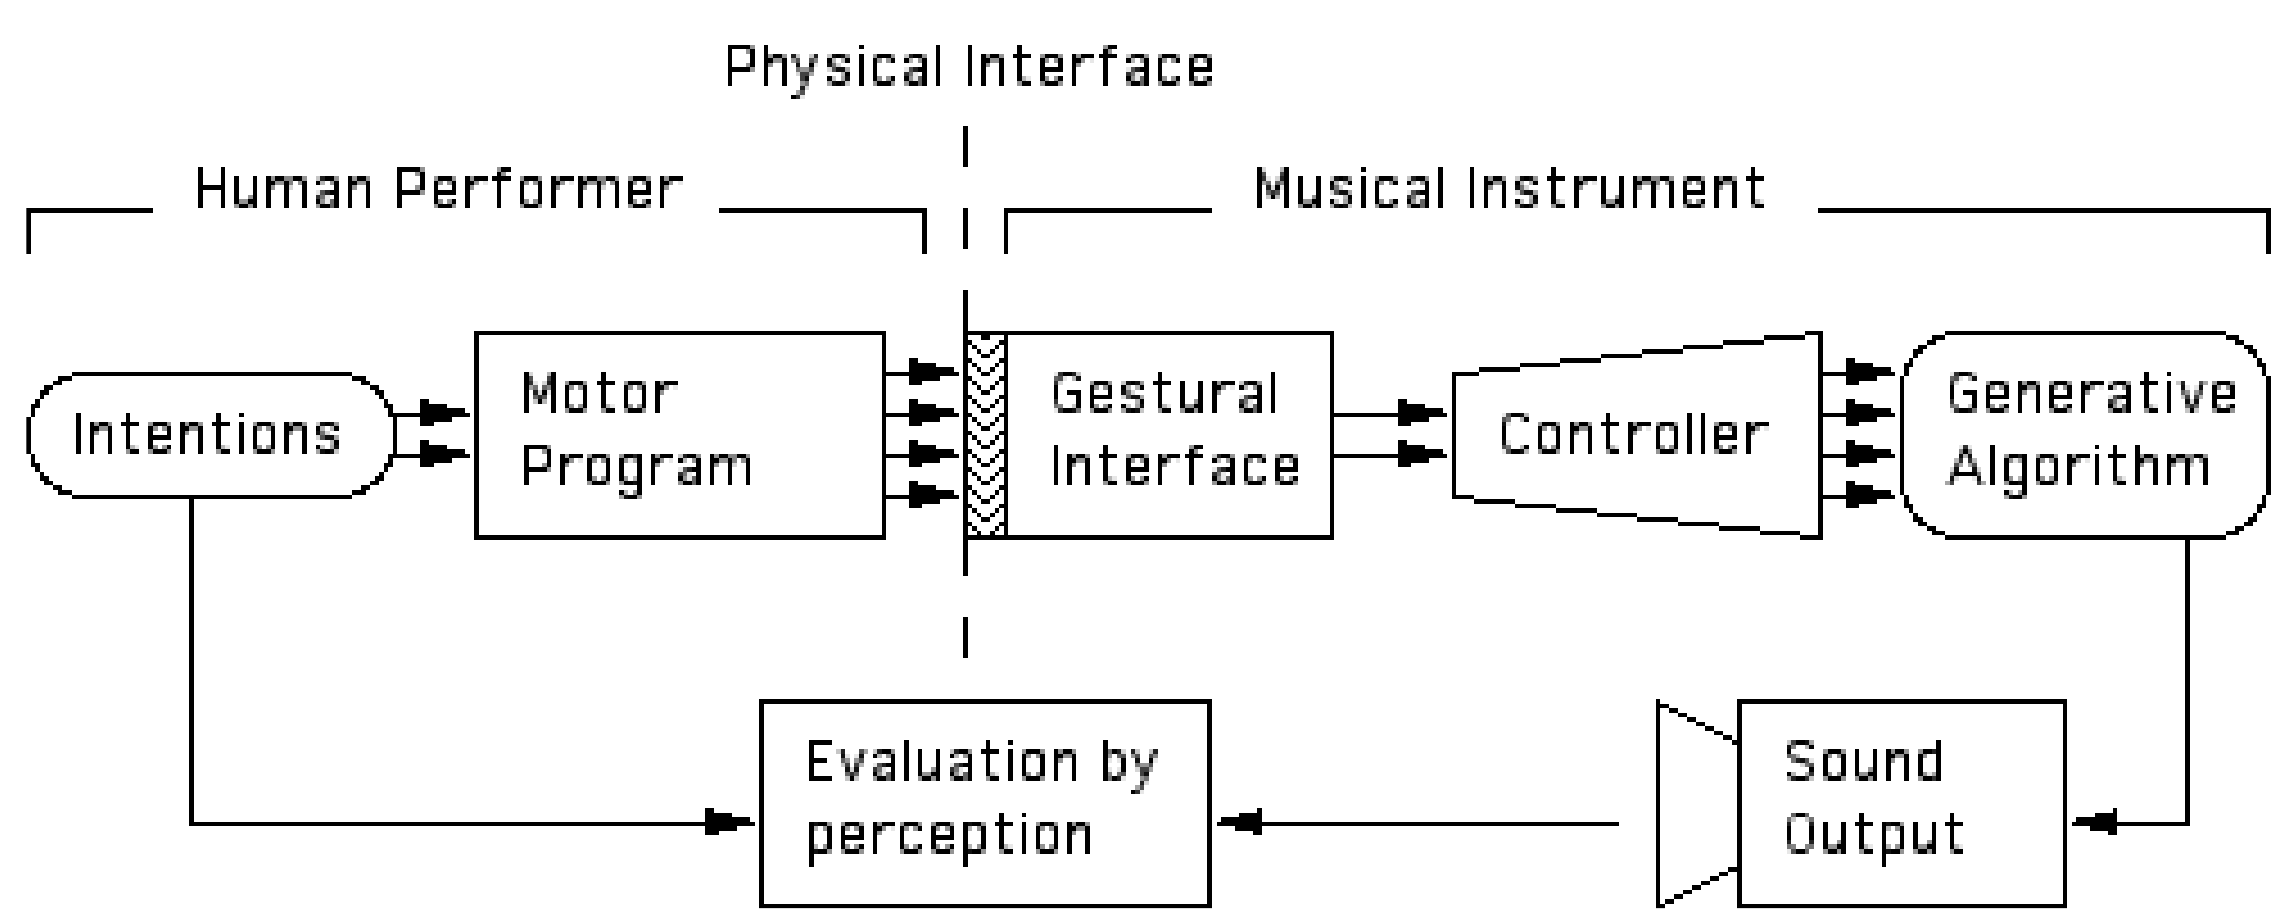
\includegraphics[width=\textwidth]{wessel_fig1.png}
\caption{Conceptual framework for NIME research and development.}
\label{Wessel:img-2}
\end{figure}

Unlike the \textit{one gesture to one acoustic event} paradigm our framework allows for generative algorithms to produce complex musical structures consisting of many events. One of our central metaphors for musical control is that of \textit{driving} or \textit{flying} about in a space of musical processes. Gestures move through time as do the musical processes.

\section{Low entry fee with no ceiling on virtuosity}

Getting started with a computer-based instrument should be relatively easy but this early stage ease-of-use should not stand in the way of the continued development of musical expressivity. Most of the traditional acoustical musical instruments are not easy to play at first but do afford the development of a high degree of musicality. On the other hand many of the simple-to-use computer interfaces proposed for musical control seem, after even a brief period of use, to have a toy-like character and do not invite continued musical evolution.

Is the low entry fee with no ceiling on virtuosity an impossible dream? We think not and argue that a high degree of control intimacy can be attained with compelling control metaphors, reactive low latency variance systems, and proper treatment of gestures that are continuous functions of time. With the potential for control intimacy assured by the instrument, musicians will be much more inclined to the continued development of performance skill and personal style.

\section{Latency requirements for control intimacy}

Few practitioners of live performance computer music would deny that low latency is essential. Just how low is the subject of considerable debate. We place the acceptable upper bound on the computer's audible reaction to gesture at 10 milliseconds (ms) and the systems described in this paper provide for measured \cite{Freed:1997} latencies nearer 7 ms.

Low variation of latency is critical and we argue that the range of variation should not exceed 1 ms. Grace-note- generated timbres as in flams can be controlled by percussionists with temporal precision of less than 1 ms. This is accomplished by controlling the relative distance of the sticks from head during the stroke. Timbral changes in the flams begin to become audible when the variations in the time between the grace note and the primary note exceed 1 ms. Psychoacoustic experiments on temporal auditory acuity provide striking evidence for this criterion \cite{Henning:1981,Ronken:1970}. As we will argue below, prospects for the solution to the latency variation problem can be resolved by using time tags or by treating gestures as continuous signals tightly synchronized with the audio I/O stream.

\section{Discrete Event Versus Continuous Control}

MIDI is a discrete event protocol. MIDI events turn notes on and off and update changes in controller values. MIDI events are almost never synchronized with digital audio samples. Furthermore, MIDI provides no mechanism for atomic updates. Chords are always arpeggios and even when MIDI events are time tagged at the input of a synthesizer they arrive as a sequence. Moore \cite{Moore:1988}, McMillen \cite{McMillen:1994}, and Wright \cite{Wright:1994} provide numerous examples of the dysfunction of MIDI. Much of this dysfunction is addressed by the Open Sound Control (OSC) protocol described below.

Many musical gestures are continuous functions of time and should be treated as such, for example, the position along the string of a finger on a violinist's left hand. The new generation of software synthesis systems such as Max/MSP, SuperCollider, PD, and Open Sound World (OSW) provide for multi-rate signal processing. In these programming environments it is quite natural to treat gestures with a sample-synchronous signal processing approach. CNMAT's connectivity processor \cite{Freed:2000b} described below provides a mechanism for getting continuous gestures into the computer in a manner that is very tightly synchronized with the audio sample stream. With this system we demonstrate a significant increase in control intimacy.

\section{Open Sound Control (OSC)}

Open Sound Control is a discrete event protocol for communication among controllers, computers, sound synthesizers, and other multimedia devices that is optimized for modern networking technology. Entities within a system are addressed individually by an open- ended URL-style symbolic naming scheme that includes a powerful pattern matching language to specify multiple recipients of a single message. We provide high- resolution time tags and a mechanism for specifying groups of messages whose effects are to occur simultaneously. Time tags allow one to implement a scheduling discipline \cite{Dannenberg:1989} that reduces jitter by trading it for latency.

OSC's use of symbolic names simplifies controller mapping and its hierarchical name space helps in the management of complexity. There is also a mechanism for dynamically querying an OSC system to find out its capabilities and documentation of its features. OSC has been integrated into Max/MSP (by Matthew Wright), Csound (by Stefan Kersten and Nicola Bernardini) SuperCollider (by James McCartney), and OSW (by Amar Chaudhury). It has been used in a variety of contexts involving controllers.\footnote{See \url{http://www.cnmat.berkeley.edu/OSC} for more detail and downloadable OSC software.}

\section{A Programmable Connectivity Processor}

The conventional approach for communicating gesture and sound to real-time performance systems is to combine a microcontroller or DSP chip with A/D, D/A convertors and a network interface such as a MIDI serial controller. We have developed an alternative, more flexible approach that supports scalable implementations from a few channels of audio and gestures to hundreds of channels.

Our new system to address computer music and audio connectivity problems is based on integrating all digital functions on a single field programmable gate array (FPGA). All functions are determined by compiling high- level hardware descriptions (in VHDL) into FPGA configurations. This approach allows the considerable investment in developing the interface logic to each peripheral to be easily leveraged on a wide variety of FPGA's from different vendors and of different sizes. Since FPGA's are now available in sizes greater than a million gates, entire DSP and microcontrollers can also be integrated if required.

We have developed and tested VHDL descriptions for processing serial audio data for the SSI, S/PDIF, AES/EBU, AES-3, and ADAT industry standards. For gestures that are continuous we sample at submultiples of the audio rate and have VHDL modules for multichannel 8-bit, 12-bit and 16-bit A/D converters. We also provide modules for multiple MIDI input and output streams. Although such descriptions have been developed forproprietary systems, this library of modules represents the first complete, independent suite available in VHDL.

This suite makes possible some unusual cross codings such as embedding gestural data in audio streams, increasing temporal precision by exploiting isochronous data paths in the control processor. We sample continuous gestural signals at a submultiple of the audio sampling rate, multiplex the channels, and represent them as audio input signals. This allows us to get gestural signals into our software with the same low latencies as audio input, and guarantees that gestural and audio input signals will be tightly synchronized.

A novel module of particular importance in portable computer-music performance systems implements fast Ethernet from the hardware layer up through IP to the UDP protocol of TCP/IP. Because of the importance of Internet performance, Fast Ethernet implementations are extremely reliable and finely tuned on all modern operating systems.

A key feature of the connectivity processor is the analog subsystem for continuous gesture acquisition. We currently provide for 32 channels of analog-to-digital conversion. Voltage ranges of the converters are selectable as are the sampling rates which are constrained to be integer divisions of the audio rate and the appropriate antialiasing filter cutoff frequencies.

Our system combines VHDL connectivity modules that multiplexes 8 channels of bidirectional audio, MIDI, S/PDIF and transduced gestures into UDP packets which are exchanged with a portable computer using new, customized ASIO drivers in Max/MSP \cite{Avizienis:2000}.
% This link is dead, citing paper instead.
%\footnote{See www.cnmat.berkeley.edu/ICMC2000 for a more detailed description of CNMAT's connectivity processor.}


\section{Musical Control Structures for Standard Gestural Controllers}

Throughout history, people have adapted whatever objects were in their environment into musical instruments. The computer industry has invested significant resources in creating broadly available, low cost gestural controllers without any musical application in mind; thoughtful adaptation of these controllers for music is a fruitful yet overlooked route.

We find the latest incarnations of the venerable digitizing tablet (a.k.a. ``artist's tablet'') very interesting for musical control. Tablets offer accurate and fast absolute position sensing of cordless devices in three dimensions. Additionally, pressure, orientation, tilt and rotation estimates are available. The tablet we use allows for simultaneous sensing of two devices, usually one in each hand. This rich, multidimensional control information can be mapped to musical parameters in a variety of interesting ways.

The most direct kind of mapping associates a single synthesis parameter with each control dimension, for example, vertical position controlling loudness, horizontal position controlling pitch, etc. This kind of mapping proved to be musically unsatisfying, exhibiting the toy-like characteristic that does not allow for the development of virtuosity.

More interesting interfaces define regions of the tablet associated with particular behaviors. For example, one region might consist of a grid providing access to a large palette of musical material, while other regions represent musical processes that can operate on selected musical material. Repeating rhythmic cycles can be represented graphically on a region of the tablet, and sonic events can be placed at particular time points within the cycle \cite{Wright:1998}.

We have created software in the Max/MSP environment that we use to develop control structures for the two- handed digitizing tablet. Examples include navigation in timbre space, multidimensional synthesis control, note stream synthesis, and emulations of the gestures of strumming, plucking and bowing strings. We also developed an interactive musical installation that uses two joystick controllers.

\section{Some Custom Controllers}

At CNMAT we have developed applications for variety of custom controllers, these include Don Buchla's Thunder and Lightning,\footnote{\url{http://www.buchla.com}} Tactex controllers,\footnote{\url{http://www.tactex.com}} Force Sensing Resistor (FSR) technology \cite{Rovan:1997}, and Piezo electric sensors in conjunction with percussion \cite{Campion:1999}. We currently have research projects underway that exploit a key feature of the previously described connectivity processor---namely the synchronization of control signals with the audio I/O stream. These projects include an organ keyboard with continuous sensing of each key position \cite{Freed:2000}, a variety of micro-accelerometer projects, and new FSR devices.

In addition we have developed new sensor systems for multidimensional string motion \cite{Freed:2000a} and have made some advances in extracting control signals from vocal sounds.

\section{Metaphors for Musical Control}

As suggested in the introduction, metaphors for control are central to our research agenda. We have found the work of George Lakoff and his collaborators \cite{Lakoff:1999,Lakoff:2000} on embodied cognition to be particularly applicable. They argue that abstract concepts like time and space and even the loftier concepts of mathematics are grounded in sensorimotor experience. We now present some of the metaphors that have inspired the development of our controller software.

\section{Drag and Drop}

The drag and drop metaphor is well known to users of the Apple Macintosh. An object is selected picked up and dropped upon a process. This is a natural application of Lakoff's movement and container metaphors. Our drag and drop system has been extended to the problem of the control of musical processes using the pen and tablet interface. Musical material is selected and then dropped onto a musical process.

One of the most critical features of any musical control system is a silencer, a mechanism that allows the performer to gracefully shut down a musical process. To this end we have the performer place the pen on theprocess and using a circular motion like the traditional copy editor's cursive delete sign the process is silenced at a rhythmically appropriate point in time. Other interfaces use the ``eraser'' end of the pen to silence processes.

\section{Scrubbing and its Variants}

Sinusoidal models allow arbitrary time-scale manipulation without any change in pitch or spectral shape. We have built ``scrubbing'' interfaces for the tablet in which one dimension of the pen's position on the tablet maps to the time index of a sinusoidal model. Moving the pen gradually from left to right at the appropriate rate results in a resynthesis with the original temporal behavior, but any other gesture results in an alteration of the original. This interface allows a performer to play more arbitrary musical material, while preserving the fine continuous structure of the original input sounds. This kind of interface has been used in live performance contexts with classical Indo-Pakistani singing \cite{Wessel:1998}, trombone samples with expressive glissandi, and saxophone quartet material.

Other dimensions of the tablet sensing data, e.g., pressure, tilt, and vertical position, can be mapped to synthesis parameters such as loudness and spectral shape.

\section{Dipping}

In the ``dipping'' metaphor the computer constantly generates musical material via a musical process, but this material is silent by default. The performer controls the volume of each process, e.g., using a poly-point touch- sensitive interface with the pressure in each region mapped to the volume of a corresponding process. Other gestural parameters control other parameters of the musical processes.

An advantage of this metaphor is that each musical event can be precisely timed, regardless of the latency or jitter of the gestural interface. Once a given process is made audible, its rhythm is not dependent on the performer in an event-by-event way.

This kind of interface is most satisfying when there are multiple simultaneous musical processes of different timbres, allowing the performer to orchestrate the result in real-time by selecting which processes will be heard.


\begin{acknowledgement}
Special thanks to Rimas Avizienis, Adrian Freed, and Takahiko Suzuki for their work on the connectivity processor and to Gibson Guitar, DIMI, and the France Berkeley Fund for their generous support.
\end{acknowledgement}




\section*{Unsolved Problems and Continuing Prospects for Intimate Musical Control of Computers}

\paragraph{Matthew Wright}


When we wrote this article in 2001 (and expanded it into a fuller article the following year \cite{Wessel:2002}) there seemed to be a small community of people making music interactively with computer-based instruments of their own design, and as far as I could tell all of them were friends with David Wessel.  We jumped on the opportunity to share our thoughts on goals, difficulties, and techniques for achieving a quality of intimacy that we strongly desired in our own instruments and found lacking in most of the triggering-based instruments then readily available.  We were excited that the esteemed ACM SIGCHI was to some degree turning its attention to questions of musical interaction, and welcomed the opportunity to shape this discussion by injecting our own values and methods.  We had no idea this small fringe gathering would develop into the NIME conference and community as it now exists.

Today I question the relationship between NIME and mainstream CHI.  Although computer music has always benefitted from and indeed depended on advances in EE and computer science generally not made with music in mind, it does not seem that the concerns of NIME have had much influence on CHI in particular. In the other direction, much of the apparent influence of CHI on NIME has been shoehorning the inherently creative and exploratory artistic process of designing musical instruments into the objectively quantifiable mindset of evaluating task performance. Today the minimum viable NIME paper seems to be a slightly novel combination of technologies that is demonstrably good at something, with only the best making theoretical contributions to guide the exploration of the infinite-dimensional space of possible instruments with ethical consideration of the potential of the human performer.   Perhaps if we could better capture and theorize the experiences of skilled practitioners as contributions to knowledge, themes of performance, expertise, experience, artistry, and control could become more prominent to the betterment of both communities.  

Low entry fee with no ceiling on virtuosity, aka Low Floor High Ceiling (a phrase popularized by Seymour Papert that reached us via Brian Harvey), is perhaps the most-cited idea in this paper, though of course it is much easier to demonstrate the floor than the ceiling.  We disparaged low-ceiling NIMEs as ``toy-like;'' I now regret this phrase and prefer to frame the question as how to design high-ceiling toys.  Toys and their enclosing adaptive systems can harm or help the continued musical evolution of kids of all ages, inviting and rewarding human motor learning in many ways.  Gurevich et al. rightly question the importance of an instrument's inherent properties in light of people's seemingly inexhaustible creativity in adapting their music making to even the simplest of NIMEs \cite{Gurevich:2010}.  Nevertheless, I would still argue that their beeping button box's and other excellent toys' remarkably high ceilings (e.g., variety) can be predicted and partially attributed to low latency/jitter and a drive to apply continuous control even to an instrument that presents a discrete-only interface.

Latency raises the floor and jitter lowers the ceiling; indeed these have been a major theme of NIME, questions that are today almost required of proposed NIMEs and their component technologies.  A few papers focus exclusively on these issues.  We arrived at our 10 +/- 1 ms criterion through subjective personal experiences using instruments with various measured latencies and our flam timbre justification through thought experiment; to my knowledge the literature still lacks better empirical justification for these engineering constraints.  In the context of graphical objects following a user's finger on a touch screen, 1ms total latency is clearly\footnote{The demonstration video \url{http://www.youtube.com/watch?v=vOvQCPLkPt4} is compelling.} much better than 10ms \cite{Jota:2013}. Perceptual and cognitive studies of various musical activities and results under various latency/jitter conditions could also result in better models for how skilled performers adapt and possibly shed light on development of musicality in general.

Wessel's SLABS\footnote{\url{http://cnmat.berkeley.edu/user/david_wessel/blog/2009/01/15/slabs_arrays_pressure_sensitive_touch_pads}} represent the fullest embodiment of this paper's goals and ideas, with extremely low latency, OSC (whose huge impact on the NIME community is addressed in Chapter~\ref{chapter:Wright_2003}), a representation of gestural data as audio signals, a direct descendent of the programmable connectivity processor isochronously scanning a poly-point touch-sensitive gestural interface, and the ``dipping'' metaphor in its most satisfying form.  Many NIMEs centering on a digitizing tablet \cite{Zbyszynski:2007} have joined my continuing work, which includes recent experiments spatially arranging sound grains in 3D according to analyzed acoustical properties, then flying about this space, still a rich and powerful metaphor.  Scrubbing remains vital to my tablet interfaces, but the analysis portion of sinusoidal modeling is still difficult and likely to produce unsatisfactory results without extensive fussing, hampering widespread adoption of this technique.   Granular scrubbing seems more promising, with the high dimensional control space of window size, rate, etc both a challenge and opportunity. 

Understandably, the number of cases of developing a deep, longstanding, and fruitful connection to a NIME is far less than the number of NIMEs that have been proposed.  One could argue that modular synthesis' current popularity, with many performers developing intimate relationships with their personal instruments, is because they ``treat gestures with a sample-synchronous signal processing approach;'' unfortunately it is still very common for NIMEs to sample or delay control signals much more slowly and erratically, to our detriment.  I would like to see and perform additional research into these control signals (e.g., their spectral and phase properties) in sophisticated musical contexts.



\section*{The Sempiternal Quest for Intimacy}

\paragraph{Sergi Jord\`{a}}

2001 was the year the first NIME took place. A small workshop inside the huge CHI conference in Seattle, I was lucky enough to be one of the first dozen NIME participants ever. There, I had the honor to meet some of the pioneers and gurus of the burgeoning ``live computer music world'' (for the lack of a better term, ``NIME'' not yet existing before the workshop): Max Mathews, Bill Verplank, Perry Cook, Joe Paradiso … were all there, giving presentations that would enlighten and guide the younger ones such as myself. If I remember correctly, David Wessel did not attend the workshop---I would have to wait one or two more years for meeting him in person and becoming good friends---and Matt Wright gave their presentation.

Wessel and Wright's paper introduces one of the concepts that would come to recur most frequently in our NIME community: that of ``low entry fee with no ceiling on virtuosity.'' The paper starts also with one sentence, that while less popular, still constitutes one of my favourite NIME quotes; one, which I subsequently often borrowed and even used for starting my Phd thesis: ``When asked what musical instruments they play, there are not many computer music practitioners who would respond spontaneously with \lq I play the computer.\rq ''  But the paper encompasses much more than some popular NIME quotes; it does, in fact, contain almost too much. It ranges from conceptual topics, such as control intimacy and its importance for attaining a hypothetical instrumental virtuosity, to fully technical solutions such as the OSC protocol, which had been specifically designed for addressing the low latency and the high resolution requirements previously identified by the authors as being essential for attaining the aforementioned intimate control. On top of this, it introduces some musical interfaces and controllers which were then being designed, revamped or customised at CNMAT, and it concludes with a discussion on some of the control metaphors that inspired the development of these interfaces. If that wasn't enough, some essential knowledge (then novel and original) is dropped here and there, such as the empirically observed toy-like behaviour of ``one-to-one mappings'' (although the authors do not employ that term), and their unsuitability for the development of virtuosity.

Considering its generous loquacity, it is very likely that by today's standards, a paper like this would have been rejected for publication: ``lack of clear objective and structure, and lack of evidence and proof for most of the authors' statements.'' While its overwhelming flood of ideas was tamed for the extended and matured journal version published a year later \cite{Wessel:2002}, and which probably constitutes a more cohesive reading, I would like to stress the fact that urgency to communicate and effervescence, were indeed the trademarks of most of the papers presented at this first NIME workshop in 2001. Much knowledge and know-how had been accumulated and was pressurized, eager to be shared with a sympathetic audience! But this specific paper, together with Perry Cook's ``Principles for Designing Computer Music Controllers'' \cite{Cook:2001}, which was also presented at the 2001 workshop, clearly stand as two of the early pillars or compendiums of NIME knowledge. Together with two even earlier seminal publications by Pressing \cite{Pressing:1990} and Ryan \cite{Ryan:1992}, they still constitute the first four introductory must-read papers in any NIME-related course I have ever organized!

In 2001, NIME-knowledge was necessarily based on personal experience and empiricism. This type of knowledge is not easily replicable, not always demonstrable, not very scientific in sum, but it is not less valid for these reasons. Fifteen years later, the NIME community has matured and a growing number of university courses are being taught \cite{Jorda:2014}. Yet, creating DMIs is still, in many respects, very similar to creating music. It involves a great deal and variety of know-how and technicalities, while at the same time, as in music, there are no inviolable laws.  Indeed, in his contemporary aforementioned paper \cite{Cook:2001}, Cook sceptically and romantically affirmed: ``musical interface construction proceeds as more art than science, and possibly this is the only way it can be done?'' Because I tend to agree with him, I believe we should never forget the previous successes and the failures of experienced practitioners. In that sense, it comes as no surprise that the first tentative and informal---but still very valid---NIME design and conceptual frameworks were proposed by experienced digital luthiers, performers and educators, and David Wessel, regretfully not longer with us, definitely excelled in all these categories.


\graphicspath{  {mainmatter/Hunt_2002/} }
\title*{2002: The importance of parameter mapping in electronic instrument design}
\titlerunning{Parameter Mapping in Electronic Instrument Design}

\author{Andy Hunt, Marcelo M. Wanderley and Matthew Paradis}
\authorrunning{Hunt et al.}

%\institute{Andy Hunt \at Music Technology Group, Electronics Department, University of York, Heslington, York YO10 5DD, \email {email adh2@york.ac.uk}
%\and Marcelo M. Wanderley \at Faculty of Music, McGill University 555, Sherbrooke Street West H3A 1E3---Montreal---Canada \email{mwanderley@acm.org}
%\and Matthew Paradis \at Music Technology Group, Music Department University of York, Heslington, York YO10 5DD \email{email mdjp100@york.ac.uk}}
%
%
\maketitle

\abstract*{In this paper we challenge the assumption that an electronic instrument consists
solely of an interface and a sound generator.  We emphasise the importance of the
mapping between input parameters and system parameters, and claim that this can
define the very essence of an instrument.}

\section{Electronic Instruments and the Mapping Layer}

In an acoustic instrument, the playing interface is inherently bound up with the
sound source.  A violin's string is both part of the control mechanism and the
sound generator.  Since they are inseparable, the connections between the two are
complex, subtle and determined by physical laws.  With electronic and computer
instruments, the situation is dramatically different.  The interface is usually a
completely separate piece of equipment from the sound source.  This means that
the relationship between them has to be defined.  The art of connecting these
two, traditionally inseparable, components of a real-time musical system (an art
known as \textit{mapping}) is not trivial.  Indeed this paper hopes to stress
that by altering the mapping, even keeping the interface and sound source
constant, the entire character of the instrument is changed.  Moreover, the
psychological and emotional response elicited from the performer is determined to
a great degree by the mapping.

\section{The Importance of Mapping}

In this section we emphasise the dramatic effect that the style of mapping can
have on ``bringing an interface to life.'' We focus on our own experience in
designing digital musical instruments and comment on several previous designs. An
extensive review of the available literature on mapping in computer music has
been presented by the authors in \cite{Hunt:2000b}, \cite{Wanderley:2001} and \cite{Wanderley:2002}.

\section{Informal Observations }

The first author has carried out a number of experiments into mapping.  The more
formal of these have been presented in detail in \cite{Hunt:2000} and \cite{Hunt:1999}, 
and are summarised later in this paper. Let us begin with some rather simple, yet interesting,
observations that originally sparked interest in this subject.  We have retained
the first person writing style to denote that these are informal, personal
reflections.

\subsection{The Accidental Theremin }

Several years ago I was invited to test out some final university projects in
their prototype form in the lab.  One of them was a recreation of a Theremin with
modern electronic circuitry.  What was particularly unusual about this was that a
wiring mistake by the student meant that the ``volume'' antenna only worked when
your hand was moving.  In other words the sound was only heard when there was a
rate-of-change of position, rather than the traditional position-only control. 
It was unexpectedly exciting to play.  The volume hand needed to keep moving back
and forth, rather like bowing an invisible violin.  I noted the effect that this
had on myself and the other impromptu players in the room.  Because of the need
to keep moving, it felt as if your own energy was directly responsible for the
sound.  When you stopped, it stopped.  The subtleties of the bowing movement gave
a complex texture to the amplitude.  We were ``hooked.''  It took rather a long
time to prise each person away from the instrument, as it was so engaging.  I
returned in a week's time and noted the irony that the ``mistake'' had been
corrected, deleted from the student's notes, and the traditional form of the
instrument implemented.

\subsection{Two Sliders and Two Sound Parameters }

The above observation caused me to think about the psychological effect on the
human player of ``engagement'' with an instrument.
To investigate this further I constructed a simple experiment. The interface for
this experiment consisted of two sliders on a MIDI module, and the sound source
was a single oscillator with amplitude and frequency controls.  In the first run
of the experiment the mapping was simply one-to-one, i.e. one slider directly
controlled the volume, and the other directly controlled the pitch (cf. Figure~\ref{Hunt:img-6}).

\begin{figure}[t]
\centering
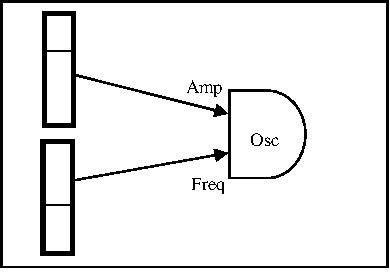
\includegraphics[width=70mm]{img-6-eps-converted-to-crop.pdf}
\caption{Simple mapping for Experiment 1}
\label{Hunt:img-6}       % Give a unique label
\end{figure}

I let several test subjects freely play with the instrument, and talked to them
afterwards.  In the second experimental run, the interface was re-configured to
emulate the abovementioned ``accidental Theremin.''  One slider needed to be moved
in order to make sound; the rate of change of movement controlled the
oscillator's amplitude.  But I decided to complicate matters (on purpose!) to
study the effect that this had on the users.  The pitch, which was mainly
controlled by the first slider, operated ``upside-down'' to most people's
expectations (i.e. pushing the slider up lowered the pitch).  In addition the
second slider (being moved for amplitude control) was used to mildly offset the
pitch---i.e. it was cross-coupled to the first slider  (cf. Figure~\ref{Hunt:img-2}).


\begin{figure}[t]
\centering
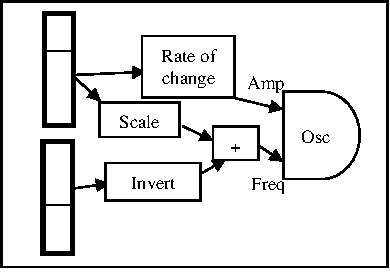
\includegraphics[width=70mm]{img-2-eps-converted-to-crop.pdf}
\caption{Complex mapping for Experiment 2}
\label{Hunt:img-2}       % Give a unique label
\end{figure}


A remarkable consistency of reaction was noted over the six volunteers who tried
both configurations.  With Experiment 1, they all commented within seconds that
they had discovered how the instrument worked (almost like giving it a mental
``tick''; ``yes, this is volume, and this is pitch'').  They half-heartedly tried to
play something for a maximum of two minutes, before declaring that they had
``finished.''  Problem solved.

With Experiment 2, again there was a noted consistency of response.  At first
there were grumbles.  ``What on earth is this doing?''  ``Hey---this is affecting
the pitch''  (implied cries of ``unfair,'' ``foul play'').  But they all struggled
with it---interestingly for several more minutes than the total time they spent
on Experiment 1.   After a while, their bodies started to move, as they developed
ways of offsetting one slider against the other, while wobbling the first to
shape the volume.  Nearly all the subjects noted that somehow this was rewarding;
it was ``like an instrument.''  Yet in both cases the interface (two sliders) and
the sound source (a single oscillator) were identical.  Only the mapping was
altered, and this had a psychological effect on the players.

\section{Mapping Experiments}

Several formal investigations have been carried out by the authors in order to
explore the essence and the effect of this mysterious mapping layer.

\subsection{Complex Mapping for Arbitrary Interfaces}

The first author carried out an investigation into the psychology and practicality of various interfaces for real-time musical performance \cite{Hunt:1999}.  The main part of this study took the form of major series of experiments to determine the effect that interface configuration had on the quality and accuracy of a human player's performance.  The details of the theory, experiments and results have been published \cite{Hunt:2000}.  They are summarised here, in order to give an overview of their implications for mapping strategies.

Three interfaces were used, and these are now described. The first interface (cf. Figure~\ref{Hunt:img-3}) represented a typical computer music editing interface with on-screen sliders connected one-to-one to each sound parameter. The second (cf. Figure~\ref{Hunt:img-4}) involved physical sliders (on a MIDI module) again connected in a one-to-one manner to the synthesis unit. The third interface (cf. Figure~\ref{Hunt:img-5}) consisted of a series of multi-parametric cross-mappings, and---like the accidental Theremin mentioned above---required constant movement from the user to produce sound.


\begin{figure}[t]
\centering
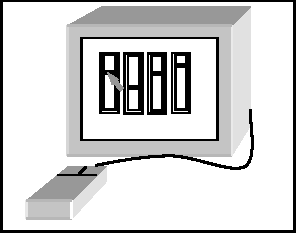
\includegraphics[width=70mm]{img-3-eps-converted-to-crop.pdf}
\caption{The ``mouse'' interface}
\label{Hunt:img-3}       % Give a unique label
\end{figure}



\begin{figure}[t]
\centering
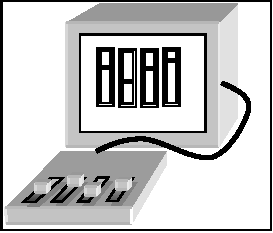
\includegraphics[width=70mm]{img-4-eps-converted-to-crop.pdf}
\caption{The ``sliders'' interface}
\label{Hunt:img-4}       % Give a unique label
\end{figure}



\begin{figure}[t]
\centering
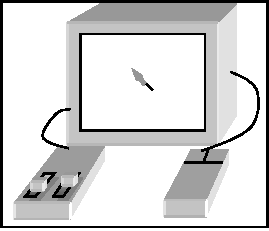
\includegraphics[width=70mm]{img-5-eps-converted-to-crop.pdf}
\caption{The `multi-parametric' interface}
\label{Hunt:img-5}       % Give a unique label
\end{figure}


Users attempted to copy (using each interface) a series of sounds produced by the computer.  The accuracy of reproduction was recorded for each user, over several attempts, spread out over a number of weeks.  Results were gathered numerically, and plotted on a series of graphs to compare the effect---over time---of each interface.  These quantitative results can be summarised for the multiparametric interface as follows:

\begin{itemize}
	\item The test scores in general were much higher than those for the other two
interfaces, for all but the simplest tests.
	\item There was a good improvement over time across all test complexities.
	\item The scores got better for more complex tests!
\end{itemize}

This last result may seem rather counter-intuitive at first sight; that people
performed better on the harder tasks.  However, this brings into question the
definition of a `hard task.'  If an interface allows the simultaneous control of
many parameters, maybe it really is easier to perform the more complex tasks, and
harder to accurately isolate individual parameters.

A range of qualitative results was also gathered by interviewing the test
subjects to establish their subjective experience of using each interface.  They
all concluded that the ``mouse'' interface was the most limited---as they could see
how impossible it would be to operate more than one parameter simultaneously. 
Surprisingly perhaps, they were nearly all extremely frustrated and angered by
the 4 physical sliders.  Comments abounded such as ``I should be able to do this,
technically, but I can't get my mind to split down the sound into these 4 finger
controls.''  Some users actually got quite angry with the interface and with
themselves.  The multi-parametric interface, on the other hand, was warmly
received---but not at the very beginning.  At first it seemed counter-intuitive
to most users, but they rapidly warmed to the fact that they could use complex
gestural motions to control several simultaneous parameters without having to
``de-code'' them into individual streams.  Many users remarked how ``like an
instrument'' it was, or ``how expressive'' they felt they could be with it.

\subsection{Focusing on the Effect of Mapping Strategies}

In the above experiment several factors may have affected the results.  For
instance, the multiparametric interface used cross-coupled parameters in addition
to the user's energy. It also decreased reliance on visual feedback, and provided
two-handed input, all of which may have contributed in varying degrees to the
interface's effectiveness.  An additional experiment was subsequently carried out
by the third author to focus entirely on the user's reaction to a change in
mapping strategy.

These tests utilised three contrasting mapping strategies, with a fixed user
interface and synthesis algorithm. The mappings were;

\begin{enumerate}
	\item simple one-to-one connections between input and output,

	\item one-to-one requiring the user's energy as an input.  This was implemented by
requiring the user to constantly move one of the sliders in a ``bowing''-like
action

	\item many-to-many connections from input to output, but also requiring the user's 
energy as in b).

\end{enumerate}

These mappings were used to control the parameters of a stereo FM synthesis
algorithm, including amplitude, frequency, panning, modulation ratio and
modulation index. The input device used was a MIDI fader box.  Users were asked
to play with each interface until they felt they had a good sense of how to
`drive it' to perform musical gestures.  No time limit was given to this process;
the users were encouraged to explore the possibilities of each set-up.  Data was
collected on the users' (subjective) views on the comparative expressivity and
learnability of each mapping and the accuracy of musical control that could be
achieved.

Whilst experimenting with the first mapping test (one-to-one) many users noted
that the simple division of parameters was not very stimulating. Users tended to
learn the parameter associations very quickly but then struggle to achieve any
improvement in their performance or expressive output.

The second test generated a range of comments, which suggested that the process
of injecting energy into a system presented a much more natural and engaging
instrument.  However, due to the proximity of sliders on the interface they found
it difficult to control other sliders whilst providing the required ``bowing''
action.  However, this problem lessened over time as the user practised.

The third and final user test (many-to-many mappings) provided some interesting
results.  Most of the test subjects noted that the appeal of this instrument was
that it was not instantly mastered but required effort to achieve satisfactory
results.  The instrument presented a challenge to the user, as one would expect
from a traditional expressive instrument.

These tests highlighted the differences between a general-purpose interface,
(such as the mouse) which has simple mappings but allows the user to begin
working instantly, and an interface with more complex mappings which must be
practised and explored in order to achieve truly expressive output.

\subsection{Learning from Acoustic Instruments}

In \cite{Rovan:1997} the second author and collaborators discussed the fact that by altering
the mapping layer in a digital musical instrument and keeping the interface (an
off-the-shelf MIDI controller) and sound source unchanged, the essential quality
of the instrument is changed regarding its control and expressive capabilities.

Previous studies, notably by Buxton \cite{Buxton:1986}, presented evidence that input devices
with similar characteristics (e.g. number of degrees of freedom) could lead to
very different application situations depending on the way these characteristics
were arranged in the device. In that study, however, the devices were not exactly
the same mechanically (one had two separate controllers and the other one
two-dimensional controller), so the situation is not the same as when using the
same input device with different mapping strategies, even if the results are
similar.

In \cite{Rovan:1997}, a Yamaha WX7 wind controller was used as the input device, and sound
was generated using additive synthesis models of clarinet sounds in IRCAM's FTS
environment (later in jMax).

The idea behind the project was simple: many wind instrument performers
complained that MIDI wind controllers tend to lack expressive potential when
compared to acoustic instruments such as the clarinet or saxophone.  A common
path to solving this problem involves improving the design of the controller by
adding extra sensors.  However, it was decided to challenge this assumption and
to solely work on the mapping layer between the controller variables and the
synthesis inputs (for a complete description see \cite{Rovan:1997}).

Another point became clear in this process: even if the WX7 was a faithful model
of a saxophone providing the same types of control variables (breath, lip
pressure and fingering), these variables worked totally \textit{independently} in
the MIDI controller, whereas they are \textit{cross-coupled} in acoustic
single-reed instruments. This natural cross-coupling is the result of the
physical behaviour of the reed, and since the equivalent ``reed'' in the
controller was a plastic piece that did not vibrate, and moreover was not coupled
to an air column, variables were simply independent.

Based on these decisions and facts, the authors proposed different mappings
between the WX7 variables and the synthesis parameters.  The first was basically
a one-to-one relationship, where variables were independent.  The second was a
model where the ``virtual airflow'' through the reed (loudness) was a function of
both the breath and lip pressure (embouchure), such as in an acoustic instrument.
 The third was a model that took into account both the ``virtual airflow'' and
the relationship between spectrum content to breath and embouchure; a model that
would match even more closely the real behaviour of the acoustic instrument.

Using these three different models, the system was performed by different
musicians and non-musicians. Results indicated that wind instrument performers
tended to stick with complex cross-coupled mappings similar to the single reed
behaviour (the third mapping strategy used), whereas beginners initially
preferred simpler mappings (easier to play and produce stable sounds).


\begin{figure}[t]
\centering
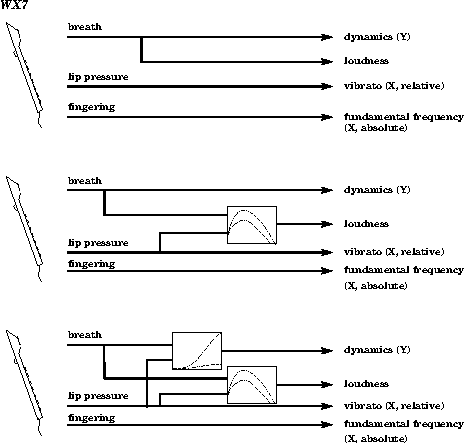
\includegraphics[width=\textwidth]{img-1-eps-converted-to-crop.pdf}
\caption{Several mappings used in the clarinet simulation presented in
 \cite{Rovan:1997}.}
\label{Hunt:img-1}       % Give a unique label
\end{figure}


The two most important consequences of this work were:

\begin{itemize}
	\item By just changing the mapping layer between the controller and the synthesis
algorithm, it was indeed possible to completely change the instrumental behaviour
and thus the instrument's feel to the performer. Depending on the performer's
previous experience and expectations, different mappings were preferred.

\item By deconstructing the way that the reed actually works, it was noted that the
choice of mapping could be important as a pedagogical variable. Indeed, in stark
contrast with acoustic instruments where the dependencies between parameters are
unchangeable, cross-coupling between variables can easily be created or destroyed
in digital musical instruments. This means that performers could focus on
specific aspects of the instrument by explicitly defining its behaviour. Possible
options could include:

\begin{itemize}
	\item complex (cross-coupled) control of loudness with one-to-one control of timbre,
	\item one-to-one loudness and complex timbre controls, or,
	\item complex loudness and timbre controls, such as in the real instrument.
\end{itemize}

\end{itemize}


Even if these results supported the essential role of mapping (and the
importance of devising mapping strategies other than one-to-one during the design
of digital musical instruments), they could not be easily extrapolated to more
general situations. In fact, in the above specific case, there \textit{did exist}
a model of complex mapping to be followed, since the controller was a model of
the acoustic instrument. So what about mappings in general digital musical
instruments using alternate controllers, those not based on traditional acoustic
instruments?

\section{Models and Guidelines For Mapping}

Since there will not always be ready models for inspiration when designing
mapping strategies for new digital musical instruments, the task then becomes one
of proposing guidelines for mapping and also, if possible, devising models that
can facilitate the implementation of mapping strategies other than simple
one-to-one relationships.

In trying to answer this question of how to extend a specific mapping solution
to a more general case, a model of mapping for digital musical instruments was
proposed in \cite{Wanderley:1998}.  It was based on the separation of the mapping layer into two
independent layers, coupled by an intermediate set of user-defined (or
``abstract'') parameters. This model was presented in the framework of a set of
extensions to jMax later known as ESCHER (actually, a set of objects developed by
Norbert Schnell to perform interpolation using additive models).

This idea is based on previous works, such as those of Mulder et al. \cite{Mulder:1997},
M\'{e}tois \cite{Metois:1996}, and Wessel \cite{Wessel:1979}. A similar direction was presented by Mulder and
Fels in \cite{Mulder:1998a} and later by Garnett and Goudeseune \cite{Garnett:1999}. Basically, all these works
have used higher levels of abstraction as control structures instead of raw
synthesis variables such as amplitudes, frequencies and phases of sinusoidal
sound partials. The main point made in \cite{Wanderley:1998} was to explicitly think about two
separate mapping layers and the strategies to implement these, and not on the
choice of intermediate parameters themselves, whether perceptive, geometrical or
``abstract'' \cite{Wanderley:1999}.

The intrinsic advantage of this model is its flexibility. Indeed, for the same
set of intermediate parameters and synthesis variables, the second
mapping layer is independent of the choice of controller being used. The same
would be true in the other sense: for the same controller and the same set of
parameters, multiple synthesis techniques could be used by just adapting
the second mapping layer, the first being held constant. Specifically in this
case, the choice of synthesis algorithm is transparent for the user

The original two-layered model has recently been expanded to include three
mapping layers in two independent performance works by Hunt and Myatt (RIMM The Real-time Interactive MultiMedia project, and
by Arfib and collaborators \cite{Arfib:2002}.  These works support the idea that, by using
multi-layered mappings, one can obtain a level of flexibility in the design of
instruments and that moreover, these models can indeed accommodate the control of
different media, such as sound and video, in a coherent way.

\subsection{One-to-one Mappings---Multiple Layers}

We have noted that there is a tendency for designers to make one-to-one mappings
when constructing an interface.  We can \textit{use} this tendency to improve the
mapping process if we utilise the many layered models outlined above.  The
following scenario may illustrate this:

Imagine a system whose interface inputs included `button 1,' `button 2,'  `slider
1,' `slider 2,' `mouse x,' and `mouse y.'  Let us suppose that the synthesis system
was a Frequency Modulation module with inputs such as `carrier frequency,'
`carrier amplitude,' `modulation frequency' etc.  Now consider the two
possibilities below:

	
\begin{description}
\item[Case 1:] let us consider a designer working to connect the above inputs
to the above outputs.  We are quite likely to see arbitrary connections such as 
``mouse x controls carrier frequency,'' and ``slider 1 controls modulation
frequency.''  These give us the oft-encountered one-to-one mappings.

\item[Case 2:] let us imagine that a mapping layer has already been devised to
abstract the inputs to parameters such as `energy,' `distance between sliders,'
`wobble' etc.  Also let us imagine that there is a mapping layer before the FM
synthesis unit, providing higher-level control inputs such as `brightness,'
`pitch,' `sharpness' etc.  Now we can picture the designer making a relationship
such as ``energy controls brightness.''  On the surface this may appear to be yet
another one-to-one mapping.  Indeed it is---at the conceptual level. 
However, when you consider how `energy' is calculated from the given inputs, and
how `brightness' has to be converted into the FM synthesis primitives, you will
notice how many of the lower-level parameters have been cross-coupled.

\end{description}


Thus the many-level mapping models are a way of simplifying the design process,
and of helping the designer to focus on the final effect of the mapping, as well
as providing a convenient method of substituting input device or synthesis
method.

\section{Future Discussion of Mapping}

From the evidence presented above in both informal and controlled experiments,
there is definitely a need to come up with better-designed mappings than simple
(engineering style) one-to-one relationships. General models of mappings have
been proposed and expanded to incorporate multimedia control, but also to fit
several levels of performance, from beginners to highly skilled players.

One attempt to foster the discussion in this direction has been initiated in the
context of the ICMA/EMF Working Group on Interactive Systems and Instrument
Design in Music. % \cite{:2000b}. 
A further effort is currently being carried out in the form
of a special issue on ``Mapping Strategies for Real-time Computer Music''
guest-edited by the second author \cite{Wanderley:2002} to appear as volume 7, number 2 of the
journal Organised Sound later this year.

We therefore welcome comments and criticism on issues related to mapping so as
to push the discussion on this essential---although often ignored---topic.

\section{Conclusions}

The mapping `layer' has never needed to be addressed directly before, as it has
been inherently present in acoustic instruments courtesy of natural physical
phenomena.  Now that we have the ability to design instruments with separable
controllers and sound sources, we need to explicitly design the connection
between the two.  This is turning out to be a non-trivial task.

We are in the early stages of understanding the complexities of how the mapping
layer affects the perception (and the playability) of an electronic instrument by
its performer.  What we know is that it is a very important layer, and one that
must not be overlooked by the designers of new instruments.



\section*{Author Commentary: Reflections on Parameter Mapping in Electronic Instrument Design}

\paragraph{Andy Hunt and Marcelo M. Wanderley}


In the 80's and early 90's many papers were published on the development of digital musical instruments (DMIs) and interfaces for musical expression, mostly at conferences such as the International Computer Music Conference (ICMC) and in the Computer Music Journal, both starting in the mid-late 70s. A number of amazing instruments and methods were proposed, many of them subsequently summarized in the book ``New Digital Musical Instruments: Control and interaction beyond the keyboard'' \cite{Miranda:2006}. These papers mostly presented novel interfaces and/or sound synthesis methods for musical control, but few specifically
addressed the issues involved in how to map interface outputs to synthesis inputs. One-to-one arbitrary mappings were the norm, but notable exceptions included the works of Ian Bowler et al. (ICMC1990), Michael Lee and David Wessel (ICMC1992), Insook Choi et al. (ICMC1995), Stuart Favilla (ICMC1996) and Axel Mulder et al. (Workshop Kansei 1997).

This NIME 2002 paper arose from a collaboration between Andy Hunt and Marcelo Wanderley (with Matthew Paradis, a D.Phil. student of Hunt) in the late 90's and early 2000's. Both researchers were among the first to study and begin to formalize the role of mapping in digital musical instruments (DMIs). In this paper, the questions we tackle are as follows: What if more complex strategies are used instead of one-to-one mappings, such as what happens in many acoustic musical instruments? How can one make sense of the various mapping possibilities in DMIs (e.g. implicit, explicit)? What is the influence of the choice of mapping on DMI design/performance?


Wanderley started to look at the importance of mapping in DMI design in 1997, when in collaboration with Butch Rovan, Shlomo Dubnov and Philippe Depalle he presented a paper at the International Workshop on ``Kansei, The Technology of Emotion,'' organized by Antonio Camurri in Genoa, Italy. In 1998, in collaboration with Norbert Schnell and Butch Rovan, he published a sequence paper on mapping strategies in the software application ``Escher,'' developed at IRCAM. In this paper, the notion of mapping layers was proposed to formalize and articulate the definition of mapping strategies.


At the same time, Hunt was working on his D.Phil. thesis also on mapping, under the supervision of Ross Kirk at the University of York, UK. His work was the first (and up to now possibly the only one) to have looked at the long-term performance with different mapping strategies. Apart from this major contribution, the main difference between these works was that, while Wanderley et al. were inspired by a known mapping model (that of a clarinet), Hunt and Kirk dealt with arbitrary mapping choices (i.e. with no known models to base the mapping on).


In 1999, through the project CUIDAD, organized by IRCAM and with the participation of the University of York, both had the opportunity to collaborate in joining their respective work on mapping. A first result was a paper published at ICMC 2000 in Berlin \cite{Hunt:2000b}. They continued to work on this topic through a few more papers, including the one in NIME 2002. One for Organised Sound and one for the Journal of New Music Research, directly derived from the NIME 2002 paper. Altogether, these papers were cited more than 500 times (Google Scholar, Sept 28 2015).


One interesting issue arose at the conference, held at the former Media Lab Europe, in Dublin, Ireland. One of the keynote speakers was interactive music pioneer Joel Chadabe, who gave a talk with the title ``The Limitations of Mapping as a Structural Descriptive in Electronic Instruments,'' a very interesting contrast to the title we proposed (``The importance of Parameter Mapping in Electronic Instrument Design''). This is mostly due to the notion of an ``electronic instrument,'' a reactive device in Hunt and Wanderley's view, but an ``interactive system'' in Chadabe's (see Bert Bongers definition of interactive and reactive systems \cite{Bongers:2000}).

Since then, Wanderley has edited (or co-edited) two special journal editions on Mapping in DMIs (Organised Sound vol. 7, 2002, and recently in the Computer Music Journal, vol. 38, 2014, with Joseph Malloch) and published a few more works focusing on mapping. Hunt has created and made several contributions to the field of ``interactive sonification,'' mostly in collaboration with Thomas Hermann (University of Bielefeld).

While much has been done since the paper was first written, mapping is still an open field of research,  mostly in terms of tools to help define mapping strategies in DMIs (see \cite{Wanderley:2014} for updated information). Work is still needed to understand the implications of mapping choices in short and long-term performance with DMIs.


\section*{Expert Commentary: Listen to the Inner Complexities}

\paragraph{Doug Van Nort}

Fairly early in the development of interactive computer music, people had already been thinking about user manipulation of all facets of digital sound, with a major early voice in this area being David Wessel through his idea of timbre space as a musical control structure \cite{Wessel:1979}. By the late 90's and early 2000's, ever-increasing processing speeds had allowed for high-quality sound synthesis to run in real-time. This led to an explosion in research on input devices and sensor technologies for expressive control of these various sound creation algorithms, moving beyond the limiting standard of the MIDI keyboard. 

As research raced forward in the areas of real-time sound synthesis and sensor-based controllers, a group of researchers rightly recognized that all of the essential algorithmic decisions that associate control input with sound output---the area of mapping---was being overlooked. They looked towards the more mature field of Human Computer Interaction (HCI) for inspiration, and the work of researchers such as William Buxton in order to more fully understand the ergonomic and psychological influence that simply changing a mapping can have on a user, or in this case performer. 

The article by Hunt, Wanderley and Paradis is particularly important as it represents the coming together of two early research streams. Hunt's and Wanderley's respective dissertation projects and subsequent research are two of the earliest to tackle this area of inquiry, as is well represented in the ``Trends in Gestural Control of Music'' collection \cite{:2000c} as well as a special issue of Organised Sound \cite{Wanderley:2002}. 

This NIME 2002 article serves two key purposes: the first is that it gives an important brief introduction to these preceding projects; the second is that it attempts to establish and articulate the importance of mapping by formally exploring this through quantitative and qualitative user studies. While one could level a fair criticism by noting that the studies presented lack the depth and methodological rigor of many found within the world of HCI, the fact remains that this work opened up the question of how the ostensibly simple act of control-to-sound parameter associations could profoundly impact the ``feel'' of the digital musical instrument. Various works have followed up on this early research including my own dissertation \cite{Van-Nort:2010}, largely devoted to expanding this conversation on the topic of mapping. 

Certainly not all members of the NIME community have agreed with the approach of the 2002 Hunt et al. work: some maintain that mapping is purely an artistic decision of the composer/designer, while others maintain the spirit of this article, that it is an essential determinant of expressivity for any performer who comes into contact with a given digital musical instrument. My personal view is that, as with most things, the truth lies somewhere in between and both are correct depending on the musical intent. If we are talking about a complex interactive system that a performer is simply guiding, then perhaps mapping is even a limiting concept, as proposed by Chadabe \cite{Chadabe:2002}. However, if we are talking about the continuous shaping of sonic activity with a goal of achieving nuanced control and expression that rivals acoustic instrumental practice, then this question of ``what to map where'' and how various control signals are extracted, gated, associated, adapted, conditioned, etc. can have profound impact on a digital performer's ability to keep up with their analog musical vision. 

This article has played no small role in opening up this conversation in the context of the NIME community. As we move forward with ever more sophisticated techniques of machine learning at our disposal, I hope that future NIME creators will remember the profound influence that can be wrought by a subtle change in transfer function, interpolation method, or cross-coupling of parameters, and that one should take time to listen to the inner complexities of their system's behaviour with their musical ears, mind and body. Further to this point, I strongly suggest that freezing the instrumental system's state and deeply engaging with performance in a variety of improvised contexts will present the true challenges and roadblocks to one's performative voice. It may be that a new method of gestural sensing or sonic output is required, but do not overlook the gesturality and dynamism inherent in the small choices that lie in between.  


\graphicspath{ {mainmatter/Tanaka_2002/} }

\title*{2002: Multimodal Interaction in Music Using the Electromyogram and Relative Position Sensing}
\titlerunning{Multimodal Interaction in Music}

\author{Atau Tanaka and R. Benjamin Knapp}
\authorrunning{Tanaka and Knapp}

%\institute{Atau Tanaka \at Goldsmiths, University of London \\ original affiliation: Sony Computer Science Laboratories Paris\email{a.tanaka@gold.ac.uk}
%\and R. Benjamin Knapp \at Virginia Tech  \\ original affiliation: Moto Development Group  \email{benknapp@vt.edu}}
%
%
\maketitle

\abstract*{This paper describes a technique of multimodal, multichannel control of electronic musical devices using two control methodologies, the electromyogram (EMG) and relative position sensing. Requirements for the application of multimodal interaction theory in the musical domain are discussed. We introduce the concept of bidirectional complementarity to characterize the relationship between component sensing technologies. Each control can be used independently, but together they are mutually complementary. This reveals a fundamental difference from orthogonal systems. The creation of a concert piece based on this system is given as example.}

\section{Introduction}

Use of multiple axes of control in computer music performance is widespread. These systems typically use orthogonal bases to maximize the number of degrees of freedom of control mapping from input to synthesis parameter \cite{Freed:2000a}. Work in the field of Human Computer Interaction (HCI) focusing on multimodal interaction has concentrated on the notion of \textit{fusion} of inputs from different domains towards a given task. This paper discusses musical implications of multimodal interaction research and proposes a musical model of \textit{bidirectional complementarity} that reconciles the convergent model of fusion and the divergent model of orthogonal axes.

\section{Review of Multimodal Interaction}

Multimodal interaction can be separated into a human-centered view and a system-centered view. The former is rooted in perception and communications channels---exploring modes of human input/output \cite{Schomaker:1995}. The system-centered view focuses on computer input/output modes \cite{Raisamo:1999}. 

From a system-centered view, a single input device could be analyzed to derive multiple interpretations or multiple input devices can combine to help accomplish a single task. This notion of \textit{fusion} can exist in one of several forms: \textit{lexical fusion}, related to conceptual binding; \textit{syntactic fusion}, dealing with combinatorial sequencing; \textit{semantic fusion}, to do with meaning and function \cite{Nigay:1993}. These types of fusion are prone to \textit{temporal constraints}, which at the highest level distinguish parallel input from sequential input. 

According to Oviatt, ``the explicit goal [of multimodal interaction] is to integrate complementary modalities in a manner that yields a synergistic blend such that each mode can be capitalized upon and used to overcome weaknesses in the other mode'' \cite{Oviatt:2003} This is not the same as fusion. The interactions complement each other, not necessarily fuse with each other. 

Oviatt and other authors focus on restrictive, high stress, or mobile environments as settings which have a greater than normal need for multimodal interaction. The live musical performance environment clearly falls into this category.  This paper will focus on two modes of interaction that meet Oviatt's stated goal of complementary multimodal interaction in a mobile, high-pressure environment.



\section{The Electromyogram (EMG) / Position Sensing System}


The EMG is a biosignal that measures the underlying electrical activity of a muscle under tension (gross action potentials) using surface recording electrodes \cite{Criswell:2010}.  With a complexity approaching recorded speech, this electrical activity is rich in information about the underlying muscle activity.  Complex patterns found in the EMG can be used to detect underlying muscle gestures within a single recording channel \cite{Heinz:1996} quite similar to recognizing words spoken within continuous speech.  For example, individual finger motion can be recognized from a single channel of EMG recorder on the back of the forearm \cite{Putnam:1993}. While it is clear that this gesture recognition could be used to create a discrete event controller, it is unclear yet whether this will be a creatively useful for musical interaction.   

For several years, however, the overall dynamic energy of the EMG has been used as an expressive continuous controller \cite{Knapp:1990,Lusted:1996}. This is analogous to using the loudness of the voice as a controller. The analogy falls apart, however, when one understands the ``naturalness'' of the interaction of EMG.  Muscle tension conveys not just emotion, like the amplitude of the human voice, but the natural intentional actions of the muscle being recorded.  Using multiple sensors, the interaction of multiple EMGs can create a multichannel continuous controller that has no analogy.  The temporal interaction of these channels, which represent places of tension on the body, enables ``gestures'' of spatial tension patterns.

\begin{figure}[!htbp]
\centering
  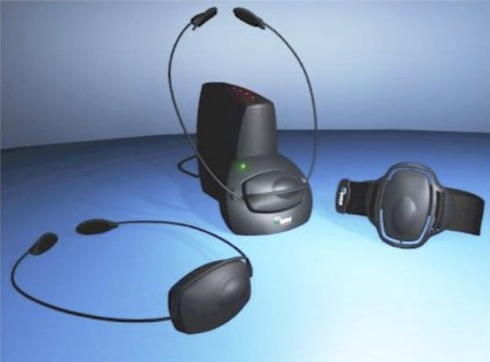
\includegraphics[width=\columnwidth]{figures/emginterface.jpg}
  \caption{EMG and Gyro-based Position Controller: Arm Bands, Head Bands, and Base.}
  \label{Tanaka:fig:emgcontroller}
\end{figure}

It is extremely important for the performer to understand that the EMG measures muscle activity that might or might not reflect muscle motion \cite{Tanaka:1993}.  For example, if an EMG electrode array were placed above the bicep and the performer were holding a heavy object steady in the bent arm position, there would be a great deal of EMG activity, with no corresponding movement.   Conversely, the arm could be relaxed causing a subsequently large movement of the arm which would not be recorded by the EMG. Thus, EMG measures isometric (no motion) activity extremely well, but isotonic (motion, but no change in tension) activity relatively poorly. 
 
Localized motion sensors such as accelerometers, gyroscopes, or levelers are far superior in measuring isotonic activity than the EMG. Thus, the addition of motion sensing to EMG sensing could create multimodal interaction to make a more expressive and complete interface.

As will be discussed in detail below, these two modes of interaction, position and EMG, can be thought of as demonstrating Oviatt's bi-directional complementarity.  That is, ``position'' could be thought of as the primary control with tension augmenting or modifying the positional information.  Vice versa, tension could be the primary control with position augmenting or modifying.  While this combination would be powerful in itself, the fact that both the tension and positional information can be multichannel creates a highly fluid, multidimensional, multimodal interaction environment.
  
In the proposed system, EMG electrodes are used in conjunction with gyroscopic sensors. The EMG surface recording electrodes are both conventional electrolyte-based electrodes and  more avant-garde active dry electrodes that use metal bars to make electrical contact with the skin. The EMG signal is acquired as a differential electrical signal. Instrumentation amplifiers on the electrodes themselves amplify and filter the signal before transmitting to the main interface unit.

The gyroscope sensors utilize a miniature electromechanical system. The device measures rotation and inertial displacement along two orthogonal axes.
The EMG and gyroscope information are then digitized. The amplitude envelope of the EMG is extracted via a straightforward RMS calculation. The Gyroscope data is accumulated over time to derive relative position information.


\section{Applying Multimodel Interaction Principles To Musical Control}


\subsection{Music as Use Case for Multimodal HCI}


Music performance is an activity that is well suited as a target for multimodal HCI concepts. Musical instruments for computer music performance are typically free-standing interface systems separate from the host computer system. They are thus well suited to explore the area in between the \textit{human-centered} and \textit{system-centered} views mentioned above. As music is by nature a time-based form, it is a medium particularly suited for investigations of temporal constraints. 

Music is a nonverbal form of articulation that requires both logical precision and intuitive expression. Sensor-based interactive devices have found application as instruments that facilitate real time gestural articulation of computer music. Most research in this domain \cite{:2000c} has focused on the musical mapping of gestural input. Given this focus on coherent mapping strategies, research has generally tended to isolate specific sensor technologies, relating them to a particular mapping algorithm to study their musical potential. 

Some sensor based musical instrument systems have been conceived \cite{Waisvisz:1985} that unite heterogeneous sensing techniques. We can think of these systems as prototypical multimodal interfaces for computer music. Such instruments might unite discrete sensors (such as switches) on the same device that also contains a continuous sensor (such as position). Operation of the continuous sensor could have different musical effect depending on the state of the discrete sensor, creating multiple modes for the use of a given sensor.


\subsection{Complementarity}


Seen in this light, traditional musical instruments can be thought of as multimodal HCI devices. Following the example given above, a piano has keys that discretize the continuous space of sound frequency. Pedals operated by the feet augment the function of the keys played by the fingers. Playing the same key always sounds the same note, but that articulates normally, muted, or sustained, depending on the state of the left and right pedals. This is a case of simple complementarity, where a main gesture is augmented by a secondary gesture.

With a stringed instrument such as the violin, multiple modes of interaction are exploited on single limb types. Bowing with one arm sets a string into vibration. Fingering with the hand on the other arm sets the base frequency of that same string. Meanwhile, multiple modes of interaction on the fingering hand enrich the pitch articulation on the string. Placing the finger on the string determines the basic pitch. Meanwhile, vibrato action with that same finger represents action with the same member in an orthogonal axis to modulate the frequency of the resulting sound. 

A case of co-dependent complementarity is seen in a woodwind instrument such as the clarinet. Two modes of interaction with the instrument work in essential combination to allow the performer to produce sound---a blowing action creates the air pressure waves while a fingering action determines the frequency. This is also a case where the two modes of interaction become more distinct one from the other: one is an interface for the mouth while the other is an interface for the hands. These two modes of interaction fuse to heighten our capability on the instrument. The complementarity is of a more equal nature than the pedal of a piano augmenting the articulation of the fingers. However, the complementarity remains unidirectional: the breath is still the main gesture essential for producing sound while the fingers augment the frequency dimension of articulation. Breathing without fingering will still produce a sound whereas fingering without breathing will not produce the normal tone associated with the clarinet.

With these examples, we observe that notions of multimodal interaction are present in traditional musical instrument technique. However, the nature of the complementarity tends to be unidirectional.

 
\subsection{Bidirectional Complementarity}

 
 There are two directions in which the notion of complementarity can be expanded. In the cases described above, discrete interventions typically augment a continuous action (albeit in the case of violin vibrato it is the converse).  One case in traditional musical performance practice that approaches use of two continuous modes is with conducting. The conductor articulates through arm gestures, but targets via gaze in a continuous visual space \cite{Usa:1998}.  However, the complementarity is still unidirectional---by gazing alone, the conductor is not accomplishing his task. The gaze direction supplements the essential conducting action.

The two sources of interaction in the system we propose, position sensing and EMG, are independent but not orthogonal, creating the possibility of \textit{bidirectional complementarity}. Each mode of interaction is sufficiently robust to be a freestanding mode of gesture--sound articulation. Musical instruments have been built using EMG alone and position sensing alone. Yet put in a complementary situation, each mode can benefit and expand on its basic range of articulation. EMG can complement position: Position/movement sensing can create the basic musical output while EMG can modulate this musical output to render it more expressive. Position can complement EMG: EMG can create the basic musical output while position sensing can create a Cartesian ``articulation space'' in which similar EMG trajectories can take on different meaning according to position.

  \begin{figure}[!htbp]
  \centering
  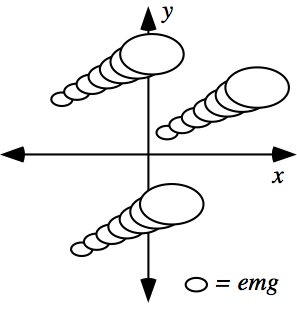
\includegraphics[scale=1]{figures/bidirectionalA.png}
  \caption{Bidirectional complementarity A: Position data complementing EMG gesture.}
  \label{Tanaka:fig:bidirectionalA}
\end{figure}

  \begin{figure}[!htbp]
  \centering
  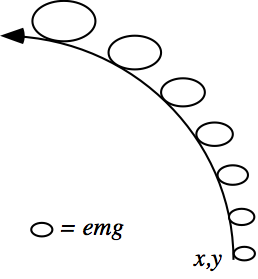
\includegraphics[scale=1]{figures/bidirectionalB.png}
  \caption{Bidirectional complementarity B: EMG data complementing positional displacement gesture.}
  \label{Tanaka:fig:bidirectionalB}
\end{figure}
 
\section{Requirements For Multimodal Musical Interaction}


\subsection{Efficiency of articulation and communication}


The net effect of expanding a sensor-based musical instrument system to be a multimodal interface must be a beneficial one. Judging the benefits of such enhanced interactivity in music differs from evaluating efficacy of task-oriented procedures. As music blends a subjective element to technical execution, evaluation of the system must also be considered on these multiple levels. 

\subsection{Multitasking vs. Multimodal}


Divergent multitasking should not be confused with focused multimodal interaction. For example, driving a car and talking on a mobile phone simultaneously is a case of the former. In such a situation, each activity is in fact hampered by the other---rather than heightening productivity, the subject finishes by executing both tasks poorly. Focused multimodal interaction should operate in a beneficial sense. If there are shortcomings in one mode, they should be compensated by enhancement \textit{afforded} by the other. As mentioned previously, this notion of \textit{mutual compensation} is a fundamental concept in multimodal HCI theory \cite{Oviatt:2003}. To what extent does it apply to musical practice?

Music as a performative form maintains criteria distinct from the pure efficiency standards of productivity studies. States of heightened musical productivity can be considered musically unsatisfying. In the case of a mechanical one-man-band, a fantastic mechanical apparatus is constructed to allow one person to play all the instruments of a band---from the various drums and cymbals to trumpet to organ. Caricatures of such a contraption evoke images of a musically silly situation. Why should a system optimized to allow a single user to interact with multiple musical instruments be considered a musical joke? Because there is the implicit understanding that the resulting music will be less effective than a real band of separate instruments. 

This example follows to some degree the example of driving and telephoning. By trying to do many things, one finishes but doing them all poorly. However, while driving and telephoning are distinct tasks, precluding its consideration as multimodal interaction, the one-man band can be considered a single musical device with multiple points of interaction. While the goal at hand is the single task of making music, this particular case of multiple modes is a musically unsuccessful one. 


\subsection{Defining a Successful Multimodal Interface}


A set of goals, then, needs to be put forth to help evaluate the effectiveness of musical interaction. The example above points out that maximizing the amount of pure productivity is not necessarily a musically positive result. Success of interactivity in music needs to be considered from the perspectives of both the performer and the listener. The goal is to attain musical satisfaction for each party. For the performer, this means a sense of articulative freedom and expressivity. The interfaces should provide modes of interaction that are intuitive to allow the performer to articulate his musical intention (control) at the same time allow him to ``let go.'' For the listener, computer based sounds are typically a family of sounds with little grounding in associative memory. Making sense of the gesture-sound interaction is a first requirement for achieving musical satisfaction \cite{Tanaka:2000}. However, at some moment, the audience also must be free to let go and have the possibility to forget the technical underpinnings of the action at hand and to appreciate the musical situation at a holistic level. A successful interactive music system should satisfy this level of intuition both for the performer and for the listener.

\subsection{Intuition}


This description of musical requirements outlined above point out likely criteria that need to be fulfilled at the interface level. Clarity of interaction is a fundamental requirement that is the basis of communication \cite{Tanaka:2000}---for feedback from the instrument back to the performer, and for transmission to the listener. However clarity alone is not enough---in fact an overly simplistic system will quickly be rendered banal. Interaction clarity can then perhaps be considered as an interim goal towards a more holistic musical satisfaction. The interfaces and modes of interactions then must be capable of creating a transparent situation where in the ideal situation the interface itself can be forgotten. By functioning at the level of intuition that allows performer and listener perception to overcome the mechanics of interaction, a musical communicative channel is established that is catalyzed by the modes of interaction, but not hindered by them.

\subsection{Expansion vs. Fusion}


While multimodal HCI discussion often focuses on \textit{fusion}, musical performance can exhibit different needs. A musical goal may not be so straightforward as the contribution of several interactions to a single result. Instead, articulative richness is a musical a goal that can be defined as different modes of interaction are contributing to distinct musical subtasks \cite{Tanaka:2001a}. The multiple modes of interaction allow simultaneous access to these articulation layers, enhancing the expressive potential of the performer. Seen in this light, multiple modes of interaction do not necessarily need to fuse towards one task, but can expand the potential of a musical gesture.  Thus complementarity is more important than fusion. 

\section{Application To Live Performance}


To demonstrate the capability of the multimodal, multichannel system proposed in this paper to enhance musical composition and performance, the authors have undertaken the development of a concert piece using EMG and relative position sensing. The piece, entitled \textit{Tibet}, includes an acoustical component in addition to the multimodal gesture sensing.  The acoustical component is created by circular bowing of resonant bowls. These bowls will be separated in space as well as pitch. These acoustic sounds, created by physical interaction, are extended by sampling and processing. This extended sonic vocabulary is articulated using a combination of gestures extracted from muscle and position sensors placed on the performer's arms. The results are complex textures in space, frequency, and time.  

  \begin{figure}[!htbp]
  \centering
  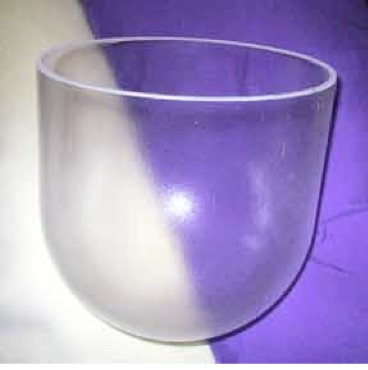
\includegraphics[scale=0.5]{figures/bowl.jpg}
  \caption{Acoustical crystal bowl .}
  \label{Tanaka:fig:crystalbowl}
\end{figure}

The piece explores the interstitial spaces between acoustic sound and electronic sound, between movement and tension, between contact and telepathy. Multiple, complimentary modes of interaction are called upon to explore these spaces. Physical contact elicits acoustical sound. These gestures are tracked as EMG data, allowing an electronic sonic sculpting that augments the original acoustic sound. In a second mode, the biosignal can continue to articulate sounds in the absence of physical contact with the bowls. In a third mode, the EMG based articulation of the sound is itself then augmented by position sensors. The position sensors give topological sense to the otherwise tension-based EMG data. Similar muscle gestures then take on different meaning in different points in space. Here we explore the articulatory space of complementary sensor systems. The piece finishes with the return of physical contact, keeping the EMG and position sensing in a unified gestural expression.


\section{Conclusions}


The approach introduced in this paper combines criteria established in the two fields of multimodal HCI research and gestural music interface research. With this we have defined design goals for what constitutes a musically successful implementation of multimodal interaction. We believe that the system proposed in this paper, using EMG in conjunction with relative position sensing, achieves the outlined goals of a successful multimodal musical interface:

\begin{enumerate}
\item Each of the component modes are intuitive interfaces 
\item The multimode context leverages the richness of each interface to expand the articulative range of the other
\item The two interfaces are independent and yet exhibit bi-directional complementarity

\end{enumerate}

We have reviewed the fundamentals of multimodal human computer interaction as applied to musical performance. In this paper, we have described specificities of music that make it apt for the application of multimodal HCI concepts. We have indicated other characteristics of music that allow us to expand on the single task orientation of classical multimodal HCI research. We proposed a multimodal gestural music system based on biosignals and relative position sensing. We introduce the notion of \textit{bidirectional complementarity} that defines the interdependent relationship between the two sensing systems and establishes the richness of interaction required and afforded by music.  Finally, we have described a musical piece that demonstrates the interaction capabilities of the proposed system.
 

\begin{acknowledgement}
\
The authors would like to thank Sony CSL and Moto Development Group for supporting this work.
\end{acknowledgement}

\section*{Author commentary: Multimodal musical interaction, a decade later}
\paragraph{Atau Tanaka and R. Benjamin Knapp}

The technologies we enthusiastically wrote about in 2002 are now readily available, and are quickly becoming mainstream. There are consumer EMG devices that have been Kickstarted\footnote{\url{http://www.myo.com}} as well as devices that expand the use of electrophysiology from the somatic (EMG) to the autonomic nervous system (signals such as the EDA and HR).\footnote{\url{http://www.empatica.com}} These consumer-grade devices can give clean enough data to be useful in research, opening up the range of potential creative applications in NIME. Many of these devices integrate physical sensing alongside physiological sensing, making them multimodal. The ideas we wrote about over a decade ago, on the use of multiple modes of interaction for music, have arrived in commercially available technologies, and are available to all musicians and artists. This increased accessibility has not lessened the research challenges, however, and the core scientific imperatives remain. How can we best make use of multiple modes of interaction with gestural input to create rich musical results? As we deepen our study of multimodal interaction and connect that to human capabilities of intermodal perception, we sharpen our research focus. 

%Meanwhile, the more we know, the more there is to verify, risking to turn the research incremental.

The distinction we made in the original paper between ``human-centered'' and ``system-centered'' views are not as clear cut today as they used to be. In fact they are fundamentally intertwined in the design of modern interactive systems. Research in infant cognitive development shows that intermodal perception is innate, as well as learned. 
% \cite{thelen1996dynamic}. 
This means that we naturally use multiple sensory modes to make sense of events in the world. At the same time, we learn new links, and are capable of forming cross-modal mappings that are not inherent. Increasingly, interaction design is informed by this knowledge of cognitive processes. Today, we build interactive systems that support these human capabilities, making the system-view inherently human-centric.

The focus on ``control'' in the original paper belies the era in which it was written. The turn of the  new millennium, coming out of two decades of MIDI, was a technologically more deterministic time. Today we are less positivist, preferring to look at human-machine relationships where control may not be desired nor possible. Indeed, the evolution of this work to include affect measurement has challenged what the word, control, means in the context of the modern digital musical instrument. Input/output mappings go beyond the classical one-to-many and many-to-one paradigms to also include direct sonification, audification, input modeling, and feature mapping.

Despite these advancements in thinking, the core literature on multimodal interaction reviewed in the paper continues to be essential reading. They remind us of important concepts such as fusion, temporal constraints, and complementarity. In our present-day, lightspeed scans of Google Scholar and the ACM Digital Library, it's easy to overlook this foundational literature. Re-reading our own paper even as we continue these lines of research was an eye opener for us.  There have since been important advancements in novel methods, such as the use of sensory substitution in the interface \cite{Bach-y-Rita:2003}, and the codification of multimodal interaction in methodological frameworks \cite{Norris:2004}.

The sections relating multimodal concepts to  musical practice are, in retrospect and in the spirit of self-criticism, quaintly naive. The comparisons we made at the time to piano and violin performance practice and conducting are in fact examples of multi-channel input and not multimodal interaction \textit{per se}. Indeed, the section distinguishing musical practice from task based performance, though true, is speculative, and shows the romantic possibility of research back then. Today, the availability of ready tools, and the advancement of research in these topics fence us into forms of rigor, that, if not intellectually constraining, make us more incremental in the claims we put forth.

The core work reported in the original paper is, we believe, still useful today. Physiological sensing via the EMG can complement inertial position sensing, and vice versa. Bi-directional complementarity is a good way to frame the mutually reinforcing nature of these multimodal relationships.

We have since continued this research. The EMG has been put in bi-modal contexts alongside biophysical sensing of the mechano-myogram (MMG) and we have studied the EMG in multimodal contexts with motion capture systems in addition to accelerometers. We have looked more closely at the EMG signal itself, in conjunction with the MMG \cite{Donnarumma:2013}, and to see how feature extraction can pre-process the bio-signal for subsequent machine learning analysis \cite{Caramiaux:2015}.  We have explored how EMG can be one component of an affective interface \cite{Knapp:2011}. We have studied how musicians and non-musicians can produce and reproduce gesture, reliably articulate expressive variation of gesture, and look at hardware and software's ability (and limits) in tracking this. Based on this, we build musical systems that are tuned to users' abilities, be they virtuostic, disabled, or lay performers.


\section*{Expert commentary: Human bodies, algorithms and intuition}
\paragraph{Marco Donnarumma}

In 2002, when this paper by Atau Tanaka and Ben Knapp was published, the NIME conference was just at its second edition. While the NIME community had been formalised only the year before, the uniquely inventive and cross-disciplinary spirit grounding the design and performance with new musical instruments had been nurtured since much longer \cite{Krefeld:1990,Moore:1988}. The individual and joint research by Tanaka and Knapp in particular has been seminal to different areas of NIME research: from gestural interaction to hardware design, from biomusic to mobile music. Tanaka and Knapp's approach to new musical instrument performance has been, and still is, as much idiosyncratic as innovative. They had been collaborating since the late 1980s, when Knapp and Hugh Lusted commissioned Tanaka the creation of the first musical piece for their bioelectrical musical interface, the Biomuse. In \textit{Kagami}, the related piece created by Tanaka and premiered in 1992 at CCRMA Stanford, Tanaka, Knapp and Lusted used armbands embedded with wet electrodes to capture electrical discharges from the performer's forearm and upper arm muscles, measured as electromyogram or EMG. The electrical signals were then digitized and translated into MIDI parameters modulating a Yamaha TG77 and a Korg Wavestation.

The design and performative approach of Tanaka, Lusted and Knapp expanded the breadth of gestural performance with NIME by enabling a kind of interaction between performer and instrument that Tanaka has termed \lq visceral\rq \cite{Tanaka:2011}. For Tanaka, visceral refers to the fact that the instrument's physiological sensing affords the capture of information on the performer's intention of movement, rather than how movement is performed in space. Tanaka and Knapp's approach evolved through the years and by 2002 they presented the paper in question, which proposes a framework for multimodal interaction in music performance using two sensing modalities, EMG and relative position sensing. Combining multimodal interaction methods, developed in the field of human-computer interaction (HCI), and gestural control of computer-based musical instrument,  the article discusses the use of those two independent, and yet complementary, sensing modalities to increase the level of expressive musical articulation available to the performer. The paper also offers insights on a practical application of the multimodal framework to \textit{Tibet}, a piece that was performed at the same conference. The article provided two major contributions to the NIME community. First, it formally introduced the basic properties of EMG sensing in the context of real-time musical interaction with computer-based instruments, a sensing modality that had been described on other occasions by the same authors, but not yet in the specific context of NIME. Second, it elaborated on a set of multimodal sensing methods in HCI and thus identified the most suitable for musical performance, that of bidirectional complementarity, where independent sensing modalities can take advantage from, and extend, each other. A light weakness of the paper lies in that the two ending sections bring the discussion to a hasty close, and we are left with an exciting prospect and only few hints of its potential in a real-world performance. The interested reader can refer to an online video excerpt of the related performance, \textit{Tibet},\footnote{\url{https://www.youtube.com/watch?v=O_z0hdS4umY}} by Atau Tanaka.

However, what makes this paper highly significant to our present community is, to my view, the way in which the contributions are framed. The article does not focus on technical insights on the use of biosignals or gyroscope data; rather, it contends the capacity of the proposed multimodal approach to create room for intuition, bodily skill, control and lack thereof, in musical gestural interaction. This is an approach to NIME performance that balances technical insight with bodily performance, algorithms with intuition. In the past years this kind of approach has increasingly lost currency in favour of primarily technical research into the affordances of new instruments. What we can abstract thus from Tanaka and Knapp's contribution is the importance of integrating technical findings and insights on bodily performance into our research methods. This can be done by considering the importance of corporeality to performance with computer-based musical instruments. Corporeality, meaning the physical, physiological and cultural basis of embodied practices, is a foundation of musical performance, and should therefore not be seen as a minor issue in our research and practise. Rather, technical research itself can be informed by looking at how technological instruments, algorithms and sound manipulations, not only bring forth new kinds of music, but also extend, hinder or alter the properties of the performer's and the listeners' bodies \cite{Hayles:1999,Henriques:2011}. 



\graphicspath{ {mainmatter/Verplank_2002/} }
\title*{2002: The Plank: Designing a Simple Haptic Controller}
\titlerunning{A Simple Haptic Controller}

\author{Bill Verplank, Michael Gurevich and Max Mathews}
\authorrunning{Verplank et al.}

%\institute{Bill Verplank \at Center for Computer Research in Music and Acoustics, Stanford University, Stanford, California, USA \email{bill@billverplank.com} 
%\and Michael Gurevich \at University of Michigan, School of Music, Theatre \& Dance, Ann Arbor, Michigan, USA \\ \email{mdgurev@umich.edu} \\ Affiliation at time of original publication: Center for Computer Research in Music and Acoustics, Stanford University, Stanford, California, USA
%\and Max Mathews \at Center for Computer Research in Music and Acoustics, Stanford University, Stanford, California, USA}
%
% Use the package ''url.sty'' to avoid
% problems with special characters
% used in your e-mail or web address
%
\maketitle

\abstract*{Active force-feedback holds the potential for precise and rapid controls. A high performance device can be built from a surplus disk drive and controlled from an inex- pensive microcontroller. Our new design,The Plank has only one axis of force-feedback with limited range of motion. It is being used to explore methods of feeling and directly manipulating sound waves and spectra suitable for live performance of computer music.}

\section{Introduction}

In 1996, Perry Cook at Princeton, Ben Knapp at San Jose State and Chris Chafe at Stanford University started teaching a video-linked course in human-computer interaction technology. Max Mathews and Bill Verplank have in the last two years focussed the course on music controllers \cite{Verplank:2001} for the masters program in music science and technology. At CCRMA, we have a Phantom, a high-performance three-degree-of-freedom force-feedback device donated by Interval Research. We want a simpler device for experimentation and performance.

\begin{figure}[ht]
% Use the relevant command for your figure-insertion program
% to insert the figure file.
% For example, with the graphicx style use
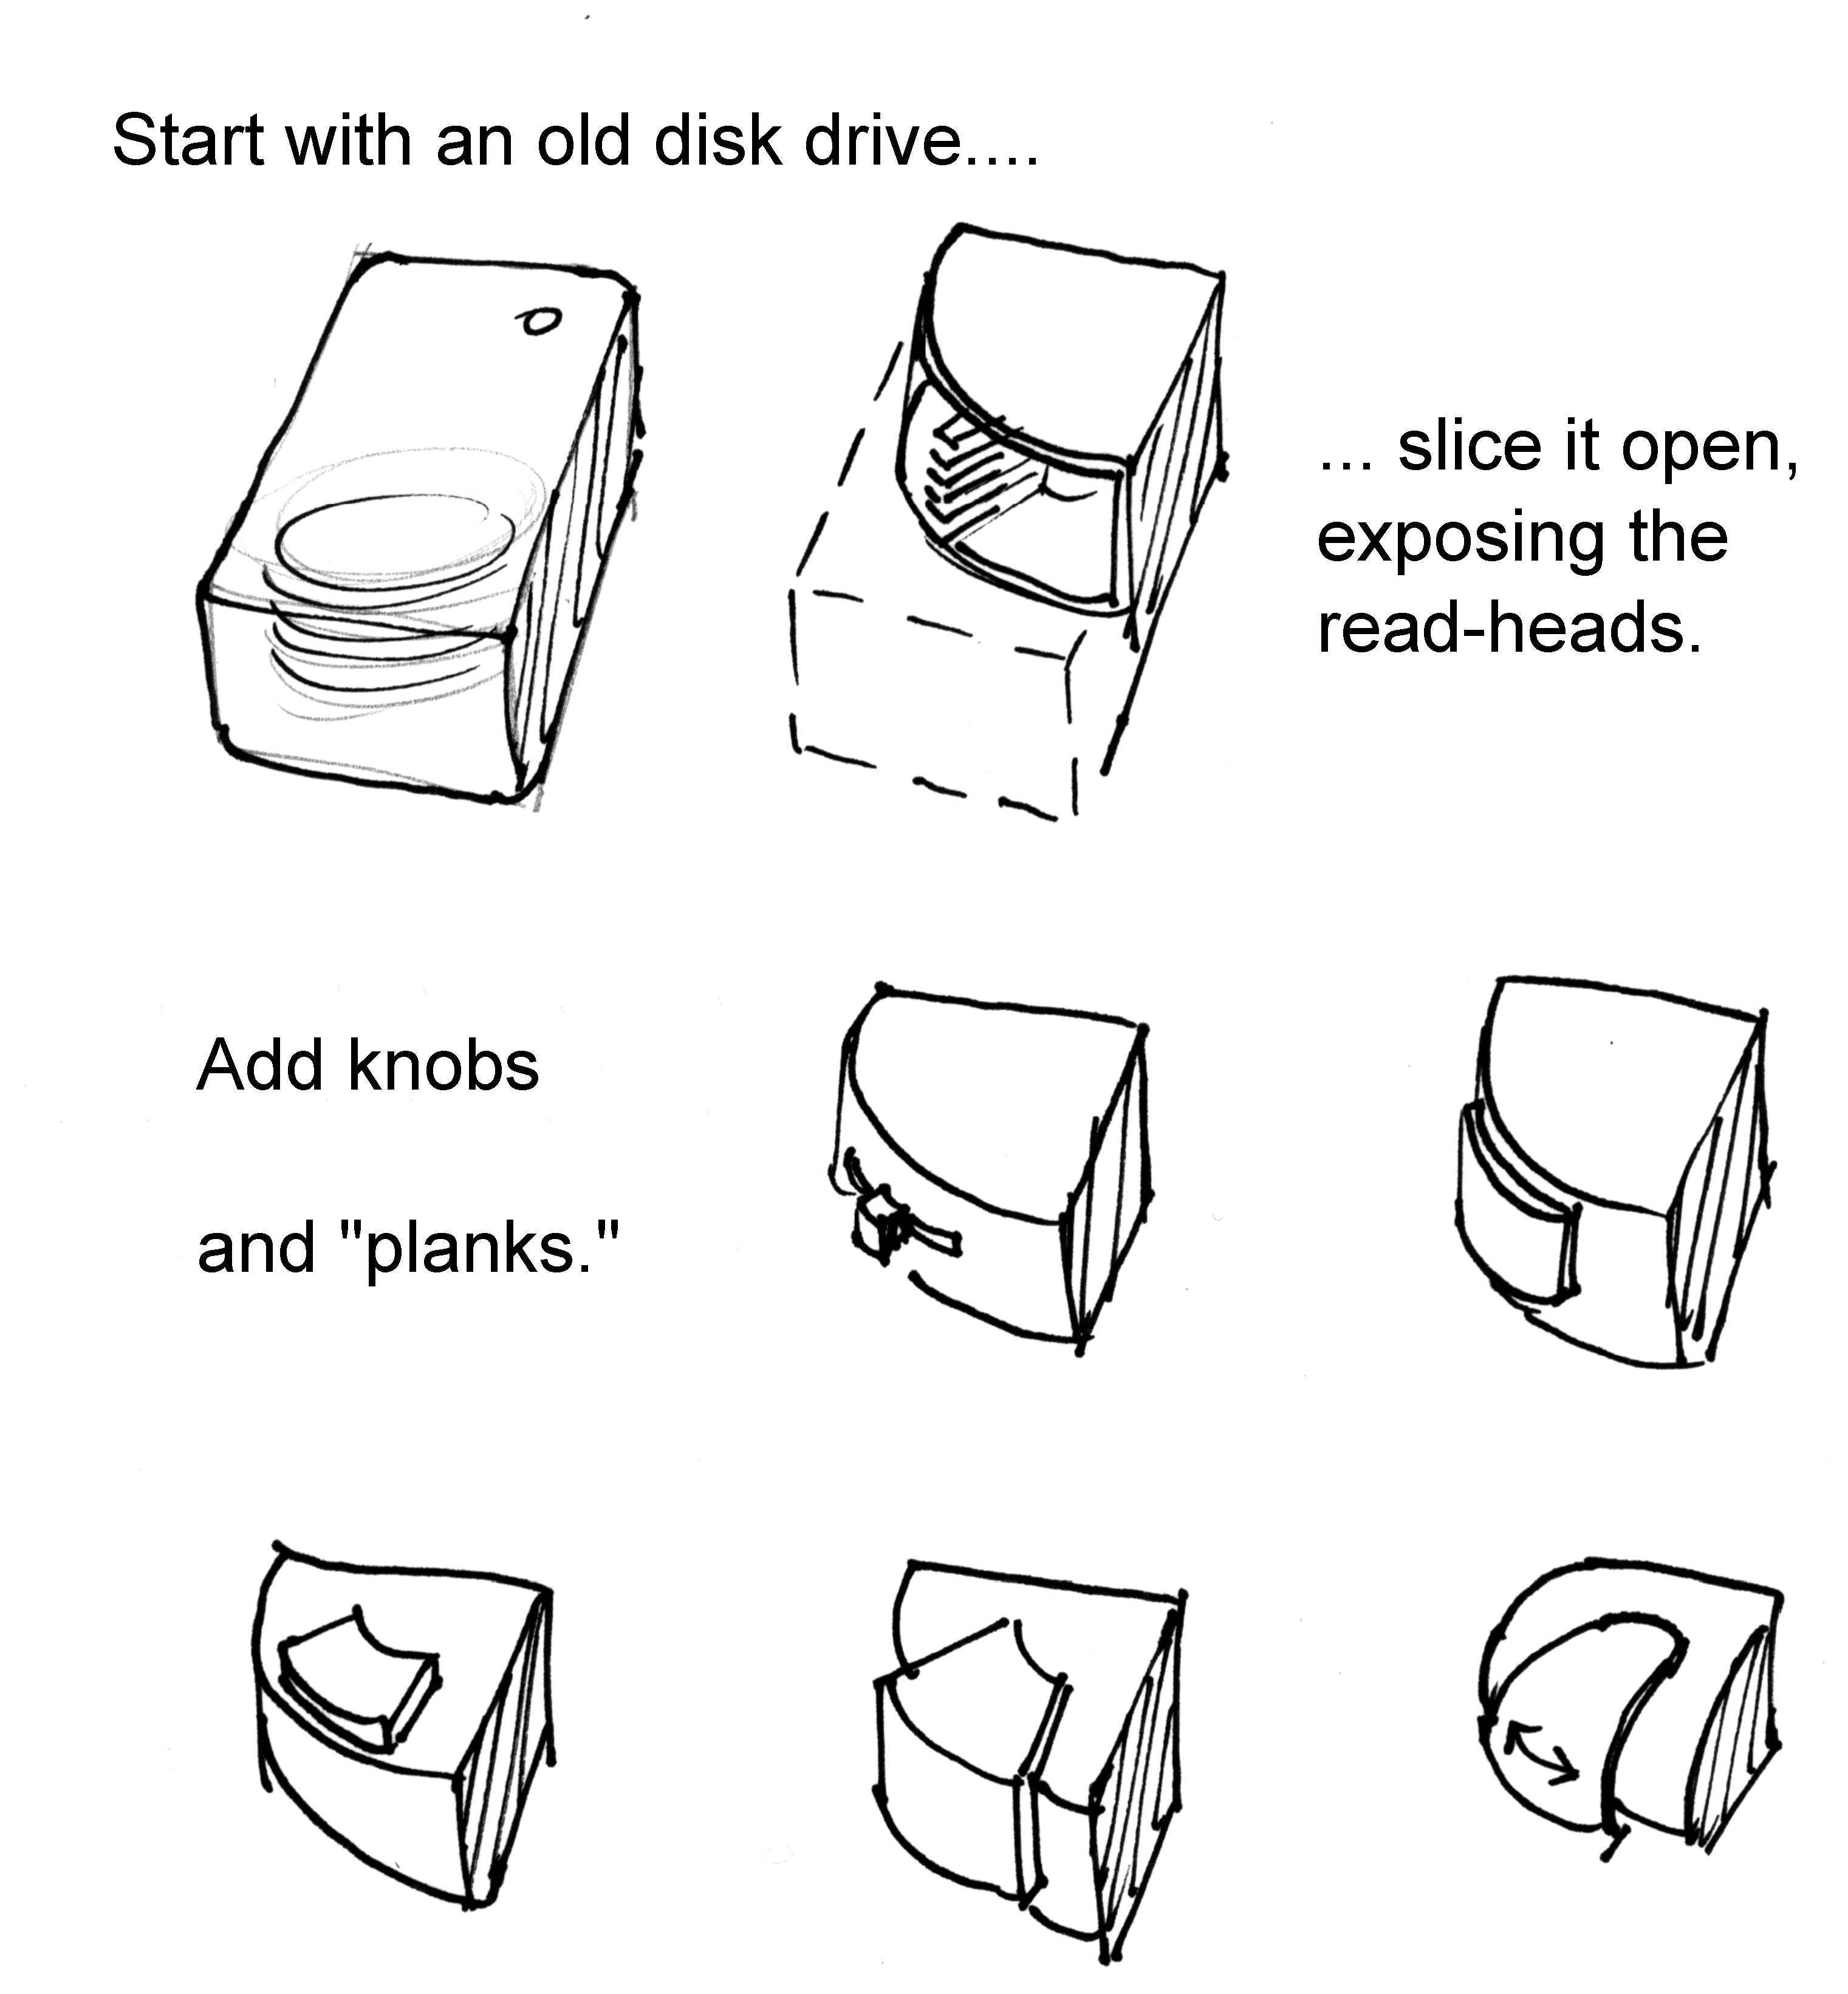
\includegraphics[width=9cm]{Plank1}
\centering

% If no graphics program available, insert a blank space i.e. use
%\picplace{5cm}{2cm} % Give the correct figure height and width in cm
%
\caption{The Plank concept}
\label{Verplank:fig:1}       % Give a unique label
\end{figure}


\subsection{Scanned Synthesis}
\label{Verplank:sub:1_1}
At Interval, we used Phantoms \cite{Massie:1994} to explore the value of force-feedback. One discovery was that simple spring-mass simulations, which are uncontrollable without force-feedback, can be controlled simply by letting the vibrating system transfer energy to the human. In feeling a simulated wave, Verplank, Shaw and Mathews had the idea of listening to the shapes. This came to be known as ``scanned synthesis'' \cite{Verplank:2000}. The idea is to directly manipulate a dynamic wave shape at human-hand frequencies while scanning the wave shape out at audio frequencies. The pitch is determined by the length of the wave and the scan rate. The timbre is determined by the wave shape which is being continuously controlled by the performer.

\subsection{Haptics}
\label{Verplank:sub:1_2}
The term haptics is used by psychologists to describe the human sense of touch including skin senses as well as muscle and joint senses. Recently, ``haptic'' devices have made it to market in vibrating pagers, rumble-packs, force-feedback joysticks, steering wheels and mice. There are active research communities and a small industry building devices. Standards have been established for communication and development. At Interval, we explored the potential for simple haptic devices for media control and expression \cite{Snibbe:2001}.

\section{Haptic Illusions}

The Plank is designed to take advantage of several illusions that allow us to reduce the device complexity while maintaining haptic fidelity. The key feature is a surface which measures forces orthogonal to its motion. With a measured surface force, the Plank simulates terrain as well as friction and dynamics.

\subsection{Slope}
\label{Verplank:sub:2_1}
When you press down on a surface, it usually pushes back on you with a ``surface normal'' perpendicular to the surface. The forces fed back by the device can give the illusion of slopes of a surface. Small variations in force as you move along the surface are felt as bumps. In a pioneering study, Margaret Minsky explored this phenomenon of simulated textures with a two-degree-of-freedom force-feedback joystick \cite{Minsky:1995}. The Plank reinforces this illusion by measuring the force applied by the user normal to the motion and making the tangential force-feedback proportional.

\begin{figure}[ht]
% Use the relevant command for your figure-insertion program
% to insert the figure file.
% For example, with the graphicx style use
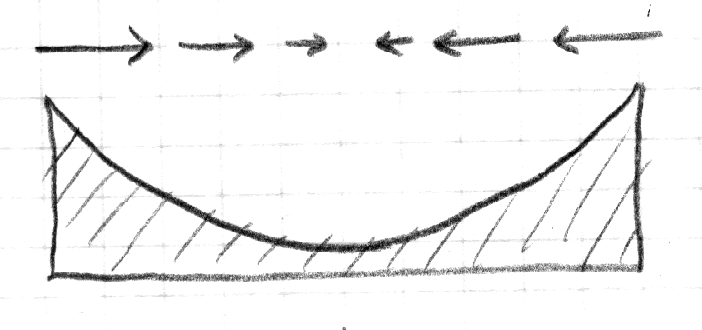
\includegraphics[width=5cm]{Plank2}
\centering

% If no graphics program available, insert a blank space i.e. use
%\picplace{5cm}{2cm} % Give the correct figure height and width in cm
%
\caption{Slope illusion}
\label{Verplank:fig:2}       % Give a unique label
\end{figure}

\subsection{Clutch}
\label{Verplank:sub:2_2}
Rob Shaw simulated a variety of dynamic systems which could be engaged by applying forces \cite{Snibbe:2001}. We came to call this phenomenon the ``haptic clutch.'' By pressing on The Plank, you engage with a simulated moving object. This technique compensates for the limited travel of The Plank and allows the illusion of wide reach.

\begin{figure}[ht]
\centering
% Use the relevant command for your figure-insertion program
% to insert the figure file.
% For example, with the graphicx style use
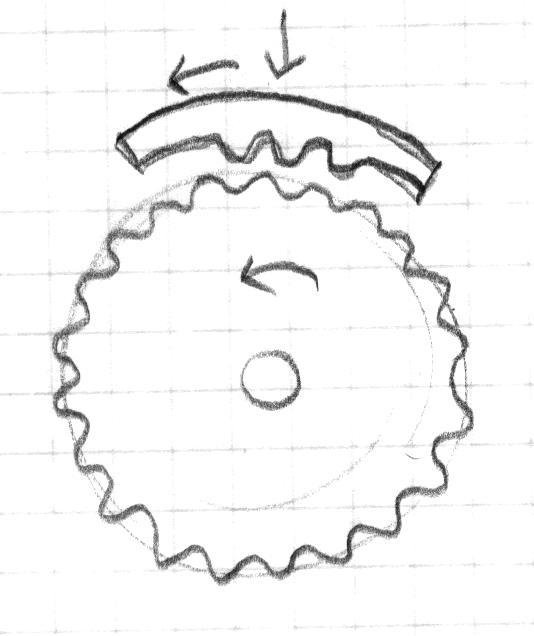
\includegraphics[width=5cm]{Plank3}
%
% If no graphics program available, insert a blank space i.e. use
%\picplace{5cm}{2cm} % Give the correct figure height and width in cm
%
\caption{The haptic clutch}
\label{Verplank:fig:3}       % Give a unique label
\end{figure}

\section{Hardware}

The construction of The Plank was undertaken as an educational exercise using inexpensive or found components. It is described in some detail with the hope that others will take on such do-it-yourself haptics.

\begin{figure}[ht]
\centering

% Use the relevant command for your figure-insertion program
% to insert the figure file.
% For example, with the graphicx style use
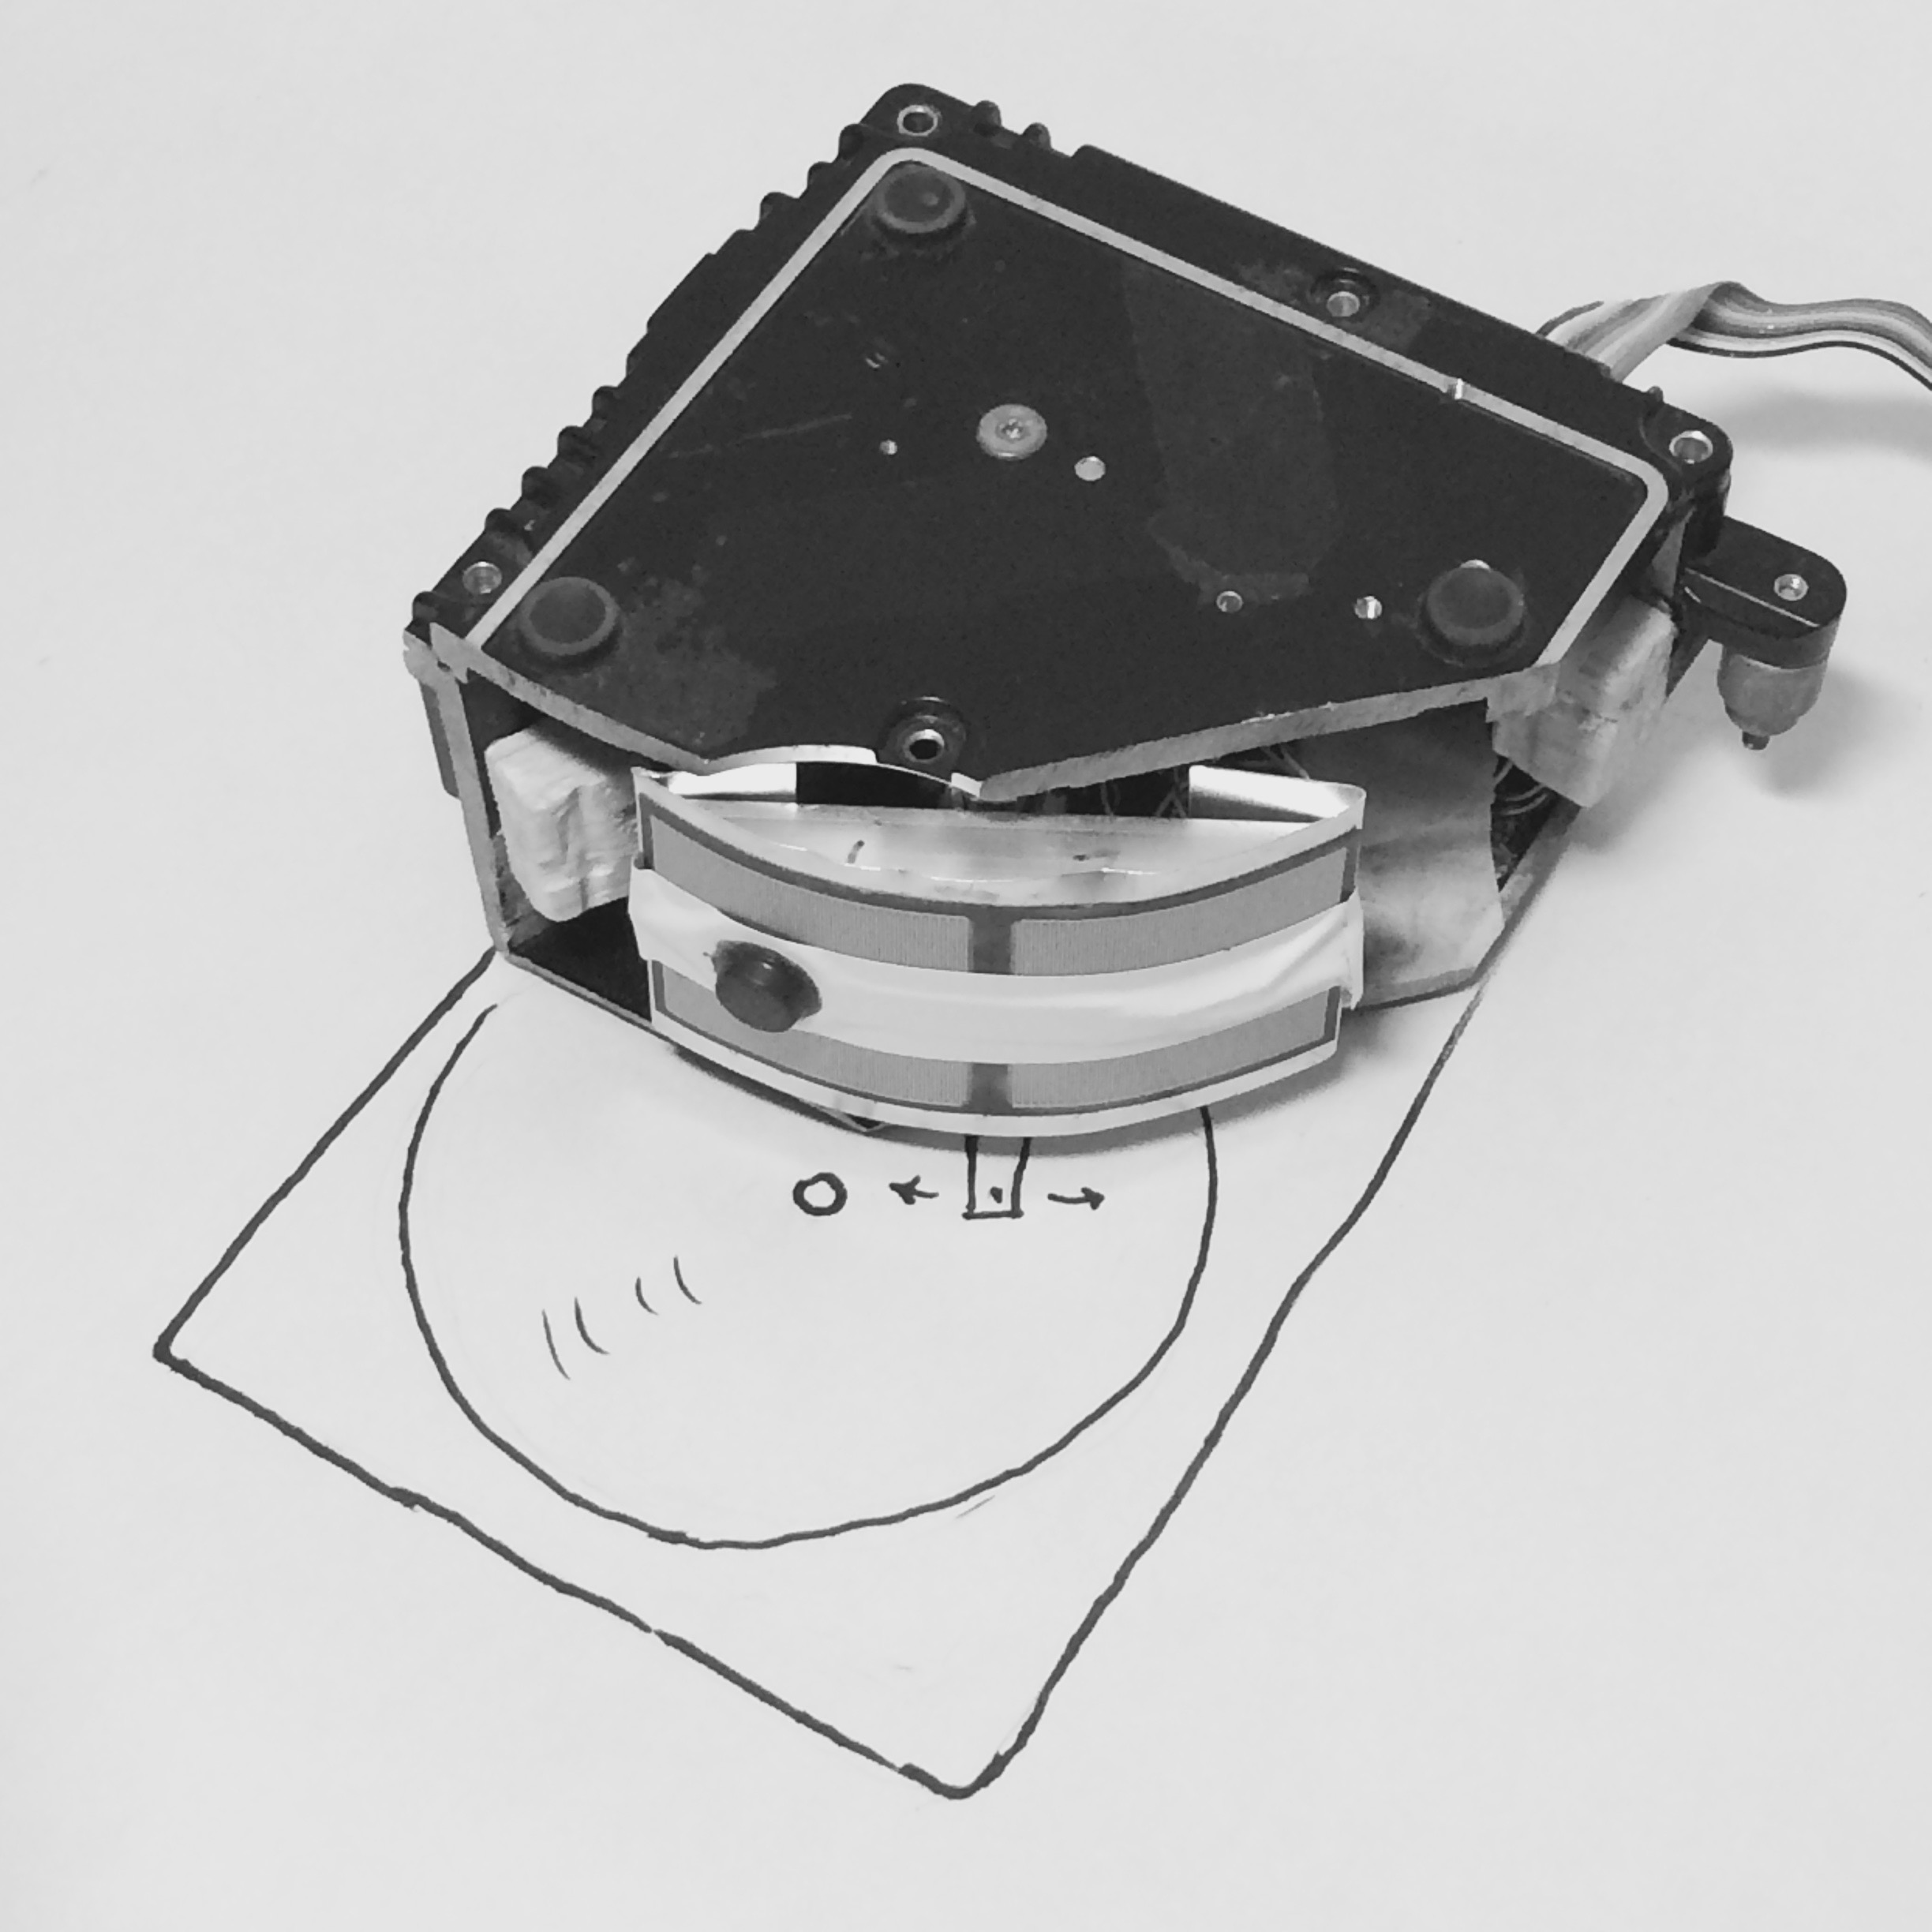
\includegraphics[width=11.3cm]{Plank4}
%
% If no graphics program available, insert a blank space i.e. use
%\picplace{5cm}{2cm} % Give the correct figure height and width in cm
%
\caption{Disk drive cutaway}
\label{Verplank:fig:4}       % Give a unique label
\end{figure}


\subsection{Motors}

Rotary DC motors are the most common actuators used for haptic display from \$1 vibrators to \$100 joysticks to \$10,000 Phantoms. In contrast, the motors chosen for The Plank are from computer disk drives where they position the read-heads. They are known as voice-coil motors. There is no requirement for gears or pulleys, both the drive and the sensor are directly coupled to the motor. Several haptic displays have been made from disk drive motors. Hong Tan studied tactile communication bandwidth with three independent disk-drive motors \cite{Tan:1996}. Pietro Buttolo built a planar mechanism for positioning the tip of a stylus using three disk-drive motors \cite{Buttolo:1995}. The voice coil motors are readily available as castoffs in crashed disks.

\subsection{Microcontroller}
\label{Verplank:sub:3_2}
To ensure rapid computation of the forces, an Atmel mega163 microcontroller is dedicated to local control of The Plank. % \cite{Atmel:}. 
It operates at up to 8 Mhz with 8 channels of 10-bit A/D ($\sim$10k samples/second), 32 I/0 ports, 16K bytes of program memory and 1024 bytes of data memory. The microcontroller has a UART for communication via MIDI with a synthesizer or real-time DSP software. Interrupts keep the sampling, or servo update at a steady rate up to 4kHz.

\subsection{Sensing and orthogonal force control}
\label{Verplank:sub:3_3}
A hall-effect sensor is used for rotary position feedback read by an 10-bit A/D converter built into the microcontroller. A 12-bit DAC commands a power op-amp for generating up to 3A current and forces up to 5 Newtons ($\sim$1 lb) at the finger tips (for short times). The sensing and power amp came from the design for a simple device used in teaching haptics \cite{Richard:1997}. Force sensitive resistors measure finger pressure on the surface of The Plank.

\begin{figure}[ht]
\centering

% Use the relevant command for your figure-insertion program
% to insert the figure file.
% For example, with the graphicx style use
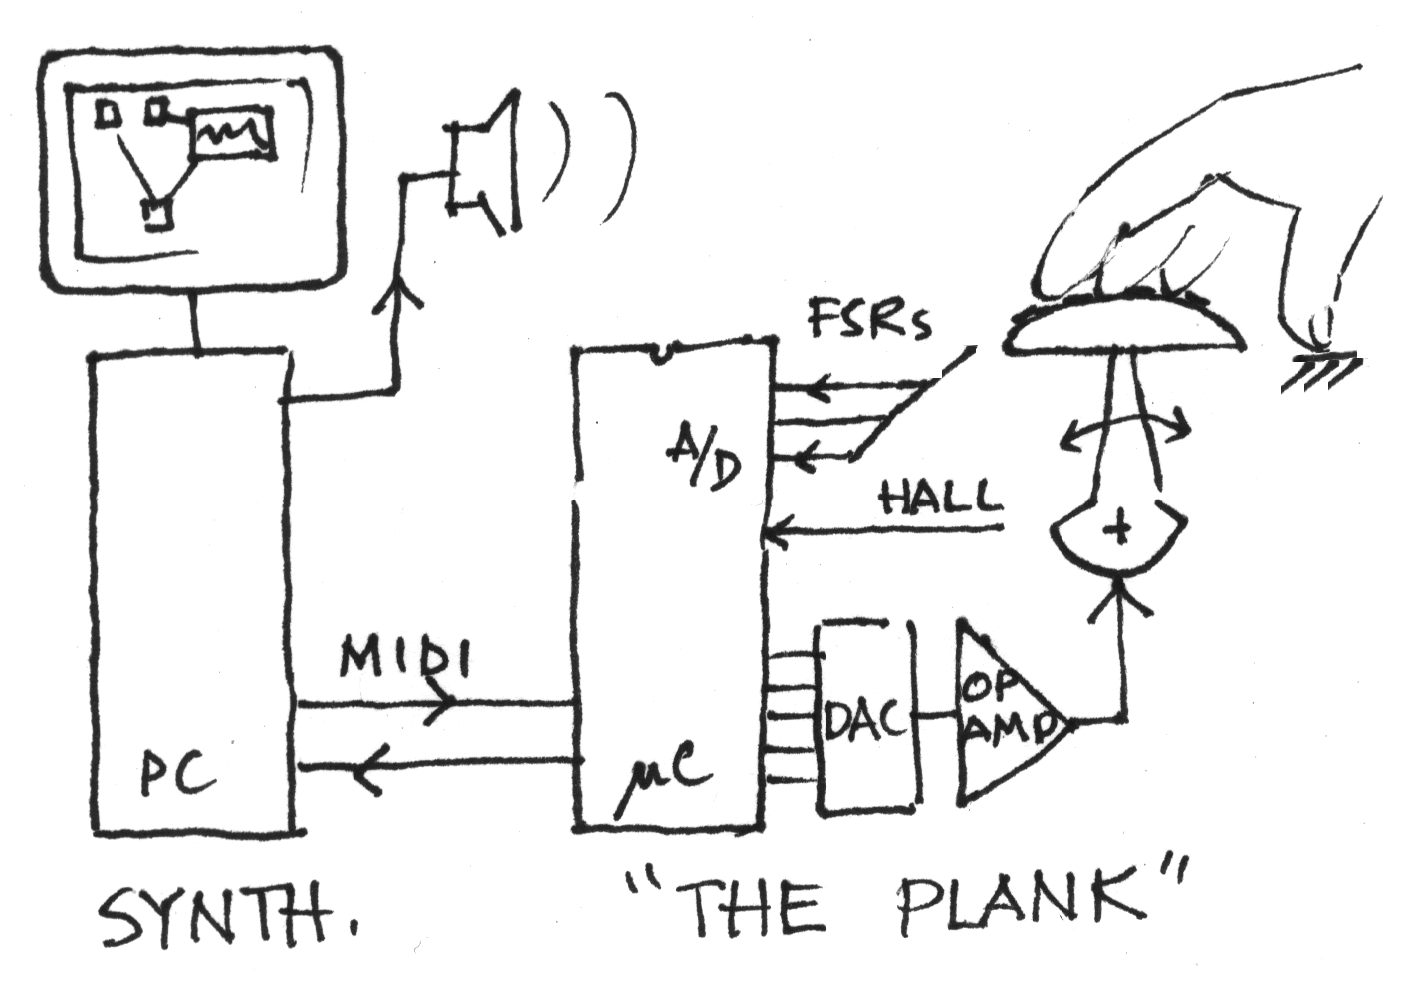
\includegraphics[width=11.3cm]{Plank5}
%
% If no graphics program available, insert a blank space i.e. use
%\picplace{5cm}{2cm} % Give the correct figure height and width in cm
%
\caption{System diagram}
\label{Verplank:fig:5}       % Give a unique label
\end{figure}

\section{Effects}

\subsection{Table of Forces: Terrain}
\label{Verplank:sub:4_1}
The microprocessor holds a small look-up table with a force for every measured position of The Plank. In scanned synthesis, the shape represents one cycle of a wave or piece of terrain. As you move The Plank, you feel the shape of the terrain; when you apply pressure, you can manipulate the terrain.


\begin{figure}[ht]
\centering

% Use the relevant command for your figure-insertion program
% to insert the figure file.
% For example, with the graphicx style use
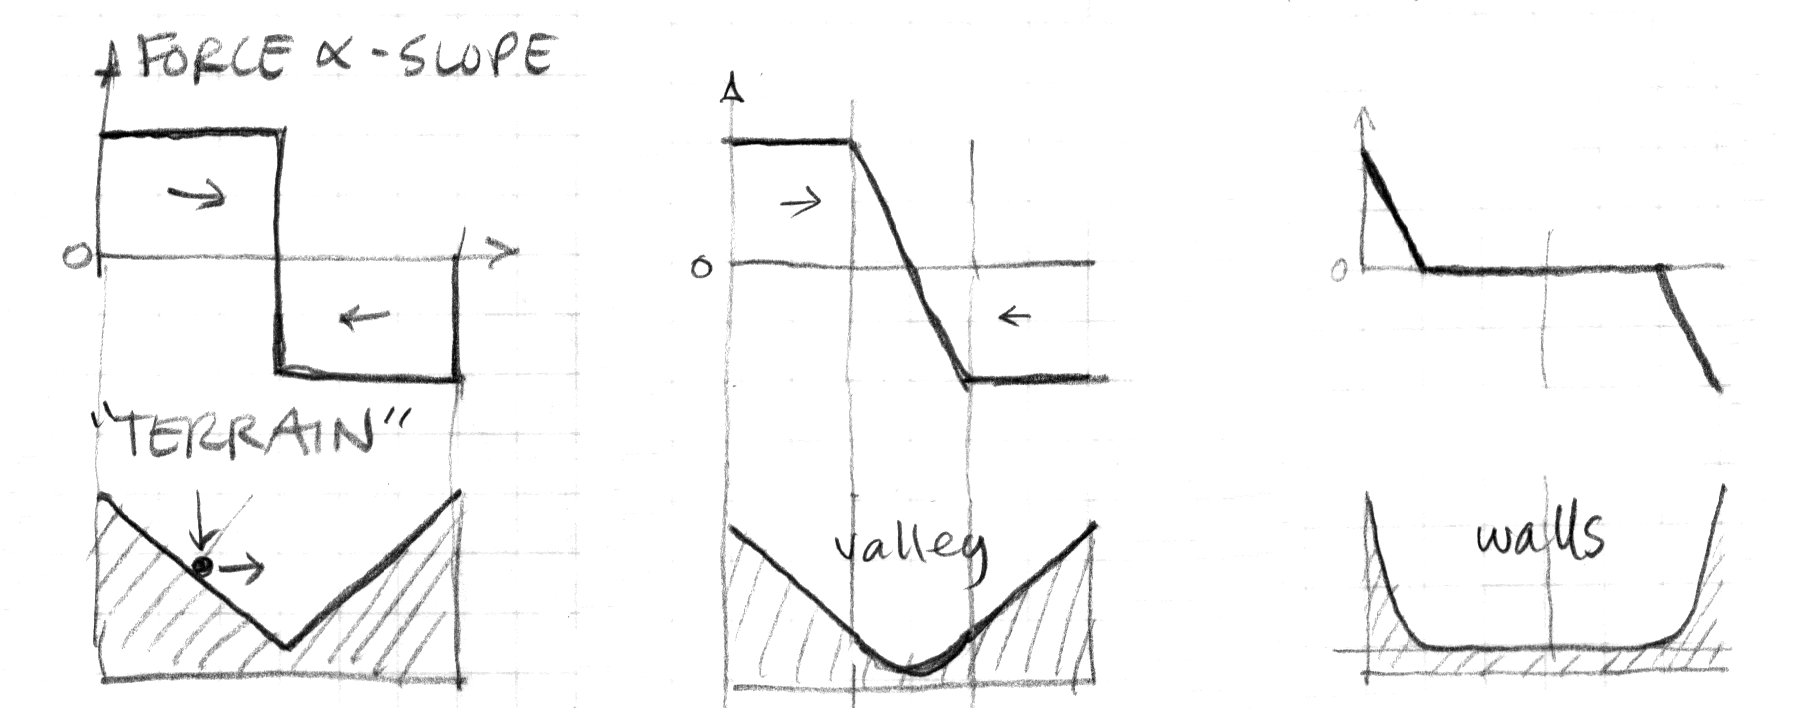
\includegraphics[width=11.3cm]{Plank6}
%
% If no graphics program available, insert a blank space i.e. use
%\picplace{5cm}{2cm} % Give the correct figure height and width in cm
%
\caption{Forces create terrain illusions}
\label{Verplank:fig:plank6}       % Give a unique label
\end{figure}

\subsection{Motion: Dynamics}

The whole terrain can be moved left or right (actually just a pointer into the table). Buffers can extend the table beyond the range of Plank motion (in the case of scanned synthesis, the table is circular and the buffers are not necessary). To simulate a single mass attached to a spring, one detent or deep valley in the terrain represents the position of the mass, its slopes represent the stiffness of the spring. The force on The Plank increases as it moves ``up the slope of the valley.'' The acceleration of the mass is simply computed from the force being fed back to The Plank.

\subsection{Friction}

We have experimented using the Phantom with several friction models. The simplest is ``stick-slip,'' Just one spring that builds up to a maximum and then ``breaks'' feels like plucking a string. When one spring breaks another can grab hold; many small ones make a fine texture that makes it easy to hold still. It is easy to add ``viscosity'' by measuring velocity and resisting the motion proportionately.
Combinations of these effects should be able to provide a wide variety of behaviors. Examples are shown in Table 1.

\begin{table}
\label{Verplank:tab:1} 
\centering
\ra{1.3}
\caption{The Plank's effects combined}
\vspace{3pt} \noindent
\begin{tabular}{llll}
\toprule
\textbf{Effect} & \textbf{Terrain} & \textbf{Dynamics} & \textbf{Friction}  \\
\midrule  
DETENTS  & Valleys  \hspace{2cm}  & --   & --\\
PLATTER & None cleavage & Inertia \hspace{2cm} & Stick-slip\\
WAVE \hspace{2cm} & Shape  & Mass/Spring & Viscosity\\
PLUCK & --  & String & Stick-slip\\
\bottomrule
\end{tabular}
\end{table}

\begin{figure}[ht]
\centering
% Use the relevant command for your figure-insertion program
% to insert the figure file.
% For example, with the graphicx style use
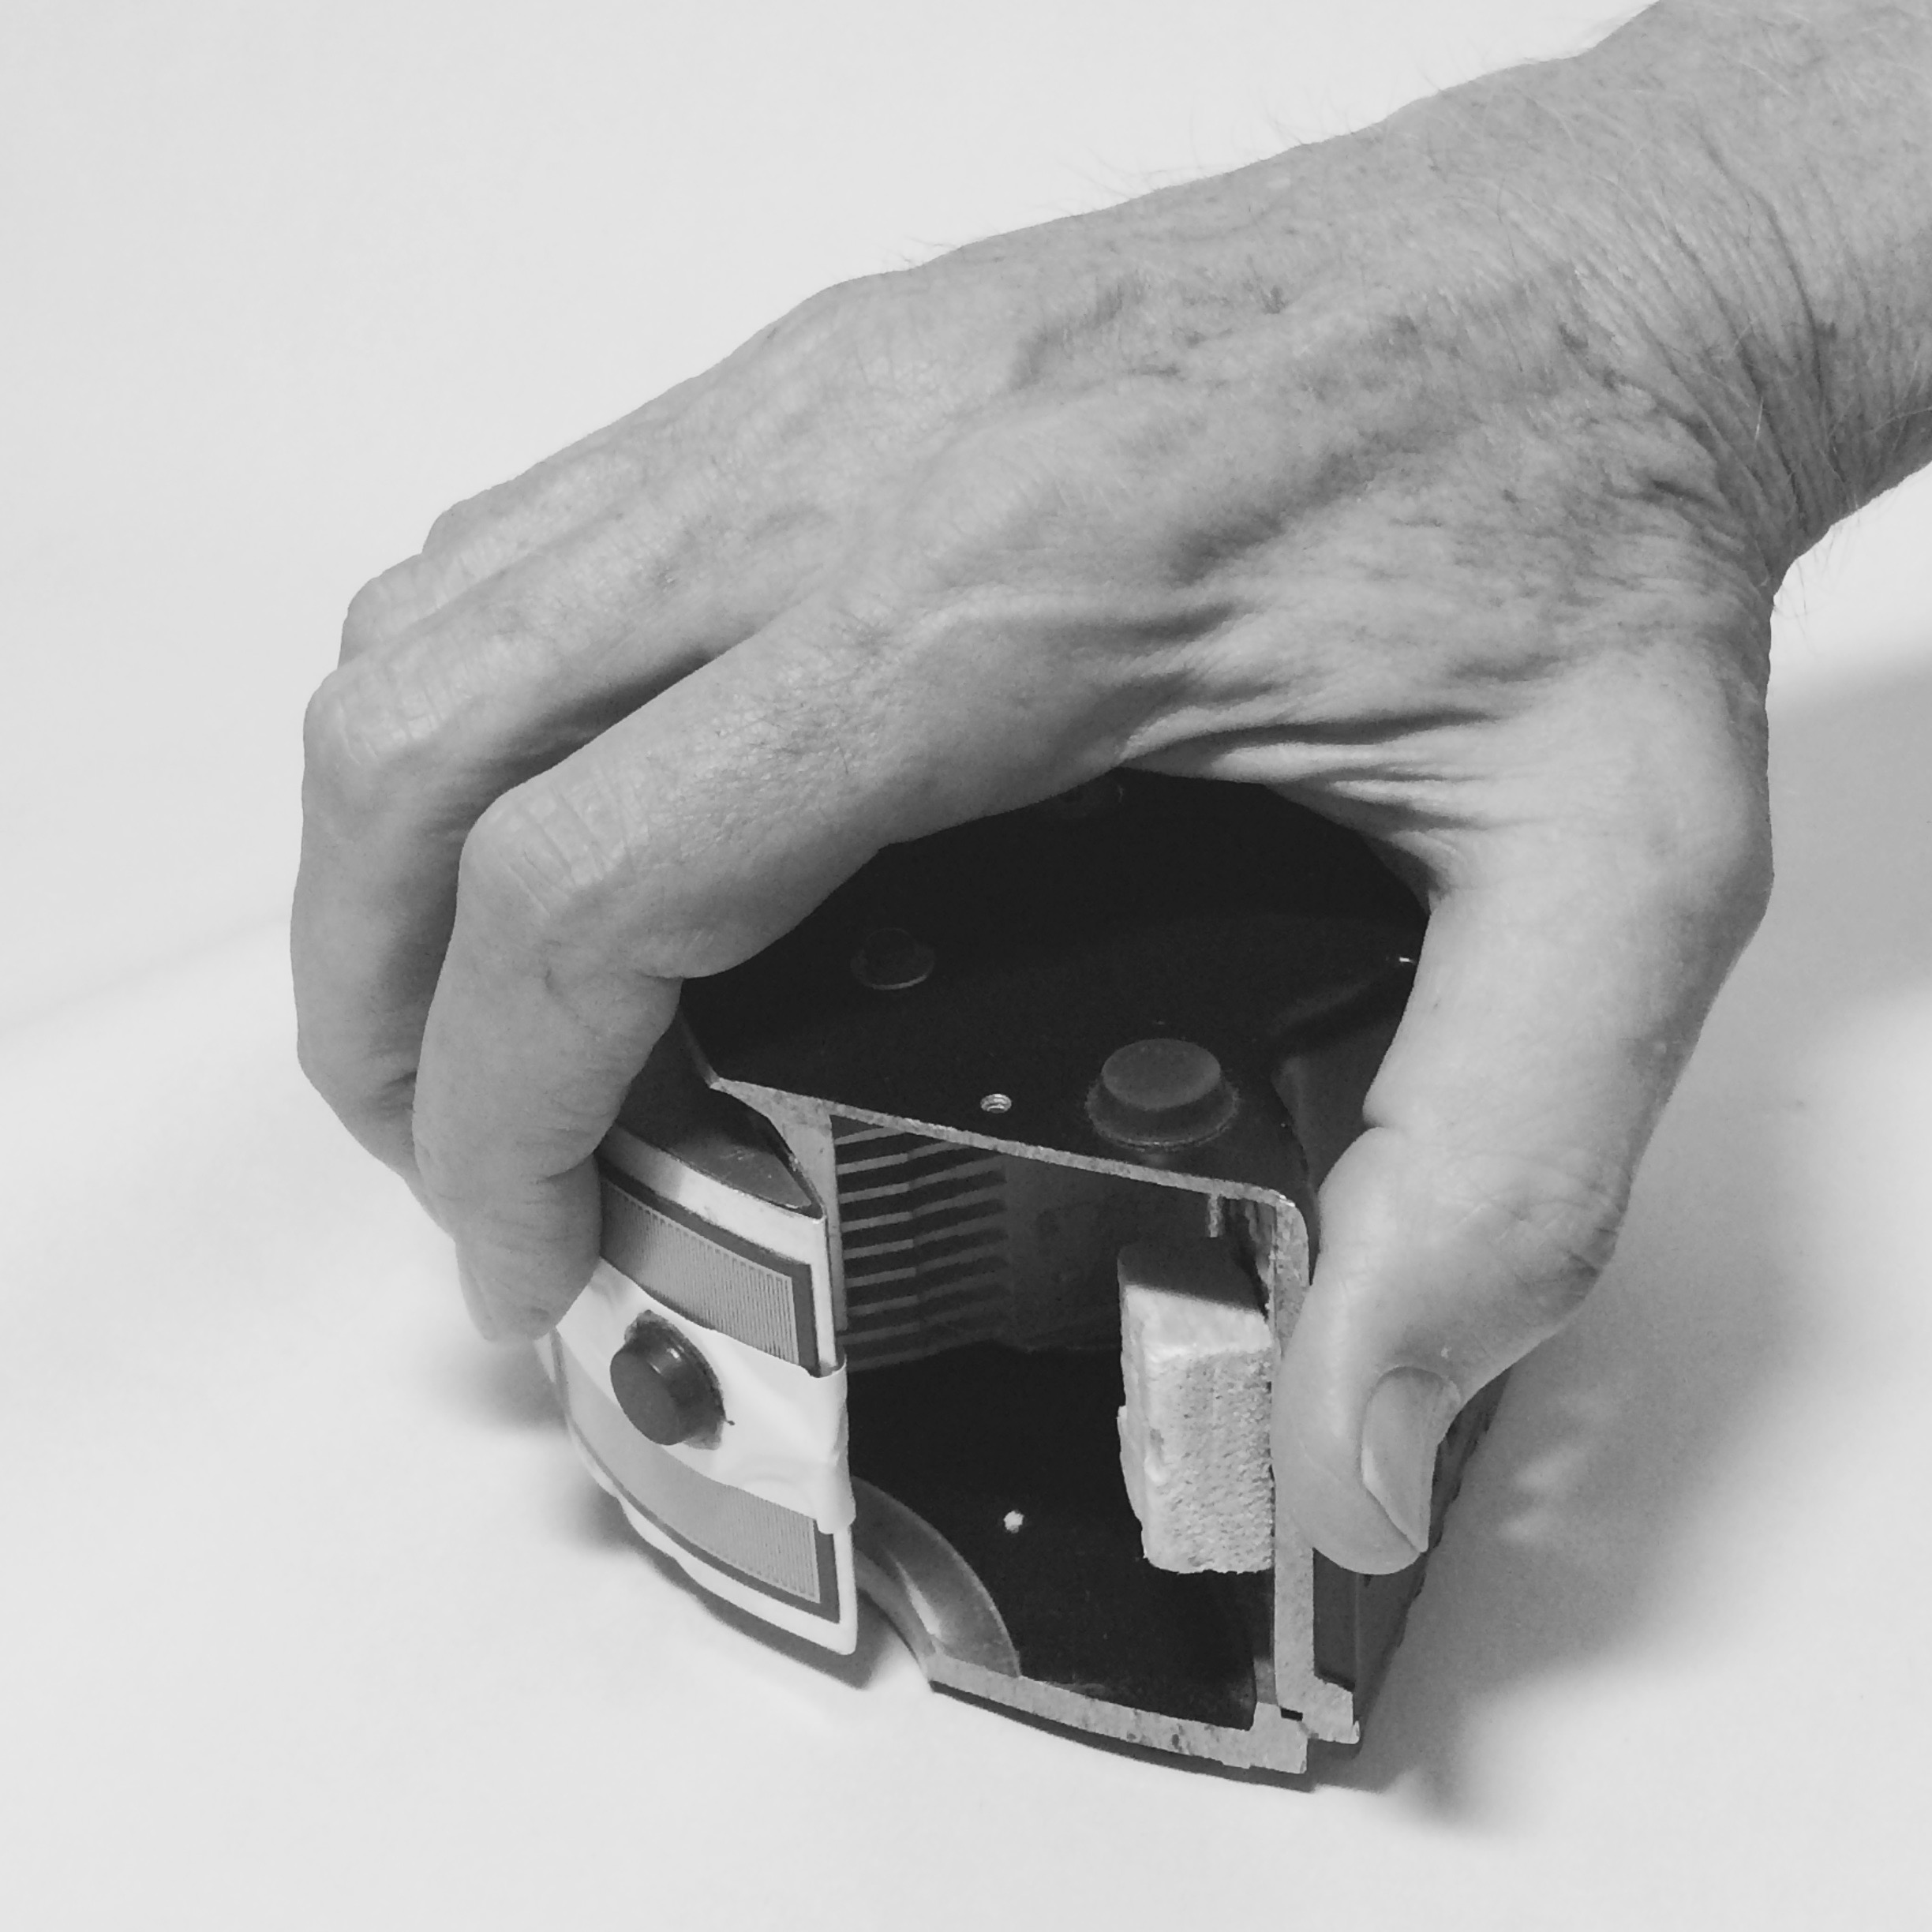
\includegraphics[width=3.85cm]{Plank7a}
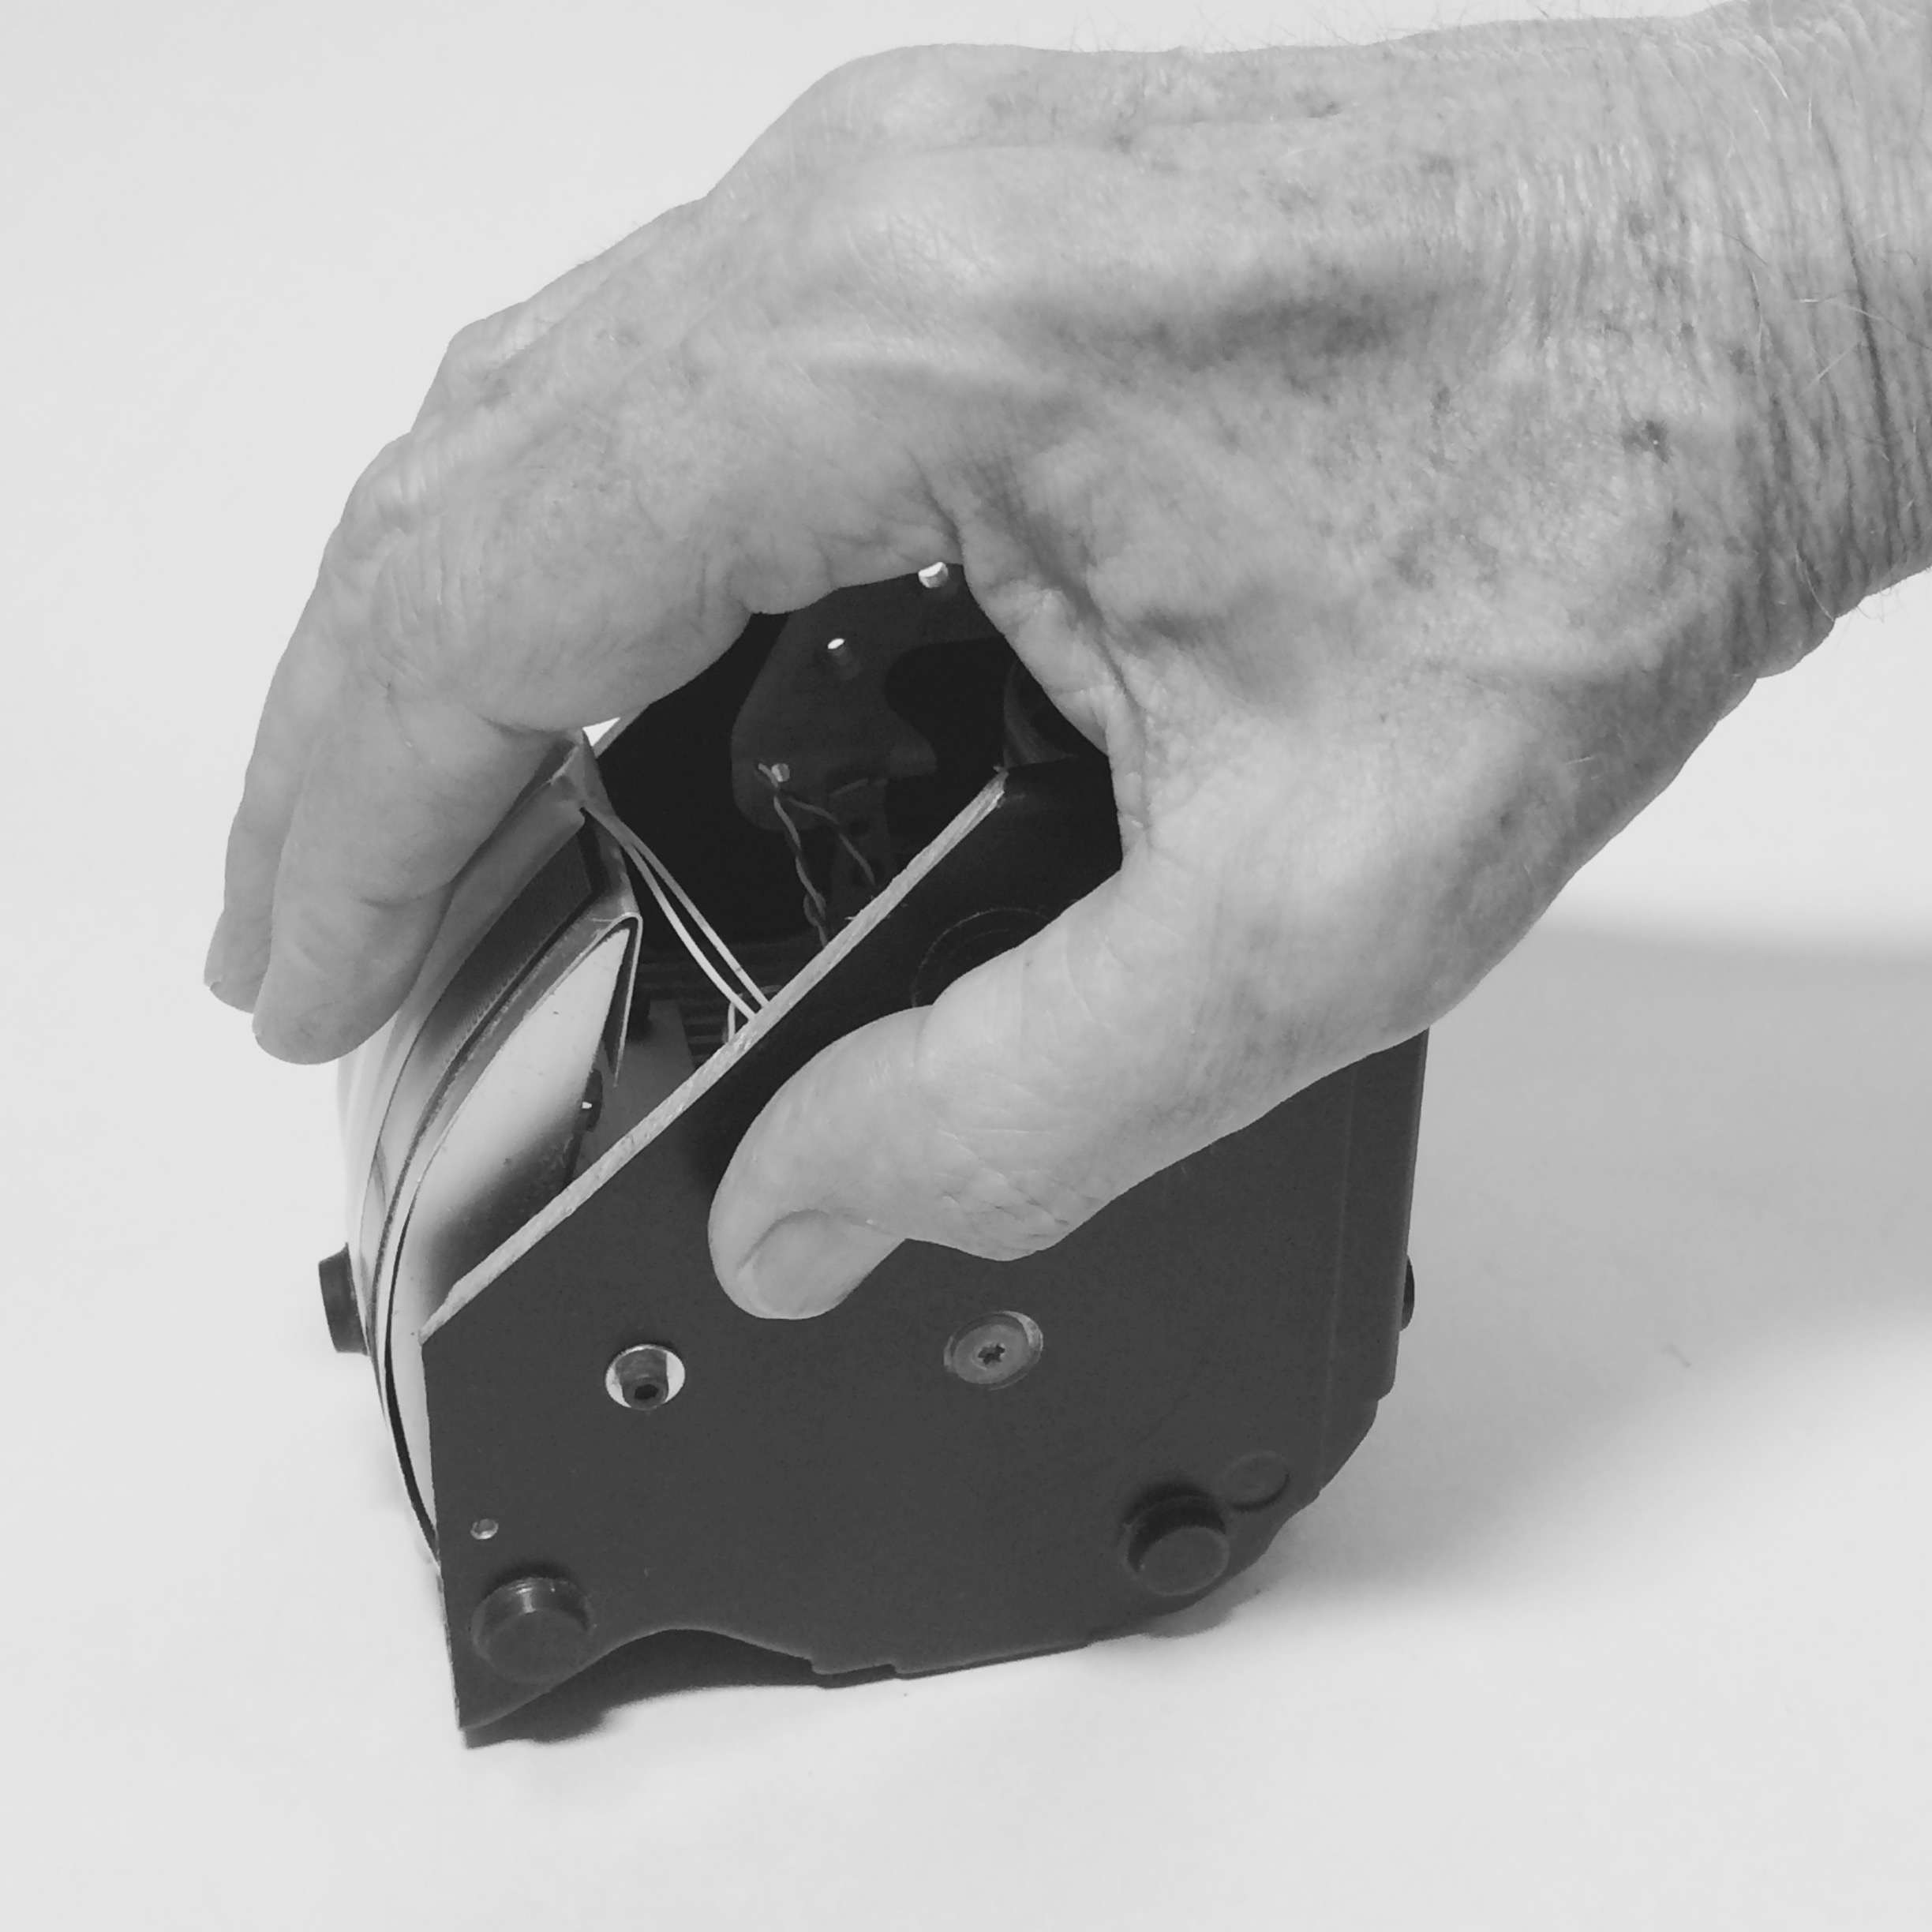
\includegraphics[width=3.85cm]{Plank7b}
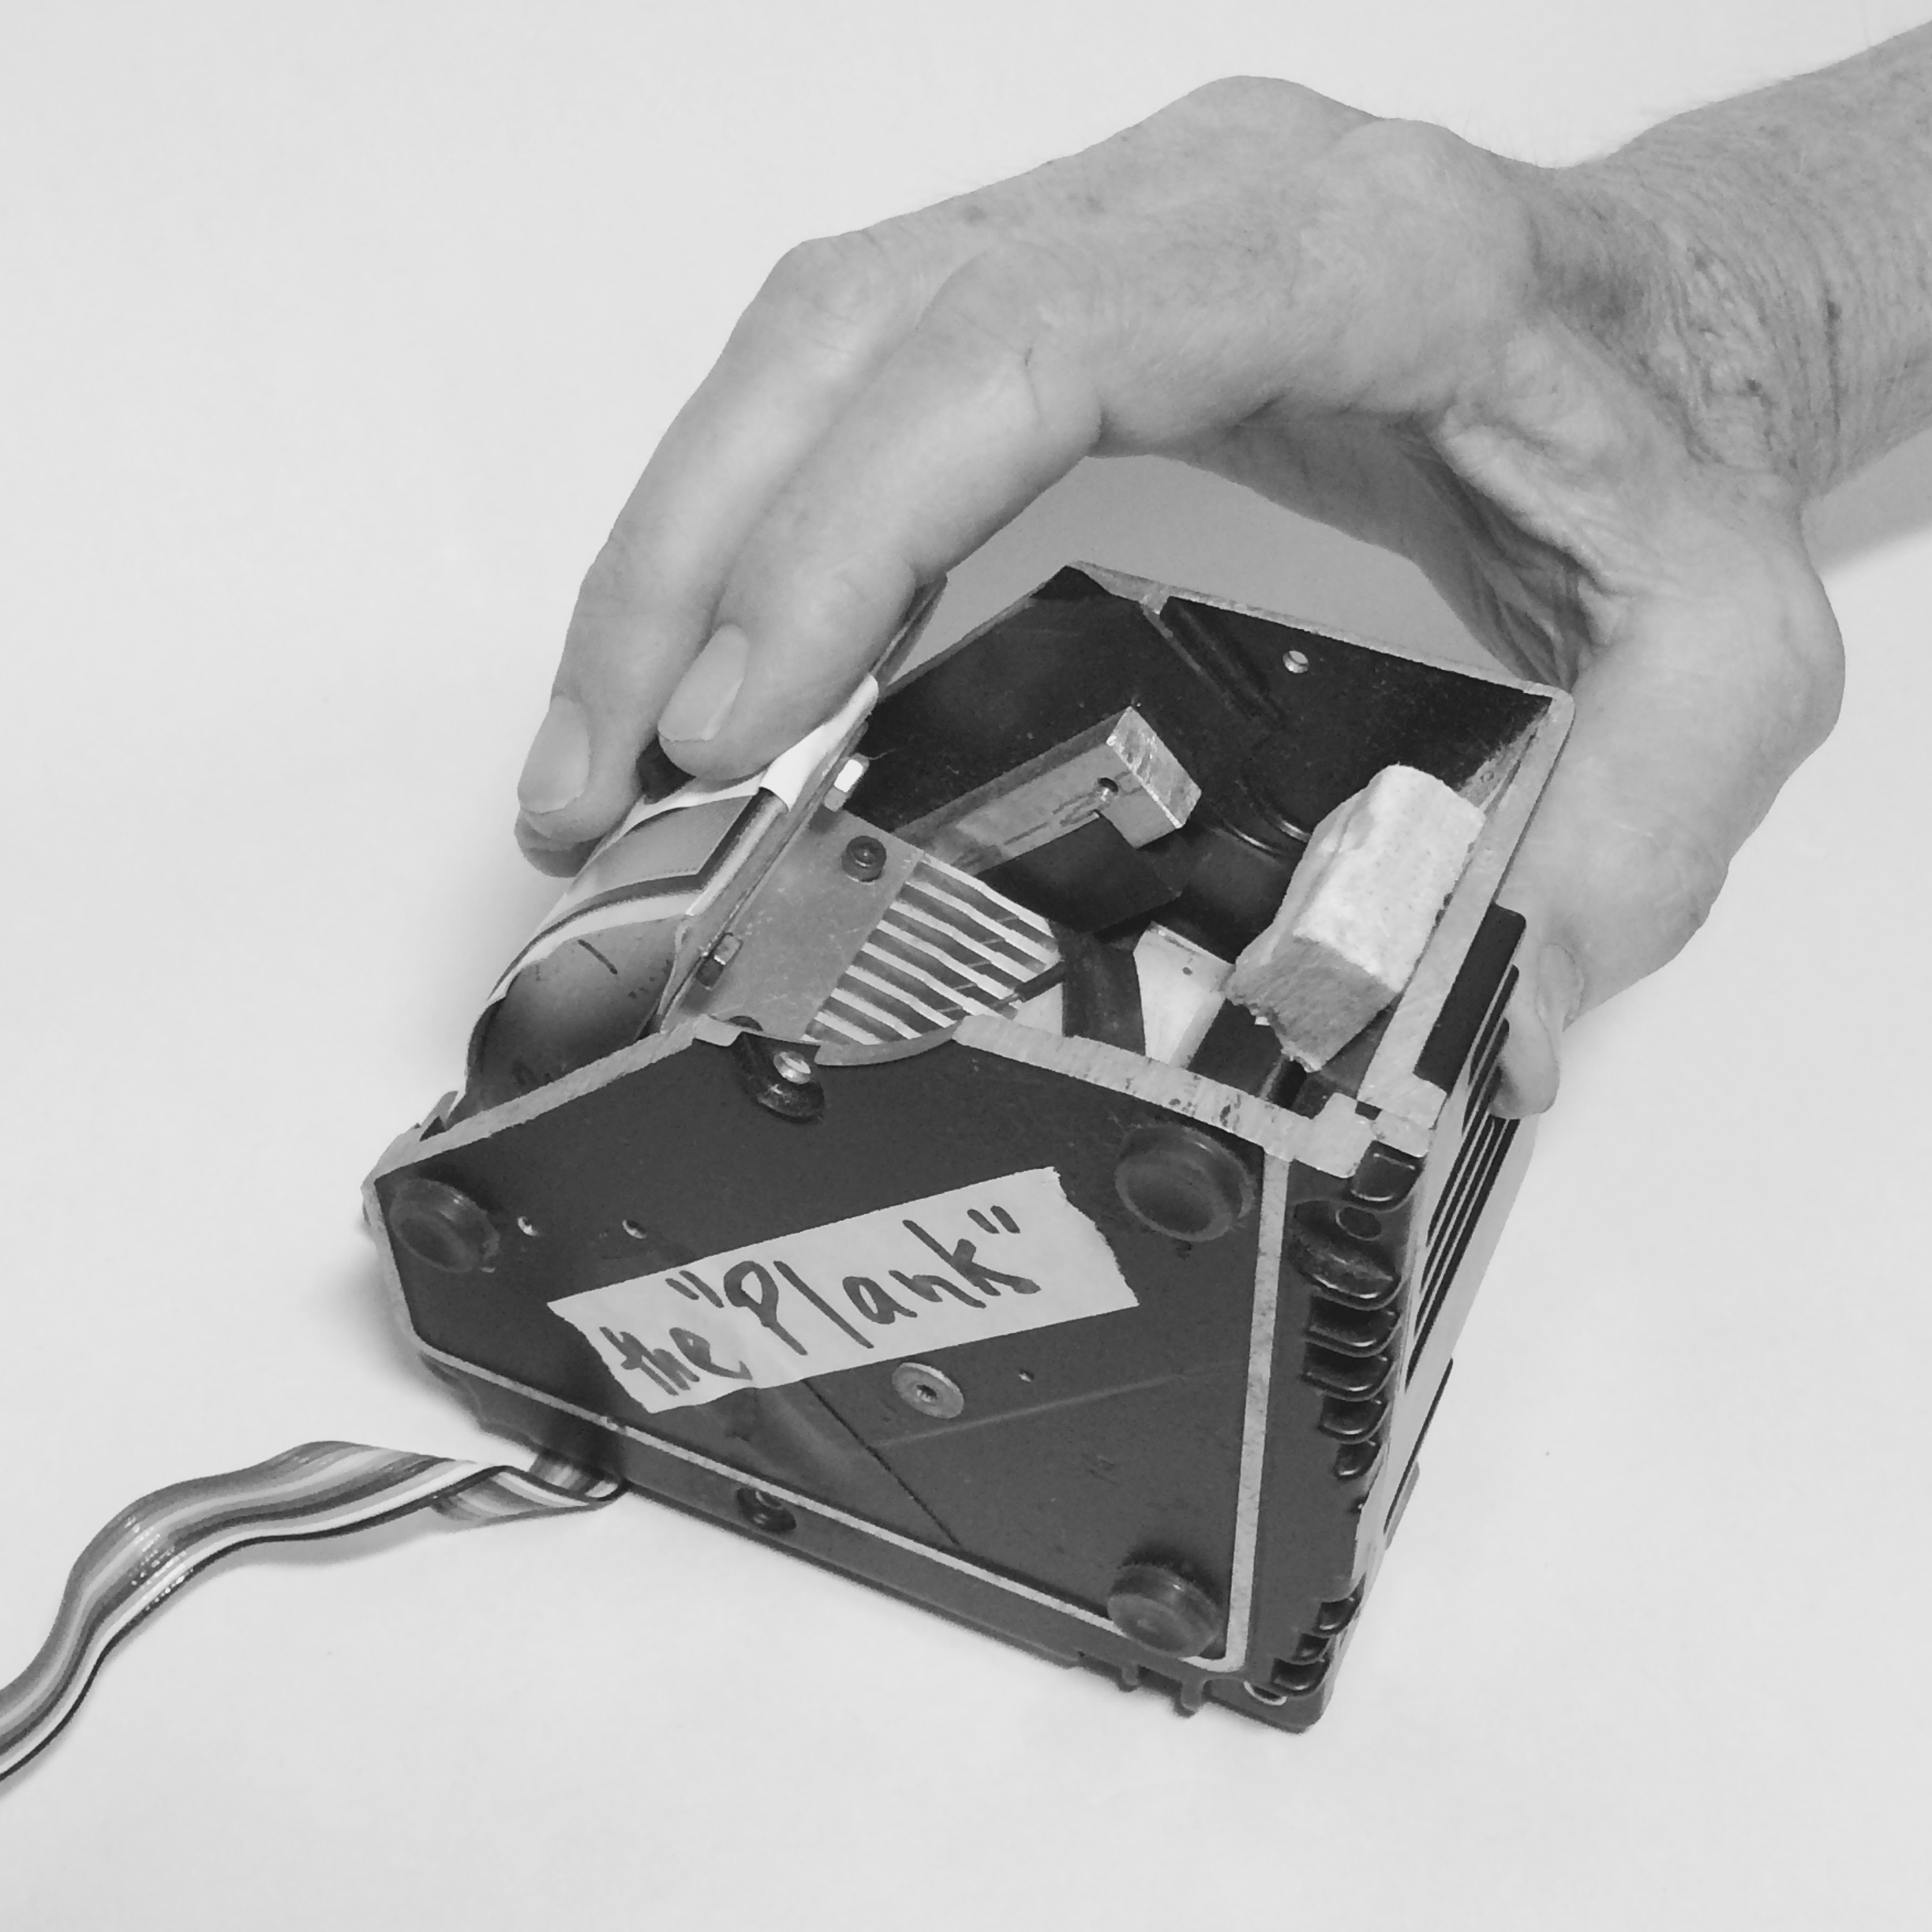
\includegraphics[width=3.85cm]{Plank7c}
\caption{Hand positions}
\label{Verplank:fig:7}       % Give a unique label
\end{figure}

\section{Progress and Plans}

The hardware and microprocessor software are working in a rough prototype. We are not yet communicating with the synthesizer let alone producing music. The Plank will be used to interface with scanned synthesis, and we will explore mappings of The Plank's interactions with wave terrains to audio parameters. An advantage of haptic interfaces for real-time music performance is that the performer now has another direct bidirectional interaction with the sound through his or her hands. We anticipate being able to simulate the feel of some traditional musical instruments (drums, piano, strings) allowing precise and fast control. We are also looking for new effects and unexpected, expressive sounds.

\begin{acknowledgement}
Interval Research supported six years of haptics research. Margaret Minsky, Brent Gillespie, Sile O'Modhrain, and in particular Karon Maclean inspired our work on simple devices. Rob Shaw showed us the magic of dynamics and helped invent scanned synthesis. Chris Chafe gave us a home at CCRMA.
\end{acknowledgement}

\section*{Author Commentary: Personal Reflections on The Plank}
\paragraph{Michael Gurevich and Bill Verplank}

The Plank was a direct outgrowth of research and experimentation by Verplank and Mathews at Interval Research that was in many ways a prototype for NIME itself: we were interested in developing new, interactive, audiovisual hardware/software technologies with primarily open-ended, creative applications.

The project can also be seen as an extension of Max Mathews' vision for computer music evident in his first real-time interactive computer music system---GROOVE---and ultimately of course in his Radio Baton. Max was an amateur violinist, but he didn't think the computer would make him a better musician. At Bell Labs, Max was among the pioneers to use the computer as a tool for simulation---initially to simulate telephone transmission systems; elaborating on this premise, he thought the computer could allow him (or anyone else) to simulate the experience of a great musician. Of course, there are many kinds of musical experiences, each of which is multi-faceted, and it ultimately occurred to Max and others that one aspect that was missing in many digital music systems was feel: the tactile, tangible relationship a performer has with their instrument; the ways an instrument pushes back on you when you push on it.

Others had certainly explored the intersection of haptics and music before The Plank. Brent Gillespie and Sile O'Modhrain preceded us at CCRMA \cite{Gillespie:1995}, and Claude Cadoz's group had been working on the problem since at least 1978 \cite{Cadoz:2003}. Charles Nichols presented his sophisticated haptic vBow at the same NIME (2002) as The Plank.  But in what we feel would become the essential spirit of NIME, and indeed the nascent ``Maker'' movement, The Plank sought to make haptics ``easy;'' the paper was really intended as a catalyst for others to try the same thing. It employed easily-obtainable, inexpensive, and largely open-source tools, and emphasized that the underlying principles could be implemented with little effort. 

It is worth noting that The Plank marked the first documented use in NIME of an Atmel AVR microcontroller (for which we owe an eternal debt of gratitude to Pascal Stang), which would become the core of the Arduino, now probably the most popular development board for physical computing in the world that powers much ``making'' and much of NIME.  As it turns out, this is no accident: Bill Verplank brought Pascal Stang's AVRmini development boards and AVRLib library (as well as The Plank) to the Interaction Design Institute Ivrea; when Massimo Banzi and others were frustrated they couldn't easily get their hands on more AVRmini boards, Arduino was born. 

One of the perpetual problems with experiential phenomena such as music is the difficulty in communication around the experience through the written medium. We are fortunate with music both to have a centuries-old discourse to draw upon, but also that it is relatively easy today to embed and distribute audio alongside or within written forums. We do not have either of these luxuries with haptics; for now, the best way to communicate about haptics, as well as to generate interest in musical haptics, is to ``feel it.'' For this reason, Verplank has remained committed to conducting courses and workshops on music and haptics, and to elaborating on making accessible tools like The Plank readily available. These efforts include a  ``Music \& Motors'' workshop that has run at the Copenhagen Institute of Interaction Design since 2011, which has produced numerous inventive projects, as well as a dedicated development board built on the Teensy 3.1 platform \cite{Bak:2015}. Several alumni of our workshops and courses have not only made substantial subsequent contributions at the intersection of music and haptics (e.g. \cite{Gillespie:1995}), but have also been responsible for expanding the incorporation of haptics into consumer products at companies including Apple and Immersion. 

Haptics remains a vital topic at NIME. Bill Verplank has continued to develop The Plank with a similar emphasis on helping to understand and emulate the ``feel'' of playing an acoustic instrument. Some of the most exciting work on haptics in NIME has come from Edgar Berdahl, who fulfilled one of our initial objectives for The Plank by creating a direct haptic interface to a computational acoustic simulation of a musical instrument---effectively unifying the haptic and sound synthesis models \cite{Berdahl:2009}. Berdahl has also expanded on O'Modhrain's work to examine ways that active force feedback may improve musicians' abilities to perform with digital and electroacoustic instruments \cite{Berdahl:2009a}. 

\section*{Expert Commentary: Haptics for Sonic Interaction Design using Recycled Motors}
\paragraph{Edgar Berdahl}

%\input{referenc}

Bill Verplank was a pioneer of NIME even before NIME became a recognized field. In the mid-1980s, he co-coined the term interaction design, and he helped introduce interaction design into digital musical practice by leading the NIME course at Stanford University for many years \cite{Berdahl:2013a}. He introduced valuable concepts to the NIME community such as distinguishing between musical ``buttons'' and musical ``handles,'' sketching and critiquing project ideas using his Interaction Design Framework, and designing haptic controls for music, which is the subject of this commentary.

In their seminal paper, Bill Verplank et al. described the first work on enabling students in a NIME course to experiment with haptic force-feedback controls. This work included the development of The Plank haptic device. The ingenuity of The Plank lies in the high-fidelity force feedback that a hard drive motor can provide (low inertia, low friction, relatively large peak torques) while concurrently emphasizing the value of recycling used electronics—due to the large number of mechanical hard drives discarded every year, these motors can be obtained at very low prices. Therefore, pedagogical exercises with The Plank not only inform about new sonic interactions enabled by force-feedback devices, but they also build connections with important ideas from found art and circuit bending \cite{Bak:2015,Ghazala:2005}. New technology is mass-produced by capitalist interests, yet haptic musical interactions can be enabled by recycling and rewiring old hard drive motors.

Although exercises with The Plank could convince students to think more holistically about recycling electronics and reducing waste, the process for creating Planks is somewhat daunting as it involves many steps. Consequently, other NIME researchers and musicians will likely prefer to obtain Planks directly from Bill Verplank himself, who has finely crafted the art of building them and distributes them via a series of open-source workshops. These workshops have been conducted in conjunction with Jakob Bak and David Gauthier. Their expanded series of haptic exercises emphasizes precise motor control via embedded programming using integers. Various schemes are employed for embellishing the firmware models with synthesized sound. Participants in these workshops have created an impressive array of beautiful project designs that point toward the future of haptics in NIMEs  \cite{Verplank:2001}.

These open-source workshops were preceded by my related work in open-source haptics, which has now culminated in the repository called Open Source Haptics for Artists. My work lies closer to computer music than to design. I aim to create software models for haptic control of high fidelity musical sound generated by floating-point algorithms. My personal goal is to create each model once, and then be able to render it using a wide array of future devices \cite{Hertz:2012}. In support of this goal, I focus on algorithm design and use embedded electronics only to interconnect haptic devices with powerful computational hardware.

In homage to the legacy established by Bill Verplank et al.'s work and vision, I am providing a way to connect The Plank with the Open Source Haptics for Artists repository.\footnote{\url{https://github.com/eberdahl/Open-Source-Haptics-For-Artists/tree/master/Hardware/ThePlank}} This is most easily accomplished with a capacitive sensor, which can be implemented by soldering a wire to a piece of copper tape, using double-stick tape to fix the copper tape against the backside of The Plank handle, and then connecting this wire to the FireFader microcontroller board. Then, any of the models developed for my open-source FireFader device can also be rendered using The Plank.

Overall, the mechanical performance of The Plank is very good. However, according to my informal tests, the position sensor is noticeably nonlinear, yet it is monotonic and close enough to linear that most of my models produce the desired result if sometimes with a slightly warped perspective.

One of my models contains a series of force profiles that can be customized by the user drawing into a table with the mouse. The force profile concept is described in Bill Verplank et al.'s featured original paper, and the equation below describes the physical relationship mathematically. The height $h(x)$ of a virtual mass $m$ on a frictionless terrain at position $x$ can be related to the force profile $F(x)$ by way of an integral:

\begin{equation}
\mathrm{Work} = -\int_0^x F(x_m)dx_m = mg\Big(h(x)-h(0)\Big).
\end{equation}

In closing, it is hoped that open-source haptics will continue to flourish within the community and enable Bill Verplank's goal---that NIME community members have the access and knowledge to tastefully incorporate haptic force-feedback control into their projects.  The greater the depth and breadth of open-source resources, the more new possibilities are enabled.


\graphicspath{ {mainmatter/Blaine_2003/} }

\title*{2003: Contexts of Collaborative Musical Experiences}
\titlerunning{Contexts of Collaborative Musical Experiences}


\author{Tina Blaine and Sidney Fels}
\authorrunning{Blaine and Fels}

%\institute{Tina Blaine \at CMU Entertainment Technology Center, Rhythmix Cultural Works, Alameda, CA 94501,\email{tblaine@gmail.com}
%\and  Sidney Fels \at  Dept. of Electrical Computer Engineering, University of British Columbia,Vancouver, BC, V6T 1Z4, \email{ssfels@ece.ubc.ca}}

%
%
\maketitle

\abstract*{We explore a variety of design criteria applicable to the creation of collaborative interfaces for musical experience. The main factor common to the design of most collaborative interfaces for novices is that musical control is highly restricted, which makes it possible to easily learn and participate in the collective experience. Balancing this trade-off is a key concern for designers, as this happens at the expense of providing an upward path to virtuosity with the interface. We attempt to identify design considerations exemplified by a sampling of recent collaborative devices primarily oriented toward novice interplay. It is our intention to provide a non-technical overview of design issues inherent in configuring multiplayer experiences, particularly for entry-level players.}

\section{Introduction}

The emergence of electronic instruments, and most notably the computer, has led
to the creation of new interfaces and sounds never before possible.  In addition,
the computer can be used to create arbitrary mappings between gesture and sound,
thereby providing the possibility of computer-supported sound and directed
musical interaction. Consequently, a wave of new types of collaborative
interfaces and group experiences has emerged for collective music making with the
potential to include people with little or no musical training. Therefore,
understanding the role of music in relation to people's experiences playing
collaborative instruments requires a shift in perspective.  By attributing less
relevance to the importance of traditional music metrics based on melody, more
emphasis can be placed on metrics that involve the players' experience. The
psychological state of ``flow'' is achieved by engaging in deeply satisfying
experiences that alter one's state of consciousness \cite{Csikszentmihalyi:1990}. Making collaborative
interfaces relatively simple and easy to learn facilitates flow for novices. This
approach can also support the development of intimacy with the interface, which
has an ``aesthetic of control'' \cite{Fels:2000}. When designing collaborative musical
experiences for first-time players in public places, the amount of time necessary
to learn an interface must be minimized, coupled with achieving a balance between
virtuosity and simplicity \cite{DArcangelo:2001}.  Providing an upward path of increasing complexity
necessary for maintaining flow, while at the same time providing an entry level
low enough for novices, is very challenging and continues to necessitate further
inquiry by experience designers.

\subsection{Accessible Music}

The underlying premise of most collaborative interface design is that with
various design constraints, playing music can be made accessible to
non-musicians. Participation in making music gives players a sense of belonging
and access to a new community at the expense of limiting the musical range and
possible gestures associated with sound in a collective space. We suggest that
analyzing the musical experience of collaborative interfaces should be examined
in this context. Essentially, low-level accessibility is necessary for people to
participate and communicate with the instruments and each other.  Furthermore,
many collaborative interfaces are intended for public exhibition, where people
casually ``walk-up and play.''  This restricts the amount of time that a designer
can expect someone to spend learning an interface, and necessitates highly
constrained interfaces that are conducive to easily accessible musical
experiences.

Therefore, we suggest that providing novices with easily accessible music making
experiences is more important than having a complex interface with built-in,
upward capability for virtuosic expression. The counter-argument to this
assumption is that a low entry fee should have no ceiling on virtuosity \cite{Wessel:2001}.
Wessel and Wright posit that ``\ldots{}many of the simple-to-use computer
interfaces proposed for musical control seem, after even a brief period of use,
to have a toy-like character and do not invite continued musical evolution'' \cite{Wessel:2001}. 
While this is fundamentally true for expert musicians, the main opposition to
this viewpoint regarding novice interplay is that the demographic for most
multiplayer instruments are non-musicians and accordingly, the same principles do
not necessarily apply.  Although expert musicians are concerned with expressive
capabilities and mastery of their instruments, it is unlikely that first time
players have the expectation of becoming expert players on any musical
instrument.

\subsection{Balancing Complexity and Expressivity }

The trade-off in determining the appropriate balance of complexity and
expressivity of an interface is not easily resolved.  Historically, the field of
musical controllers has advanced primarily through the creation of highly complex
single player instruments developed for experts, as opposed to multiplayer
interfaces/environments designed for novices \cite{Cutler:2000,Paradiso:1997a}. Developing musical
interfaces using familiar objects that ordinarily serve another purpose, or
inventing entirely new instruments, can change the level of musical expectation
by redefining ``expert'' and ``novice'' interplay as the basis for engagement.
``Playful'' interfaces can also avoid the look and feel of traditional instruments
 \cite{Cook:2001}.  Designers of collaborative devices that are easy to control but have
limited expressive capabilities are challenged not only to conceive of
opportunities for musical exploration, but must also cultivate meaningful social
interactions and experiences for the players. In a collaborative musical
environment, it becomes even more imperative that the technology serves primarily
as a catalyst for social interaction, rather than as the focus of the experience
 \cite{Robson:2001}. Conversely, interfaces that have extended expressive capabilities tend to be
more difficult to control and cater more to the expert player. For designers of
most musical interfaces, the overriding challenge is to strike a balance of
multimodal interaction using discrete and continuous controls \cite{Tanaka:2002}, \cite{Verplank:2001}, and
generally, limit rather than increase the number of features and opportunities
for creativity \cite{Cook:2001}.

\subsection{Mapping and Control Issues }

Natural mapping behaviors evolve from the creation of a
direct relationship between gesture and musical intent. Players' perception of
control in collaborative musical environments can be increased by creating
predetermined musical events, subject to players manipulating complex parameters
of sound through gestures, such as stretching or squeezing \cite{Weinberg:2001}. Enhancing the
illusion of control can also be achieved with supplemental effects such as
lighting, visual imagery and more, to create a highly responsive system based on
player input.  While the use of pre-composed musical events or sequences severely
limits certain aspects of an individual's creative control, it has the benefit of
creating more cohesive sound spaces in multiplayer environments. With these
mappings, players are not responsible for playing specific notes, scales or
harmonies, which helps to minimize chaotic musical interaction.

\section{Contexts of Collaborative Interfaces}

Collaborative musical interfaces may be roughly classified by a number of
different attributes unique to the context of communal experience. Table~\ref{blaine-tab:1}
provides a sample listing of multiplayer systems organized by the following
elements of design: \textit{Focus}, \textit{Location}, \textit{Media},
\textit{Scalability}, \textit{Player} \textit{Interaction}, \textit{Musical
Range}, \textit{Physical Interface}, \textit{Directed Interaction},
\textit{Pathway to Expert Performance} and \textit{Level of Physicality}.

Design issues regarding the input interface, input-to-output mapping and the
output interface are of the utmost relevance as well as the topic of much
research.\footnote{Organised Sound special issue on mappings and the New
Interfaces for Musical Expression (NIME) proceedings all address these design
issues.} Thus, the type of collaborative interface depends on a number of factors
including range, sensor(s), directed interaction, and pathway to expert
performance.  Good design practice for these instruments, whether cooperative or
not, overlaps with issues regarding human-computer interaction \cite{Orio:2001}. Such issues
include usability, ease of learning, and functionality, specifically in relation
to their effects on the success of the \textit{collaborative} experience. Finding
the balance between virtuosity and simplicity provides fertile ground for new
collaborative interfaces.  Due to space constraints, the authors were unable to
include a more comprehensive list, or technical discussion regarding the systems
referenced herein.

\subsection{Focus}

The focus of the experience is determined by establishing whether the
communication is primarily between players or between players and an audience.
Collaborative instruments are usually designed to enhance the communicative
experience between players rather than exploit virtuosic play for the benefit of
an audience. This may or may not be very interesting for an audience to listen
to, since they are not privy to the subtleties of interaction that occurs between
players. Most computer-based instruments do not provide direct means for
audiences to see how players' gestures affect the music and instead must rely
upon indirect means, such as explanation of the interaction or visualization.

\subsection{Location}

Many collaborative interfaces for musical expression are created as
installations for public exhibition.  In these instances, people are often
expected to converge at a specific location and/or gather around an instrument to
play together.  Because they are co-located, players can see each other's
gestures and more readily understand the relationship between each player's
actions and the sounds produced. However, if the sounds are not easily
attributable to specific actions or devices, then players must find other ways to
communicate.  \textit{Beatbugs }  \cite{Weinberg:2002a}, \textit{Musical Trinkets } \cite{Paradiso:2001},
and\textit{ SoundMapping} \cite{Mott:1997},  all work around this issue in a variety of ways.
 With the growth of the Internet, a new genre of collaborative interfaces allows
players to communicate over a network from non-specific locations, from virtually
anywhere in the world \cite{Weinberg:2002}.  Systems such as the \textit{Hub} \cite{Gresham-Lancaster:1998}, \textit{Brain
Opera} \cite{Machover:1996,Paradiso:1999},\textit{ Faust Music OnLine} (FMOL) \cite{Jorda:1999}, and \textit{Rocket
Network} \cite{Hall:2002}, are notable examples of efforts in this direction that
integrate(d) more professional levels of musicianship.

\subsection{Media}

Many collaborative interfaces combine audiovisual elements as a way of enhancing
communication and creating more meaningful experiences. The use of visual imagery
can facilitate the collaborative experience by reinforcing the responsiveness of
the system to players' actions.  However, visual imagery can also distract
players from seeing other players' actions, or from attending to aural elements,
or both. Some of the systems that include visual imagery as the primary medium
include \textit{Jamoworld } \cite{Blaine:2002}, \textit{Jamodrum} \cite{Blaine:2000}, \textit{Iamascope} \cite{Fels:1999},
and \textit{Currents of Creativity} \cite{DArcangelo:2001}. One particular challenge with visually
oriented systems, is that the identification of players with imagery can be so
strong that the act of making music becomes a secondary part of the experience.

\subsection{Scalability}

By their very nature, collaborative interfaces are designed for a minimum of two
or more players.  However, the number of players greatly influences the types of
interfaces and music that is appropriate.  An interface built for two people is
generally quite different from one built for tens, hundreds or thousands of
players. When considering scale, factors such as turn-taking protocols and
gesture-sound correspondences shift as the number of players increase.  For
example, it does not make sense to expect turn-taking protocols to emerge in an
interface with three hundred drum pad inputs distributed through a large area, as
embedded in the \textit{RhythmTree} structure \cite{Paradiso:1999}.  Directly refuting this
notion is the \textit{MidiBall} \cite{Jacobson:1993} interface, where only a few people are
physically able to hit the ball at one time, even if hundreds or thousands of
people are present.

\subsection{Player Interaction}

Generally, collaborative instruments provide each player with a method for
individual control within a shared sonic environment.  Although the control
devices may be identical or different for each player, the underlying method of
interaction is quite often the same.  For example, in \textit{Musical Trinkets}
 \cite{Paradiso:2001} and Musical Navigatrics \cite{Pardue:2002}, each player has their own unique set of
figures used to control sound.  While each trinket has a specific sound or
algorithmic effect associated with it, all players interact in the same way, by
moving the objects over a shared tabletop surface in order to activate those
sounds. In a communal space without too many people and/or distractions, this
approach has the advantage that players are able to observe each other to
determine what distinguishes each player's visual and aural impact.  However, if
the mapping between the interface or device and its affect on the sonic output is
unclear, then it becomes more difficult to use the interface for musical
collaboration.


%
% Note to Publisher: the following large table does not fit the template very well. This will require
% attention of an expert to find a solution for formatting the table, which is essential to this article.
%

\begin{center}

\begin{table}[ht]
\label{blaine-tab:1}
\caption{Contexts of Collaborative Interface Design}
\vspace{3pt} \noindent
\begin{tabular}{|p{41pt}|p{22pt}|p{22pt}|p{26pt}|p{17pt}|p{26pt}|p{31pt}|p{35pt}|p{33pt}|p{24pt}|p{35pt}|p{26pt}|p{36pt}|}
\hline
\parbox{41pt}{\centering 
\textbf{{\small System}}
} & \parbox{22pt}{\centering 
\textbf{{\small Focus}}
} & \parbox{22pt}{\centering 
\textbf{{\small Location}}
} & \parbox{26pt}{\centering 
\textbf{{\small Media}}
} & \parbox{17pt}{\centering 
\textbf{{\small Scale}}
} & \parbox{26pt}{\centering 
\textbf{{\small Player  Inter-action}}
} & \parbox{31pt}{\centering 
\textbf{{\small Musical Range/}}

\textbf{{\small Notes}}
} & \parbox{35pt}{\centering 
\textbf{{\small Physical Interface/Sensor}}
} & \parbox{33pt}{\centering 
\textbf{{\small Directed Inter-action}}
} & \parbox{24pt}{\centering 
\textbf{{\small Learning Curve}}
} & \parbox{35pt}{\centering 
\textbf{{\small Pathway to Expert Perform-ance}}
} & \parbox{26pt}{\centering 
\textbf{{\small Level of Physical-ity}}
} & \parbox{36pt}{\centering 
\textbf{{\small Musical Genre}}
} \\
\hline
\parbox{41pt}{\raggedright 
{\small \textbf{Audio Grove} (Moeller, 1997)}
} & \parbox{22pt}{\raggedright 
{\small Players}
} & \parbox{22pt}{\raggedright 
{\small Local}
} & \parbox{26pt}{\raggedright 
{\small Sound, Light, Device}
} & \parbox{17pt}{\raggedright 
{\small 1--30  }
} & \parbox{26pt}{\raggedright 
{\small Same}
} & \parbox{31pt}{\centering 
{\small Players control DSP}
} & \parbox{35pt}{\centering 
{\small Touch, Capacitive sensing}
} & \parbox{33pt}{\centering 
{\small Low}
} & \parbox{24pt}{\centering 
{\small Fast}
} & \parbox{35pt}{\centering 
{\small No}
} & \parbox{26pt}{\centering 
{\small High}
} & \parbox{36pt}{\raggedright 
{\small Ambient}
} \\
\hline
\parbox{41pt}{\raggedright 
{\small \textbf{Augmented Groove} \cite{Poupyrev:2001}}
} & \parbox{22pt}{\raggedright 
{\small Players}
} & \parbox{22pt}{\raggedright 
{\small Local}
} & \parbox{26pt}{\raggedright 
{\small Sound, Image, Device}
} & \parbox{17pt}{\raggedright 
{\small 1--3}
} & \parbox{26pt}{\raggedright 
{\small Same}
} & \parbox{31pt}{\centering 
{\small Players control DSP}
} & \parbox{35pt}{\centering 
{\small Camera, HMD, Glyph Disks}
} & \parbox{33pt}{\centering 
{\small Med-High facilitator}
} & \parbox{24pt}{\centering 
{\small Med-Fast}
} & \parbox{35pt}{\centering 
{\small No}
} & \parbox{26pt}{\centering 
{\small High}
} & \parbox{36pt}{\raggedright 
{\small Techno, House}
} \\
\hline
\parbox{41pt}{\raggedright 
{\small \textbf{Beatbugs }(Weinberg et al., 2002)}
} & \parbox{22pt}{\raggedright 
{\small Players+ Aud-ience}
} & \parbox{22pt}{\raggedright 
{\small Local}
} & \parbox{26pt}{\raggedright 
{\small Sound, Device}
} & \parbox{17pt}{\raggedright 
{\small 1--8}
} & \parbox{26pt}{\raggedright 
{\small Same}
} & \parbox{31pt}{\centering 
{\small Players control DSP + rhythmic input}
} & \parbox{35pt}{\centering 
{\small InfraRed, Bend sensors, Piezos}
} & \parbox{33pt}{\centering 
{\small High workshops+ dist'd leadership}
} & \parbox{24pt}{\centering 
{\small Slow}
} & \parbox{35pt}{\centering 
{\small Possibly}
} & \parbox{26pt}{\centering 
{\small High}
} & \parbox{36pt}{\raggedright 
{\small Electronic Poly-rhythmic}
} \\
\hline
\parbox{41pt}{\raggedright 
{\small \textbf{Brain Opera} (Machover, 1996)}
} & \parbox{22pt}{\raggedright 
{\small Players + Aud-ience}
} & \parbox{22pt}{\raggedright 
{\small Local and Net}
} & \parbox{26pt}{\raggedright 
{\small Sound, Image, Device}
} & \parbox{17pt}{\raggedright 
{\small 1--100's}
} & \parbox{26pt}{\raggedright 
{\small Differ-ent}
} & \parbox{31pt}{\centering 
{\small Limited \& Unlimited}
} & \parbox{35pt}{\centering 
{\small Varied Custom Devices}
} & \parbox{33pt}{\centering 
{\small Conductor, facilitators + freeplay}
} & \parbox{24pt}{\centering 
{\small Slow--Fast}
} & \parbox{35pt}{\centering 
{\small Possibly}
} & \parbox{26pt}{\centering 
{\small Med--High}
} & \parbox{36pt}{\raggedright 
{\small Varied}
} \\
\hline
\parbox{41pt}{\raggedright 
{\small \textbf{Bullroarer }(Robson, 2001)}
} & \parbox{22pt}{\raggedright 
{\small Players}
} & \parbox{22pt}{\raggedright 
{\small Local}
} & \parbox{26pt}{\raggedright 
{\small Sound, Device}
} & \parbox{17pt}{\raggedright 
{\small 1--3}
} & \parbox{26pt}{\raggedright 
{\small Same}
} & \parbox{31pt}{\centering 
{\small Players control DSP}
} & \parbox{35pt}{\centering 
{\small Sliders, potentio-meters}
} & \parbox{33pt}{\centering 
{\small Low}
} & \parbox{24pt}{\centering 
{\small Fast}
} & \parbox{35pt}{\centering 
{\small No}
} & \parbox{26pt}{\centering 
{\small High}
} & \parbox{36pt}{\raggedright 
{\small Ambient Drones, Electronic }
} \\
\hline
\parbox{41pt}{\raggedright 
{\small \textbf{Composition on the Table} (Iwai, 1998)}
} & \parbox{22pt}{\raggedright 
{\small Players}
} & \parbox{22pt}{\raggedright 
{\small Local}
} & \parbox{26pt}{\raggedright 
{\small Image, Sound, Light, Device}
} & \parbox{17pt}{\raggedright 
{\small 1--6}
} & \parbox{26pt}{\raggedright 
{\small Same}
} & \parbox{31pt}{\centering 
{\small Players control rhythm + midi loops}
} & \parbox{35pt}{\centering 
{\small Buttons, Switches, Faders}
} & \parbox{33pt}{\centering 
{\small Low}
} & \parbox{24pt}{\centering 
{\small Fast}
} & \parbox{35pt}{\centering 
{\small No}
} & \parbox{26pt}{\centering 
{\small Med}
} & \parbox{36pt}{\raggedright 
{\small Minimalist }
} \\
\hline
\parbox{41pt}{\raggedright 
{\small \textbf{Currents of Creativity} (D'Arcangelo, 2001)}
} & \parbox{22pt}{\raggedright 
{\small Players}
} & \parbox{22pt}{\raggedright 
{\small Local}
} & \parbox{26pt}{\raggedright 
{\small Image, Sound, Device}
} & \parbox{17pt}{\raggedright 
{\small 1--6}
} & \parbox{26pt}{\raggedright 
{\small Same}
} & \parbox{31pt}{\centering 
{\small Limited: pre-composed loops}
} & \parbox{35pt}{\centering 
{\small Computer Kiosk}
} & \parbox{33pt}{\centering 
{\small High}
} & \parbox{24pt}{\centering 
{\small Fast}
} & \parbox{35pt}{\centering 
{\small No}
} & \parbox{26pt}{\centering 
{\small Med}
} & \parbox{36pt}{\raggedright 
{\small World}
} \\
\hline
\parbox{41pt}{\raggedright 
{\small \textbf{FMOL }(Jorda, 1999)}
} & \parbox{22pt}{\raggedright 
{\small Players}
} & \parbox{22pt}{\raggedright 
{\small Net}
} & \parbox{26pt}{\raggedright 
{\small Sound, Image, Software}
} & \parbox{17pt}{\raggedright 
{\small 2}
} & \parbox{26pt}{\raggedright 
{\small Same}
} & \parbox{31pt}{\centering 
{\small Unlimited}
} & \parbox{35pt}{\centering 
{\small Mouse, Kybd}
} & \parbox{33pt}{\centering 
{\small No}
} & \parbox{24pt}{\centering 
{\small Medium}
} & \parbox{35pt}{\centering 
{\small Yes}
} & \parbox{26pt}{\centering 
{\small Low}
} & \parbox{36pt}{\raggedright 
{\small Electronic}
} \\
\hline
\parbox{41pt}{\raggedright 
{\small \textbf{Hub }(Gresham-Lancaster, 1998)}
} & \parbox{22pt}{\raggedright 
{\small Aud-ience}
} & \parbox{22pt}{\raggedright 
{\small Local and Net}
} & \parbox{26pt}{\raggedright 
{\small Sound, Soft-ware}
} & \parbox{17pt}{\raggedright 
{\small 1--6}
} & \parbox{26pt}{\raggedright 
{\small Differ-ent}
} & \parbox{31pt}{\centering 
{\small Unlimited}
} & \parbox{35pt}{\centering 
{\small Mouse, Keyboard, Joysticks Trackball + MIDI Devices}
} & \parbox{33pt}{\centering 
{\small No}
} & \parbox{24pt}{\centering 
{\small Slow}
} & \parbox{35pt}{\centering 
{\small Yes}
} & \parbox{26pt}{\centering 
{\small Low}
} & \parbox{36pt}{\raggedright 
{\small Electronic}
} \\
\hline
\parbox{41pt}{\raggedright 
{\small \textbf{Iamascope }(Fels and Mase, 1998)}
} & \parbox{22pt}{\raggedright 
{\small Players}
} & \parbox{22pt}{\raggedright 
{\small Local}
} & \parbox{26pt}{\raggedright 
{\small Image, Sound}
} & \parbox{17pt}{\raggedright 
{\small 1--3}
} & \parbox{26pt}{\raggedright 
{\small Same}
} & \parbox{31pt}{\centering 
{\small Limited}
} & \parbox{35pt}{\centering 
{\small Camera}
} & \parbox{33pt}{\centering 
{\small Low}
} & \parbox{24pt}{\centering 
{\small Fast}
} & \parbox{35pt}{\centering 
{\small No}
} & \parbox{26pt}{\centering 
{\small High}
} & \parbox{36pt}{\raggedright 
{\small Simple Melody}
} \\
\hline
\parbox{41pt}{\raggedright 
{\small \textbf{Jamodrum /Jamoworld} (Blaine \& Perkis, 2000) (Blaine \&
Forlines 2002)}
} & \parbox{22pt}{\raggedright 
{\small Players}
} & \parbox{22pt}{\raggedright 
{\small Local}
} & \parbox{26pt}{\raggedright 
{\small Image, Sound}
} & \parbox{17pt}{\raggedright 
{\small 1--12, 1--4}
} & \parbox{26pt}{\raggedright 
{\small Same}
} & \parbox{31pt}{\centering 
{\small Limited, }

{\small Midi + Pre-composed loops}
} & \parbox{35pt}{\centering 
{\small Drumpads + turntable disks}
} & \parbox{33pt}{\centering 
{\small Med -High: virtual facilitator, Dist'd leadership}
} & \parbox{24pt}{\centering 
{\small Fast}
} & \parbox{35pt}{\centering 
{\small No}
} & \parbox{26pt}{\centering 
{\small High}
} & \parbox{36pt}{\raggedright 
{\small World, SFX, percussion samples}
} \\
\hline
\parbox{41pt}{\raggedright 
{\small \textbf{MidiBall }(Jacobson, Blaine,  and Pacheco, 1993)}
} & \parbox{22pt}{\raggedright 
{\small Playersare the Aud-ience}
} & \parbox{22pt}{\raggedright 
{\small Local}
} & \parbox{26pt}{\raggedright 
{\small Sound, Image, Device}
} & \parbox{17pt}{\raggedright 
{\small 1--1000s}
} & \parbox{26pt}{\raggedright 
{\small Same}
} & \parbox{31pt}{\centering 
{\small Limited}
} & \parbox{35pt}{\centering 
{\small Custom Device +RF}
} & \parbox{33pt}{\centering 
{\small Low}
} & \parbox{24pt}{\centering 
{\small Fast}
} & \parbox{35pt}{\centering 
{\small No}
} & \parbox{26pt}{\centering 
{\small High}
} & \parbox{36pt}{\raggedright 
{\small Vox Samples, variable}
} \\
\hline
\parbox{41pt}{\raggedright 
{\small \textbf{Musical Trinkets /Navigatrics }(Paradiso et al., 2001), (Pardue
and Paradiso, 2002)}
} & \parbox{22pt}{\raggedright 
{\small Players}
} & \parbox{22pt}{\raggedright 
{\small Local}
} & \parbox{26pt}{\raggedright 
{\small Sound, Device}
} & \parbox{17pt}{\raggedright 
{\small 1--5}
} & \parbox{26pt}{\raggedright 
{\small Same}
} & \parbox{31pt}{\centering 
{\small Players control DSP}
} & \parbox{35pt}{\centering 
{\small Passive RF Tags}
} & \parbox{33pt}{\centering 
{\small Med-High facilitator}
} & \parbox{24pt}{\centering 
{\small Fast}
} & \parbox{35pt}{\centering 
{\small No}
} & \parbox{26pt}{\centering 
{\small High}
} & \parbox{36pt}{\raggedright 
{\small Beat mix}
} \\
\hline
\parbox{41pt}{\raggedright 
{\small \textbf{Rhythm Tree }(Paradiso, et al., 2001)}
} & \parbox{22pt}{\raggedright 
{\small Players}
} & \parbox{22pt}{\raggedright 
{\small Local}
} & \parbox{26pt}{\raggedright 
{\small Sound, }

{\small Lights, Device}
} & \parbox{17pt}{\raggedright 
{\small 1--50}
} & \parbox{26pt}{\raggedright 
{\small Same}
} & \parbox{31pt}{\centering 
{\small Limited}
} & \parbox{35pt}{\centering 
{\small Drum Pads}
} & \parbox{33pt}{\centering 
{\small Low}
} & \parbox{24pt}{\centering 
{\small Fast}
} & \parbox{35pt}{\centering 
{\small No}
} & \parbox{26pt}{\centering 
{\small High}
} & \parbox{36pt}{\raggedright 
{\small Percussion \& Vox Samples}
} \\
\hline
\parbox{41pt}{\raggedright 
{\small \textbf{Sound Mapping} (Mott, Sosnin, 1997}
} & \parbox{22pt}{\raggedright 
{\small Players}
} & \parbox{22pt}{\raggedright 
{\small Local}
} & \parbox{26pt}{\raggedright 
{\small Sound, Device}
} & \parbox{17pt}{\raggedright 
{\small 1--4}
} & \parbox{26pt}{\raggedright 
{\small Same}
} & \parbox{31pt}{\centering 
{\small Players control timbre, pitch + rhythm}
} & \parbox{35pt}{\centering 
{\small GPS, tilt, Accelero-meters}
} & \parbox{33pt}{\centering 
{\small Med-High}
} & \parbox{24pt}{\centering 
{\small Fast}
} & \parbox{35pt}{\centering 
{\small No}
} & \parbox{26pt}{\centering 
{\small High}
} & \parbox{36pt}{\raggedright 
{\small Ambient}
} \\
\hline
\parbox{41pt}{\raggedright 
{\small \textbf{Speaking Orbs} (Ask, 2001)}
} & \parbox{22pt}{\raggedright 
{\small Players}
} & \parbox{22pt}{\raggedright 
{\small Local}
} & \parbox{26pt}{\raggedright 
{\small Sound, Device}
} & \parbox{17pt}{\raggedright 
{\small 1--8}
} & \parbox{26pt}{\raggedright 
{\small Same}
} & \parbox{31pt}{\centering 
{\small Limited}
} & \parbox{35pt}{\centering 
{\small Photo-resistors}
} & \parbox{33pt}{\centering 
{\small Low}
} & \parbox{24pt}{\centering 
{\small Fast}
} & \parbox{35pt}{\centering 
{\small No}
} & \parbox{26pt}{\centering 
{\small High}
} & \parbox{36pt}{\raggedright 
{\small Ambient}
} \\
\hline
\parbox{41pt}{\raggedright 
{\small \textbf{Squeezables }(Weinberg and Gan, 2001)}
} & \parbox{22pt}{\raggedright 
{\small Players + Aud-ience}
} & \parbox{22pt}{\raggedright 
{\small Local}
} & \parbox{26pt}{\raggedright 
{\small Sound, Device}
} & \parbox{17pt}{\raggedright 
{\small 1--3}
} & \parbox{26pt}{\raggedright 
{\small Same}
} & \parbox{31pt}{\centering 
{\small Players control DSP}
} & \parbox{35pt}{\centering 
{\small FSR's, Potentio-meters, Variable resistors}
} & \parbox{33pt}{\centering 
{\small Med-High }
} & \parbox{24pt}{\centering 
{\small Fast}
} & \parbox{35pt}{\centering 
{\small No}
} & \parbox{26pt}{\centering 
{\small High}
} & \parbox{36pt}{\raggedright 
{\small Ambient World,  Drum \& Bass }
} \\
\hline
\parbox{41pt}{\raggedright 
{\small \textbf{Tooka }(Fels and Vogt, 2002)}
} & \parbox{22pt}{\raggedright 
{\small Players + Aud-ience}
} & \parbox{22pt}{\raggedright 
{\small Local}
} & \parbox{26pt}{\raggedright 
{\small Sound}
} & \parbox{17pt}{\raggedright 
{\small 2}
} & \parbox{26pt}{\raggedright 
{\small Same}
} & \parbox{31pt}{\centering 
{\small Limited}
} & \parbox{35pt}{\centering 
{\small Breath}
} & \parbox{33pt}{\centering 
{\small No}
} & \parbox{24pt}{\centering 
{\small Slow}
} & \parbox{35pt}{\centering 
{\small TBD}
} & \parbox{26pt}{\centering 
{\small High}
} & \parbox{36pt}{\raggedright 
{\small Open}
} \\
\hline
\end{tabular}
\vspace{2pt}

\caption{Contexts of Collaborative Interface Design}
\end{table}

\end{center}



\subsection{Musical Range/Notes}

The most common technique used to provide an easily learned interface is to
limit the range of notes or sounds that any action creates. Group dynamics and
social interaction are consistently achieved by limiting the players'
opportunities for extended musical exploration, and in many cases, directing the
players' interaction. For example, providing players with short musical phrases,
percussion loops, or  melodies that are constrained by key, tempo or rhythm are
proven methods of designing a limited range of elements that can still be
satisfying and fun to play.  A number of the experiences such as
\textit{Augmented Groove } \cite{Poupyrev:2001}, \textit{Composition on the Table} \cite{Iwai:1998},
\textit{Audio Grove} \cite{Moller:1997}, MusiKalscope \cite{Fels:1997}, \textit{Bullroarers} \cite{Robson:2001},
\textit{Musical Trinkets } \cite{Paradiso:2001},\textit{ }and\textit{ Squeezables} \cite{Weinberg:2001}, approach
limiting the potential for chaotic musical interaction between players by adding
control over effect algorithms of pre-composed or algorithmically generated
music. A few commonly used effect-algorithm-control-parameters include volume,
modulation, pitchbend, tremolo, delay, and echo, in addition to numerous other
digital signal processing effects and filters that affect the timbral qualities
of predetermined sound elements.

\subsection{Physical Interface/Sensor}

Designers of collaborative instruments can choose from an extensive selection of
sensors, software and signal processing options.  Joysticks, ultrasound,
infrared, accelerometers, potentiometers, force-sensitive resistors, piezos,
magnetic tags, and many more sensor technologies are available to those
interested in converting voltage data into MIDI or routing signals through other
sound synthesis systems such as Max/MSP, SuperCollider or Open Sound World.\footnote{\url{http://www.cnmat.Berkeley.EDU/OSW}}  Measuring changes in motion, light,
gravity, pressure, velocity, skin conductivity or muscle tension are just a few
of the ways that a player's gestural input can be turned into musical output. The
ways in which a physical interface and sensors are integrated are of primary
importance as they provide the affordances \cite{Norman:1990} that make the interaction obvious
to the novice.  For example, when someone encounters the spongy objects known as
\textit{Squeezables} \cite{Weinberg:2001}, the immediate response is to manipulate and squeeze
these soft toy-like sculptures, thus affecting the musical outcome of these
instruments. Conversely, the Iamascope does not have a tangible interface, but
invites the player with a visual display, as a camera tracks their motions. As
another example, players simply wave their hands between the opening of the
\textit{Speaking Orbs}  \cite{E.:2001} and a reflective light to trigger an array of
windchime sounds via photo-resistors that send MIDI ``note on'' and ``note off''
messages.

\subsection{Directed Interaction}

Group dynamics and social interplay for novices is often achieved by directing
the players' interaction. \textit{Augmented Groove} \cite{Poupyrev:2001} ,\textit{ Beatbugs
} \cite{Weinberg:2002a}, \textit{Musical Trinkets } \cite{Paradiso:2001}, and\textit{ SoundMapping } \cite{Mott:1997} are
experiences that initially provide a knowledgeable person to assist the players. 
Another effective method for constraining the musical space is accomplished
through distributed leadership \cite{Cirigliano:1966} and turn-taking behaviors.  \textit{Beatbugs}
 \cite{Weinberg:2002a}, integrates different play modes with session leaders who ``pass'' rhythmic
motifs amongst the group to enable real-time manipulation and response to sonic
events. The \textit{Jamodrum}   \cite{Blaine:2000} software elicits a ``call and response''
behavior as a means of orchestrating the players' experience and allowing
opportunities for individuals to take turns in order to hear their contributions
to the overall mix. The \textit{Tooka}  \cite{Fels:2002a}, was specifically designed for two
players with the idea of suspending the need for turn-taking protocols entirely. 
 In other experiences such as \textit{Currents of Creativity} \cite{DArcangelo:2001}, software
limits the player's interactions.

\subsection{Pathway to Expert Performance}

Ideally, a collaborative musical instrument would be initially easy to learn. On
the other hand, musical expression is something that requires mastery of an
instrument before subtlety can be achieved. Over time and with practice, a player
can continue to refine their range of musical expression and become an expert. 
Traditional acoustic musical instruments  have different entry levels for players
to become musically adept.  However, they all share the capacity to provide
subtle forms of musical expression as players develop their skills. Supporting a
pathway to expert performance is difficult because the ease of learning is often
realized by restricting the range of musical possibilities available to the
player through computer-mediation.  Nevertheless, it is exactly this broader
range of musical possibilities that is necessary for expressive expert
performance. The evaluation of any collaborative instrument necessitates
balancing this trade-off between speed of learning and musical capability.

\subsection{Level of Physicality between Players (and Interface)}

The availability of new sensors and computer interfaces for building novel
musical controllers allows the creation of instruments that can involve virtually
every part of the human body including brain waves, muscle activations \cite{Tanaka:2002} and
tongue movements \cite{Vogt:2002}.  Many collaborative instruments encourage various levels
of movement, gesture, touch, and physical interactions such as dancing with
strangers in highly customized environments. These design strategies lay the
foundation for developing intimate personal connections with other players and
their instruments over relatively short periods of time, and also help foster a
sense of community. Frequently, it is the group ambience and development of
synergistic relationships between players, rather than the interface itself, 
that leads to positive communal experiences.

\section{Conclusion}

\begin{quotation}
Interactive instruments embody all of the nuance, power, and potential
of deterministic instruments, but the way they function allows for anyone, from
the most skilled and musically talented performers to the most unskilled members
of the large public, to participate in a musical process \cite{Chadabe:2002}.
\end{quotation}

In conclusion, there are many challenging issues only beginning to be understood
as they relate to the experience of collaborative instruments and
computer-mediated experiences. Crafting interaction to create a satisfying and
aesthetic musical encounter relies on the fulfillment of the basic qualities of
social desire and human experience.  Finding a balance between ease-of-learning,
type of control (i.e. discrete versus continuous control), level of cross-modal
interaction and support of virtuosity varies for every instrument and interface,
depending on the functionality designers address. Issues of complexity and
simplicity must be balanced as well. Building in enough depth to sustain interest
while providing easy entry for first-time players is challenging in any
environment. Multimodal inputs can assist with easy access for novices and still
provide greater depth of expression for musicians. The reality of designing for
public spaces is that an installation's flow-through capacity may translate into
people having as little as three to five minutes to experience the act of playing
music together.

Particularly when designing for novice players, it seems clear that the
overriding similarity between systems is that the overall \textit{experience}
takes precedence over the generation of music itself.  Music and sound are still
significant aspects of the experience, but the ability to control individual
notes, harmonies, melodies, and so forth, is not the most important factor to a
non-musical person in determining whether or not an interface is engaging.  The
opportunities for social interaction, communication, and connection with other
participants is of paramount importance to the players' comfort with the
interface. Ultimately, this will lead to a sense of community, even with
strangers, in a public setting.   While the affordances of the sensors and
interface should be transparent to the players, understanding their individual
impact on the system is critical.  This can be achieved through the use of music,
lights, images, sound effects, or a broad range of other possibilities; anything
that supports the intentions of the players will serve to reinforce the
perception of a highly responsive system.

\section*{Author Commentary: Musical Contexts of Collaborative Experiences}

\paragraph{Tina Blaine and Sidney Fels}

Looking back at this paper written in 2003, it is almost comical to read the reference to the growth of the internet facilitating ``\ldots a new genre of collaborative interfaces that allow players to communicate over a network from non-specific locations, from virtually anywhere in the world.''  Since then, a variety of new collaborative music making experiences have evolved that integrate live coding, real-time composition, wireless audio environments and more. Further, new realms of remote collaboration are enabled by high speed networks, online social networks, smartphones, streaming audio, and increasingly ubiquitous sensor networks. These distributed, networked environments are ripe for designing musical experiences that have the potential to engage an unprecedented number of users. The ability to have commercially available devices with a range of built-in sensors and sound synthesis in the palm of your hand has influenced the development of apps and musical innovations on a grand scale.  For example, Smartphone app developer Smule claims to have millions\footnote{\url{http://blogs.wsj.com/venturecapital/2015/04/23/smule-raises-26-million-to-scale-its-global-music-network-faster/}} using their social music network for cloud based jamming and collaborative music making.
 
One way to frame this explosion of collaborative opportunities is to consider the time-space matrix for groupware (see Table~\ref{blaine-tab:2} \cite{Baecker:1995}). In 2003, the upper left corner of the matrix dominated the landscape as was clear in our paper. However, examples in the upper right and lower left corners were developing while the lower right corner was nearly non-existent. Today, we are seeing new collaborative contexts that span space and time suggesting that some refinement of our principles are in order.

\begin{table}[t]
\label{blaine-tab:2}
\setlength{\tabcolsep}{2mm}
\centering
\ra{1.2}
\caption{Time/Space matrix for groupware can be used as a frame for considering expanding types of collaborative contexts that can be explored for music making. We include a few of the many examples that have been explored in the corresponding quadrants.}
\vspace{3pt} \noindent
\begin{tabular}{{p{1.5cm} p{4.5cm}  p{4.5cm}}}
\toprule
\textbf{Time/Space}     & \textbf{Same place}  & \textbf{Different place}\\
\midrule  
Same time & Walk-up and play together, i.e., ReacTable \cite{Jorda:2003a}, AudioPad \cite{Patten:2002}, WIJAM \cite{Deng:2014}, Iltur \cite{Weinberg:2005}, PLOrk \cite{Trueman:2006}  & Group Network performances, i.e., Daisyphone \cite{Bryan-Kinns:2004a}, Malleable Mobile Music \cite{Tanaka:2004}, Ten-Hand Piano \cite{Barbosa:2008}, Ocarina \cite{Wang:2009}, JamSpace \cite{Gurevich:2006} \\
Different time &	Composition interaction, i.e., MadPad \cite{Kruge:2011}, City Symphonies \cite{Machover:2013}  & Networked composition, i.e. Auracle \cite{Ramakrishnan:2004}, Dark Knight Rises \cite{Zimmer:2015}\\
\bottomrule
\end{tabular}
\end{table}

In particular, issues related to network latency play a significant role in the Directed Interaction principle. We would consider this a Time-Scale dimension where latencies between 1--30 msec lead to same-time collaboration that feels synchronous. At 30--100 msec, latency begins to be noticeable \cite{Machover:2013}, so mechanisms such as external sync or turn-taking become strategies to deal with this delay. Delays of 100--1000 msec inhibit real-time interaction and require quasi-synchronous musical tasks, e.g. such as with Daisyphone \cite{Bryan-Kinns:2004a}. Finally, delays of minutes, hours and days are purely asynchronous and require network mediation to address the spatial and temporal dislocation of different place and different time-based interactions. Miller \cite{Ramakrishnan:2004} discusses some of these time-scales in conversational contexts for instance.
 
The internet also enables community building via massive scale opportunities for collaboration, such as City Symphonies \cite{Machover:2013} where urban dwellers contribute crowd-sourced audio materials to compositions that are played by experts. Designing parameters for remote musical experiences with individual and/or collective control in co-located vs. virtual dislocated environments poses new challenges as the types of devices, latency and the number of collaborators grow exponentially. While issues of scalability were discussed in our paper, techniques to address multiplayer interaction and identification of an individual's musical agency in large-scale collaborative music making experiences have yet to be fully explored.
Despite the advancement of new technologies, many questions still remain regarding the most satisfying pathways to virtuosity, expressivity, reproducibility and organization of musical output in a collaborative environment.  Although a myriad of options exist for discrete vs. continuous control to allow for interactive improvisation and musical transformation with a range of controller choices, the quality of collaborative engagement for amateurs and experts is still difficult to measure and evaluate.   For novices, predictable control, intuitive mapping and connection between players are still paramount to the quality of the experience.  For skilled players, higher levels of creativity, expressivity, and interdependence in a non-linear cohesive sonic environment are generally more important factors toward achieving musical satisfaction in a collaborative setting.
 
It is exciting to see that the range of collaborative experiences has dramatically increased since the \textit{Contexts of Collaborative Musical Experiences} was written. Although the design principles we set forth were primarily developed and examined under the lens of collective engagement in a shared public space, we believe they are still relevant even as new technologies enable people to get together to enjoy music making in social networked contexts that were not viable at the time.

\section*{Expert Commentary: Social Engagement Before Bits and Bytes}

\paragraph{Nick Bryan-Kinns}

All too often as digital creatives we lose ourselves in the technological possibilities before us and forget the simple pleasure of engaging and being expressive with other people. To me, the key contribution of this paper is to turn this attitude on its head and to emphasise the value of the social experience of music making whether it is by novices or trained musicians. After all, music's central role in society and social interaction predates not just computers, but also Western music conventions \cite{Titon:1996}.

It is striking that the attributes of collaborative music interfaces identified by Blaine and Fels are still relevant and applicable today. Indeed, this paper is often one of the first I recommend my students to read before they sit down to start their research projects. Conversely, the technology that we build our NIMEs with have changed radically since the paper was written. Instead of having to hand-code client-server systems to support collaborative music making, there are now easily accessible libraries for real time collaboration on-site, and across the web such as node.js. Similarly, instead of having to build bespoke microcomputer architectures and hardware to support tangible interaction with sound, there are now whole open-source platforms, such as Arduino, which can easily be used to create all sorts of wonderful interaction possibilities, let alone the interaction possibilities now offered by smartphones. The increasing accessibility and openness of hardware and software which can support collaborative music creation makes Blaine and Fels' paper even more valuable today by providing a lens through which to view these technological advancements over time. For me, Blaine and Fels' paper led me to think beyond the technology, and to explore what mutual engagement means between people when they creatively spark together \cite{Bryan-Kinns:2009}.

The work of Blaine and Fels sets out clear elements of the design of collaborative musical interfaces. What it does not do, though, is to provide mechanisms to evaluate designs in terms of these design elements. Developing reliable and easily deployable methods and tools to support evaluation of collaborative music interfaces is the next step to improving our social experiences with collective musical. Similarly, the two design elements of ``Player interaction'' and ``Pathway to Expert Performance'' are critical design elements for new systems, but are only briefly touched on in the paper. These two elements deserve significant research in their own right. For example, the sense of control and contribution to the collectively produced music (Player interaction) has emerged as a research topic in its own right, and likewise, providing appropriate scaffolding for expertise development remains a key question for NIMEs.


\graphicspath{ {mainmatter/Jorda_2003/} }
\title*{2003: Sonigraphical Instruments: From FMOL to the reacTable*}
\titlerunning{Sonigraphical Instruments}

\author{Sergi Jord\`{a}}
\authorrunning{Jord\`{a}}


%\institute{Sergi Jord\`{a} \at Music Technology Group, Pompeu Fabra University, Ocata 1, 08003 Barcelona, Spain  \email{sergi.jorda@iua.upf.es}}
%
%
\maketitle

\abstract*{This paper first introduces two previous  software-based music instruments
designed by the author, and analyses the crucial importance of the visual
feedback introduced by their interfaces. A quick taxonomy and analysis of the
visual components in current trends of interactive music software is then 
proposed,  before  introducing  the  reacTable*,  a new project that is
currently under development. The reacTable* is a collaborative music instrument,
aimed both at novices and advanced musicians, which employs computer vision and
tangible interfaces technologies, and pushes  further the visual feedback
interface ideas and techniques aforementioned.
}

\section{Introduction}

For the last ten years, my main area of interest and research has focused around
the possibilities for bringing  new musical creative facilities to non-musicians,
without degrading neither the music potentially producible, nor the users'
interactive experiences and control possibilities. Moreover,  and  because of my
penchant for free-jazz and improvisation,  I have chosen to concentrate on
real-time interactive solutions,  which I also feel  can  be  more  suitable 
(i.e.  more  easily  encouraging, exciting and rewarding) for the non-musicians
than the more thought demanding non-real-time compositional tools.

New musical tools or instruments designed for trained musicians, or even for
specific performers, can be quite complex and challenging;  as a counterpart 
they  may offer a great amount of creative freedom and control possibilities  t o
their players. On the other hand, instruments designed for amateur musicians or
for public audiences in interactive sound installations, tend to be quite
simple, trying in the best case, to bring the illusion  of control  and
interaction  to their users, while still producing ``satisfactory'' outputs. 
Logically,  these two classes of instruments are often mutually exclusive.
Musicians become easily bored with ``popular'' tools, while casual users get lost
with sophisticated ones. But is this trend compulsory? Wouldn't it  be possible 
to  design  instruments that  can  appeal  to   both   sectors:   tools   that  
like   many traditional acoustical instruments, can  offer  a  \textit{low entry  fee
with no ceiling  on  virtuosity} \cite{Wessel:2001}?  With these  questions  in mind I started
in 1997 the conception and development of FMOL, a path that has recently taken us
to the reacTable*.

\section {Sonigraphical Preliminaries}


\subsection{\textit{Epizoo} (1994--1995)}


Several years before FMOL, together with the  visual  artist and performer
Marcel.l\'{\i} Ant\'{u}nez I had developed the computer-based interactive
performance \textit{Epizoo} (1994--1995).

The project was not a musical instrument; at least not only. Integrating
elements of body  art, video games and multimedia applications, it allowed
volunteers from the audience to  play with (or ``tele-torture'') the  performer's
(i.e. Ant\'{u}nez's) naked body via a graphical interface \cite{Gianetti:1998,Jorda:1996,Lozano-Hemmer:1996}. \textit{Epizoo}'s
graphical interfaces, as seen in Figure~\ref{Jorda:fig:epizoo}, could seem to come from a weird
video game designed by the likes of Hieronymus Bosch or Giuseppe Archimboldo, but 
the  fact is, that  these  GUIs still stick to the typical, hypertextual
multimedia cd-rom or web approach: buttons (albeit very hidden) for discrete
selections, and sliders (or hot-spots that evaluate mouse activity) for
continuous  controllers.

\textit{Epizoo} musical output was mostly  based on wave file loops and MIDI sequences;
loops were often layer-able and pitch-changeable, and sequences could be
sometimes manipulated in several ways, but each of \textit{Epizoo}'s screens (there are
about 15 screens in the complete performance) can be considered  in fact more as
 a  musical piece or  composition, which  happens  to have different
performances every show, than a true musical instrument.  Besides,  volunteers 
did  really  conduct  all  the show  development, including  the  music  and  the
 light show, and they did so through  its quite peculiar mouse-driven GUI, but the
opportunity  to manipulate a real human body  seemed to mask all other ``banal''
interaction possibilities. This, combined with the fact that these users (which
could typically have many different ``mouse-skills'') were being exposed to the
interface for the first time, but were still responsible of conducting a show in
a cathartic atmosphere, closer to a rock concert or  a  techno  rave than  to  a 
\textit{typical} interactive installation, turned \textit{Epizoo} (at least its musical part) into
a perfect example for the category earlier exposed: interactive sound 
installations  which  promote  the  user's  illusion   of control while
guarantying their musical output. Whatever the user did, s/he could feel the
control  over the whole show, but at the same time the output, especially  the
musical one, would never be ``too bad.'' FMOL was not going to be about that.

\begin{figure}[t]
\centering
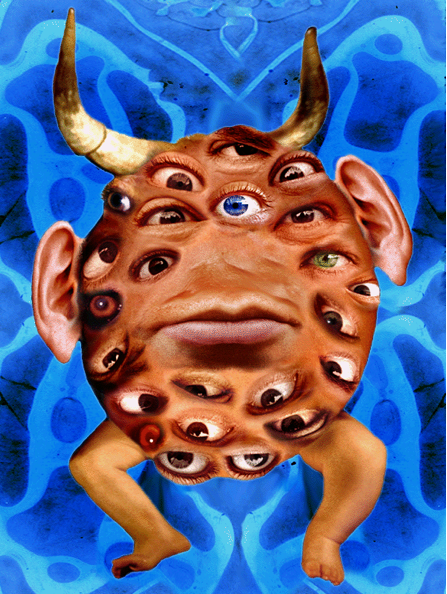
\includegraphics[width=6cm]{Fig1.png}
\caption{In EAX, one of \textit{Epizoo}'s screens, the eyes follow the mouse. The eyes,
mouth, ears and legs are hot spots that can be touched and clicked.}
\label{Jorda:fig:epizoo} 
\end{figure}

\subsection{Reintroducing FMOL (1997--2002)}

FMOL, a project I started in 1997  when the Catalan theatre group La Fura dels
Baus proposed to me the conception and development of an Internet-based music 
composition  system that could allow cyber-composers to participate in the
creation of the music for La Fura's next show, supersedes most of \textit{Epizoo}'s
musical limitations. The FMOL project has  evolved since  its  debut, and 
several articles  have  been  written  that should not be repeated here. The fact
is that FMOL exemplifies several paradigms which can be treated independently. It
is primarily a tool for collaborative  musical composition  on the Internet. This
feature that was the motto of the initial project is better  exposed  in  \cite{Jorda:1999}, 
which  deals  with  the  social  and aesthetic implications of net-music, and
 \cite{Jorda:2001} which cover more technical aspects of the implementation. Furthermore,
implications of computer and web based collective or collaborative  music 
composition  and  performance,  starting with the \textit{League of Automatic Composers} in  the  late  70s  \cite{Bischoff:1978} have been widely studied and published  in these last
years in papers and thesis such as \cite{Barbosa:2002} and \cite{Follmer:2001}.

Technical aspects of the FMOL software (real-time synthesis engine, etc.) are
covered in \cite{Jorda:1998}. The didactical, intuitive and proselytizing aspects of FMOL as a
tool for introducing newcomers into experimental electronic music are deeply
treated in \cite{Jorda:2002}, while \cite{Jorda:2002a} or \cite{Jorda:2002b} also cover its use as a professional  
instrument   and   its    attempt    at    dealing simultaneously   with  
micro-sonic and    macro-musical compositional ideas.

In this paper I want to focus only on the peculiar aspects brought by FMOL's
unique user interface, which presents a closed feedback loop between the sound
and the graphics: in FMOL, the same GUI works both as the input for sound  control and as an output that intuitively displays  all  the  sound  and music activity. After explaining
deeper this idea, I will discuss different ways where these sonic-graphic
relations are present in recent audiovisual software, and the path that has led
us to the conception of our new project, the reacTable*.

\subsection{FMOL Musical Output}

With FMOL I wanted to introduce newcomers to experimental electronic music
making. Therefore, for obvious availability reasons,  the instrument  had to be a
mouse-driven software (it can still be  freely  downloaded  at  \cite{Jorda:2002}).  I  also
wanted to create a simple and complex tool  all at once; a tool that would not
dishearten hobbyist musicians, but would still be able to produce completely
diverse music, allowing a rich and intricate control  and  offering  various 
stages of training and different learning curves.

Both goals have been, in my opinion, quite well attained. During the two
Internet calls for musical contributions  for two of La Fura's shows
(January-April 1998 for F@ust 3.0, and September-October 2000  for the opera DQ)
more than  1,700 compositions were received in the database. We know now
that many of the participants had no prior contact with experimental electronic
music and that a few were even composing or playing for the first time, but the
final quality of the contributions (which can be heard online, as well as on the
the Furadels Baus' F@ust 3.0-FMOLCD published in 1998 \cite{Jorda:1999}, and on the more
recent CMJ 2002 companion CD \cite{CMJ:2002}) was quite impressive.

Moreover, I have given several  FMOL workshops  usually with a mix of
musicians and non-musicians,  and if the feeling is positive they usually end
with public concerts. An improvisation fragment recorded after one of these
workshops can also be heard in the CMJ CD \cite{CMJ:2002}. The intuitiveness acid test took place in
March 2003 during a one-day workshop with 5 to 8-year old kids from Galicia
(Spain), which ended with surprising collective  improvisations.

It takes about half-hour to start having fun with the instrument, and several
hours  to acquire some confidence and produce controllable results. However,
after five years of playing it, I am still  learning it and do often discover
hidden features.  Because,  and  that  is  another  important  point,  it
happens that the instrument I originally designed as  a cheap and freely
available system for ``experimental electronic music proselytism,'' turned to be,
to my own surprise, my favorite instrument for live concerts. Since 1999, the
FMOL Trio (Cristina Casanova and me on FMOL computers, plus Pelayo F.
Arrizabalaga on saxophones/bass clarinet and turntables) performs free-form
improvised electronic music and has produced several live CDs \cite{Feller:2002,Trio:2000,Trio:2002,Trio:2002a}.

\subsection{FMOL Visual Feedback}

Arguably, visual feedback is not very important  for playing traditional 
instruments,  as   the   list   of   first   rank   blind musicians and
instrumentalists (e.g. Ray Charles, Roland Kirk, Tete Montoliu, Joaqu\'{\i}n
Rodrigo, Stevie Wonder \ldots{}) may suggest. But traditional instruments usually
bring  other kinds of feedback, like haptic  feedback \cite{Bongers:1994,Gillespie:1999}, which is 
not  so often  present  in  digital  instruments, at  least  in  the  ``cheap''
ones. Besides, why should not digital  instruments  use at their advantage
anything that could broaden the communication channel with its player? I am
convinced that in the case of FMOL, its unique visual feedback has been a
fundamental component for its success as a powerful and at the same time
intuitive and enjoyable instrument.

FMOL mouse-controlled GUI is so tightly related to the synthesis engine 
architecture, that almost every feature of the synthesizer is reflected in a symbolic, dynamic and non-technical way in the interface. In  its  rest position  the  screen looks like a simple 6x6 grid or lattice. Each of the six vertical lines is associated with  one  voice  generator (FMOL's sound engine supports six real-time synthesized stereo audio tracks or channels), while the horizontal lines are associated  with the effects processors
(filters, reverbs, delays, resonators, frequency, amplitude  or ring  modulators,
 etc.), embedded  in each track. All of these lines work both as input devices
(controllers) that can be picked and dragged with  the  mouse, and as output
devices that give dynamic visual and ``sonic'' feedback.

\begin{figure}[t]
\centering
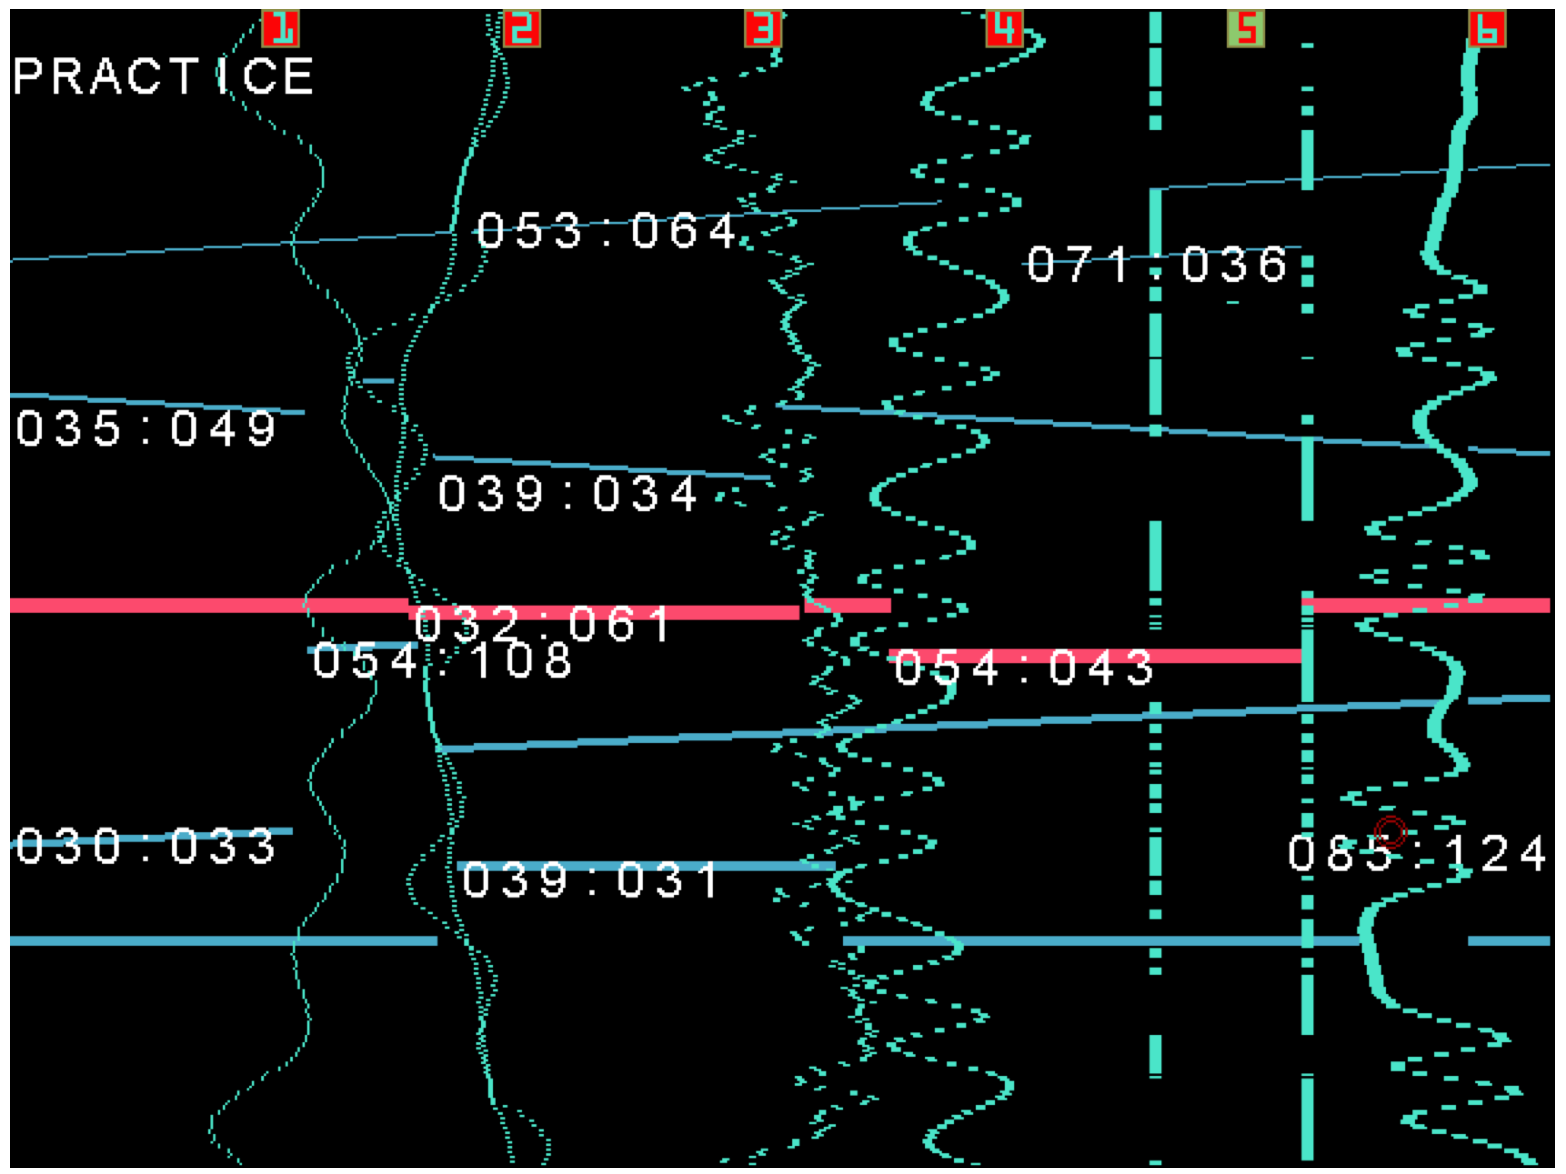
\includegraphics[width=9cm]{jorda-fig2.png}
\caption{FMOL in action.}
\label{Jorda:fig:fmol} 
\end{figure}

Mappings and detailed control mechanisms are explained better in \cite{Jorda:2002}. The key
point  is that when multiple  oscillators or segments are active (FMOL engine
includes 24 LFOs and 96 parameters to control), the resulting geometric
``dance,'' combined  with  the   six-channel  oscilloscope information given by
the strings, tightly reflects the temporal activity  and intensity of the piece
and gives multidimensional  cues to the player. Looking at a screen like Figure~\ref{Jorda:fig:fmol}
(which is taken from a quite dense FMOL fragment), the player can intuitively
feel the loudness, frequency  and  timbrical  content  of every channel, the
amount of different applied effects, and the activity of each of the 24 LFOs.
Besides, no indirection is  needed  to  modify any of these parameters, as
anything in the screen behaves simultaneously as an output and as an input.

\section{Sonigraphical Tools}

\subsection{Media players and VJ Tools}

In order to show the secular catacomb stage of visual  music, Bernard Klein
affirmed in his 1927 book  \textit{Color-Music:  the Art of Light} that ``it is an odd
fact that almost everyone who develops a color-organ is under the misapprehension
that  he or she, is the first mortal to attempt to do so'' \cite{Klein:1927}. This assessment
could surely not be pronounced anymore nowadays.  While  since  its  beginning, 
digital  technologies have boosted multimodality and any kind of parallelism
between image and sound in any of  their  two directions,  the truth is that in
the last few years, we have seen the flourishing of many software programs or
environments that deal with this duality in several ways, even creating
distinct families of tools each with its well defined idiosyncrasy.

Following the trend started with the popular music visualization freeware
program \textit{Cthugha} released around 1994 and described  on  its  birth  as \textit{an 
oscilloscope  on  acid}, current software  music  players,  like  \textit{WinAmp} or 
\textit{MS Media Player}, come with dozens of fancy visualization  plug-ins,  that allow  the  user  to  view  the  results  of  the  music  in  many different ways. These
systems can be generally described with the following scheme.

\begin{figure}[t]
\centering
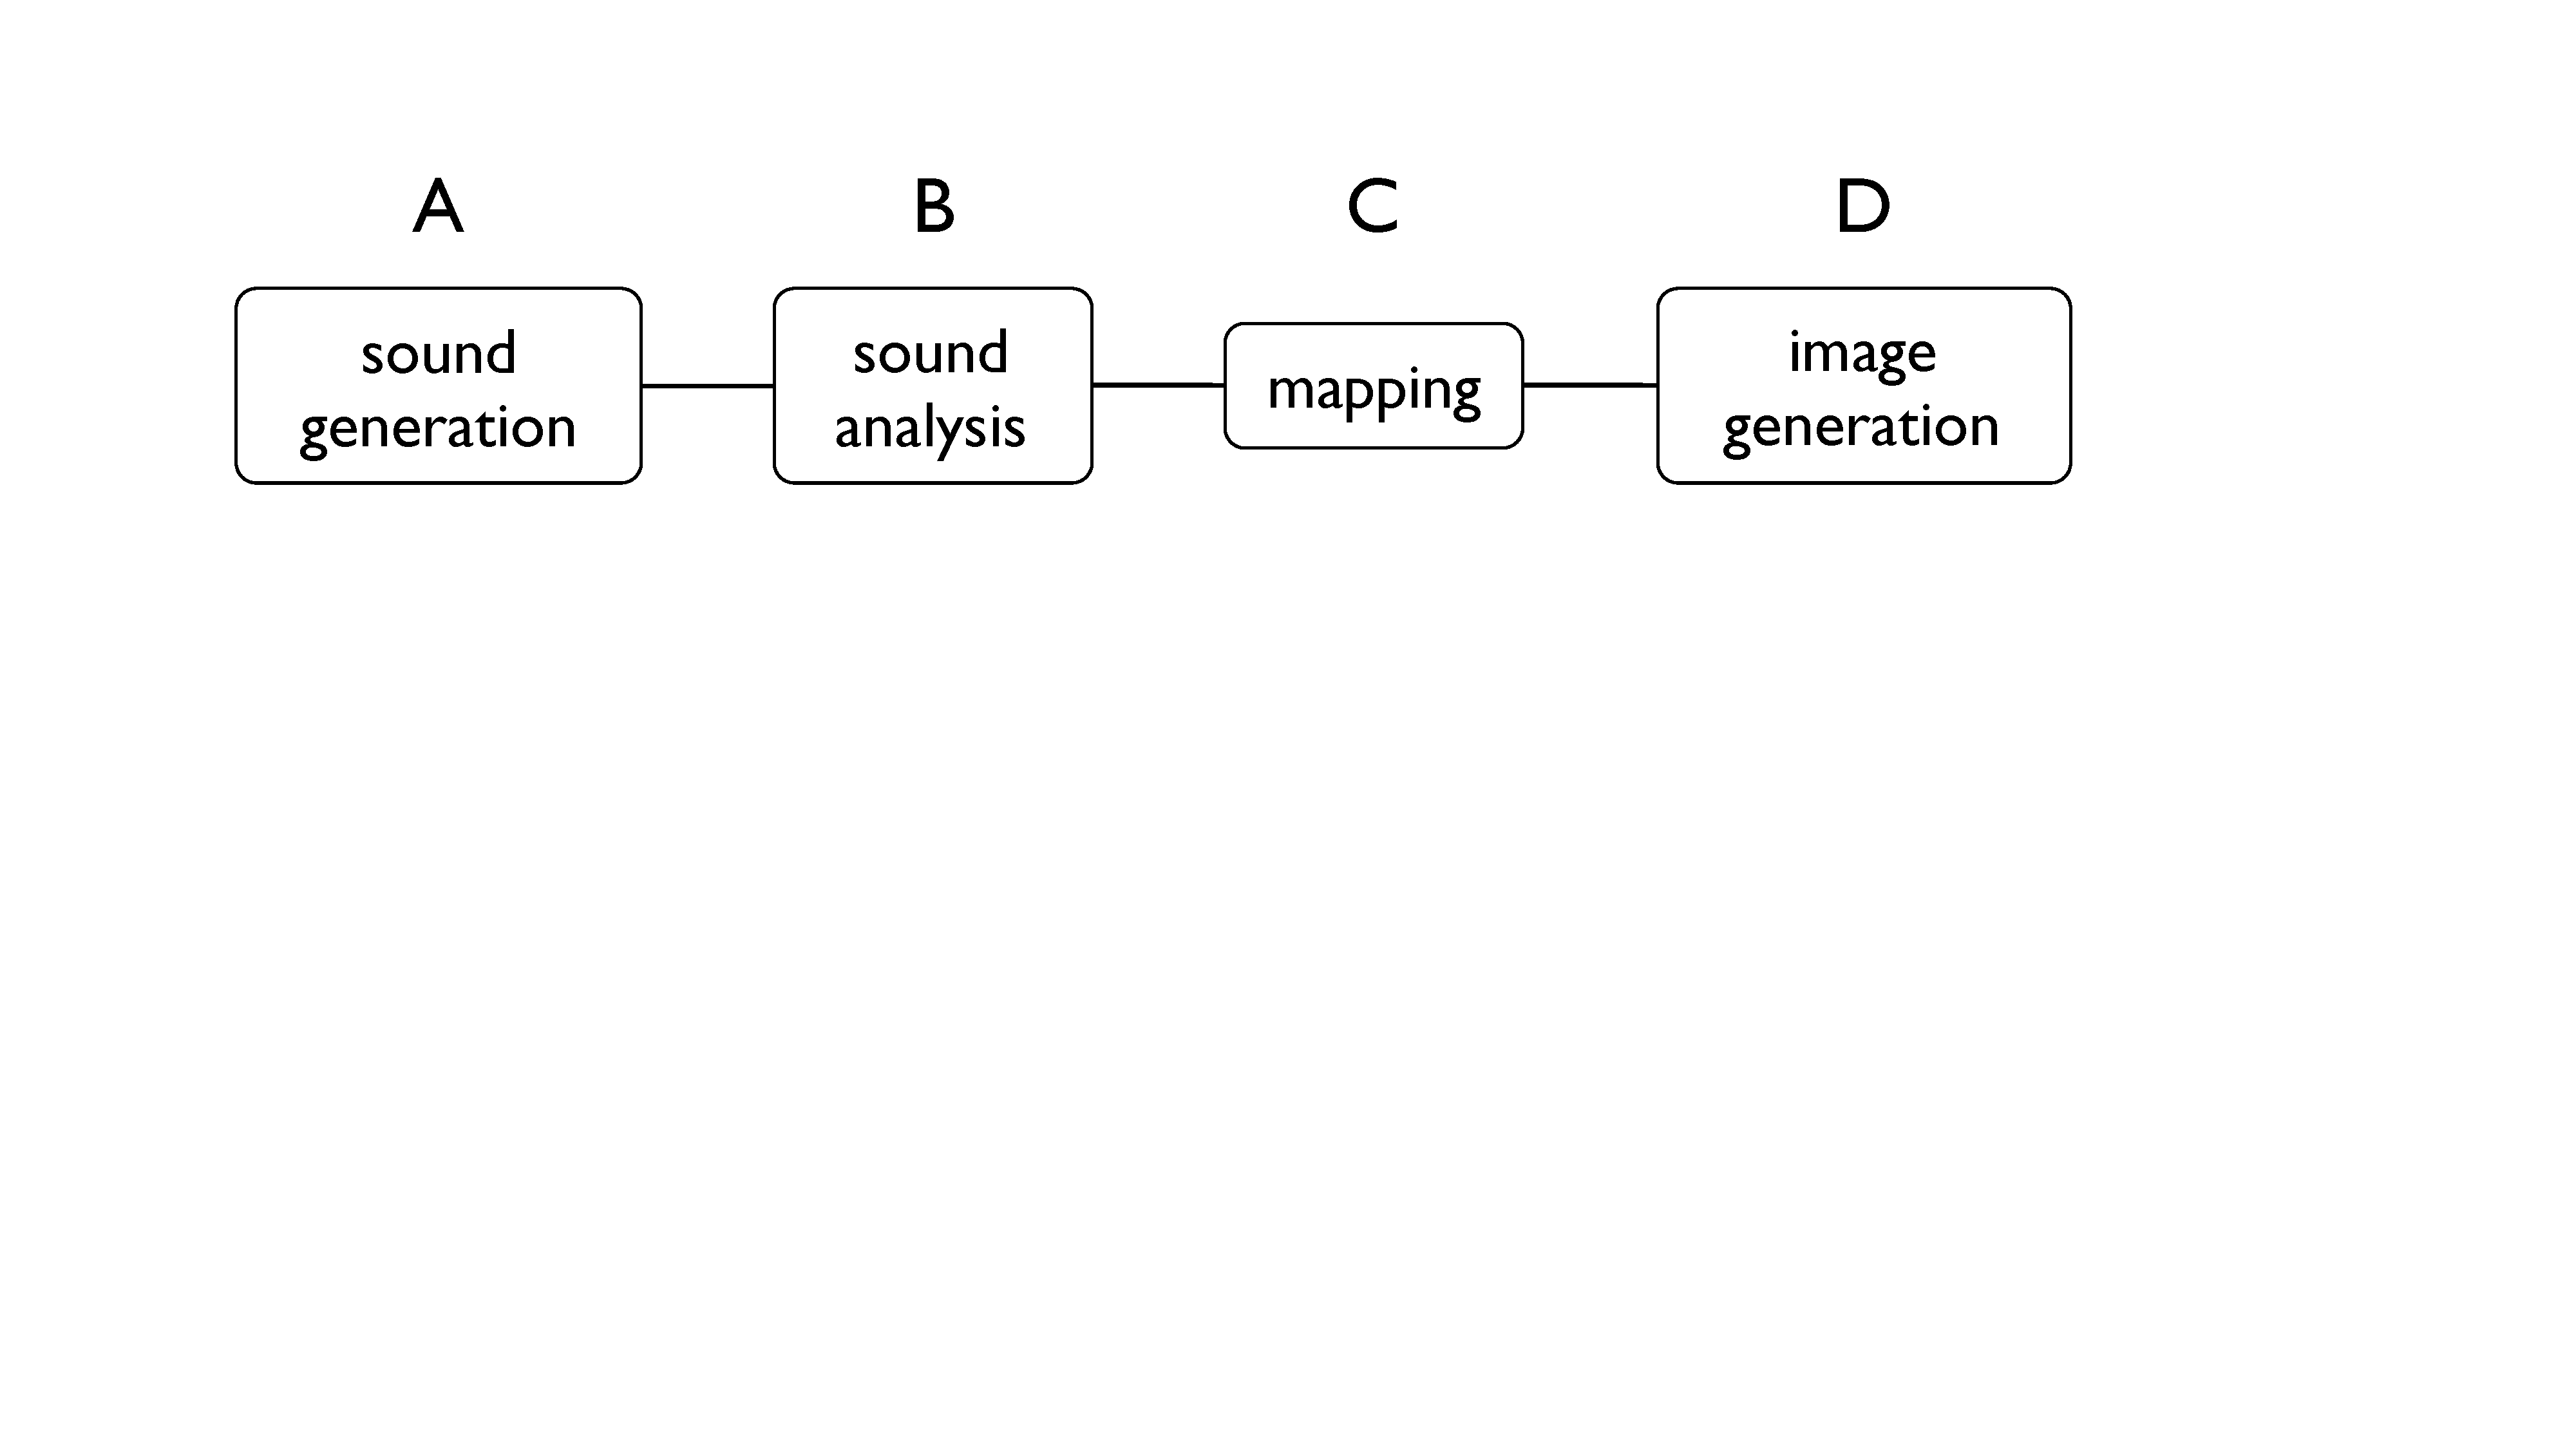
\includegraphics[width=9cm]{jorda-fig3.pdf}
\caption{Elements of a standard music player with visualization.}
\label{Jorda:fig:music-player} 
\end{figure}

However, these systems are not very interactive, except that users can decide to change the visualization  plug-in,  applying thus a discrete change to block D. When an audio-visualizer  of this kind becomes interactive, we have what we could call a VJ Tool. Such tools exist as stand-alone programs such as Jaromil's \textit{FreeJ}, \textit{Arkaos} or \textit{Resolume}, or can be easily  built using  visual  programming  environments  like MAX + (Nato or Jitter), or PD + (GEM or Framestein), to name a few of the more popular software combinations.

In this new case, depending on the particular system design, the user could
interact at any step of the chain.

Using the aforementioned programming environments, one can also decide to take
the complementary approach, and build a musical instrument or a sound
synthesizer which can be directly controlled by the analysis of some dynamic
visuals. These image input can be of  any  kind  (synthetic,  abstract, video,
etc.), and can come from any source (stored movies, real-time generated
animations, live video input, etc.) Although different in concept, this
alternative scheme could also include computer vision based musical controllers.

\begin{figure}[t]
\centering
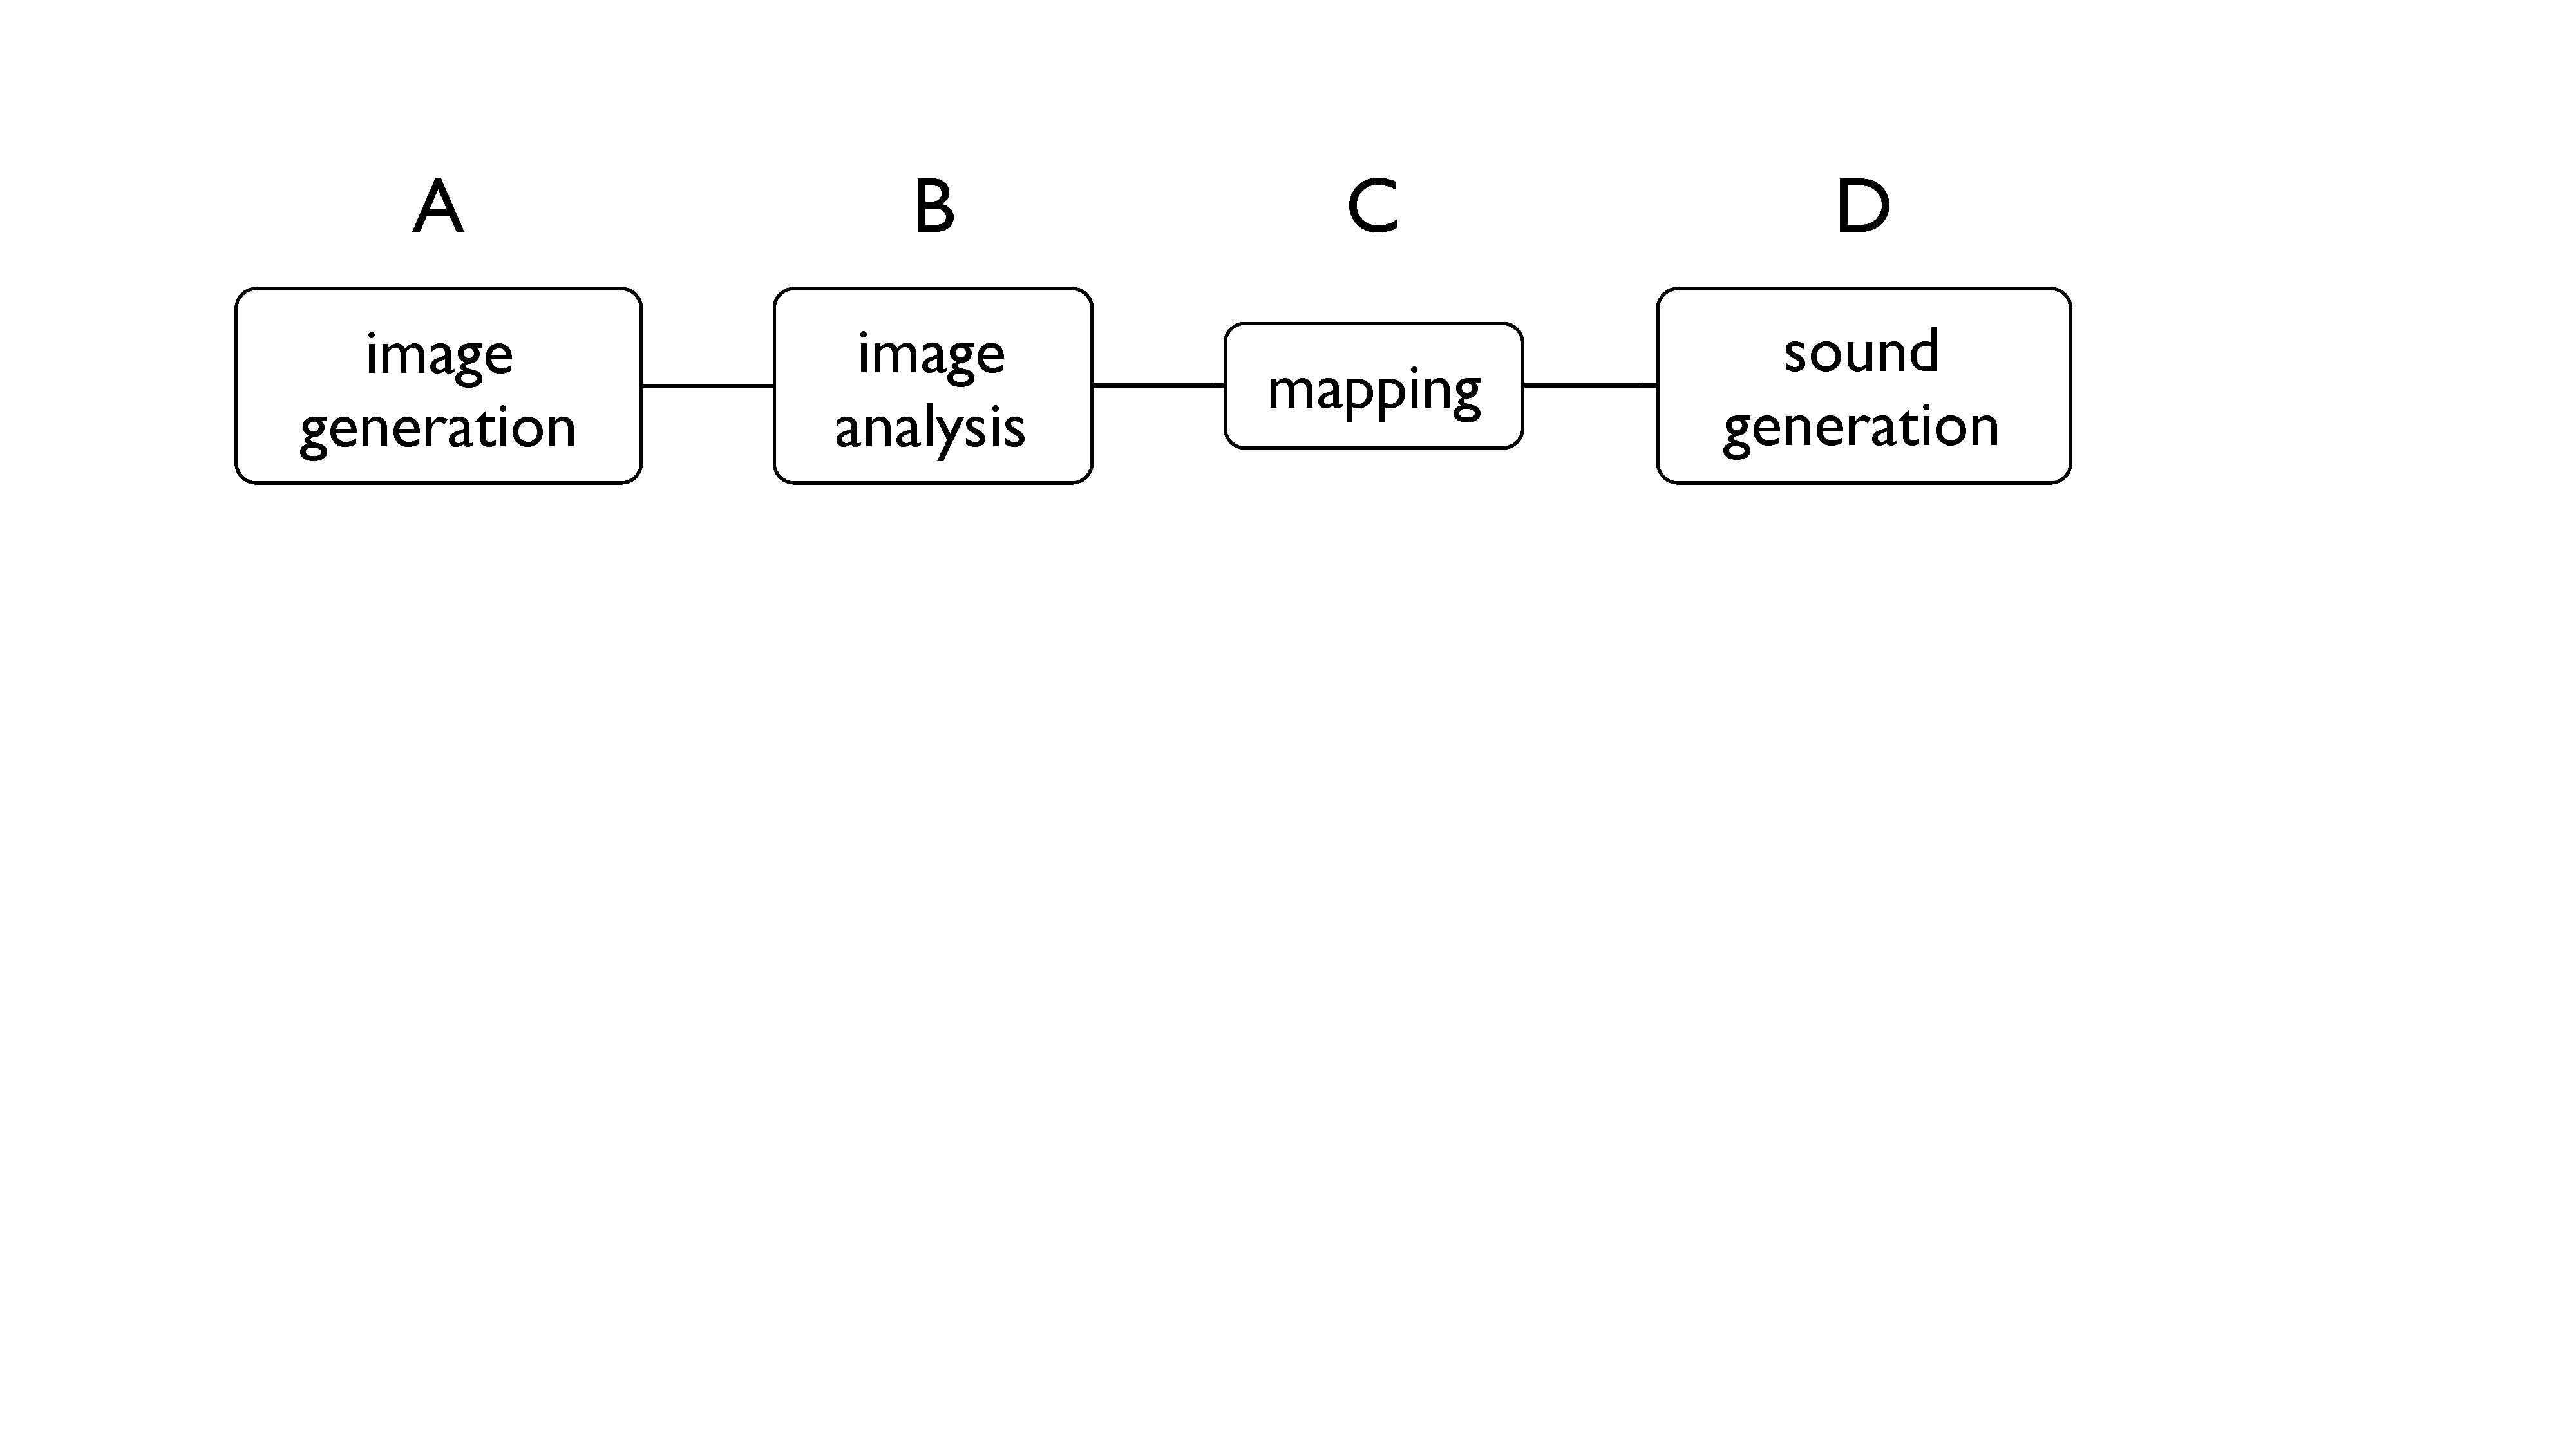
\includegraphics[width=9cm]{jorda-fig4.pdf}
\caption{Elements of an image controlled  music generator.}
\label{Jorda:fig:generator} 
\end{figure}

However, neither of these two approaches (Sound $\rightarrow$ Visuals  or Visuals
$\rightarrow$ Sound)  generally  closes  the  control  loop  as FMOL does
(i.e. in VJ tools, the way the user modifies the graphics does not affect the
music). Besides, they usually present two  windows  at least:  one  for the 
visual  output  (or input, depending on the chosen approach)  and  an additional
one (the ``control panel'') for parameter modification; they do not allow to
modify the \textit{visuals window} by playing directly on it.

\subsection{Golan Levin's Work}

To my knowledge, only Golan Levin's work follows an audiovisual approach
comparable to the one I've presented in FMOL. The fact is that  although  we
unfortunately  did not know about each other until quite recently, I believe
our goals and approaches share many common aspects.  In  his  master thesis
``Painterly Interfaces for Audiovisual Performance'' he proposes a system for the
creation and performance of dynamic imagery and sound, simultaneously, in
real-time, and with basic principles of operation easy to deduce, while at the
same time capable of sophisticated expressions and indefinitely master-able \cite{Levin:2000}.

\begin{figure}[t]
\centering
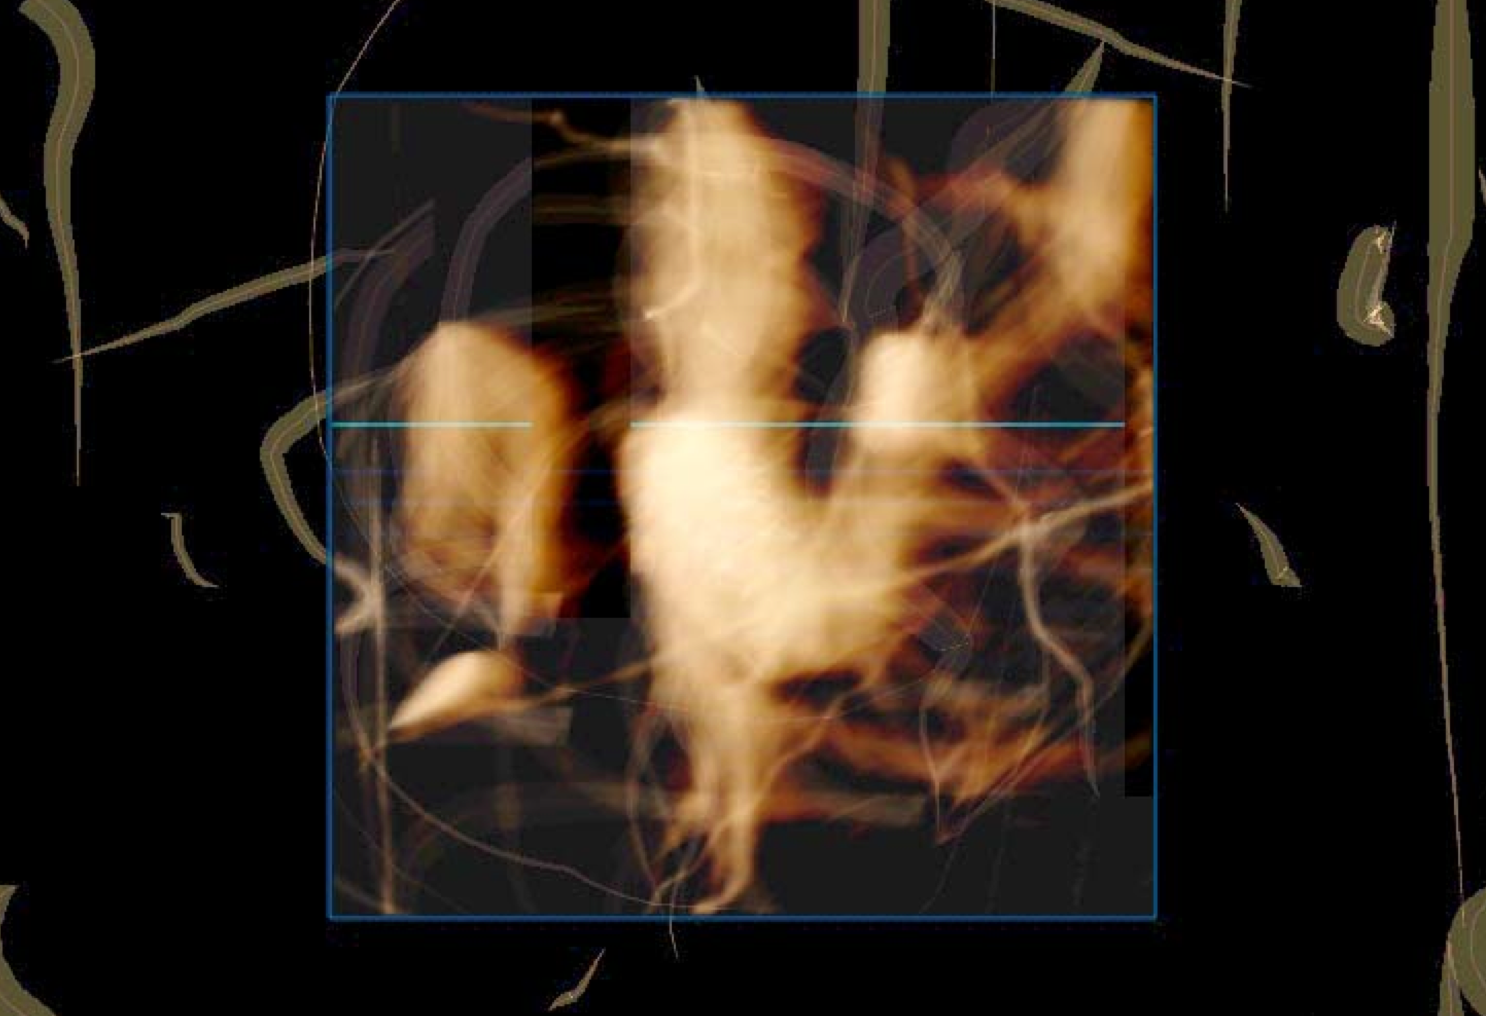
\includegraphics[width=9cm]{jorda-fig5.png}
\caption{A screenshot  of Golan Levin's Yellowtail.}
\label{Jorda:fig:yellowtail} 
\end{figure}

Levin talks about an inexhaustible, extremely variable, dynamic, audiovisual
substance that can be freely painted, and he  has  developed  many  audiovisual  
tools,  like  \textit{Yellotail}, \textit{Loom}, \textit{Warbo}, \textit{Aurora},  and  \textit{Floo}, which  follow  this  path. Perhaps, the major difference in our approaches may be the fact that Levin, like Oskar Fischinger, the animator that in the 40s invented the \textit{Lumigraph} color organ \cite{Moritz:1997}, is willing to play light while playing sound.  For him, image is therefore an end in itself. While for me, it is only  the means to an end: a
more intuitive interface for creating music.

\section{The reacTable*}

\subsection{Preliminary}

Last year, together with the doctorate students  Alvaro Barbosa,    Gunter   
Geiger,    Rub\'{e}n    Hinojosa,    Martin Kaltenbrunner and Jos\'{e} Lozano,
and the  undergraduate students Carlos Manias and Xavier Rubio, we constituted
the Interactive Systems Team, inside the Music Technology Group led by Xavier
Serra at the Pompeu Fabra University of Barcelona. One of the initial projects
was to port FMOL  to Linux and make it open-source, which seemed also a good
opportunity for revamping the system.

Looking at the way people have used  FMOL, and  using  it myself for
improvisation in different contexts and with different musicians, has raised
ideas new features and modifications. But we also felt that  this  control 
complexity could not be permanently increased; there  are limits  to  what can be
efficiently achieved in real-time by means of  a mouse and a computer keyboard.
Building an external FMOL controller for a faster and more precise
multi-parametric control seemed therefore a tempting idea. Designing  a video
detection or ultrasound system that would  allow musicians  to  interact on a big
projection  screen, grabbing  and moving  strings  with their hands, was the
first idea we had. This could surely add a lot of visual impact to live concerts,
although we also felt that musical control and performance may not necessarily
improve with it. These and other considerations took us to a completely new path,
which should profit  the  knowledge  gained  during this years and bring it to a
much more ambitious  project: The reacTable*.

\subsection{Intentions}

We aim at the creation of a state-of-the-art interactive music instrument, which
should be collaborative (off and on-line), intuitive   ( zero manual,   zero instructions),   sonically challenging and interesting, learnable, suitable for
complete novices (in installations), suitable for advanced electronic musicians
(in concerts) and  totally  controllable  (no  random, no hidden presets\ldots{}). The reacTable*  should  use  no  mouse, no keyboard,  no  cables,  no  wearables.  It  should   allow  a flexible number of users, and these should  be able to enter or leave the  instrument installation   without previous announcements. The technology involved should be, in one word, completely transparent.

\subsection{Computer Vision and Tangible  Objects}

As the Tangible Media Group directed by Professor Hiroshi Ishii at the
MIT Media Lab states, ``People have developed sophisticated skills for sensing 
and  manipulating our physical environments. However, most of these skills are  not employed by traditional GUI\ldots{}. The goal is to change the \textit{painted bits}
of GUIs to \textit{tangible  bits}, taking  advantage of the richness of multimodal human
senses and skills developed through our lifetime of interaction with the physical
world.'' \cite{Ishii:1997}.  Several  tangible  systems  have  been  constructed based on
this philosophy. Some for musical applications,  like \textit{SmallFish}, the 
\textit{Jam-O-Drum} \cite{Blaine:2000,Blaine:2002}, the  \textit{Musical Trinkets} \cite{Paradiso:2000a}, \textit{Augmented Groove} \cite{Poupyrev:2000} or the \textit{Audiopad} \cite{Patten:2002}, but we believe that no one attempts the level of integration, power and flexibility we propose.

\begin{equation*}
\texttt{reacTable* = FMOL + MAX + Jam-O-Drum}
\end{equation*}

Substitute if  you  want  \textit{MAX} with \textit{PD} or \textit{JMax} or  even \textit{AudioMulch}. Substitute the \textit{Jam-O-Drum} with the table version of \textit{Small Fish}. You can even substitute FMOL, but only  with Levin's systems, and you will get an initial idea about what the reacTable* is all about:  a table-based collaborative  music instrument that uses computer vision and  tangible user interfaces technologies, within a MAX-like architecture  and scheduler, and with FMOL-inspired HCI models and visual feedback.

The reacTable* is a musical instrument based  on  a round table,  which  has  no
 sensors,  no  cables,  no   graphics  or drawings. A video camera permanently
analyses the surface of the table, while a projector draws a dynamic and
interactive interface on it.

Many interesting and promising computer vision tools, mostly based on body
motion capture, are being developed  for musical applications \cite{Camurri:2001,Camurri:2002}. 
However, many of us  do  not feel too comfortable ``dancing'' in front of a
video camera (some even without camera!), while we all work and socialize around
tables. For this reason our computer vision  system  does  not attempt to track
body motion. Instead, it focuses on  tracking the  hand  movements  over  the 
table,  and  on  detecting  the nature, position and orientation of the objects
that are distributed on its surface.

These objects are mostly passive and made out of plastic  or wood of different
shapes. Users interact with them by moving them,  changing  their  orientation 
on   the   table   plane   or changing their faces (in the case of volumetric
objects). More complex  objects  include  (but  are  not  limited  to)  flexible
plastic tubes for continuous multi-parametric control, little wooden dummy
1-octave keyboards, combs (for comb-filters), or other everyday objects. In case
an object needs sensors, its communication with the host computer will be
wireless.

\subsection{Visuals (1)}

The projection  follows  the  objects  on  the  table  wrapping them with auras
or drawing figures on top of them. The projection covers also the  whole table 
surface with dynamic and abstract elements that reflect all the system's
activity, and depend on the hands' movements and trajectories, the objects' types
and positions, and the relations  between them all. The projection never shows buttons or widgets of any kind.

\begin{figure}[t]
\centering
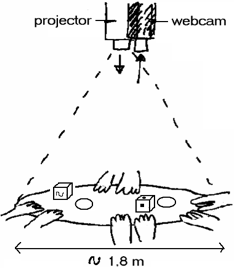
\includegraphics[width=60mm]{Fig6.png}
\caption{The reacTable* simplified scheme.}
\label{Jorda:fig:reactable-simplified} 
\end{figure}


\subsection{But where is MAX?}

FMOL has proven to be quite flexible. Its palette of sound generators and
processors includes  more than  20  algorithms that (with internal configuration 
variations)  constitute a bank of  127  presets the  user  can  select and 
apply to  any  of  the strings. This process of ``building an orchestra'' is not
done in real-time while playing, but in a different, more conventional window.
Besides, all FMOL macro-control of form is done like in traditional analog
synthesizers, by means of LFOs and arpeggiators. More sophisticated control
sources, such as algorithmic generators, pitch filters, etc. cannot fit
coherently into the FMOL interface. The reacTable* overcomes these restrictions
by adapting one of the more powerful real-time computer music software paradigms
implemented in the last decades.

Like  MAX  and  all  of  its  cousins,  the  reacTable* distinguishes between
control and sound objects, and between control and sound  connections.  Unlike 
MAX, and  more like Audiomulch (which however has no explicit  control flux), the
reacTable*  objects are more high-leveled; the  reacTable*  is an ambitious
project but  it  \underline{is} an  instrument, not  a programming language!

When a control flow is established between two objects, a thick straight line is
drawn between them, showing by means of  dynamic animations, the  flux 
direction,  its  rate  and  its intensity. Visual feedback will also guarantee
that LFOs and other  macro-temporal  values  will  be  perceived  as  blinking animations projected on top of the related objects, showing frequency and
shape (e.g. square vs. sinusoidal).

\subsection{Visuals (2): Audio flow}

Where control flow lines are straight and simple, audio flow lines are \textit{organic}
and  complex.  Their  dynamic  shapes  will show the macrotemporal audio
variations (vibratos, tremolos, tempo and rhythms\ldots{}) and their interior
(colors, intensities\ldots{}) will depend on their spectral audio content.

\begin{figure}[t]
\centering
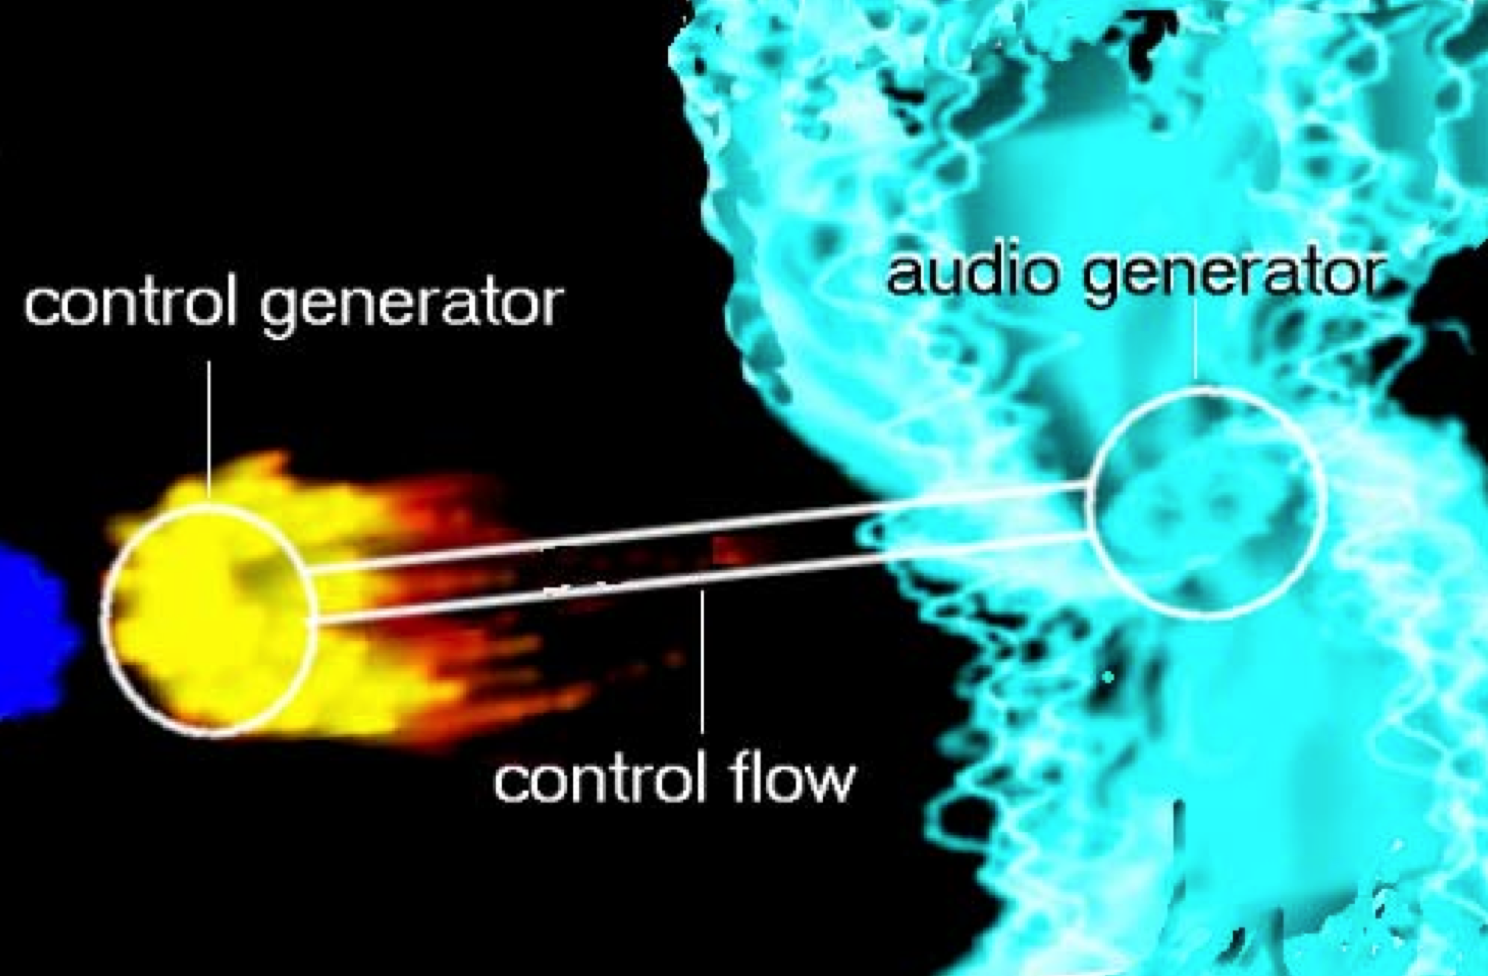
\includegraphics[width=9cm]{jorda-fig7.png}
\caption{Control  and audio flow simulation.}
\label{Jorda:fig:control-audio-flow} 
\end{figure}

Users  will also be able to control, modify or  fork  audio flows  without 
using  additional  objects,  but  just  by  waving their hands, as if they were
digging water channels in the beach sand.

\subsection{Avoid user's frustration at any cost}
To avoid frustrations, a system does not necessarily have to be completely
understandable, but it has to be coherent and responsible. Unlike MAX, the
reacTable* has to work ``by default'' and any gesture has to produce audible
results.  Here are some of its laws:

\begin{itemize}
\item There is not anything like an \textit{editing  mode}
and  \textit{running mode} (at least for \textit{installation  users}); the  reacTable*  is always running and always being edited!
\item Objects are not active until they are touched
\item Active objects have a dynamic visual \textit{aura}
\item Objects are interconnected by proximity
\item If, on  start-up, a  user  activates an  object that  does not sound (e.g. a control  object)  the  closest  audio object is automatically linked to it, and the link is visualized
\item Moving an object on the  table  can change the  relations with the other objects
\item Relations can also be ``fixed'' touching two objects  with the two hands. Fixed links are shown with a thicker line or a different color
\end{itemize}

Perry Cook, in an informal music controllers design decalogue, ironically points
that ``smart instruments are often not smart.'' \cite{Cook:2001}. Although  we
basically  agree with  him, we have come to the conclusion that a system like the
reacTable* must show some kind of intelligent  behavior. For example, as most of
the control objects are adimensional (some, like the dummy keyboard, are not),
when  one  adimensional  control flux is sent to an object that can accept
different inputs, the system chooses what the best parameters to  control  in 
every case are. In another demonstration  of intelligent  behavior, the system
may suggest interesting candidates for a given configuration, by highlighting 
the appropriate objects (in a manner not to be confused with LFOs).

The reacTable*  wants to be  \textit{user-proof}. For  instance,  it seems  natural 
that  after  some  minutes,  people  will  start stressing the system in
different ways, like placing personal objects onto the table. Although it is not
possible  to anticipate all objects  that  people  may use, some of the  more
common could be detected (cigarette packets, mobile phones, keys, pens\ldots{})
and a ``funny'' functionality could be  added  to  them (e.g. mobiles could
generate pitch in a ``mobile-fashion'').

\section  {Current Implementation}

The reacTable* project has started in December 2002 coinciding  with  the 
foundation  of  the  Interactivity  Team within the Music Technology Group (MTG).
We are currently working and researching all the main threads in parallel
(computer vision and objects recognition, sound engine architecture, 
interactivity  logic,  sound  visualization,  etc.) while designing the core and
the integration of all these branches. Computer vision and object recognition is
being carried using both \textit{Eyesweb} \cite{Camurri:1999,Camurri:2000} and the Intel Image Processing (IPL) and Open Computer Vision (OpenCV) libraries.\footnote{\url{http://opencv.org/}} We will
not describe here any of these issues, as we soon plan to devote a whole paper to
them. The synthesis engine is  being  implemented  using  the  CLAM libraries, 
the open-source, multi-platform C++ libraries for real-time audio being developed
at the MTG \cite{Amatriain:2002,Amatriain:2002a}.

In parallel with these two main productions  threads, we are working with a
reacTable* software-only simulator  (that runs on both Linux and Windows), which
is an essential  workbench for defining  and  refining  all  of the  system 
laws, evaluating user interaction and objects' connectivity rules, as well as
determining  the  panoply  of  sound  and  music  objects,  their roles,
behaviors, the way they synchronize between them, etc. The simulator GUI has been
 implemented  in  Java by  Martin Kaltenbrunner, while Gunter Geiger is  working 
on  its  sound engine using PD for quick prototyping. Both modules communicate
via TCP/IP, a flexible architecture which also permits multi-user simulation by 
running  different  instances of the GUI in different computers.

Figure~\ref{Jorda:fig:reactable-simulator} shows  a  reacTable*  simulator  screenshot,  with only four kinds of
sound  objects:  High Frequency Oscillators (circles), Low Frequency Oscillators
(triangles), filters (smoothed squares) and time-based effects (squares). Visual
feedback is yet very simple; all connection lines  are straight and do not
suggest therefore any of the information they transmit, except that to
distinguish between the two types of connections, audio lines are drawn in dark,
while control  lines are light grey. Each dark line  flowing  into  the  audio  sink represented by the black central circle corresponds therefore to an
independent audio thread.

\begin{figure}[t]
\centering
\includegraphics[width=8cm]{Fig8.png}
\caption{reacTable*  simulator snapshot.}
\label{Jorda:fig:reactable-simulator} 
\end{figure}

At this early stage, what we have is  a sort  of higher  level MAX in which
users can drag objects that dynamically interconnect between them according to 
the  rules  defined  in the system. Using the right mouse button objects can
also spin around and connection lines can be broken. Parameters are calculated
from the  rotation angle of  the  objects as  well  as from the length and the orientation of their connections. As simple as it still is, this flexible and dynamic architecture already permits for some fast sound changes that seem impossible to attain in an analog modular synthesizer, which it somehow evokes.

\section {Future Work and Conclusion}

The reacTable*  is an ambitious project. Unlike  many new designed instruments,
its origin does not come from approaching its creation by exploring the
possibilities of a specific technology, nor from the perspective of mimicking a
known instrumental model. The reacTable* comes from our experience designing 
instruments,  making  music  with  them, and listening and watching the way
others have played them. Needless to say, we have deposited a great hope and
expectation on  it.  We  plan  to  have  the  first  integrated  by autumn 2003
and a first full working version by spring 2004.

\begin{acknowledgement}
I would like to thank all the members of the Interactive Systems Team, and
specially  Martin  Kaltenbrunner, for their suggestions on this paper, and Xavier
Serra for his support on this project.
\end{acknowledgement}

\section*{Author commentary: The Genesis of Reactable}
\paragraph{Sergi Jord\`{a}}

2003, the year of the 3\textsuperscript{rd} NIME conference, was also quite an impasse year for me. After graduating in physics in the mid-80s and spending most of the 90s working as a freelance interactive and media artist/designer/programmer, developing interactive installations, performances and music systems (two of them, \textit{Epizoo} and FMOL, had already been introduced in my 2001 NIME paper). With the advent of the millennium I had decided to re-enter academia and pursue a PhD in Computer Music at the Music Technology Group (MTG) founded by Xavier Serra in Barcelona. The MTG was still a very young research group in which the lack of professors or post-docs (Serra was still the only doctor!) was happily compensated with the enthusiasm of everyone, and the most mature PhD candidates shouldered the role of team and project leaders. So here I was, trying to figure out my own PhD thesis, while simultaneously coordinating a team of PhD students that included some of the most talented computer music developers I have ever known. It is within these circumstances that this paper provides an analytical revision of some of my past works and discusses  prospective research directions.

Through the study of the aforementioned examples (\textit{Epizoo} and FMOL), the first half of the paper addresses the potential of what I then called ``sonigraphical instruments,'' a term I coined for referring to instruments in which their GUI acts both as an input for sound control, and as an output that provides a summarized and quickly graspable display of all the sound and music activity. This sonigraphical feature, I argued, is even more pertinent in multithreaded instruments that allow several simultaneous musical processes. These postulates would be furthered in my Phd dissertation published two years later \cite{Jorda:2005}. 

The second half of the paper introduces a multithreaded and sonigraphical DMI, Reactable (known as reacTable* at that time), discussing its main features and the  rationale behind its conception. Considering that this part describes a system that had not yet been tested, not implemented, and in fact, not even fully technically solved, that is, that what it outlines is little more than a personal vision, I now wonder how unlikely it would be that a similar paper would have been accepted in 2015! The presumable different perspectives resultant from this dozen year gap, reflect on one side the maturity currently attained by the NIME field, which was in its infancy in 2003. They could also warn us however about the risks of trying to address too scientifically topics such as the design and evaluation of DMIs, which resist reduction and systematization. For example, although we have published several papers that systemically study the potential benefits of the Reactable in very specific contexts, such as autism \cite{Xambo:2013} or collaboration and peer-learning in public spaces, we have still failed to produce the ``ultimate Reactable-music-instrument evaluation'' paper.

A few months after the publication of this paper, we solved the most crucial pending technical issue and published reacTIVision, an open-source, cross-platform computer vision framework for the tracking of fiducial markers and combined multi-touch finger tracking \cite{Bencina:2005}. Two years later, Reactable was premiered at the ICMC 2005 in Barcelona. It had not been the first musical tabletop; at least the Audiopad \cite{Patten:2002} and the Music Table anticipated it, but it became the more popular one and, arguably,  the most popular DMI to emerge from an academic context. In November 2006 we guilelessly published a video in YouTube, which rapidly and unexpectedly reached millions of views. Three months later, Bj\"{o}rk contacted us and in April 2007 she started touring with a Reactable. Around this same period, the Reactable team also started touring extensively, giving more than 300 concerts, installations and presentations, in 25 countries during the next 3 years. This helped enormously with fine-tuning and improving the system. In 2008 I published what I consider the ``ultimate'' Reactable paper \cite{Jorda:2008}. In 2009, the company Reactable Systems\footnote{\url{http://reactable.com/}} was founded, launching the Reactable Live and the Reactable Experience, and later in 2010, also Reactable Mobile for iOS and Android. 

With Reactable Systems monopolising all the development of the musical instrument, my research shifted towards other areas of tabletop and tangible interaction. It has just recently shifted back to NIME and digital music creation in the shape of ``expert agents for electronic music performance,'' combining research and techniques from musicology, music information research (MIR), machine learning and HCI.\footnote{\url{http://www.giantsteps-project.eu/}} My life has not changed so much, but this 2003 paper set the beginning of a nice story that has not yet ended, and I am definitely happy and proud with what we achieved.

\section*{Expert commentary: Pursuing a Sonigraphical Ideal at the Dawn of the NIME Epoch}
\paragraph{Charles Martin}

A common criticism levelled at the NIME community is that we jump onto the latest available technology, develop one interface, play one concert, send out a paper, and move on. To this criticism, Jord\`{a}'s work on sonigraphical instruments sits as a compelling counter-example.
Jord\`{a}'s paper seems to have appeared at a turning point in his work developing computer-based instruments for collaborative musical interaction, and to be representative of the start of the NIME epoch.

In the first half of his article, Jord\`{a} describes \textit{Epizoo}, a game-like multimedia interface that sits very much in the early-1990s, and FMOL, a collaborative synthesiser running in a late-90s era mouse-driven Windows interface. In the second half, Jord\`{a} outlines the in-progress design for Reactable, a table-top tangible interface that went on to be unveiled through YouTube videos\footnote{\url{https://youtu.be/0h-RhyopUmc}} in 2006 to mainstream acclaim in the tech and music press, and was famously used in Bj\"{o}rk's Volta \cite{Andrews:2007} and Biophilia concert tours starting in 2007. The Reactable could be said to be emblematic of a surge of interest in NIME-research around this time---at least that's when I started to get interested!

So what lessons does this paper hold for the NIME researcher of today?
First of all, this paper shows how perspective and experience acquired through long-term effort in developing musical interfaces is often required for the most interesting designs. The paper itself describes around 10 years of work where Jord\`{a} and his collaborators produced interfaces and invited beginners as well as experienced performers to use them. While Jord\`{a} is satisfied with the utility of FMOL, a successful design by all accounts, years of experience have suggested that there is potential to develop an instrument that is even more intuitive, collaborative, and with fewer compositional assumptions. More than 10 years later, we now know that Reactable achieved these goals, with success as an installation work, as an instrument on the professional concert stage, and with ongoing utility in HCI research \cite{Xambo:2013}. It strikes me as unsurprising that this success should follow a long period of experimentation with different designs, and many different kinds of users.

A second important lesson is Jord\`{a}'s pursuit of a ``sonigraphical'' instrument. In \textit{Epizoo}, FMOL, and in Reactable, Jord\`{a} strives for a kind of unification, or at least colocation, of visual and sonic feedback with the user interface elements. In a sonigraphical instrument, the GUI is ``both an input for sound control, and an output that intuitively displays all the sound and music activity'' \cite{Jorda:2003a}. In FMOL's GUI window, audio signals are visualised in oscilloscope-like waveform traces which can be manipulated with the mouse. In Reactable, the unification is even deeper with a tangible interface projected on a round tabletop. Synth elements are denoted by physical markers which are activated as soon as they are placed on the table. When elements are patched together, oscilloscope traces flow between them to show the signal path. In fact, signal patching and visual connections are unified with physical connection in Reactable, as these are all made simply by moving the markers closer together. Mouse-dragging static patch cords around in Pd or Max feels clunky by comparison!

This level of sonigraphical unity was not achieved without effort on the part of Jord\`{a}'s team. He writes that their first instinct was to develop a system to control a large visual display with body motions. Such an idea would have had similar technological challenges, but none of the intuitive impact and musical possibilities of their final design. The problem of achieving effective sonigraphical designs still challenges NIME-creators today. While mobile multitouch devices would seem to suggest more expressive, tactile manipulation of sound, conservative software continues to be modelled after physical studio setups and antique DAW designs where the primary visual feedback is a VU meter. In 2003, Jord\`{a} defined a benchmark for connections between the sonic, the visual, and the physical in an interface that will amplify the musical intentions of users and minimise frustrations. 
It is notable in Jord\`{a}'s paper that the technical details of his systems are downplayed in favour of explaining the evolution of the sonigraphical design rationale over years of performances and workshops. This, and the success of the Reactable system since NIME 2003, shows us that in NIME research, sustained engagement with performance and users can outweigh short-term technical novelty.



\graphicspath{  {mainmatter/Lyons_2003/} }
\title*{2003: Designing, Playing, and Performing with a Vision-based Mouth Interface}
\titlerunning{A Vision-based Mouth Interface}

\author{Michael J. Lyons, Michael H{\"a}hnel, and Nobuji Tetsutani}
\authorrunning{Lyons et al.}

%\institute{Michael J. Lyons \at Ritsumeikan University, Kyoto, Japan, \email{michael.lyons@gmail.com}}
%\and Name of Second Author \at Name, Address of Institute \email{name@email.address}}
%
%
\maketitle



\abstract*{The role of the face and mouth in speech production as well as non-verbal communication suggests the use of facial action to control musical sound. Here we document work on the Mouthesizer, a system which uses a headworn miniature camera and computer vision algorithm to extract shape parameters from the mouth opening and output these as MIDI control changes. We report our experiences with various gesture-to-sound mappings and musical applications, and describe a live performance which used the Mouthesizer interface.}

% \cite{}
\section{Introduction}
%\label{lyons-sec:1}
Articles on new interfaces for computer music often begin with a call for greater embodiment in the way computers are operated. This claim is sometimes backed up by citing developments in cognitive science which stress the importance of physical and physiological context for understanding the mind \cite{Varela:1992}. Similar considerations may be applied in the domain of   machine-mediated human interaction. Current ways of interacting with computers neglect most of the physiology of human-human interaction and are surely unsuitable for most forms of communication, especially expressive forms such as music.

Working at McGill University half a century ago, Wilder Penfield and his colleagues \cite{Penfield:1950} mapped the sensory-motor cortex by electrical stimulation of conscious patients undergoing neurosurgery. Their pictorial summary of the findings, the somatosensory and motor homunculi, are widely known and their importance for human-machine interaction \cite{Card:1991}as well as musical interfaces \cite{Gillespie:1999} has been recognized. A striking aspect of the motor homunculus (Figure~\ref{lyons-fig:1}) is the relatively large area devoted to the organs critical for verbal and non-verbal human communication: the lips, mouth, tongue, larynx, and the face.

\begin{figure}[t]
\centering
\includegraphics[width=90mm]{lyons_fig1}
\caption{The motor homunculus or representation of body areas in the motor cortex \cite{Penfield:1950}.}
\label{lyons-fig:1} 
\end{figure}

The importance of the face and especially the mouth in communication inspired us to develop a musical controller which takes input from facial actions. The face, especially the mouth area, is involved both in sound production, in speech, singing, and in non-verbal emotional communication, in facial expression. It therefore seemed interesting to attempt to design a musical interface making use of our expertise for muscular action of the face.

This paper reports work using a video-based approach and focuses on the area of the mouth.  Preliminary results of the study were previously published as a short paper \cite{Lyons:2001}. The current article is intended as a more complete record of the project in which we: (a) state the context of the work by reviewing related studies (section 2); (b) describe the implementation in detail including more recent developments, discussing design considerations as well as lessons learned (section 3); (c) report our experience with several mappings and musical applications of the controller (section 4); and (e) describe a public performance in which the controller was used (section 5); and (f) conclude with general observations (section 6).

\section{Related Work}
%\label{lyons-sec:2}

\subsection{Mouth and Vocal Tract Controllers}
%\label{lyons-subsec:1}

The fact that oral cavity shape influences the human voice means there are complex neural circuits relating for muscular control the mapping of shape to sound effect. Use of the oral cavity for modulating sounds other than those produced by the vocal tract is probably as old as instrumental music itself, evidenced by the presence of instruments like the mouthbow in folk cultures around the world. 

Functioning by the same principle as acoustic mouth controllers, the TalkBox, which enjoyed popularity in the 1970's, allows a player to directly filter an audio signal with the acoustic transfer of the oral cavity. Holding a small speaker in the mouth, the player modulates the signal by varying the oral cavity shape and position of the tongue. Since the actual acoustic properties of the mouth modify the signal, the TalkBox is intuitive to use. However the range of sound effects is limited by the same acoustic possibilities. It is also requires the player/singer to keep the device in their mouth.
The Vocoder \cite{Dudley:1939} allows effective vocal tract control of synthesized electronic sounds via audio signal processing extraction of voice parameters to modulate synthesized sounds. Using a Vocoder is more akin to speaking or singing than to playing an instrument since it is activated by sounds produced in the vocal tract itself.

By contrast, the interface developed by Orio \cite{Orio:1997} probes the shape of the oral cavity by stimulation with an external acoustic source. Shape parameters extracted from analysis of the response are output as MIDI controls. Orio found that users could easily learn to control two independent parameters by varying mouth shape, but greater difficulty controlling three parameters.
Vogt et al. \cite{Vogt:2002} used ultrasound imaging to measure tongue position and movement in real-time for sound synthesis control. With the Tongue ‘n' Groove, an ultrasound device is held below the jaw and an image of the tongue contour reconstructed, or alternatively, optical flow due to tongue motion is calculated. Several mapping metaphors were explored; e.g. tongue position was used to play a physical model of the singing voice.

\subsection{Vision-Based Musical Interfaces}
%\label{lyons-subsec:2}

Several previous works have used computer vision techniques for musical interaction. 

Multimedia installation artist David Rokeby has experimented for many years with his Very Nervous System,\footnote{\url{http://www.davidrokeby.com/vns.html}} or VNS, which is now available for purchase. The VNS web pages do not give an explicit description of what it computes, but VNS appears to be based primarily on pixel calculations responsive to movement, such as temporal differencing in user defined trigger zones. 

The BigEye software,\footnote{\url{http://steim.org/2012/01/bigeye-1-1-4/}} available commercially from STEIM, allows tracking of coloured objects against a set of definable regions in the video frame, with variables such as relative position, size, and speed output as MIDI parameters.

The EyesWeb software platform \cite{Camurri:2000b}, freely available from the InfoMus group at the University of Genoa, includes several computer vision modules allowing tracking of objects and coloured blobs as well as modules for estimation of affective and expressive qualities of movements, with several output options including MIDI and OSC.

Some vision-based controllers adapt software developed for non-musical purposes. The DanceSpace system \cite{Paradiso:1997d} added to the MIT Media Lab's Pfinder vision-based person tracker, to allow mapping of movements of tracked limbs, torso, and to changes in musical parameters.

The Augmented Groove system \cite{Poupyrev:2000} uses the University of Washington HIT Lab's Augmented Reality (AR) Toolkit which supports tracking of high-contrast two dimensional patterns. The AR Toolkit can extract translation, rotation, and tilt of objects labeled with the patterns. The Augmented Groove system maps tracking parameters to MIDI control changes, allowing users to modulate sequencer loops by manipulating physical objects.

Those with the resources often prefer to develop specific software for a project as this allows greater control over how the solution is implemented. 

The Iamascope's vision-to-music subsystem \cite{Fels:1999} divides the video input frame into detection zones mapped to notes of a chord. A motion detection algorithm allows note triggering with free gestures. The kaleidoscope subsystem mirrors the video input to display intriguing visual feedback of the user's own gestures. 

With the Imaginary Piano \cite{Tarabella:2000}, video input from a camera facing the player is analyzed with a motion detection algorithm which responds to movement of the hands below a vertical threshold to trigger piano notes having pitch determined by the horizontal coordinate.

Ng \cite{Ng:2002} seems to be the only other work to suggest using a vision-based interface to transform facial gestures to MIDI controls. A video demo of their prototype was shown at NIME-02, but details of their implementation have not yet been published.

\section{Design Evolution}
%\label{lyons-sec:3}
\subsection{Face Tracking System}
%\label{lyons-subsec:1}

At the outset, our aim was to utilize actions from several areas of the face for musical expression, including movements of the eye regions, eyebrows, mouth, cheeks and movements of the whole head. We started by building upon a vision-based face tracking system developed in our group at ATR.  The first prototype was implemented on an SGI O2 computer, using the O2's built-in framegrabber and the IRIS video library. This allowed acquisition of NTSC quarter-frame images (320x240 pixels) at 15 fps. This is the minimum useable frame rate for most musical applications: latencies are noticeable but still tolerable.

We initially considered using a more sophisticated feature shape representation \cite{Lyons:1999,Pantic:2000}, but experiments showed that the shadow area of the mouth could be extracted by a very simple colour and intensity thresholding algorithm. First, a region large enough to include the mouth area with certainty is chosen, based on the inter-ocular distance from the face tracking module. Next, pixels in this region satisfying  the following equation:

%
\begin{equation}
I < I_{min} \; \;  \; and \;  \;  \; R > R_{max}
%\label{lyons-eq:01}
\end{equation}
%

are segmented, where I is pixel intensity and R is its red component and $I_{min}$ and $R_{max}$ are set thresholds. With appropriate values for the thresholds, under a large region of lighting conditions most of the pixels satisfying this condition belong to the shadow area of the mouth. Segmentation by colour thresholding is widely used to track objects in vision systems. For example skin colour is used as a cue in many face detection algorithms, though it is widely known to be affected by the intensity and colour of the illumination. Thresholding of the mouth shadow area seems to be considerably more stable to such illumination changes because we are detecting the absence of a surface: the appearance of the cavity is more robust than that of the surrounding skin areas. Use of the automatic gain and colour balance control on the cameras adds to the robustness of the system to lighting changes.

The system has some limitations, for example, dark facial hair near the mouth may also be selected by the thresholding operation. With very dark skin, thresholds may need to be changed or additional lighting used.

The pixels obtained by the thresholding operation were analyzed using a principal components analysis \cite{Duda:1973} to find the major and minor axis of the segmented area, which approximates an elliptical blob. Use of an algorithm based on colour segmentation and invariant statistics of the pixel coordinates has the advantage that it is robust to translation and in plane rotation of the mouth region. Hence, movements of the camera, unavoidable due to slight vibration of the beam, do not strongly affect the shape parameters extracted from the image. Higher level algorithms based on tracking loops for position estimation, would not share this property. 

The two shape parameters were mapped to two MIDI control change values. These were used to control timbre of various physically modelled instruments using the demos Perry Cook's Synthesis ToolKit \cite{Cook:1999a} running on the same SGI O2. Segmented pixels were displayed in red on a video output of the players face. Experiments with this system quickly convinced us that the mouth functions well as a controller of synthesized sound and we next concentrated on developing a mouth controller for use in actual musical performance situations.

\subsection{Headworn System}
%\label{lyons-subsec:2}

\begin{figure}[t]
\centering
\includegraphics[width=90mm]{lyons_fig2}
\caption{(a) the headset and (b) a view from the camera}
\label{lyons-fig:2} 
\end{figure}

When we began this research, the face tracking module was limited to a video processing rate of 13 fps, and tracking was interrupted by large speed or amplitude of head movements. Tracking performance has since been increased to full frame rate, but robustness it is still not adequate for live performance situations. In addition, the apparent facial expression in 2D projection depends on head orientation \cite{Lyons:2000}. Finally, experiments with the tracking system convinced us that a wearable system would allow performers greater mobility and comfort. 

These considerations led us to concentrate research on a system based on a head mounted camera pointed directly at the mouth area (Figure~\ref{lyons-fig:2}). Camera distance and focal length of the lens were chosen so that that the input video frames contained the facial region of the mouth, and excluded other areas that are picked up by  thresholding such as the nostrils and, occasionally, a shadow below the lower lip. This eliminates the need for a face tracking system. 

The headset is a modified Shure SM10A with the microphone and beam assembly removed and replaced with a miniature video camera mounted on a homebuilt aluminum arm. It is important to counterbalance the weight of the camera. Miniature, lightweight video cameras are now widely available (Figure~\ref{lyons-fig:3}). Most of the work reported here used a Keyence CK-200B miniature colour CCD camera with standard NTSC analog output. We also tried the expensive Elmo QN42H camera pictured in the figure, which gave similar results. The Keyence camera is economical and ideally suitable for use with the Mouthesizer. 

\begin{figure}[t]
\centering
\includegraphics[width=90mm]{lyons_fig3}
\caption{Two miniature CCD cameras used in this work.}
\label{lyons-fig:3} 
\end{figure}

\subsection{Machine-Vision Board}
%\label{lyons-subsec:3}

To demonstrate the feasibility of an inexpensive, portable, and stable system we next implemented a hardware prototype. We selected the Cognachrome 2000, made by Newton Labs (Renton, WA), a dedicated machine vision board based on the Motorola 68322 processor. The Cognachrome tracks the position, size, aspect ratio, and orientation of several colour blobs at 60 Hz and a spatial resolution of 200x250 pixels, with a proprietary algorithm that uses colour and intensity thresholding and connected region analysis. Video input and output is NTSC format and data communication is via a serial port. Mouth shadow blob dimensions as detected by the board were remapped to two MIDI control changes via a program running on a desktop program. The Cognachrome is programmable allowing onboard implementation of MIDI communications. However, it has several disadvantages, the most important of which were that mouth shadow tracking was more sensitive to illumination changes than with the software algorithm we implemented and that the tracking algorithm could not be easily modified. 

\subsection{Current Implementation}
%\label{lyons-subsec:4}

Flexibility considerations led us to return to a software implementation, using Visual C++ and Direct-X running under Windows. The current Mouthesizer operates as a Direct-X filter, allowing use of the system with any input video device for which a driver is available.
Several improvements to the algorithm were made. Connected region analysis is applied after the colour and intensity thresholding operation. This removes thresholded pixels outside of the mouth shadow area. Two types of simple temporal filters were added to remove noise due to rapid fluctuations in lighting or shadows (Figure~\ref{lyons-fig:4}).

\begin{figure}[t]
\centering
\includegraphics[width=90mm]{lyons_fig4}
\caption{Filtering feature parameters from the Mouthesizer}
\label{lyons-fig:4} 
\end{figure}

Filter A discards any output that differs from the average of the two most recent output values by more than a set threshold. 

Filter B temporally smoothes the data by averaging current outputs with previous ones. The filters can be independently turned on or off while the software is running.

A desktop system on a Pentium II with a Winnov Videum capture card ran at 30 fps, while on a Pentium III notebook with I-O Data PCCAP video capture card the system ran at 15 fps, both at a resolution of 320x240 pixels. The system now also works with Firewire and USB cameras at full frame rate. Some recent palmtops should now have sufficient processing power to run the Mouthesizer algorithm at low resolution, which would allow it to be used as a fully wearable device.

\section{Mapping and Applications}
%\label{lyons-sec:4}

Below we first report gesture-to-sound mappings which were found to work well with the Mouthesizer. Then we describe actual applications of the Mouthesizer to playing music. Most of our experiments with mappings and applications were made with the Nord Modular Virtual Analog Synthesizer (from Clavia, Sweden). With the Nord Modular, synthesis or audio effects patches are edited in software with an intuitive graphical interface, but run on dedicated DSP hardware. Patch variables were easily adjusted using control panel knobs and driven by external MIDI controllers.

\subsection{Mapping}
%\label{lyons-subsec:1}

In all cases the mouth shape parameters were mapped to two MIDI control changes. The mappings discussed below were not intended to be one-to-one mappings of shape to sound. Rather, two principles guided our experimentation: the role of the mouth as a filter in sound production and the action of the facial muscles in the facial expression of emotion. Our goal was to try to create intuitive and compelling mappings from action to sound by making use of existing motor expertise and brain maps for sound production and emotional expression. 

Musical interface mapping is a subtle issue \cite{Hunt:2003} and there is room for further exploration of the expressive potential of the Mouthesizer. For example, for some vocal consonants the lips and tongue act as sources of sound. Expression of certain emotions such as surprise or mirth can have relatively rapid onset dynamics, which may not be well modelled as continuously changing controls. Cursory experiments suggested that it should also be interesting to use the Mouthesizer interface to trigger sound events such as samples, but we have so far not pursued this line as a mapping strategy. To encourage further experimentation with mappings, we are planning to make a version of the Mouthesizer available in the near future.

\subsubsection{Mouth Height}

One of the most is compelling and intuitive mappings we found uses the height of the mouth opening to control the cut-off frequency of a sweeping resonant low-pass filter. With this mapping opening the mouth opens up the filter, letting higher frequency components of the sound pass. This audio effect is popularly known as wah-wah, an onomatopoeic term describing the effect of opening and closing the mouth while voicing the sound “ah”. This mapping mimics effects available with mouthbow and jaw harp instruments, as well as the TalkBox. Simple, intuitive effects also result from mapping mouth height to volume control, sustain, or damping.

\subsubsection{Mouth Width}

We found interesting expressive effects by mapping mouth width to distortion level of an amplifier. This was motivated by the action of the mouth in expressions of pain, suffering, or fear. Opening the mouth increases the non-linearity of the response of an audio-amplifier which clips the guitar signal waveform. Stretching the corners of the mouth apart in a grimace increases the level of distortion.

We also tried mapping mouth width to the resonance of a resonant low-pass filter. Stretching the mouth wide gives a high-frequency chirp, expressing arousal without the negative emotional valence of the distortion effect.

\subsubsection{Mouth Aspect Ratio}

Here the mouth aspect ratio or eccentricity was used to control an audio morph between formant filters for three of the fundamental vowel sounds [a], [i], [o]. [i] has the greatest eccentricity, [o] is the most rounded, having the least eccentricity, [a] has intermediate eccentricity. An existing formant filter module of the Nord was used to control the morph. This gives an intuitively natural mapping of mouth shape to filter audio effect which is similar to acoustic effects playable with controllers like the TalkBox.

\subsection{Applications}
%\label{lyons-subsec:2}

The Mouthesizer was played informally, with three main musical applications, guitar effects, keyboard, and sequenced loops.

\subsubsection{Guitar Effects}

\begin{figure}[t]
\centering
\includegraphics[width=\textwidth]{lyons_fig5}
\caption{Controlling guitar effects with the Mouthesizer.}
\label{lyons-fig:5} 
\end{figure}

Ichiro Umata, jazz guitarist and cognitive science researcher, used the Mouthesizer to control guitar effects (Figure~\ref{lyons-fig:5}). Mouth height controlled wah-wah as described above and mouth width adjusted the amount of distortion. This experiment used an early version of the Mouthesizer running at 15 fps on an SGI O2 computer. The guitarist had little prior practice using the Mouthesizer.  After a session lasting approximately one hour, he noted that the Mouthesizer was easily learned and more natural to play than a pedal controller.  He also observed that changes of mouth width and height are correlated for most movements, making the controller more interesting to use than if the two audio effects were independently adjustable. This agrees with the findings of Hunt et al. in their study of simple and complex mappings.

\subsubsection{Keyboard Synthesizer Demo}

We experimented with several keyboard synthesizer patches running on the Nord Modular, controlling patch parameters with the Mouthesizer. We tried these at a live demo during the ATR Open House exhibition. The mappings which easiest for most visitors to understand were simple ones usually associated with keyboard pedals such as volume control, sustain, and damping.

Reactions to the Mouthesizer varied greatly. Some visitors, having conservative musical tastes, found the concept strange or at least humourous. Others, sympathetic to electronic music, found it more appealing. 

\subsubsection{Sequenced Loops}

Inspired by the Augmented Groove system, we used the Mouthesizer to control techno loops. This allows one to add expression to an automatically played musical sequence. Again, sweeping filters, resonance, distortion, and formant filter morphs work well here.  

\section{Live Performance}
%\label{lyons-sec:5}

\begin{figure}[t]
\centering
\includegraphics[width=\textwidth]{lyons_fig6}
\caption{Jordan Wynnychuk with controllers used for the live performance.}
\label{lyons-fig:6} 
\end{figure}

Jordan Wynnychuk gave a 30 minute solo live performance of improvised electroacoustic music using the Mouthesizer at the Kyoto Kyoryukan to audience of about 30 people. Figure~\ref{lyons-fig:6}), from our rehearsal for the performance, shows the instrumentation used in the concert. Jordan used a touch-sensitive MIDI control pad and STEIM's LiSa (Live Samples) software, to trigger and manipulate samples with the fingers of both hands. The sounds used in this performance consisted of glitches, squeaks, blips, bangs, buzzes, whirs, other “error” sounds, as well as samples of percussion instruments. 

Audio effects running on the Nord Modular were controlled using the Mouthesizer. Aesthetic considerations led us to experiment with audio effect mappings less intuitive than the ones described above, including a mix of extreme distortion, high and low pass. Figure~\ref{lyons-fig:7} shows a sequence of pictures from Jordan's performance in which a mouth gesture is being used to adjust sound expressively. Not visible in these images are the highlighted mouth shadow regions, which were projected on a screen beside the stage.

In addition to the interest and originality of Jordan's performance, audience members' attention seemed to be captured by the novelty of the Mouthesizer interface and concept. Many asked afterwards about how it worked or suggested ways it could be used to play music. One or two reported on their check for causality between mouth action and aural effect: they found it sometimes easily visible but quite obscure at other times. This appeared to be mainly a function of the mapping.

\section{Conclusion}
%\label{lyons-sec:6}

Experimentation with a variety of mappings and musical applications, and use of the Mouthesizer in a live public performance confirmed our hypothesis that facial gestures, especially movements of the mouth, are suitable for expressive musical control. Several lessons were learned in the design process.

Abandoning the head-tracking system early in the project later led us to avoid discrete classification of facial expressions for control of musical effects. This was fortunate: a controller which categorized emotion discretely would have limited responsiveness to movement quality and would reduce expressiveness. Rather, we captured a signal responsive to the motion of the mouth with a simple vision algorithm and relied on carefully chosen mappings to enable expressive control of sound production.

\begin{figure}[t]
\centering
\includegraphics[width=\textwidth]{lyons_fig7}
\caption{Jordan Wynnychuk using the Mouthesizer in a live performance.}
\label{lyons-fig:7} 
\end{figure}

A valuable feature of the Mouthesizer is the visual feedback provided by highlighting segmented pixels. This gives a highly visible display mirroring the player's actions. Rizzolatti and colleagues \cite{Rizzolatti:1996} have discovered ``mirror neurons'' in monkey frontal lobes which respond to specific motor actions both when they are performed and when the same or a similar action is observed. Such circuits are thought to be important for learning motor behaviours. Controllers which mirror a motor action via visual display (and perhaps also auditory display?) should strongly stimulate these circuits. This may lend appeal to musical interfaces that mirror the player's gestures. A previous vision-based interface which shares this property is the Iamascope \cite{Fels:1999}. 

Additionally, visual perception of lip movement is known to affect auditory perception of speech \cite{McGurk:1976} (the “McGurk effect”). The Mouthesizer brings such cross-modal sensory mappings into play for both performer and observer. 

Such considerations lead us to conclude that video-based and other new gestural controllers offer much more than a visually engaging spectacle for the audience. They enable news ways to use the body and its sensory-motor systems to explore human expression and communication via sound. 

Recently the Mouthesizer was integrated with an improved face tracking system to create an interface which allows users to point and click with facial gestures. Hence, work on a musical interface led to a non-musical side product. Musical applications seem to stimulate exploration of a very wide range of interaction paradigms. In this way, the NIME conference may have an important contribution to make to the wider field of human-computer interaction. 

\begin{acknowledgement}
Thank you to Palle Dahlstedt, Sidney Fels, Steven Jones, Axel Mulder, Ivan Poupyrev, Ichiro Umata, Jordan Wynnychuk, and Tomoko Yonezawa for stimulating and helpful interactions.
\end{acknowledgement}


\section*{Author Commentary: Tales of the Mouthesizer---Facial Movements and Musical Expression}
\paragraph{Michael J. Lyons}

While working on automatic face recognition in the mid-nineties, I became interested in exploring facial movements in the context of real-time human computer interaction. This was partly in reaction to the dominant tendency of face recognition researchers to posit artificial agency as a primary research goal, implicitly defining the ideal \lq user\rq as a passive object surveilled by a machine. I was also influenced by the then emerging activity in embodied human computer interfaces which challenged the keyboard-mouse interaction style. A proposal to explore facial gesture interfaces was funded by the Annenberg Center at the University of Southern California. We recorded actors' facial movements,  detected and tracked facial features, and coded and analyzed local texture displacements using a biologically-inspired multi-scale Gabor filter representation. An unexpected and exciting discovery on facial expression representation led me to take a multi-year detour away from intentional gesture interfaces.

By mid-2000, I was again acutely feeling the limitations of the artificial agency paradigm tacit also in most facial expression research, I resumed work on the facial gesture interface project. Hoping to explore seamless, real-time, and actively expressive interaction I combined the project with my long-term interest in electronic music and began to develop a musical interface based on facial movements. I gradually reduced the complexity of our facial expression system, finally obtaining acceptable latency with a version which required the user to visually register their face with a virtual frame. The system was further simplified by analyzing just the shadow area of the open mouth, a fairly robust feature directly influenced by mouth movements. Adding a head-worn camera eliminated the need for active face registration. The Mouthesizer was born and, soon afterwards, was demonstrated as a guitar and keyboard effects controller at the annual ATR Labs Open House. 

A collaboration with artist Jordan Wynnychuk led to more complex mappings and the first public performance with the Mouthesizer. The experience encouraged us to continue the project. Jordan developed a new hardware prototype, the aluminum half-mask used in the NIME 2004 club performance  that Cornelius Poepel mentions in his commentary. A hand-held version was developed for a musical video game. Concurrently, I explored facial gesture interfaces in other contexts: text-entry, augmented digital painting, and a hands-free keyboard and cursor control system \cite{Chan:2008,Lyons:2004,Morikawa:2013}. The studies were not only exploratory, but involved measurements of controllability using custom evaluation tasks. To our surprise, single parameter control (mouth area) was observed possible with a signal-noise ratio exceeding 60dB \cite{Chan:2008,Morikawa:2013}!

We returned to expressive audio-visual play with a study of a mouth-activated bio-acoustic simulation \cite{Silva:2004}, that allowed a player to use mouth movements to sing like a bird---specifically a crow. Visiting research student Mathias Funk joined the facial gesture interface project and we collaborated on a biologically inspired system that combined a face detector, used to periodically saccade to the face, with optical flow estimation, allowing one to play a sampler by moving various facial features \cite{Funk:2005}. The work was demonstrated at NIME 2005, used in a live dance performances, and for special effects in a technology-augmented theatre production.

As sensor technologies and machine learning advance, we can expect to see powerful new approaches to gauge facial movements non-invasively. For example, the recent radar sensors from Project Soli\footnote{\url{https://www.google.com/atap/project-soli/}} may be suitable for use as a facial gesture interface. Close-range depth imaging also seems promising. Machine learning should be useful for leveraging existing expertise involved in facial expression and speech production, and should lead to intriguing new approaches to expressive performance, just as the Mouthesizer allowed us to map mouth movements to acoustic and emotionally expressive effects. The complex facial sensory-motor anatomy offers a still largely unexplored territory for scientific and artistic experiments in embodied musical expression. 

\section*{Expert Commentary: Musical Control and Musical Expression}
\paragraph{Cornelius Poepel}

As a musician I am focusing on the question of musical expression. I have long been interested to expand artistic expressivity through the use of technology and computation. During my visits to several NIME conferences the concerts were of high importance for me, especially those performances where I could hear and see the instruments in action that had been described in papers. 

I remember listening to a NIME club night concert in 2004 at Hamamatsu. A performer was playing the Mouthesizer \cite{Lyons:2003}. A camera tracking the mouth was mounted inside an aluminum  case which the performer had fixed in front of his mouth. A video screen displayed one window showing the video tracked mouth, another window showing an Ableton live set, and a third window showing artificial visual objects. In my subjective perception the whole setup resembled a mixture of Star Wars' Darth Vader, C-3PO, and Luke Skywalker. I loved to watch this performance following the varying shapes of the mouth while listening to linked variations in the resulting sound. 

The face and the facial gestures undeniably play a central role in communication. Music psychologists have shown that visual factors can play an important role in the perceived quality of musical expression \cite{Behne:2011}. One may say that the perceived musical expression is created not only by the acoustic outcome, it is created by a mixture of acoustic as well as other (e.g. visual) stimuli. 

Thus, the idea of using the expressivity we know from facial gestures has a powerful potential. The question is how this expressivity can be mapped to music, to the input parameters of a synthesis or an effects unit. 

Lyons et al. \cite{Lyons:2003} have blazed a trail with their work and a decade later papers still use this work for reference. The broad analysis of related research presented in their paper, the detailed explanation of the implementation of their idea, the incorporation of experiences coming from users and a live performance, laid a base that was and is valuable many years later, even now. 

From my point of view, I would say that the way in which to use the expressive power of facial gestures for musical expression is still an open question.  I was involved in the development of a singing voice synthesis installation that incorporated a mouth tracking system to control a voice synthesizer \cite{Poepel:2014}. Since the facial gestures drive a voice synthesizer, the resulting sounds corresponded to human expectations.

In comparison, the Mouthesizer as I saw it at the NIME 2004 club concert did not allow the display of the complete facial expression. Nose, mouth, cheek and chin were covered by the aluminum case mounted on the performer's face. Thus the visual part of the facial expressivity was reduced to the part one could see on the video screen. 

Dobrian and Koppelman have presented their thoughts and findings on the \lq E \rq in NIME \cite{Dobrian:2006}. They are convinced that control should not be equated with expression. They distinguish between control of a tool or medium and the expression a performer puts into the control mechanism of a sound generator. How can this conviction be of use in constructing a vision-based mouth-interface?

What kinds of expression come to my mind when I imagine faces? I see expressions like  sadness, happiness, anger, fear, effort etc. In the singing voice installation \cite{Poepel:2014} it was possible to play with facial gestures addressing those issues since the mouth tracking was used to generate the vowels. Pitch e.g. was controlled by the arms. Thus the facial gesture had a degree of freedom for visual expression that was not directly coupled to the sound. 

Thanks to Lyons et al. the exciting research-field of facial gestures and musical expression has been opened. The map has several blank regions for further exploration. Consider the following two possibilities. The first one is to explore how the already known forms of facial expression can be coupled to a music generator producing music corresponding with emotions and communicative contents. The second one is the question how many of the facial movements should not control the sound and should be left to freely communicate via facial expression with the audience in order to enhance the audio-visually perceived musical expression (cf. \cite{Behne:2011}). This incorporates the question which parts of the face should be kept visible when a performance with a vision-based mouth interface is done.


\graphicspath{ {mainmatter/Wright_2003/} }

\label{chapter:Wright_2003}
\title*{2003: OpenSound Control: State of the Art 2003}
\titlerunning{OpenSound Control}

\author{Matthew Wright, Adrian Freed and Ali Momeni}
\authorrunning{Wright et al.}


% \institute{Matthew Wright \at Center for New Music and Audio Technology (CNMAT), Univ. California, Berkeley, 1750 Arch St., Berkeley, CA  94709, \email{matt@cnmat.berkeley.edu}
% \and Adrian Freed \at CNMAT, Univ. California, Berkeley, 1750 Arch St., Berkeley, CA  94709, \email{adrian@cnmat.berkeley.edu}
% \and Ali Momeni \at CNMAT, Univ. California, Berkeley, 1750 Arch St., Berkeley, CA  94709, \email{ali@cnmat.berkeley.edu}}
%
%
\maketitle

\abstract*{OpenSound Control (``OSC'') is a protocol for communication among computers, sound synthesizers, and other multimedia devices that is optimized for modern networking technology.  OSC has achieved wide use in the field of computer-based new interfaces for musical expression for wide-area and local-area networked distributed music systems, inter-process communication, and even within a single application.}


\section{Tutorial Overview of OSC}

This is a user-level overview of OSC.  For more technical details such as exact
semantics and the binary format of OSC messages, please see the OSC specification
 \cite{Wright:2002}.

\subsection{Client/Server}

OSC is designed to support a client/server architecture.  OSC data is
transmitted in data units called \textit{packets}.  Anything that sends OSC
packets (e.g., an application, physical device, subprogram, etc.) is a
\textit{client} and anything that receives OSC packets is a \textit{server}.

OSC is a transport-independent, high-level application protocol; in other words,
OSC does not specify what low-level networking mechanism will be used to move OSC
packets from the client to the server.

\subsection{Messages}

The basic unit of OSC data is a \textit{message}, consisting of an
\textit{address pattern,} a \textit{type tag string,} and \textit{arguments}. 
The address pattern is a string that specifies the entity or entities within the
OSC server to which the message is directed (within the ``Addressing Scheme''
described below) as well as what kind of message it is. The type tag string gives
the data type of each argument.  The arguments are the data contained in the
message.

For example, a message's address pattern might be /voice/3/freq, its type string
might indicate that there is a single floating-point argument, and the argument
might be 261.62558.

\subsection{Argument Data Types}

Each message contains a sequence of zero or more arguments. The official OSC
data types are ASCII strings, 32-bit floating point and integer numbers, and
``blobs,'' chunks of arbitrary binary data. OSC's type mechanism allows for many
other types, including 64-bit numbers, RGBA color, ``True,'' and ``False.''  Only
a few implementations support these other types, but they all represent them in a
standard way.


\subsection{Addressing Scheme}

All of the points of control of an OSC server are organized into a
tree-structured hierarchy called the server's \textit{address space}. Each node
of the address space has a symbolic name and is a potential destination for OSC
messages.

Each OSC server defines its own address space according to the features it
provides and the implementor's idea of how these features should be organized. 
This is in contrast to protocols such as ZIPI \cite{McMillen:1994} and MIDI that attempt to
define in advance what the architecture of a synthesizer should be and what kinds
of messages can be sent to it.

An OSC \textit{address} is simply the full path from the root of the address
space tree to a particular node, with a slash-delimited format like a URL or file
system pathname. For example, the address \texttt{/voices/3/freq} refers to a node
named ``freq'' that is a child of a node named ``3'' that is a child of a
top-level node named ``voices.''

An OSC server's address space may change dynamically, therefore OSC's query
system (described below) includes a mechanism for discovering the current address
space.

\subsection{Address Pattern Matching}

Remember that each OSC message contains an OSC address \textit{pattern}, not an
OSC address.  An OSC address pattern is exactly like an OSC address, except that
it may contain special characters for regular expression \cite{Friedl:1997} pattern matching. 
When an message's address pattern matches more than one of the addresses in the
server's address space, the effect is the same as if there were individual
messages (all with the same arguments) sent to each of the matched addresses.

The special characters are `?,' `*,' a string of characters inside `[brackets],'
and a comma-delimited list of strings inside `\{curly,braces\}.'  They work like
Unix shell filename globbing.

\subsection{Bundles and Temporal Atomicity}

A \textit{bundle} is a sequence of messages and/or bundles.  This recursive
definition allows for arbitrary nesting of sub-bundles.  All of the messages in
the same bundle must be processed by the OSC server atomically; in other words it
should be as if all of the messages in the bundle are processed in a single
instant.  An OSC packet may be a bundle or a (single) message.

\subsection{Time Tags}

Each bundle has a \textit{time tag }that specifies the desired absolute time at
which the messages in the bundle should take effect.  The format is that used by
the Internet Network Time Protocol \cite{Mills:1992} and provides sub-nanosecond accuracy over
a range of over 100 years.  OSC currently relies on an outside mechanism to
synchronize clocks on different machines to the same absolute time, for example,
NTP \cite{Mills:1992} or SNTP \cite{Mills:1996}.

\subsection{Queries}

\textit{Queries} are OSC messages that request the server to send information
back to the client. Example queries include ``what is the current list of nodes
under this given node?,'' ``what argument types are expected for messages sent to
this given node?,'' ``what is the value of the parameter that can be set by
sending messages to this node?,'' and ``please send me some documentation for the
object or feature specified by this address.''

\section{Implementations of OSC }

CNMAT created OSC and maintains a web site, downloadable code, and developers'
email list.  As the public face of OSC we often hear about other people's use of
OSC; this section lists the implementations and uses of OSC of which we are
aware.  Since the standard is open and our code is freely downloadable, we assume
that there are other implementations of which we are not aware; we look forward
to hearing about them.  No doubt some of the details described in this section
will be obsolete by the time this paper goes to press, especially, we hope, some
of the limitations of certain systems.

All of the implementations mentioned in this section are linked from the main
OSC home page at CNMAT.\footnote{\url{http://www.cnmat.berkeley.edu/OSC}}

\subsection{CNMAT's Open-Source OSC Software}

%All of the software mentioned in this section is available for download from CNMAT (http://www.cnmat.berkeley.edu/OSC).

When we introduced OSC in 1997, we released \textit{OSC-client.c}, a C library
for constructing OSC packets through a procedure call interface. There is nothing
more to implementing an OSC client than constructing proper OSC packets and
sending them over the network.

We also released a pair of text-based Unix command-line utilities:
\textit{sendOSC} allows the user to type in message addresses and arguments via a
no-frills text interface, and formats and sends these messages via UDP to the
desired IP address and port number; \textit{dumpOSC} listens for OSC messages on
a given UDP port and prints them out in a simple ASCII format.

As part of CNMAT's early efforts to promote OSC, we released the \textit{OSC
Kit} \cite{Wright:1998a} in source code form in 1998.  Our reasoning was that although the
community as a whole was in favor of OSC and its features (as they had been of
ZIPI), people would be reluctant to implement OSC (as they had been of ZIPI)
unless we did a lot of the work for them (which we did not do for ZIPI). Thus,
the OSC Kit implements most of the features needed for an OSC server: (dynamic)
construction of an address space,  parsing OSC packets, pattern-matching address
patterns within the address space, associating a user-defined callback procedure
with each node of the address space and invoking that procedure in response to
messages sent to that node, and even a scheduler for implementing time tags.  The
OSC Kit is completely neutral to architecture and operating system and was
designed not to degrade reactive real-time performance.

\subsection{Music Programming Environments}

All of the current OSC implementations known to the authors send and receive OSC
packets only as UDP packets.

\subsubsection{Max/MSP}

The first programming environment to implement OSC was \textit{Max/MSP} \cite{Puckette:1991,Zicarelli:1998}, in the form of Max ``externals'' written by Matt Wright. The
\textit{OpenSoundControl} external translates in both directions between native
Max data lists and OSC-formatted binary data.  The \textit{otudp} external (as
well as the now-obsolete \textit{udp} external) sends and receives arbitrary UDP
packets and can be used in conjunction with the \textit{OpenSoundControl} object.
 These are implemented as separate objects to allow for transmission of OSC
packets other than by UDP packets and to allow for transmission of UDP packets
other than OSC packets.  Finally, the \textit{OSC-route} external enables the
parsing of OSC address patterns by Max programmers and implements OSC's pattern
matching features. All of these objects have been ported to the OSX version of
Max/MSP.

The Max/MSP implementation has full support for sending and receiving messages
and bundles, but there is currently no integration between OSC time tags and
Max's scheduler and no support for queries.  There is backwards-compatible
support for both sending and receiving non-type-tagged messages.  Temporal
atomicity of bundles is handled by the fact that \textit{OpenSoundControl}
outputs a ``bang'' after outputting all of the messages in a bundle; it is the
responsibility of the Max/MSP programmer to ensure that all of the messages take
effect atomically when the ``bang'' is output.

\subsubsection{SuperCollider}

James McCartney added OSC support to the object-oriented \textit{SuperCollider}
(``SC'') language and environment \cite{McCartney:2000} in 1998.  The \textit{OSCNode} object
represents a node of the OSC address space and contains a symbolic name, a list
of the children of the node, and a function to be called when the node receives a
message. The \textit{OSCOutPort} and \textit{OSCInPort} objects represent UDP
ports that can send or receive (respectively) OSC packets.  Every
\textit{OSCInPort} has an \textit{OSCNode} that is the root of the address space
associated with that port.

There is a large sub-tree of OSC messages that can be sent to the SC environment
itself, including ``run the main patch,'' ``stop synthesis,'' ``play this sound
file from the local disk,'' and even ``compile and execute the code in the string
argument to this message.''  There is also an OSC representation for all of the
important MIDI messages (note on/off, continuous controllers, pitch bend, program
change, channel and key pressure,  and all-notes-off); when SC receives one of
these OSC messages it's exactly as if SC had received the corresponding MIDI
message via MIDI input.

Version 3 of SC, only for OSX, has a completely new architecture and is called
\textit{SuperCollider Server}.  In this version, the synthesis engine is a
separate application from the SC language and programming environment; the two
communicate exclusively with OSC messages via UDP or TCP.  This allows the SC
synthesis engine to be controlled by applications other than the SC language.

\subsubsection{Open Sound World}

\textit{Open Sound World} (OSW) \cite{Chaudhary:1999} is a scalable, extensible object-oriented
language that allows sound designers and musicians to process sound in response
to expressive real-time control.  OSW has the same graphical dataflow model and
nested subpatch structure as the Max family of languages; one important
difference is that every OSW object has a symbolic name.  Thus, the objects in an
OSW patch automatically form an OSC-style hierarchical address space and can thus
easily be addressed with OSC messages; the OSW kernel handles this automatically.
 OSW also provides an object called \textit{OSCListen} that can be used to
process incoming OSC messages manually; this allows OSW programmers to construct
an OSC address space that does not necessarily reflect the tree structure of the
OSW program that is the OSC server.

OSW has the best support of OSC queries of any implementation known to the
authors, thanks in large part to recent work by Andy Schmeder at CNMAT.  The
dynamic address space of an OSW program can be discovered by a querying client.
Any message that can be understood by any of the objects in an OSW patch can be
sent to that object via OSC.  An OSC client can get the current value of any
variable of any OSW object.

OSW fully supports type tags.  There is currently no connection between OSC time
tags and OSW's notion of the current time.  A careful programmer can use OSW's
``synchronous outlets'' mechanism to ensure that all elements within a bundle
will be processed atomically.

\subsubsection{Pd}

OSC support in the \textit{Pd} programming language and environment \cite{Puckette:1996} is in
the form of third-party objects.  The \textit{sendOSC} and \textit{dumpOSC}
objects are for sending and receiving OSC packets and are derived from CNMAT's
text-based Unix command-line utilities of the same name.

The \textit{sendOSC} object must be set to write to a given IP address and UDP
port.  Then it translates Pd lists to properly-formatted OSC messages and sends
them.  There is also support for creating bundles, but not for specifying
bundles' time tags.

The \textit{dumpOSC} object creates a UDP socket, parses incoming OSC packets on
that port, converts each OSC message to a Pd list, and outputs the lists
sequentially.  Time tags are ignored.  There is no mechanism to assist with
temporal atomicity of bundles; in fact, no representation of the bundle structure
of incoming OSC packets is available to the Pd programmer---consecutive lists
output by \textit{dumpOSC} might be from the same bundle or from different OSC
packets entirely.

The \textit{routeOSC} object is derived from and practically identical to the
Max/MSP \textit{OSC-route} object; it supports the parsing of address patterns
with pattern matching.

Pd does not currently support queries.

\subsubsection{Virtual Sound Server}

NCSA's \textit{Virtual Sound Server} (``VSS'') \cite{Bargar:1994} is an environment for
real-time interactive sound synthesis; it is designed to be used in conjunction
with graphics rendering software and includes mechanisms for synchronization of
its audio with other applications' video.  VSS can be controlled with a limited
form of OSC utilizing a flat address space.  Type tag strings, pattern matching,
bundles, time tags and queries are not supported.

\subsubsection{Csound}

Csound support for OSC currently exists only as part of the ``unofficial''
release.\footnote{\url{http://web.tiscali.it/mupuxeddu/csound}}  This implementation is based
on the OSC Kit and allows users to define Csound orchestras that can be
controlled by OSC. The Csound programmer can name elements of the OSC address
space, but the overall tree structure of the OSC address space is constrained by
the fact that all Csound instruments are at the same level in a flat namespace. 
A procedure called at the K-rate checks for  and processes newly-received OSC
messages.

\subsection{Software Synthesizers}

\textit{Grainwave} \cite{Berry:2002} is a software granular synthesizer with very limited OSC
support. It accepts MIDI messages formatted as OSC messages; the use of OSC is
solely as a mechanism to transmit MIDI-style data over the Internet.

Native Instruments' \textit{Reaktor}\footnote{\url{http://www.native-instruments.com}} is a
general-purpose environment for building software synthesizers. Reaktor's OSC
support in version 3 is similar to Grainwave's, essentially just MIDI over the
Internet, but version 4, currently still in beta, is said to have much more
integrated OSC support.

\subsection{General Purpose Programming Languages}

All of the implementations described in this section are available in source code form via CNMAT's OSC home page.

Chandrasekhar Ramakrishnan has implemented Java classes that can create OSC packets via a procedural interface and send them in UDP packets \cite{Ramakrishnan:2003}.  It supports type tags but not time tags.  Future plans include the ability to
receive OSC. Ramakrishnan has also built an Objective-C wrapper around OSC-Client.c, designed primarily to allow Cocoa applications to send OSC messages.

There is an implementation of OSC in Perl. %\footnote{\url{http://barely.a.live.fm/pd/OSC/perl}}. 
The sending half is implemented by a Perl wrapper around the \textit{sendOSC} program that was created automatically with the \textit{SWIG} interface compiler.\footnote{\url{http://www.swig.org}}.  The receiving half is a port of the \textit{dumpOSC} program to Perl; it provides a function called \textit{ParseOSC} that takes in a binary OSC packet (such as data received via Perl's built-in UDP implementation) and returns the address and arguments of an OSC message.

There are two OSC implementations for Python; unfortunately both are Python source files with the name ``OSC.py.'' Daniel Holth's and Clinton McChesney's \textit{pyOSC}, part of the \textit{ProctoLogic} project, translates bidirectionally between the binary OSC format and Python data types. Bundles are read correctly but cannot be constructed. It also includes a \textit{CallbackManager} that allows a Python programmer to associate Python callbacks with OSC  addresses and then dispatches incoming OSC messages. Unfortunately pattern matching is not yet implemented. ProctoLogic is covered by the LGPL.

Stefan Kersten's \textit{OSC.py} is a Python module for OSC clients.\footnote{\url{https://github.com/kaoskorobase/PyOSC}}.  It can construct arbitrary OSC packets and send them in UDP packets, and can even produce OSC time tags based on Python's built-in time procedures.

Smalltalk also has two implementations of OSC. \textit{VWOSC} %\footnote{\url{http://www.mat.ucsb.edu/~c.ramakr/illposed/vwosc.html}} 
was written by C. Ramakrishnan and Stephen Pope and currently only send OSC.  The \textit{Siren}\footnote{\url{http://fastlabinc.com/Siren/}} Music and Sound Package for Squeak Smalltalk includes an experimental OSC implementation.

\subsection{Web Graphics Systems}

Macromedia's \textit{Flash }displays web application front-ends, interactive web
site user interfaces, and short-form to long-form animation. It contains a
scripting language called \textit{ActionScript} that has good support for
manipulating XML documents as well as a mechanism for sending and receiving
streamed XML documents via a TCP/IP socket.  Ben Chun has defined an XML document
type to represent OSC packets in XML and created a bidirectional gateway between
Flash and OSC with a program called \textit{flosc} \cite{Chun:2002} that translates between
OSC packets over UDP and XML documents over TCP.

As a multimedia authoring tool designed to create rich interactive content for
both fixed media and the Internet, Macromedia's \textit{Director} can incorporate
photo-quality images, full-screen or long-form digital video, sounds, animation,
3D models, text, hypertext, bitmaps, and Macromedia Flash content. Garry Kling at
UCSB has written an extension (``xtra'') to Director called OSCar \cite{Kling:2002} that can
send OSC packets from the \textit{Lingo} scripting language.  Future plans
include the ability for Lingo to receive OSC.

\subsection{Gesture-to-OSC Hardware}

The \textit{Kroonde}  \cite{Hardware:2002} is a system for receiving data from wireless sensors,
for example, pressure, flexion, acceleration, magnetic field, and light sensors. 
The Kroonde receiver takes in data from up to 16 of these sensors and converts
them either to MIDI or to OSC over UDP over 10 BaseT Ethernet.

Dan Overholt has built an interface called the \textit{MATRIX} (``Multipurpose Array of Tactile Rods for Interactive eXpression'') that consists of a 12x12 array of spring-mounted rods each able to move vertically. An FPGA samples the 144 rod positions at 30 Hz and transmits them serially to a PC that converts the sensor data to OSC messages \cite{Overholt:2001,Overholt:2002}.

Newton Armstrong at Princeton has built prototype hardware %\footnote{\url{http://music.princeton.edu/~newton/controller.html}}  
with 11 continuous and 40 switch analog inputs, which are digitized, converted to OSC messages, and sent as UDP packets via a built-in 10BaseT Ethernet port.

There are plans for the next version of IRCAM's \textit{AtoMIC Pro} gesture-acquisition hardware \cite{Flety:2002} to output OSC rather than MIDI as it does now.

\section{OSC-based Networking Applications}

Here is a somewhat chronological survey of networked music applications that
have been built with OSC.  It is certainly not comprehensive; we encourage all
users of OSC to inform us about their projects.

At ICMC 2000 in Berlin, a network of about 12
Macintoshes running SuperCollider synthesized sound and changed each others'
parameters via OSC, inspired by David Tudor's composition ``Rainforest.''

The \textit{Meta-Orchestra} project \cite{Impett:2001} is a large local-area network that uses
OSC.

In Randall Packer's, Steve Bradley's, and John Young's ``collaborative
intermedia work'' \textit{Telemusic \#1} \cite{Young:2001}, visitors to a web site interact
with Flash controls that affect sound synthesis in a single physical location. 
The resulting sound is streamed back to the web users via RealAudio. This system
was implemented before \textit{flosc} and before Flash's \textit{XMLSockets}
feature existed, so data goes from Flash to JavaScript to Java to OSC.

In a project \cite{Jehan:2001} at the MIT Media Lab, the analyzed pitch, loudness, and timbre
of a real-time input signal control sinusoids+noise additive synthesis.  The
mapping is based on Cluster-Weighted Modeling and requires extensive offline
analysis and modeling of a collection of sounds.  In one implementation, one
machine performs the real-time analysis and sends the control parameters over OSC
to a second machine performing the synthesis.

Three projects at UIUC are based on systems consisting of real-time 3D spatial
tracking of a physical object, processed by one processor that sends OSC to a
Macintosh running Max/MSP for sound synthesis and processing..  In the
\textit{eviolin} project \cite{Goudeseune:2001a}, a Linux machine tracks the spatial position of an
electric violin and maps the spatial parameters to control a resonance model in
real-time.  The sound output of the violin is processed through this resonance
model. In the \textit{Interactive Virtual Ensemble} project \cite{Garnett:2001}, a conductor
wears wireless magnetic sensors that send 3D position and orientation data at 100
Hz to a wireless receiver connected to an SGI Onyx that processes the sensor
data.  In this system, the Max/MSP software polls the SGI via OSC to get the
current sensor values.  \textit{VirtualScore} is an immersive audiovisual
environment for creating 3D graphical representations of musical material over
time \cite{Garnett:2002}.  It uses a CAVE to render 3D graphics and to receive orientation and
location information from a wand and a head tracker.  Both real-time gestures
from the wand and stored gestures from the ``score'' go via OSC to the synthesis
server.

Stanford's CCRMA's \textit{Circular Optical Object Locator} \cite{Hankins:2002} is based on a
rotating platter upon which users place opaque objects.  A digital video camera
observes the platter and custom image-processing software outputs data based on
the speed of rotation, the positions of the objects, etc.  A separate computer
running Max/MSP receives this information via OSC and synthesizes sound.

\textit{Listening Post} \cite{Hansen:2002} is a networked multimedia art installation based on
representing conversations in Internet chat rooms on a large number of video
monitors and also with sonification via a 10-channel speaker system.  A local
network of 4 computers handle text display, text-to-speech, sound synthesis, and
coordination of all these elements; all of the components of the system
communicate with OSC.  \textit{Listening Post} is currently on display at the
Whitney museum of American Art.

A research group at UCSB's CREATE has been developing ``high-performance
distributed multimedia'' and ``distributed sensing, computation, and
presentation'' systems \cite{Pope:2002}.  These large-scale networks typically consist of
multiple sensors such as VR head-trackers and hand-trackers, dozens of computers
interpreting input, running simulations, and rendering audio and video, and
multichannel audio and video output, all connected with CORBA and OSC.  Another
UCSB project \cite{Durand:2002} combines CORBA and OSC  to allow a VR system with data gloves
and motion trackers to send control messages to synthesis software written in
SuperCollider.


\begin{figure}[t]
\centering
\includegraphics[width=\textwidth]{img-1-eps-converted-to-crop.pdf} 
\caption{A Max/MSP patch that performs additive synthesis in real-time using Sinusoidal Track data stored in an SDIF-buffer. Everything the patch does is accessible through a single inlet and is described by the list of OSC messages that the patch understands.}
\label{Wright:img-1}       % Give a unique label
\end{figure}

In the \textit{Tgarden} project \cite{Wei:2003}, wireless accelerometers are sensed by a Linux machine and mapped via OSC to control sound and video synthesis in Max/MSP, SuperCollider, and NATO.

\section{OSC Pedagogy}

University courses teaching OSC include the following:

\begin{itemize}
	\item Iowa State Music 448 (``Computer Music Synthesis'')
	\item Princeton COS436 (``Human Computer Interface Technology'')
	\item Stanford Music 250a (``HCI Seminar'')
	\item UC Berkeley Music 158 (``Musical Applications of Computers and Related
Technologies'') and 209 (``Advanced Topics in Computer Music'') and CNMAT's
summer Max/MSP Night School.
	\item UC Santa Barbara Music 106 (``Interactive Electronic Performance and Synthesizer
Design Using Max/MSP'')
\end{itemize}

\section{Benefits of Organizing Real-Time Music Software with OSC}

This section describes some programming techniques that make use of OSC as the
primary organizational scheme for building real-time performance instruments. 
Although our examples concentrate on the Max/MSP programming environment, the
described techniques can be generalized to other platforms and aim in general to
improve modularity and interconnectivity of software components.

\subsection{A Module's OSC Namespace Is Its Entire Functionality}

We propose a style of programming in which the entire functionality of each
software module is addressable through OSC messages. Advantages of this style
include the following:

\begin{enumerate}
	\item The OSC namespace for each module explicitly names all of that module's
features.  This can enable software to be self-documenting and transparent in its
functionality.
	\item The entire functionality of each module is accessible via a single control
mechanism: incoming OSC messages.  In graphical languages such as Max/MSP and Pd,
this allows even the most complex objects to have a single control inlet,
reducing the clutter and confusion of connecting to multiple inlets (Figure~\ref{Wright:img-1}).
As a module's functionality grows, no structural changes (such as adding more
inlets) are required; the programmer simply expands the module's OSC namespace
	\item If the components of a complex system already communicate among themselves
exclusively with OSC messages, then it becomes very easy to move some of the
components to other computers to form a distributed local area network system.
	\item Certain OSC messages can be standardized
across different modules.  For example, the message \texttt{/gain} with a floating
point argument can be used in many different synthesis and processing components
to change gain; the message ``/namespace'' can trigger any module to display its
OSC namespace; the message ``/go'' followed by the argument 1 or 0 can be used to
turn on and off the processing in the module; and the message ``/init'' can
initialize a module.
\end{enumerate}



\begin{figure}[t]
\centering
\includegraphics[width=\textwidth]{img-5-eps-converted-to-crop.pdf}
\caption{A Max/MSP patch that routes OSC messages starting with the desired voice number to that voice of a \texttt{poly~} object (which uses the \texttt{target} message to address specific voices). The patch was created with Max/MSP's scripting mechanism and could have been made with any number of voices.}
\label{Wright:img-5}       % Give a unique label
\end{figure}


By sending the ``/namespace'' message to the patch in Figure~\ref{Wright:img-1} the user is
presented with this list of OSC messages and can quickly learn how to control the
patch:

\begin{enumerate}
\item /go \_int\_ turn processing on and off;
\item /rate \_float\_ play rate;
\item /set-position \_float\_ between 0 and 1 sets position in buffer from start to;
\item /gain \_float\_ sets gain;
\item /SDIF-tuples \_anything\_ talks to SDIF-tuples;
\item /SDIF-buffer \_symbol\_ sets SDIF-buffer for playback;
\item /sinusoids\textasciitilde{} \_anything\_ talks to sinusoids\textasciitilde{};
\item /namespace \_bang\_ opens this collection;
\end{enumerate}

\subsection{Storing and Recalling Global Snapshots of Complex Software
Components with OSC}

In developing complex software instruments that perform many processes with many
possible arrangements of parameters, the task of storing and retrieving complete
snapshots of the system's state can be quite challenging.  We propose a system of
performing this storage and recalling that is based entirely on the usage of OSC
messages as the communication scheme between the instrument's snapshot mechanism
and its constituent modular components.


\begin{figure}[t]
\centering
\includegraphics[width=58mm]{img-6-eps-converted-to-crop.pdf}
\caption{The Saitek Cyborg 3D joystick has 13 buttons and 4 continuous controllers. The three buttons on the top, labeled 1 to 3, can be used to route the continuous controller values to different destinations.}
\label{Wright:img-6}       % Give a unique label
\end{figure}



Once an instrument comprised of a set
of components---all of whose functionality is addressable with OSC messages---is
developed, it is possible to store and recall global settings of the entire
system by collecting and dispensing OSC messages from and to the individual
components.  We propose a model where each module keeps track of its current
state by remembering what OSC messages have been sent to it most recently.  Note
that since the OSC name for each function of the module is unique, this can be
achieved by using the OSC message as an index whose value is replaced each time a
new value is received.  In order to collect a snapshot, we query each component
for its current state.  Each component answers the query in the form of a list of
OSC message that will bring it back to its current state if sent to it at a later
time.  OSC messages from each component are then collected and stored in one
central location.  In order to recall a stored global snapshot of the system, one
simply has to send out the list of OSC messages that each component submitted
earlier.

This method was successfully employed in developing Ron Smith's work for
orchestra and live electronics titled \textit{Constellation} \cite{Madden:2001}, as well as the
collaborative dance piece of Carol Murota, Edmund Campion and Ali Momeni entitled
\textit{Persistent Vision} \cite{Campion:2002}, a work for 16 dancers and live interactive sound
installation.

\subsection{Managing Polyphony With OSC}

Many of the platforms for developing specialized real-time audio/video software
include some tools for building polyphony, e.g., Max/MSP's
\textit{poly\textasciitilde{}} object and Pd's \textit{nqpoly\textasciitilde{}}
object.  By using a simple abstraction that routes OSC messages to specific
voices of a polyphonic component (Figure~\ref{Wright:img-5}), OSC's pattern-matching features can
be used to address specific voices or sets of voices with great ease.

\subsection{Dynamic Routing of Controller Data with OSC}

We continue to advocate the use of OSC as the bridge between input data streams
from gestural controllers and signal processing engines. This style of
programming involves describing a complete OSC namespace for all output streams
from a controller \cite{Wright:2001}.  Intermediary patches dynamically map the control data to
the OSC namespace for a specific signal processing engine.  This allows the
performer to change instruments by switching from one intermediary-mapping-patch
to another, thereby directing his controller's OSC output to a different signal
processing module.

In the past year, we have further developed our implementations of this approach
to gesture mapping for a number of controllers including the Buchla Thunder,
Wacom drawing tablets (via a new interface using Cycling 74's Jitter), and the
game controller Cyborg 3D made by Saitek.

Finally, we promote the use of OSC for designing controller data streams that
are \textit{modal}.  For example, the Saitek Cyborg 3D joystick provides an
extremely flexible controller due to the number of buttons it has accessible to
the performer in conjunction with its 4 continuous controllers (Figure~\ref{Wright:img-6}).

It
is often desirable to control a number of processes with one controller, for
instance multiple voices of a polyphonic engine.  In the case of the Cyborg 3D,
OSC messages in the form of `/button-number/continuous-controller value' can be
constructed that will render the continuous contoller values \textit{modally}
addressable to different voices.  For example, holding down button 1 and moving
the joystick up and down would produce messages like, `/1/vertical value,' headed
to the first voice of our processing engine.  Holding down buttons 2 and 3 while
moving the vertical axis of the controller would produce both `/2/vertical value'
and /3/vertical value' messages, thereby controlling the second and third voices
of the processing engine.  A similar technique can be applied to any combination
of held buttons and manipulated continuous controllers to effectively turn the 4
available continuous controllers into a much larger number of control data
sources.

\section{Future of OSC}

Here are some ideas for the future of OSC. Obviously, all implementations of OSC should be completed and made consistent, able to both send and receive the full OSC spec including type tags, bundles, time tags, etc.  Full use of time tags requires solving the time synchronization problem; experiments must be done to see if NTP and SNTP will be adequate.

There is no reason that OSC should be so tied to UDP; more systems should support OSC via TCP, especially in situations where guaranteed delivery is more important than low latency.

OSC's query system is still more or less in an experimental stage; the community should standardize the syntax and semantics of a collection of useful queries.

Of course we would like to see more systems using OSC.  On the day this paper was submitted we heard that Carlos Agon had completed an initial implementation of OSC in both OpenMusic \cite{Agon:1999} and Macintosh Common Lisp. The jMax \cite{Dechelle:1999} team is also planning to implement OSC.

The translation between OSC and XML used by \textit{flosc} could be generally useful to the OSC community; we would like to see it become standardized.

\begin{acknowledgement}
Amar Chaudhary, John  ffitch, Guenter Geiger, Camille Goudeseune, Peter Kassakian, Stefan Kersten, James McCartney, Marcelo Wanderley, David Wessel.
\end{acknowledgement}


\section*{Open Sound Control: Some Context and Reflections on Thirteen Years' Advances}
\paragraph{Matthew Wright}

OSC is a widely used encoding in NIME projects and this paper (the 4th on OSC) provides practitioners with a solid introduction on what OSC is and how it they might use it. Although today we distinguish the terms ``encoding'' and ``protocol'' and tend to be more specific when talking about ``client'' and ``server,'' OSC essentially has not changed since this paper.  Receiving a message, modeled here as ``directing'' a ``kind of message'' and its ``arguments'' to ``entities'' within the receiver, can now be thought of as parallel assignment or writing to a key/value store such as a ``record,'' ``dictionary,'' ``associative array,'' or `` property list,'' but the underlying interoperable machinery remains substantially identical.  Today's wealth of OSC APIs and libraries for most active programming languages (including the 38 ``programming language libraries'' on opensoundcontrol.org) allows most users to ignore the details of the encoding.

This was the first OSC paper to describe type tags, one of the only new features since the original 1997 ICMC paper. Credit belongs to James McCartney, who needed to support situations where the sender did not know in advance what types the receiver expected for each message, or where type polymorphism (same message name, different argument types) was desired. Just as CNMAT had unilaterally defined and implemented OSC, McCartney unilaterally defined and implemented OSC type tags (originally optional, hence the funny comma character), which CNMAT later adopted and are now universal.

Today OSC-encoded packets are embedded in many kinds of data streams and transported among devices with different wired and wireless protocols, including SLIP via USB serial or ``TTL'' serial; TCP via web-, UNIX, or Windows sockets; and most often UDP packets via TCP/IP based LANs and WANs. 

OSC use preceded that of the popular XML and JSON encodings, which both have simpler representations for hierachical data than OSC's anonymous recursive subbundles (which are rarely implemented, tested, or used).  OSC now supports bundles as message arguments.

This paper continued our tradition of talking about a query system that didn't really exist;  today there are several incompatible query systems none widely implemented.  The paper's optimism that ``obviously'' all implementations would eventually support every feature of OSC has given way to accepting the fact that there will always be incomplete implementations.

OSC has traveled into many different development communities who use it in innovative ways not envisaged by its inventors. Although in 2003 we believed we were aware of almost all OSC use, the full history and extent of its cultural uptake is still to be carefully chronicled.  Although the existence of the OSC Kit may have helped adoption of OSC, to our knowledge nobody actually fully used it as designed. Some implementations used portions of it (e.g., pattern matching) but most reimplemented OSC until the existence of other libraries such as oscpack and liblo. On the other hand, sendOSC and dumpOSC are still indispensable, confirming whether valid messages are sent and their contents (or the specific problem if invalid), and helping troubleshoot networks, firewalls, address space mismatches, faulty arguments, etc.

OSC has also traveled to many creative communities outside of computer music.  Within the domains of virtual and augmented reality (Unity, Unreal Engine), staged dramatic works with complex media-design (Processing, OpenFrameworks, D3, Millumin, Madmapper, TouchDesigner), modeling and fabrication (Rhino Grasshopper with gHowl), physical computing and internet of things applications (software: ROS, oscuino, Maxuino; hardware: Particle SparkCore, ESP8266) many practitioners are adapting OSC for their needs in communicating among several processes, platforms, or locations.  

We offer this broad taxonomy of current use patterns:

\begin{enumerate}
	\item Client/server: e.g., communications between computers optimized for user interaction (e.g. Apple Macintosh) and machines optimized for computing performance (e.g. SGI O2), Meyer/LCS spatial audio and show control
	\item Inter-Process communication, e.g., between Max and synthesis ``servers'' on the same machine, Supercollider, OpenSound World...
	\item Inter-Media synchronization and communication, e.g. between Unity as a real-time visual virtual reality and max as a synthesizer for responsive environmental sound
	\item Synchronization and automation, netjamming, ICMC paper from IRCAM
	\item Transcoding and wrapping (as described in Section 5.4), e.g., TUIO for multitouch, DMX lighting control, many wrappers in CNMAT's MMJ Depot and o.io.
	\item Native encoding for input and output devices (MIDI alternative), e.g., Monome, OSC for Arduino, many phone and tablet apps.  (We note that all of the commercial hardware projects listed in Section 2.6 are now gone, but many others have taken their place)
	\item Extension language (o dot, gdif, spatdif)
	\item dynamic programming hooks (OSW, 
\end{enumerate}
 
Regarding education, though in 2003 institutions teaching OSC were noteworthy, today one would expect OSC in any computer music or interactive digital arts program and especially in any hands-on NIME course.


\section*{Expert Commentary: OpenSound Control: State of the Art 2003}


\paragraph{Roger B. Dannenberg}


OpenSound Control (OSC) has become a standard building block for not only music systems but any number of interactive art installations, virtual reality systems, and other systems needing distributed control and communication. OSC follows a long history of protocols including MIDI for music, ZIPI, intended to extend and replace MIDI, CORBA and DCE, middleware for distributed computing. A series of protocols for the Web followed earlier developments, resulting in HTTP, SOAP, REST, and certainly more will come. With all these distributed systems protocols, it is surprising that OSC has gained so much traction. Why OSC?

John Huntington \cite{Huntington:2008} describes some ``common attributes of successful standards,''including ``Successful standards are pulled into existence by the market; they are not pushed. They fill a clear commercial demand in the market, especially one driven by users.'' One could argue that OSC greatly simplified existing standards and better met the requirements of interactive music programs. However, even ZIPI was said to have an ``unusual addressing scheme which required substantial increase in complexity,'' \cite{Wikipedia:2014} and OSC's addressing scheme is even more complex. When announced, many complained that the pattern-matching features in OSC and the URL-like addresses would be too slow and difficult to implement. On the other hand, OSC arguably was and still is too simple. OSC was modified to include datatype information and is still considered to have problems with queries, discovery, timestamps, and the use of different transports. Whatever the reasons, OSC has been wildly successful, especially as an open technology with academic origins.

One explanation for OSC's popularity could be that it lowers the barriers to interfacing with Max/MSP and Pd \cite{Puckette:2002}, two very popular visual programming systems used by musicians and artists. Without OSC, one can extend Max/MSP or Pd by writing ``external'' objects in C, but this requires a rather detailed knowledge of internal program structures and interfaces. Once OSC ``objects'' were created for Max/MSP and Pd, one could extend these programs through OSC. For example, one can now build a sensor that sends data through very simple network packets. Using OSC with Max/MSP and Pd solves both the connection problem (just use Ethernet or WIFI) and the interface problem (forming and sending simple network packets is simpler than developing ``externals''). The inter-operability, modularity, and distributed processing support resulting from a network-based protocol are all added attractions, but could it be that the desire to connect to Max and Pd drove widespread adoption of OSC?

What is next? When OSC was announced, the fastest personal computers were comparable to today's smartphones. Now that even low-cost embedded processors used for sensors are quite capable of running sophisticated software, one can imagine much more powerful protocols being deployed as ``standards'' in the worlds of interactive art and music. But going back to systems like CORBA seems unlikely to catch hold. A lesson we can take from OSC and the Web is that, while highly optimized binary protocols may be attractive for performance, the flexibility of symbolic addresses and late or dynamic binding is more important to most users. I can imagine the next generation of interprocess control being built upon bi-directional network connections where every node runs an active server to offer named services (as opposed to IP addresses and port numbers most often used with OSC), peer-to-peer connections, automatic routing, clock synchronization \cite{Brandt:1999}, web interfaces for performance monitoring and testing, and many other services. Clients might construct URL-like requests that specify a destination by name (``audio-mixer'') to be routed automatically to the node providing that resource. Of course, this would represent a big step up in complexity from OSC, but it might make things simpler for end users.

Whatever happens in the future, OSC has established itself as a versatile standard for inter-process communication, enabling countless systems to be constructed in a modular and flexible way. This paper, ``OpenSound Control: State of the Art 2003,'' gives an excellent overview of OSC, the designer's intentions, and how applications use OSC. More than 10 years later, the article is still an excellent way to become acquainted with OpenSound Control.


\graphicspath{ {mainmatter/Kapur_2004/} }
\title*{2004: The Electronic Sitar Controller}
\titlerunning{Electronic Sitar Controller}


\author{Ajay Kapur, Ariel J. Lazier, Philip Davidson, R. Scott Wilson and Perry R. Cook}
\authorrunning{Kapur et al.}

%\institute{Ajay Kapur \at Department of Electrical and Computer Engineering, University of Victoria, Victoria, British Columbia, CANADA and Department of Computer Science, Princeton University, Princeton, New Jersey,  U.S.A., \email{ajay@ece.uvic.ca}
%\and Ariel  J. Lazier \at Department of Computer Science, Princeton University, Princeton, New Jersey,  U.S.A., \email{alazier@princeton.edu}
%\and Philip Davidson \at Department of Computer Science, Princeton University, Princeton, New Jersey,  U.S.A.
%\email{philipd@princeton.edu}
%\and R. Scott Wilson \at Center for Computer Research in Music and Acoustics, Stanford University, Stanford, California, U.S.A.
%, \email{rswilson@ccrma.stanford.edu}
%\and Perry R. Cook \at Department of Computer Science (also Music) Princeton University, Princeton, New Jersey,  U.S.A., \email{prc@cs.princeton.edu}}
%
%
\maketitle

\abstract*{This paper describes the design of an Electronic Sitar controller, a digitally
modified version of \textit{Saraswati's} (the Hindu Goddess of Music)
19-stringed, pumpkin shelled, traditional North Indian instrument. The
ESitar uses sensor technology to extract gestural information from a
performer, deducing music information such as pitch, pluck timing, thumb
pressure, and 3-axes of head tilt to trigger real-time sounds and graphics. It
allows for a variety of traditional sitar technique as well as new performance
methods. Graphical feedback allows for artistic display and pedagogical feedback.
The ESitar uses a programmable Atmel microprocessor which outputs
control messages via a standard MIDI jack.}

\section{Introduction}

The sitar is \textit{Saraswati's} (the Hindu Goddess of Music) 19-stringed,
pumpkin shelled, traditional North Indian instrument. Its bulbous gourd (shown in
Figure~\ref{Kapur:img-4}), cut flat on the top, is joined to a long necked hollowed concave stem
that stretches three feet long and three inches wide. The sitar contains seven
strings on the upper bridge, and twelve sympathetic stings below, all tuned by
tuning pegs. The upper strings include rhythm and drone strings, known as
\textit{chikari}. Melodies, which are primarily performed on the upper-most
string and occasionally the second string, induce sympathetic resonances in the
twelve strings below. The sitar can have up to 22 moveable frets, tuned to the
notes of a \textit{Raga} (the melodic mode, scale, order, and rules of a
particular piece of Indian classical music). The sitar is a very sophisticated
and subtle instrument, which can create vocal effects with incredible depths of
feeling, making it a challenging digital controller to create. \cite{Menon:1974,Vir:1998}


\begin{figure}[t]
\centering
\includegraphics[width=\textwidth]{img-4-eps-converted-to-crop.pdf}      
\caption{A traditional Sitar.}
\label{Kapur:img-4}       % Give a unique label
\end{figure}

Our goal is to use sensor technology to extract musical information from a
performing sitar player, deducing gestural information such as pitch, thumb
pressure, and 3-axes of head tilt to trigger real-time sounds and graphics. In
this paper, we will present:

\begin{itemize}
	\item The evolution of the technology of the sitar from its origins until the present
day.
	\item The traditional playing style of the sitar, on which the controller is modeled.
	\item The creation of a real-time MIDI sitar
controller, using the Atmel microcontroller.
	\item The techniques used to map the signals captured from the sitar to sound{\large
.}
	\item The creation of a real-time graphical feedback system that reacts to the sitar
controller.
	\item The description of the sitar controller used in live performance.
\end{itemize}




\section{Evolution of the Sitar}

The precursor of the sitar is known as the \textit{vina}, of the lute family of instruments, which is referenced in Vedic writings as early as the first millennium B.C. Figure~\ref{Kapur:img-5} (a) shows an early version of the s\textit{tick zither vina,} from the 6$^{th}$ and 7$^{th}$ century A.D. From this picture it is evident that the \textit{stick zither }did not have frets, which ancient sculptures suggest evolved in the 10$^{th}$ and 11$^{th}$ Century A.D \cite{Bagchee:1998}. Figure~\ref{Kapur:img-5} (b) shows a primitive type of \textit{vina }instrument whose neck is made out of bamboo \cite{Sharma:1997}.


\begin{figure}[t]
\centering
\includegraphics[width=\textwidth]{img-5-eps-converted-to-crop.pdf}      
\caption{(a) A \emph{stick zither vina} \cite{Bagchee:1998}, (b) A \emph{vina} made of
bamboo \cite{Sharma:1997}, (c) A \emph{sehtar} \cite{Sharma:1997}, (d) A 7-stringed sitar \cite{Sharma:1997}.}
\label{Kapur:img-5}       % Give a unique label
\end{figure}


There exist several differing historical accounts of the sitar's evolution. Some sources claim the instrument descended directly from the \textit{vina} as performers and builders made small modifications over time as technology and tools evolved. Others claim the similarity between the Middle-Eastern \textit{tambur} and the Persian s\textit{ehtar,} which traveled to India during the Muslim occupation of India in 11$^{th}$ century. The name seems to have derived from the Persian \textit{sehtar} (\textit{she}--three, \textit{tar}--strings) shown in Figure~\ref{Kapur:img-5} (c). In the 18$^{th}$ century, instrumentalist Amir Khusro is credited with adapting the name, as well as reversing the order of the strings, placing the main melody string to the far outside, thus making it easier for the performer to play with the instrument upright. \cite{Bagchee:1998} He also improved the sitar by making the frets movable (for fine tuning), by using string to tie the frets down. \cite{Sharma:1997}

In the 18$^{th}$ century, after the innovation of creating a wider bridge, four more strings were added to the sitar, giving a total of seven strings (as seen in Figure~\ref{Kapur:img-5} (d)). Other improvements include the introduction of metal frets and the \textit{mizrab}, the pyramid-shaped, wire plectrum. In the 19$^{th}$ century, the \textit{tarabdar} style of sitar emerged, which had 9 to 12 sympathetic strings (known as \textit{tarab)} positioned under the frets, as depicted in Figure~\ref{Kapur:img-4} \cite{Bagchee:1998}.


\begin{figure}[t]
\centering
\includegraphics[width=\textwidth]{img-6-eps-converted-to-crop.pdf}      
\caption{Pictures showing sitar playing technique.}
\label{Kapur:img-6}       % Give a unique label
\end{figure}


In 2003, our team has brought the sitar
into the modern era of computers, adding resistors, capacitors, force sensing
resistors, microphones, and ethernet jacks, to enhance traditional technique with
the use of a laptop.

\section{Sitar Technique}

It is important to understand the traditional playing style of the sitar to comprehend how our controller captures its hand gestures. In this section, we will define the different parts of the sitar, briefly explain how North Indians annotate melodic notes, and describe the basic technique of sitar playing.

\subsection{Construction of a Sitar}

The gourd section of the sitar is known as the \textit{tumba} and plays the role of a resonating chamber. The flat piece of wood which lays on the front side of the \textit{tumba} is known as the \textit{tabli. }The long column which extends from the \textit{tumba} is known as the \textit{dand }(similar to the neck of a guitar)\textit{, }and is made out of the same material as the \textit{tabli}. This part of the instrument acts as a column resonator. Sometimes, a second \textit{tumba} is put at the \textit{dand} to increase resonance.

The seven main upper strings run along the \textit{dand}, above moveable, curved metal frets, over a bridge (\textit{jawari)} made of ivory or deer horn and tie together at the \textit{langot }at the very bottom of the sitar. The sympathetic strings, or \textit{tarab} strings, run below the frets and have their own separate bridge \textit{(ara)}, but still tie together at the \textit{langot.} All strings are made of steel, except for the second upper string (right next to the main melody string), which is made of copper.

\subsection{Hindustani Note Annotation}

There are seven main notes (\textit{swara)} in Hindustani music: \textit{Shadja}
(\textit{Sa}), \textit{Rishab} (\textit{Re}), \textit{Gandhar} (\textit{Ga}),
\textit{Madhyam} (\textit{Ma}), \textit{Pancham} (\textit{Pa}), \textit{Dhaivat}
(\textit{Dha}), and \textit{Nishad} (\textit{Ni}). These seven notes correspond
directly with the western \textit{Do}, \textit{Re}, \textit{Mi}, \textit{Fa},
\textit{So}, \textit{La}, \textit{Ti}, and represent the seven notes in a major
scale. Octaves are indicated with a mark as follows: \textit{Sa$_{o}$} (lower
octave), \textit{Sa} (middle octave), \textit{Sa$^{o}$} (upper octave).
\textit{Re}, \textit{Ga}, \textit{Dha}, and \textit{Ni}, have notes which are
half step below, known as \textit{komal}, and are represented as follows:
\textit{\underline{Re}}, \textit{\underline{Ga}}, \textit{\underline{Dha}},
\textit{\underline{Ni}}. The note in between Ma and Pa, (known as a tri-tone in 
Western music) is known as \textit{tivra} \textit{Ma}. There are more notes in
between these twelve basic notes, known as \textit{shruti,} which translate to
microtones. These notes are traversed when transitioning from one main note to
another. There is no agreed-upon method of transcribing \textit{shruti}, and
proper technique can only be learned in a traditional \textit{guru} (master) to
\textit{shishak}  (student) tutoring. \cite{Bagchee:1998,Sharma:1997,Vir:1998}

\subsection{Sitar Playing Technique}

It should be noted that there are two main styles of sitar technique: Ustad
Vilayat Khan's system and Pandit Ravi Shankar's system. The main differences
between the styles are that Ustad Vilayat Khan performs melodies on the higher
octaves, eliminating the lowest string from the instrument, whereas Pandit Ravi
Shankar's style has more range, and consequently melodies are performed in the
lower octaves \cite{Bagchee:1998}. The ESitar is modeled based on the Vilayat Khan
system.

A performer generally sits on the floor, in a cross-legged fashion. Melodies are
performed primarily on the outer main string, and occasionally on the copper
string. The sitar player uses his left index finger and middle finger, as shown
in Figure~\ref{Kapur:img-6}(a), to press the string to the fret for the desired \textit{swara.}
In general, a pair of frets are spaced a half-step apart, with the exception of a
few that are spaced by a whole step (typically around \textit{Sa }and
\textit{Pa}).\textit{ }The frets are elliptically curved so the string can be
pulled downward, to bend to a higher note. This is how a performer incorporates
the use of \textit{shruti }(microtones).

On the right index finger, a sitar player wears a ring like plectrum, known as a
\textit{mizrab, }shown in Figure~\ref{Kapur:img-6}(b)\textit{. }The right hand thumb, remains
securely on the edge of the \textit{dand} as shown on Figure~\ref{Kapur:img-6}(c), as the entire
right hand gets pulled up and down over the main seven strings, letting the
\textit{mizrab }strum the desired melody. An upward stroke is known as
\textit{Dha }and a downward stroke is known as \textit{Ra. } \cite{Bagchee:1998,Vir:1998}

\section{The  MIDI  sitar controller.}

With the goal of capturing a wide variety of gestural input data, the
ESitar controller combines several different families of sensing
technology and signal processing methods.  These are broken down into the
microcontroller platform, in Section 4.1 and the individual gestures and their
corresponding sensors and algorithms in Section 4.2.

\subsection{The Atmel microcontroller.}

The core of the ESitar's sensing and communication systems is an Atmel
AVR ATMega16 microcontroller. The microcontroller is exploited primarily for its
several parallel on-board analog to digital converters \cite{Wilson:2003}.  As the various
sensor inputs are digitized by the microcontroller we do some pre-processing of
the resulting signals to clean them up and/or classify them before forwarding
them on to the host computer via MIDI.


\begin{figure}[t]
\centering
\includegraphics[width=\textwidth]{img-7-eps-converted-to-crop.pdf}      
\caption{The controller box.}
\label{Kapur:img-7}       % Give a unique label
\end{figure}


The Atmel is encased in a controller box as seen in Figure~\ref{Kapur:img-7}, with a number
switches, shaft encoders, and potentiometers used to trigger events, toggle
between modes, and fine tune settings. The box also has an LCD to display
controller data and settings to the performer, enabling him/her to be completely
detached from the laptops running sound and graphic simulations. The sitar and
headset are each connected to the main control box using Ethernet type patch
cables. These cables provide a clean and robust interconnection over which the
analog sensor signals are sent to the control hardware.

\subsection{Gesture Capturing}

The specific gestures our system captures data from are the depressed fret
number, pluck time, thumb pressure, and 3 axes of the performer's head tilt.

\subsubsection{Monophonic pitch detection.}

The currently played fret is deduced using an exponentially distributed set of
resistors which form a network interconnecting in series each of the frets on the
ESitar (pictured in Figure~\ref{Kapur:img-11}).  When the fingers of the left hand
depress the string to touch a fret (as shown in Figure~\ref{Kapur:img-6}(a)), current flows
through the string and the segment of the resistor network between the bottom and
the played fret. The voltage drop across the in-circuit segment of the resistor
network is digitized by the microcontroller. Using a lookup table it maps that
value to a corresponding fret number and sends it out as a MIDI message.


\begin{figure}[t]
\centering
\includegraphics[width=\textwidth]{img-11-eps-converted-to-crop.pdf}      
\caption{Network of resistors on the frets of the ESitar.}
\label{Kapur:img-11}       % Give a unique label
\end{figure}

\begin{figure}[t]
\centering
\includegraphics[width=78mm]{img-1-eps-converted-to-crop.pdf}      
\caption{Gesture capturing sensors at base of the ESitar.}
\label{Kapur:img-1}       % Give a unique label
\end{figure}


As mentioned above, the performer may
pull the string downward, bending a pitch to a higher note (for example play a
\textit{Pa }from the \textit{Ga} fret). To capture this additional information
that is independent of the played fret, we fitted the instrument with a piezo
pick-up to be fed into a pitch detector.  We chose to implement the pitch
detector as a Pure Data \cite{Puckette:1996a} external object using an auto-correlation
based method \cite{Zolzer:2002}.  The pitch detection is bounded below by the pitch of the currently played fret and allows a range of eight semi-tones above.

\subsubsection{Mizrab Pluck Time}

Pluck time is derived using two condenser microphones placed on a third bridge
above the \textit{ara }(shown in Figure~\ref{Kapur:img-1}). The microphones are located directly
under the main melody string and the copper string. The signals from the
microphones are passed through an analog envelope detector to extract the pluck
time. We also use these microphones to determine on which string the melody is
being played. If the melody is being played on the copper\textit{ }string (which
is very rare), we can safely assume that the main melody string is not being
played. The microcontroller sends a MIDI message when a pluck occurs, embedding
the information for the string that was plucked.

\begin{figure}[t]
\centering
\includegraphics[width=78mm]{img-2-eps-converted-to-crop.pdf}      
\caption{FSR sensor used to measure thumb pressure.}
\label{Kapur:img-2}       % Give a unique label
\end{figure}


\subsubsection{Mizrab Pluck Direction}

We are able to deduce the direction of a \textit{mizrab} stroke using a force
sensing resistor (FSR), which is placed directly under the right hand thumb, as
shown in Figure~\ref{Kapur:img-2}. As mentioned before, the thumb never moves from this position
while playing. However, the applied force varies based on \textit{mizrab} stroke
direction. A \textit{Dha }stroke (upward stroke) produces more pressure on the
thumb than a \textit{Ra} stroke (downward stroke). We send a continuous stream of
data from the FSR via MIDI, because this data is rhythmically in time and can be
used compositionally for more then just deducing pluck direction.


\begin{figure}[t]
\centering
\includegraphics[width=78mm]{img-3-eps-converted-to-crop.pdf}      
\caption{Headset with accelerometer chip.}
\label{Kapur:img-3}       % Give a unique label
\end{figure}


\subsubsection{3-Axes Head Tilt}

An accelerometer is attached to a headset (as shown in Figure~\ref{Kapur:img-3})  in order to
obtain 3-axes of head tilt information. We see the head as an easy way to control
and trigger different events in the performance \cite{Merrill:2003}. We send continuous head data
out via MIDI messages. The headset would be a useful addition to almost any
controller as a replacement for foot pedals, buttons, or knobs. It is
particularly useful in this system as a sitar player's hands are always busy, and
cannot use his/her feet due to the seated posture.

\section{Mapping Signals to Sound}

Once we have control information describing pitch, pluck time, pluck
direction/power, and head tilt, we must decide how to use this information to
create sound.

\subsection{Requirements}

The ESitar produces the natural sound of the instrument as well as
control information. Thus, we must take care that the sounds we produce
complement the acoustic sound of a classical sitar. This task is possible because
of the detailed information available about what is being played. There are two
classes of electronic sounds we can produce. The first consists of sounds that
function as an extension of an acoustic sitar. One means of extending the sound
of the sitar is to simply process the signal coming through a pickup with
standard effects such as delay and reverb. This is trivial because there is no
need for the detailed information regarding the musician's interaction with their
instrument to apply these effects. With very accurate information to describe the
actions of the sitar player it is possible to create effects that reach beyond
basic processing of the acoustic sitar sound. When attempting to extend the sound
of the sitar, we must take care that the mapping of control information to sound
is done in such a way that the performer can control both the acoustic sound and
synthesized sound simultaneously. Such mappings can be considered a coupling of
the gestures used to create the acoustic and electronic sounds. Recent research
has shown that such mappings have the potential to be more expressive and
powerful than one to one mappings between control information and synthesis
parameters \cite{Hunt:2002}. The second class of electronic sounds we can produce consists of
sounds that function as counterpoint to the sound of the sitar. This class of
sounds focuses more on the analysis of control information and the creation of a
computerized accompaniment or response, rather than mapping control parameters
directly to sound. To interact with such a system, the performer does not try to
trigger control information, but instead varies their interaction with the
acoustical instrument to implicitly direct the computer-generated sounds.  For
example, with the detailed information available, it is possible to generate
tabla beats that correctly complement and react to the acoustic sound of the
sitar.

\subsection{Pure Data Patches}

All of the signals generated by the ESitar are sent into a computer and
captured by Miller Puckette's Pure Data program \cite{Puckette:1996a}. This information
could be used in many other ways, but we chose to use \textit{pd} because of the
ease of capturing and manipulating the control information within the \textit{pd}
environment. Below, we describe a number of different Pure Datapatches
written to demonstrate how such control information can be used.

\subsubsection{Slide Sitar}

The slide sitar patch was modeled after the sound of a slide guitar. It is a
simple module that consists of a bank of oscillating comb filters. The filters
have a resonance that is determined by the frequency indicated by the fret
information. The control information is used to change the resonance of the
filters. We also use thumb pressure to control the amplitude of the resonance
oscillation. Here we interpret thumb pressure as a measure of intensity of the
performance. The intensity of each pluck can be heard through the amplitude of
the filters' oscillations. This is a very simple use of the control information,
but such an effect could not be obtained without the detailed information
provided by the ESitar.

\subsubsection{Sympathetic pitch}

The sympathetic pitch patch plays rolls of a sampled sitar sound at the pitch
indicated by the fret. In this case we mapped thumb pressure to the volume of the
roll and head tilt to length of the notes and speed of the roll. Because the
sounds produced do not directly correspond to the acoustic sound, this is more of
a complementary patch. This is apparent when the performer increases the pressure
on the thumb FSR on a beat where the strings are not strummed. In these instances
the roll becomes more prominent and can function as a rhythmic replacement for
the sitar when the acoustic sound is not heard.

\subsubsection{Ring Modulation and Delay}


\begin{figure}[t]
\centering
\includegraphics[width=78mm]{img-8-eps-converted-to-crop.pdf}      
\caption{A roll of \textit{swara} rendered over video stream.}
\label{Kapur:img-8}       % Give a unique label
\end{figure}



This patch also takes into account the
fret information, setting the frequency of the modulation to the pitch indicated
by the frets. This patch produces a distorted sound that would not be possible to
create without the accurate pitch information provided by the controller. We also
set up a delay system controlled by the head and the thumb. The system allows the
musician to capture parts of the output of the ring synthesis module into a loop
for later playback and combination with other loops. The head tilt controls which
loops are played or filled with new sound, while the thumb controls if or how
much sound should be played or stored into the loop buffers.

\subsubsection{Analysis/Re-Synthesis}


\begin{figure}[t]
\centering
\includegraphics[width=78mm]{img-9-eps-converted-to-crop.pdf}      
\caption{Animation scrubbing from thumb pressure.}
\label{Kapur:img-9}       % Give a unique label
\end{figure}


Our last example is a simple
analysis/re-synthesis patch. We use fret information and pitch information to
identify which partials are generated by the struck note. Simply taking the
strongest partials would not lead to the same results because of the sympathetic
strings that are constantly resonating. Once the strongest partials are chosen,
sine waves with very short envelopes are synthesized which together form a
disjointed representation of the acoustic sitar sound. The volume of the
re-synthesis is scaled to the sound of the acoustic sitar and then controlled by
head tilt. We warp the volume distribution of the detected partials using thumb
pressure. When greater thumb pressure is applied, the lower partials are given
more weight and are more easily discernable.

\subsubsection{Drone}

We also added the capability to control the sound of a drone using head tilt.
The drone is created using a bank of fm synthesizers. Each of the synths are
tuned to \textit{Sa} or \textit{Pa}, each with a different set of harmonics. They
are also specialized so that head tilt controls the relative loudness of each of
the synths. This gives the performer the ability to control which synths are most
prominent.

\section{Graphic Feedback}

We rendered the visuals for the ESitar performance using
\textit{veldt} \cite{Kapur:2003}, as our visual design environment, and we chose to model our
visualization on the traditional form of melodic notation for sitar. As the
player performs, we read the incoming note/velocity pairs from the Atmel chip to
render a stream of \textit{swara}, which are arranged in a helix as if they are
printed on spinning drum of paper (shown in Figure~\ref{Kapur:img-8}).  We use a discrete rhythm
detection algorithm \cite{Dixon:2000} over a recent history of notes played to estimate a rough
beat-per-minute value, which modulates the speed at which the drum rotates so
that one measure is displayed per rotation of the drum.  Notes played with
greater intensity are rendered in a larger, bolder style, emphasizing them within
the overall display. Rhythmic patterns are reflected visually as symmetries
around the drum.

As in our audio synthesis methods, we incorporate additional signals measured in
the performance to broaden the player's ability to change the scene.  We monitor
the signals received from two of the three axes from the tilt accelerometers on
the headset, as well as the pressure measured from the thumb of the plucking
hand, in order to pick up both continuous, low frequency measurements and
additional rhythmic cues.  The accelerometer values are used to parameterize the
blending of several video streams over geometry in background of the video, in
correlation with the movement through parameter spaces in our audio synthesis
model. The thumb pressure provides a frequent, pulsing measurement in
coordination with the plucks of the ESitar, and is used to control the
scrubbing of short animation clips---in Figure~\ref{Kapur:img-9}, those of a flower opening and
closing.

There are certainly a wide range of mappings that could be conceived of with the
new range of the measurements that are received from the ESitar.  In a
pedagogical setting, a pre-recorded reel of \textit{swara} could be used as a
score against which a student's accuracy could be measured visually, while also
drawing their attention to more subtle aspects of their performance.

\section{ESitar in Live Performance}

The ESitar was premiered at the Listening in the Sound Kitchen Computer
Music festival in November of 2003, shown in Figure~\ref{Kapur:img-10}. An 8-channel composition
``Saraswati's Electro-Magic'' was performed. We presented the four different
settings, each with different mappings using Pure Data and different
visual feedback effects using \textit{veldt} discussed above. A performance was
our final test that the controller was actually working, and not just some lab
experiment to theorize and hypothesize about.


\begin{figure}[t]
\centering
\includegraphics[width=78mm]{img-10-eps-converted-to-crop.pdf}      
\caption{The ESitar in live performance.}
\label{Kapur:img-10}       % Give a unique label
\end{figure}


\section{CONCLUSION}

We have presented a real-time device for sitar performance. The sitar controller captures gestural data from a performer, and uses it to manipulate sounds and visuals. A performer can now use a laptop with a sitar in order to create a multimedia experience for a live audience, using traditional Indian classical sitar technique. Performance based visual feedback provides another means of expression for the performer, as well as a pedagogical tool. In the future we plan to use the ESitar as a tool to transcribe Indian Classical music.


\begin{acknowledgement}
We would like thank Bill Verplank, Michael Gurevich, Scott Wilson, and Max Mathews for their workshop at CCRMA on controllers and the Atmel microprocessor. We would also like that Asha Kapur, Dolly and Surinder Vohra for bringing a sitar from India to build the ESitar with. We would also like to thank Ustad Siraj Khan of the Mewati gharana for his training in the traditional classical theory and technique of sitar performance. Other thanks to Andrew Schloss, Peter Driessen, George Tzanetakis, Tae Hong Park, Dan Trueman, Curtis Bahn, Pavan Vohra, Sona Vohra, Meera Kapur, and Arun Kapur, for their support and inspiration.
\end{acknowledgement}


\section*{Author Commentary: Extended Performance, Modern Pedagogy And Symbiotic Mechatronic Control on the Electronic Sitar}


\paragraph{Ajay Kapur}

The ESitar project started as a simple idea of bringing together all the wonderful advancements of Computer Music technology that  were being applied to Western music and non-western instruments, namely Indian Classical musical instruments. The idea of the ``HyperInstrument'' emerged with the Piano, Cello, Violin, Guitar, and even Saxophone and so much rich data was being collected for augmented and extended performance techniques. Taking these ideas to Raga and Tala with the series of KarmetiK instruments started an entire lifetime of research and artistic pursuit. Three lessons emerged from the building the ESitar, which I now take when creating any new musical instrument:

(1) Practicing your Interface: It has now been over 10 years since I built the first edition of the ESitar. One major success of this invention is that I always have one of my ESitars sitting open, in my studio, ready to play. This is the key to actually practicing the instrument and inventing new ways of performing with it on stage.  I no longer play sitar; I play the ESitar. I cannot imagine getting on stage with a sitar without sensors on it! I would have no idea what to do! The idea of not being able to bend my instrument forward to trigger a sustained reverb. I can't imagine not being able to play a synthesizer with just my frets. I can't imagine not being able to wah-wah my audio from my live sitar, with the thumb pressure of my right hand! I would be naked! There has been four iterations on the design of the ESitar, each learning from the previous version, and each being pushed by new compositional motivations. This is how you build an instrument that stays with you for life. You practice it. 

(2) Mining for Meaning: During my Ph.D., I quickly realized that because I had an instrument with sensors, I could solve research problems being asked in the Music Information Retrieval field, with much more accuracy and in real-time with my multimodal sensor solution. This allowed me to turn my ESitar into a system that knew what tempo I was playing \cite{Benning:2007}
, what pitch I was playing \cite{Kapur:2007}, what section in a composition I was in \cite{Eigenfeldt:2008}, and what emotional state I was in,  all in real-time. This data is essential for the preservation techniques our team was building for Indian Classical music. Most music masters are only preserved by audio recordings. But this is not enough! What fret did they make that note? What posture were they sitting in? What angle was the instrument? All this information is essential to preservation and to building future pedagogical systems in the future. This has spawned an entire field of research from my Ph.D. students studying multimodal techniques for musical data analysis and pedagogy. There is so much more you can do with a NIME than just perform on stage. 

(3) Human to Mechatronic Performance:  One of the most important features of building the ESitar was the ability to communicate with my first robot, the MahaDeviBot. I could never have accomplished the deep interaction techniques with the mechatronic instrument by just using audio analysis. In a way, though lots of machine learning techniques have been experimented with in the lab and on stage, I feel that through my ESitar I am able to extend my control to an entire array of mechatronic musical actuators placed all around a concert hall. After exploring this as a solo musician for years, my true aesthetic goals were accomplished when creating the KarmetiK Machine Orchestra \cite{Kapur:2011}, and building a framework to teach other artists and composer/performers to collaborate in this space together. This symbiotic relationship between humans with NIME's and an Orchestra of 20 different musical mechatronic instruments with over 300 moving actuators was the beginning of a movement that will take our team decades to continue to explore. 

In summary, NIME has evolved from just building instruments, to using new instruments to gather data to do advance music research that pushes pedagogical tools into the future as well  creating new expressive music with the maturity of these instruments now lasting years and even decades as the field has evolved.


\section*{Expert Commentary: Old Lessons for New ``Instruments''}


\paragraph{Dan Trueman}


As we know, the designer of digital musical instruments is invited to completely rethink the relationship between body and sound. No longer constrained by the physics of vibrating strings and resonators, the designer can freely imagine how the body might initiate and modulate sound; the prospect of ``any sound you can imagine'' always lies just around the proverbial corner, and we can't wait to get our hands on it. 

And therein lies the problem: how exactly should we ``get our hands on it?'' And, really, how do we ``imagine'' sound, apart from what we already know in the world, and apart from our bodies? These are tough questions that don't yield easily, and they require inquiry from as many vantage points as possible, whether that be building entirely new instruments ``from scratch'' (like Serge de Laubier's ``meta-instrument'' \cite{Laubier:1998}), accessing the body or nervous system directly (the Hands \cite{Waisvisz:1985}, or the Biomuse system \cite{Knapp:2009}), or reinventing very old instruments (Jeff Snyder's virtually just-intoned Contravielle and Birl, for instance \cite{Snyder:2010}). 

Kapur's electronic sitar represents a particularly strong case of yet another widely-used approach, the so-called ``hybrid'' digital instrument. Sometimes this manifests itself in fairly crude, if effective, ways: put a couple sensors on just about any existing instrument, create a basic mapping from sensor to sound or signal processing, and voil\`{a}, we have a new hybrid instrument that might just be well worth some time and effort. Pre-existing instruments that have drawn the sustained attention of musicians over decades and centuries (or millennia, in the case of the sitar!) have so much to offer, they are natural starting points for exploring digital instrument design and provide clues as to what sorts of connections between body and sound are particularly compelling; the design of the violin, for instance, is much more than an awkward compromise between human body and resonating body. Simply putting a couple sensors on one of these instruments might get us pretty far, if only because these instruments are already so rich to begin with, but Kapur et al. went much further, carefully designing a multifaceted system that was informed by the rich history and performance practices of the sitar, while not remaining confined by these practices. 

Consider, for instance, their approach to capturing what the sitarist's hands are doing. For the left hand, an array of circuits identify which fret is being played while a contact microphone and pitch detection quantifies the all-important pulling and detuning of the string; this combination captures much more than either element could on its own. And for the right hand, a pair of condenser microphones embedded in the bridge of the instrument combine with a force-sensing-resistor (FSR) under the thumb to capture pluck time and direction; I am particularly intrigued by the careful placement of the FSR, which serves to identify pluck direction, but would seem, since this thumb is a crucial fixed connection between body and instrument, to offer the potential to reveal much more. This is a rich and multifaceted sensor array, and it is not hard to imagine how it might be used with a contemporary machine-learning mapping system like Rebecca Fiebrink's Wekinator \cite{Fiebrink:2009}. At the time, Kapur mapped it to a variety of things, some immediately ``instrumental'' in character, others more ``accompanimental'' in nature (like drones and tabla riffs), and others yet further afield, like visuals.


I had the great privilege of performing alongside Kapur and his ESitar shortly after it was built. One of the compelling things about his hybrid instrument is that it is hybrid in multiple ways; yes it is a hybrid digital and acoustic instrument, but it is also a hybrid instrument and system. Playing with him felt like playing with an instrumentalist, but also, say, an airline pilot; he was driving a system that had its own momentum, its own sources of energy, while also subtly manipulating an instrument that was immediately responsive to the nuanced expressive variations of his playing. In some ways, it is this latter hybridity that is so new and exciting about digital instruments; our ``instruments'' can take on lives of their own in ways that acoustic ones simply can't, and these systems offer unprecedented compositional and design possibilities. Even this many years after the ESitar was built, it feels like we are at the beginning of something new and exciting, where the lessons from these beautiful old instruments continue to inform and inspire our construction of new instruments and systems.



\graphicspath{ {mainmatter/Omodhrain_2004/} }

\title*{2004: PebbleBox and CrumbleBag: Tactile Interfaces for Granular Synthesis}
\titlerunning{Tactile Interfaces for Granular Synthesis}

\author{Sile O'Modhrain and Georg Essl}
\authorrunning{O'Modhrain and Essl}


%\institute{Sile O'Modhrain \at Media Lab Europe, Sugar House Lane, Dublin 8, Ireland \email{sile@media.mit.edu}
%\and Georg Essl \at Media Lab Europe, Sugar House Lane, Dublin 8, Ireland, \email{georg@mle.media.mit.edu}
%}
%
%
\maketitle

\abstract*{The PebbleBox and the CrumbleBag are examples of a granular interaction paradigm, in which the manipulation of physical grains of arbitrary material becomes the basis for interacting with granular sound synthesis models.  The sounds made by the grains as they are manipulated are analysed, and parameters such as grain rate, grain amplitude and grain density are extracted.  These parameters are then used to control the granulation of arbitrary sound samples in real time.  In this way, a direct link is made between the haptic sensation of interacting with grains and the control of granular sounds.}

\section{Introduction}

Interaction with objects in the world around us is a richly multisensory experience.  Casting a pebble into a pond, we both see the ripples resulting from the disturbance of the water's surface and hear the impact of the stone on the water as a disturbance of the air.  If we are close enough and the stone is big enough, we might also get wet.  Furthermore, the interaction of stone and water makes certain information explicit---the size of the splash is correlated with both the size of the stone and the force with which it was thrown, and the sound it makes provides information about the depth of the water.  Thus the physical laws that govern the behaviour of stones falling into water give rise to an event which is perceived via many sensory channels which each encode, in their different ways the complexity of the event.  The perceptual system therefore has a number of representations of the event upon which to draw.  In this paper, we suggest that it is possible to build a methodology for sound control upon commonalities between the behaviour of physical objects and that of sound objects which share many of their physical properties.  In particular, we focus on the technique of granulation, presenting two instances of expressive instruments for live control of granular 
synthesis. 

Granular synthesis has long been an important and widely used compositional technique in Computer Music. Its literature is too extensive to be sufficiently reviewed here---we refer the reader to a recent comprehensive exposition by Curtis Road \cite{Roads:2001}.

Granular synthesis has also been used in live computer music performance including novel interfaces for expressive control of granulated sound. For example, in ``The Lobster Quadrille'' \cite{Trueman:1999a}, Dan Trueman used his sensor-augmented violin bow, (the RBow \cite{Trueman:1999}), to play granular models. Additionally a number of controllers related to granular synthesis have been proposed. These include Timothy Opie's Fish \cite{Opie:2002,Opie:2003} Gadd and Fels' MetaMUSE \cite{Gadd:2002}, Perry Cook's PhISM and FoleyMat controllers \cite{Cook:1999b,Cook:2002} and the MIDI keyboard and laptop based Creatovox by Roads  \cite{Roads:2001}. Cook also proposed a granular approach to Gait synthesis \cite{Cook:2002} which is also related to other footware controllers \cite{Paradiso:1997a}.  While all of these controllers drive granular synthesis, and have some haptic feel to them, they usually do not retain the haptic component of the granular interaction itself. For example, Cook's PhISM shakers retain the form factor and weight of an acoustic shaker, but the moving particles (pebbles or the like) are removed and replaced by rigidly anchored electronics. Hence the performer does not feel the particle interaction---they feel the coarse haptic experience but not the fine detail. This also holds for Gadd and Fels' MetaMUSE \cite{Gadd:2002} and the RBow \cite{Trueman:1999}. In the case of the Opie and Road's controllers, the control gesture is abstracted from the interaction and neither level is captured directly.

Our interest here is in retaining the haptic features that are relevant for the parametric control of the sound synthesis algorithm.  To the best of our knowledge, this goal has not been explicitly stated elsewhere in the literature.  While musical devices that have implicit haptic components have been explored elsewhere e.g. the Musical Playpen and Musical Candy Bowl of  Weinberg and coworkers \cite{Weinberg:1999,Weinberg:1999a} which employed spatially distributed accelerometers, these were not used for tight musical
coupling or control of event-based granular synthesis. 

\section{Design Goals}

The overarching goal of our work on haptic controllers for computer-based musical instruments is to uncover instances of coupling, however loose, between the haptic and auditory senses and to build on these couplings to develop new paradigms for instrument control. The examples presented here represent a sub-set of such controllers, those based on interactions that are mediated by physical objects,the properties they embody and the manipulation strategies they invoke.

For more details on experimental investigations into the importance of haptic feedback for musical performance see \cite{OModhrain:2000}).

Since the current goal was to build a controller that couples the feel and sound of granular events, it was  important  to incorporate into the interface the manipulation of elements that could objectively or subjectively give rise to granular sounds.  Two different interaction paradigms were developed, playing with a hand-full of pebbles and crushing a bag of brittle material. Both are somewhat complex environmental events, whose temporal patterns give rise to important perceptual cues \cite{Keller:2001,Warren:1984}.

Therefore, there is a need to sense these temporal events. This poses a number of problems. Firstly, given the nature of the sounds of interest, the events are likely to be spatially distributed. Moreover, the sound-producing mechanism may be internal to the objects interacted with crinkling paper,or may be a result of their destruction (for example crushing cornflakes.)

Finally, while the coupling between temporal events as they are perceived by both the haptic  and auditory system should be relatively tight, we are interested in leaving other parameters such as dynamics and timbre open for exploration by the performer.

\section{Controller Design}

At the heart of our design of haptic controllers for granulated sounds is a recognition that there exist a class of sounds which are produced by our actions on objects in the world.  Thus dragging, dropping, scraping and crushing give rise to to correlated touch and sound events \cite{:2003b}.  As noted earlier, such events also bear many signatures of other physical characteristics  of the materials and actions involved.  However, it is possible to imagine a further class of events where the feel of an object and the sound it produces are less strongly correlated---for example, when playing with pebbles in ones hand, the haptic sensation one feels is that of the pebbles against the hand, while the sound of the interaction stems from the colliding of pebbles within the hand.  This loose correlation between feel and sound is appropriate for this experience and in its looseness provides an opportunity to decouple the haptic experience from the sound source.  This is the opportunity we build on in our granular synthesis controllers.  The first example, the Pebble Box, is based on the manipulation of objects in the environment---the manipulation of pebbles in a tray.  The second, the Crumble Bag, is based on the manipulation of an ensemble of grains contained in a malleable skin.

%\vfill
\subsection{Object Interaction: PebbleBox}

The PebbleBox is designed to allow for direct manipulation and 
ecological behavior of objects in a relatively unconstrained way. See Figure~\ref{Omodhrain:fig:pebblebox}.

\begin{figure}[t]
\centering
%\epsfig{file=PebbleBoxWins.eps,width=\columnwidth}
%\epsfig{file=pebblebox-new-cropped2-eps-converted-to.pdf,width=\columnwidth}
\includegraphics[width=90mm]{pebblebox-new-cropped2-eps-converted-to.pdf}
\caption{The PebbleBox.}
\label{Omodhrain:fig:pebblebox}
\end{figure}

\begin{figure}[t]
\centering
%\epsfig{file=Mic-trimmed2s.eps,width=\columnwidth}
\includegraphics[width=90mm]{Mic-trimmed2s-eps-converted-to.pdf}
\caption{Microphone used for both devices.}
\label{Omodhrain:fig:mic}
\end{figure}

The design consists of a foam-padded table with an in-laid actively
powered microphone (see Figure~\ref{Omodhrain:fig:mic}). The purpose of the foam
is to eliminate the possibility of objects colliding with the container and to damp the sounds of objects dropped or rolled inside the
box. However, interactions and disturbances are still picked up by the
embedded microphone.  Additionally, the microphone picks up
interactions in a limited range above the device, i.e. the interaction of objects held in the hands just above the box.

Typical sounds are the collision of objects with the foam padding
and collisions between objects.

Haptic feedback is a result of the direct manipulation of
the objects in the PebbleBox. The flexibility of this approach allows for the manipulation of any collection of small objects---we have experimented with polished stones, ball bearings and crumbling paper. Each material suggests its own gestures: grabbing, dropping, tapping, crumbling, shuffling,
rolling and so forth.

\subsection{Grabbing Action: CrumbleBag}

The {\em CrumbleBag} is a flexible bag made of neoprene, into which different granular materials can be placed. The concept, it is derived from the
sand-bags used by traditional Foley artists. Through the use of grabbing gestures, the
artist articulates foot-steps and the material used in the bag defines
the property of the material that is being stepped on (for example
corn flakes for leaves and cornstarch for snow \cite{Ebersole:2003}).

\begin{figure}[t]
\centering
%\epsfig{file=CrumbleBags.eps,width=\columnwidth}
\includegraphics[width=90mm]{CrumbleBags-eps-converted-to.pdf}
\caption{The CrumbleBag with cereal, coral and Styrofoam fillings.}
\label{Omodhrain:fig:crumblebag}
\end{figure}

So far, we have experimented with corn-flakes and ground coral (in plastic and cloth lining bags), Styrofoam beads, and a metallic chain as filling examples, each yielding a very different set of dynamic control parameters (See Figure~\ref{Omodhrain:fig:crumblebag}.)


\begin{figure}[t]
\centering
%\epsfig{file=FoamPlot.eps,width=\columnwidth}
\includegraphics[width=90mm]{FoamPlot-eps-converted-to.pdf}
\caption{Grabbing of the CrumbleBag with Styrofoam filling in a plastic bag (left) and a cloth bag (right).}
\label{Omodhrain:fig:styrocomp}
\end{figure}

Figure~\ref{Omodhrain:fig:styrocomp} compares the effect of plastic bag versus
cloth bag. The recorded instance is one grabbing event. The cloth
sound is more muffled whereas the noise created by the plastic adds
somewhat to the plastic bag sound, notice however the overall
similarity of grain envelope and temporal progression.

Haptic components of the interaction can still be felt through the bag. For example the
breaking of cereal or the shifting of coral sand will be felt and the
material resistance is maintained.

\section{Audio-Driven Granular Synthesis}

Live audio based sound manipulation is a known
concept. It has for instance been used by Jehan, Machover and
coworkers \cite{Jehan:2001a, Jehan:2002}, though in their case the relationship between audio event and
haptic action was not explicitly retained, as the
audio was driven by an ensemble mix of traditional acoustical musical
instruments as opposed to single instrument granular events.

Granular processing is usually related to what Lippe called ``Granular
Sampling'' \cite{Lippe:1994} but can also be Wavelet inspired processing
\cite[offers a review]{Roads:2001}. Neither of these processing
paradigms adequately captures the properties we require for intimate interactive
control and hence we draw from music, speech and sound retrieval literature
for ideas to arrive at practical real-time ``granular analysis''
algorithms that allow for the grain-level control, that we are looking
for.

\subsection{Grainification Process}

To use the raw audio signal as a driver for granular synthesis, the
signal stream needs to be analyzed for granular events. This procedure
is somewhat different from granular sampling and we will call it {\em
grainification}. It does, however, relate to event detection as described by
Puckette \cite{Puckette:2003}.

The parameters that we considered desirable were event detection in the
temporal range of perception ($>.1 s$), an amplitude measure of a
granular event and a measure of spectral content.

The procedure is constrained by the real-time nature of the design
goal. Firstly, we are bound by causality and hence any consideration
for oncoming data translates into delay. Also the amount of processing
is bound by the playback buffer length, which in turn translates into
delay. 

\begin{figure}[t]
\centering
%\epsfig{file=GrainThres4.eps,width=\columnwidth}
\includegraphics[width=\textwidth]{GrainThres4-eps-converted-to.pdf}
\caption{Threshold based grainification scheme. The curve displays an amplitude envelope of an event. $d_r$ is the retrigger delay, preventing detection of new onsets.}\label{Omodhrain:fig:grainenv}
\end{figure}

Given these constraints we employ the following procedure in the
current prototype: A very basic onset and retrigger prevention
algorithm which also includes a moving short-time average
zero-crossing average. The onsets are detected by thresholding
followed by a local maximum detection. We do not employ averaging for
envelope as we assume that the events have impulsive onsets, hence the
first gradient should be expected to  lead to a strongest
maximum. This amplitude is then used as an immediate measure of grain
strength. After a grain event is detected, the detection for further
granular events is postponed until  a certain time has expired
(a so-called retriggering delay $d_r$). The purpose is to detect only
events that lie in the temporal range of perception ($t>0.05-0.1 s$ 
or alternatively $f<10-20Hz$). The second purpose of this procedure is
to avoid spurious retriggering by the decaying oscillation of the
detected grain, waiting until  the grain has decayed below the
detection threshold. Hence the inherent signal assumptions are rapid
onset, decaying envelope events, where the decay is of the order of
the retriggering delay $d_r$ or faster. For this reason this procedure would not
be meaningful for the class of sustained sounds which
would  be inherently less suited to the type of temporal pattern  that
we are trying to extract. The relationship of thresholding and retrigger delay to a grain amplitude envelope can be seen in Figure~\ref{Omodhrain:fig:grainenv}. The final measure we employ is moving average
zero-crossing count. Over a short-time moving window, the number of
zero crossings are calculated. This value is used as a spectral
measure. The number of zero-crossing is bound from below by the lowest
present frequency in a signal \cite{Eremenko:2003} and has a correspondence
overall with the dominant spectral content of a signal (i.e. the
spectral centroid) \cite{Panagiotakis:2004,Peeters:2002}.

\begin{figure}[t]
\centering
%\epsfig{file=PebbleSpecPlot.eps,width=\columnwidth}
\includegraphics[width=\textwidth]{PebbleSpecPlot-eps-converted-to.pdf}
\caption{Thresholding of dropping pebbles (top) and pebbles shuffled in one hand (bottom).}
\label{Omodhrain:fig:dropgrab}
\end{figure}

We found that despite these assumptions and the simplicity of
implementation of this procedure reliable grain detection and
believable control is achieved and hence more advanced methods were
not concerned. Figure~\ref{Omodhrain:fig:dropgrab} shows two audio signals as
detected, including the threshold. The first signal shows pebbles
being dropped into the PebbleBox and the second displays a handful of
pebbles being shuffled in the player's hand above the pebble box. As
can be seen the dropping are more distinctly temporally separated
events, whereas the shuffling creates a denser pattern. As can be seen
the impulsive assumption of the signal as well observed, and grains
are well-separated from background noise.

The real-time implementation is based on STK's real-time audio
duplexing. We found an input and output buffer size of $128$ to work
without clicks or missed buffers. This buffer size, at $22050 Hz$ corresponds to a
basic delay of $11.6 ms$. Typically grain estimation windows of $100$
samples were used leading to a total delay of around $16.1
ms$. Performance measures are taken on a $1.6GHz$ Pentium 4 PC
 running Windows XP with 256 MB ram and a SoundMAX Integrated
Digital Audio device by Analog Devices.
%,
%which lies within the range of transition to undetectable offset
%asynchrony of $10-30ms$ \cite[p. 173]{Moore:1997}.

%Onset detection \cite{HM03}. Onset intensity and spectral
%content. Zero-crossing and spectral centroid \cite{PX02,PT04} for mathematical aspects see also \cite{EN03,Arnold02}.

%\subsection{Haptification and Haptic Authoring}


\section{Examples and Applications}

%\subsection{Mapping}

To test the controller in a real application, the extracted data needs to be
mapped to sound generation mechanisms. This is the \textit{mapping
problem}, which has seen both theoretical and experimental advances
\cite[for example]{Hunt:2000b,Hunt:2002,Rovan:1997}.

In principle the sensed data can be mapped arbitrarily. Here we
consider the application of our controller design to two types of granular synthesis. The first is
based on recorded dictionaries of environmental sounds. The second
uses parametric physically informed models developed by Perry Cook
 \cite{Cook:1997,Cook:1999b,Cook:2002}. 

\subsection{Recorded Environmental Sound Grains}

We implemented a prototype grain dictionary based on recordings of
natural sounds. 30 grains were explored using between one and 12
recordings of comparable events. More recordings were used when similar
interactions led to different sonic experiences, as for example water
splashing or the buckling of a can, or where the detail of the
interaction is hard to control and hence leads to variation as in the
case of walking, or the shuffling of coins.

The grains are played back based on the granular parameters in the
grainification process. The onset time triggers a variable playback
event with the playback amplitude defined by the grain onset
amplitude. The playback rate, as a measure of the grains overall
frequency, was varied with the average zero crossing at the instance
of onset. In the absence of the last procedure, the sound is
repetitive and multiple entries in the dictionary of similar grain
instances are necessary. Three grains are found to be still too likely
to have consecutive instances of equal sound events, whereas this was
improved with 8 grains. In the presence of variable frequency the
monotonous appearance of the sound disappears even for only one
recorded grain. In the case of multiple grain recordings for one grain
event in the dictionary, a particular instance is chosen at
random. The relationship between recorded collision sounds and final
sound using a Hammer grain using the PebbleBox can be seen in Figure
\ref{Omodhrain:fig:compspec}.

\begin{figure}[t]
\centering
%\epsfig{file=CompSpecPlotBW.eps,width=\columnwidth}
\includegraphics[width=\textwidth]{CompSpecPlotBW-eps-converted-to.pdf}
\caption{Recorded signal of the PebbleBox (top) and granulated response using a Hammer grain (bottom) of the complete granulation process.}
\label{Omodhrain:fig:compspec}
\end{figure}

\subsection{Physically Informed Parametric Models}

In order to explore parametric models, we used Perry Cook's shaker
based granular synthesis as implemented in his STK software
 \cite{Cook:2002}(see the left button row in Figure~\ref{Omodhrain:fig:stkgui}).

Here the mapping of grain onset time and amplitude relates to time and
amount of energy infused into the physically inspired model. The
zero-crossing average is mapped to the center resonance frequency of
the models. These models have inherent stochastic variability. Also
some do respond more immediately to energy infusion than others. This
does affect the perception of playability, and in general a strong
correlation of energy infusion to granular events is desirable. For
details on the parametric model synthesis we refer the reader to
 \cite{Cook:1997,Cook:1999b,Cook:2002}.

\begin{figure}[t]
\centering
%\epsfig{file=STKWindow3f.eps,width=\columnwidth,}
\includegraphics[width=\textwidth]{STKWindow3f-eps-converted-to.pdf}
\caption{The interface of the Grainification and Synthesis Application GUI implemented in STK.}
\label{Omodhrain:fig:stkgui}
\end{figure}

%\subsection{Abstract Parametric Models}

%\begin{figure}[t]
%\centering
%\epsfig{file=HaptoGrinder2.eps,width=\columnwidth,}
%\caption{The interface of the Haptio-Sonic Schmeister.}
%\end{figure}

\vfill
\section{Conclusion}

The advantage of the proposed design is its simplicity and low cost, and the flexibility which supports the exchange of interaction materials for varied haptic performance experiences and spectral control over the granular synthesis process. Drawbacks include the possibility of environmental noise that could interfere with the performance. In practice, however, we found that ongoing background conversation and extraneous sounds in a large shared office space  did not affect the performance of the device unless the speaker were in the immediate vicinity of the device. Another drawback of the current design is the lack of spatial information, a drawback that might be overcome by multiple channel microphone recordings at various positions inside the PebbleBox or the CrumbleBag. Finally only basic granular features are currently extracted and additional degrees of freedom may be desirable.

To our knowledge, this is the first controller for granular synthesis which maintains the individual mapping of fine-structure temporal behavior of the order of 10--100ms of granular event to haptic interactions, while not having the haptic interaction abstracted from the expected sounding mechanism. In the particular implementation of onset grains, the mapping is flexible, but remains intuitive for sounds that have comparable temporal patterns to the recorded sounds. The haptic feel of the instrument  is modular and can be adjusted by exchanging interacting objects, in the case of the PebbleBox, and by varying filling materials, in the case of the CrumbleBag. In this way a variety of environmentally based sounds, like dropping or shuffling of objects can be performed. Also imitated gestures such as walking can be controlled by enacting the characteristic time patterns of sounds. Furthermore, the opportunity exists to create new abstract sounds by imposing unconventional temporal patterns, which don't mimic the behaviour of these environmental sounds.

In summary, we have presented an environmentally based haptic controller which maintains the  feel of physical granular processes and allows for real-time performance of granular synthesis methods.

\begin{acknowledgement}
We would like to thank Erin Panttaja for providing sowing material. Andy Brady for much help with material and design. Stephen Hughes for many helpful suggestions. Best thanks to Martin Kaltenbrunner for kindly providing his digital camera. Erik Blankinship for pointing out relevant references. Michael Bennett for enlightening discussions. Also much thanks to Simon Jones for pointing out a relationship of this work to TEMPEST.\footnote{\url{http://fas.org/irp/program/security/tempest.htm}}
\end{acknowledgement}

\section*{Author commentary: ``PebbleBox and CrumbleBag'': 12 years later}
\paragraph{Sile O'Modhrain and Georg Essl}

When we wrote this paper, one of the central research questions in musical instrument design was the question of how to  define the relationship between musical gestures and perceptual (musical) outcomes. This remains a significant problem today. Without further information, the number of possible mappings is seemingly endless and requires the players to ``discover'' meaningful relationships between their actions and an instrument's response.  PebbleBox and CrumbleBag proposed that both ecologically relevant and cognitive aspects of an interaction can be used to inform the process by which such relationships are discoverable.  In our work, we took as a starting point an established method of synthesis with some potential ecological grounding, namely granular synthesis, and conceived of interfaces that provide what one might call ``natural'' mappings between controller actions and synthesis results. 

An important component in the design of Pebblebox and CrumbleBag revolves around exploiting cognitive phenomena and capabilities in their design. While the stones in PebbleBox are not replaced, the sounds that are triggered by their collisions can be changed. For a number of sounds, we found that this maintains a credible interaction. Coins, blades, and even water all led to quite believable perceptual qualities, while other sounds such as cats meowing or people biting apples are less credible sonic outcomes for typical stone collision interactions. How sounds cluster cognitively with respect to different gestures is still a wide open research question. In our own work we looked to quantify this perceptual malleability through the notion of ``believeability'' \cite{Essl:2005}. 

While perception and cognition played a role in the original design idea behind these interfaces, the thinking in this direction became much more clearly defined in the following years. Multi-sensory integration and the role of the relationship between action and perception (the relationship captured by the word ``enaction'') became a topic of strong theoretical interest, and offered a new perspective on the guiding research questions that feed into instrument design. 

The underlying question posed here can be framed very generally as: ``How are musical instruments perceived?'' This question not only encompasses sonic and musical perception but also a more complete perception of the instrument's physicality, including motor action, tactile feedback, and visual feedback, as well as cognitive aspects such as prior experience. In this sense, PebbleBox and Crumblebag  prefigured a kind of cognitive/perceptual perspective in thinking about new musical instrument design. Enaction is a cognitive theoretical framework that emphasizes the idea that action guides perception which in turn guides future action.  Hence, it is not surprising that a number of researchers have embraced this approach in subsequent instrument designs.  Our own expanded thinking that was anchored in iterations of PebbleBox appeared two years later \cite{Essl:2006}. Around the same time, Newton Armstrong published a Ph.D. thesis engaging with the topic \cite{Armstrong:2006} and David Wessel published a paper developing related concepts \cite{Wessel:2006}. 

In many ways, PebbleBox and CrumbleBag were just first steps in this direction since, in their design, they focused on grain-based interactions. A later project called ``Scrubber'' looked to expand this direction toward friction-based interactions. And clearly there are many other possible ecologically-founded phenomena that remain unexplored, and an associated cognitive taxonomy of perceptional grouping of sounding phenomena with respect to motor actions and tactile perceptions still needs to be fully developed. We believe that studying the perception of musical instruments and exploiting perceptual and cognitive phenomena in instrument design remain important research topics. There is much we do not yet understand about either. This kind of work is particularly interesting, not only to those seeking to develop new musical instrument designs but also as a critical component in applications where musical instruments interface with other fields of endeavor.  An early example was developed by Young, Roger, and Craig, who studied cross-sensory integration in Parkinson's patients \cite{Young:2014}. In another undocumented case, one of our PebbleBox designs found a home in a school for autistic children in Berlin, Germany with the hope that the non-verbal multi-sensory integration promoted through engagement with the object might offer benefits in therapeutic environments. 

\section*{Expert commentary: Pebblebox and CrumbleBag---playful, tangible and enactive new interfaces for musical expression}
\paragraph{Stefania Serafin}

The PebbleBox and CrumbleBag represent one of the first examples of enactive interfaces, e.g., musical interfaces that move towards action-driven interactions. The PebbleBox is a particularly successful example for its intuitiveness, easiness to use but at the same time richness of expressivity and tight connection between gestures performed by the player and sound produced.

Noe \cite{Noe:2004} emphasized that the process of obtaining knowledge through action requires a well-defined relationship between the actions and their results in the environment. This is one of the principles of the concept of enaction. The term enactive interfaces \cite{Essl:2006} was explored thanks to a European Union supported project investigating the concept of enaction, where knowledge is described as stored in the form of sensory-motor responses and acquired by the act of ``doing.'' Enaction is a form of cognition inherently tied to actions, capable of conveying a non-symbolic form of interaction.

What is particularly pleasant about the PebbleBox is the fact that the interaction is extremely intuitive, and so is the connection between actions and sounds produced. 

In order to create an object that can be easily explored and that could resemble a musical instrument, the tactile aspect of interfaces plays a fundamental role. For this reason, the authors spent a considerable amount of time exploring real-world interactions where the feel and sound resulting from an action were related.

The PebbleBox interface is also playful, since the sounds chosen cover a wide range of actions and temporal patterns. Granular synthesis, the synthesis technique used to generate the sounds, lends itself to producing sounds from combinations of basic grains.  The authors focused on enactive and ecological design, allowing the interfaces to produce everyday sounds.

The simplicity and portability of the interface makes it suitable in an installation context. As a matter of fact, the PebbleBox has been featured at several events, including the Art installation track of the 2007 Enactive conference, which took place in Grenoble. 

Even after a decade, the PebbleBox is still a very successful new interface for musical expression. The use of ecological based sonic interaction \cite{:2013a} has since become widely adopted in the new interfaces for musical expression community, and several devices have been used to continuously interact with sonic artifacts or produce ecologically based sound feedback based on a given action. 

Several interfaces have used the principle of using the microphone as an input device for musical expression. The use of a microphone allows a very high temporal resolution, facilitating a connection between gestures and sounds without a noticeable latency. Moreover, several characteristics of an action can be easily tracked using the sound produced. In the case of the PebbleBox impact and crumbling actions can be easily tracked and mapped to sonic output with the same temporal evolution. This facilitates the design of  the PebbleBox and also CrumbleBag: two natural interfaces which are simple but still extremely expressive. 



\graphicspath{ {mainmatter/Serafin_2004/} }
\title*{2004: Toward a Generalized Friction Controller: From the Bowed
String to Unusual Musical Instruments}

\titlerunning{A Generalized Friction Controller}

\author{Stefania Serafin and Diana Young}
\authorrunning{Serafin and Young}

%\institute{Stefania Serafin \at, \email{}
%\and Diana Young \at, \email{}}
%

%
\maketitle

\abstract*{
We present case studies of unusual instruments that share the same excitation mechanism as that of the bowed string. The musical saw, Tibetan singing bow, glass harmonica, and bowed cymbal all produce sound by rubbing a hard object on the surface of the instrument. For each, we discuss the design of its physical model and present a means for expressively controlling it. Finally, we propose a new kind of generalized friction controller to be used in all these examples.}

\section{Introduction}
Playability of physical models is an area of increasing interest in recent years. As the synthesis techniques have become suitably refined to compare favorably with their real instrument counterparts, access to the many musical possibilities they offer has remained somewhat limited from the standpoint of the performer. That is, though they provide ample material for use in new compositions \cite{Serafin:2003a}, and even inspire the creation of new compositional techniques and notations \cite{Burtner:2003}, they are still generally quite removed from the easy intuitive control of performers. Only when there are natural and instinctive physical ways of playing the sophisticated models in existence today, will these models emerge as true instruments in spite of their virtual origin. Previously, an ongoing virtual violin project was described \cite{Serafin:2003,Young:2003b}, in which a bowed string controller is used to explore the playability of a violin physical model. Though the violin is an example of a highly sophisticated traditional instrument that requires a very complicated playing technique, it relies on an excitation mechanism that is common to many instruments that may be considered unusual by comparison. This paper addresses the issues of controlling physical models of instruments that possess a friction-based excitation mechanism such as that found in the bow-string interaction and the musical possibilities such control might afford Discussed below are the musical saw, Tibetan singing bowl, glass harmonica, and bowed cymbal. We also propose a new generalized controller for friction driven instruments. This controller is able to drive all the instruments described in this paper, as well as other sonorities which are produced by rubbing dry surfaces.

\begin{figure}[t]
\centering
\includegraphics[width=7.8cm]{bowlcarr-eps-converted-to.pdf}
\caption{The Tibetan singing bowl used as a starting point
for the physical model.}
  \label{Serafin:fig:1}
\end{figure}

\section{Tibetan Bowl and Glass Harmonica}

\subsection{The Tibetan Bowl}

Oral tradition dates the singing bowl back to 560-180 B.C. in Tibet. These bowls have been found in temples, monasteries, and meditation halls throughout the world. Singing bowls are said to be made out of five to seven metals such as gold, silver, mercury, copper, iron, metal and tin, each representing a celestial body. Each of these metals is said to produce an individual sound, including partials, and together these sounds produce the exceptional singing sound of the bowl.  Each bowl is hand hammered round to produce beautiful harmonic tones and vibrations. Today they are used in music, relaxation, meditation, and healing.

\subsection{The Glass Harmonica}
Glass harmonicas are musical instruments of two kinds. The first one, invented by Benjamin Franklin, adopts glass bowls turned by a horizontal axle so that one side of the bowl dips into a trough of water. The second one is a combination of wineglasses similar to the ones shown in Figure~\ref{Serafin:fig:2}. Different melodies can be played on a set of tuned glasses (filled with appropriate amounts of water or carefully selected by size), simply by rubbing the edge of the glass with a moist finger. Rubbing rims of glasses in order to produce music became very popular in Europe during the 18th century. Music on glasses has been successfully composed by Mozart, Beethoven, and many others.

\begin{figure}[t]
\centering
\includegraphics[width=7.8cm]{thomasfl.jpg}
\caption{Schematic of a gesture-sound interactive system, or ``movement sonification'' system}
  \label{Serafin:fig:2}
\end{figure}

\subsubsection{Modeling a Tibetan Bowl and a Glass Harmonica}

In \cite{Serafin:2002} we proposed a physical model of a Tibetan bowl implemented using banded waveguides  \cite{Essl:1999}. Banded waveguides are a particular case of waveguide networks in which each waveguide represents one strong resonance of the system. For a detailed description of banded waveguides, see \cite{Essl:2004}. The strong characteristic beatings of the instrument were implemented using detuned banded waveguides \cite{Serafin:2002a}. Considering the similarity of the structure of the Tibetan bowl and the glass harmonica, also the glass harmonica can be modeleled using banded waveguides. The two instruments are driven by the friction driven mechanism described in  \cite{Serafin:2004}.

\subsection{A Controller for Tibetan Bowl and Glass Harmonica}
The physical input parameters that control the excitation of a singing bowl (when bowed/rubbed with the playing stick) are the pressure of the stick against the surface of the bowl and the speed with which the stick travels around the bowl's edge. (The other features that affect the resonance of this instrument are related to the size, shape, and material qualities.)

In order to play a model of a singing bowl, a controller was developed called the HyperPuja  \cite{Young:2003a}. This interface was designed with minimal electronics, including a wireless RF transmitter, embedded inside the core of a traditional playing stick. The speed of the stick is measured using a small set of magnets adhered (not permanently) to the inside of a traditional Tibetan bowl and Hall sensors on the inside of the stick. (The time between peaks in the output of the Hall sensor indicated the speed with which the stick traverses the rim of the bowl.) Moreover accelerometers on the bowl stick for added control are inserted.

The pressure of the stick against the bowl was captured by a custom-made force sensitive resistor. The outside of the stick was wrapped in copper foil, over which was placed layer of thin conductive rubber, topped with a layer of copper mesh. The rubber is seen as a resistor, whose resistance decreases with increasing pressure. The sensor assembly was covered using a piece of chamois, similar to the thickness and texture of suede commonly used to wrap playing sticks. The implementation of this controller allows for easy control of Tibetan bowl models using normal playing techniques.

In addition, because the enhancement of the traditional instrument does not significantly impede its acoustic capabilities, it allows for electroacoustic performances combining the virtual bowl sound with the real bowl sound. Because of the great similarity between the glass harmonica and the Tibetan singing bowl models, we assert that the same controller may be used to play both.

\section{Musical Saw and Bowed Cymbal}

When an ordinary handsaw is bent into an S-shape, an interesting acoustical effect can occur. Tapping the blade of the saw reveals that beyond a certain critical degree of curvature, a very lightly damped vibration mode appears which is confined to the middle region of the S. This confined mode can be excited by a violin bow, to produce the pure sound of the musical saw.

The origins of the musical saw go back to the early 20th century, especially among the folk instrument community. Some important contributors to the development of the musical saw have been Leon and June Weaver. They also started playing the saw using a violin bow in a lap style, as shown in Figure~\ref{Serafin:fig:sawperf}.

\subsection{Modeling a Musical Saw}
\begin{figure}[t]
\centering
\includegraphics[width=\textwidth]{sawperf.jpg}
\caption{The musical saw.}
  \label{Serafin:fig:sawperf}
\end{figure}

In \cite{Serafin:2002} we proposed a physical model of a musical saw implemented using banded waveguides \cite{Essl:1999}. Given the simplicity of the spectrum of the musical saw, a single banded waveguide can be used to obtain a realistic simulation of the instrument.

\section{Bowed Cymbals}

As described in  \cite{Serafin:2004}, the vibration of a cymbal is very similar to the vibration of flat circular plates. While modes are clearly distinguishable at low frequencies, at high frequencies they often mix with one another. The nonlinear coupling between vibrational modes, moreover, is pretty strong, which makes many partials appear quickly in the spectrum. This is true no matter how the cymbal is excited.

In  \cite{Serafin:2004} an investigation of nonlinearities in cymbals is described. The results of exciting a cymbal with a sinusoidal shaker show that, while at low frequency the radiated sound is concentrated at the fundamental of the exciting frequency, increasing the amplitude increases also the relative levels of all the partials. At a critical excitation amplitude the spectrum develops a complete set of subharmonics, and transitions to fully chaotic behavior can appear. The mathematical problem of analyzing cymbal behavior in detail is rather complex. The frequency response of a bowed cymbal presents a large number of potentially active modes.

\subsection{Modeling Bowed Cymbal}
In order to simulate bowed cymbals and plates, in  \cite{Serafin:2001} we proposed a structure called banded waveguide mesh. The banded waveguide mesh is an extension to multiple dimensions of the banded waveguide in order to allow a real-time implementation. Low frequency modes are simulated using banded waveguides, while high frequency modes are simulated using a two dimensional waveguide mesh  \cite{Duyne:1993}.

\begin{figure}[t]
\centering
\includegraphics[width=\textwidth]{cymbal.pdf}
\caption{Time and frequency domain representation of a
bowed cymbal. Notice the rich spectrum.}
  \label{Serafin:fig:3}
\end{figure}


\subsection{A Controller for Musical Saw and Bowed Cymbal}

As with the Tibetan singing bowl, we sought a controller
for the musical saw and bowed cymbal that is as traditional in feel and appearance as possible. In order to play these models we used the bow controller as for the bowed string experiments in other recent work.

Primarily, we use the bow controller's capabilities of reflecting speed, using an electric field sensing technique, and force (as seen in the bending of the bow stick) as input parameters to the models. Like the other controller discussed, the implementation of the sensing elements here was done with great care to maintain playability and allow for typical playing techniques and styles.

Again, because the enhancements of the original acoustic interface do not impede the acoustic behaviours of the instrument, it is possible to provide performers with the ability to access both the real and the virtual instruments in the same performance, using the same interface. For a detailed description of the bow controller, see \cite{Young:2002a}.


\section{Toward a Generalized Friction Controller}

Though the two controllers discussed here offer many possibilities to performers due to their traditional feel, appearance, and function, it is legitimate to ask whether in many scenarios a less traditional interface may be more beneficial. Specifically, we are developing a general interface for the control of all friction-driven instrument models.

Such a device would likely share some of the physical qualities of a bow and playing stick, but having characteristics that imply different playing techniques. The challenges on the design of this device are due to the fact that friction sounds are produced in different ways such as perpendicular motion of the exciter on the resonator (like in the case of the bowed string and the musical saw), or circular motion (like in the Tibetan bowl and glass harmonica). We are currently experimenting with having a pressure sensor, a combination of different types of position sensors (Hall technique), strain/bend sensors like the ones used in the bow controller, accelerometers, and gyros for angular velocity. Such an instrument, however, will give composers and performers great possibilities to explore and extend the sound of friction.


\section{Conclusion}

We have presented several case studies of musical instruments that operate by means of a friction-based excitation mechanism much like that of a violin. We have described modelling techniques used to create their virtual instrument counterparts, as well as controllers that may be used to allow intuitive performances of them. Finally, we propose the creation of a generalized friction controller that could be used not only to play all of the virtual instruments highlighted in this paper, but also assist in the creation of hybrid electroacoustic instruments that utilize real-time physical models.

\section*{Author Commentary: About Generalized Friction Controllers}

\paragraph{Stefania Serafin and Diana Young}

This paper, exploring the concept of a generalized friction controller, reflects the work performed as part of our PhD dissertations. Stefania's dissertation, defended at the Centre for Computer Research in Music at Acoustics (CCRMA) at Stanford University in 2003 was entitled: ``The Sound of Friction: Real-time models, playability and musical applications.''  In this dissertation several real-time friction models for sound synthesis were presented, with applications to simulating bowed string instruments and also glass harmonicas, tibetan singing bowls, musical saws and other unusual friction-driven musical instruments. Diana's dissertation, completed in 2007 at Massachusetts Institute of Technology, was entitled: ``A Methodology for Investigation of Bowed String Performance Through Measurement of Violin Bowing Technique.'' As part of this work, Diana built the Hyperbow, a high-precision wireless sensing system, to measure violin bowing parameters.

The topics of our dissertations overlapped nicely, and when we met in 2002 at the CCRMA summer workshop on Physical Interaction Design for Music, we decided to collaborate. An obvious collaboration was to use Diana's Hyperbow controller to drive Stefania's bowed string physical models. The use of physical models in new interfaces for musical expression supports a natural interaction between performer and resulting sound, as the performer is given control of the physical parameters of the model in a manner that resembles the control of the real instrument counterpart. This is clear for the case of the Hyperbow, which is an augmented bow controller that naturally lends itself to the control of bowed string physical models, enabling any bowed string player to access to the expressive possibilities of virtual string instruments. This work has been published in several venues, such as the 2003 Symposium of Musical Acoustics \cite{Serafin:2003}, the 2003 edition of the New Interfaces for Musical Expression Conference \cite{Young:2003b}, and  the proceedings of the 2007 International Computer Music Conference \cite{Young:2007}. In addition to this body of work, the Hyperbow, once adapted for use with acoustic and electric cello, served as an integral part of a collaboration with composers and cellists at the Royal  Academy of Music, the focus of which was to further explore its expressive musical potential \cite{Young:2006}.  

The paper is mostly an overview of digital friction-driven musical instruments and their potential for natural control in expressive performances. In particular, we proposed several realistic gesture controllers to drive models of friction-driven instruments, such as tibetan singing bowls, musical saws and bowed cymbals. For controlling the Glass Harmonica and Tibetan singing bowl we suggest to use the HyperPuja \cite{Young:2003a}, a wireless controller in the form of a stick with embedded sensors hidden inside. For controlling the musical saw and bowed cymbals, we proposed the use of an augmented bow controller.

Writing this commentary, we realized it has been more than ten years since our collaboration, so it also gave us the opportunity to review recent work in the bowed string research community. While research on bowed string synthesis and control has continued to grow steadily, there has not been much significant progress in the development of realistic controllers for these virtual instruments that preserve traditional playing techniques. As bowed string enthusiasts, we still believe in the tremendous potential of this paradigm for musical expression. However, creating a faithful match between controller and model, e.g., of a violin, is challenging, especially given the high expectations for the traditional acoustic counterparts. 

Given the advances in sensor technology and wireless communication that have occurred since our last contributions, which pre-dated the smart phone revolution, we believe the time is right for serious re-investigation into controllers for bowed string physical models. In addition to the improved affordability and miniaturization of electronics, materials and access to fabrication tools have also increased. In the case of bowed strings, we believe it is now possible to dramatically improve upon the sensing system of the Hyperbow by making it more precise, while also streamlining its ergonomics by embedding it within the construct of a traditional carbon fiber bow. Similarly, the model could be made to run locally within the body of the violin controller, rather than relying on an external computer. Such advances would further support the relationship between the player and instrument, and the development of a new repertoire for virtual strings. 



\section*{Expert Commentary: Some Thoughts on Friction and Physicality Within Past and for Future NIME Research}

\paragraph{Lauren Hayes}

Stefania Serafin and Diana Young present a paper which identifies friction as the force that is employed within the excitation mechanism of four unique types of acoustic instrument. They recognise that each instrument sounds as the result of a hard object being rubbed on part of the instrument's surface. Rather than focussing on the commonly modelled bowed string, they pick four instruments with a diverse sonic palette: the musical saw, Tibetan singing bow, glass harmonica, and bowed cymbal. The Tibetan singing bowl, for example, needs to be activated by a suede-clad stick that is moved in circles around its inner rim.

The authors consolidate a significant body of research within this short paper by describing their designs of both the physical models of these instruments, as well as devices that can be used to play them. For example, Serafin's contribution to banded waveguide synthesis techniques \cite{Essl:2004} is employed to establish a physical model of a Tibetan bowl. Each prominent resonance within the bowl's ringing sound is represented by a waveguide, and various beating effects can be achieved by subsequently detuning these. Similarly, Young's Hyperbow interface, which she has developed and revised extensively over many years, is used to play models of a musical saw and bowed cymbal. 

The crux of Serafin and Young's short paper lies in the authors' abilities to observe commonalities between the playing mechanisms of these unique instruments. They ask whether a new type of interface might offer a performer playing physical models of the acoustic versions further possibilities for exploration. They propose a generalised friction controller which would allow for combinations of gestures such as circular movements (stick), as well as back-and-forth motions (bow). This goal is realised in later work \cite{Gelineck:2010}, in which a two-dimensional friction device is built and included as part of a larger instrument, PHYSMISM, which is designed to play and combine physical models.

The authors emphasise physicality as a key consideration for the design of NIMEs. They suggest that performer--instrument interaction needs to be  ``natural and instinctive,'' and they talk about achieving ``easy intuitive control.'' The notion of control is problematic when discussing musical instruments. As I have written previously, hybrid pianos, just as acoustic pianos, are played rather than controlled \cite{Hayes:2013}. When performing with systems that are, for example, unpredictable in part, it may be precisely the lack of control that allows us to fully engage with the instrument. Creative possibilities may be thrown our way, as we attempt to navigate through a performance. Similarly, it is important to carefully consider whether new instruments should be easy to play when developing a design philosophy.

Serafin and Young clearly recognise the importance of the relationship between performers and instruments. Related work involving PHYSMISM, of which the friction controller is an integral part, discusses how the physical interface might go beyond simply improving the level of intimacy that a performer has with their instrument by allowing for creative exploration through its use \cite{Gelineck:2010}. This is interesting in two ways. Firstly, as PHYSMISM would allow physical models to be played in ways that their acoustic counterparts could not be played, it could lead to potential new sounds. Secondly, while the feel of and sensations involved in playing an instrument are crucial to a performer \cite{Essl:2006}, they can also impact the compositional or inventive aspect of musical creativity. In my own work, I have employed vibrotactile feedback not only to aid my performances through enhanced haptic sensation, but also to allow me to access how my music actually feels during the process of its creation \cite{Hayes:2013}. The act of composing becomes an embodied experience itself.

Turning back to performers, Young's Hyperbow has been used by professional violinists, among others, in various performance settings \cite{Young:2002a}. However, in reviewing the literature related to this paper, what seems to be missing is the voice of the performers who have worked with these instruments. Summarising comments on observational studies have their place, but in-depth descriptions of practice and ethnographic inquiry into performances, rehearsals, and recordings made using these instruments can only help to legitimise the importance of this work. It is easy to imagine how performers and composers might benefit from being able to explore friction within a NIME and it would be helpful to read more about this too. As with most NIME research, we need more long-term accounts from those who regularly play, perform with, or workshop these often under-explored instruments.


\graphicspath{ {mainmatter/Wang_2004/} }

\title*{2004: On-the-fly Programming: Using Code as an Expressive Musical Instrument}
\titlerunning{Code as an Expressive Musical Instrument}

\author{Ge Wang and Perry R. Cook}
\authorrunning{Wang and Cook}

%\institute{Ge Wang \at Center for Computer Research in Music and Acoustics (CCRMA), Stanford University, \email{gewang@cs.princeton.edu}
%\and Perry R. Cook \at Department of Computer Science (also Music) (Emeritus), Princeton University, \email{prc@cs.princeton.edu}}
%
%
\maketitle

\abstract*{On-the-fly programming is a style of programming in which the programmer/performer/composer augments and modifies the program while it is running, without stopping or restarting, in order to assert expressive, programmable control at runtime.   Because of the fundamental powers of programming languages, we believe the technical and aesthetic aspects of on-the-fly programming are worth exploring. In this paper, we present a formalized framework for on-the-fly programming, based on the ChucK synthesis language, which supports a truly concurrent audio programming model with sample-synchronous timing, and a highly on-the-fly style of programming.  We first provide a well-defined notion of on-the-fly programming.  We then address four fundamental issues that confront the on-the-fly programmer: timing, modularity, conciseness, and flexibility. Using the features and properties of ChucK, we show how it solves many of these issues.  In this new model, we show that (1) concurrency provides natural modularity for on-the-fly programming, (2) the timing mechanism in ChucK guarantees on-the-fly precision and consistency, (3) the Chuck syntax improves conciseness, and (4) the overall system is a useful framework for exploring on-the-fly programming.  Finally, we discuss the aesthetics of on-the-fly performance.}


\section{Introduction}

Due to their fundamental expressive power, programming languages and systems
play a pivotal role in the composition, performance, and experimentation of
computer audio and electro-acoustic music.  For the most part, however, the
design and writing of computer music programs have been limited to off-line
development and preparation, leaving only the finished program to ``go live.'' 
Thus, the gamut of runtime possibility is prescribed by the predetermined
functionalities, programmed ahead of time.

An \textit{on-the-fly programmable system} provides the ability to write/modify,
compile, execute new/existing code, and then integrate it into a program while it
is running, with precise timing and synchronization.  The goal of on-the-fly
programming is to enable programmers/performers/composers to actively modify
their programs on-line without having to stop, code, and restart.  For example,
performers could add/change modules in their synthesis or composition programs,
or modify mappings to their controllers during a live performance.  Similarly,
composers can experiment with their programs on-line, modifying synthesis
components, shaping or perfecting a sound, or changing compositional elements,
without having to restart.

\begin{figure}[t]
\centering
\includegraphics[width=\textwidth]{img-1-eps-converted-to-crop.pdf}
\caption{On-the-fly programmers in session.}
\label{Wang:img-1}
\end{figure}

The features of the programming tool inevitably shape both the means by which tasks are implemented as well as the end product.  By bringing the power and expressiveness of the programming language into runtime, an on-the-fly programming system has the potential to fundamentally enhance the interaction between the performer/composer and the systems they create and control. \textit{Code becomes a real-time, expressive instrument}.  We believe such a potential is worth exploring.

In this work, we define on-the-fly programming and provide a formal programming model based on ChucK\footnote{\url{http://chuck.cs.princeton.edu/}} \cite{Wang:2015}, leveraging its properties of timing and concurrency. In addition, we discuss an open on-the-fly programming aesthetic.  To this end, Section 2 defines on-the-fly programming and identifies some of the central issues that an on-the-fly programming system should address, and also discusses on-the-fly elements found in existing programming languages. Section 3 provides an overview of the features and properties of ChucK that are relevant to on-the-fly programming.  Based on these features and properties, Section 4 defines a formal framework and programming model for on-the-fly programming.  We show how the properties of ChucK are preserved and extended in the new model. Section 5 uses the on-the-fly model and discusses an aesthetic for live performance.  Finally, we conclude and discuss future work in Section 6.


\section{Background}

Elements of on-the-fly programming have existed in computer music systems and languages in various forms.  Some performers have incorporated various runtime programmable aspects in their systems and methodologies.  However, there has not been a formalized framework or a genuinely on-the-fly system that defines and addresses all the issues of runtime programmability.

\subsection{Definition}

In order to discuss the technical and aesthetic aspects of on-the-fly programming, we first provide a well-defined notion of what it is.  In the context of this study, we define on-the-fly programming to consist of all the following elements:

\begin{itemize}
	\item First executing an existing program, or possibly an empty program---we will call this P.
	\item Subsequently writing new code segment Q in a programming language, and adding it (possibly with type-checking and compilation) to the existing program P, forming program P.'  Specifically, by ``adding Q to P,'' we mean (1) Q now runs in the address space of P, potentially sharing data, and (2) there is a strong notion of temporal correspondence between Q and P, such that Q can access the timing of P and also synchronized with P.  We shall see an example of this in \textit{Section 4}.
	\item Modifying parts of the program P while it is executing.  This is general enough to include anything that modifies the program structure or logic.  We intentionally leave this open, for each system may have its own way of modifying the program.  We will see that in ChucK, the program can be modified via replacement of concurrent, modular code blocks using the internal timing and virtual machine interface.
\end{itemize}

\subsection{Challenges}

In order to bring the power and general expressiveness of programming languages
into on-the-fly programming, several fundamental challenges must be addressed. 
We have identified the following issues:

\begin{description}[Type 1]
	\item[Modularity:]{code sections must be modular so the programmer can reason about them or modify them independently.  Furthermore, the augmented code must work together in the same address space and namespace.}
	\item[Timing:]{there must be a strong consistency and notion of time and timing between the existing and new parts of the program.  Sequential on-the-fly code segments need to start and stop with precision.}
	\item[Conciseness and manageability:]{given the substantial time constraints, we ask: how can ideas be expressed concisely in code?   How do we reason about time and data flow easily?}
	\item[Flexibility:]{how flexible is the system?  Does it allow programmers to take advantage of the expressive power of programming languages in a real-time setting?}
\end{description}

Taking these challenges into account, and using the definition provided, we next evaluate some existing languages and systems.  In Sections 3 and 4, we will show how features of ChucK provide a solution to each of these challenges.

\subsection{Existing Languages and Systems}

Ever since Music I \cite{Lyon:2002}, there has since been many computer music programming
languages and systems. \cite{Cook:1999a,Dannenberg:1997,Loy:1985,Lyon:2002,Pope:1993}  Many of these, especially the earlier
ones were designed to operate in a non-real-time manner.  They are interesting
and influential to more modern languages, but are not directly relevant to this
study of on-the-fly programming.  Additionally, performers have used runtime
programmable elements during live performance and/or rehearsal. Examples go back
as far as Jim Horton, Tim Perkis, and John Bischoff of The League of Automatic
Composers, who tweaked live electronics with microcomputers (KIM's) during
performance, and George Lewis, as well as the network group The Hub, who used
languages like FORTH to modify their systems online, to more recent laptop
computer musicians who construct and use various on-the-fly tools, including
command-line, shell scripts, and homemade software tools \cite{Collins:2003}.

Of the real-time computer music languages, on-the-fly programming elements can
be found in Max \cite{Puckette:1991} and Pure Data \cite{Puckette:1996}, which allow programmers to alter parts
of their patch while it is running.  However, \textit{data-flow} (unit generators
and patches) is easy to represent whereas \textit{timing}, in general, is
significantly more difficult to discern and manipulate.  Also, there are no
mechanisms for programming smooth transitions when connecting sub-patches. 
Finally, the programming semantic can prove to be rigid when trying to
incrementally add new logic to existing patches and modules.

SuperCollider \cite{McCartney:2002}, with its client/server architecture allows for synthesis
patches to be compiled/interpreted on the client and sent to the server, where
they can form a network of language-neutral synthesis elements, on-the-fly. 
However, there lacks a formal language-level framework (in addition to parameters
to unit generators) for describing timing across all parts of the program as well
as for exerting low-level timing control.

\section{Chuck Overview}

ChucK is designed to be a concurrent, on-the-fly audio programming language
 \cite{Wang:2003}.  It is not based on a single existing language but built from the ground
up.  It is \textit{strongly-typed} and \textit{strongly-timed}, and runs over a
virtual machine with a native audio engine and a user-level scheduler.  Several
features of ChucK directly support/encourage on-the-fly programming:

\begin{itemize}
	\item A straightforward way to connect \textit{data-flow }/ unit generators.
	\item A sample-synchronous timing mechanism that provides a consistent and unified
view of time.  Timing is embedded directly in the program flow, making ChucK
programs easy to maintain and reason about.  \textit{Data-flow }is fundamentally
decoupled from\textit{ time}.
	\item A cooperative multi-tasking, concurrent programming model \textit{based on time}
that allows programmers to add concurrency easily and scalably.  Synchronization
is accurately and automatically derived from the timing mechanism.
	\item Multiple, simultaneous, arbitrary, and dynamically programmable control rates
via the timing mechanism and concurrency.
	\item A compiler and virtual machine that run in the same process, both accessible
from within the language.
\end{itemize}

As a result, ChucK provides a programming model that addresses several areas in
computer music programming: representation, level of control of data-flow and
time, and concurrency.  We summarize the features and properties of ChucK in the
context of these areas.  In doing so, we lay the foundation for describing the
semantics of the on-the-fly programming model in \textit{Section 4}.

\subsection{Representation}

Representation deals with the elegant mapping of audio concepts to syntactical
and semantic constructs in the language.  An effective representation should also
be straightforward to reason about and maintain.  ChucK addresses this problem in
both its syntax and semantics.  The syntax provides a means to specify
\textit{data-flow;} the timing semantics specify when computations occur.  In
this way, both high-level manipulation and low-level control is achieved.  We
discuss the syntactical portion here, and reserve the discussion about timing
semantics for \textit{Section 3.2}.

At the heart of the syntax is the \textit{ChucK operator}: a group of related
operators (\texttt{=>}, \texttt{+=>}) that denote interconnection
and direction of data flow.  A unit generator (\textit{ugen}) patch can be
quickly and clearly constructed by using \texttt{=>} to connect
\textit{ugen}'s in a strongly ordered, left-to-right manner (Figure~\ref{Wang:img-2}).  By
default,  \texttt{\texttt{=>}} \textit{only} deals with
\textit{data-flow}, leaving the issues of \textit{time }to the timing mechanism. 
Parameters to the unit generators can also be modified using the ChucK operator.


\begin{figure}[t]
\centering
\includegraphics[width=60mm]{fig2.png}
\caption{(a) A noise-filter patch using three unit generators. (b) ChucK statement representing the patch.  \textit{dac} is the global sound output variable.}
\label{Wang:img-2}
\end{figure}


\subsection{Level of Control}

The level of control and abstraction provided by the language shapes what can be done with the language and how it is used.  In the context of audio programming, we are concerned not only with control over \textit{data} but also over \textit{time}.  The latter deals with control rates and the manner in which time is manipulated and reasoned about in the language.  Thus, the question is: \textit{what is the appropriate level and granularity of control for data and time?}

The solution in ChucK is to provide many levels and granularity of control over data and time.  The key to having a flexible level of control lies in the ChucK timing mechanism, which consists of two parts.  First, time (\verb!time!) and duration (\verb!dur!) are native types in the language. Time refers in a point in time whereas duration is a finite amount of time. Basic duration values are provided by default: \verb!samp! (the duration between successive samples), \verb!ms! (millisecond), \verb!second!, \verb!minute!, \verb!hour!, \verb!day!, and \verb!week!.  Additional durations can be inductively constructed using arithmetic operations on existing time and duration values.

Secondly, there is a special keyword \verb!now! (of type \verb!time!) that holds the current ChucK time, which starts from 0 (at the beginning of the program execution).  \verb!now! is the key to reasoning about and manipulating time in ChucK.  Programs can read the globally consistent ChucK time by reading the value of \verb!now!.  Also, by assigning time values or adding duration values to \verb!now! causes time to \textit{advance}.  As an important \textit{side effect}, this operation causes the current process to \textit{block} (allowing audio to compute) until \verb!now! actually reaches the desired point in time (Figure~\ref{Wang:img-3}).  We call this \textit{synchronization to time}.

% Tried to add code, but more consistent to use images for each of them, since it was like that in the original.
%
% \begin{verbatim}
% // construct a unit generator patch
% noise => biquad => dac;
% // loop: update biquad every 100 ms
% while( true )
% {
%     // sweep biquad center frequency 
%     500 + 300 * sin(now*FC) => biquad.freq;
%     // advance time by 100 ms
%     100::ms +=> now;
% }
% \end{verbatim}

\begin{figure}[t]
\centering
\includegraphics[width=70mm]{fig3.png}
\caption{\textit{A control loop}.  The $!=>!$ ChucK operator is used to change biquad's frequency control parameter.  The last line of the loop causes time to \textit{advance} by 100 milliseconds---this can be thought of as the control rate.}
\label{Wang:img-3}
\end{figure}




This mechanism provides a consistent, sample-synchronous view of time and embeds
timing control directly in the code.  This strong correspondence between timing
and code makes programs easier to write and maintain.  \textit{Data-flow} is
decoupled from\textit{ time}.  Furthermore, the timing mechanism allows for the
control rate to be fully throttled by the programmer---audio rates, control
rates, and high-level musical timing are unified under the same timing mechanism.

\subsection{Concurrent Audio Programming}

Sound and music are often the simultaneity of many precisely timed entities and
events.  There have been many ways devised to represent simultaneity \cite{Dannenberg:1997,Loy:1985,Pope:1993} in
computer music languages.  ChucK uniquely presents a concurrent and precisely
timed programming model for audio.  This aspect of the language is a powerful
extension of the timing mechanism and is essential to our model of on-the-fly
programming.

The intuitive goal of concurrent audio programming is straightforward: to write
concurrent code that shares data as well as time (Figure~\ref{Wang:img-4}).



\begin{figure}[t]
\centering
\includegraphics[width=90mm]{fig4.png}
\caption{A unit generator patch and three concurrent paths of execution at different control rates.}
\label{Wang:img-4}
\end{figure}



ChucK introduced the concepts of \textit{shreds} and the \textit{shreduler}.  A
shred is a concurrent entity like a thread \cite{Birrell:1989}.  But unlike threads, a shred is a
deterministic shred of computation, synchronized by time.  Each of the concurrent
paths of execution in Figure~\ref{Wang:img-4} can be realized by a shred.  They can reside in
separate source files or be dynamically spawned (\textit{sporked}) from a single
parent shred.

The key insight to understanding concurrency in ChucK is that \textit{shreds are
automatically synchronized by time}. Two independent shreds can execute with
precise timing relative to each other and the virtual machine, without any
knowledge of each other.  This is a powerful mechanism for specifying and
reasoning about time locally and globally in a synthesis program.  Furthermore,
it allows for any number of different control rates to execute concurrently and
accurately.  ChucK concurrency is orthogonal in that programmers can add
concurrency without modification to existing code.  It is also scalable, because
shreds are implemented as efficient user-level constructs in the ChucK Virtual
Machine.  Indeed, this mechanism is used in \textit{Section 4} to synchronize
on-the-fly program modules.

\subsection{ChucK Virtual Machine}

ChucK code is compiled and executed in the ChucK Virtual Machine, which consists
of an on-the-fly compiler, a virtual instruction interpreter, a native audio
engine, the \textit{shreduler}, and a I/O manager (Figure~\ref{Wang:img-5}).  The on-the-fly
compiler, the \textit{shreduler}, and the virtual machine itself can be accessed
as global objects from within the language.  For example, a shred can request the
compiler to parse and type-check a piece of code dynamically, and then
\textit{shredule} the code to execute as part of the same process.  This
mechanism, along with the timing and concurrency form the foundation for our
on-the-fly programming model.


\begin{figure}[t]
\centering
\includegraphics[width=70mm]{fig5.png}
\caption{The ChucK Virtual Machine runtime.}
\label{Wang:img-5}
\end{figure}



\section{The On-the-fly Model}

In this section, we describe a formal on-the-fly programming model, based on the
features of ChucK.  We do so in two parts: \textit{external} and
\textit{internal} semantic.  We reason about key properties in the model and
present an example.  We show that just as concurrency in ChucK is a natural
extension of the timing mechanism, we can leverage the timing mechanism and
concurrency to address the challenges of on-the-fly programming.

\subsection{Operational Semantics}

\subsubsection{External Interface}

The on-the-fly programming model, at the high-level, can be described in the
following way.  A ChucK virtual machine begins execution, generating samples (as
necessary), keeping time, and waiting for incoming shreds.  ChucK shreds can be
\textit{assimilated} on-the-fly into the virtual machine, sharing the memory
address space and global timing mechanism, and is said to be \textit{active}. 
Similarly, an active shred can be \textit{dissimilated}, or removed from the
virtual machine, or it can be suspended or be replaced by another shred.  This
interface is designed to be simple, and delegates the actual timing and
synchronization logic to the code within the shred (discussed in \textit{Section
4.1.2}), leaving this flexibility to the programmer.

The high level commands to the external interface are listed below.  They can be
invoked on the command line, in ChucK programs (as functions calls to the {\small
machine} and {\small compiler} objects), over the network, via customized
graphical interfaces, or by other appropriate means.

\begin{description}[Type 1]
	\item[Execute]{begins a new instance of the virtual machine in a new
address space.  Typically, this operation is used at the beginning of the
session.  Multiple instances of the virtual machine can coexist.  The
\textit{shreduler} begins to keep track of time.}
	\item[Add]{type-checks and compiles a new shred (from a ChucK source file,
a string containing ChucK code, or a pre-compiled shred).  If there are no
compilation errors, the shred is allocated and \textit{sporked} in the virtual
machine with a unique ID.  A new virtual stack is allocated, and the shred is
\textit{shreduled} immediately to execute from the beginning.  When add fails due
to compilation errors, the virtual machine continues to run as before while the
programmer can attempt to debug, correct, and add the code.}
	\item[Remove]{removes a shred by ID or name from the virtual machine.  The
shred's exit point function (if defined) is invoked and the shred and relevant
child objects are garbage collected.}
	\item[Suspend]{similar to remove, except the shred's suspend() function (if
defined) is invoked, and the shred is removed by the \textit{shreduler} and
placed on the suspended list.}
	\item[Resume]{resumes a suspended shred, calls its resume() function and
places it in the \textit{shreduler}'s ready-to-run list.  The shred will resume
execution at the suspended point in the code.}
	\item[Replace]{invokes a remove operation followed by an add.  An option
exists for making the operation \textit{atomic}.}
	\item[Status]{queries the status of the virtual machine for the following
types of information: (1) a list of active/suspended shreds ID's,
source/filename, duration since assimilation (\textit{spork} time), and (2)
information on virtual machine state: currently executing shred,
\textit{shreduler} timeline, and CPU / VM usage by various parts of the system.}
\end{description}

For example, Figure~\ref{Wang:img-6} shows code that adds, replaces, and removes two shreds
using separate methods.

\begin{figure}[t]
\centering
\includegraphics[width=90mm]{fig6.png}
\caption{Two examples of using the runtime code management interface:\textbf{ (a)} from a command-line shell, \textbf{(b)} from within a shred, which has timing control.}
\label{Wang:img-6}
\end{figure}

% Tried code, but better with figure

%\begin{verbatim}
%# (a)
%# start virtual machine with an “infinite time-loop”
%shell%> chuck --start `while(true) 1::second +=> now;`
%# add foo.ck
%shell%> chuck --add foo.ck
%# replace shred 0 with bar.ck
%shell%> chuck --replace 0 bar.ck
%# remove all shreds
%shell%> chuck --remove all%

%// (b)
%// add shred from file "foo.ck"
%machine.add( "foo.ck" ) => shred foo;
%// advance time by 500 milliseconds
%500::ms +=> now;
%// replace "foo" with "bar.ck"
%machine.replace( foo, "bar.ck" ) => shred bar;
%// advance time by 2 seconds
%2::second +=> now;
%// remove "bar"
%machine.remove( bar );
%\end{verbatim}



The ``code-runs-code'' feature is powerful because it allows a program to self-manage shreds on-the-fly with sample-synchronous precision.  Users can also assimilate shreds that systematically add (potentially many) additional shreds, each with precise timing.  Because the compiler and the virtual machine run in the same process, much of the intermediate processing can be eliminated. Finally, the ability to evaluate strings as code (currently unimplemented) at runtime would open the possibility for self-generating on-the-fly programs with fast compilation-to-runtime response.

The status feedback is helpful for quickly surveying the state of the system and is particularly useful in an \textit{on-the-fly} setting because it can identify hanging or non-cooperative shreds.   For example, if the system runs a shred containing an infinite loop, it will fail to yield and cause the virtual machine execution unit to hang indefinitely.  This type of behavior cannot be reliably detected at compile time, as the Halting Problem demonstrates.  However, the \textit{on-the-fly} programmer can identify and remove misbehaving shreds from the virtual machine \textit{manually}, resulting in minimal interruption to the performance or session.  While this recovery mechanism is far from perfect, it is far more advantageous than killing the system and restarting.  Additionally, it can help the composer/performer tune the system by identifying shreds that are taking too much CPU time and optimize them individually.

This high-level semantic uses concurrent shreds as modules and provide a means of managing them.  However, this interface alone is not adequate for specifying timing between incoming and existing modules.  This brings us to the internal timing semantic of the on-the-fly programming model.

\subsubsection{ Internal Semantics}

The internal semantics deal with the problem of precise timing between on-the-fly modules.  The goal is to provide a consistent and accurate mechanism for shreds to synchronize with each other.  In our model, the semantics are natural extensions of the ChucK timing mechanism.  By querying and manipulating time using the special variable \verb!now!, the programmer can determine the current time, and specify how the code should respond.

By the properties of ChucK timing and concurrency:  (1) \verb!now! always holds the current ChucK time, (2) changing the value of \verb!now! \textit{advances} time in ChucK and has the side effect of blocking the current shred (allowing audio and other shreds to compute) until \verb!now! holds the value that was assigned to it,  (3) if {\small t} is of type {\small time}, {\small t => \textbf{now}} advances time until {\small t }equals{\small  now}, (4) if {\small d} is of type {\small dur }(a duration), {\small d +=> \textbf{now}} advances time by {\small d}.  We illustrate this below with some common code segments that \textit{synchronize to time}.

\begin{itemize}
	\item Let time pass for some duration (in this case 10 seconds)
\end{itemize}

\begin{verbatim}
now + 10::second =¿ time later;
later =¿ now;
// or simply:
10::second +=¿ now;
\end{verbatim}


\begin{itemize}
	\item \textit{Synchronize} to some absolute time t
\end{itemize}

\begin{verbatim}
t => now;
\end{verbatim}


\begin{itemize}
	\item \textit{Synchronize} to absolute time t or later
\end{itemize}

\begin{verbatim}
if( t < now ) t => now;
\end{verbatim}


\begin{itemize}
	\item \textit{Synchronize} to the beginning of next period of duration T
\end{itemize}

\begin{verbatim}
120::ms => dur T;
// period to synchronize to
T – (now % T) +=> now; // advance time by remainder
\end{verbatim}


\begin{itemize}
	\item \textit{Synchronize} to the beginning of next period, plus offset D
\end{itemize}

\begin{verbatim}
T – (now % T) + D +=> now;
\end{verbatim}


\begin{itemize}
	\item Start as soon as possible
\end{itemize}

\begin{verbatim}
// no code necessary
\end{verbatim}


The semantic allows programmers to precisely specify many more timing and
synchronization behaviors.  These statements can be placed to impose timing at
arbitrary points in the program flow.  For the purpose of initial time-based
synchronizations in on-the-fly programming, they may be placed near the beginning
of a shred to synchronize to time before moving on.

\subsection{An On-the-fly Example}

Using the operational semantics described in Section 4.1, we construct a
simplified example: phasing on-the-fly.  We write three shreds, each to trigger
some sound at a slightly different rate, and we assimilate them one by one, with
time-based synchronizations specified for the second and third shreds.  The code
for the three shreds and the commands to add them are shown in Figure~\ref{Wang:img-7}.  (With
copy/paste, this can be realized in roughly 45 seconds.)


% \begin{verbatim}% 

% “a”=>sndbuf=>dac; 
% // first to run no need synch 
% while( true ){
%   // trigger snd
%   0 -> sndbuf.pos;
%   300::ms +=> now;
% }% 

% “b”=>sndbuf=>dac; 
% 300::ms => dur T;
% T–(now%T) +=>now; 
% while( true ){
%   // trigger snd
%   0 -> sndbuf.pos;
%   400::ms +=> now;
% }% 

% “c”=>sndbuf=>dac;
% 300::ms =>dur T;
% T – (now%T) +
% 150::ms +=> now;
% while( true ){
%   0 -> sndbuf.pos;
%   500::ms +=> now;
% }
% \end{verbatim}% 
% 

% \begin{verbatim}
% shell %> chuck --start left.ck
% shell %> chuck --add middle.ck
% shell %> chuck --add right.ck
% \end{verbatim}



\begin{figure}[t]
\centering
\includegraphics[width=240pt]{fig7.png}
\caption{(a) Code for three concurrent shreds, the middle shred synchronized to the cycle of the left shred, and the right shred synchronized to cycle of the left shred offset by 150 milliseconds. (b) Shell command to add them on-the-fly.}
\label{Wang:img-7}
\end{figure}



\subsection{Properties}

Recall the challenges we defined in \textit{Section 2.2}: modularity, timing,
conciseness, and flexibility.  Using the features of ChucK and the framework we
discussed, we briefly comment on the effectiveness of this model.

Concurrency provides a modular approach to breaking up the program into
manageable pieces that can be added, remove, and replaced, and also synchronized
to each other precisely, using the timing mechanism.  This framework preserves
the properties of timing in ChucK and extends them to an on-the-fly setting in an
attempt to unify high-level (musical), low-level (control rates), and
inter-modular (shred synchronization) timing into one system.  Finally, embedding
the timing specifications directly in the languages and using the ChucK operator
aims for cleaner and more maintainable code, which an on-the-fly programmable
system vitally demands.

\section{An Open On-the-fly Aesthetic}

Our on-the-fly aesthetic (Figure~\ref{Wang:img-8}) is one where the \textit{process of
on-the-fly programming} is conveyed to the audience.  It addresses two important
issues in computer music performance.  First, it can be argued that many
technical and aesthetic intentions are often difficult to discern in performance
where they do not have to be or should not be.   The on-the-fly programming
aesthetic can be seen as one approach to address this concern, for it provides a
channel for the audience to see both the intention and the results. 
Additionally, the appreciation of this aesthetic approach does not necessarily
hinge on the audience understanding the code (though this can certainly open new
dimensions); it is more fundamentally about the act (and art) of construction,
via coding.


\begin{figure}[t]
\centering
\includegraphics[width=\textwidth]{img-2-eps-converted-to-crop.pdf}
\includegraphics[width=\textwidth]{img-3-eps-converted-to-crop.pdf}
\caption{An on-the-fly performance for two laptops and two laptop
projectors. Note the two projections in the background.  Superimposed are two
projected screen shots from the performance. The schematic can be extended to any
number of performers.}
\label{Wang:img-8}
\end{figure}


The second topic that the on-the-fly aesthetic aims to address is that of
virtuosity in computer music.  On-the-fly programming supplies a platform where
the performer is able to render various types of mastery and creativity that can
be immediately appreciated, or at least perceived.  While typing speed may not
inspire, the general expressive power of programming languages opens unlimited
possibilities for clever approaches and beautiful design.  The timing semantic
facilitates ChucK code to be followed, aiding the audience to more readily
appreciate the design and construction of on-the-fly programs.

\section{Conclusions and Future Work}

We have outlined some central challenges in on-the-fly programming, and
presented a framework and an aesthetic for addressing them.  The ChucK virtual
machine provides a simple, yet powerful set of high-level operations to manage
shreds externally, and allows the program and incoming \textit{shreds} to manage
timing and synchronization internally in the code.  The concurrency model in
ChucK gives a natural boundary between on-the-fly modules of the program.  The
timing mechanism can be used in the same manner to synchronize the incoming code
to the rest of the program with single sample precision.  Additionally, the
syntax of the ChucK operator and the strong correspondence between timing and
program flow help to design and reason about code in a time-constrained,
on-the-fly setting.  In its entirety, this model yields a versatile tool to
create, manage, and further explore on-the-fly programs.

While this framework has many desirable properties, it still unpolished and
unwieldy in many respects, partly because coding inherently takes time.  Future
work may look into programming environments that understand the deep structure of
the program being written and facilitate writing and debugging on-the-fly.  The
performance aesthetic may explore visualizations of \textit{program}
\textit{state}---in addition to code.  Also, it would be interesting to
investigate reducing the modular granularity, allowing finer pieces of code to be
runtime modified.

\begin{acknowledgement}
We wish to sincerely thank Andrew Appel, Brian Kernighan, Ari Lazier, Nick
Collins and the authors of \cite{Collins:2003} for their support.  Also thanks to the anonymous
reviewers for their helpful comments.
\end{acknowledgement}


\section*{Author Commentary: Programming On-the-fly}

\paragraph{Ge Wang and Perry R. Cook}

This paper, written in early 2004, introduced the NIME audience to the formulation, aesthetic, and vision of on-the-fly programming/live coding---and through the lens of ChucK, a then fledgling computer music language and perhaps the first designed, at least in part, with live coding in mind.  This work helped to kickstart an era of live coding, exploring artistic goals of writing code as live performance, and the aesthetics that accompanied it (showing our screens in a new form of code-mediated insider art, the balance between software abstraction beforehand and manual manipulation of code during live performance, programming tool as musical instrument, etc.).  The impetus to explore on-the-fly programming arose from investigating laptop performance---and (of course) we weren't the only ones pondering and experimenting.  The works of Alex McLean (Hacking Perl in Nightclubs \cite{McLean:2004}), Nick Collins (who a few years later committed himself to a period of daily live coding practice, and wrote a NIME paper about the experience \cite{Collins:2007}), Julian Rohrhuber (responsible for SuperCollider's JITLIB), Dave Griffith (live coding graphics via Fluxus) and a handful of others also influenced and contributed to the emergence of a new community.

All of this helped to spawn TOPLAP (whose acronym sometimes expands to ``Temporary Organisation for the Pragmatics of Live Art Programming'' and whose motto has been ``Taking the routine out of subroutine since 2004;'' the organization even released a CD in 2007 \cite{TOPLAP:2007}), and to raise awareness of live coding as a practice, ethos, and mindset of working with sound, visuals, interaction.  Since that time (and despite the ``Temporary'' in TOPLAP---which I think was us being realistic about its prospects and longevity back in 2004), live coding has become a sustained, stable practice and discipline, and environments for on-the-fly programming proliferated with the likes of Impromptu (which gave rise to Extempore), Sonic Pi, Gibber, Tidal, Overtone, UrMus, EarSketch, \ldots the list goes on.\footnote{\url{http://toplap.org/category/software}}  These environments explore live art programming in a variety of contexts, spanning web browsers, mobile devices, circuit bending, virtual reality, and more---going well beyond the laptop performance paradigms that originally precipitated it.

As for the formulation of on-the-fly programming in ChucK (and as related to its properties of temporal determinism and sample-synchronous concurrency), much has transpired and evolved.  This paper envisioned ``programming environments that understand the deep structure of the program being written and that facilitate writing and debugging on-the-fly,'' which became the live analytics-driven, graphically intensive, and ultimately ill-fated Audicle.  Fortunately, this eventually led to Spencer Salazar's miniAudicle in 2006, which has since become the predominant integrated development environment for the ChucK world, and where the primary vestiges of the original on-the-fly programming system now reside.  Applications of on-the-fly programming and ChucK can be found in various settings---teaching, demonstration, and experimentation in the classroom (it has become a natural way to teach computer music in face-to-face courses at Princeton, Stanford, and CalArts, as well as in massively open online courses on Kadenze and Coursera), sound design labs, digital workbenches for new instruments and more.  On-the-fly programming engenders a rapid experimentation mindset that has greatly benefited the prototyping of new instruments in laptop orchestras (PLOrk, SLOrk, the Machine Orchestra), even when the majority of finished musical works are not live coded.  The early mobile apps of Smule like Ocarina \cite{Wang:2014} not only uses ChucK as the sound engine, but have also benefited from its rapid prototyping of both sound and interaction.  The original tenets of strong-timing in ChucK, more than 10 years later, continue to give on-the-fly programming in ChucK its own distinctive nuances \cite{Wang:2015}.

Over the course of the decade since the original paper, the computer world has evolved in profound ways (mobile, wearable, social, augmented, virtual), and the exploration of ``in-the-moment'' programmability has organically evolve alongside it.  The sophistication of tools and the ways of thinking they foster have come a long way (in not a long time) since the time of this paper---improving, refining, and redefining the early approaches in on-the-fly programming.  Yet the original ethos---of exploring the agency and mindset of live programming as creative gestures---remains alive and vibrant.  It has been an interesting and unexpected journey, and one that continues.



\section*{Expert Commentary: Coding as Musical Performance}

\paragraph{Georg Essl}

One of the hallmarks of a vibrant field of inquiry is its persistent need to revisit its most fundamental definitions. One such defining question is this: ``What is an interface for musical expression?'' Certainly, the canonical view of a musical instrument is a technological artifact designed for musical performances, usually in a mode where musical gestures lead to musical sounds. However, with ``live coding,'' interactions that were originally neither performative nor musical can be re-envisioned as such. In doing so, they expand our notion of what musical interfaces are! Making this very insight explicit is perhaps the most significant claim to fame of Wang and Cook's 2004 NIME paper.

Laptops had already been a performance platform for a while when suddenly, in the early years of the twenty-first century, the idea emerged that writing musical computer programs live on stage could be an exciting performance practice.  Early pioneers drew on existing systems to realize the performance practice \cite{Collins:2003}.

The work of Ge Wang and Perry Cook stuck out in that environments were built from scratch that were meant to directly support this new kind of performance art. The field was just emerging and what Wang and Cook called ``on-the-fly'' would later be subsumed under the term ``live coding.'' 

The centerpiece of the contribution was the design of the programming language ChucK, which later was also supported by efforts in programming environment design. There are many innovations surrounding the programming language ChucK and the systems that support it. But in the context of the 2004 NIME paper, the central contribution is that it advocates taking a programming language as part of a performance interface seriously.

The key question here remains ``what should a programming language look like, if it is understood to be part of a performance interface?.'' Programming languages have multiple layers in which they operate with respect to their use and function. A lower layer is its functionality. Wang and Cook realized that time plays a very important role in music performance. Hence, ChucK introduces first principle time primitives in its programming functionality. Higher level layers are associated with choices in syntax and semantics of the language. In the synthesis environment, audio dataflow is a critical element. ChucK introduces the ascii-graphical ChucK-operator (\verb!=>!) that represents this connectivity and data flow. It further also serves to provide assignments and can be used to advance time programmatially.

The mix of new operators and types with well established C-style language syntax made ChucK a modern, yet surpisingly accessible, sound synthesis programming language well-suited for emerging live coding.

The design of live coding environments and languages has remained a vibrant and important research area \cite{Roberts:2014}  and can transcend textual representations \cite{McLean:2010}. Evidence points to the possibility of different good representations for different user types and scenarios \cite{Eaglestone:2007}. In this light, we can view Wang and Cook as a proposal to an answer within the context of a persistent yet deeply important open research question.

Live coding has in the last decade developed as a rich and complex field, being nurtured by symposia, workshops, and conferences solely dedicated to the topic. Yet, its scope is still expanding.

Live coding is a kind of writing activity specifically confined to the content of the writing. Recently, Sang Won Lee has proposed a generalization of this idea \cite{Lee:2015}: What if we conceive of any act of writing as potentially performantive? Live coding then becomes a special case of live writing where the written content is confined by the syntactic, semantic, functional, and performative context of live programming. This is particularly interesting in the emerging trend of collaborative live coding, where multiple programmers work jointly on a performance. This helps study more clearly what aspect of collaboration is particular to collaborative programming and what aspects are generic to any joint writing task.

Live-coding today does look very different than it did when Wang and Cook published their paper at NIME 2004. Presently it includes new research questions such as: How to facilitate long-distance networked collaboration? How does a crowd-sourcing paradigm fit into live performance? How can prediction and machine learning fruitfully be included to achieve even more liveness? In hindsight, the Wang and Cook paper stands as one of the early seminal papers of a topic that developed into its own field of inquiry.



\graphicspath{ {mainmatter/Birnbaum_2005/} }
\title*{2005: Towards a Dimension Space for Musical Devices}
\titlerunning{Dimension Space for Musical Devices}

\author{David Birnbaum, Rebecca Fiebrink, Joseph Malloch, and Marcelo M. Wanderley}
\authorrunning{Birnbaum et al.}

%\institute{David Birnbaum \at Immersion Corporation, 50 Rio Robles, San Jose, CA, 94607, USA, \email{davidmbirnbaum@gmail.com}
%\and Rebecca Fiebrink \at Goldsmiths, University of London, London, SE14 6NW, UK, \email{r.fiebrink@gold.ac.uk}
%\and Joseph Malloch \at ExSitu, Inria, Universit\'{e} Paris-Saclay and LRI, Universit\'{e} Paris-Sud, CNRS, Universit\'{e} Paris-Saclay, 91405, Orsay, France, \email{joseph.malloch@inria.fr}
%\and Marcelo M. Wanderley \at Input Devices and Music Interaction Laboratory (IDMIL), Centre for Interdisciplinary Research in Music Media and Technology (CIRMMT), McGill University, 555 Sherbrooke Street West, H3A 1E3 Montreal, Qc, Canada, \email{marcelo.wanderley@mcgill.ca}}
%
% Use the package ''url.sty'' to avoid
% problems with special characters
% used in your e-mail or web address
%
\maketitle

\abstract*{While several researchers have grappled with the problem of comparing musical devices across performance, installation, and related contexts, no methodology yet exists for producing holistic, informative visualizations for these devices. Drawing on existing research in performance interaction, human-computer interaction, and design space analysis, the authors propose a dimension space representation that can be adapted for visually displaying musical devices. This paper illustrates one possible application of the dimension space to existing performance and interaction systems, revealing its usefulness both in exposing patterns across existing musical devices and aiding in the design of new ones.}

\section{Examining Musical Devices}

Musical devices can take varied forms, including interactive installations, digital musical instruments, and augmented instruments. Trying to make sense of this wide variability, several researchers have proposed frameworks for classifying the various systems.

As early as 1985, Pennycook \cite{Pennycook:1985} offered a discussion of interface concepts and design issues. Pressing \cite{Pressing:1990} proposed a set of fundamental design principles for computer-music interfaces. His exhaustive treatment of the topic laid the groundwork for further research on device characterization.

Bongers \cite{Bongers:2000} characterized musical interactions as belonging to one of three modes: Performer--System interaction, such as a performer playing an instrument, System--Audience interaction, such as those commonly found at interactive sound installations, and Performer--System--Audience interaction, which describes interactive systems in which both artist and audience interact in real time.

 \cite{Wanderley:2000} discussed two approaches to classification of musical devices, including instruments and installations: the technological perspective and the semantical perspective. \cite{Ulyate:2001} characterizes instruments in terms of music output complexity, control input complexity and performer freedom. Focusing on interactive installations, Winkler \cite{Winkler:2000} discussed digital, physical, social, and personal factors that should be considered in their design. In a similar way, Blaine and Fels \cite{Blaine:2003a} studied design features of collaborative musical systems, with the particular goal of elucidating design issues endemic to systems for novice players.

While these various approaches contribute insight to the problem of musical device classification, most did not provide a visual representation, which could facilitate device comparison and design. One exception is \cite{Wanderley:2000}, who proposed a basic visualization employing two axes: type of user action and user expertise (Figure~\ref{Birnbaum:fig:wanderley}). Piringer \cite{Piringer:2001} offers a more developed representation, as shown in Figure~\ref{Birnbaum:fig:piringer}. However, both of these representations are limited to only a few dimensions. Furthermore, the configurations could be misread to imply orthogonality of the dimensions represented by the x- and y-axes.

\begin{figure}[t]
\centering
\centering
\includegraphics[width=\columnwidth]{figures/wanderley_et_al}
\caption{The 2-dimensional representation of Wanderley et al. \cite{Wanderley:2000}}
\label{Birnbaum:fig:wanderley}
\end{figure}

\begin{figure}[t]
\centering
\includegraphics[width=\columnwidth]{figures/piringer}
\caption{An example of a visual representation by Piringer \cite{Piringer:2001}. ``Expressivity'' appears on the y-axis, with the categories \emph{very good}, \emph{good}, \emph{middle}, and \emph{very little} (top to bottom). ``Immersion'' appears on the x-axis, with the categories \emph{Touch-Controller}, \emph{Extended-Range}, \emph{Partially Immersive}, and \emph{Fully Immersive}, and adaptation from \cite{Mulder:1998}. Each shape represents an instrument; the size indicates the amount of feedback and the color indicates feedback modality.}
\label{Birnbaum:fig:piringer}
\end{figure}

The goal of this text is to illustrate an efficient, visually-oriented approach to label{Birnbaum:ing, discussing, and evaluating a broad range of musical systems. Musical contexts where these systems could be of potential interest might relate to \emph{Instrumental manipulation} (e.g., \cite{Waisvisz:1985}), \emph{Control of pre-recorded sequences of events} (see \cite{Mathews:1989,Boie:1989b}), \emph{Control of sound diffusion in multi-channel sound environments}, \emph{Interaction in the context of (interactive) multimedia installations} ( \cite{Winkler:2000}, for example), \emph{Interaction in dance-music systems} \cite{Camurri:1995}, and \emph{Interaction in computer game systems}. Systems in this diverse set involve a range of demands on the user(s) that characterize the human-system interaction, and these demands can be studied with a focus on the underlying system designs. The HCI-driven approach chosen for this study is \emph{design space analysis}.

\section{Design Space Analysis}

Initially proposed as a tool for software design in \cite{MacLean:1993} and \cite{MacLean:1995}, design space analysis offers tools for examining a system in terms of a general framework of theoretical and practical design decisions. Through formal application of ``QOC'' analysis comprised of \emph{Questions} about design, \emph{Options} of how to address these questions, and \emph{Criteria} regarding the suitability of the available options, one generates a visual representation of the ``design space'' of a system. In effect, this representation distinguishes the design rationale behind a system from the set of all possible design decisions. MacLean \cite{MacLean:1993} outlines two goals of the design space analysis approach: to ``develop a technique for representing design decisions which will, even on its own, support and augment design practice,'' and to ``use the framework as a vehicle for communicating and contextualising more analytic approaches to usersystem [sic] interaction into the practicalities of design.''

\subsection{Dimension Space Analysis}

\emph{Dimension space analysis} is a related approach to system design that retains the goals of supporting design practice and facilitating communication \cite{Graham:2000}. Although dimension space analysis does not explicitly incorporate the QOC method of outlining the design space of a system, it preserves the notion of a system inhabiting a finite space within the space of all possible design options, and it sets up the dimensions of this space to correspond to various object properties.

The Dimension Space outlined  by Graham \cite{Graham:2000} represents interactive systems on six axes. Each system component is plotted as a separate dimension space so that the system can be examined from several points of view. Some axes represent a \emph{continuum} from one extreme to another, such as the \emph{Output Capacity} axis, whose values range from \emph{low} to \emph{high}. Others contain only a few \emph{discrete points} in logical progression, such as \emph{Attention Received}, which contains the points \emph{high}, \emph{peripheral}, and \emph{none}. The \emph{Role} axis is the most eccentric, containing five unordered points.

A dimension plot is generated by placing points on each axis, and connecting them to form a two-dimensional shape. They are created from the perspective of a specific entity involved in the interaction. Systems and their components can then be compared rapidly by comparing their respective plots. The shape of the individual plots, however, contain no intended meaning.

The flexibility of the dimension space approach lies in the ability to redefine the axes. In adapting this method, the choice of axes and their possible values is made with respect to the range of systems being considered, and the significant features to be used to distinguish among them. Plotting a system onto a Dimension Space is an exercise that forces the designer to examine each of its characteristics individually, and it exposes important issues that may arise during the design or use of a system.

We illustrate one possible adaptation of \cite{Graham:2000}'s multi-axis graph to classify and plot musical devices ranging from digital musical instruments to sound installations. For this exercise, we chose axes that would meaningfully display design differences among devices, and plotted each device only once, rather than creating multiple plots from different perspectives.

\subsection{An Example Dimension Space}

In adapting the dimension space to the analysis of musical devices, we explored several quantities and configurations of axes. It was subjectively determined that the functionality of the spaces was not affected in plots with as many as eight axes. As an example, Figure~\ref{Birnbaum:fig:7axes} shows a seven-axis configuration, label{Birnbaum:ed with representative ranges. Figure~\ref{Birnbaum:fig:plots} shows plots of several devices, drawn from the areas of digital musical instruments and interactive installations incorporating sound and/or music. Each of the axes are described in detail in the following section.

\begin{figure}[t]
\centering
\includegraphics[width=\columnwidth]{figures/7axes}
\caption{The 7-axis Dimension Space}
\label{Birnbaum:fig:7axes}
\end{figure}

\begin{itemize}
	\item The \emph{Required Expertise} axis represents the level of practice and familiarity with the system that a user or performer should possess in order to interact as intended with the system. It is a continuous axis ranging in value from low to high expertise.
	\item The \emph{Musical Control} axis specifies the level of control a user exerts over the resulting musical output of the system. The axis is not continuous, rather it contains three discrete points following the characterization of \cite{Schloss:1990}, using three possible levels of control over musical processes: \emph{timbral level}, \emph{note level}, and \emph{control over a musical process}.
	\item The \emph{Feedback Modalities} axis indicates the degree to which a system provides real-time feedback to a user. Typical feedback modes include visual, auditory, tactile, and kinesthetic \cite{Wanderley:2000}.
	\item The \emph{Degrees of Freedom} axis indicates the number of input controls available to a user of a musical system. This axis is continuous, representing devices with few inputs at one extreme and those with many at the other extreme.
	\item The \emph{Inter-actors} axis represents the number of people involved in the musical interaction. Typically interactions with traditional musical instruments feature only one inter-actor, but some digital musical instruments and installations are designed as collaborative interfaces (see \cite{Fels:2002a,Blaine:2003a}), and a large installation may involve hundreds of people interacting with the system at once \cite{Ulyate:2001}.
	\item The \emph{Distribution in Space} axis represents the total physical area in which the interaction takes place, with values ranging from local to global distribution. Musical systems spanning several continents via the internet, such as Global String, are highly distributed \cite{Tanaka:2001a}.
	\item The \emph{Role of Sound} axis uses Pressing's \cite{Pressing:1997} categories of sound roles in electronic media. The axis ranges between three main possible values: \emph{artistic/expressive}, \emph{environmental}, and \emph{informational}.
\end{itemize}

\begin{figure}[ht]
%the following local setting was added to fix broken text justification
%width of subfigures increased from .4 to .47 so that captions fit on single line.
% mjl Feb. 27, 2016
\subcapraggedrighttrue
\centering
    \subfigure[\emph{The Hands} \cite{Waisvisz:1985}]
        {\includegraphics[keepaspectratio,width=0.47\columnwidth]{figures/the_hands}\label{Birnbaum:fig:hands}}
    \subfigure[\emph{Hyper-Flute} \cite{Palacio-Quintin:2003}]
        {\includegraphics[keepaspectratio,width=0.47\columnwidth]{figures/hyper-flute}\label{Birnbaum:fig:hyper-flute}}
    \subfigure[Theremin]
        {\includegraphics[keepaspectratio,width=0.47\columnwidth]{figures/theremin}\label{Birnbaum:fig:theremin}}
    \subfigure[\emph{Tooka} \cite{Fels:2002a}]
        {\includegraphics[keepaspectratio,width=0.47\columnwidth]{figures/tooka}\label{Birnbaum:fig:tooka}}
    \subfigure[\emph{Block Jam} \cite{Newton-Dunn:2003}]
        {\includegraphics[keepaspectratio,width=0.47\columnwidth]{figures/block_jam}\label{Birnbaum:fig:block_jam}}
    \subfigure[\emph{Rhythm Tree} \cite{Paradiso:1999}]
        {\includegraphics[keepaspectratio,width=0.47\columnwidth]{figures/rhythm_tree}\label{Birnbaum:fig:rhythm_tree}}
    \subfigure[\emph{Global String} \cite{Tanaka:2001a}]
        {\includegraphics[keepaspectratio,width=0.47\columnwidth]{figures/global_string}\label{Birnbaum:fig:global_string}}
    \subfigure[\emph{Maybe...1910} \cite{Winkler:2000}]
        {\includegraphics[keepaspectratio,width=0.47\columnwidth]{figures/maybe_1910}\label{Birnbaum:fig:maybe_1910}}
    \caption{Dimension Space Plots}
    \label{Birnbaum:fig:plots}
\end{figure}

\section{Trends in Dimension Plots}

The plots of Michel Waisvisz' \emph{The Hands} (Figure~\ref{Birnbaum:fig:hands}) and Todd Winkler's installation \emph{Maybe... 1910} (Figure~\ref{Birnbaum:fig:maybe_1910}) provide contrasting examples of the dimension space in use. \emph{The Hands} requires a high amount of user expertise, allows timbral control of sound (depending on the mapping used), and has a moderate number of inputs and outputs. The number of inter-actors is low (one), the distribution in space is local, and the role of the produced sound is expressive. The installation \emph{Maybe... 1910}, is very different: the required expertise and number of inputs are low, and only control of high-level musical processes (playback of sound files) is possible. The number of output modes is quite high (sights, sounds, textures, smells) as is the number of inter-actors. The distribution in space of the interaction, while still local, is larger than most instruments, and the role of sound is primarily the exploration of the installation environment.

When comparing these plots, and those of other music devices, it became apparent that the grouping used caused the plots of instruments to shift to the right side of the graph, and plots of installations to shift to the left. Installations commonly involve more people at the point of interaction, with the expectation that they are non-experts. Also, installations are often more distributed in space than instruments, which are intended to offer more control and a high potential for expressivity, achieved by offering more degrees of freedom. Sequencing tools, games, and toys typically occupy a smaller but still significant portion of the right side of the graph.

\section{Conclusions}

We have demonstrated that a dimension space paradigm allows visual representation of digital musical instruments, sound installations, and other variants of music devices. These dimension spaces are useful for clarifying the process of device development, as each relevant characteristic is defined and isolated. Furthermore, we found that the seven-axis dimension space resulted in visible trends between plots of related devices, with instrument-like devices tending to form one distinct shape and installations forming another shape. These trends can be used to present a geometric formulation of the relationships among existing systems, of benefit to device characterization and design.

Our future work in this direction might include further refinement of the system of axes, including changing the number of axes, or their definitions. Furthermore, a major problem remains insofar as the current plots are based partly on a subjective assessment of the devices. This assessment should be verified with empirical measurements from user tests \cite{Wanderley:2000}. Others who wish to employ dimension space analysis can adapt or change the axes as needed, though in the future a standard set of axes more universal in appeal may emerge.

\section*{Author Commentary: Dimension Spaces For Characterizing Musical Devices---A Reflection After Ten Years}

\paragraph{Joseph Malloch and Rebecca Fiebrink and David Birnbaum and Marcelo M. Wanderley}

Our work on characterizing new interfaces for musical expression dates back at least 15 years, to an article published by the last author with Nicola Orio and Norbert Schnell comparing interfaces from semantic (interaction) and system design (engineering) perspectives \cite{Wanderley:2000}. We were also aware of a number of other efforts, most notably the 2001 Diplomarbeit of J\"{o}rg Piringer which catalogues more than 100 instruments and devices and categorizes them based on immersiveness, expression, and output modalities \cite{Piringer:2001}.

This paper started as an exercise during the graduate seminar ``Gestural Control of Sound Synthesis'' at McGill University in Autumn 2004. (The first three authors were students in the seminar.) The aim of the exercise was to find a simple visual representation for comparing multiple properties of interfaces for musical expression, digital musical instruments, and interactive sound installations. Rather than trying to invent new metrics or descriptors, this representation would reflect the suggestions and judgements of the research field by relating and harmonizing taxonomies found in the existing literature.

For our representation we decided to adapt the ``dimension space'' approach used by Graham et al. to analyse interactive systems \cite{Graham:2000}. While Graham et al.'s work plotted each system from different perspectives and for different contexts, we used a single static dimension space mapped onto a radial plot to increase the ``glanceability'' of our visualizations. Starting with a list of 16 dimensions gleaned from the literature, we combined related dimensions wherever possible and slowly reduced the set to those most useful for differentiating real instruments, installations, and systems. Priority was given to properties that were less subject to individual interpretation, and axis names were chosen to avoid implication of value judgement.

With a more manageable space of system properties, we set to work informally evaluating different arrangements of axis ordering, polarity, and rotation for understandability, recognizability, and maximal differences in shape between system visualizations. For example, we tried to avoid configurations in which plots of real systems resembled ``stars'' since we determined that differences between star-shapes were not very legible without detailed investigation. Informal evaluations by colleagues also revealed a common misreading of the six-axis plots as used by Graham et al. as depictions of three-dimensional space rather than radial dimension spaces---to avoid this we adjusted our own spaces to either use an odd number of dimensions or rotate the space so that none of the axes were vertical.

The number of citations received by the paper indicates widespread interest for a fairly small research community. Several more design spaces for musical interfaces have also been suggested, but there is still no generally accepted set of properties for comparing or categorizing music interfaces. The most recent major work we are aware of in this direction is the TIEM project,\footnote{\url{http://vipre.uws.edu.au/tiem/}} led by Garth Paine and Jon Drummond, and with the collaboration of music technology veterans such as Joel Chadabe (a pioneer of interactive systems), Axel Mulder (Infusion Systems, who developed seminal work in the field during the 1990s), and the last author of this paper. TIEM involves both a detailed survey of existing musical instruments and a public catalogue of contributed instruments and interfaces.

Finally, to celebrate the tenth anniversary of the original publication, we have embedded an interactive version of the dimension space on the IDMIL website.\footnote{\url{http://idmil.org/projects/interface_evaluation/dimension_space}} It allows visitors to see and compare the plots of more than 170 interfaces, and to search the database simply by drawing a dimension space.

We hope this paper will continue to be useful for other works proposing improved ways to compare musical devices and systems (e.g., \cite{Morreale:2014,Malloch:2006}). Shedding light into their similarities and differences is a promising way to achieve more developed designs and eventually more rewarding musical instruments and systems.


\section*{Expert Commentary: Towards Many Dimension Spaces for Musical Devices}

\paragraph{Florent Berthaut}

In this paper, the authors propose a novel approach for dealing with two essential questions in the field of New Interfaces for Musical Expression (NIME). The first is that of evaluation: how does one characterize and measure the properties of a musical interface, in order to assess how well it fulfils certain goals and/or compare it with other interfaces? This issue has previously been tackled in different ways, such as defining a formula  for ``efficiency'' of an instrument \cite{Jorda:2003}, or by adapting methods from Human Computer Interaction (HCI) for comparing performance on specific musical tasks \cite{Orio:2002}. While these approaches offer valuable results, they remain limited in that they impose fixed objectives, whereas actually these objectives may vary due to the very subjective nature of the output, which can depend on context and on the listeners. The current article provides a method enabling a more flexible evaluation of NIMEs. The second question is that of design guidelines: how does one design a musical interface to fulfill specific objectives? Instead of providing a fixed set of rules, the approach presented by the authors enables an incremental and comparative approach to the design of novel musical interfaces.

In their paper, the authors propose the use of \emph{dimension space analysis}, a method for the visual analysis of systems relying on the notion that all interfaces inhabit a design space defined by a finite set of properties \cite{Graham:2000}. Each property is represented using an axis running from the centre point of the graph towards the vertices of a 2D shape. This resulting shape, which depends on the choice and configuration of the axes, allows visual comparison of systems with respect to the design space. Dimension Spaces also permit the evaluation of system tendencies that appear as particular spatial configurations.

In my opinion, the article offers two main contributions. The first is the proposal to use dimension space analysis for understanding and designing musical interfaces. The method appears to be extremely relevant in a field where evaluation criteria depend strongly on the context in which the interface is both used and perceived. Changing the axes and their spatial arrangement allows for easy experimentation with various analyses and comparisons. The article therefore encourages other researchers to create dimension spaces reflecting their own specific analysis needs,  for example, by focusing on the scenographic aspect of musical interfaces as was done in \cite{Berthaut:2014}. For the design of new interfaces, dimension spaces frees one from relying on a fixed set of rules, and encourages the exploration of transformations of existing interfaces, e.g. ``how can we increase the property X of this interface'' or ``what would this interface become with a shift in all its axes.'' This could make the design of new musical interfaces more accessible. The second main contribution of the article is the ``seven axes Dimension Space'' proposed by the authors. While it is provided as an example, it actually constitutes a set of essential properties that have emerged in a number of previous research works on NIMEs. This dimension space is well-suited for distinguishing between installations and instruments, i.e. between interfaces oriented towards novices and those oriented towards experts. It was therefore perfectly suited for  the evaluation of an instrument having multiple levels of expertise \cite{Berthaut:2010}.

I agree with the authors' observation that the subjective axes chosen could be complemented with properties from user studies measurements, and that this constitutes an interesting future work. I would however disagree with the last sentence of the paper, regarding a standard set of axes with which all musical interfaces could be evaluated. In my opinion, an exciting alternative perspective on this work can be gained by considering an extensible and publicly shared set of axes, which could be  created and refined collaboratively via an online platform. I believe that new perspectives would arise for the evaluation and comparison of musical interfaces by allowing researchers to: (a) add new axes and properties, (b) discuss the evaluation and measurement of these axes, (c) insert and evaluate new interfaces along the axes, and (d) create dimension spaces from subsets of the axes. Another result of such an approach would be the chronological study of how interfaces evolve regarding specific axes and properties. It could in the long run also allow studies of the potential evolution of the axes themselves, reflecting the changes in priorities and expectations of ``NIMErs.''



\graphicspath{ {mainmatter/Overholt_2005/} }
\title*{2005: The Overtone Violin}
\titlerunning{The Overtone Violin}

\author{Dan Overholt}
\authorrunning{Overholt}

%\institute {Dan Overholt \at Aalborg University Copenhagen, Denmark, At the date of original
%publication, the author was doubly affiliated with CREATE: Center for Research in
%Electronic Art Technology at U.C. Santa Barbara, and STEIM: Studio for
%Electro-Instrumental Music in Amsterdam, The Netherlands., \email{dano@create.aau.dk}}
%
%
\maketitle

\abstract*{This paper describes the concept, design, realization and evaluation of a
radically augmented musical instrument named the Overtone Violin. The rationale
behind the development of the instrument is to preserve the expressive elements
of the expert violinist, while incorporating the added benefits of gestural
controllers via embedded sensors. There have been many examples of idiosyncratic
alternate controllers in electronic music, as well as quite a few hybrid
controllers that typically use sensors to capture the motions of playing a
traditional instrument. However the Overtone Violin crosses these boundaries by
retaining the original violin techniques and sounds as well as
extending/enhancing the instrument with new methods of expression that are not
inherent to the conventional technique.}

\section{Introduction}

The pursuit of novel interfaces for new music performance is a very interesting
angle from which to approach the design of a musical instrument, but without the
proper perspective the result can be hard to differentiate between a musically
useful device and a simple gadget. There is of course the typical industry
approach of building electronic instruments in the likeness of an existing
(acoustic) instrument, and while this can be useful, such imitation lacks the
creative effort that can lead to new innovations. However, ignoring the
background and not building on an existing tradition can be hazardous as well, as
it can either be too far ahead of its time or end up being merely a gimmick.
Although the evolution of most acoustic instruments has stagnated, there are
recent examples of hybrid instruments \cite{Bongers:1994,Burtner:1994,Machover:1992a} that augment traditional
instruments with additional gestural capabilities. The Overtone Violin fits into
this category.

Any instrument can be augmented to different degrees through the addition of
extra sensors. Hybrid instruments offer musicians the familiarity and
expressivity of their chosen instrument along with the extended control afforded
by the sensors. There are two ways, however, in which the Overtone Violin differs
from most hybrid instruments. First, the extra sensors are used to capture a new,
separate set of gestures; many hybrid instruments use sensors just to acquire
techniques that are part of the traditional skills of the performer. And second,
it is custom designed and built from scratch to be an entirely new, specialized
instrument that continues the evolution of the violin (rather than adapting or
retrofitting an existing instrument with some sensors tacked on). The philosophy
behind this approach is to use gesture sensors to add completely different
functionality to the instrument rather than capturing playing techniques that
already have their own outcome---in this case, the sound of the strings. In fact,
the Overtone Violin can be viewed as two components tightly integrated into one:
it is both a traditional (electro-acoustic) violin, and a gestural computer music
controller.

\begin{figure}[t]
\centering
\includegraphics[width=222pt]{img-1-eps-converted-to.pdf}
\caption{The Overtone Violin.}
\label{Overholt:fig:1} 
\end{figure}

As can be seen in Figure~\ref{Overholt:fig:1}, the violin itself is improved though the addition of
extra strings (six strings instead of four, extended downwards into the cello
range) and the tuning machines are located at the bottom in order to allow
gesture sensors to be placed at the head of the instrument. A custom optical
pickup system provides independent audio signals from each string, plus there is
a monophonic audio output using a standard $1/4^{\prime\prime}$ guitar jack.
Details of the optical audio pickups and sensor electronics implementation are
included in sections 3.1 and 3.2 respectively.

\section{Motivation and Background}

One of the primary motivations behind the Overtone Violin is to put real-time
signal processing under direct expressive control of the performer, thereby
pushing the envelope of violin performance and composition into completely new
areas. Through the combination of violin performance technique and gestural
control, employing a virtually unlimited number of synthesis possibilities and
mapping strategies, the Overtone Violin can be used for a wide range of musical
purposes.

Trained violinists are able to pick up the Overtone Violin and play the strings
fluently. However, there is another gesture vocabulary beyond that of acoustic
violins in dealing with the extra sensors that requires the development of new
skills to master. While this necessitates new playing techniques, the process of
learning is facilitated by similarities to the older technique. For example, the
16-button matrix at the head of the instrument is fingered with the left hand, as
are the violin strings themselves. It is by design that there is no direct
overlap between the two types of instrument manipulations, because if they were
synonymous the instrument would be incapable of controlling new sounds
independently. For instance, using sensors to obtain gesture data from
established violin technique may be interesting from a strictly engineering or
pedagogical point of view, but the artist who wishes to have technology do more
than reflect their old gestures should expect to spend time learning a new
vocabulary just as they spent years practicing traditional technique.

However, there are countless possibilities for using signal processing to
mirror/modify the string sounds from the Overtone Violin---in fact the
independent audio signals from each string are intended to help in this process
by providing clean signals for pitch detection/feature tracking, and allowing
different algorithms/spatializations to be applied to each string. Signal
processing is a very powerful way to enhance the violin without having to learn a
new gesture vocabulary \cite{Jehan:2001b,Poepel:2004}, as it preserves the nuances and subtleties of a
skilled performer. But traditional instrumental techniques are not well suited
for the parametric control of signal processing (e.g., audio effects or synthesis
algorithms), so gestural controllers are needed as well. The Overtone Violin is a
powerful research tool to investigate innovative approaches to combining signal
processing of traditional violin sounds with gestural control.

There are many people who have worked on augmenting the violin in different
ways, some of whom have directed their efforts exclusively towards signal
processing \cite{Jehan:2001b,Poepel:2004,Serafin:1999}, and others who focus more on the input device (a classic
example is Max Mathew's Violin \cite{Mathews:1984}, which used piezoceramic bimorph pickups with
resonant equalization). However, there have only been a few true hybrid bowed
string instruments that incorporate gesture sensors with traditional technique.
Chris Chafe developed his Celleto \cite{Chadabe:1997} and has used accelerometers and the Buchla
Lightning IR tracker to measure the dynamics of the bow. Camille Goudeseune
measures violin position and orientation using a SpacePad motion tracker and the
relative position of the bow and violin with magnetic sensors \cite{Goudeseune:2001}. Some
instruments though are actually alternate controllers which were only inspired by
the violin, such as Dan Trueman's BoSSA \cite{Trueman:1999}, Suguru Goto's Super-Polm \cite{Pierrot:1997}, and
Charles Nichol's vBow \cite{Nichols:2003}. These keep some violinistic traditions but do not
have real strings, and drop genuine violin technique entirely in favor of
analogous control methods. Peter Beyls IR-violin \cite{Cutler:2000} also fits into this category
even though it is built into a conventional acoustic violin. Related also are the
Hyperbow by Diana Young \cite{Young:2002}, and Jon Rose's MIDI bow.\footnote{\url{http://www.jonroseweb.com}}

\section{Design of the Overtone Violin}

The development of the Overtone Violin was a complicated process, and involved
quite a few different disciplines. One of the first decisions encountered was the
choice of material to use for the construction. While this one uses curly violin
maple, the design could be built using many different woods or other less
traditional materials. The neck and body were hand carved and machined using a
milling machine. While it is possible to purchase pre-made violin fingerboards,
the use of six strings called for a wider fingerboard, so a viola fingerboard was
used with the extra length removed from the narrow end. The electronics in the
Overtone Violin are powered by a 10-Volt rechargeable NiMH battery pack located
in between the two ribs along with all of the circuit boards and wiring. A
trickle-charging circuit is built in, and there is a DC-input jack on the left
side of the body---the violin can be used while charging, or the battery will
last 3-4 hours with everything powered on.

\subsection{Optical Audio Pickup}

The pickup system used on the Overtone Violin is an adaptation of an electric
bass/guitar pickup made by Lightwave Systems.\footnote{\url{http://lightwave-systems.com/}}

\begin{figure}[t]
\centering
\includegraphics[width=193pt]{img-2-eps-converted-to.pdf}\textbf{ }
\caption{Overtone Violin bridge/PCB with optical pickups.}
\label{Overholt:fig:2} 
\end{figure}

As seen in Figure~\ref{Overholt:fig:2}, there are six IR LEDs above the strings, and a pair of IR
photodiodes below each string. These are mounted on a custom circuit board that
doubles as the violin's bridge. In this manner, infrared light is directed across
each string in order to cast a moving shadow on the photodiodes. The instrument
does not need a resonating body, as the optics sense the string's vibrations
directly and very precisely through differential occlusion, and the resulting
sound is quite good.\footnote{Tone is a matter of personal preference, but the
author is quite pleased with the timbre quality of the optical pickup system.}

The optical pickup system was developed in an attempt to improve the quality of
sound as compared to other violin pickup systems, and is unique to the author's
knowledge. The bridge circuit board is made from a sheet of epoxy fiberglass
laminate using the common process of developing and etching PCBs. Making the
bridge this way allows for optimal placement of the pickup optics, and minimizes
interference with bowing techniques such as ``sul ponticello'' (near the bridge).
But because there is no easy way to modify the height of the bridge (conventional
violin makers simply shave wood from the bridge to adjust the action of the
strings), the angle between the neck and the body of the instrument is adjustable
using a set screw underneath the instrument. In this way, the height of the
strings above the fingerboard can be changed.

A monophonic audio output is provided on the left side of the instrument, and a
13-pin DIN connector with individual string outputs is available as well on the
underside of the violin, following the standard pinout used by Roland on their
Virtual Guitar (VG-8 series) and MIDI guitar converters. The Overtone Violin can
be plugged directly into either of these, or used with a commercial breakout box
to get access to the string signals independently. The three rotary
potentiometers on the left side of the body of the instrument are connected to
the Lightwave active electronic pre-amplifier, and control volume, tone, and
``MIDI-volume'' (used with Roland gear) respectively.

\subsection{Gesture Sensors}

The sensor system on the Overtone Violin includes 18 buttons, 3 rotary
potentiometers, 2 linear potentiometers, 1 spring-loaded slider-type
potentiometer, 1 miniature joystick x/y, a 2D accelerometer x/y, 2 channels of
sonar (one in direct and one in echo mode), and a miniature video camera. The
majority of these sensors are located on both sides of the head of the violin
(see Figure~\ref{Overholt:fig:3}).

\begin{figure}[t]
\centering
\includegraphics[width=108pt]{img-3-eps-converted-to.pdf}  
\includegraphics[width=126pt]{img-4-eps-converted-to.pdf}
\caption{Sensors on the head of the Overtone Violin.}
\label{Overholt:fig:3} 
\end{figure}

There is a channel inside the violin's neck for the sensor wires to run through
in order to connect to a microcontroller (Microchip PIC16F877) located in the
body of the violin. This PIC converts all of the analog and digital sensor values
to a serial stream that is sent to an RF transmitter also in the body of the
violin (Radiometrix TX2-433). With this wireless link, a performer can walk onto
the stage just as an acoustic violinist does---all the electronics can be left
off-stage. The miniature video camera also has it's own built-in RF transmitter,
and the audio from the violin strings can be transmitted to the computer for
signal processing via a commercial wireless guitar system.

The sensor data is received through a USB-powered RF receiver (see Figure~\ref{Overholt:fig:4})
that uses another microcontroller (Microchip PIC16C745) to translate the RF data
into USB. For ease of use, the sensor data is translated into the USB standard
protocol for game controllers (the firmware of the PIC enumerates as a
multi-axis, multi-button game controller with the device name ``Overtone
Violin''). This makes the task of communicating with software such as
SuperCollider, Max/MSP/Jitter, Pd, etc. much simpler, because these programs
already have built-in support for game controllers through the HID (Human
Interface Device) drivers. The use of USB has several advantages over MIDI, such
as lower latency, bus-power (no need for batteries or a power adapter), and
simply not having to carry around a MIDI interface.

\begin{figure}[t]
\centering
\includegraphics[height=45mm]{img-5-eps-converted-to.pdf}
\includegraphics[height=45mm]{img-6-eps-converted-to.pdf}
\caption{The USB RF receiver and glove with sensors.}
\label{Overholt:fig:4} 
\end{figure}

The top side of the head of the violin includes the miniature video camera, the
16-button matrix, and one of the ultrasonic sonar sensors. The video camera can
of course provide content to be manipulated in a multi-media performance setting,
but this was only one of the reasons it was included with the sensors. One
gestural attribute that is unexploited in normal violin technique is the
direction the violin is pointing---the video camera (as well as the sonar) are
included for this reason, in order to capture information about whatever the
violin is pointing at. This can then be analyzed in the computer and used to
control different aspects of the sound. The sonar sensor determines the distance
from the end of the violin to any solid object such as a person or a wall; it
does this by sending out 40kHz bursts controlled by the PIC16F877 and waiting for
the echo to return once the signal has bounced off something. It calculates the
distance based on the speed of sound, and has a range of about 10 feet.

The back side of the head of the violin has one spring-loaded slider, a
miniature joystick, two linear potentiometers, and two buttons. All of these can
be thumb-controlled, except for the two buttons that are mounted in such a way
that they are accessible with the knuckles while playing the violin
strings---these are useful for changing modes without having to switch hand
positions. Any sensor may be assigned to any parameter on the computer of course,
but they are interconnected such that the left linear potentiometer controls an
offset for the spring-loaded slider, and the right linear potentiometer changes
the scaling factor for both axes of the joystick. This does not preclude using
either of the linear potentiometers independently, but it does allow the
sensitivity of the joystick to be fine-tuned, and the base level of the
spring-loaded slider to be set so that it doesn't always go all the way back to
zero; these interdependencies can be very useful while performing.

The Overtone Violin is played with a normal violin bow, as the performer wears a
glove with embedded gesture sensors (see Figure~\ref{Overholt:fig:4}) on the right hand. This glove
connects to the violin via a 5-pin mini-XLR jack located on the right side of the
body of the instrument. It is actually a fingerless nylon biking glove with a
small circuit board sewn on consisting of an accelerometer and a sonar
transducer. The accelerometer is an Analog Devices ADXL-203, which can sense both
acceleration and tilt (with respect to gravity) on two axes. This gives the
performer a virtual x/y joystick and captures relative gestures of the bowing
hand / arm. The sonar transducer is used to capture absolute movements between
the glove and the body of the violin. Like the sonar sensor on the head of the
violin, the glove sonar senses distance but it is set up for direct instead of
echo (reflection) mode. It has a range of 3 feet, corresponding roughly to the
distance from the glove to the violin when the right arm is fully extended. The
ultrasonic pulse is sent out from the glove transducer, and there are three
receiving transducers mounted on the body of the violin (just behind the string
support) in order to widen the angle of reception. The glove sensors provide the
performer with a set of gestures that are similar to bowing, yet can be used in a
completely different way (even without holding the bow). The performance
technique employed while using the gesture glove is actually more in the vein of
Michel Waisvisz's Hands \cite{Waisvisz:1985} than traditional violin practice. This is the main
reason the sensors were put into a glove instead of being attached to the bow,
but they can in fact be used as an approximation of bowing gestures while playing
on the strings if so desired.

\section{Conclusion}

The Overtone Violin\footnote{Video clips of the Overtone Violin can be found at the following web page:
\url{http://homes.create.aau.dk/dano/violin/}. The Overtone Violin is Patent Pending 2004.}
 is an ongoing project that will keep evolving. While this
paper outlines the technical development of the violin itself, current research
has focused on the development of new performance practices with it. The first
public performance with the Overtone Violin was at the Dutch Electronic Art
Festival (DEAF '04) in Rotterdam, the Netherlands.  The composition \textit{Duet
for Violin + Violinist} uses the SuperCollider 3 audio synthesis language to
process sounds from the violin strings as well as generate completely new sounds
through a mixture of different synthesis algorithms. It was inspired by the idea
of creating an improvisation environment with oneself, and trying to get away
from the division between accompanist and soloist. The Overtone Violin represents
a significant step towards formulating an integrated approach to new violin
performance; given the versatility and expressive performance possibilities of
the instrument, it is impossible to foresee the far-reaching effects it may have
on violin performance and composition.


\begin{acknowledgement}
Many thanks to Curtis Roads, JoAnn Kuchera-Morin, Stephen Pope, Keith Frezon,
Michel Waisvisz, Daniel Schorno, Rene Wassenburg, Wesley Brandt, and Anne-Marie
Skriver for all of their help and support.
\end{acknowledgement}

\section*{Author Commentary: Reflections on the Overtone Violin and Continuing Related Works}
\paragraph{Dan Overholt}

As a composer, improviser, inventor and instrument builder, I've been performing internationally with new musical instruments and custom sound synthesis and processing algorithms for quite a few years. I have used the Overtone Violin in both solo and collaborative works which have been included in major events such as the Spark Festival of Electronic Music and Arts, Woodstockhausen Festival of Electronic Music, the International Computer Music Conference (ICMC), the New Interfaces for Musical Expression Conference (NIME), U.C. San Diego's Center for Research in Computing and the Arts (CRCA), the Studio for Electro-Instrumental Music (STEIM), and the Dutch Electronic Art Festival (DEAF).

A large part of my development efforts for the Overtone Violin were funded through a Fulbright scholarship I took to STEIM in Amsterdam during 2003-04, and a National Science Foundation fellowship for research in Interactive Digital Multimedia at University of California, Santa Barbara from 2005-07. Both of these were during my time as a Ph.D. student in the Media Arts and Technology program at UCSB, under the guidance of Professor Curtis Roads. Follow-up research on the development of related instruments has more recently taken me to Stanford?s University's Center for Computer Research in Music and Acoustics (CCRMA) in 2010, via an H- STAR grant for research investigating actuated musical instruments \cite{Overholt:2011}.

While my skills as a luthier were definitely challenged during the building of the resulting Overtone Fiddle \cite{Overholt:2011a} (a semi-acoustic instrument, whereas the Overtone Violin is entirely solid-body electric), an actuator placed inside the body of the Fiddle allows more intimate playing experiences, because all sounds---processed or not---come from the body of the instrument. It can be played like a regular violin when not turned on, but signals that have been processed can also be put directly into the instrument?s body, causing it to resonate and produce a wider variety of sounds. An iPod Touch controls the signals, allowing the performer to modify effects on the fly, while a bow fitted with a position sensor provides another form of input that can be used to modify the sounds in a manner similar to the Overtone Violin. This allows my personal repertoire of extended techniques (as developed for the Overtone Violin originally) to continue to be useful with the newer Overtone Fiddle. Both instruments are still useful, depending on the context of use.

Personally, many hours of enjoyable music making continue with these instruments, and I have attempted to encapsulate a bigger picture of this area of research in \cite{Overholt:2012} by outlining my own classifications of related work. Also, and most recently, I have attempted to bring the cost and ease of replication of such instruments down to a more palatable level for every-day musicians. This has resulted in the creation of an accessible hybrid violin platform \cite{Overholt:2014}, the development of which was in part funded by the C.W. Obel foundation. In such manners, I hope to spread some of the immense pleasure I've gotten from the process of building and playing augmented instruments with a wider array of people around the world.

\section*{Expert Commentary: Augmenting instruments and extending cultures: on the Overtone Violin}
\paragraph{Federico Visi}

Dan Overholt's \textit{Overtone Violin} is a valuable contribution to the prolific branch of augmented instruments (also known as \textit{hyperinstruments}) that has been a part of NIME since its inception. As the author notes, instrument augmentation differs from the design of entirely novel digital musical interfaces as it relies on the extension and modification of relatively well-known instruments. This implies that the related techniques and repertoires play an important role in the design of an augmented instrument, since the designer often tries to build upon this pre-established knowledge. It is worth noting that the \textit{vocabulary of gestures} the author refers to not only allows musicians familiar with traditional violin techniques to easily approach the instrument. In fact, it also affects the experience of an audience attending a performance, given that the shared knowledge of said vocabulary of actions and movements influences the musical experience and it is also part of the embodied knowledge of individuals with no experience in playing the instrument \cite{Visi:2015}.

The approach adopted by Overholt aims at acknowledging the existing traditional techniques. At the same time, the addition of various sensors to control software parameters through movement requires the player to extend his or her technique. This approach also inherently addresses issues of expressivity, audience engagement and transparency of a performance with digital musical instruments. The `new vocabulary' that players are asked to learn is built upon (and to a certain extent constrained to) the violin idiom, and this dependency also affects the interaction with software through the motion sensors.

Parameter mapping has in fact been a debated topic since the early years of NIME \cite{Hunt:2002}. However, in later NIME conferences, the issue has shifted towards more conceptual territories where the instrument and the mapping that defines its use form an integral part of the musical composition \cite{Murray-Browne:2011}. The mapping strategies defining the digital component of the Overtone Violin are thus constrained by the fact that the instrument still \textit{is} a violin. Even though this may sound as a limitation at first, the affordances embedded in the genes of the instrument are, on the contrary, a cognitive resource for performers, composers and audiences alike. The virtually unlimited freedom that digital musical instruments offer will eventually be considered problematic for attaining a transparent and expressive performance as ``it is exactly this freedom of mapping that may disturb the sense of contact and of non-mediation'' \cite{Leman:2007}.

Traditional musical instruments are artefacts that carry a great deal of culture and shared knowledge in them. Designing an augmented violin is therefore not only a work of engineering but also a way of extending a layered cultural discourse with new gestures and behaviours. From this perspective, instrument augmentation is something very akin to hackers culture, which is itself a constituent part of the NIME philosophy. Rethinking a violin means also hacking the semiotic memes, morphemes and kinemes of the traditional musical instruments narrative.


\graphicspath{ {mainmatter/Aylward_2006/} }


\title*{2006: Sensemble: A Wireless, Compact, Multi-User Sensor System for Interactive Dance}
\titlerunning{Multi-User Sensor System for Interactive Dance} 

\author{Ryan Aylward and Joseph A. Paradiso}
\authorrunning{Aylward and Paradiso} %for an abbreviated version of
% your contribution title if the original one is too long
%\institute{Ryan Aylward \at Responsive Environments, MIT Media Laboratory, 20 Ames St., Cambridge, MA 01239 \email{aylward@media.mit.edu}
%\and Joseph A. Paradiso \at Responsive Environments, MIT Media Laboratory, 20 Ames St., Cambridge, MA 01239 \email{joep@media.mit.edu}}
%
%
\maketitle

\abstract*{We describe the design of a system of compact, wireless sensor modules meant to capture expressive motion when worn at the wrists and ankles of a dancer. The sensors form a high-speed RF network geared toward real-time data acquisition from multiple devices simultaneously, enabling a small dance ensemble to become a collective interface for music control. Each sensor node includes a 6-axis inertial measurement unit (IMU) comprised of three orthogonal gyroscopes and accelerometers in order to capture local dynamics, as well as a capacitive sensor to measure close range node-to-node proximity. The nodes may also be augmented with other digital or analog sensors. This paper describes application goals, presents the prototype hardware design, introduces concepts for feature extraction and interpretation, and discusses early test results.}


\section{Introduction}

Several wireless interfaces have been developed to capture dance gestures over the last decade or two.  Some have been sensor systems built into shoes, such as the 1980's Taptronics, featuring piezoelectric pickups at the toe and heel \cite{Perma:1988} and Expressive Footwear by our group at the MIT Media Lab \cite{Paradiso:2000}. Originally realized in 1997, this system was an early implementation of a dense, multimodal wireless sensor cluster (now becoming common in sensor networks) that measured 16 variables including many degrees of both contact and free-gesture control. Other examples of wearable dance instrumentation typically use bendable sensors that span primary joints such as the elbows and knees. Architectures of this sort have been introduced by DIEM in Aarhus \cite{Siegel:1998} and by Mark Coniglio of Troika Ranch in New York.\footnote{The {MidiDancer} system \url{http://www.troikaranch.org}} Although these systems have become wireless, they employ a single radio in a beltpack or backpack, hence the various sensors need to be tethered across the body to this central dispatcher. Extreme versions of these types of wearable joint-bend interfaces can be found in full-body motion capture outfits for computer graphics, and flexible fiber-optic angle-sensing systems such as ShapeWrap by Measurand.

% Edited the Troika footnote because the link is broken \footnote{The {MidiDancer} system \url{http://www.troikaranch.org/mididancer.html}}. There does not seem to be a replacement at the Troika

The systems above were developed for single subjects, and many do not scale well to ensemble performances. For instance, the bandwidth of the Expressive Footwear system was limited 60 Hz full-state updates for two shoes. Furthermore, no provision was included to sense upper body or arm motion. Some of the centralized backpack systems enable more than one dancer to be accommodated, but the wires running from various sensor locations to the central body-worn transmitter are cumbersome.

Another approach to gesture tracking for dancers avoids any body-worn hardware by exploiting computer vision, processing video from a camera or cameras watching the stage. This technique is now well established, and platforms like the Very Nervous System \cite{Zacks:1990}, EyesWeb \cite{Camurri:2000b}, STEIM's BigEye, and Jitter are used by many composers. The prevalence of optical tracking methods has even prompted some artists to develop their own video analysis tools, e.g., \cite{Downie:2005,Wechsler:2004}. This approach is processor intensive, and although the underlying technology and algorithms are steadily improving, computer vision is further limited by constraints on lighting and choreography; robustness to occlusion and background noise remains problematic. Hence, obtaining multiple relevant features reliably from a dance ensemble in a performance setting can be difficult.

Accordingly, we have developed a system of compact wireless inertial sensors that can be worn on the hands and feet of a group of dancers to enable real-time gesture tracking over the entire ensemble. This approach has advantages over other techniques in that each point of measurement has a dedicated wireless connection, the system easily scales to a flexible number of performers and number of points of measurement on the body, does not suffer from occlusion, and provides sensor data which is immediately relevant to features of human motion.

\section{Goals}


The motivation for this project is the recent opportunity to leverage low-power, high-bandwidth RF solutions and compact inertial sensors to create a wearable wireless motion sensing system meeting the demands of many points of measurement and high data rates. Our goal is to implement such a system for an interactive dance ensemble, which is in some ways an ideal situation for pushing high performance requirements. A highly active environment of human motion demands a non-restricting yet sturdy wearable design. Obtaining detailed information about the movement of the human body and the interaction of multiple human bodies demands many points of measurement. Most importantly, using this information as a vehicle for interactive performance, specifically with musical feedback, demands rapid data collection and analysis to achieve a response with a sufficiently low latency. In the broader scope, we hope to test the applicability of this system to other applications, such as analyzing the dynamics of team sports, physical therapy, biomotion measurement and analysis, or personal physical training.


\section{Hardware Design}


The current hardware design has its roots in the Stack \cite{Benbasat:2005}, a modular system, including full IMU card, developed by our research group several years ago as a compact and customizable alternative to our earlier Expressive Footwear design. However, the data radio used at the time was limited to only 115 kbps, far too low for our application. Assuming we would like to outfit an ensemble of five dancers wearing sensors on wrists and ankles, with full state updates at 100 Hz, the inertial sensors alone generate:

\begin{center}
6 sensors $\times{}$ 12 bits/sensor $\times{}$ 20 nodes $\times{}$ 100 Hz = 144 kbps.
\end{center}

If we wish to transmit additional information from the capacitive sensors, and account for the increased overhead costs associated with sending small frequent packets for low-latency, five dancers could easily require up to 400kbps in practice.

Although compact sensor clusters have been developed at other institutes, none have the characteristics that we need in terms of combining low power and small size with such high data rates. Motes are quite established for sensor networks, but most support mainly peer-peer routing at lower data rates than needed here. Likewise, the Smart-Its and its descendants \cite{Holmquist:2004} are designed to work at data rates similar to the Stack. Flety and collaborators at IRCAM \cite{Flety:2005} have built wireless sensor networks that use a similar transceiver as used in the Stack (and hence also exhibit limited data rate) and others that use the WiFi 802.11 standard, which tends to be much too power hungry for efficient continuous operation with a modest battery. Emmanuel Tapia of the MIT Media Lab has designed very compact wireless accelerometer sensors capable of higher data rates \cite{Tapia:2004}, but our application requires more sensor degrees of freedom.

The design presented here includes a full six axis IMU, node-to-node capacitive proximity sensing, and flexible expansion capabilities, combined with a low power 1 Mbps radio. The sensor node (Figure~\ref{Aylward:fig:1}) measures 4 cm $\times{}$ 4 cm $\times{}$ 2 cm, not including the protruding antenna and external battery pack. As shown, with the battery included, the weight is approximately 45 g. We chose to decouple the battery from the main circuit board, so that it could be affixed to the strap rather than adding to the bulk of the sensor package. This makes the node more comfortable to wear, provides easy access to the battery, and allows for flexibility in the choice of battery pack.

The nRF2401A data radio we utilize is a small, low power, 2.4 GHz device providing up to 1 Mbps data rates. Our communications protocol is a TDMA scheme \cite{Lovell:2005} in which a basestation polls the network for data at the sampling rate, and each node responds within a preprogrammed time slot. The basestation then transmits the data to a central computer via USB for processing. Using this scheme, one basestation can handle full state updates at 100 Hz for over 25 nodes. This is a significant performance improvement over previous designs. The workable RF range on these devices appears to be on the order of 50 feet, depending on the local RF environment.

\begin{figure}[t]
\centering
\includegraphics[height=40mm]{jp_fig1a} \includegraphics[height=40mm]{jp_fig1b}
\includegraphics[height=50mm]{jp_fig1c}
\caption{Sensor node on wrist (upper left), removed (upper right), and exposed circuit board (bottom).}
\label{Aylward:fig:1} 
\end{figure}

 The IMU is made up of Analog Devices ADXRS300 rate gyros and ADXL203 accelerometers, as well as associated analog circuitry. Sensor signals are collected by the 12-bit analog to digital converter built into the onboard processor, a TI MSP430F14x. This microcontroller was favored because of its low power consumption, capable A/D, and ample I/O, as well as its use in several of our group's ongoing projects.

The node-to-node capacitive proximity sensor operates by alternating transmit and receive modes on each of the sensor nodes, with only one node transmitting at a time, while the body is grounded. Because of timing constraints, it is not feasible to record measurements for every pair of nodes; rather, several simultaneous transmit nodes and several concurrent receive nodes can be selected in software. During transmit mode, the microcontroller drives an LC oscillator, which generates a high amplitude pulse (tens of volts peak-to-peak) at 91 kHz. During receive mode, the pulse is picked up by the receiving node, amplified, and sampled in quadrature to estimate its amplitude without the need for phase coherence. The nodes are able to use the same electrode for both transmit and receive modes, thanks to an efficient amplifier circuit inspired by the School of Fish, an electric field sensing tool designed several years ago by a former Media Lab student \cite{Smith:1999}. Capacitive sensing requires an electrode with sizeable area---this could possibly be integrated into the strap securing the sensor package to the body using highly conductive textiles such as Bekiweave.%\footnote{\url{http://www.bekaert.com/bft}}

Additional capabilities include a free digital input for interfacing with a
Polar heart rate monitor, a free SPI interface for connecting with other digital
devices, and a free analog input with associated signal conditioning circuitry
for handling an additional resistive sensor, such as a pressure sensor, bend
sensor, or light sensor. All of these optional signal lines are broken out to a
compact expansion port, which also acts as the programming interface.

Power consumption is always of prime importance in the design of wireless
devices; the power source tends to be the largest and most cumbersome component
of the system. Unfortunately, our desire to operate continuously with three rate
gyros prevents this design from meeting traditional low-power requirements. Each
gyro may consume up to 30mW, and their slow setup time prevents them from being
power cycled. The data radio is also comparatively power hungry, consuming up to
60mW in receive mode and 40mW in transmit mode, but this can be managed in code
by minimizing the amount of time spent in active modes. Ultimately, we chose to
operate the system with lithium polymer batteries because they are lightweight,
compact, and rechargeable. With two compact 145mAh cells in series, as pictured
in Figure~\ref{Aylward:fig:1}, the node can operate for four hours on one charge.

\begin{figure}[t]
\centering
\includegraphics[width=\textwidth]{jp_fig2} 
\caption{Raw data for hands raised and lowered in sequence (only the pitch gyro is shown) and resulting average cross-covariance.}
\label{Aylward:fig:2} 
\end{figure}

\section{Results}


The major advantage of having enough bandwidth to operate multiple sense points
on multiple wearers simultaneously is the ability to obtain detailed information
about correlated activity within a group. In the context of a dance ensemble,
time and spatial correlations can be used to determine which dancers are moving
together, which groups are leading or lagging, or perhaps which dancers are
responding to one another with complementary movements. With this in mind, our
preliminary analysis focuses mainly on the feasibility of extracting simple
features that can be used to describe general group dynamics.

\begin{figure}[t]
\centering
\includegraphics[width=100mm]{jp_fig3} 
\caption{Selected raw data from the ankles of three ballet students
performing a sequence of leg swings in unison.}
\label{Aylward:fig:3} 
\end{figure}

\subsection{Correlated Motion}


Previous work has shown that cross-covariance can be used to express both time
separation and spatial similarity of gestures performed by multiple users \cite{Aylward:2006a}.
For example, Figure~\ref{Aylward:fig:2} illustrates pitch gyro data for the hands of three subjects
performing a similar gesture in sequence. The locations of the peaks in the
associated cross-covariance curves (calculated with respect to subject 1) give
the time lags between the three events. In addition, the height of a peak gives a
measure of how well the signal shapes are correlated. In this way, we can also
obtain a sense for the spatial similarity of the events. Here, subject two does a
slightly better job at mimicking the motion of subject one.

One problem with cross-covariance as a feature is that it requires a complete
segment of data to calculate.  In a streaming situation, windowed
cross-covariance must be used, where the window size is chosen to make a tradeoff
between latency and the maximum time separation that can be expressed. A feasible
use of cross-covariance requiring a short window might be to follow how closely
dancers synchronize to music or to a leader, where the delays between their
correlated motions are expected to be within a second.

To test this idea, six sensors were given to three dancers participating in a
ballet lesson; each wore one on the right wrist and one on the right ankle. The
class then performed an exercise involving a repeated sequence of leg swings
executed in unison, to music.  Although they were roughly in time with the music,
the dancers were not necessarily looking at each other or at an instructor,
creating a small but clearly visible delay in their motions (the rehearsal was
documented on video for reference).  Figure~\ref{Aylward:fig:3} shows a portion of the raw data
collected from the leg of each dancer.  Because there was very little arm motion
associated with this exercise, only leg motion is discussed here. The area from
about 35 to 65 seconds corresponds to the synchronized sequence of swings made
with the right leg.

Figure~\ref{Aylward:fig:4} shows the result of windowed cross-covariance analysis on this data
segment with a window size of 1 second and a step size of 0.25 seconds. That is
to say, at each interval of 0.25 seconds, a window of data was considered, the
cross-covariance vector was computed individually for each sensor value, and then
the individual vectors were averaged to produce a result. Note that the area of
peak cross-covariance, shown in white, tends to waver around the baseline as time
progresses. This is consistent with the dancers slowly leading and lagging with
respect to one another by small amounts. Because the step size is small enough,
individual leg swings and their synchronicity across the ensemble can be picked
out. It is clear from the relatively stable middle plot that Dancer A and Dancer
C were closely synchronized for the duration of the exercise, while Dancer B
fluctuated from about 0.3 seconds ahead of Dancer A to 0.3 seconds behind Dancer
A. This fluctuation reflects accurately what is visible in the video.
Interestingly, it turns out that Dancers A and C were facing each other during
the exercise, while Dancer B had her back turned to the others.


\begin{figure}[t]
\centering
\includegraphics[width=100mm]{jp_fig4} 
\caption{Windowed cross-covariance (averaged across sensor values)
between pairs of dancers, for the data segment presented in Figure 3.}
\label{Aylward:fig:4} 
\end{figure}

\begin{figure}[t]
\centering
\includegraphics[width=100mm]{jp_fig5} 
\caption{Selected data and resulting activity envelopes as dancer
transitions from slow kicks to rapid tense kicks. Sequence of leg motions is
framed by stylistic arm motion.}
\label{Aylward:fig:5} 
\end{figure}


\subsection{Quantifying Activity}


In addition to extracting correlations between the activities of a group, it is
important to obtain information about the properties of the activities being
observed. These properties might include variations in the overall activity level
of an individual or group at different time scales, principal axes of movement,
or other features extracted during an interval of high activity.

One approach to activity measurement involves computing the average running
variance for various combinations of sensors on individual nodes. If the
separation between gestures is long enough, variance spikes can be used to
delineate them.  In other cases it might be useful to use a lowpass filter to
obtain an envelope on the running variance, in order to determine slower trends
in the activity level. For example, data was collected from the right wrist and
ankle of a ballet student performing a sequence of motions in which slow kicks
with the right foot transitioned into fast, tense kicks (in ballet terminology,
petit battement). The full sequence is framed with a stylistic tension and
release of the right arm at the beginning and end, respectively.  Figure~\ref{Aylward:fig:5} shows
a portion of the raw data from this segment along with four different activity
envelopes obtained from the windowed variance of both upper and lower body
movement. Accelerometer activity here denotes the average variance across the
accelerometer axes, while rotational activity denotes the average across the gyro
axes. One can clearly see a marked increase in activity as leg motion transitions
to faster kicking. The role of the arm movement is apparent in the activity
envelope as well.

\begin{figure}[t]
\centering
\includegraphics[width=100mm]{jp_fig6} 
\caption{Activity envelopes for the synchronized leg movement
highlighted in Figures 3 and 4.}
\label{Aylward:fig:6} 
\end{figure}

Similar conclusions can be drawn from Figure~\ref{Aylward:fig:6}, which illustrates the activity
envelopes of leg motion for each dancer during the period of correlated activity
highlighted earlier in figures 3 and 4.  Two areas of peak activity across the
ensemble appear around 50 and 60 seconds into the sample, corresponding to
repeated leg swings over the full range of motion from front to back and back to
front.  The general trend of activity is increasing over the segment from 30
seconds to 60 seconds, as the instructor urges the dancers to make each leg swing
``successively higher.''  Finally, we see activity for Dancer B in the interval
from 10 to 20 seconds that is not reflected in the movements of the other
dancers, corresponding to a few ``warm-up'' leg swings by Dancer B. Comparison of
the activity levels is all that is required to flag this unique period of
activity, at which point it could be analyzed more closely, or used as evidence
that Dancer B should be clustered in a different subgroup from Dancers A and C.
Note that the cross-covariance analysis shown in Figure~\ref{Aylward:fig:4} is unable to compare
the warm-up leg swings with motion occurring later in time, because the window is
only 1 second long. Given enough storage and computing power, one solution is to
save interesting data segments for correlation with future data, or to monitor
running cross-covariance on multiple time scales.

Looking at Figure~\ref{Aylward:fig:5} and \ref{Aylward:fig:6}, it would seem as if there is no reason to distinguish
between accelerometer and gyro activity. Indeed, sensor activity on a single node
is often highly correlated, because human motion is unlikely to occur along only
one axis. The accelerometers are also subject to gravity and centripetal
acceleration, so rotations will be picked up strongly in some cases. It should be
possible to use the gyro signals to help isolate translational acceleration from
other types of movement picked up by the accelerometers. However, if one wishes
to identify specific classes of activity, it may be more important to compare
motion along each axis than rotational versus translational motion. One approach
is to keep track of which sensor has the highest variance on each node or on each
individual, with the goal of analyzing activity one person at a time.  A more
efficient approach might be to create a group feature such as mean activity on
each sensor axis, for each limb, across the entire ensemble, to determine the
predominate axes of collective motion.

For example, Figure~\ref{Aylward:fig:7} demonstrates the results of a group of three people
raising and lowering their right hands in unison. The bottommost plot indicates
the variance on each sensor axis for the right arm, averaged across all three
subjects. Note that the average variance of the pitch gyro dominates. This
supports our intuition that the act of raising and lowering the hand involves
mostly a rotation in pitch. Extracting this information from average windowed
variance may simplify the task of detecting specific gestures by determining
which sensor signals are most important, or by defining a subgroup that is
performing a similar gesture before applying heavier analytical techniques. One
can also imagine a situation in which the correlation measurements discussed
above are desired, but it is unclear who should be interpreted reasonably as a
``reference'' for the rest of the group. By comparing the average group variance
to the individual variance, one can determine if the motions of a specific
subject are characteristic of the entire group, or lie outside the norm.

\begin{figure}[t]
\centering
\includegraphics[width=100mm]{jp_fig7} 
\caption{Right arm pitch gyro signals and windowed variance averaged
across subjects for each sensor axis, as hands are raised and lowered in unison.}
\label{Aylward:fig:7} 
\end{figure}

\subsection{Capacitive Sensor}


One of the limitations of small-scale inertial sensing is that it is extremely
difficult to obtain a reference frame for any sort of position tracking. Yet, the
shape of the body may be a more intuitive communication tool than the dynamics of
the body.  To supplement inertial data with information even as simple as ``arms
together'' and ``arms apart'' would add significant depth to the interface. This
was the idea behind the node-to-node capacitive proximity sensor.

Initial performance evaluations have determined that the capacitive system
suffers from a very nonlinear response, which, coupled with high noise levels,
limits its useful range (Figure~\ref{Aylward:fig:8}). Despite this, nodes grounded through the user's
body can be sensed up to a spacing of 30cm with a 16cm$^{2}$ electrode. Nodes
that do not share a ground, i.e. worn by different individuals, have reduced
range but can still be detected. Past attempts at similar sensing systems have
achieved better range, possibly due to higher voltage output on the transmitting
electrode \cite{Paradiso:1997b,Smith:1999}. It may thus be possible to improve the performance with minor
adjustments.

\begin{figure}[t]
\centering
\includegraphics[width=100mm]{jp_fig8} 
\caption{Typical response of the capacitive sensing system.}
\label{Aylward:fig:8} 
\end{figure}

In the current version, because of the reduced sensitivity beyond about 5cm, it
may not be efficient to transmit a full 12-bit value for every capacitive
measurement. Rather, the signal should be compressed to fit a range of 8 or fewer
bits with a more linear response. Another possibility is to use the existing
response to form a simple one-bit indication of close versus distant. Until
improvements can be made, this scheme fulfils the minimum requirements. In
either case, data reduction will enable the transmission of capacitive
measurements from more nodes without compromising the bandwidth available for
higher priority sensor data.

\section{Generating Musical Feedback}


To demonstrate the utility of the system as a multi-user interface for
interactive performance, it will be necessary to map extracted activity features
to musical sound in a satisfying way. In a traditional free gesture interface,
each degree of freedom might be mapped directly to a specific continuous control
or set of event triggers. In this system, however, there are at least six degrees
of freedom per node provided by the inertial sensors, and typically four nodes
per user, making direct mapping impractical. Taking the first step towards a
practical strategy for musical mapping in this framework, we have been focusing
on forming descriptions of motion at the group level rather than at the
individual level. As suggested above, simple group features can express a whole
range of useful information, such as who is leading and who is following, degree
of correlation across the ensemble, changes in activity level across the
ensemble, the existence of subgroups or clusters within the ensemble that could
be considered separately, principal axes of activity within subgroups, the
location of an event unique to one individual, or relationships between levels of
upper body motion and lower body motion.  In turn, the treatment of the ensemble
as an organic unit offers new possibilities for musical interpretation.

However, the potential amount of information expressed by these group features
alone is still too large for a direct mapping to music.  The problem can be
simplified by interpreting group dynamics in the context of a specific piece. For
example, the music can be generated from a loose framework or score designed
alongside the choreography. At a given point in the score, one may be looking for
a specific set of possible changes in the dancers' movements that signal musical
events such as changing timbral qualities, the entrance of a new melodic line, or
a shift to a new section. By placing contextual limits on the decision space,
pattern recognition algorithms can be trained on a specific performance to
streamline the control process. Although the dancers do not actually generate
music directly under this model, they are able to freely control their
progression through sections of the score, alter their interpretation of the
context, and add embellishments. This approach should provide a balance between
musical continuity and the sense of causality between the movements of the
dancers and the generated sound, which is essential for an engaging interactive
performance.

One limitation to address is the fact that many of the features discussed in
this paper are slowly varying, or have a significant amount of latency associated
with them. This is unsuitable for triggering sudden events or percussive sounds,
as the human tolerance to latency in this case is quite low. It may be possible
to train a state-based gesture-tracking model that would allow for rapid activity
detection by predicting future states, but applying a simple threshold on one or
more continuous features may be a better option.

\section{Conclusions \& Future Work}


In this paper, we have presented a compact, wearable sensor system enabling real
time collective activity tracking for interactive dance. The sensor node
comprises a full 6-axis inertial measurement unit with supplementary capacitive
node-to-node proximity sensing. Preliminary results demonstrate that our design
is viable for analyzing a wide range of collective activity parameters in a dance
setting. As the current $\pm{}$1.7g accelerometer was found to have insufficient
range to capture certain quick motions, it will be replaced by the $\pm{}$10g
ADXL210E. We also hope to increase the range of the capacitive sensor. Future
work will focus on adding to the feature set developed here, assessing real-time
operation with special attention to low-latency requirements, and developing a
more specific framework for music generation with implementations in Max/MSP or
PD.

\section*{Author Commentary: Doing Wireless Wearable Sensing Before the Internet of Things}
\paragraph{Joseph A. Paradiso}

After designing wearable wireless sensor nodes for interactive dance shoes in the late 90s \cite{Paradiso:2002} and gait analysis in the early 2000s \cite{Bamberg:2008}, I became interested in capture of real-time gestural features from multiple points on the bodies of an entire dance ensemble.  Although I sketched this by 2001 \cite{Paradiso:2002}, radios to do this weren't yet available.  For the original shoe system, we used small 20 kbps transmitters, streaming full-tilt from each shoe at different (and not entirely legal) frequencies.  We implemented a simple TDMA channel-sharing protocol for the Gait Shoe, but there wasn't nearly enough bandwidth to instrument arms and legs of a single dancer at 100 Hz updates, let along a troupe of 5, which was our goal.  Early Bluetooth chips that began to be available allowed only 8 nodes per piconet (we needed 20), and WiFi was bulky and power-hungry---these solutions implied latency issues as well, which challenged live performance.

By the mid-2000s, integrated, high-speed, programmable chip-based radios appeared \cite{Laibowitz:2004}.  Now, we could make a compact, wrist-or-ankle-worn module in the form-factor of a watch that could stream real-time data fast enough for our goals.  There were no protocols available \lq off-the-shelf\rq for the radios that could do real-time channel-sharing at these rates, so we designed our own.  Sensors were becoming increasingly integrated, but multi-axis inertial sensing was still nascent---we needed to employ two orthogonal breakout boards for 6-axis inertial sensing (done with a single chip routinely now and at much lower power).  We also implemented a capacitive pulsing scheme into our timing chain that enabled the proximity of any two devices to be inferred, although this required a large copper electrode around the wrist, giving it something of a \lq retro-Sci-Fi\rq look.

We picked a suite of correlation and kinematic features that could be extracted from the sensor stream in real-time.  We considered machine learning or detection of specific gestures, but were concerned about robustness in live performance.  We built 20 sensor nodes to capture the arm/leg motion of 5 dancers practicing, then subsequently ran this data through real-time feature-extraction and musical mapping.  Although this wasn't an end-end live performance, it demonstrated all components working together at the speeds needed for this.\footnote{Video: \url{http://www.media.mit.edu/~joep/MPEGs/Sensemble-Demo.mov}}  The following year (2007), we planned a performance at MIT's Kresge Auditorium.  We recruited a dance ensemble to choreograph a short routine, and wrote an elaborate MIDI mapping system to easily adapt musical events to the detected features.  Things worked in small practice rooms, but utterly failed in the large auditorium, as our little 2.4 GHz Nordic radios had problems transmitting through the body, which absorbs RF at that frequency.  If the dancers were facing the base station, the telemetry was fine.  When they turned away, the bit error rate became intolerable.  In our small practice room, we got sufficient signal because of reflection from the walls.  In the large open theatre, the multipath was too weak, hence as we lost the direct signal when going through the body, reception effectively ceased.

Before we could fix the radios and attempt another performance, we became derailed when the doctors for Boston's famous baseball team (the \lq Red Sox\rq) approached us about adapting our system for real-time multi-point biomotion capture of professional pitchers and hitters.  We made a set of Sensemble units with very high-range accelerometers and gyros to accommodate the extreme motion typical of these athletes at peak exertion, and brought it to Spring Training to take initial data.  This led to a multi-year collaboration and successive design refinements that pioneered wireless wearable inertial systems for high-intensity sports \cite{Lapinski:2009}.

In 2015, wireless sensing is ubiquitous, and many of us are wearing wireless IMUs on our wrists as athletic fitness bands or smart watches.  Although outfitting an entire dance ensemble with high-data-rate wireless sensors at all of their limbs isn't entirely off-the-shelf yet, systems begin to appear in the form of wireless nodes for multipoint motion capture.\footnote{For example, \url{http://www.xsens.com/} and \url{http://www.yeitechnology.com/}}  It's now turnkey to integrate a single-chip processor and Bluetooth radio into a sensor node, providing access to over 2 Mbs of aggregate bandwidth.  And smart radios of all sorts from many manufacturers are available from common online electronic retail stores. Real-time processing of live sensor streams has become even simpler, and machine-learning packages for dealing with sensor-derived gesture recognition are available, even customized for musical control \cite{Gillian:2014}.  But this paper shows how we did it when the Internet of Things was but a glimmer in Weiser's wake.


\section*{Expert Commentary: Wireless is paradise (compared to wires)}
\paragraph{Frederic Bevilacqua and Emmanuel Fl\'ety}

Perry Cook warned at the first NIME in 2001, in his well-known NIME proceeding on ``Principles for Designing Computer Music Controllers,'' about the difficulties in using wireless technologies. As he admitted later in 2007 at his keynote, this significantly changed over time. In 2015, wireless technologies are definitely anchored in the NIME community \cite{Mitchell:2014}. In this regards, the paper of Aylward \& Paradiso is certainly one of the key contribution that paved the way for using compact multi-user wireless technologies in the NIME community.


Even if the wireless technologies have greatly evolved over the last ten years \cite{Flety:2011}, Aylward \& Paradiso's contribution remains impressive today. The paper is still very informative. First, it provides some important references in movement capture technologies used in the performing arts prior to 2006. 

For example, it is important to keep in mind that wireless technologies had already successively been used in the 90's in the performing arts, while it was still rudimentary compared what Aylward \& Paradiso described in this NIME paper. Second, the hardware design is still worth reading for everyone willing to implement wireless sensor systems. In particular, the paper clearly states the constraints in term of frequency update of the system, number of units and the necessary bandwidth. Overall, the general architecture of the system represents a good example of compromising between all the constraints, also including battery consumption and size.

Though the trend was already to move to the CSMA/CA (collision avoidance transmission scheme (as in WiFi and Zigbee protocols), the system both features a high data rate, enough for a fair amount of performers, and TDMA (Time Division Multiple Access) to achieve a better, synched transmission of the sensor nodes by minimizing the latency jitter. This is particularly important since jitter latency has been shown to degrade real-time high resolution sensor signal streams, possibly more than lowering sampling resolution [Schmeder and Freed 2008].

The description of the sensors analysis is also interesting. The use of inertial measurement units, here 6 DoF (degrees of freedom) with accelerometers and gyroscopes, is another point that have been broadly accepted over the years. They proposed both an analysis based on correlation measured and on an average activity measure. Most importantly, they proposed to analyze dancer's activities from a group perspective instead of each individual dancer. Such an analysis using inertial
measurement units still represent today a challenge that is also shared by other recent communities such as social computing.

The collective interaction aspect described in this paper represents indeed another visionary aspect of this work. As already mentioned, the technical aspects related to wireless sensing has been largely addressed by the NIME community in the following years of this paper, and it is much easier today to develop and/or access to wireless system with of-the–shelf technologies. Nevertheless, we believe that strong concepts and aesthetics behind ``collective interaction'' have still to emerge.

%\bibliographystyle{abbrv}
%\bibliography{nime_reader}



\graphicspath{ {mainmatter/Gaye_2006/} }
\title*{2006: Mobile Music Technology: Report on an Emerging Community}
\titlerunning{Mobile Music Technology}

\author{Lalya Gaye, Lars Erik Holmquist, Frauke Behrendt and Atau Tanaka}
\authorrunning{Gaye et al.}

%\institute{Lalya Gaye \at Attaya Projects, Newcastle upon Tyne, \email{lalya@attayaprojects.com}
%\and Lars Erik Holmquist \at Grounded Innovation, Tokyo, JAPAN  
%\and Frauke Behrendt \at Media Studies, University of Brighton, UK \email{f.behrendt@brighton.ac.uk}
%\and Atau Tanaka \at Embodied AudioVisual Interaction Group, Goldsmiths, London, UK \email{atau@goldsmithsdigital.com}}
%
%
\maketitle

\abstract*{The new field of mobile music emerges at the intersection of ubiquitous
computing, portable audio technology and NIME. We have held a series of
international workshop on this topic with leading projects and speakers, in order
to establish a community and stimulate the development of the field. In this
report, we define mobile music, and map out the field by reporting on the
workshop series and accounting for the state-of-the-art.}

\section{Introduction}

\textit{Mobile music} is a new field concerned with musical interaction in
mobile settings, using portable technology. It goes beyond today's portable music
players to include mobile music making, sharing and mixing. The core themes of
NIME---interaction, interfaces and music, can today be deployed on mobile
electronics. While NIME projects have mostly been concerned with stationary
concert performance or installations, mobility allows NIME concepts to occupy
exterior urban space, and exploit people's movements through it, as well as the
heterogeneous space and social dynamics found in those environments. The
\textit{International Workshops on Mobile Music Technology} are the first events
that focus on this new field. They have played a key role in the development of
mobile music since 2004 and can be regarded as one direction for expansion of the
NIME community. This report establishes a definition of mobile music, describes
the workshop series, and accounts for the state-of-the-art.

\section{Mobile Music Technology}

\begin{figure}[t]
\centering
\includegraphics[width=\textwidth]{img1.pdf}
\caption{Mobile music projects: (a) Sonic City and (b) Malleable Mobile Music.}
\label{Gaye:fig:1} 
\end{figure}

A number of recent technological
advances have pushed the envelope of possible human-computer interactions, giving
rise to new fields such as locative media and pervasive gaming. Mobile computing
enables systems to be used anywhere and on the move. Coupled with context-aware
computing and global positioning technology, mobile devices can respond to the
user's surroundings and location, situating interaction within everyday settings.
Augmented and mixed-reality technologies merge the digital and physical realm,
making them cohabit in the same environment. Ad hoc, peer-to-peer and distributed
networking allow groups of users---ranging from co-located strangers to
dislocated friends---to collaborate spontaneously, across distances and without
the need for centralised supervision. Meanwhile, the miniaturisation of consumer
electronics and improvements in high-capacity digital storage have given rise to
powerful portable mp3 players that could easily contain one's complete music
collection. Moreover, mobile phones have brought us ubiquitous network
connectivity. Mobile music emerges at the crossroads of these technological
advances and their resulting new practices, joining the worlds of ubiquitous
computing and locative arts, with mobile consumer electronics, and the sensing
and interaction tradition of NIME.

\subsection{Mobile Music: Beyond Portability}

Mobile music as a term covers any musical activity using portable devices that
are not tethered to a specific stationary locale; in particular those where the
activity dynamically follows users and takes advantage of the mobile setting,
thereby leveraging novel forms of musical experience. Mobile music devices might
possess properties such as context awareness, ad hoc or distributed network
connectivity, or location sensing, sometimes combined with technology embedded in
the physical environment. Therefore, they can be used anywhere and on the move,
and take advantage of people's displacements, location, and of the changes of
social and geographical context that mobility implies. Examples of mobile music
activities include pushing music to people nearby \cite{Jacobsson:2005}, sonifying local Wi-Fi
coverage while riding a bike \cite{McCallum:2005}, or remixing music tracks with remote friends
across peer-to-peer networks \cite{Tanaka:2005}. Mobile music goes beyond the iconic
Walkman\texttrademark{}, and does not need to imply individual use, headphones or
passive music listening. It spreads over a large spectrum of musical
interactions, ranging from consumption to creation, and with mobility
increasingly blurring this distinction \cite{DArcangelo:2005}. Mobile music resonates with
practices of both NIME musicians and everyday users of consumer audio products.

\subsection{Reconsidering Musical Interaction with Mobility}

Mobile music creates a tension between music and place as well as new
relationships between musician, listener, and music. For electronic musicians,
the mobile environment offers more than just a new place to transplant NIME
techniques. Rather, mobility encompasses specificities that encourage us to
reconsider the basic tenets of musical interaction. Mobility implies outdoor
environments where space and place become tangible parameters, and also implies
always-on itinerant devices: location can become a ``sensor'' input to music
systems, people nearby can become part of an ad hoc networked musical
performance. With networked multi-user systems, mobility allows musical
engagement beyond eye-to-eye contact. It also asks the NIME musician to consider
social aspects in everyday public space, an environment not primarily dedicated
to music use and where people might already be involved in a number of adjacent
and simultaneous activities.

\subsection{Another Dimension to Creative Engagement with Consumer Products}

Many mobile music projects draw on earlier popular electronic music movements
such as remix- and DJ-culture, file-sharing or playlists. They extend creative
ways of engaging with portable consumer audio technology by weaving them into
ever-changing geographical and social contexts. One example is tunA \cite{Bassoli:2004}, where
people in close proximity can share music by listening to each other's mp3
playlists, getting a taste of people's musical preferences across various social
situations. There is a broad range of possibilities in terms of making music with
mobile consumer devices, from ringtones, to mobile soundscape recording or sound
art. Widespread platforms such as mobile phones are used as musical instruments
and interfaces, encouraging the public to explore new ways of looking at their
personal mobile devices. Projects working with such communication technologies
invite musicians and lay people alike to participate in performances, group
improvisation, sound art or remixing, for example collaborating with strangers in
same physical space (e.g. on the bus), or jamming with remote friends while
strolling around town.

\section{International Workshops}

At its early stage, mobile music was rapidly gaining popularity and relevance
but lacked a clear sense community and an explicit demarcation as a field. As for
any emerging field, it was therefore important to establish a community of people
who could share experiences and communicate ideas. A good way to achieve such a
goal is focused workshops. For instance, the NIME conference series grew out of a
workshop at CHI 2001 \cite{Poupyrev:2001a}. In 2004, we started a series of international
workshops on the subject in order to establish and develop the field of mobile
music. The workshops have gathered a mix of researchers, designers, musicians,
new media artists, and representatives of the industry. They have raised
awareness about existing projects as well as helped actors of the field with
backgrounds in multiple disciplines to identify common goals and issues, share
resources, and introduce one another to relevant technologies, methods and
concepts. The purposes and formats of the workshops have varied as the community
evolves but activities in common include presentations of projects, in-depth
discussions, brainstorming sessions and hands-on activities.

The first \textit{International Workshop on Mobile Music Technology }was
organised at the Viktoria Institute in G\"{o}teborg, Sweden, in June 2004. The
purpose was to gather a number of researchers with a shared interest in mobile
music, and to attract additional people who might be interested in making the
community grow. This workshop focused on presenting existing projects and
defining the field. It had 15 external participants, plus organisers and student
volunteers.

The second workshop was organised in May 2005 at NIME 2005 in Vancouver, Canada.
This time, the community was better defined, and the workshop time was shared
between presentations of new projects, in depth-discussions and hands-on
brainstorming activities. It attracted 18 external participants.

The third edition of the workshop was a two-day event that took place in March
2006 at the University of Sussex, Brighton, UK. It gathered nearly 30
participants and focused on the locative media aspect of mobile music, with
presentations by invited speakers, feedback sessions about work-in-progress
projects, and hands-on activities with the latest mobile music technology.

\subsection{Projects}

The workshops feature state-of-the-art mobile music projects, in the form of
presentations by guest speakers and peer-reviewed papers, posters and
demonstration sessions (see Figure~\ref{Gaye:fig:1}.a), as well as feedback sessions for
works-in-progress. These projects are at the centre of the field's development
and demonstrate its diversity and potential. Many use generic mobile platforms
such as mobile phones or handheld computers; others use hacked or custom-made
technology to better respond to specific needs and requirements. All have in
common taking advantage of the mobile nature of mobile technologies and
situations as an intrinsic part of their work. Projects can be grouped along the
following emerging themes.

Several projects explore \textit{collaborative music making} with mobile
technology. Malleable Mobile Music \cite{Tanaka:2004} (see Figure~\ref{Gaye:fig:1}.b) is a location-based and
peer-to-peer networked remixing system. TGarden \cite{Ryan:2003} is an interactive
environment for theatrical music making using wearables. Sequencer404 \cite{Jimison:2006} allows
multi-user control of a musical sequencer through telephony and Voice over
Internet Protocol (VoIP). In CELLPHONIA \cite{Bull:2006}, people engage in a location-based
mobile phone karaoke opera. The collaborative public art performance China Gates
 \cite{Clay:2006} synchronises a set of tuned gongs with GPS as participants follow different
routes. Mobile phones are used for interacting with a sound installation in
Intelligent Streets \cite{Lorstad:2004}. Finally, IMPROVe \cite{Widerberg:2006} is a architecture for
collaborative improvisation with sounds recorded with mobile devices.

Some of the projects in the genre of \textit{mobile music making} enable
individual users to manipulate sounds and create music by \textit{interacting
with environmental factors}: the physical urban environment with Sonic City \cite{Gaye:2003}
(see Figure~\ref{Gaye:fig:1}.a), and ambient lighting conditions in Solarcoustics \cite{Barnard:2005}. A mobile
user-interface platform for such interactions in a personal area network (PAN)
was also demonstrated \cite{Yamauchi:2005}.

Another theme is \textit{mobile music listening and sharing}. Some projects
address the sharing of playlists and music across peer-to-peer networks, enabling
users to listen to their neighbours' music either synchronously (SoundPryer \cite{Ostergren:2004}
and tunA \cite{Bassoli:2004}) or asynchronously (Push!Music \cite{Jacobsson:2005}). Other projects transform music
albums into narratives spread across geographical space (Location33 \cite{Carter:2005}), or
enable the cultivation of public ``sound gardens'' located in Wi-Fi connections,
as an overlay on physical space (Tactical Sound Garden [TSG] \cite{Shepard:2006}).

A third area is dedicated to \textit{HCI and mobile music}. It includes
SonicPulse \cite{Anttila:2006}---a project providing an acoustic way of passively monitoring or
actively exploring a shared music space, Music Mood Wheel \cite{Andric:2006}---an auditive
interface for navigating music spaces on the move, and Minimal Attention
Navigation via Adapted Music \cite{Hunt:2006}---a musical navigation system for pedestrians.

Meanwhile, some workshop participants have taken a more sociological or
media-studies approach, looking at the relation between music taste, use and
identity \cite{DArcangelo:2005}, soundscapes and people's everyday experience of place \cite{Phillips:2006}, mobile
phones and its use in sound-art \cite{Behrendt:2004}, and mobility, sound and urban culture \cite{Bull:2001}.
These contributions have brought insightful humanistic perspectives for the
development of the field of mobile music, grounding it on social realities,
aesthetics and already emerging practices.

\subsection{Group Activities}

The workshops included group activities with structured brainstorming sessions
in the first two workshops, as well as feedback sessions and hands-on experience
of mobile music technology in the third one. These were combined with in-depth
discussions on various topics relevant to mobile music and on current issues,
opportunities and challenges in the field---e.g. the relationship between mobile
devices, space and the body in movement, or how to approach context-aware
platforms developed in the field of ubiquitous computing with a NIME perspective.

\subsubsection{Brainstorming Sessions in the 1$^{st}$ Workshop}

An important function of the first workshop was to map out the field and define
future directions. We organised a series of structured brainstorming activities
that ran over two days. Participants were divided into three groups, each
dedicated to one of the following topics: \textit{mobile music creation};
\textit{mobile music sharing}; \textit{business models and the future of the
mobile music industry}. In addition to this, we had pre-defined a number of
themes to investigate: \textit{infrastructure and distribution}; \textit{genre
and formats}; \textit{social implications}; \textit{ownership}; \textit{business
models}; \textit{creativity}; \textit{interaction and expression};
\textit{mobility}; \textit{users and uses}.

Each group would choose four themes from the list, and discussed them from the
perspective of their overall topic. For instance, the group on \textit{Business
models }discussed the theme \textit{Genre and format, }raising issues such as
length of compositions, use of meta-tags or potential revenue from different
kinds of formats. After the first day of brainstorming, results were presented to
the other groups. The second day was dedicated to defining design dimensions for
mobile music applications based on day one's sessions (for example solo vs.
collective, foreground vs. background), and to mapping the emerging design space
to existing or future projects. The sessions raised a number of issues, including
``in-between'' states that are neither mobile nor stationary, how musical taste
is used to establish personal identity, to the meaning of ownership and where
added value could be elicited.

\subsubsection{Bodystorming Session in 2$^{nd}$ Workshop}

\begin{figure}[t]
\centering
\includegraphics[width=\textwidth]{img2.pdf}
\caption{Mobile music workshops: (a) Project demonstration and (b) scenario Body-storming.}
\label{Gaye:fig:2} 
\end{figure}

In the 2$^{nd}$ workshop, hands-on
activities were kept to one afternoon. They focused on bodystorming of mobile
music applications and scenarios. Bodystorming is a method where participants act
out a particular scenario of use, taking the roles of e.g. users or artefacts and
focusing on the interaction between them \cite{Buchenau:2000}. With this method, participants
explored various mobile music themes, developed simple application ideas, and
physically enacted scenarios of use in order to get an embodied understanding of
design challenges and opportunities specific to mobile music.

Participants first combined randomly chosen instances of the following
categories: \textit{situations} (e.g. driving a car while it snows); users (e.g.
school kids); \textit{technological infrastructures} (e.g. Wi-Fi, GPS);
\textit{types of music uses} (create, share, organise...). Combinations were
assigned to each group and developed into 3 application or scenario ideas per
group during short brainstorming sessions. Each group decided on one idea and
further developed it through bodystorming. Scenarios were then acted out to the
rest of the workshop to stimulate discussion. An example of scenario was a
bicycle-taxi working as a peer-to-peer server and broadcasting its clients' music
on loudspeakers in Kingston, Jamaica (see Figure~\ref{Gaye:fig:2}.b). This scenario generated
discussions on mobile ways of sharing and outputting music in public space, and
of their social adequacy.

\subsubsection{Feedback Sessions and Hands-On Activities in the 3$^{rd}$
Workshop}

On the first day of the third workshop, selected work-in-progress projects grouped in parallel sessions received expert feedback during critical and supporting discussions. Through this participants identified crucial issues and presented their findings to the other groups. The second day was hands-on and gave participants access to technologies for mobile music that they might otherwise not have been exposed to. Participants were given tutorials on sensors for mobile music, and on miniMIXA, a mobile music software mixer and mini recording studio for hand-held devices. They were also introduced to socialight, an audio space annotation platform for sharing location-based media. As a follow-up, participants sketched out possible applications combining such technologies.

\subsection{Dissemination of Results}

The output from the workshops has been presented in contexts outside of NIME and
of the workshop itself. Two of the co-authors moderated a panel discussion at the
ACM SIGGRAPH 2005 conference on the subject of \textit{Ubiquitous Music} \cite{Holmquist:2005}
where the majority of the panellists selected by the conference had previously
participated in the workshops. As the largest international conference on digital
media and emerging technologies, the SIGGRAPH panel underscored the pertinence of
mobility and musical interaction to a wider field. Authors have also given
lectures about mobile music in art and design schools. Currently, the results
from the first workshop are being edited into a book that will be a key reference
emphasising the creative potential of mobile music technologies.

\section{Conclusions and Future Work}

We have presented the field of mobile music, its current state-of-the-art, as
well as a workshop series with a decisive influence on its development. During
the workshops, a multitude of emerging key topics concerning the socio-cultural,
artistic, technological and economical aspects of mobile music have been
identified. The overall experience of these events has been very positive. Out of
the participants has crystallised a core group, which is very active in the
field. The community continues to grow, with new people being attracted to each
workshop and the number of relevant projects increasing consistently. The future
of mobile music is now being shaped by a collective community effort and promises
interesting future developments. In order to further extend and consolidate the
mobile music community and support these developments, we will continue to
organise new workshops and will soon publish a website as a resource for mobile
music projects and related publications.

\begin{acknowledgement}
The 1$^{st}$ workshop was organised by the Viktoria Institute, the 2$^{nd}$ by
Viktoria and Sony CSL Paris (in conjunction with NIME'05), and the 3$^{rd}$
workshop was a collaboration between Viktoria, the Universities of Sussex and
Salford, the Pervasive and Locative Arts Network (PLAN) and Futuresonic. We wish
to thank our workshop co-organiser Drew Hemment, the NIME'05 chairs Tina Blaine
and Sidney Fels, as well as the mobile music core group, including among others
Arianna Bassoli, Gideon d'Arcangelo, Maria H\aa{}kansson, Rob Rampley, Chris
Salter and Mattias \"{O}stergren. We also warmly thank all the workshop
participants, reviewers and student volunteers, for making this series of events
successful.
\end{acknowledgement}

\section*{Author Commentary: Mobile Music Technology: from Innovation to Ubiquitous Use}
\paragraph{Frauke Behrendt}

A time before smartphones becomes more difficult to imagine by the day, a time before digital, networked, sensor-studded personal mobile devices became ubiquitous. In such a time, more specifically in 2004, drawing on music's rich history of mobility and responding to emerging developments and innovations in mobile technology, I was part of an interdisciplinary group of researchers and designers that came together to experiment with and analyse mobility and music in the context of increasingly ubiquitous networked devices, and we thus contributed to establishing the field of mobile music.

We organised four \lq International Mobile Music (Technology) Workshops\rq  between 2004 and 2008, in Gothenburg, Vancouver, Brighton and Vienna. These are mentioned in the paper and documented in more detail in the book accompanying the final event \cite{Kirisits:2008}. By 2008, mobile music had become mainstream and an integral part of several fields of research and practice, including NIME and app design culture.

Our 2006 paper on the emerging community around mobile music technology has been used and developed in a range of research areas, by researchers and designers from around the world, both within and beyond the NIME community, as becomes evident from reviewing the papers and patent citing the paper. The main contribution of the paper has been for those designing mobile music products or services, such as mobile phone apps, software or hardware, for example \cite{Wang:2009}. Almost equal interest has come from those designing or evaluating interactive and/or collaborative performances with mobile phones for performers and for audience participation (e.g. mobile phone orchestras or social music making platforms). Overviews, classifications and taxonomies of the field of mobile music from various perspectives have also drawn on the work, for example by considering the social, cultural and historic dimensions of mobile music \cite{Gopinath:2014}. The field of sonic interaction design \cite{Rocchesso:2008}, the field of locative music and sound (e.g. GPS sound walks), the educational use of mobile music (e.g. mobile phone music learning for children), sound studies (e.g. ubiquitous listening) and media studies (e.g. global mobile media), are other areas where the paper has made a contribution.

My own research contributions on mobile music technology include developing a taxonomy of mobile music with four categories: musical instruments, sonified mobility, sound platforms and placed sound. These categories were explored in more detail through a number of detailed analysis of specific artworks and apps, drawing on empirical material gathered through interviews, observations, ethnographies and case studies. This research material was analysed in light of theories and concepts from media studies, mobility studies, NIME and sonic interaction design \cite{Behrendt:2015}. More recently, I have drawn on the field of mobile music as research partner on the NetPark project\footnote{\url{http://www.metalculture.com/projects/netpark/}} that turned a public park into an ongoing and growing collection of mobile and locative artworks, many of which focus on sound and music. This presents a platform for ongoing research on both the design process and the audience perspective/user experience of the NetPark and the works hosted and curated in it. There is also a close relation between this most recent engagement with mobile music technology and my other research around mobile media, smart cities, the Internet of Things and sustainable mobility, in that all my work considers mobility and musical/sonic perspective, in part inspired by this NIME paper. Over time, my engagement with the mobile music technology community has shifted from a more technical perspective and an active engagement in the NIME community towards a more theoretical and empirical analysis of the social and cultural aspects of mobile music in the field of media studies.
In the years since our early community and the series of workshops on mobile music technology, mobile music has become so ubiquitous that the topic is now well-established in a range of research and practice communities.

\section*{Expert Commentary: Mobile music making paradigm: towards a new culture of use}
\paragraph{Koray Tahiro\u{g}lu}

Although the primary focus in the first era of mobile music research was on the ways in which mobile devices raised unique opportunities in locative media, it is clear from a historical perspective that the actual goal was to establish mobile music making as a research field and to create scientific and artistic legitimacy around it. This was  achieved by bringing together the NIME community's early adopters  to explore mobile technologies as new platforms for music making. The idea of organising workshops was successful in getting the attention of the musicians,  designers,  researchers and industry people  who shared interests common with the fundamental NIME approach to music, interaction and technology. These workshops, where the projects, ideas and concepts of practitioners were introduced and shared, were the first steps taken towards establishing a platform for mobile music. It is important to remember that early workshops were organised before the first generation of smartphones. Regardless of the mobile technology specifications, the creative and interactive focus  differentiated mobile music from existing forms of practices and presented possibilities that were clearly distinct from traditional interactive music systems.

The early workshops presented ideas for some aspects of future developments in the field, such as possible social-music experiences and interaction models that question the roles of artists and listeners in the creative process. However, the future of music practise using mobile platforms was explored only with general statements and its relation to the relative economic, cultural and mediated paradigms was barely considered. Many of the projects presented for new ways of creating music focused significantly on the design constraints of working with state-of-art technology. The music industry was undergoing a transitional period at the time, as it can be argued it still is, so the workshops could have explored the technological context of mobile music making from a wider perspective; consciously evaluating the economic, cultural and social factors in the way musicians have always had to. Perhaps proposing tentative hypotheses on the evolution of mobile music for a period of time when mobile devices have developed beyond portable-playback devices to smart systems, could have offered more insight into future directions.

Nevertheless, after the first era of mobile music research, the collective community continued in its efforts to  reflect on and share the developments in the field of mobile music. For instance, the Designing Musical Interactions for Mobile Systems workshop was organised in order to discuss the specific interaction design challenges for deploying engaging and creative musical activities on mobile devices in the smartphone era \cite{Tahiroglu:2012}.  Simultaneously, the explosion of commercial music apps has directed the industry and the research to the widespread potential of music on mobile devices. During the workshop these different categories of use were discussed in detail with a set of  interface design models for  \textit{music instruments, controllers, portable studios, game and ambient interactions, social / network components}  for creating rich musical interactions that push the capabilities of present day mobile phone technologies \cite{Tahiroglu:2012}.

Mobile music making holds a special place in social-interactive aspects of research in NIME community \cite{Bryan-Kinns:2004,Yang:2015}. Mobile phone technology  supports  mobile and casual music-playing, facilitating interactive performances \cite{Wang:2009}.  Current smartphones are powerful, network connected and equipped with Audio I/O, touchscreens, cameras and other embedded sensor input mechanisms. The increasing processor power of mobile devices makes real time signal processing and sound synthesis possible, enabling advanced music composition and performance tasks to be carried out on a mobile device. 
Most importantly,  mobile devices advance opportunities for interaction in a collaborative context and have created a culture in music practices that was unlikely foreseen.
In order to envision new strategies for mobile music making that could allow mobile technology to expand the meaning of ``mobile,'' it is worth considering the ways the community has defined work methods, practices  and criteria for musical expressivity \cite{Tanaka:2012}.

It is important to be aware of the unrealised potential of mobile music making. More design work needs to be done in order to explore the full potential of mobile technologies, the different ways in which user interfaces can be manipulated and the gestural capabilities of the devices. 
Furthermore, it is critical to consider the paradigms of computer music, ``real world'' instruments and the listening experience within an appropriately broad view of musical interactions. This can be achieved by giving equal weight to the performer, audience, technologies and cultural forces when making them mobile.


\graphicspath{ {mainmatter/Bevilacqua_2007/} }
\title*{2007: Wireless Sensor Interface and Gesture-Follower for Music Pedagogy}
\titlerunning{Wireless Sensor Interface and Gesture-Follower} 
% if your contribution title if the original one is too long
\author{Frederic~Bevilacqua, Fabrice~Gu\'edy, Norbert~Schnell, Emmanuel~Fl\'ety, Nicolas Leroy}
\authorrunning{Bevilacqua et al.} %for an abbreviated version 
%%Norbert Schnell, Emmanuel Fl\'ety, Ircam-Centre Pompidou, STMS-Ircam-CNRS-UPMC \at STMS-Ircam-CNRS-UPMC, 1 place Igor Stravinsky 75004 Paris, France, \\ \email{\emph{firstname.lastname}@ircam.fr}
%\and Fabrice Gu\'edy \at current affiliation: Atelier des Feuillantines, Paris, France (was also with STMS-Ircam-CNRS at time of first publication), \email{Fabrice.Guedy@feuillantines.com}
%\and Nicolas Leroy \at  current affiliation: IPGP, Paris, France (was with Ircam-Centre Pompidou at time of first publication) \email{leroy@ipgp.fr}}
%
%
\maketitle

\abstract*{We present in this paper a complete gestural interface built to support music pedagogy. The development of this prototype concerned both hardware and software components: a small wireless sensor interface including accelerometers and gyroscopes, and an analysis system enabling gesture following and recognition. A first set of experiments was conducted with teenagers in a music theory class. The preliminary results were encouraging concerning the suitability of these developments in music education.}

\section{Introduction}

The recent developments in the fields of movement analysis and gesture capture technology create appealing opportunities for music pedagogy. For example, traditional instruments can be augmented to provide control over digital musical processes, altering standard instrument practice and offering potentially complementary pedagogical tools. Moreover, the development of novel electronic interfaces/instruments generates even more different paradigms of music performance, giving rise to potential novel approaches in music education. 

In this article we present a gestural interface that was integrated in a music education context. Both hardware and software components were developed and are described here. First, we report on the design of a relatively inexpensive miniature wireless sensor system that is used with accelerometers and gyroscopes. Second, we describe a gesture analysis system programmed in the Max/MSP environment to perform gesture recognition and following. The complete prototype enables us to experiment with various pedagogical scenarios. This research was conducted in the framework of the European I-MAESTRO project on technology enhanced learning, focusing on music education.\footnote{\url{http://www.i-maestro.org/}}

The motivation for this work is grounded in our pedagogical approach that considers physical gesture \cite{Iazzetta:2000} as a central element for performance but also for the embodiment of music concepts and theory. Our working hypothesis is that specific gestrual interactive systems can enhance this pedagogical approach. Even if similar or complementary tools have been already proposed and carried out \cite{Ferguson:2006,Guedy:2006,Lee:2006,Lee:2006a,Machover:2004,Puig:2005}, the use of digital technology and gestural interfaces in music pedagogy is at its very beginning.  Any use of new technology in music education represents difficult challenges, nevertheless we believe that such an approach offers great potential.

This paper is divided in three separate parts. The first two parts concern the technological developments, respectively the wireless sensor interface and the gesture follower/recognizer. In the third part, we present the pedagogical scenarios and the preliminary results we obtained after a first set of trials in music classes. 

\section{Wireless Interface and Sensors}

% Always give a unique label
% and use \ref{Bevilacqua:<label>} for cross-references
% and \cite{<label>} for bibliographic references
% use \sectionmark{}
% to alter or adjust the section heading in the running head
We developed and reported previously on several wireless interfaces, that were used in applications including the augmented violin project \cite{Bevilacqua:2006} and dance performances \cite{Flety:2005}. The experience we gained with these applications helped us to define requirements for the interface presented here.
\subsection{Requirements}
We developed in 2005 an 802.11b WiFi portable acquisition device called the WiSe Box \cite{Flety:2005}. An important advantage resides in the possibility of working simultaneously with multiple devices thanks to the different WiFi channels. The device offers 16 sensor channels, sampled on 16-bit resolution at 200 Hz sampling rate, for overall dimensions of $110\times65\times28$ mm. 
The aim of the development described here was to maintain most of the specifications of the WiSe Box while drastically reducing its size and power consumption. The following requirements were used as guidelines:

\begin{itemize}
\item compact size and weight enabling the sensors, wireless transmitter and battery to fit in a light handheld device
\item low power consumption, autonomy for standard rehearsal and performances
\item simultaneous use of multiple devices
\item low latency and sufficient accuracy  for music performance (typically sampled at 200 Hz on 10 bits).
\item cost effective
\item limited expertise and skills to operate the device. Robustness and reliability compatible within a pedagogical context.
 \end{itemize}

\subsection{Related works} 
Similar interfaces were reported recently. The company Infusion Systems proposes the Wi-microDig, a Bluetooth sensor interface.\footnote{\url{http://www.infusionsystems.com/}} The CrossBow company has a product line of MICA modules designed for sensor nodes to be spread in various distant locations in large space\footnote{Since the first publication in 2007, this company has significantly evolved, see \url{http://en.wikipedia.org/wiki/Crossbow\_Technology}.} Paradiso and coworkers at the MIT MediaLab developed a wireless and compact multi-user sensor system for dance performance featuring highly reduced size, high-end electronics and low-power supply solutions \cite{Aylward:2006}. Chou et al. developed at the University of California Irvine a thumb-sized sensor interface focused on node spreading.\footnote{\url{http://ecomote.net/}}

\subsection{Data acquisition and transmission}
We based our design on the XBee from MaxStream,\footnote{This model is not available anymore from this company, see the product evolution here \url{https://en.wikipedia.org/wiki/XBee}} which is a small form factor OEM module with simple communication means operating with the 802.15.4 IEEE standard (see Figure~\ref{Bevilacqua:fig1}). This standard, also known as Zigbee, is a variation of the 802.11 standard designed for embedded and low power wireless electronic devices. Most of the important features of a wireless network architecture are available: unique MAC address to identify each transceiver, beacon frames for node discovery and to wake up units in sleep mode, Carrier Sensing Multiple Access with Collision Avoidance (CSMA/CA) to share the bandwidth of a single frequency channel, and finally multiple channels over the ISM band.

\begin{figure}[t]
%\sidecaption
\center
% Use the relevant command for your figure-insertion program
% to insert the figure file.
% For example, with the graphicx style use
\includegraphics[scale=1.1]{fig1.pdf}
%
% If no graphics program available, insert a blank space i.e. use
%\picplace{5cm}{2cm} % Give the correct figure height and width in cm
%
\caption{Right: the module with Xbee, battery and sensors (on the back of the module). Left: receptor, showing the Ethernet and power supply connectors.}
\label{Bevilacqua:fig1}       % Give a unique label
\end{figure}

The XBee modules allow for the use of basic RS-232 wireless serial links to high-speed sensor networks. Each device can be considered as a serial modem (115200 bauds) and embeds a microcontroller that responds to AT commands for configuration and data transmission/reception. 
We used a specific version of the XBee module firmware that includes its own microcontroller operating the wireless section. The device features 6 analog inputs with a 10-bit AD converter. Thus, there is no need to use any additional microcontroller, and direct wiring of analog sensors to the XBee module is possible.

The CSMA/CA protocol allows for several transceivers to be merged into a single master but reducing the maximum data rate of each digitizer. To guarantee the highest data transmission performance, an individual receiver must be used for each emitter. 

\subsection{Data reception and computer communication}
The sensor data are sent as Open Sound Control messages over UDP, as often found in recent sensor digitizers such as the WiSe Box \cite{Flety:2005}, Toaster, the Kroonde \cite{Coduys:2004} or the Gluion.\footnote{\url{http://www.glui.de/}} The wireless receiver device uses a paired XBee module communicating with a PIC18F4520 Microchip microcontroller. The micro-controller communicates with the Microchip Ethernet controller ENC28J60 through a Serial Peripheral Interface (SPI) synchronous serial link. This enables the transmission of UDP packets with the OSC protocol. To reduce size and cost, we used a specific RJ-45 port containing both the link/data LEDs and the Ethernet isolation transformer. The data is received and processes by Max/MSP on the host computer connected to the receiver module.

\subsection{Sensors and power supply}
We choose a 5D Inertial Measuring Unit sensor including a ± 3g three-dimensional accelerometer from Analog Device (ADXL330) and an Invensense IDG-300 dual-axis gyroscope. Those two parts are available from Spark Fun Electronics\footnote{\url{https://www.sparkfun.com/}} assembled on a $22\times20$ mm Printed Circuit Board. 
For power supply, we chose a lithium-polymer flat battery of 3.6 volts / 140 mAh ($30\times20$ mm). This very small form factor allowed us to slide the battery between the main PCB and the XBee module, making the whole wireless module to fit a volume of $38\times27\times11$ mm. The overall device consumes 40 mA @ 2.8 volts and has an autonomy of 3 hours. If weight and size are not critical, a bigger battery might be used: we tested a 340 mAh model that last 7 hours. Note that one of the analog inputs can be used to monitor the battery voltage. 

\subsection{Performances and applications}
The sensor stream is digitized (10 bit) and transmitted at a framerate of 200 Hz for each emitter/receiver pair. Several modules can operate simultaneously. The range of the transmitter is 10 meters in an open area. This range may appear limited compared to usual OEM single RF frequency modules, but this does not represent a constraint for our applications where the receivers can be placed close enough to the emitter. If needed, larger range can be achieved by using the PRO version of the XBee modules, although autonomy might be reduced in such a case. 

The wireless sensor interface was fully tested and used in two applications: handheld devices for free gesture interaction and augmented string instruments (string quartet for example). This article concerns the first type of applications.

\section{Realtime Gesture Analysis}
%changed the order here of the begining (inversing frist two pargraphs)
In our context, a \emph{gesture} is defined by its numerical representation produced by the capture device. Technically, this corresponds to a multidimensional data stream, which can be stored in a matrix (e.g. row corresponding to time index, and column to sensor parameters). A multimodal ensemble of temporal curves can be directly accommodated within this framework, as long as all curves have identical sampling rate. 

\subsection{Gesture following/recognition}
The development of the \emph{gesture-follower} is pursued with the general goal to compare in real-time a performed gesture with a set of prerecorded examples, using machine learning techniques. Similar approaches have been reported \cite{Coduys:2004,Kolesnik:2004,Lee:2006,Lee:2006a,Merrill:2005,Pritchard:2006} and are often used in implicit mapping strategies.


\subsubsection{Following}
The \emph{gesture-follower} indicates, during the performance, the time location (or index) in relation to the recorded references. In other words, the \emph{gesture-follower} allows for the real-time alignment of a performed gesture with a prerecorded gesture. 

Figure~\ref{Bevilacqua:fig2} illustrates the computation, performed each time a new data is received, of the corresponding the time index of the reference. This operation can be seen as a real-time time warping of the performed gesture to the recorded reference. 

\begin{figure}[t]
%\sidecaption
\center
% Use the relevant command for your figure-insertion program
% to insert the figure file.
% For example, with the graphicx style use
\includegraphics[scale=1.1]{fig2.pdf}
%
% If no graphics program available, insert a blank space i.e. use
%\picplace{5cm}{2cm} % Give the correct figure height and width in cm
%
\caption{The following paradigm: the performed gesture is time warped to a given reference.}
\label{Bevilacqua:fig2}       % Give a unique label
\end{figure}

\subsubsection{Comparing and recognising}
The process explained in the previous section can be performed with several references simultaneously. In this case, the system computes also the likelihood values for each reference to match the performed gesture. An example of this process is illustrated in Figure~\ref{Bevilacqua:fig3}  where the performed gesture is compared to two other examples. 

As shown in Figure~\ref{Bevilacqua:fig3} the likelihood values are updated continuously while the performed gesture is unfolding. The result of the recognition can therefore vary from the beginning, middle or the end of the performed gesture. Gesture recognition can be achieved by simply selecting the highest likelihood, at a chosen time.

\begin{figure}[t]
%\sidecaption
\center
% Use the relevant command for your figure-insertion program
% to insert the figure file.
% For example, with the graphicx style use
\includegraphics[scale=1.]{fig3.pdf}
%
% If no graphics program available, insert a blank space i.e. use
%\picplace{5cm}{2cm} % Give the correct figure height and width in cm
%
\caption{Comparison and recognition paradigm.}
\label{Bevilacqua:fig3}       % Give a unique label
\end{figure}

\subsection{Algorithm}
The two paradigms we described above, following and recognition can be directly implemented using Hidden Markov Models (HMM) \cite{Rabiner:1989}. Generally, the parameters of Markov models are estimated using the Baum-Welch algorithm using a large set of examples. In our case, we choose a simplified learning method enabling the use of a single example to determine the model parameter. To achieve this, assumptions are made on the expected variations within a class of gesture. This procedure can lead to a suboptimal determination of the Markov Model parameters. However, the possibility of using only a single example represents a significant advantage in term of usage. 

\subsubsection{Learning}
The learning process is illustrated in Figure~\ref{Bevilacqua:fig4} where the temporal curve is modeled as left-to-right Markov chain. The learning example is first downsampled, typically by a factor 2, and each sample value is associated to a state of the Markov chain. Assuming a constant sampling rate, the left-to-right transition probabilities are constant and directly related to the downsampling factor. For example, in the case of downsampling of factor n, the transition probabilities are equal to $1/n$, ensuring the Markov chain to model adequately the temporal behavior of the learning example. 

The observation probability function for each state is considered to be a multidimensional Gaussian model with a mean $\mu_i$ and a variance and $\sigma_i^2$, where $i$ is the state number. The mean $\mu_i$ is set to the value of the recorded gesture. The variance value is a factor adjusted by the user, which must match approximately expected variations between the performed and recorded gestures. In most of our experiments we found that the variance value is not critical since the recognition is based on a comparison process. 

\begin{figure}[t]
%\sidecaption
\centering
% Use the relevant command for your figure-insertion program
% to insert the figure file.
% For example, with the graphicx style use
\includegraphics[scale=1.]{fig4.pdf}
%
% If no graphics program available, insert a blank space i.e. use
%\picplace{5cm}{2cm} % Give the correct figure height and width in cm
%
\caption{Learning procedure: a left-to-right HMM is used to model the example, down-sampled by a factor of 2.}
\label{Bevilacqua:fig4}       % Give a unique label
\end{figure}

\subsubsection{Decoding}
Consider the performed gesture as aN observation sequence $O_1..O_T$, corresponding to the performed gesture values from time $t = 1$ to $T $(sample index). The probability $\alpha_t(i)$ of  partial sequence (until time $t$) and state $i$ at time $t$ is computed from the standard forward procedure in HMM [19]. 
The following procedure corresponds to determine the most likely state $i$, denoted $m(t)$:%for all time $1...T$: 

 %
\begin{equation}
m(t)=\operatorname*{arg\,max}_i [\alpha_t(i)]\qquad 1 \leq t \leq T
\end{equation}
% 
Since the Markov chain has a simple left-to-right structure, the computed sequence of $m(t)$ reports time indexes of the time-warped sequence to the learned example (as shown in Figure~\ref{Bevilacqua:fig2}). 
The comparison and recognition procedure corresponds to compute the likelihood of the observation sequence for a given example (i.e. a given Markov model)

\begin{equation}
likelihood(i) = \sum_{i=1}^{N}\alpha_t(i)
\end{equation}
where $N$ is the number of states.

\subsubsection{Implementation}
The \emph{gesture-follower} is implemented as a set of Max/MSP modules integrated in the toolbox MnM \cite{Bevilacqua:2005} of the library FTM (LGPL licence) \cite{Schnell:2005a}. It takes advantages of the data structure of FTM for Max/MSP such as matrices and dictionaries. An example is freely available in the FTM package, under MnM/example.\footnote{This implementation is deprecated, please consider the freely available \emph{gf} external object in the MuBu package \url{http://forumnet.ircam.fr/fr/produit/mubu/}.}

\section{Pedagogical Experiments}
Conducting is an important part of musical education for all instrument players. It is an essential part of practice training, closely related to music theory. While teaching methods for small children or beginners are often based on playful approaches and exercises focusing on body movements (e.g. Dalcroze, Menuhin), music education at higher levels tends to underestimate these aspects. For some mid-level students, this may lead to a rigid posture and stiff gestures in their instrument practice. 

We performed two experiments with students during a regular music theory lesson (music school \emph{Atelier des Feuillantines} in Paris). Minimum perturbation was sought: the lesson was conducted by the usual teacher and following the usual lesson structure (Figure~\ref{Bevilacqua:fig5}). 

The pedagogical aim of the exercise was to experience and practice `smoothness' and `fluidity' of musical gestures. The prototype was used to continuously synchronise a chosen soundfile to a conducting gesture performed with the wireless module. The teacher starts the exercise by recording the reference gesture:  he conducts while listening to the soundfile. In a second phase, the students use the system to `conduct' the music, as further explained in the next section. 

\begin{figure}[t]
%\sidecaption
\center
% Use the relevant command for your figure-insertion program
% to insert the figure file.
% For example, with the graphicx style use
\includegraphics[scale=1.]{fig5.pdf}
%
% If no graphics program available, insert a blank space i.e. use
%\picplace{5cm}{2cm} % Give the correct figure height and width in cm
%
\caption{Teacher and student using the system during a music class. The teacher holds the wireless sensor module during the learning phase. }
\label{Bevilacqua:fig5}       % Give a unique label
\end{figure}

\subsection{Interaction paradigms}
The \emph{gesture-follower} was used to control the playback of soundfiles. The time index output by the \emph{gesture-follower} directly determines the position in the soundfile. Two types of time-stretching were used: granular synthesis or phase vocoder implemented with the Gabor library of FTM \cite{Schnell:2005,Schnell:2005a}.

On a practical level, the procedure is as follows:
\begin{enumerate}


\item Record mode: Record the gesture example while listening to the sound file. This step provides a gesture example that is synchronized with the soundfile. 
\item Play mode: The soundfile playback speed varies according to the \emph{gesture-follower} output, depending of the temporal variation in the gesture performance. 
\end{enumerate}

Separate soundfiles can be associated to different recorded examples. Different playback schemes are possible. First, the recognition feature can be used for the selection of the soundfile corresponding to the most likely gesture. Second, the different soundfiles can be played back simultaneously, and mixed according to the likelihood values.

This interaction paradigm can be used to simulate orchestral conducting. Similar applications have been proposed and implemented by several groups  \cite{Borchers:2006,Lee:2006,Lee:2006a}. However, our approach is distinct from those on various points. 

First, the gesture is considered here as a continuous process. In particular, no beat detection is used. This point has important consequences discussed in the next section. 

Second, the choice of the gesture is totally open and can be chosen with a very simple and effective procedure. As mentioned earlier, a single recording of the gesture is sufficient to operate the system. This flexibility allows us to elaborate pedagogical scenarios where the conducting pattern can be freely chosen and adjusted by the user. This point is further developed in section~\ref{Bevilacqua:sec:exp2}

\subsection{Experiment 1: Conducting}
After starting the software in \emph{record mode}, the teacher records a usual beat pattern gesture while listening to an excerpt of the soundfile. For example an excerpt of the Rite of Spring was chosen for its changes of metric.

The software is then switched in \emph{follow} mode and the students are asked to use the system to `conduct' the soundfile. An excerpt of a recorded beat pattern and the time-warped performed gesture is shown in Figure~\ref{Bevilacqua:fig6}. 

Since the system does track the entire gesture and not only the beats, the gesture between beats is important and affect directly the conducting procedure. Therefore, the audio playback speed depends directly on the overall movement quality. For example, if the student gesture does not match the smoothness and fluidity of the teacher gesture, a striking modification of the rhythmic pattern of the conducted sound appears (Figure~\ref{Bevilacqua:fig7}). This effect provides a direct sonic feedback to the students of its overall gesture quality, who can then progressively learn, `by ear,' how to perform a smooth and fluid gesture. 

\begin{figure}[t]
%\sidecaption
\center
% Use the relevant command for your figure-insertion program
% to insert the figure file.
% For example, with the graphicx style use
\includegraphics[scale=1.]{fig6.pdf}
%
% If no graphics program available, insert a blank space i.e. use
%\picplace{5cm}{2cm} % Give the correct figure height and width in cm
%
\caption{4-beat gesture as recorded by the 3D accelerometer. }
\label{Bevilacqua:fig6}       % Give a unique label
\end{figure}

\begin{figure}[t]
%\sidecaption
\center
% Use the relevant command for your figure-insertion program
% to insert the figure file.
% For example, with the graphicx style use
\includegraphics[scale=1.]{fig7.pdf}
%
% If no graphics program available, insert a blank space i.e. use
%\picplace{5cm}{2cm} % Give the correct figure height and width in cm
%
\caption{Effect of smoothness and fluidity in the performance of the 4-beat conducting pattern. }
\label{Bevilacqua:fig7}       % Give a unique label
\end{figure}


\subsection{Experiment 2: Free Gesture Exploration}
\label{Bevilacqua:sec:exp2}

In this experiment, the students were asked to find a free gesture they felt appropriate to various soundfiles. Various gestures were experimented by the students to control the temporal flow of music/sound. 

Different cases were tested, including the excerpts used for experiment 1. After experiencing traditional beating patterns, the students were able to try other types of gesture than usual conducting gestures. Voice recordings of the students were also used. The association of a free gesture to a voice recording allowed them for instance to alter the rhythm/prosody.

\subsection{Discussion and further work}
The experiments reported here must be understood as exploratory, and any definite conclusion should be avoided at this early stage. Importantly, the approach proposed here should be understood as complementary to traditional music teaching (rather than a replacement). The system was first tested during regular music theory lessons and the students were highly motivated by the experiments. Moreover, they immediately pointed out its creative potential. The teacher felt significant improvements of student awareness to key aspects of performance practice, for example musical phrasing. We summarise below important points that the experiments brought out, defining interesting paths for future work. 

\subsubsection{Smoothness and fluidity}
To experience smoothness and fluidity in a musical context was one of the goals of experiment 1. The control of these `gesture qualities' is crucial in music performance and interpretation, and represents generally a difficulty for young students. As a matter of fact, a usual problem among beginners (typically older than 10 years) resides in their overall body rigidity; they tend to move only the body parts touching the instrument. We found that our system was an interesting approach to stimulate adequate motion. Further experiments will concern attaching sensors to different body parts.

\subsubsection{Breathing}
Breathing is a well-known issue in music practice (directly linked to the point previously discussed). For example, students practicing `mechanically' in a stiff position tend to play often in apnoea, blocking their breathing.  These moments of apnea are evidence of insufficient connections between breathing and playing. The two experiments suggest that the system could be used to sonify particular gesture aspects directly linked to breathing and therefore helping the practice of musical phrasing/breathing.

\subsubsection{Link between intention and gesture}
The understanding of the musical structure and other compositional aspects of a musical piece (cadences for instance) usually help music interpretation and expression. Lack of theory understanding prevent students to elaborate consistent music interpretation. Our approach can potentially give opportunities to experience in an interactive way some aspects of music theory. 

\section{Conclusion}
We presented a set of hardware and software tools that were integrated in a fully functional prototype. On the technological side, the developments were found to be robust, and allowed for rapid prototyping of pedagogical experiments. A single person was able to install and operate the system seamlessly.

The first use of the system in a music class was encouraging and allowed us to confirm our approach. Larger scale experiments are currently planned with additional sound processing possibilities, including various sound synthesis modules. The same wireless sensor system and the \emph{gesture-follower} are currently adapted to the case of violin playing.


%
\begin{acknowledgement}
The I-MAESTRO project is partially supported by the European Community under the Information Society Technologies (IST) priority of the 6th Framework Programme for R\&D (IST-026883). Thanks to all I-MAESTRO project partners and participants, for their interests, contributions and collaborations.
We would like to thank Remy M\"uller, Alice Daquet, Nicolas Rasamimanana, Riccardo Borghesi, Diemo Schwarz and Donald Glowinski for contributions to this work and fruitful discussions.
\end{acknowledgement}
%

\section*{Author Commentary: Once Upon A NIME}

\paragraph{Frederic Bevilacqua and Norbert Schnell}

The initial aim of this article was to give an overview of research on music pedagogy with tangible interfaces that we were starting at that time in our team. The article contains three fairly independent contributions that alternatively could have been separated into three different articles:

\begin{itemize}
\item Wireless sensing hardware
\item Gesture analysis and interactive machine learning software
\item Applications and use cases in music pedagogy
\end{itemize}

However, the idea was to describe how different streams of NIME research converged in specific use cases that had been actually implemented. Revisiting the three themes almost 10 years later gives the opportunity to contextualize this work in the flow of still ongoing research and development.

Firstly, the possibility to create a small size wireless sensor interface using off-the-shelf wireless transmission modules marked a considerable breakthrough compared to other systems we reported earlier in the NIME community (see \cite{Flety:2011} and references herein). The advantage of these modules resided in the favorable compromise between a small size, low power consumption and relatively high bandwidth. Moreover, it was possible to use several wireless interfaces in parallel. This matched well with our applications that included music and dance performance as well as experimental music pedagogy. This hardware development, among others at the time, was representative of the increased use of wireless technology at NIME. For our research group, this development allowed us to boost the use of miniature wireless interfaces using inertial measurement units, such as accelerometers and gyroscopes. Since then, we have employed different generations of such IMU-based wireless interface in many applications that more recently also include mobile and web platforms. In fact, the development described in the article coincides with that of the first generation of smartphones as well as the first generation of game controllers that include wireless motion sensing such as the Wiimote (with a much bigger form factor and still lacking precision and reliability).

Secondly, this article featured the first complete description of the ``gesture follower,'' which represents an important line of research in our team until now. The gesture follower has been used since this reports in a large number of artistic performances and installations, in music and dance \cite{Bevilacqua:2011}. More complete descriptions followed in subsequent articles and this research influenced similar methods such as ``Mapping by Listening'' and tools such as GVF \cite{Caramiaux:2014} or even more recently XMM \cite{Francoise:2014}. The gesture follower can be considered as our first development in what we call now more generally ``interactive machine learning'' (but the name was not as common in NIME at that time). In particular, it allowed users to record, as many time they wanted, their gestures to build movement-sound interactions based on rather few examples. We found this flexibility a key element for the music pedagogy use cases we reported on as well as for many other use cases we developed over the past years.
Finally, the applications in music education described in the article occupied us for several years of continued research. These ``real-world'' applications certainly contributed to foster several concepts we're pursuing, such as the use of ``metaphors'' and ``playing techniques.''

Globally, this proceeding can be seen as the start of a line of research that produced our interface MO---Modular Musical Objects, that were also reported in the NIME community \cite{Schnell:2011} and that also won the Margaret Guthman Musical Instrument Competition.\footnote{\url{http://guthman.gatech.edu/}} Many of the ideas and techniques that were presented in this article are still actively pursued, in particular with mobile and web technologies.


\section*{Expert Commentary: Gesture Following Made Accessible}

\paragraph{Kristian Nymoen}

One of the beauties of the NIME conference is the encouragement of publications that focus on novel systems for musical expression. As a result, many NIME publications are often broad in scope, presenting an entire system, including the hardware, software, modes of interaction, musical output, and more. Sometimes the presented system as a whole persists as a symbolic interface for musical expression for many years to come. In other cases a particular sub-unit of the system, such as a piece of hardware or a specific mode of interaction, is the contribution that makes the publication leave its mark within and beyond the community. 

The paper by Bevilacqua et al. demonstrates brilliantly how NIME developments may provide important outcomes. The paper is ``disguised'' as a well-written, yet quite ordinary, NIME paper on a prototype of a complete system for music pedagogy. The custom-made hardware was thoroughly documented and a cutting edge solution for portable sensing and wireless communication. The proposed problem of using technology for studying and teaching fluidity in conducting is still relevant, and the authors showed the applicability of the system for this task through testing and evaluating in a real pedagogical context with students and their teacher. Still, it is the software part of the system that really stands out as one of the important NIME contributions of the decade: the ``Gesture Follower.''

The Gesture Follower was implemented in IRCAM's FTM framework for Max. The FTM framework extends Max with various types of data structures and operators, and facilitates many types of data processing in Max, for instance of motion data. The implementation in Max is one of the main reasons why the Gesture Follower became such an important piece of software. Gesture recognition in music had already been explored for several years at the time of this paper's publication. However, its application required knowledge of the machine learning algorithms involved and in most cases also proficiency in some text-based programming environment. The out-of-the-box examples and tutorials for the Gesture Follower made gesture recognition accessible to a larger user-group, including musicians and artists who preferred the graphical interface of Max to text-based languages. 

Not only was the Gesture Follower more accessible due to its Max implementation, it provided a combination of highly useful features for use in musical interaction. Classification happens in real time, continuously updating the classification score against each of the pre-trained examples while the user is moving. As such, the system can easily be used in mapping between motion data and synthesizer parameters. To allow for different durations between training examples and the input gestures, an elegant time-warping solution has been implemented. For each of the pre-trained examples, the Gesture Follower provides an estimation of the time index within the gesture. In other words, the system does not only recognize the gesture, it \emph{follows} the gesture. With such a time warping function in place, it is possible match the playback duration to the duration of the input gesture.

Since this first publication on the Gesture Follower, the IRCAM team has presented a number of follow-up articles with various improvements and testing of the system in different contexts \cite{Bevilacqua:2010,Bevilacqua:2012}. One of the developments is the implementation of the Gesture Follower in IRCAM's multi-buffer solution for audio and motion capture data in Max, Mubu, with improvements in both functionality and user interface. 

The paper of Bevilacqua et al. shows that developing new interfaces for musical expression is more than just developing a system in itself. NIME technologies are often highly generic, and may have much broader application areas than the system that is presented in the NIME publication. In this specific case, the Gesture Follower was presented as one part of a system for music pedagogy, but has proven just as useful in music performance \cite{Van-Nort:2013}, specialized systems for multimodal score-following \cite{Ritter:2013}, or even tasks unrelated to music, such as recognition of wheel-throwing pottery gestures \cite{Manitsaris:2014}.



\graphicspath{ {mainmatter/Fiebrink_2007/} }
\title*{2007: Don't Forget the Laptop: Using Native Input Capabilities for Expressive Musical Control}
\titlerunning{Don't Forget the Laptop}
\author{Rebecca Fiebrink, Ge Wang and Perry R. Cook}
\authorrunning{Fiebrink et al.}

%\institute{Rebecca Fiebrink \at Department of Computing\footnote{The original affiliation of all authors was the
%Department of Computer Science at Princeton University, with Cook also affiliated
%with the Music Department there.}, Goldsmiths, University of London \email{r.fiebrink@gold.ac.uk}
%\and Ge Wang \at Center for Computer Research in Music and Acoustics (CCRMA), Stanford University \email{ge@ccrma.stanford.edu}
%\and Perry R. Cook \at Department of Computer Science (also Music) (Emeritus) Princeton University \email{jprc@cs.princeton.edu}
%}
%
%
\maketitle

\abstract*{We draw on our experiences with the Princeton Laptop Orchestra in a discussion on using the laptop's native physical inputs for flexible and expressive control. While we recognize the value of custom controllers, we argue that built-in laptop capabilities meet other needs, particularly in offering practical and creative benefits in a laptop ensemble setting. We discuss a variety of example instruments that use the laptop's native capabilities and suggest avenues for future work. We also describe a new toolkit for rapidly experimenting with these capabilities.}


\section{Motivation}
Music performed using laptops has a large and growing body of practitioners in
both academic and popular realms. Recent proliferation of software tools (PD \cite{Puckette:1996},
SuperCollider \cite{McCartney:1996}, ChucK \cite{Wang:2003}, also new uses for Perl \cite{McLean:2004}, Python, etc.) has
greatly reduced the barriers of expertise, time, and money required to create
music, opening the door to hobbyists as well as extending possibilities for
dedicated performance groups. Our experiences with the Princeton Laptop Orchestra
(PLOrk) \cite{Trueman:2006}, an ensemble of laptop meta-instruments, highlighted several issues
in creating live computer-mediated performances for such a group. Among these
issues are how to foster musical expression in a variety of pieces, how to create
pieces that musically engage the performers and audience, and how to support
composers in developing pieces for the ensemble, in addition to all the practical
concerns of maintaining an ensemble of laptops.


Drawing on this experience, we hope to contribute to the discussion surrounding
expressive and effective control interfaces as it pertains to collaborative
laptop performance in research/compositional environments as well as in less
formal contexts. In particular, we recognize that custom music controllers can be
highly useful, but experiences show they come with their set of hurdles. These
include exacerbating the long set up/tear down time, complicating transportation,
requiring expensive sensors or components and expertise in their construction and
maintenance, and presenting steep learning curves to players. Furthermore, in
ensembles such as PLOrk, many composers work with the players during rehearsals
to develop their pieces and associated interfaces. Thus, rapid experimentation,
familiarity with control interfaces, and reduced development and setup overhead
are often essential to the successful crafting of a performance work. The central
issue we address here is how to mitigate the problems custom controllers present
for such an ensemble, while allowing expressive and flexible control and
experimentation for a variety of pieces.

Fortunately, the innate capabilities of laptops themselves continue to present
new opportunities for control. Devices such as accelerometers and cameras are now
often built-in, and standard input methods such as keyboards and trackpads can be
used in innovative ways (i.e., other than for executing commands,
point-and-clicking, etc.). In the context of crafting instruments, the
self-contained laptop has several advantages. The difficulties associated with
custom controllers (e.g., cost, availability, portability) are less problematic. 
Laptops are ubiquitous, and it is easy to develop and distribute software
compatible with built-in components. They are easy to transport and require no
special maintenance and setup overhead compared with many customized standalone
controllers.

Although input devices such as keyboards and trackpads are simple and not
physically configurable, software flexibility presents unexplored possibilities
for using these devices in new and musically interesting ways. Additionally, the
aforementioned benefits of relying solely on built-in components contribute to
the smooth functioning and creative well-being of a laptop performance ensemble.
Therefore, we begin by positing that laptops themselves merit the continued
attention of musical interface designers and researchers. We present several
examples of using the laptop as input device, and we suggest additional means of
exploiting laptop capabilities. We also describe a new lightweight toolkit for
quickly experimenting with and utilizing several of the native input capabilities
of the laptop.

\section{Background}
\subsection{Previous Work}
Laptop music performance dates back as far as laptops themselves, but especially
began to take off in the 1990's.  Smoky clubs from Tokyo to Berlin, LA to New
York began to host nights dedicated to noise, glitch, infrasound, and other new
electro-acoustic genres afforded by the new powerful portable computers. Some
used commercial sequencing software, while others opted for more general-purpose
languages such as MAX/MSP or SuperCollider.  For those inclined to make more
traditional music, software programs such as ReBirth (emulating the Roland 606,
808, 303 and other drum/bass machines), and Reaktor (emulating a modular
synthesizer) became available \cite{Loubet:2000,Weidenbaum:2006}. Recently the practice of ``live coding''
has become more popular, in which the performer(s) actually program the computer
live, often projecting the screen \cite{Wang:2004}.

Many laptop performers have exclusively used the capabilities inherent in
laptops for music and other control tasks, even though they may not have
discussed the choice to forego a more customized control solution. Obviously,
keyboard and mouse are nearly always used to control GUIs such as patches, or
possibly to write code. In these cases, keyboard and mouse inputs translate into
onscreen operations, which then influence the music; we are interested in the use
of such devices wherein each key press, mouse gesture, or other physical
interaction is \textit{directly} musically meaningful.

For example, an innovative, though non-musical, use of a built-in laptop
capability is the ``SmackBook,'' where users can perform user interface
operations by physically hitting or tilting the laptop. Popularized in an
internet video \cite{Ellingsen:2006}, this clever ``hack'' uses the built-in sudden motion sensor
designed to protect the hard drive. We hope to transport this creative
resourcefulness into the musical domain.

\subsection{Context}
One driving philosophy of the NIME community is that controller design greatly
influences the sort of music one can make \cite{Cook:2001}. Our work in promoting simple,
standard controllers is not meant to contradict this belief. We are interested in
developing control methods in specific settings (e.g., laptop ensembles), and in
encouraging the community to consider all impacts of controller choice in
scenarios presenting practical limitations. Customization of controller to
musical task is desirable, yet so are availability, ease of use, development
time, and portability. In a real-world environment, these needs must be balanced
appropriately to maximize musicality, efficiency, and fun.

\section{Mapping Strategies}
In the following section, we describe several native laptop input capabilities
with case studies of their use in PLOrk performance. Much of the code used in
these pieces is included in our toolkit, which is discussed in Section 5.

\subsection{Keyboard}
While the decidedly discrete nature of the laptop keyboard makes it impractical
for some tasks, its form factor is optimized for small, fast, and precise finger
movements, and musical mappings might leverage the performer's existing typing
skills. For this reason, the keyboard can be a natural, if simple, musical
controller. In Wang's \textit{CliX}, performed by PLOrk, human operators type to
trigger sounds, which are synthesized, synchronized, and spatialized by their
laptops. Every key on the computer keyboard (upper- and lower-case letters,
numbers, and symbols) is mapped to a distinct pitch using the key's ASCII
representation, and when pressed, the laptop emits a clicking sound that is
synchronized through the ensemble to a common pulse. A human conductor
coordinates frequency range, texture, global spatialization, and timing.

The mapping is easily understood by players, who can immediately begin to make
sounds without practice. The ASCII-based layout makes it difficult to play
melodies but is sufficient for selecting relative pitch regions based on the
alphabet (for example, letters `U' through `Z' result in lower pitches than `a'
through `d').

In another set of pieces, keys are mapped to pitches in a fretboard-like
configuration, so notes and chords can be played with one hand with minimal hand
displacement (see Figure~\ref{fiebrink:fig:1}), leaving the other hand to operate a different
controller. This particular mapping was first used in Wang's \textit{Crystalis}
and later extended in Fiebrink, Wang, and Cook's \textit{Joy of Chant}.

\begin{figure}[t]
\begin{center}
\includegraphics[width=\textwidth]{img-1-eps-converted-to.pdf}
\caption{Fret-based pitch selection.}
\label{fiebrink:fig:1} 
\end{center}
\end{figure}

Performers of \textit{Crystalis} follow the conductor to adjust pitch, density,
and volume, similar to \textit{CliX}, while controlling other parameters using
the trackpad (discussed in the next section). In contrast, \textit{Joy of Chant}
requires performers to use one hand to select specific pitches in unison from a
score, while the other hand controls singing synthesis parameters via a standard
joystick. \textit{Joy of Chant} extends the pitch selection keys rightward to
include the entire keyboard. Mappings of both pieces extend the pitch range by
providing means to shift registers in octave increments. In both cases, the
performers found the keyboard interface easy to use and were able to perform
after a few rehearsals.


Compared to the ASCII-based mapping, the fret-like mapping makes it easier to
play melodies; players need only remember the physical locations of pitches and
not of the letters. The letters can be notated in a score to help players learn
the music and the mapping (see Figure~\ref{fiebrink:fig:2}).

\begin{figure}[t]
\begin{center}
\includegraphics[width=178pt]{img-2-eps-converted-to.pdf}
\caption{Joy of Chant score (top) with traditionally transcribed equivalent
(bottom).}
\label{fiebrink:fig:2} 
\end{center}
\end{figure}


\subsection{Trackpad}
Looking past its use as pointing device, the ability of the trackpad to track
two-dimensional motion offers a wide array of mapping strategies. One of the most
heavily researched HCI devices \cite{Zhai:2004}, the modern trackpad offers fine-grained,
low-latency sensitivity with tactile and visual feedback.

In \textit{Crystalis}, players ``bow'' the trackpad by varying location and
speed to put ``energy'' into a synthesis model, in tandem with keyboard pitch
control. This mapping involves capturing finger motion (as relative x and y
position updated at interactive rates), which is low-pass filtered (2nd order
Butterworth with 10 Hz cutoff). This signal is then passed into a leaky
integrator (one-pole low-pass filter) that generates an envelope with a smooth
attack and gradual release, which is in turn multiplied with the source signal
(wind-like sounds or a banded waveguide model). Moving the fingers quickly tends
to result in louder and more energetic sounds. Bowing in different directions
places sound into particular audio channels. Physical finger patterns directly
correspond to audio/spatial patterns (see Figure~\ref{fiebrink:fig:3}). For example, making a
circular pattern on the trackpad will move the sound smoothly around the output
channels. The tight coupling between finger location and spatialization and
between player effort and sound energy make this a natural mapping.

\begin{figure}[t]
\begin{center}
\includegraphics[width=70mm]{img-3-eps-converted-to.pdf}
\caption{Trackpad bowing motions.}
\label{fiebrink:fig:3} 
\end{center}
\end{figure}

\subsection{``Smack-sensing''}
A less commonly used input capability is the accelerometer-based motion sensor
found in many laptops. In Fiebrink's \textit{Smacking Music}, PowerBook laptops
are used as ``acoustic'' percussive instruments to perform Steve Reich's
\textit{Clapping Music}. Performers hit their laptops with hands or other objects
to produce the auditory component of the piece. The built-in sudden motion sensor
is polled by a software application, and motion events surpassing a certain
amplitude threshold are registered as ``smacks.'' In response to each smack, the
laptop display is modified, producing a synchronous visual accompaniment.

The piece is performed with any number of people, separated into two groups, one
for each part of the original score. Laptop screens face the audience, who
observes both smacking gestures and laptop screens. Performers are encouraged to
hit the laptop wherever and however they like. The laptop motion sensor is
suitably sensitive that little force is required (e.g., tapping the laptop base
with a pen). Fortuitously, the motion sensor continues to perform its intended
role of protecting the laptop hard drive from harm throughout the piece,
minimizing the risk posed to the computer by the performer. The experiences of
performing and observing this piece are quite novel and entertaining.

The sudden motion sensor output provides absolute tilt information in three axes
dozens of times per second. Other physical stimuli, such as shaking or tilting,
can also easily be captured, conditioned, and used as control parameters.

\subsection{Laptop Speaker and Microphone}

While far below the quality of those typically used in laptop performance, the
laptop's integrated microphone and speakers can themselves be used as novel
input/output devices. Matt Hoffman's \textit{Breathalyzer?} requires performers
to blow directly into the laptop's microphone. The sound of the piece is
band-pass filtered computer generated noise; when the noisy input of the
performer's breath is detected, the center frequency of the bandpass filter is
changed. The piece takes form as performers influence their filters as a
coordinated ensemble.

In this piece, the microphone senses the presence or absence of breath. The use
of microphone input can easily be extended to track continuous variables, such as
the amplitude envelope of the breath, for other mappings. The quality of the
laptop microphone is satisfactory for capturing this coarse control data.

While the input methods addressed in this section can be used with external
speakers to produce high-quality sound output, it is also interesting to consider
their use in spontaneous, highly portable settings. In fact,
\textit{Breathalyzer?} is one of a series of PLOrk pieces, \textit{Small Sound
Sketches}, composed to use the laptop speakers (and humans) as the sole means of
output (this is as close as we can get to ``PLOrk Unplugged''). This constraint
led to several creative approaches to ``portable'' music making, demonstrating
that this can be an interesting ``extreme'' approach to allow maximally portable
laptop ``jam sessions.''

\section{Other Input Methods}

\subsection{Networking}

Today's laptop comes standard with capabilities for easily creating ad hoc
wireless networks, without the need for extra hardware. Furthermore, developing
software to communicate with other laptops on a network is quite straightforward,
particularly when using established protocols such as Open Sound Control \cite{Wright:1997}.
Several PLOrk pieces have used networking as an integral component. In
\textit{CliX}, for example, a machine ``conductor'' synchronizes and quantizes
the sounds triggered by each player's keyboard by emitting periodic pulses via
OSC, leveraging the computer to augment the degree of control offered by the
keyboard. In Fiebrink and Wang's \textit{PLOrk Beat Science}, five networked
laptops act as a distributed sound bank, and a player at one machine can trigger
sounds on other machines to create spatial patterns.

\subsection{Webcams}

The video camera has been used as a musical input device in the past, for
example in the Mouthesizer \cite{Lyons:2001a}. As many laptops begin to be shipped with built-in
webcams, video and photo input capabilities are increasingly available for use in
laptop music. Future work for our toolkit includes integrating webcam
functionalities such as raw video capture and basic image analysis, so users can
integrate live input, such as the Mouthesizer, into any performances.

\subsection{Don't Rule Anything Out}

Even less obvious channels for communicating ``information'' to a laptop might
be used for musical control. Other increasingly standard laptop features include
Bluetooth and remote control (e.g., MacBook and Dell Inspiron series). One might
devise pieces to take advantage of even the most trivial laptop controls, such as
buttons for power, volume, brightness, etc. Operating system-specific tools such
as AppleScript can also be used effectively to access and control basic system
features. While latency, bandwidth, and other issues may limit the usefulness of
such controllers, we believe that mundane features may still have musically
interesting applications.

Laptop technology may soon grow to include yet more varied and promising
interfaces for control. A 2005 Apple patent application describes a ``mechanical
overlay'' touch-sensitive interface, which would integrate into the laptop
hot-swappable mechanical controllers, such as knobs, sliders, joysticks, and
piano-like keyboards \cite{Huppi:2005}. If such technologies come to be standard, these
controllers would open up even more opportunities for laptop-contained control
with the aforementioned benefits of portability, low maintenance overhead, and
ubiquity. Musical interface designers should stay informed of such developments
with an eye toward their obvious and non-obvious potential uses in music.

\section{A new Toolkit}
We have assembled a publicly available toolkit, the Small Musically Expressive
Laptop Toolkit (SMELT), to facilitate rapid development and experimentation using
some of the control capabilities mentioned above.\footnote{\url{http://smelt.cs.princeton.edu/}} This toolkit contains a collection of C source
code modules and examples in the ChucK programming language. Many of the tools
arise out of our previously discussed work with PLOrk, and are summarized in
Table 1 below. 

We hope that releasing this toolkit will encourage other performers, composers,
and researchers to similarly make available their code for capturing laptop
inputs for novel musical expression. Our vision is that these tools might join
the standard palette used to craft collaborative laptop music performance. A
critical mass of ubiquitous, easy-to-use code can encourage willing experimenters
to make more music together with their laptops, while continuing to ponder and
refine the use of laptop inputs for musical ends.

\begin{center}
\begin{table}[t]
\ra{1.4}
\setlength{\tabcolsep}{12pt}
\caption{Toolkit components}
\vspace{3pt} \noindent
\begin{tabular}{p{40pt}p{45pt}p{70pt}p{60pt}}
\toprule
\textbf{Input}     & \textbf{Language}  & \textbf{Description}  & \textbf{Examples} \\
\midrule  
Keyboard & ChucK & {\small ASCII and fret-like pitch selection} & \textit{CliX}, \textit{Crystalis}, \textit{Joy of Chant} \\
Trackpad & ChucK & mouse and trackpad bowing & \textit{Crystalis}\\
Motion & C, ChucK & {\small motion sensing and signal conditioning code, user API} & \textit{Smacking Music} \\
Mic & ChucK & breath control & \textit{Breathalyzer?} env. follower \\
\bottomrule
\end{tabular}
\end{table}
\end{center}

\section{Concluding Remarks}

Custom controllers play a necessary role in facilitating expressivity and
creativity in performance of new music. However, certain rehearsal, composition,
and performance paradigms can benefit from the low overhead, ease of use, and
availability of the native laptop input capabilities. Furthermore, creatively
exploiting these capabilities can lead to interesting musical possibilities. In
our experiences with the Princeton Laptop Orchestra, we have found the use of
native laptop inputs to support the development of new compositions in a group
setting, and to be effective in performing a variety of compositions. We believe
that laptop controls are not only useful in PLOrk-like laptop ensembles and
chamber music settings, but they also encourage spontaneous and informal musical
collaboration. Both paradigms can benefit from reducing barriers of cost,
overhead, learning curve, etc. while preserving a variety of control options. The
laptop is a popular and evolving instrument that can be played anywhere, anytime,
by anyone. We hope that our work, and that of others interested in musical
interfaces, can increase the expressive capabilities of laptops by calling
attention to and writing code in support of the laptop's natural capabilities for
novel musical ends.

\begin{acknowledgement}
Our thanks to the Princeton Laptop Orchestra, Dan Trueman, Scott Smallwood, Matt
Hoffman, and Spencer Salazar.
\end{acknowledgement}

%\input{referenc}

\section*{Author Commentary: Remembering the Laptop: Looking Back at SMELT}
\paragraph{Rebecca Fiebrink, Ge Wang, and Perry R. Cook}

When we wrote this paper in late 2006, the Princeton Laptop Orchestra had existed as a performing and teaching ensemble for over a year. We had each written pieces for PLOrk and were becoming familiar with the musical and practical consequences of different types of physical inputs in an educational undergraduate ensemble. We had also been composing and experimenting in a graduate seminar on ``laptop chamber music,'' using smaller groups and more lightweight setups. Reflecting together on our favorite pieces for these ensembles, we realised that many of the instruments we had been building with the laptops had an intrinsic physicality that was more akin to controller-based performance than point-and-click GUI control. We identified the common principles that we felt made these instruments successful, we packaged up some example code to make it easy for others to build similar instruments, and this paper and the Small Musically Expressive Laptop Toolkit (SMELT) were born.

Eight years later, SMELT is still a constant presence in our lives. Although our paper doesn't explicitly consider the educational benefits of this approach, SMELT has hugely impacted our teaching. SMELT is our go-to tool to quickly demonstrate to new students the musical possibilities (and fun!) of using laptops to play music, without the need for specialised hardware or extensive computer programming skills. Hundreds of our own students---from Princeton PhDs to 8-year-old workshop attendees---have used SMELT to build their first instruments. The three of us still often reach for SMELT when we sit down to write code for a new laptop instrument, because it allows us to immediately experiment with new interactions with sound.

We've made good on our stated plans to continue to explore other native laptop input capabilities, though we have not integrated them formally into the SMELT toolkit. Fiebrink has made extensive use of laptop webcams in performance and teaching; for instance, performers in her laptop orchestra piece Blinky (2009) control sound using flashlights captured by the webcam. Cook has often used the accelerometer as a tilt sensor in pieces for PLOrk, SLOrk, LOrkAS, and others. In a 2008 Stanford Laptop Orchestra piece by Wang's students (\emph{20} by Kyle Spratt and Adnan Marquez-Borbon), performers adjust the angle of the laptop screen hinges to expressively control audio feedback between 20 laptops. 

Our experiences continuing to explore native input capabilities also suggest some caveats to add to the original paper, perhaps best summarized as ``Don't forget the laptop, but don't count on it, either!'' Our methods for obtaining sensor data from laptops have often relied on unpublished APIs which break when operating system or hardware versions change. Newer laptops with solid-state hard drives need no sudden motion sensor, leaving us without native smack or tilt sensing; Cook has resorted to taping an iPhone to his new laptop to use its accelerometer (via TouchOSC) in demos and performances!

In fact, the dramatic changes in computing hardware since 2007 also drove one of the most important and unanticipated directions of our work: extending this same design ethos beyond the laptop. Apple introduced the iPhone a few weeks after the NIME 2007 conference. Shortly thereafter, Wang started the Stanford Mobile Phone Orchestra (MoPhO) and co-founded mobile app company Smule (with whom Cook and Fiebrink have also worked). Many MoPhO pieces and Smule apps co-opt native mobile phone input capabilities in expressive ways that echo our previous use of laptop inputs. For instance, the phone microphone is used as a breath sensor in Sonic Lighter and Ocarina \cite{Wang:2014}---two of the first Smule apps---along with accelerometer and multitouch as a physical input. An early version of the Magic Fiddle iPad app used the touch screen to track finger positions as well as chins---requiring players to hold the iPad under their chins like a violin. Through these apps, over 125 million people worldwide have used the phone as a physical controller to expressively perform digital music.

Thus, today we might characterise this paper not as a paper about the laptop, but rather a paper that is essentially about a design ethos of taking whatever inputs and sensors happen to be available and thinking as broadly as possible about their interactive affordances. This ethos recognises that physicality and extreme convenience can coexist, and together have a tremendous positive effect on instrument building, composition, performance, and teaching. Furthermore, taking familiar input capabilities and co-opting them in unfamiliar ways can imbue expressive musical interactions with a sense of playfulness, something we try to cultivate in much of our music-making and teaching.

\section*{Expert Commentary: Developing a Digital Virtuosity}
\paragraph{Andrew R. Brown}

The article, ``Don't forget the Laptop'' by Fiebrink, Wang and Cook, focuses on using a laptop computer's native user interfaces for expressive control of music in laptop ensemble performance. This topic was foreshadowed by others in the computer music community \cite{Schiemer:2005}, but is perhaps of even more interest now, 8 years after publication, than when it was written. There is currently a proliferation of commercial physical controllers and DIY solutions for electronic music performance. 

In the article, Fiebrink, Wang, and Cook argue that external controllers can impose various logistical hurdles that justify the serious consideration of the musical affordances of built-in interfaces; such as qwerty keyboards, track pads, accelerometers, light sensors, microphones, video cameras and wireless networking. The laptop is still quite dominant in music production and performance but is being joined by an increasing array of mobile computing devices that feature an even larger array of native interface sensors. These sensor-rich mobile devices further amplify the opportunities for expressive musical interaction with technology \cite{Tanaka:2012}.

At the heart of the utilization of these native interfaces is the challenge of mapping data from them to musical ends when the interfaces were not designed with musical expression in mind \cite{Hunt:2003}. The authors survey various laptop interaction strategies employed by them and their colleagues in the Princeton Laptop Orchestra (PLOrk). These strategies include using the keyboard to trigger events, using the trackpad to activate events and vary parameters, and using the accelerometer to recognize percussive gestures. They introduce an open-source library of ChucK code that has been developed to facilitate these laptop interaction strategies.

Laptop computers are used in performance in various ways; as playback devices: as the basis for remixing playback streams, for the control of live-algorithms---as is typical in laptop ensembles---to live coding performances where text becomes both the medium of musical representation and the qwerty keyboard the primary control interface \cite{Brown:2006}. Each of these performance situations make different demands on the laptop as musical instrument which, in turn, conditions our shared struggle to balance the design of musical controls with the design of musical outcomes.

It is helpful that investigations, such as those reported in this article, underscore our need to explore the use of technologies as musical instruments and our work at developing techniques for effective music production that strive to achieve \lq data virtuosity\rq \cite{Tobias:2012}. Tobias' concept of data virtuosity in digital music making highlights an expansion in expertise from gestural techniques on acoustic instruments to skills that include the collection, mapping and utilisation of data from user interfaces. This expansion of the digital musician's skill set results in a need for persistent exploration and development of reasonably stable electronic instruments, such as laptop computers, that can lead to well-honed techniques and musically sophisticated outcomes.

This article provides useful insights into how the ongoing challenges of musical expression in live performance reappear at each stage in technological progress; in this case in the context of laptop orchestras that arose naturally at a time when laptop computing was at its most dominant. This approach to designing musical interactions with commodity technologies that are ready-to-hand is one that is increasingly appropriate in an age of rapid technological revolution and especially prevalent in the \lq maker\rq and \lq ubiquitous music\rq communities.


\graphicspath{ {mainmatter/Gurevich_2007/} }
\title*{2007: Expression and its Discontents: Toward an Ecology of Musical Creation}
\titlerunning{Expression and its Discontents}

\author{Michael Gurevich and Jeffrey Trevi\~{n}o}
\authorrunning{Gurevich and Trevi\~{n}o}

%\institute{Michael Gurevich \at University of Michigan, School of Music, Theatre \& Dance, Ann Arbor, Michigan, USA, \email{mdgurev@umich.edu}
%\and Jeffrey Trevi\~{n}o \at Colorado College, Department of Music, Colorado Springs, Colorado, USA \email{Jefft@coloradocollege.edu}}
%
%

\maketitle

\abstract*{We describe the prevailing model of musical expression, which assumes a binary formulation of ``the text'' and ``the act,'' along with its implied roles of composer and performer. We argue that this model not only excludes some contemporary aesthetic values but also limits the communicative ability of new music interfaces. As an alternative, an ecology of musical creation accounts for both a diversity of aesthetic goals and the complex interrelation of human and non-human agents. An ecological perspective on several approaches to musical creation with interactive technologies reveals an expanded, more inclusive view of artistic interaction that facilitates novel, compelling ways to use technology for music. This paper is fundamentally a call to consider the role of aesthetic values in the analysis of artistic processes and technologies.}

\section{Introduction}


Recent discourse has established a prevailing view of musical expression, the stated goal of NIME, one that relies heavily on the paradigm of western instrumental music. In this tradition, a composer creates a piece of music and notates it in a symbolic way. A performer then interprets the symbolic notation, thus rendering the piece as a performance to be experienced by a listener.

\subsection{Musical Expression}
\label{Gurevich:sub:1_1}

It is a commonly held view that there is something other than sound itself to be communicated in music \cite{Dobrian:2006,Marrin:2000,Poepel:2005}. The study of performance practice addresses ``deviation'' from the ideal of a score \cite{Mayer-Brown:}. It is in this deviation or ``deformation'' that many authors locate expression by a performer \cite{Muller:2003,Sundberg:1988}. Music is therefore conceptually divided into a predetermined part and a part contributed by the performer. Musicological literature distinguishes between ``the text,'' the notated symbolic artifact of the piece; and ``the act,'' the active interpretation of the text \cite{Taruskin:1995}.

\subsubsection{The Content of Musical Expression}
\label{Gurevich:subsub:1_1_1}
As important as the concept of deviation from the text is the notion that there exist extrasonic artifacts that are somehow transmitted along with or through the music. ``Performers communicate musical expression to listeners by a process of coding. Listeners receive music expression by decoding'' \cite{Poepel:2005}. A consequence of this model is a search for standardized encodings of expressive or emotional artifacts within music \cite{Juslin:2007,Scherer:2001}. These encodings can be alternately conceived as natural mappings of musical cues to biological and/or psychological processes \cite{Peretz:2001} or as belonging to a kind of language of expression, with its own syntax and semantics, that exists partly by convention and partly by design \cite{Sloboda:1992}.

The encoded content of musical expression is normally considered to be ``emotion'' \cite{Poepel:2005}. Psychologists and philosophers have debated whether emotional expression in music is necessarily a reflection of the inner-emotions of the composer/performer, or if emotional meaning can be ``composed'' \cite{Davies:1994}. A profound philosophical question is how music can cause emotions in a listener without an explicit object for these emotions \cite{Davies:2001}. For example, we can describe music with terms such as anger or love, without being angry or in love with anyone or anything in particular.

With few exceptions \cite{Poepel:2005}, NIME has been conspicuously silent on what the expressive content of music should be. From the literature, we gather that it is not necessarily emotion that is the goal, but rather articulation of what Bill Verplank\footnote{personal communication} calls ``style'': the ability to perform a prescribed act (e.g. play a melody) in a unique and personal way.

\subsection{Musical Control of Expression and the Conflation of an Undefined Expressive Content with the Means of Expression}
\label{Gurevich:sub:1_2}
Whatever this undefined expressive content in our community's discourse may be, its mention frequently elicits a discussion of the specific ways in which musical performance countenances this expressive content: scholars enumerate features of musical styles or consider strategies for performer-gesture-interface-sound mappings \cite{Camurri:2004,Paradiso:1997c,Wanderley:1999a}. In proceeding directly to the means of expression, this kind of argument conflates an ambiguously defined expressive content with the means by which it is expressed. A variation on this approach locates expression in the range of output sets that an interface can afford, contextualizes this range conventionally as a set musical styles, and opposes itself to the discussion first described through the dichotomy \textit{macrodiversity}: \textit{microdiversity} \cite{Arfib:2005,Jorda:2005}. However, both of these discussions implicitly locate expression as a quantity in the interface.

\subsection{Evaluation of New Interfaces}
\label{Gurevich:sub:1_3}
In the NIME discourse, there appears to be a desire to preserve the text/act paradigm described above, to replace the performer's instrument with a ``new interface'' while retaining the expression. A further stated goal of NIME is the development of means for evaluating these new interfaces \cite{Poepel:2005}. This goal posits implicitly the existence of an absolute set of evaluative criteria whereby interfaces can be comparatively assessed without regard to aesthetic context.

\section{The Core of the Dominant Model}

The dominant model assumes that musical creation involves a unidirectional flow of commodities between the creator, interpreter and listener; in this process, expression is a quantity that may be injected by the composer or performer, either by addition or deformation \cite{Dobrian:2006,Juslin:2007,Marrin:2000,Poepel:2005}. According to this model, an expressive performance should cause the listener to experience the intended emotions or at least understand the expressive intentions of the composer and performer. The role of the listener in this model is important, as it is the listener---in whom emotions should be stirred---who is the ultimate arbiter of expressiveness.

The NIME literature tends to focus on expression by the performer, maintaining this model but replacing the performer's instrument with what we call a ``controller.'' The purpose of the field according to its internal discourse is therefore often taken to be the maintenance of this model of musical expression and paradigm of performance using a new repertoire of electronic sounds and devices.\footnote{To be sure, NIME certainly makes valuable contributions in encouraging practices that are alternative or underrepresented in the larger musical landscape. However, the topic of the present argument is not the nature of NIME's practice, but the nature of NIME's internal discourse.}

\subsection{Communication of Expression by Performers}
\label{Gurevich:sub:2_1}
According to this model, the performer has a repertoire of musical cues with which to encode expression. While the composer determines the sequence of pitches and general features of timing and loudness, the performer has ``subtle control over aspects such as timing, volume, timbre, accents, and articulation'' \cite{Marrin:2000}. There has therefore been significant effort invested in decoding the expression that has been embedded in music \cite{Cooke:1959}; however, this discourse exceeds the scope of NIME. The focus of the field appears to be on the mechanisms for conveying expression; on ``those characteristics of the live performance that enhance expressive communication beyond that which is contained in the materials on a notated page or a pre-programmed algorithm'' \cite{Dobrian:2006}.

\subsection{Implications of the Accepted Model of Expression}
\label{Gurevich:sub:2_2}
Implicit in the described model is the ability of the listener to subtract the ``score'' from the ``perceived sounds'' in order to arrive at the expressive difference, and that this difference between text and performance is audible. If deviation or addition manifests expression, the listener must have a concept of what is being deviated from. With respect to instrumental music, some of the obvious shortcomings of this model have been evaded by assuming a ``qualified listener'' who is ``capable of detecting and appreciating music's expressiveness'' and is furthermore ``at home with the type of music in question, with its genre, style and idiom'' \cite{Davies:2001}. Long-established conventions in many traditional note-based instrumental genres enable listeners to do this without specific knowledge of the score, whereas the inclusion of electronic sounds and the ambiguity between pre-recorded and generative material regularly confound this process in electronic music performance.

\section{Demands From Contemporary Aesthetic Possibilities}
\label{Gurevich:sec:3}

A discussion of recent novel approaches to creation makes clear that the assumptions of the dominant model are unnecessarily exclusive. Artistic contexts that call into question these assumptions demand new boundary conditions for models of musical creation.

\subsection{Experimentalism as Non-Expressive Artistic Creation}
\label{Gurevich:sub:3_1}
One of the most prominent artistic developments in the 20th century is the creation of art without determined expressive content. This development is plainly described through analogy to the visual arts: it is commonplace for a visual artist to designate a constructive material, as opposed to an emotional complex or expressive agenda, as the starting point of a work. The development of the work is then an exploration of the artistic exigencies of the chosen material. The artist accepts a multitude of emotional reactions to the work created, as there is no determined expressive content to be passed through the chosen medium. Paul DeMarinis' art ``often traverses the untrodden areas of communication technology'' and seeks ``to ask how material devices weave their way into our personal relationships, our understanding of the physical universe and our origins'' \cite{DeMarinis:2004}. His creations often use music and sound technologies in intimate ways, but his art ``has nothing to do with expression.''\footnote{DeMarinis, personal communication}

Equivalent contemporary practices in western musical composition are legion. John Cage's use of chance operations, Edgard Var\`{e}se's ``sound sculpting,'' and Morton Feldman's assertion that he ``doesn't push the sounds around'' are all highly influential creative practices that explicitly abandon determined expressive content in order to respond to the exigencies of a deliberately interposed medium, be it fabricated (Cage) or inherent in the designed experience or work (sound, in the case of Var\`{e}se and Feldman) \cite{:2000a,:2006a,Cage:1961}. Thus, contemporary aesthetic possibilities demand a model that addresses musical creation without necessary recourse to a discourse that assumes a determinate expressive content. As Susan Sontag puts it, ``Though the actual developments in many arts may seem to be leading us away from the idea that a work of art is primarily its content, the idea still exerts an extraordinary hegemony'' \cite{Sontag:2001}.

\subsection{Improvisation and Open Form}
\label{Gurevich:sub:3_2}
Graphically represented and improvised approaches to music have intermingled and fruitfully inform one another. Non-visual, improvised traditions and their corresponding non-graphic interfaces of performance organizations (performance practices) \cite{Hindley:2002} collapse text and act into a unity and paralyze the current model of musical creation, while visually notated works have invented a variety of indeterminate formal and notational constructs that invite the interpreter to transgress the conventional boundaries of composition and interpretation \cite{Eco:2004}. It is therefore necessary that a model of musical communication address modes of musical creation that lack clear distinctions between composer and interpreter. It is both aesthetically and---given that many of these improvisational constructs' practitioners are of cultural backgrounds underrepresented in the upper echelons of society, the academic community, and the NIME community---culturally reprehensible to allow the persistence of a model of musical creation that refuses to address these contexts.

It is correspondingly reprehensible to suggest that electronic music practice can be made more expressive by adhering more closely to a conventional text/act model, i.e., by fostering multiple unique interpretations of the same text in order to clarify the ``expressive difference signal'' between text and act \cite{Dobrian:2006} (see also Section~\ref{Gurevich:sub:5_2}). In addition to arbitrarily conflating comparative evaluation with the perception of expressive performance, this prescription insists that praxes change in order to align with hegemonic theoretical models and values. The same criticism has been made of our approach to older musical traditions; as Richard Taruskin points out, ``The whole trouble with Early Music as a `movement' is the way it has uncritically accepted the post-Romantic work-concept and imposed it anachronistically on pre-Romantic repertories'' \cite{Taruskin:1995}. Models of musical creation should change in order to accommodate novel practices; however, the literature recommends the opposite, that musical praxes conform to established models.

\subsection{Inspirations from New Interfaces for Musical Creation}
\label{Gurevich:sub:3_3}
Novel technologies created specifically for music have suggested and will continue to suggest both novel and verified artistic possibilities. ``Music instruments are not only in charge of transmitting human expressiveness like passive channels. They are, with their feedback, responsible for provoking and instigating the performer through their own interfaces'' \cite{Jorda:2005}. Yet we continue to uphold a model of musical creation that treats instruments as passive channels for an undefined expressive commodity. A model of artistic creation demands that we consider the potential artistic exigencies of new media.

\subsection{The Glitch Aesthetic}
\label{Gurevich:sub:3_4}
Contemporary aesthetics might embrace values that either confirm or deny the transparency of the medium. As described by Cascone, the laptop or post-digital music that grew out of the 1990s' chill-out and ambient electronic music is a prime example of a distinctive aesthetic context that constructs its basic musical grammar from musical events that would in other contexts be considered mistakes or failures (pops, hisses, glitches, bugs, and other medium-specific digital noises) \cite{Cascone:2000}. But the current dominant discourse assumes that increased medium transparency is synonymous with the ``improvement'' of an interface's musical capabilities. It is clear from this example that contemporary aesthetics demand an evaluative model that considers interfaces in their artistic context and tailors to this context any prescriptions regarding technological development.

\section{An Ecological View of Musical Creation}

As an alternative to the traditional model of composer, performer and listener as monolithic individuals, each inhabiting a predefined context, an ecological approach to musical creation focuses on the relationships between composers, performers and listeners as a part of a system that includes external factors such as genre, historical reception, sonic context and performance scenario.\footnote{We are not talking about environmentally friendly electronic music. Ecology, outside of the biological sciences refers generally to the study of complex interrelationships between individual agents and external or environmental factors.} Any number of configurations may exist, each with its own unique makeup of forces and particular ecological balance.

\subsection{Consequences of Decommodification of Music and Expression}
\label{Gurevich:sub:4_1}
In a relational model, expression does not inhere in any specific medium or stage in a chain through which it is passed. The content of music is therefore no longer limited to the text and the expression; rather it becomes a fluid and dynamic outgrowth of the ecology of a given performance. Expression is an optional modality or intention of creation.

\subsubsection{Music Exists in the Mind}
\label{Gurevich:subsub:4_1_1}
Human actors dynamically form mental representations of that which they are experiencing and creating. Contemporary research in neuroscience shows that sensory-motor integration, the way humans process sensory information in order to perform physical actions (to use tools or play instruments, for example) relies on tunable parametric models in the cerebellum \cite{Huang:2007,Wolpert:1998}. This is to say that when we interact with a physical object, we form a mental model that allows us to predict how it will respond to our actions. This model is then tuned based on continuous sensory feedback. This mechanism is now believed to be at work in human cognition in general, such that we are constantly forming and refining models of all that which we experience \cite{Kawato:1997,Wolpert:1998}.

In an ecological framework, the performer's actions are the result of dynamic internal models of the composer and score (if it exists), as well as the instrument, performance environment, audience, and a wealth of prior experience. To the composer, performer, and every listener, the music is therefore unique.

\subsubsection{Creation is a Distributed Process}
\label{Gurevich:subsub:4_1_2}
Recasting music from an assembly-line commodity to a networked dynamical system means the burden of creation no longer necessarily rests solely on the composer, and the role of the performer is elevated from ``interpreter'' or ``deviator.'' Absent a singular entity to be passed around, creation becomes relativistic; that is, everyone creates a different, individually nuanced version of the music, drawing on all the available resources and capabilities, which are not uniformly distributed.

The example in Section~\ref{Gurevich:subsub:4_1_1} shows that although he or she may be reacting to notes on a score, the performer is drawing on the entire complex ecology to create the music as it sounds. Even within the text/act paradigm, music would not exist as sound without the action of the performer. Similarly, each listener creates a unique musical experience upon hearing a performance, based on the perceived sound, the spectacle of performance, stylistic or cultural norms, and any other prior or external knowledge of the composer, the performer or the piece.

\subsubsection{Analysis is Difficult}
\label{Gurevich:subsub:4_1_3}
The auteur theory of cinema advanced by Andrew Sarris \cite{Sarris:1963} posits that a film has a single author, usually the director. This is in spite of the fact that even if we only count ``creative'' (versus ``technical'') contributors to a film, at least dozens of people (actors, writers, cinematographers, editors, composers, costume, set and sound designers) are involved in a film's creation. Auteur theory has since been widely rebuked, but it exists in part because of economic incentive; it makes films easier to analyze and therefore to assign and distribute credit. Likewise, there is no reason to say that the composer, performer, or listener is any more or less responsible for that which we call music. Assigning the roles of creator and interpreter simplifies the analysis but is not applicable in a wide variety of musical traditions, such as improvisation.

\subsection{Problematizing and Reconsidering Local Description in an Ecological Model}
\label{Gurevich:sub:4_2}
An ecological framework without the assumption of a commodity or a singular creator makes it admittedly difficult to unify or relate the experiences of the individual actors in system. Don Norman's formulation of three levels of processing in the human brain and associated modes of experience facilitates a meaningfully descriptive but inclusive consideration of the musical experience from variety of points of view \cite{Norman:2004}. The three levels of processing are visceral, automatic and pre-wired reactions to sensory stimuli; behavioral, involved in the subconscious control of learned everyday actions (driving a car, typing, playing a violin); and reflective, the highest-level conscious thought in which we form opinions, plans, and abstractions. Organized in a hierarchy, adjacent levels can inform one another, but control acts downward. The reflective level tries to influence behavior based on conscious thought, and the behavioral level can in turn try to ``enhance and inhibit'' the visceral. While Norman argues that good design requires a balanced appeal on all three levels, it is also clear that all three levels are engaged in creating music.

This formulation can be applied to a diversity of musical contexts and traditions, as the model can accommodate shifts in the relative contributions of the three levels according to context. In the text/interpreter tradition, Norman describes the skilled performer's ability to play a piece unconsciously (behavioral) while simultaneously considering matters of the large-scale form (reflective). The listener reacts viscerally to the sound and may also contemplate meaning. In a collaborative improvisation, the performer's behavior is as likely to be informed by visceral responses to other sounds as by higher-level ideas. The instruction-based conceptual art of Henry Flynt and other first generation Fluxus artists functions on almost an exclusively reflective level. As Flynt puts it, ideas are the arranged material in conceptual art, as sound is the arranged material in music \cite{Flynt:2007}.

\subsection{More Meaningful Interface Evaluations}
\label{Gurevich:sub:4_3}
Rather than definite, immutable roles, an ecological approach allows for a diversity of participants in a variety of configurations within the process of musical creation. In place of a singular, prescriptive, static model of this process, the relational scheme admits a wealth of aesthetic contexts and imperatives. It is certainly true that qualities of the instrument or interface significantly contribute to the nature of the musical interaction.

An ecological approach allows us to consider not just the interface's causal effect on the narrowly-defined notion of expression, but rather its place within the complex interrelationship of style, genre, and sonic/cultural contexts. Tanaka has similarly acknowledged the mutual constitution of spatial or distribution channels of sound and the music that resides in them \cite{Tanaka:2005}. Ecological thinking extends this idea to include the interface along with the medium and any other relevant factors.

The previously assumed singular model of creation was probably motivated in part by a need for a constant context in order to venture a comparative evaluation of the inherent expressive properties of music interfaces, as described in Section~\ref{Gurevich:sub:1_2}. In the face of a robust ecological model, such a comparative evaluation seems nonsensical unless we grossly limit the definition of music. Mental representations and Norman's three levels of processing offer a new currency for describing the experience of music creation that places the electronic music interface appropriately in context. This framework has three distinct advantages: 1) it admits a broader range of aesthetic concerns; 2) it provides a more meaningful way to `evaluate' an interface; and 3) it expands the scope for the consideration of novel interfaces.

\section{Approaches to Musical Expression with Technology}

We identify at least four possible approaches to musical expression with interactive technologies. Below, we review these approaches with respect to the dominant model of musical creation and to our proposed ecological approach.

\subsection{Imitation of Expression by Machines}

The notion of programming or training computers with rules that would allow them to render performances that would be perceived as expressive has historically been an important direction in computer music research \cite{Rowe:2001}. This approach largely relies on a text/interpreter paradigm in which the performer is a machine that the audience should ideally perceive as equally expressive as a human.

Considering this from an ecological perspective, it is clear that the machine is unable to accumulate nearly as much input from the entire system of the musical creation as a human performer, let alone synthesize it in order to render an expressive performance. In this musical tradition, a human performer depends heavily on behavioral processing, informed by dynamic input from the reflective and visceral levels, a degree of sophistication that is far outside of what can be programmed or learned by a machine. Machines can at best model the expressive cues that are manifest in the sound, but not the significant visceral and reflective processing that inform the behaviors that generate these cues.

Expressive composition by machines is equally problematic because, while a machine can be programmed to imitate rule- based behaviors of composers or styles \cite{Cope:1996}, it is unclear how a computer could model or predict the visceral and emotional responses of a listener (as many composers do), or more importantly engage in reflective thought about the artwork.

From the listener's perspective, machines are still conspicuously poor at imitating instrument timbres, thus detracting from the visceral experience. It is important here to highlight that the ecological approach also considers the listener's models of the composer and performer as dynamical human agents. It is problematic to expect a listener to perceive a computer performer or composer as expressive if his or her cognitive model of the computer precludes expression. Machine expression may be reflectively alluring because of its concept, associated with science fiction and future myths. However, this admits a change in aesthetic context: We are no longer dealing with the text/interpreter paradigm, but rather with conceptual art.

In the ecological formulation, it is simply unimportant to assign expression to an individual actor within the system, therefore the question of whether a machine can be expressive is moot. A machine can most certainly be a part of an expressive system. For example, Jord{\`a}'s assertion regarding the perception of his robot JoAn as expressive no longer relies on the tenuous transference of the expressive intentions of the creator ``through'' the robot \cite{Jorda:2005}. The perceived expression exists because the audience member creates it by participating in the artistic process.

\subsection{Interfaces and Mappings to Facilitate Traditional Expression}
\label{Gurevich:sub:5_2}
This is one of the main areas of research in NIME. It is assumed that good design can solve the problem of musical expression under the text/interpreter paradigm with new interfaces and sonic repertoire \cite{Camurri:2004,Paradiso:1997c,Wanderley:1999a}.

Regardless of whether this is feasible, the ecological approach allows consideration of aesthetic contexts in which the impedance of traditional expression is the most communicatively meaningful. The glitch aesthetic described in Section~\ref{Gurevich:sub:3_4}, as well as the artworks of Paul DeMarinis cited in Section~\ref{Gurevich:sub:3_1}, circumvent and contradict the evaluative criteria of traditional modes of expression but are nonetheless effective artistic experiences that can be meaningfully assessed through comparison with other similar endeavors \cite{:2004a}.

\subsection{Develop New Expressive Cues While Maintaining the Listener's Text/Act Model}
\label{Gurevich:sub:5_3}
Subtly distinct from Section~\ref{Gurevich:sub:5_2}, an alternate approach admits new sounds, interfaces and even configurations, but still demands that the listener be able to separate the text from the act. As before, such an approach requires the text/act paradigm to be made explicit and/or medium to be transparent. Whereas Section~\ref{Gurevich:sub:5_2} assumes an existing grammar of expressive cues, this approach invites the codification of new languages of expression that satisfy a prefabricated set of ecological axioms. Artists seek new ways in which the old distinction can be communicated to the audience. This approach is certainly valid within an ecological framework but can be excessively limiting in an alternative aesthetic context.

\subsection{Questioning Expression as the Goal}
\label{Gurevich:sub:5_4}
Based on the values and trends described in Section~\ref{Gurevich:sec:3}, as an alternative to the above approaches, we question expression in its conventional sense as the goal of the incorporation of new electronic interfaces in music, although we acknowledge this direction as a valid approach to the use of technology in music. An ecological model of musical creation embraces this approach, while an expression-centered model denies its validity.

\section{Future Directions for the Design of New Interfaces}

As an ecological model of musical creation prohibits the isolation of musical interfaces from their artistic contexts, it is meaningless for the authors to make prescriptive statements regarding technological developments at this time.

\section{Conclusion}

Two of the most prominent stated or implied goals of NIME are 1) to ``place ... this music in the great trajectory of Western European art music composition'' \cite{Taylor:2001} by using computers to create new sounds, but to leave the text/act paradigm intact such that the computers are at best transparent, at worst appear as musical instruments; and 2) to make the performance of music with electronics `easy,' `palatable,' and `transparent' for the audience \cite{Fels:2002}.

These views are analogous to the restriction of visual art to its representational manifestations. While visual art does not necessarily follow the text/act paradigm, representational art relies on the artist's `interpretation' of familiar symbols; i.e., eight people can paint The Last Supper, and the expression is in the difference between their individual renditions of the scene. Aesthetic values of at least the past 100 years have encouraged numerous alternatives to representational art. Abstract and conceptual art invite the viewer to form an individual reaction based on the work presented. In these contexts, it is not necessarily the artist's responsibility to make the experience `easy' for the viewer to understand or to `read.'

It makes sense, based on the assumptions behind these goals, that the literature advances a model of musical creation that privileges their achievement. It is possible, however, to envision a model of musical creation that both accommodates and questions this existing model by facilitating the consideration of alternative aesthetic contexts on equal ground to that of the hegemonic. An ecological model of musical creation is such a model. With such an approach in mind, the development of new interfaces, artworks and aesthetics can occur with mutual constitution, responding and adapting to their component exigencies.

\begin{quotation}
From a certain perspective this [composer-performer-listener] view describes a very rigid social structure. It is highly conservative in that it provides a conceptual framework which discourages evolution and promotes institutional stability. The degrees of passiveness and activeness of the individual nodes are relatively fixed and the environments in which they behave are designed to accommodate their habits without much fuss or bother.

When we repaint our view of the present and the future only by coloring our consistent habits and perceptions with fancier paints, we are being definitively conservative. History is replete with such pathetic prediction. To be revolutionary means to fundamentally change the bases of understanding so that whatever it is that we formerly understood to be true, is not now necessarily false, but perhaps is rather no longer even a question, or an issue, or susceptible to the same logic. ---Paul Lansky \cite{Lansky:1990}
\end{quotation}


\section*{Author Commentary: Discontent in Retrospect}
\paragraph{Michael Gurevich and Jeffrey Trevi\~{n}o}

As is to be expected in a maturing field, a series of existential questions, largely centered on the theme of expression, were bubbling up from within the NIME community around the time this paper was written: What does it mean to be expressive? How do I know if my new interface is expressive? In the spirit of, but also in response to this type of soul-searching, ``Expression and its Discontents'' endeavored to illuminate a communicative or information-theoretic model of music that appeared to underlie much of the discourse around ``musical expression.'' In this regard, the paper continues to serve as a caveat that the uncritical assimilation of such a model and its contingent notions of musical expression may unintentionally limit NIME's epistemological frame. 

With hindsight, the paper reads as a call to reposition the evaluative apparatus of the NIME community in a nuanced, humanistic discourse rather than a (necessarily) reductive engineering discourse centered on both the signal-noise metaphors that seeped into musical and acoustical discourse at the turn of the twentieth century \cite{Thompson:2002} and the directional, source-channel-destination, codec model of communication that arose immediately after WWII \cite{Kline:2015}. No matter how much we might want evaluation to become straightforward, we argue, it shouldn't be, and something is wrong if it is. 

It is interesting to note that an allied perspective appeared contemporaneously within the CHI community, where the gradual, tacit emergence of a new paradigm of HCI research had at times clashed with the assumptions embodied in the underlying metaphors of information theory and cybernetics. In drawing attention to the so-called ``third paradigm,'' Harrison, Tatar and Sengers argued that multiple discourses can fruitfully coexist but implored authors to audit (and even self-report) their ``epistemological commitments'' \cite{Harrison:2007}.  It is precisely this kind of self-critical auditing that our paper requires of future contributions.

But in a way, this argument falls short in the eyes of its own criticism by implying a single, correct mode of evaluation for NIME's intellectual apparatus; that is, in the end, it advances its own form of relatively straightforward evaluation by centrally positioning interdisciplinary criticality. It assumes that NIME is or should be, primarily, an interdisciplinary intellectual community that fuses and places in discourse with one another a variety of evaluative frameworks from diverse academic perspectives. The argument asserts a single evaluative framework in which mutually elucidating perspectives may complicate evaluation, with the ultimate benefit of shedding light on the interrogated creative enterprise. 

But this is just one possible framework for NIME's intellectual apparatus. It's also possible that the community might be regarded as fruitfully as a multidisciplinary rather than an interdisciplinary community, in which various complementary but nonetheless compartmentalized disciplinary skills and methods participate together without challenging one another. As Petrie discerns, ``Interdisciplinary efforts...require more or less integration and even modification of the disciplinary subcontributions while the inquiry is proceeding'' \cite{Petrie:1976}. The lurking, unanswerable question becomes: to what extent should the NIME community regard as valid the relatively verified, multidisciplinary construction, use, and analysis of new interfaces, and to what extent should it demand an inherently critical, interdisciplinary practice that constantly renegotiates and rebalances the impinging and relevant skills and methodologies at play in the analyzed work? 

``Expression and its Discontents'' reads also as a diagnostic tribute to the experimental aesthetic framework of some of our favorite music: our own interests in NIME come as much from augmented concert tubas as from Cage's experiments with phonograph needles; the modernist aesthetics of the latter, upon reflection, seemed strangely unrepresented in the community's discourse. Why? The text points out that these aesthetics were left unrepresented not because the community isn't interested in them---as obvious from the projects and performances presented at NIME conferences then and now---but because we had committed our community's discourse to models that can't address these artistic practices. 

Andrew Johnston has since suggested that the preposition ``for'' in the title of NIME presumes a causal relationship in which ``musical expression'' is a ``stable construct'' that constrains the design space of new interfaces by confining them to existing paradigms, thereby limiting the field's ability to address new modes of music-making not grounded in nineteenth-century aesthetics \cite{Johnston:2016}. In resonance with our ecological conception of musical creation, replacing ``or'' with ``and,'' Johnston proposes, would situate aesthetic experimentation and novelty in interface design on equal footing. This is perhaps an indication that NIME still struggles to reconcile experimental and exploratory practices with a discourse anachronistically rooted in traditional paradigms and evaluative mechanisms.


\section*{Expert Commentary: Interfaces and Expression in Context: Tracing Relationships in a Complex Ecosystem}
\paragraph{Andrew Johnston}

What strikes me when I re-read Michael Gurevich and Jeffrey Trevi\~{n}o's article is how well it articulates the need for NIME practitioners and researchers to embrace the richness, complexity and contradictions inherent in the relationships between humans and the various objects they use to make music.  

Gurevich \& Trevi\~{n}o argue that at the time of writing (2007) NIME had, tacitly, adopted a model of musical expression based on the western classical music tradition in which musical scores, created by composers, are interpreted by performers, who, through careful variations of the provided musical raw material, embed emotional codes in sound.  In this model the score acts as a kind of carrier which is modulated by the performer who interprets the work.  Those of us who learned traditional instruments at an early age may recollect our teachers applying this model, saying something along the lines of, ``Ok, now we've learned the notes, let's add the expression!''

Dobrian \& Koppelman, in the preceding NIME (2006) had conceded that, ``In the case of \lq programmable instruments\rq  and live control of compositional computer music algorithms, the distinction between compositional expression and performative expression may be blurred somewhat'' \cite{Dobrian:2006}.  Gurevich \& Trevi\~{n}o go further, showing that in much contemporary music the line is dissolved completely, and arguing that, while this may be inconvenient, to pretend otherwise is dangerous, even \lq reprehensible.\rq

They propose instead a more flexible and dynamic, \lq ecological,\rq model of musical creation which, ``focuses on the relationships between composers, performers and listeners as a part of a system that includes external factors such as genre, historical reception, sonic context and performance scenario.''  This ecological approach views music making as a complex, dynamic interplay between people, objects and the broader environment.  This view easily accommodates the composer-score-performer-audience model but recognises the diversity of new music practices, which are particularly relevant when exploring new mediums of expression.

It is interesting to note that while the performances presented at NIME events would, generally speaking, be described as experimental and exploratory, the models of expression that provide the foundations for evaluation of new instruments/interfaces are often more traditional.  NIME researchers, often working in universities where \lq scientific\rq approaches are equated with serious work, often feel compelled to produce unbiased evidence that shows the interfaces they have created are effective.  The logic is unassailable: if you are proposing a new interface or instrument of some kind you need to demonstrate its value if your paper is to be convincing.

However, in order to make \lq unbiased,\rq \lq objective\rq and convincing measurements of effectiveness, the complex, ephemeral and socially constructed elements that constitute music making are often drastically simplified.  Researchers are tempted to lock down and quantify creative practice so that the performances on one instrument can be compared with another, or, at least, evaluated across consistent criteria.  As Gurevich \& Trevi\~{n}o make clear, while the motivations may be pure and the conduct of the research itself exemplary, it ignores a fundamental issue: instrument design shapes creative practice and creative practice shapes instrument design.  While it might be tempting or temporarily convenient to pretend otherwise, it is hardly objective or scientific.

The ecological approach articulated in this paper implies, to me, that \lq evaluation,\rq in the narrow sense of the word, only makes sense in particular, limited circumstances.  If we make interfaces which facilitate the playing of Prokofiev in the style of Martha Argerich, then evaluation is comparatively straightforward---we have a clear goal and measures of success.  However, this is not usually what NIME practitioner-researchers do.  Instead we tend to explore new instruments to see what new kinds of musical activities they might afford.

Eric F. Clarke observes that new musical artefacts, ``...help both to sustain existing musical behaviors (i.e., they help to perpetuate the musical ecosystem) and to make new behaviors possible'' \cite{Clarke:2005}.  If we accept this, what are the implications for NIME practitioner-researchers?  Embracing an ecological model of musical expression should lead us towards broad examinations of, and reflections on, creative practice and reduced emphasis on more simplistic \lq evaluations.\rq  It encourages simultaneous consideration of instrument/interface characteristics, the creative practices of people who use them, the broader contexts of use and, importantly, the habits, mechanisms and visions which bind them together.  In other words, it places new interfaces AND musical expression on equal footing as dynamic and important areas of practice-based research for NIME.

In articulating so neatly and forcefully the need to examine and document the full ecosystem of instruments, performers, composers, designers, audiences, etc, Gurevich \& Trevi\~{n}o produced a well-timed call to arms.  Following through on the implications of their argument is still very much work in progress.


\graphicspath{ {mainmatter/Magnusson_2007/} }

\title*{2007: The Acoustic, the Digital and the Body: A Survey on Musical Instruments}
\titlerunning{A Survey on Musical Instruments}

\author{Thor Magnusson and Enrike Hurtado}
\authorrunning{Magnusson and Hurtado}

%\institute{Thor Magnusson \at Department of Music, University of Sussex,  Brighton, United Kingdom, \email{t.magnusson@sussex.ac.uk}
%\and Enrike Hurtado  \at Department of Art and Technology, EHU/UPV University of the Basque Country, Leioa, Bizkaia. Spain,\email{enrike@ixi-software.net}
%}
%
%
\maketitle
%\blfootnote{Original affiliations: Thor Magnusson: Creative Systems Lab, University of Sussex. Enrike Hurtado : Digital Research Unit, University of
%Huddersfield, Huddersfield, UK.}

\abstract*{This paper reports on a survey conducted in the autumn of 2006 with the
objective to understand people's relationship with their musical tools. The
survey focused on the question of embodiment and its different modalities in the
fields of acoustic and digital instruments. The questions of control,
instrumental entropy, limitations and creativity were addressed in relation to
the activities of playing, creating, or modifying instruments. The survey focus
was phenomenological, i.e., we were concerned with the \textit{experience} of
playing, composing for and designing digital or acoustic instruments. At the time
of analysis, we had 209 replies from musicians, composers, engineers, designers,
artists and others interested in this topic. The survey was mainly aimed at
instrumentalists and people who create their own instruments or compositions in
flexible audio programming environments such as SuperCollider, Pure Data, ChucK,
Max/MSP, CSound, etc.}

\section{Introduction}
For over six years we at ixi software \cite{Magnusson:2005,Magnusson:2006} have been creating alternative
instruments for the computer, focusing on the graphical user interface and its
deterministic nature. We have tried to resist the temptation of imitating the
world of acoustic instruments or physical hardware. The goal has been to create
instruments that make effective use of the specific qualities of the computer
itself with its various hardware interfaces, but concentrating particularly on
the semiotic affordances of the screen as the main control interface.

We have created various instruments and software suites that are freely
available on our website. We also run a mailing list, a net label and we give
workshops in audio-visual programming at various universities and art
institutions all over Europe. Although we have had good and instructive feedback
from ixi software users, musical collaborators, and workshop participants, we
have been interested in developing a more systematic feedback or dialog, which
induced an interest in creating an online user survey, addressing the questions
we focus on in our work.

In the survey we were specifically concerned with people's experience of the
difference between playing an acoustic and a digital instrument. The approach was
phenomenological and qualitative: we wanted to know how musicians and composers
describe the practice and relationship with their musical tools, whether acoustic
or digital. We deliberately did not define what we meant by ``digital
instrument'' (such as sequencer software, graphical dataflow language, textual
programming language or sensor interfaces mapped to sound),\footnote{For a
discussion of the taxonomy of screen-based instruments or composing environments,
see Duignan, Noble and Biddle \cite{Duignan:2005}. Although the authors mainly focus on
sequencing tools (and they acknowledge that they have a broad definition of the
term) the taxonomy is still valid here in this context.} as we were interested
in how people \textit{themselves} define the digital, the acoustic, and the
relationship between the two. How do people rate the distinctive affordances and
constraints of these instruments and is there a difference in the way they
critically respond to their design? Furthermore, do people relate differently to
the \textit{makers} of these two types of instruments? We were also curious to
learn whether musical education and a history of practicing an acoustic
instrument yields a different critical relationship to the digital instrument.
How does instrumental practice change the ideas of embodiment and does it affect
the view of the qualitative properties of the computer-based tool? Finally, we
were interested in knowing how people relate to the chaotic or
``non-deterministic'' nature of their instruments (if they see it as a limitation
or a creative potential) and whether they feel that such ``quality'' could be
arbitrarily\footnote{Arbitrarily, as everything has to be programmed into the
digital instruments vs. the fact that acoustic instruments always contain those
properties already due to their materiality.} designed into digital instruments.


In order to gain a better understanding of these questions and the basis for
people's views, we also asked the participants about their background in working
with the computer; which operating systems they run; what software they
predominantly use and the reasons they have chosen that environment for their
work.

\section{The Survey}

\subsection{The Participants}
The group we tried to reach to with our survey was very wide, i.e., from the
acoustic instrumentalist that has never used a computer for music to the live
coder who might not play a traditional instrument. More specifically we were
interested in learning about people who have a critical relationship with their
tools (whether acoustic or digital) and build their own or modify existing
instruments, to allow for their preferred way of expressing themselves musically.
We were also curious to hear from people who have used our software how they
experience ixi software in relation to the questions described above.

The results we got were precisely from the group we focused on. The majority of
the participants actively work with one or more of the audio programming
environments that we asked about. There were very few replies from people who use
exclusively commercial software such as Cubase, ProTools or Logic.

\begin{figure}[t]
\centering
\includegraphics[width=240pt]{img-1-eps-converted-to.pdf}
\caption{The age distribution of the survey participants. The Y axis
shows number of participants; X axis the age-range.}
\label{Magnusson:fig:1} 
\end{figure}

The survey had 209 replies, mainly from Western Europe and North America, but a
considerable amount also from South America and Asia. Of all the replies there
were only 9 female participants, which is a frustrating state of affairs, but it
is outside the scope of this survey and research to explore the reason behind
this fact. However, we were interested in the age of the participants and how
long they have been playing music. We were surprised how relatively high the mean
age was (37 years), distributed as shown in Figure~\ref{Magnusson:fig:1}.

\subsection{The Questionnaire}

The survey was qualitative, where the main focus was on people's description of
their musical tools. It was divided into six areas:

\begin{enumerate}
\item \textbf{Personal Details}: a set of demographic questions on gender, age,
profession, nationality, institutional affiliation, etc.

\item \textbf{Musical Background}: questions on how the participants defined
themselves in relation to the survey (musician, composer, designer, engineer,
artist, other), how long they had played music, musical education, computer use
in music and musical genre (if applicable).

\item \textbf{Acoustic Instruments}: questions about people's relationship with
their instrument. (Which instrument, how long they have played it, etc.). We
asked whether people found their instrument lacking in functionality; if they
thought the instrument has ``unstable'' or ``non-deterministic'' behaviour; and
if so, how they relate to that. We asked how well they knew the history of their
instrument and which factors affected the design of it. And we posed the maverick
question: would it be beneficial if the human body was different?

\item \textbf{Digital Instruments}: we asked which operating system people use and
why; what hardware (computer, soundcard, controllers, sensors); what music
software; and whether they have tried or use regularly the following audio
programming environments: Pure Data, SuperCollider, ChucK, CSound, Max/MSP,
Plogue Bidule, Aura, Open Sound World, AudioMulch and Reaktor. We asked about
their programming experience and why they had chosen their software of choice.
Further, we were interested in knowing if and how people use the Open Sound
Control (OSC) and whether people use programming environments for graphics or
video in the context of their music making.

\item \textbf{Comparison of Acoustic and Digital Instruments}: here we were
concerned with the difference of playing acoustic and digital instruments, and
what each of the types lack or provide. We asked about people's dream software;
what kind of interfaces people would like to use; and then if people found that
the limitations of instruments are a source of frustration or inspiration. Did
that depend on the type of instrument?

\item \textbf{ixi software}: this section of the questionnaire is only indirectly
related to this paper. Here we wanted to know when and where the participants
came across ixi software, how they use the software and which applications they
use. We asked if there are characteristics in the design of the software that
goes across the different applications and if these characteristics are
signatures that influence the musical outcome. We were interested if people found
they are free or limited in the use of ixi software. Is the graphical element (in
the style that we use in ixi software) a positive or a negative feature?
\end{enumerate}

People were free to answer the questions they were interested in and to skip the
others, as it would not make sense to force an instrumentalist to answer
questions about computers if he/she has never used one. The same goes for the
audio programmer that does not play an acoustic instrument. For people interested
in the questions, the survey can still be found online.\footnote{\url{http://www.ixi-software.net/survey}}

\subsection{The Methodology}
The survey was introduced on our website and we posted it to the ixi mailing
list, but we also sent it to various external mailing lists (including
SuperCollider, ChucK, Pure Data, Max/MSP, CSound, AudioMulch, eu-gene, livecode)
and asked friends and collaborators to distribute the survey as much as possible.
We contacted orchestras and conservatories and asked them to post the survey on
their internal mailing lists. The survey could be answered in 9 languages, but
the questions themselves were only available in English or Spanish.
Unfortunately, as around quarter of the visitors on our website are from Japan,
where there is a strong culture in the use of audio programming languages, we did
not have the resources to translate the survey into Japanese.

After three months of receiving replies, we started parsing the data. We
analysed each reply and put it into a database. All the quantitative data was
filled in quickly, but as the questionnaire was largely qualitative (where people
write their answers in the form of descriptive narrative), we had to interpret
some of the data subjectively. Here we created a bipolar continuum (marked from 1
to 5) where the following ``archetypal'' elements were extracted: a) abstract vs.
graphical thinking: i.e., the tendency for working with textual vs. dataflow
programming environments. b) preference of self-made vs. pre-made tools. c)
embodied vs. disembodied emphasis in playing and making instruments or
compositions d) whether the person is a ``techie'' vs. ``non-techie'' where we
tried to extract the level of people's ``computer-literacy'' and programming
skills, e) academic vs. non-academic. We were interested in the question of how
these audio programming environments (that mostly have their origins in academia)
have filtered out into the mainstream culture.

\begin{figure}[t]
\centering
\includegraphics[width=\textwidth]{img-2-eps-converted-to.pdf}
\caption{Tool-usage of the survey participants. The higher number shows
how many people use or have used the specific tool. The lower number shows their
tool of choice.}
\label{Magnusson:fig:2} 
\end{figure}

The continuum we used for marking this had values from 1 to 5 with ``nil'' as a
valid entry where it was impossible to extract any meaningful value from the
answers. In order to test how reliable this subjective method of categorising the
answers was, we selected five random replies and gave the same set of replies to
five external peers to analyse. The results were almost identical, with some
minor differences on the left or right side of the continuum; but never opposite
interpretations.

\section{The Evaluation}
There were many questions in our survey that addressed the issues of acoustic
vs. digital instruments from different angles but they were varied approaches or
``interfaces'' to some underlying topics of interest. In the next sections we
will look at some selected topics and what we learned from the answers.

\subsection{The Survey Participant}
From analysing the demographic of the people answering the survey, we could
divide the typical survey participant into two groups of which more than 90
percent of the participants would belong: a) People who have had over 20 years of
studying music and playing acoustic instruments, therefore typically 30-40 years
of age or older. They have been using the computer for their music for at least
10 years and usually have some form of programming experience. Many write their
own software or use the common audio programming environments available today.
This group has thought a lot about their instruments and why they have chosen to
work on their music using the computer. b) The other group consists of younger
people who grew up with the computer and are also highly computer literate. Many
of them had not received formal musical education nor practiced on an acoustic
instrument, but use the computer as their instrument and environment for creating
music. Here, of course, we could view the time spent in front of the computer
screen performing any task as part of the musical training. Naturally there was
some degree of overlap between the two groups.

It might be illustrative to look at which operating systems the participants are
running their tools on, and here we see that 45 people use Linux/GNU; 105 use
Windows; and 88 use Mac OS. Of these 16 stated that they use both Mac OS and
Linux/GNU; 30 use both Mac OS and Windows; 25 Linux/GNU and Windows; and 7 used
all three. Other operating systems in use were NeXTstep, BSD and Solaris, one
person each system.

\subsection{Acoustic vs. Digital Instruments}
The question we were concerned with here is how people experience the different
qualities of acoustic instruments and digital instruments or software tools.
Apart from the experiential and perceptual differences, do people think that the
tools enframe or influence their work?

Many people found that an important difference in these two types of instruments
lies in the fact that the digital instrument can be created for specific needs
whereas the player has to ``mould oneself'' to the acoustic instrument. As the
composed digital instrument can be very work specific, it lacks the generality of
acoustic instruments. Related to this, some people reported discontent with the
uncertainty of the continuation of commercial digital instruments or software
environments. Their production could be discontinued or not supported on new
operating systems. Unless open source is used, the proprietary protocols could
render the instruments objects of archaeology. In this regard, acoustic
instruments have longer lifetime, which makes practising them more likely a
continuous path to mastery.

Some survey participants expressed the wish for more limited expressive software
instruments, i.e., not a software that tries to do it all but ``does one thing
well and not one hundred things badly.'' They would like to see software that has
an easy learning curve but incorporates deep potential for further explorations,
in order not to become bored with the instrument. True to form, the people asking
for such software tools had a relatively long history as instrumentalists.

Some participants expressed how they found their time better spent working with
digital technology, creating music or ``experimenting with sound,'' rather than
practicing an acoustic instrument. Conversely, others talked about the dangers of
getting side-tracked when using the computer, constantly looking for updates,
reading mailing lists, testing other people's patches or instruments, or ending
up browsing the web whilst trying to make music. Some talked about the
``frightening blank space'' of the audio programming patcher (meaning the endless
possibilities) and found retreat in limited tools or acoustic instruments,
whereas others were frustrated with the expressive limitations of the acoustic
instruments and craved for more freedom and open work environments. Naturally,
this went hand in hand with people's use of environments such as SuperCollider,
ChucK, Pure Data and Max/MSP vs. preference of less open or more directive
software like ProTools, Cubase, GarageBand, Fruityloops, etc.

Another issue of concern was latency. An acoustic instrument does not have
latency as such, although in some cases there is a delay between the energy
applied and the sounding result. In digital instruments there might be up to 50
ms. latency that people put up with when playing a hardware controller; many
seconds latency in networked performances; but also the organisational latency
when opening patches, changing effect settings or in live coding where one has to
type a whole function before hearing the result (typically by hitting the Enter
button). This artificial latency is characteristic of digital instruments, but
not necessarily a negative property except in the case of hardware controllers.


\begin{table}[t]
\centering
\ra{1.2}
\caption{Frequent comments on the positive and negative aspects of acoustic instruments.}
\vspace{3pt} \noindent
\begin{tabular}{ll}
\toprule
\textbf{Acoustic--Positive}     & \textbf{Acoustic--Negative}  \\
\midrule  
Tactile feedback		&		Lacking in range \\
Limitations inspiring		&		No editing out of mistakes \\
Traditions and legacy	&		No memory or intelligence \\
Musician reaches depth	&		Prone to clich\'e playing \\
Instrument becomes 2$^{nd}$ nature  \hspace{1cm} &	Too much tradition/history \\
Embodiment		&	No experimentation in design \\
No latency			&		Inflexible--no dialog \\
Easier to express mood		&	No microtonality or tunings \\
Extrovert state when playing	&	No inharmonic spectra \\
\bottomrule
\end{tabular}
\end{table}

The question of originality came up frequently. People found it possible to be
more original using the composed, digital instruments, precisely because of the
lack of history and traditions. As one survey participant put it: 

\begin{quotation}
when playing
an acoustic instrument, you are constantly referring to scales, styles,
conventions, traditions and clich\'{e}s that the instrument and the culture
around it imposes on you. A musician can just play those conventions in autopilot
without having to THINK at all. It's easy and unchallenging.
\end{quotation}

This, of course, is a double-edged sword, as it is difficult in a live performance using software tools to refer to the musical reservoir in the spur of the moment. All such decisions have to be pre-programmed and thus pre-planned. This issue of originality also points to the limited scopes of some commercial software environments where the users are almost led into producing music of certain styles.

People also discussed the problem of arbitrary mappings in digital
instruments \cite{Hunt:2002}. There are no ``natural'' mappings between the exertion of bodily
energy and the resulting sound. One participant described digital instruments as
``more of a mind/brain endeavour.'' He continued and stated that ``it is more
difficult to remove the brain and become one with the physical embodiment of
performing.'' Others described the perception of the vibrating physical object
and feeling of the source of the sound in their hands or on the body, as
something that computer systems lack with their plastic buttons and sliders,
soundcards and cables going out to speakers that are located far away from the
instrument played. Yet another participant talked about the enriching experience
of learning the vocabulary and voice of an instrument like the viola to its
finest details, whereas with computer technology the voice is too broad to get to
know it thoroughly.

\subsection{Affordances and Constraints}
Here we were interested in the question whether people relate differently to the
affordances and the limitations of their acoustic and digital instruments.

Responders commonly agreed that the limitations of acoustic instruments were sources of inspiration and creativity. People talked about ``pushing the boundaries'' of the instrument and exploring its limits. Many participants said the same about digital instruments, but more commonly people were critical of the limitations of software. Some felt that software limitations are due to engineering or software design, as opposed to the physical limitations of natural material like wood or strings. This fact makes people more critical of software tools than they are with acoustic instruments. There could be many reasons for this; one being that musical software is such a new field and naturally experimental whereas acoustic instruments have had centuries of refinement. Another observation that our data supports as well is that people normally start to learn an acoustic instrument at a very young age when things are more likely to be taken for granted. People see it as their fault if they cannot play the instrument properly, not the imperfection of the instrument design itself. This is different with digital instruments---at least with our survey participants---where people are more likely to criticise and see the limitations as weakness of the design rather than their own work methods or understanding of the system.

\begin{table}[t]
\centering
\ra{1.2}
\caption{Frequent comments on the positive and negative aspects of digital instruments.}
\vspace{3pt} \noindent
\begin{tabular}{ll}
\toprule
\textbf{Digital--Positive}     & \textbf{Digital--Negative}  \\
\midrule  
Free from musical traditions \hspace{1cm} & Lacking in substance  \\

Experimental--explorative & No legacy or continuation  \\

Any sound and any interface & No haptic feedback  \\

Designed for specific needs & Lacking social conventions  \\

Freedom in mapping & Latency frequently a problem  \\

Automation, intelligence & Disembodied experience  \\

Good for composing with & Slave of the historical/acoustic  \\

Easier to get into & Imitation of the acoustic  \\

Not as limited to tonal music & Introvert state when playing  \\
\bottomrule
\end{tabular}
\end{table}

Most of the skilled instrumentalists saw the limitations of their acoustic
instruments with positive eyes and viewed the potential---both discovered and
undiscovered---of the instrument as an expressive space in which they felt
comfortable. People usually had an ``emotional'' affection towards their acoustic
instrument (one of our questions asked about this) and they bonded with its
character. This issue is very different in regard to people's feelings about
their digital instruments. Survey participants often expressed frustrations with
the technology, irritating limitations of software environments and
dissatisfaction with how hardware needs constant upgrading, fixing and, not
surprisingly, the use of electricity. One responder talked about how the
limitations of acoustic instruments change or evolve constantly according to
skill levels but also state of mood, whereas the limitations of software, once it
has been learned and understood, are the limitations of the design. As another
participant put it: ``the creative challenge [in digital instruments] is to
select and refine rather than expand.''

In general people felt that the main power of digital instruments is that one
can design the instrument for specific needs. The process of designing the
instrument becomes a process of composing at the same time. The fact that people
talk about ``composing instruments'' \cite{Momeni:2005} indicates a clear distinction from the
acoustic world where instruments tend to be more general in order to be able to
play more varied pieces. This also explains why we rarely see the continuity of
digital instruments or interfaces through time: each instrument tends to be made
for a specific purpose. The power to be able to store conceptual structures in
the tool itself renders it more specific and unique for a certain musical piece
or performance and less adaptive for other situations. However, there is a
continuum where instruments are on the one side unique and specific and on the
other side general and multi-purpose. Creating a digital instrument always
involves decisions of where to place the instrument on that continuum.

\subsection{The Instrument Maker Criticised}
As discussed above, our survey shows that people have a different critical stance to the makers of acoustic and digital instruments (or software). This is reflected in the way people relate to the instruments themselves. The fact that acoustic instruments seem to have existed forever (and the survey shows that the majority of people do not have a very thorough historical knowledge of their instrument) makes people less likely to step back and actively criticise their instrument of choice.

Almost all the participants stated that their acoustic
instruments have been built from ergonomic and aesthetic/timbral considerations
and saw the evolution of their instrument as a refinement where it is moulded to
the human body. There is, however, evidence that orchestral instruments were
developed primarily with the view to stabilise intonation and augment acoustic
power or loudness \cite{Jorda:2005}. In fact, the young but strong tradition of digital music
instruments and interface building is perhaps more consciously concerned with
ergonomics and human-tool interaction than we find in the history of acoustic
instrument building. Ergonomics have at least become more prominent in the way
people think when building their musical tools. An agreed view was that the
difficulty of building masterly interfaces in the digital realm is largely
because of the complexity of the medium and the unnatural or arbitrary nature of
its input and output mappings.

In \textit{Being and Time} \cite{Heidegger:1995}, the philosopher Martin
Heidegger talks about two cognitive or phenomenological modalities in the way we
look at the world. In the first mode we have the usage of tools, where the tools
are \textit{ready-at-hand} and are applied in a finely orchestrated way by the
trained body. The second mode happens when the tool breaks and it becomes
\textit{present-at-hand}, i.e., the user of the tool has to actively think what
is wrong with the tool, and look at its mechanism from a new and critical stance.
Heidegger takes the example of a carpenter who uses the hammer day in and day out
without thinking about it. Only when the head falls off the hammer will the
carpenter look at the hammer from a different perspective and see it in its true
phenomenological light. As digital instruments/software are normally applied on
the computer, we are more likely to have these phenomenological breaks. The tool
becomes present-at-hand and we have to actively think about why something is not
working or what would be the best way of applying a specific tool for a certain
task. In fact, the way we use a computer and digital instruments is a constant
oscillation between these two modes of being ready-at-hand and present-at-hand.
We forget ourselves in working with the tool for a while, but suddenly we have to
open or save a file, retrieve a stored setting, switch between plug-ins or
instruments, zoom into some details, open a new window, shake the mouse to find
the cursor, plug in the power cable when the battery is low, kill a chat client
when a ``friend'' suddenly calls in the middle of a session, etc. In this
respect, many of the participants saw the computer as a distracting tool that
prevents the potential for deep concentration.

\subsection{Entropy and Control in Instruments}
Here we were interested in knowing how people relate to the non-deterministic
nature of their instruments and whether this differs in acoustic and digital
instruments.

We had two trends of responses here. It was mostly agreed that the accidental or
the entropic in acoustic instruments could be a source of joy and inspiration.
Some people talked about playing with the tension of going out on the ``slippery
ice'' where there was less control of the instrument. Typically people did not
have the same view of digital instruments. When they go wrong or unpredictable,
it is usually because of a bug or a fault in the way they are set up and most
people did not like that. However, there was a strand of people who enjoyed and
actively searched for such ``glitches'' in software, which of course has resulted
in the well known musical style called ``Glitch.''

Our data also illustrates how the process of exploration is a very common way of
working with software, where a system is designed in the form of a space of sonic
parameters, and the user navigates that space until a desired sound or musical
pattern is found.\footnote{For a discussion of compositional processes in
electronic music, see Eaglestone, Upton and Ford \cite{Eaglestone:2005}} This style of working is
quite common in generative music and in computationally creative software where
artificial intelligence is used to generate the material and the final fitness
function of the system tends to be the aesthetic judgement of the user.

\subsection{Time and Embodiment}
As most people would have guessed, we found that people who
had spent long hours practicing acoustic instruments emphasised the desire to
have physical control and use the body in a musical performance. Analysing our
embodied-disembodied continuous scale, we saw that the longer people had played
an acoustic instrument, the more they stressed the importance of embodiment in
their musical practice. Playing digital instruments seems to be less of an
embodied practice (where motor-memory has been established) as the mapping
between gesture and sound can be altered so easily by changing a variable, a
setting, a patch, or a program. Some responders noted that working with digital
instruments or software systems had forced them to re-evaluate the way they
understand and play their acoustic instrument. Of course, the contrary has to be
true as well.

There are a few things to note here. Most of the people who
answered the survey were both acoustic and digital instrumentalists and were
confident with the qualities of both worlds. It seems that people subscribe
positively to the qualities of each of the two instrumental modalities --
acoustic and digital---and do not try to impose working patterns that work in
one type instrument onto the other. In general people seem to approach each
instrument on its own merits and choose to spend time on it if it gives them some
challenge or excitement.

\section{Interesting Comments}

There were some comments that are worth printing here due to their direct and
clear presentation:

\begin{itemize}
\item ``I don't feel like I'm playing a digital instrument so much as operating it.''
\item ``Eternal upgrading makes me nervous.''
\item ``full control is not interesting for experimentation. but lack of control is not useful for composition.''
\item ``Can a software `instrument' really be considered an instrument, or is it something radically different?''
\item ``The relationship with my first instrument (guitar) is a love / hate one, as over the years I developed a lot of musical habits that are hard to get rid of ;-)''
\item ``j'entretiens un certain rapport avec mes machines. Impossible pour moi de penser \`{a} revendre une machine.''
\item ``I think acoustic instruments tend to be more right brain or spatial, and digital instruments tend to be more left brain and linguistic.''
\end{itemize}

\section{Discussion}
There were many surprising and interesting findings that came out of this
survey. First of all, we were surprised by the high mean age of the survey
participants. We wondered if the reason for the high average age could be the
nature of the questions, especially considering the questions regarding
embodiment. Perhaps the questions are not as relevant to the younger people who
have been brought up with the computer and are less alienated by the different
modes of physical vs. virtual interaction? A likely explanation is that the mean
age of the survey participants is reflecting that of the members of the mailing
lists we posted the survey to.

It is illustrative that the majority of people answering the survey were
involved with academia or had an academic or conservatory education. This helps
to explain the high mean age but also the high level of analysis that most people
had applied to their tools. We noted that the time spent playing an instrument
increases the focus on embodiment in players and as such the questions of this
survey might have connected better with the older musicians.

An important point to raise here is that whereas the survey focused on the
\textit{differences} of acoustic and digital instruments and people's perception
of those, the fact is that most people are content with working with both
instrumental modalities and subscribe to the different qualities of each when
using those specific tools. Many of the people answering the survey used the
computer in combination with acoustic instruments, especially for things that the
computer excels at such as musical analysis, adaptive effects, hyper-instruments
and artificial intelligence.

A clear polarity between the acoustic and digital instruments is the division
between an instrument maker and a musician/composer in acoustic instruments. In
the field of digital instruments, designing an instrument often overlaps with the
musical composition itself (or at least designing its conditions). There is a
continuum where people's work can be placed: from a personal expression in the
form of a composition to a software that can be distributed for others to use.

Another interesting trait we noticed in the survey was the question of open
source software. Many people are using Linux or expressing desire to do so
because they feel that they have more control over things and are less directed
by a specific company's ideas of how to set up the working environment or
compose/perform music. The questions of open protocols and standards, of legacy
in software, of collaborative design and freedom to change the system were all
important issues here.

\section{Future Work}
The topics of this survey revealed many more questions that would have been
inconceivable without the process of making this survey and studying the replies.
The next step in our research will be to perform interview sessions with both
acoustic and electronic musicians and laypeople. We would like to find out how
people experience graphical user interface design in musical software and whether
they think the functionality of the software represents or fits the mental model
they already have about how to compose and/or perform music. Can software be seen
as epistemic tools where acoustic instruments are more pragmatic tools?

\begin{acknowledgement}
Working on this survey has been immensely interesting and we would like to thank
all the participants for their efforts in answering the survey. Some of the
answers were profoundly intriguing, some gave nice twists in perspective and some
were incredibly witty. We would like to thank Nick Collins, Marcelo Wanderley,
Chris Thornton, Greg Hooper, Cian O'Connor, Tom Hall, Heimir Snorrason, Leire
Vergara, Birta Thrastardottir, Monica Guerrero and all the other people who were
involved in helping us with the survey.
\end{acknowledgement}

\section*{Author Commentary: The Good, the Bad and the Ugly: Ten Years After}
\paragraph{Thor Magnusson and Enrike Hurtado}

Our paper reports on an online survey, conducted in 2006, in which a global community of musicians working with digital technologies were asked how they perceive their acoustic and digital instruments. The aim was to explore how digital systems fare with regards to central topics such as embodiment, timing, flow, constraints, heritage, musical culture, and innovation. The idea was that, by juxtaposing the acoustic and the digital, we might be able to tease out some explicit statements of tacit insights shared by many.

We, Enrike Hurtado and Thor Magnusson, founded ixi audio in 2000. We were based in London, and embedded in a musical culture where laptops were used for live improvisation of electronic music in pubs, clubs, and ungentrified warehouses. At the time, it felt as if the club-gig had been remediated: in the place of the rock band, the stage was inhabited by a seated person staring at a laptop, often exhibiting mysterious gestures or even unnaturally expressive knob-turning. In order to probe the ``instrumentality'' of the laptop, we started experimenting with building small software applications as musical instruments. We were interested in designing new software for performance, where the focus was on visual representation of sound and interaction design. Here, the visual symbols were not to be used for notation and playback, but for active manipulation of the underlying musical processes in live performance. We attempted to make this intuitive and without requiring much prior musical knowledge.

The interfaces would afford a certain expressive scope and our focus was on user reception and the study of how users would apply and break the constraints of our tools. \cite{Magnusson:2010} We engaged with users and observed their performance, in a way conducting participatory design long before we even knew the term. Working with the idea of ``digital instruments'' meant that from very early on we were concerned with the difference between operating computer software and playing acoustic instruments.

We presented ixi at the first independently organised NIME in Dublin 2002. There we encountered approaches that were incredibly diverse and inspiring; where the concept of the ``interface'' had no boundaries, involving tangible, haptic, brain, screen, motion, code, and other physical or virtual channels for expression. Although our work in the succeeding years continued the exploration of visual representations of sound, interface and interaction design, we began working more with physical computing and hardware. We ran workshops where the focus was on how users engage with new technologies. During these workshops we coded, soldered, read and discussed what it means to make digital musical systems. These discussions often addressed issues of embodiment, constraints, history, legacy, material qualities, and innovation. 

After some years of talking, experimenting, and revelling in the NIME literature, we decided to create an online survey in order to investigate more systematically some central concepts that kept resurfacing in discussions. The survey was both quantitative and qualitative, and through the qualitative answers, we mapped some key themes that kept coming up, such as innovation and tradition, automation and technique, mapping and physics, affordances and constraints. There is, of course, no clear dichotomy between acoustic and digital instruments, no ``essential difference,'' and it is therefore difficult to generalize in this area, but there were certain topics that came repeatedly up in the replies and we felt that these should be presented in order to create a dialogue and perhaps a language that could be used for reference. 

Now, a decade later, we feel the situation in the field of NIME has drastically changed. Some of the problematic issues described in the paper have been addressed by the fantastic work that the NIME proceedings bear the witness of, and new topics have surfaced, for example regarding how we communicate the functionality and design of our instruments in live performance, how we notate for instruments that might be in continual transformation, how to archive instruments and patches, how to enable trained musicians to engage with our new instruments, applying their physical skills, etc. The field of NIME is young, but one that has developed greatly, and in that process opened up new problems and issues to explore. For us, it has been highly rewarding to be part of such an energetic, collegial, and interdisciplinary research area. Here is to the future of NIME!!!

\section*{Expert Commentary: Distinguishing the Digital}
\paragraph{Michael Gurevich}

Magnusson and Hurtado's ``The Acoustic, The Digital and the Body'' takes as its point of departure an intuition I believe was then a latent source of unease among NIME researchers and practitioners. The intuition is that although we can intellectually accept that making music with digital tools, however progressive, remains somehow continuous with traditional instrumental music practice, phenomenologically our experience of interacting with a digital music interface feels categorically distinct from that of playing an acoustic instrument. 

The paper's methodology was innovative for NIME at the time: rather than engaging in an analytical exercise of enumerating contrasting properties of acoustic and digital systems (NIME is enamored with taxonomies), Magnusson and Hurtado attempt to investigate both the sources and consequences of this distinction through qualitative accounts from a large body of practicing musicians. The paper's ramifications are significant. It was among those to open NIME's door to qualitative approaches for describing the experience of interaction with digital music systems. It began to nudge the field away from a preoccupation with evaluating individual interfaces and toward studies that look at the nature of digital musical interactions in general. Perhaps most important, looming in the background of the paper is the presumption that digital instruments should not necessarily attempt to emulate the qualities of their acoustic counterparts. Whereas a common thread in the early years of NIME had been to seek design approaches that would minimize the differences between the experience of playing a digital instrument and an acoustic one, Magnusson and Hurtado instead embrace the particularities of digital instruments. By extension, we can infer the implication that the goal of NIME should not necessarily be to preserve expressive modes associated with traditional musical practices and attendant notions of virtuosity. In this regard, ``The Acoustic, The Digital and the Body'' resonates with much of my own work that questions the continuing relevance of traditional conceptions of musical expression, beginning with my NIME paper from the same year with Jeffrey Trevi\~{n}o (this volume).

In a philosophical follow-up to ``The Acoustic, The Digital and the Body,'' Magnusson proposes a phenomenological difference between the two modes of performance, drawing a distinction between embodied and hermeneutic relationships that performers have with acoustic and digital instruments, respectively \cite{Magnusson:2009a}. In considering performance with technology in a wider ecological context, Owen Green suggests a potentially flawed presumption in Magnusson's argument: that the difference between acoustic and digital systems is an essential one---that digital interactions are necessarily hermeneutic \cite{Green:2011}. Yet Magnusson is clear that his study ``focused on differences at the cost of similarities, and divided into distinct groups phenomena that are best placed on a continuum'' \cite{Magnusson:2009a}. Still, Green's critique could apply to the original paper's methodology. Magnusson and Hurtado's survey was framed explicitly in terms of difference; by drawing on the intuition that acoustic and digital systems are categorically distinct, the questionnaire steered respondents to be particularly attuned to difference. Although respondents were given the opportunity to describe similarities, these could only be similarities between phenomena that were presented as distinct. 

But whether or not ``digital'' and ``acoustic'' properly exist along a continuum or as essentially distinct categories (I believe Magnusson, Green, and myself all agree on the former), I too thought it important to investigate this difference that many NIME practitioners perceived. Building on Magnusson and Hurtado's framework, Adnan Marquez-Borbon, Paul Stapleton and I explored the phenomenon of skill in performances with digital musical instruments, primarily from the perspective of the performer. In line with Magnusson and Hurtado's observations, we noted that when an embodied relationship with a digital instrument was absent, sensorimotor skill is deemphasized, and skill is conceived in cognitive terms \cite{Gurevich:2012}. With Cavan Fyans, I studied interactions with digital instruments from the spectator's perspective: how do observers perceive presence or absence of an embodied relationship, and how does this affect their ability to make informed assessments of the interaction \cite{Gurevich:2011}? 

Magnusson and Hurtado are unequivocal in reconceptualizing the conventionally distinct categories of composers, performers, and instrument-makers as a continuum. Drawing on the concept of ``composed instruments,'' they argue that digital systems afford greater fluidity to transcend these roles. Designers of digital instruments frequently make compositional decisions that are programmed into the system. Alternatively, some digital environments may be particularly neutral, shifting the performer's stake from interpreter toward that of a co-participant in the design and compositional process. Here too, Magnusson and Hurtado's theory harmonizes with my own findings. The blurring of boundaries they describe is precisely what Graham Booth and I observed among ``composer-designers'' and ``performer-designers'' in our ethnographic studies of laptop ensembles \cite{Booth:2012}.



\graphicspath{ {mainmatter/Palacio-Quintin_2008/} }

\title*{2008: Eight Years of Practice on the Hyper-Flute: Technological and Musical Perspectives}
\titlerunning{Eight Years of Practice on the Hyper-Flute}
\author{Cl\'{e}o Palacio-Quintin}
\authorrunning{Palacio-Quintin}

\maketitle

\abstract*{After eight years of practice on the first hyper-flute prototype (a flute extended with sensors), this article presents a retrospective of its instrumental practice and the new developments planned from both technological and musical perspectives. Design, performance skills, and mapping strategies are discussed, as well as interactive composition and improvisation. }

\section{Introduction}

Since 1999, I have been performing on the hyper-flute~ \cite{Palacio-Quintin:2003}. Interfaced to a computer by means of electronic sensors and Max-MSP software, the extended flute enables me to directly control the digital processing parameters as they affect the flute's sound while performing and allows me to compose unusual electroacoustic soundscapes.

Until now, I mostly used the hyper-flute to perform improvised music.  Wishing to expand a repertoire for the hyper-flute, I began doctoral studies in January 2007 to work on written compositions. Before developing a core repertoire, I decided to review my experience with the instrument. 

This article presents the original design of the hyper-flute and the learning experience of eight years of practice on it. The performance skills and mapping strategies developed over time now suggest new enhancements of the instrument. Technological and musical issues in the development of a new prototype of the hyper-flute as well as a hyper-bass-flute will be discussed.

% FIGURE 1 - PHOTO 
%[bb=0 0 1080 810]

\begin{figure}[t]
\centering
	\includegraphics[width=\columnwidth]{CleoPQ-portrait.jpg}
\caption{The hyper-flute played by Cl\'{e}o Palacio-Quintin. Photograph by Carl Valiquet.}			
\label{Palacio-Quintin:photo}
\end{figure}


\section{Background}

\subsection{Why, Where and When} 

By the end of my studies in contemporary flute performance (Universit\'{e} de Montr\'{e}al, 1997), I was heavily involved in improvised music and had started looking for new sonorities for the flute in my own compositions.  Already familiar with electroacoustic music and with the use of the computer, it was an obvious step to get into playing flute with live electronics. My goal was to keep the acoustic richness of the flute and my way of playing it.  The computer would then become a virtual extension of the instrument. 

During post-graduate studies in Amsterdam, I had the chance to meet the experienced instrument designer Bert Bongers~ \cite{Bongers:2000}.  In 1999, I participated in the \textit{Interactive Electronic Music Composition/Performance course} with him and the  \textit{meta-trumpeter} Jonathan Impett~ \cite{Impett:1994} at the Dartington International Summer School of Music (U.K.). There, I made my first attempt at putting several sensors on my flute, programming a Max interface, and performing music with it.  Several months later, I registered as a student at the Institute of Sonology in The Hague (The Netherlands) in order to build my hyper-flute. The prototype of the hyper-flute was mainly built during the Fall of 1999 with the help of Lex van den Broek. Bert Bongers was a valuable consultant for the design. He also made the main connector from the sensors to the Microlab interface.

\subsection{Original Design} 

\subsubsection{Interface}
The Microlab is an electronic interface that converts the voltage variations from various analog sensors (between 0 and 5 volts) into standard MIDI data.  It offers 32 analog inputs, a keyboard matrix of 16 keys and an integrated ultrasonic distance measuring device. This interface was originally designed and developed by J. Scherpenisse and A.J. van den Broek at the Institute of Sonology. As a student there, I had access to the schematics and was able to build it myself.

\subsubsection{Sensors}

There is little free space to put hardware on a flute because of the complexity and small size of its key mechanism. Nevertheless it was possible to install sensors at specific strategic locations. Table~\ref{Palacio-Quintin:sensors-table} shows an overview of all the sensors installed on the hyper-flute.

% TABLE 1 - sensors

\begin{table}[t]
\label{Palacio-Quintin:sensors-table}
\centering
\ra{1.2}
\caption{Sensors installed on the hyper-flute}
\vspace{3pt} \noindent
\begin{tabular}{ll}
\toprule
\textbf{Sensors}     & \textbf{Parameter}  \\
\midrule  
1 Ultrasound sensors & flute's distance to computer\\
3 Pressure sensors (FSRs) & pressure: left hand and thumbs\\
2 Magnetic field sensors &  motion of G\# and low C\# keys\\
1 Light-dependent resistor & ambient light\\
2 Mercury tilt switches & tilt and rotation of the flute \\
6 Button switches & discrete cues \\
\bottomrule
\end{tabular}
\end{table}

Inspired by Jonathan Impett's meta-trumpet, I chose to put different types of electronic sensors on my flute. 

\begin{quotation}
As far as possible, this is implemented without compromising the richness of the instrument and its technique, or adding extraneous techniques for the performer---most of the actions already form part of conventional performance. \cite[p.148]{Impett:1994} 
\end{quotation}

The most important energy captors are proprioceptive sensors. These directly relate to instrumental playing. A performer is always aware of the action of her muscles on the instrument and her physical position. Of course a well trained musician is not really concious of these parameters while performing. They become unconscious gestures though always under her control. To collect gestural data, a number of proprioceptive sensors have been installed on the flute. 

Several analog sensors send continuous voltage variations to the Microlab which converts them into MIDI Continuous Controller messages.  Ultrasound transducers are used to track the distance of the flute from the computer.  An ultrasonic pulsed signal is sent by a transmitter attached to the computer, and is captured by the receiver attached to the flute's footjoint.  The Microlab calculates the distance based on the speed of sound.  Pressure sensors (Force Sensing Resistors) are installed on the principal holding points of the flute (under the left hand and the two thumbs). Two magnetic field sensors (Hall Effect) give the exact position of the G\# and low C\# keys, both operated by the little fingers. A light dependent resistor is positionned on the headjoint of the flute. This photoresistor detects the variations of ambient light. 

Other controllers used on the hyper-flute send discrete values : on/off Midi Note messages. Two mercury tilt switches are activated by the inclination (moving the footjoint up) and the rotation (turning the headjoint outwards) of the instrument. There are also six little button switches which can also be considered pressure sensors, but which send two discrete values (on/off) instead of continuous mesurements. Two of them are located on the headjoint, and two are placed close to each of the thumbs and can be reached while playing. 


\section{Learning Experience}

When I built the hyper-flute, I had  little knowledge about augmented instruments, and hardly any experience with human-computer interaction. Several choices of design were thus made because of technical considerations. Some of these choices were arbitrary and made without overt musical considerations. However, most decisions turned out to be quite pertinent. I will discuss design details and the use of sensors in relationship with the physicality of flute playing. Finally, I will present some of my ideas on performance skills and mapping strategies developed over the years. 


\subsection{Design \& Sensors}

When designing the hyper-flute some sensors were chosen simply because they were available. I just had to find a place to put them on the flute. This was the case for the ultrasound transducer and the light sensor. I also studied the free space available on the instrument and looked for what sort of sensor I could put there.  Since the G\# and low C\# keys are the only levers on the flute with space available under them, I installed the magnet sensors in those two places.
 
Because it does not compromise the natural movements of the fingers and hands for instrumental playing, the ultrasonic range finder integrated into the Microlab interface turned out to be one of the most useful controllers.  The same benefits comes from the tilt switches which are activated without any interaction of the fingers. 

As there is no movement involved, pressure sensors (FSR) are considered isometric. These sensors only capture muscle tension. This made it easier to get used to performing with them. A large FSR is installed under the left hand, which holds the flute by pressing it towards the chin. There is a constant contact and a continual variation of pressure on this point of the instrument while playing, though the pressure is quite controllable. 

Under the left thumb, a small FSR is placed on the B key. As this key is used to play, it moves often and is sometimes completely released. This limits the control of the sensor. A third FSR is located under the right thumb holding the flute. There is a constant variation of the pressure on the three sensors depending on what fingering is being played and how the instrument's balance is kept (for example: if a thumb if lifted, the two other holding points will get more of the weight of the instrument). These pressure sensors cannot be controlled without interacting with the playing but they do not interfere with the normal motion of the fingers and hands. They capture natural gestures related to the musical content performed. 

The pressure sensors also interact directly with the button switches. Four of them are located close to the thumbs and can be reached while playing. The respective thumb's pressure sensor is thus released when a button is used. The left thumb cannot reach buttons without compromising the fingering, while the right thumb is freer. Like the two mercury tilt switches, those buttons turned out to be very practical, even essential, to activate/desactivate various computer processes and to scroll through menus during performances. Two extra button switches, not easily reachable while playing, are located next to the headjoint. In order to perform without touching the computer, those switches are often used to start and end a piece. 
 
The magnet sensors give the exact position of the lever of the G\# and low C\# keys. The small distance of the action of the key is precisely mesured in 95 steps. It is possible to play with the motion range of the keys and make different curves for the midi output with quite accurate control. This is not a standard technique on the flute and it  affects the acoustics of the instrument.
 
Because it happened to be around at the time, a light sensor was installed on the instrument. I expected to use it with stage lighting.  However, staging with a lighting rig is quite uncommun when performing improvised electronic music. I have used it only once in 8 years. Realistically, I cannot control the ambient light myself, so this sensor is not really relevant.

Over the years, the entire design of the hyper-flute proved to be quite robust. Everything still works as well as on the first day. The force sensing resistors need to be replaced (more or less every 2 years) but all the other parts are still the original ones.  The Microlab interface is also very stable and reliable. Even as the MIDI protocol is becoming obsolete and slow compared to new standards, the stability of the interface has been a good help in developing performance skills for the long term.

\subsection{Performance Skills}

The detailed physical control required to perform on traditional acoustic instruments takes time to learn. I spent more than 15 years developing my instrumental skills. While playing an acoustic instrument, all performers receive mechanical feedback cues via a variety of physiological and perceptual signals. Haptic sensations include tactile and kinaesthetic perception. Kinaesthetic perception is the awareness of the body state, including position, velocity and forces supplied by the muscles. The auditory feedback is obviously very important but the physical sensation of playing comes before the perception of the sound. 

While extending my flute sound with computer processing, I wanted to keep the same subtle control. It was obvious that I should use my already refined instrumental skills in order to control the sound processing parameters. However, in order to perform proficiently on the hyper-flute, many extra techniques needed to be developed.

Earlier I mentioned that the ultrasonic device and the tilt switches were very useful because they do not compromise natural movements. However, the movements they capture are not normally necessary for flute playing. The performer is not trained to consciously notice them.  But once these sensors were linked to sound processing parameters, it was very difficult not to activate something without meaning to.  I had to learn to play completely motionless (which is very unnatural for a performer) in order to attain the necessary control.

In the case of the pressure sensors, they always react according to the fingerings played. It is almost impossible to keep them completely stable, but they are very flexible and the motion of pressing them is natural.  The maximum values are reachable only with extreme pressure which does not occur in normal playing although it can be used expressively. The process of learning to use those sensors has not been too difficult, as they are normal playing gestures simply needing, at times, to be exaggerated.

The control of the little fingers' magnetic sensors was much more difficult to learn. Flutists are trained to push or lift a key very fast as opposed to moving it slowly within its motion range. After hours of practice, I trained my little fingers and can now control those sensors quite accurately. 

Performing with some of the sensors installed on the hyper-flute was not always compatible with standard flute technique and entailed a long learning process. Playing an extended instrument requires a new way of performing.  This should be kept in mind by designers of new interfaces.  Few performers are willing to put a large amount of energy and time into learning to perform on a new instrument.

Experience showed me how much the interaction between acoustic playing techniques and the motion captured by the sensors is intimately connected. Musical gestures need to be thought of as a whole. You cannot simply ask a flutist to play normally and add extra motions to be captured by the sensors. All gestures need to be integrated in order to achieve expressive performances. 

Just like learning an acoustic instrument, it is necessary to play on an electroacoustic instrument for a long period of time before achieving a natural control of the sound. As on any musical instrument, expressivity is directly linked to virtuosity~ \cite{Dobrian:2006}. But in order for this to happen on the electroacoustic instrument, the mappings of gesture to sound must also remain stable.


\subsection{Mapping Strategies}

My first attempts at controlling sound processing parameters with the hyper-flute were made by directly coupling each sensor to a specific parameter of sound processing. This simple \emph{direct mapping} approach was soon changed. It is almost impossible for a performer to think about many different parameters, each controlled separately but simultaneously. It implies an analytical cognitive mode of thinking which is confusing for human beings while performing a complex task. Thinking in sequential order is very hard for a player who is already busy playing an acoustic instrument. 

Axel Mulder came to the same conclusion using a bodysuit with sensors, and trying to map each joint of the body to control a single synthesis parameter. 

\begin{quotation}
This mapping appeared to be very difficult to learn. First of all, human movements often involve the simultaneous movement of multiple limbs. So, when the intent was to change one or more specific parameter(s), often other synthesis parameters were co-articulated, i.e. also changed unintentionnaly. \cite[p.325]{Mulder:2000}
\end{quotation}


Researchers Hunt and Kirk have done experimental work to compare different types of interface mapping for real-time musical control tasks. This research revealed that  \emph{``complex tasks may need complex interfaces''} \cite[p.254]{Hunt:2000}, so the use of a multiparametric interface seems to be the best choice on the long-term in order to develop an interesting interactive system. The holistic mode of thinking involves looking at a perceived object as a whole. It relates to spatial thinking and is much more appropriate for multi-dimensional gestural control. 

An acoustic instrument is played in such a multiparametric way. 

\begin{quotation}
The resulting mapping of input parameters to sound parameters in a traditional acoustic instrument resembles a web of interconnections. \cite[p.235]{Hunt:2000} 
\end{quotation}

As illustrated in Figure~\ref{Palacio-Quintin:mapping}, the air pressure blown into a flute, which contributes to the pitch, also has an effect on the amplitude and timbre of the sound. The pitch is also affected by other inputs (fingerings, lip position). Each parameter of the sound is affected by different inputs simultaneously. 

% FIGURE 2 Example of multiparametric mapping of inputs to control flute sound 
%% bb=0 0 595 340
\begin{figure}
\centerline{\framebox{
	\includegraphics[width=70mm]{CleoPQ-mapping.jpg}}}
\caption{Example of multiparametric mapping of inputs and parameters to control the acoustic flute sound}
\label{Palacio-Quintin:mapping}
\end{figure}

Combinations of convergent and divergent mappings are always experienced while playing an acoustic instrument. It seems much more appropriate to control complex sound processing parameters according to the same principles. These highly non-linear mappings take substantial time to learn, but further practice improves control intimacy and competence of operation.

Different sound processing methods demand different ways of controling them. Mappings must be adapted for each specific situation, and a lot of fine tuning is necessary. I experimented with different combinations of direct, convergent and divergent mapping, some being more suitable to control specific sound processing patches. As my software evolves for each new piece, no definite mapping is possible. However, I try to keep as much consistency as possible in the use of sensors, so that the precision of the control is maintained for each performance. 


\section{Interactive Composition, Improvisation \& Performance}

Joel Chadabe is one of the pionneers of real-time computer music systems. In 1983, he proposed a new method of composition called \emph{interactive composing}, which he defined in the following terms: 

\begin{quotation}
An interactive composing system operates as an intelligent instrument---intelligent in the sense that it responds to a performer in a complex, not entirely predictable way, adding information to what a performer specifies and providing cues to the performer for further actions. The performer, in other words, shares control of the music with information that is automatically generated by the computer, and that information contains unpredictable elements to which the performer reacts while performing. The computer responds to the performer and the performer reacts to the computer, and the music takes its form through that mutually influencial, interactive relationship. \cite[p.144]{Chadabe:1989}
\end{quotation}

From this point of view, the performer also becomes an improviser, structuring his way of playing according to what he hears and feels while interacting with the computer. In most cases, users of interactive computer systems are at once composer, performer and improviser. Due mostly to the novelty of the technology, few experimental hyper-instruments are built by artists. These artists mostly use the instruments themselves. There is no standardized hyper-instrument yet for which a composer could write. It is difficult to draw the line between the composer and the performer while using such systems. The majority of performers using such instruments are concerned with improvisation, as a way of making musical expression as free as possible.  Jonathan Impett also thinks that the use of computers to create real-time music has profoundly changed the traditional kinds of music practices. 

\begin{quotation}
In such a mode of production, the subdivisions of conventional music are folded together: composer, composition, performer, performance, instrument and environment. Subject becomes object, material becomes process. \cite[p.24]{Impett:1998}
\end{quotation}


Using an interactive computer system, the performer has to develop a relation with different types of electroacoustic sound objects and structures. These relationships constitute the fundamentals of musical interaction. The computer part can be supportive, accompanying, antagonistic, alienated, contrasting, responsive, developmental, extended, etc. All the musical structures included in a piece have different roles. Some affect the micro-structure of a musical performance, others affect the macro-structure and many are in between. The interaction between the performer and these musical structures vary. The structures can also support different levels of interactivity between each other. We can divide these structures in 3 distinct types: 

\begin{itemize}
\item sound processing transforming the acoustic sound,
\item sound synthesis,
\item pre-recorded sound material.
\end{itemize}


On the hyper-flute, I have focused on the development of the first type: transforming the flute sound with live digital processing. However, when looking for new extended flute sonorities, the process also leads to the integration of sound synthesis.

In an improvisational context, the interactive computer environment is designed to maximize flexibility in performance. The environnement must give the opportunity to generate, layer and route musical material within a flexible structure, like an open form composition. Ideally, the computer environment would give the same improvisational freedom the performer has developed with his acoustic instrument. Each performer has his personal repertoire of instrumental sounds and playing techniques from which he can choose while performing. This \emph{sound palette} can be very wide, and switching from one type of sound to another is done within milliseconds. Of course, any interactive gestural interface has a limited number of controllers. The sound processing patches can only generate the sounds that have been programmed (even if they include some random processings). The freedom of the performer is somewhat limited by the computer's environment. 

My long term goal is to develop an \emph{interactive sound processing palette} that is as rich and complex as my instrumental one. I want to improvise freely and to be able to trigger many different processes at anytime, and this without disturbing my flute playing. Though there are still programming issues to be addressed before achieving an ideal environment, I have always felt more limited by the number of controllers and buttons on the hyper-flute. This has led me to new developments on the instrument itself.


\section{New Developments}

After eight years of practice, I am now very comfortable playing the hyper-flute. I have also developed a very good knowledge of my musical needs in order to control the live electronics while performing. Over the years, I found what works best and what is missing on the instrument. So I decided to make a new prototype which will feature some new sensors. As I also perform on the bass flute, an hyper-bass-flute is in development. The following sections briefly presents the planned design of those new hyper-instruments.


\subsection{Hyper-Flute}

To maintain the playing expertise I have developed over the years, most sensors used since 1999 will be used in the same physical configuration, but will include technical improvements (ultrasound transmitter, magnetic field sensors on the little fingers, and force sensing resistors under the left hand and thumbs). There will be several more buttons on the new prototype, located close to the right thumb which is more free while playing.

Earlier I mentionned the necessity to have more sensors which do not disturb the hands and fingers while playing. The new prototype is thus designed with a two axis accelerometer placed on the foot-joint of the instrument. This accelerometer gives information about the position of the flute (inclination and tilt of the instrument) in a continuous data stream instead of the simple on/off switches used previously.

The present proprioceptive sensors on the hyper-flute give information about muscle actions that are not visible to the audience (except for the ultrasound sensor and the tilt switches working with the inclination of the instrument). The use of an accelerometer will give more multidimensional data about movements and position which are visible by the auditors. This will help to correlate the amount of activity of the computer with the physical activity of the performer. 

The amount of data produced by the accelerometer greatly increases the possibilities of multiparametric mapping and permits the development of more complex musical structures. This will be very helpful to increase the number of tasks while playing. For example, one can use the inclination to scroll through long menus of different sound processing modules or to choose between several \emph{buffers} to record in. This way, only one button is necessary to trigger many different tasks. As I am already aware of the instrument's inclination while playing (because of the tilt switches), it is now easier to remember the physical position at various angles.

Fastening the sensors on the flute has always been problematic. I own only one (expensive) flute and I do not wish to solder anything onto it. Therefor I have been using double-sided tape to attach the sensors to the flute. This way, the sensors can be taken off when the instrument needs to be cleaned or repaired. But this is a tedious exercise and there is always a risk of breaking them. I am now trying to build the sensors on clips that can easily be attached and removed. This will make it easier to transform any flute into a hyper-flute, and will eventually give opportunities to other performers to play my music.

A first test was to use a \emph{Bo-Pep} for the accelerometer and ultrasound transducer (as showed on Figure~\ref{Palacio-Quintin:bopep}). These plastic hand supports for the flute are simply clipped on the body of the instrument, and can be taken on and off in a second. Some sensors can simply be applied on a \emph{Bo-Pep}, while others will need to use a custom made clip.

% FIGURE 3 Bo-Pep
% [bb=0 0 220 136]
 
\begin{figure}
\centerline{
	\includegraphics[width=\columnwidth]{CleoPQ-sensors.jpg}}
\caption{Accelerometer and ultrasound transducer mounted on a Bo-Pep}
\label{Palacio-Quintin:bopep}
\end{figure}


\subsection{Hyper-Bass-Flute}

I am also developing a hyper-bass-flute, a noticeably different instrument than the hyper-flute. The bass flute has the advantage of being much bigger so there is more space to attach sensors. Nevertheless, the weight of the instrument limits the capacity of the thumbs to reach different sensors while playing. The new design of the sensors needs to be different than the hyper-flute. Only the accelerometer and ultrasound transducer can be installed on the bass flute as on the flute. Compositional strategies will need to be adapted for this instrument and a new period of learning will be necessary to perform with it. Even if many controllers will be different, I expect the learning process to be much faster due to my experience with the hyper-flute.


\subsection{Interface}

For both hyper-flutes, I will replace the Microlab device with a new interface using the Open Sound Control protocol:

\begin{quotation}
OSC is a protocol for communication among computers, sound synthesizers, and other multimedia devices that is optimized for modern networking technology. Bringing the benefits of modern networking technology to the world of electronic musical instruments, OSC's advantages include interoperability, accuracy, flexibility, and enhanced organization and documentation.This simple yet powerful protocol provides everything needed for real-time control of sound and other media processing while remaining flexible and easy to implement. \cite{Wright:2005} 
\end{quotation}

This protocol will allow the transmission of different types of parameters with more resolution and velocity. This will be achieved with fewer intermediary interfaces and will be much faster. Data will go directly from one interface to the computer through a USB connection. Previously, the Microlab was plugged to a MIDI Interface then to the computer.

A new ultrasonic range finder is being implemented on a PSoC chip by Avrum Holliger at IDMIL. It has a much more refined resolution than the one used on the Microlab, which was limited to 128 values by the MIDI protocol. This new range finder will be directly linked to the main interface.

For the bass flute, it is possible to install the complete interface on the instrument.  The hyper-bass-flute will be connected to the computer with a single USB cable. A prototype is now in development using an Arduino-mini interface which is small enough to fit on the instrument. Wireless connection is not desirable because of its need for power. A 9 volt battery would be too heavy to install on the flute. 

\subsection{Mapping Research Project}

For my doctoral project, my compositions will aim to optimize the mappings of my extended instruments in the context of new computer music pieces. My first intention when building the hyper-flute was to use the natural gestures of the flutist to control sound processing parameters.  However, as stated above, I was obliged to develop new playing techniques to control some of the sensors. 


In the \emph{Performance skills} section, I mention that the ultrasound transducer, pressure sensors and magnet sensors continually capture the natural movement of a performer. It is a  similar situation with the new accelerometer.  Those gestures are directly related to the musical material being performed.

With the new prototype of the hyper-flute, more information from the natural gestures of the performer will be usable. I would like to use these gestures to control the computer so that the performer will not need to add too many extra movements. To achieve this, I will study the gestural data captured by the new hyper-flute (and hyper-bass-flute)~ \cite{Wanderley:2003}.

Instrumental music material will be written first, then performed on the hyper-flutes. The performer will play without taking notice of the sensors. All the gestural data will be recorded together with the flute sound. I will then be able to analyse the gestural data in a specific musical context. This analysis will guide the choice of mappings between the sensors and the computer's live processing parameters. The use of sensors will be precisely specified in a musical context and will be directly related to the performer's natural gestures. This should allow a more subtle and expressive control of the sound processing than is possible in an improvised music context.

To explore the differences of motion between performers, I will record other flutists as well as myself.   I expect other flutists will move more naturally then myself, as I am used to playing with the sensors which react to any movement I make. 



\section{Musical Perspectives}

After 8 years of practice, I consider the hyper-flute as a musical instrument in its own right. New technologies offer opportunities to enhance it but even with these improvements, it will stay the same instrument.  In addition to the development of my improvisational environment, I want to compose more written repertoire. I also hope to have other composers do so as well. My most sincere wish is that eventually other performers will play the hyper-flute. The musical perspectives are open-ended for the hyper-flute, truly a new instrument for the twenty-first century.


\begin{acknowledgement}
I would like to thank Marcelo Wanderley for his invaluable advice in my research and all the IDMIL team for their great technical help. Sincere thanks to Elin S\"{o}derstr\"{o}m and Jean Pich\'{e} for their writing help for this paper. My doctoral studies are supported by the FQRSC (\emph {Fonds qu\'{e}b\'{e}cois de la recherche sur la soci\'{e}t\'{e} et la culture}).
\end{acknowledgement}


\section*{Author Commentary: The Hyper-Flutes, 15 years later}

\paragraph{Cl\'{e}o Palacio-Quintin}

Interest in capturing the gestures of musical performance for interaction with computers has grown extensively in recent decades, alongside quickly-developing technologies that open up many new possibilities. Studies about effective and ancillary gestures, as well as progress in electronics (mainly in the miniaturization of devices) have provided the opportunity to design high-performance hyper-instruments with electronic extensions that are at once more responsive and less intrusive. Many papers published by NIME are documenting this vast research from various point of views.

Nevertheless, there are very few performers who have played consistently on the same augmented instrument for as many years as I have, and there have been almost no publications concerning performance skills on such new instruments. I have been performing with the hyper-flute for 15 years, and it has already been 6 years since I began on the hyper-bass-flute. The instruments themselves have not changed much (the hardware is mainly the same), even if the software developed to play with them evolves with each new work. This long-term dedication to interactive performance on stable interfaces gave me the opportunity to develop a real professional practice. Such a level of virtuosity---like any professional instrumentalist would have on an acoustic instrument---is unfortunately rarely achieved on new interfaces, due both to a lack of dedication over time, and to changes in technology that make interfaces obsolete before even being mastered by any performer. 


% FIGURE 1 - PHOTO 

%\begin{figure}
%\centerline{
%	\includegraphics[width=\columnwidth]{CleoPQ-live_photo_par_Robin_Pineda-2015_BW-small.jpg}}
%\caption{Cl\'{e}o Palacio-Quintin performing \emph{Synesthesia 4: Chlorophylle}. Photograph by Robin Pineda Gould (2015).}			%

%\label{Palacio-Quintin:photo}
%\end{figure}


This article was written in at the beginning of my doctoral research. At that time, I was aiming to expand the repertoire for the hyper-flute and was building the hyper-bass-flute. I achieved these goals and discussed them in my doctoral dissertation~ \cite{Palacio-Quintin:2011}, which presents the compositional processes of six pieces with live interactive electronics that I composed for my hyper-flutes. Each of those compositions attempted to explore different types of musical interactions between the performer and various electroacoustic soundscapes, objects or structures. My last composition \emph{Synesthesia 4: Chlorophylle},\footnote{\url{http://vimeo.com/user2625659}} besides using transformations of the flute sound in real time and granular synthesis from a recorded voice, also included live digital processing of videos and photos, all controlled with the hyper-flute. The use of the performance's gestural data to control these live processing algorithms permitted me to create a work that seems to flow organically. The performer is constantly in dialogue with the electronic parts and contributes to generating them, such that all the elements are interweave to form a whole. Only long term dedication and proximity to the instrument made such seamless integration possible.

As was planned in the Mapping Research Project mentioned in my 2008 article, analysis of the gestural data, captured by the hyper-flute while playing, implied that the composed acoustic flute part preceded and guided mapping choices for the electronics. This analysis, documented in my thesis, has been extremely helpful for optimizing the performer/computer interactions in the work \emph{Synesthesia 4: Chlorophylle}. A summary on this subject was published in Revue Circuit~ \cite{Palacio-Quintin:2012}. I realize now that this work has never been published in English.

In the end, I did not rebuild the hyper-flute entirely, as was planned in 2008, but merely added an accelerometer. I kept using the Microlab interface, which at that time was more powerful and reliable than most smaller new interfaces: (\emph{why change it if it ain't broken!}) The use of the MIDI protocol with that instrument always worked perfectly, and was never a limitation to further software development. The hyper-bass-flute was also designed with a two-axis accelerometer, which gives information about the orientation (inclination and rotation) of the flute. As expected, these accelerometers provide a substantial improvement for gestural capture of movements perceivable by the audience. It also greatly extended the multi-parametric mapping possibilities and helped to correlate the computer's activity with the physical activity of the performer. Now the original prototype of the hyper-flute is aging and is starting to be less reliable. I am planning again to rebuilt it, but will keep most of the design as-is, in order to foster virtuosic practice. 

Over the years, I mainly used Max-MSP/Jitter software for the creation of new works, but recently also started to use Ableton Live in my projects. Ironically, that implies that I now need to reconvert my hyper-bass-flute gestural data into MIDI protocol to interact with the software. In recent years, several composers have written new works for me---Martin Arnold, David Cronkite, Louis Dufort, and Cassandra Miller---but in general, the time available for collaboration was too short for them to fully exploit the possibilities of the hyper-flutes. It is a new instrument and composers, like performers, need time to learn how to use it efficiently. At the time of writing, Monique Jean (Montreal) and Karen Sunabacka (Winnipeg) are composing new pieces for a solo hyper-flutes concert that will be presented across Canada in February 2016. Thus the repertoire for the hyper-flutes is expanding slowly, and my practice keeps evolving, even after 15 years.



\section*{Expert Commentary: Hyper-instruments and Musicianship}

\paragraph{Hans Leeuw}

The first thought that comes to mind when reading the article of Cl\'{e}o Palacio-Quintin about her technical and musical experiences with the hyper-flute is: wouldn't it be a good idea to evaluate all new instruments that come to NIME periodically and systematically? Do they still exist? Are they still used as they were designed? And most importantly: what musical experience is there?
%removed the following footnote (attached to the workd 'hyper-flute' because Cleo already mentions this
%\footnote{The term \textit{hyperinstrument} was coined in 1986 by Tod Machover  at MIT \cite{Machover:1992}} 

I recently interviewed Cl\'{e}o and it is clear that her perspective evolved after having stepped away from her role as instrument designer, to focus on playing the instrument for another seven years. Her story is very interesting for our community. The instrument continues to exist and it is still in development. Not as in ``extra and better sensors,'' but through the experience of the player using the instrument, and composers (including Cl\'{e}o herself) composing for it.

The article makes it clear that Cl\'{e}o's perspective is that of a virtuoso instrumentalist and that her intention is to bring this to the design of the hyper-flute. This is evident, for example, in her mapping choices. These are not aimed at controlling sound syntheses parameters one by one, but rather developed for many-to-many mappings similar to acoustic instruments.

It is also insightful to see that first enthusiasms are not always matched by later process. Cl\'{e}o states that the ``ultrasonic range finder (URF) \ldots turned out to be one of the most useful controllers.'' When interviewed, Cl\'{e}o mentioned that the URF recently broke and now she uses a combination of other sensors to compensate, however she is glad that this afforded new freedom---the URF fixed her position on stage. I had a similar experience with my own instrument: additional electronic valves seemed to be the logical choice when designing my hyper-trumpet \ldots but in fact I rarely use them (though that too might change.)

Such findings can be quite personal and depend on the player's affinity with technology, with music and musical context, and with the musical role the player sees for herself, or simply the professional demands that the player has to deal with---concerts, stipends, commissions, and so on.

It would be interesting to see an article about the experiences with the hyper-bass clarinet SABRe \cite{Schiesser:2012}. This hyper-instrument was developed with the idea of creating a community of players,  and to support sharing of musical experiences. At the moment there are five SABRe's being used. The hyper-flute, the SABRe and my own Electrumpet \cite{Leeuw:2012a} have a common aim of  favouring the achievement of  long term musical development over technological development or the more mundane goal of selling a product.

The above mentioned designers agree on one thing: the musical role of virtuoso performers within the NIME community is valuable and the artistic level of the community can benefit from their input. Christopher Dobrian wrote already in 2006 that the community should ``take advantage of established instrumental skills'' \cite{Dobrian:2006}. That is only one way to put it. There is much more to be learned from real-world players and composers, than just their physical abilities. The next question, in my opinion, is then: ``What does it mean to work professionally with a hyper- (or other semi-digital) instrument?''

Cl\'{e}o's article acknowledges that learning the hyper-flute entailed a long learning process that sometimes contradicted the flute techniques originally learned. She also notices that few performers are willing to put extra time into learning yet another instrument (instead of better learning the one they already play, I would add.)

Even more so, it must be nearly impossible for people who have no musical experience to further develop their instrument after having made an initial design. Such development needs a community of practitioners challenging each other in a competitive manner both as designers and performers. At present the only such community in NIME is the live coding community. However, virtuoso hyper-instrument players can draw from their experience as acoustic players and are often still involved with their instruments in a demanding acoustic environment.

While it is clear that Cl\'{e}o writes from the perspective of an experienced acoustic player with ample experience in the experimental world of electronic music (eight years of playing her hyper-flute), much of the 2008 article is still focused on the link between gestural control and the design of the instrument. It would be very nice to see a new article from her focused on her experience playing her unaltered instrument for seven years (or so) and her musical exchange with other musicians in her field.



\graphicspath{ {mainmatter/Smallwood_2009/} }

\title*{2009: A History of Hemispherical Speakers at Princeton, Plus a DIY Guide}
\titlerunning{Hemispherical Speakers}


\author{Scott Smallwood, Perry Cook, Dan Trueman and Lawrence McIntyre}
\authorrunning{Smallwood et al.}


%\institute{Scott Smallwood \at Princeton University \email{skot@princeton.edu}
%\and Perry Cook \at Princeton University, \email{prc@[pton]}
%\and Dan Trueman\at Princeton University, \email{dtrueman@[pton]}
%\and Lawrence McIntyre \at Princeton University, \email{mcintyre@[pton]}}
%
%
\maketitle

\abstract*{This paper gives a historical overview of the development of alternative sonic
display systems at Princeton University; in particular, the design, construction,
and use in live performance of a series of spherical and hemispherical speaker
systems.  We also provide a DIY guide to constructing the latest series of
loudspeakers that we are currently using in our research and music making.}

\section{Introduction}

In developing new instruments for musical expression, one of our main areas of
interest has been the end of the audio chain:  the loudspeaker. For several years
we have been investigating the use of alternative sonic display systems,
resulting in a number of novel spherical and hemispherical speakers.

As we have wrangled with the conventional means of amplification of electronic
sounds, particularly in situations in which we have attempted to merge our sonic
and musical concerns with acoustic musicians, there have been many serious issues
raised.  For example, one of the advantages of playing a conventional acoustic
instrument is the unspoken ability to work with the dimension of space and
location.  Imagine a small group of acoustic musicians playing together, such as
a string quartet or a jazz combo. As a player in this ensemble, the relationships
and interactions with other musicians are based not only on the kinds of sounds
that are created, but also on the specificity of the player's location in space
with respect to other players, and the implications that physical and present
musical being presents to the ensemble as a whole.

In the realm of electronic music, these basic issues become problematic, and
have for years given way to a different kind of relationship between electronic
and acoustic musicians.  For example, consider a typical computer music concert
in which an electronic performer's sound absorbs and dominates the sonic space
through the stereo sound field of a modern PA system, or further, through a
massive surround system of multiple loudspeakers.  In this environment, any
acoustic musician involved becomes overwhelmed by the sonic and spatial power of
this system, and is forced to submit to an artificially narrow sonic space, or is
simply absorbed into the mix by being amplified (or ``processed'') and thrust
into a dislocated sonic field.  This can result in some powerful performance
paradigms, but the subtleties of ensemble space and location are lost, as well as
a true distinction between the acoustic performer and the electronics (not to
mention the social implications of such an absorption).  This is not to say that
spatial concerns are not dealt with; they become a kind of ``outside-in''
approach, in which sounds are placed in the stereo field, or in the multi-channel
surround environment, necessitating a ``sweet spot'' that, unfortunately, the
performers themselves are rarely able to gain access to.

Much of our work over the past few years has been to both \textit{reduce} the
sonic power of electronic musicians and to increase the \textit{spatial}
abilities of those voices; not only in order to more effectively combine
electronic voices with acoustic ones, but to reclaim the powerful ensemble
relationships that inherently exist in purely acoustic ensembles.  In short, we
are interested in reducing the overwhelming dispersion and density of electronic
music in exchange for the subtly of chamber and orchestral traditions.  So a
laptop orchestra is much more than a gathering together of many laptop musicians;
it is about finding ways of working with many voices in space and time, and
creating an ensemble in which ensemble space and location are reclaimed as
important and individual sonic concepts.

The result of such concerns has taken us in many different directions, from
using guitar amps for amplification to performing with small, near-field
monitors.  The problems with these systems, of course, is that they are
front-firing systems that do not radiate out in all directions the way acoustic
instruments do, thus creating sonic imbalance both within the ensemble and even
in the audience (try sitting in the direct line of fire of a guitar amp).  Thus,
we have developed a series of spherical and hemispherical ``inside-out''
loudspeakers that attempt to replicate the behavior of acoustic instruments. 
Through many years of trial and error, and also of observing the excellent work
of others, including the Compact Spherical Loudspeaker Array developed at CNMAT
in Berkeley \cite{Avizienis:2006}, and the IRCAM digitally controlled 3D array of loudspeakers \cite{Warusfel:2004},
we have settled upon a hemispherical design that is lightweight, compact, and
compatible with any laptop.  This has been an important concern since, in
addition to the fact that we individually gig with our speakers on a regular
basis, we also have also been working with large groups of players via the
Princeton Laptop Orchestra (PLOrk) \cite{Trueman:2006}, which has necessitated a large number of
speakers (we can accommodate well over 25 players at this point).

What follows is a short history of our research, design, engineering, and
construction, as well as a description of our latest hemispherical speaker
design. In addition, we provide instructions for making your own self-amplified
hemispherical speaker.

\section{The Near Complete History of Princeton  Spherical and Hemispherical Speakers }

\subsection{1997}

It all began with Dan Trueman, and his dissatisfaction with using guitar
speakers to amplify his electric violin. Perry Cook took this to heart, and
paying a visit to Bed Bath \& Beyond and Radio Shack, he took up his trusty saber
saw and other tools. ``The Bomb'' resulted (Figure~\ref{Smallwood:img-1}a). Disturbed by the lack of
isolation of the individual speaker drivers, Perry paid a visit to many Radio
Shacks and a Home Depot. This resulted in ``The Boulder'' (Figure~\ref{Smallwood:img-1}b).

Being an IKEA type, Dan secured some wooden salad bowls (as opposed to the metal
ones used for the Bomb). After some time in the Cook basement speaker lab, the
spher-o-nauts had some seriously cracked bowls on their hands. The bowls had to
go to Long Island for ``glue and clamp rehab'' in the wood shop of Dr. Trueman
Sr. With some tom-tom mounts and legs, ``R2'' was born (Figure~\ref{Smallwood:img-1}c).

\subsection{1998}

Aside from his other talents, Dr. Laurence Trueman (Dan's dad) is one wicked
good woodworker. He worked out the angles for his power saw so it could cut hunks
of wood such that they assemble into a wonderful sphere with twelve individual
enclosures (think ``Best of Boulder and Bomb''). Alliterations nearly aside,
``The Critter'' was created. This was integrated into the Bowed Sensor Speaker
Array (BoSSA) (Figure~\ref{Smallwood:img-1}d) \cite{Trueman:1999}.

\begin{figure}[t]
\centering
\includegraphics[width=\textwidth]{img-1-eps-converted-to-crop.pdf}
\caption{(a) Bomb. (b) Boulder. (c) R2. (d) BoSSA.}
\label{Smallwood:img-1} 
\end{figure}




\subsection{1999}

Growing weary of building spheres by hand, Dan and Curtis Bahn found United
Speaker Enclosures, who were selling spheres with one driver in them. We
convinced them to make us a bunch of spheres and hemispheres with 12 (and 6)
speaker mounting holes. ``Generation 2'' was born ((Figure~\ref{Smallwood:img-2}a). (Figure~\ref{Smallwood:img-2}b shows the
DigitalDoo, integrating an ancient instrument with sensors, mics, and a
hemispherical speaker.

Meanwhile, Bahn had become infected with the spherical speaker virus, and set
out to make a really big one based on the design of ``The Critter,'' for use with
his sensor bass. The result: ``Bubba'' (Figure~\ref{Smallwood:img-2}c) Once he had made the biggest,
Curtis wanted to make the smallest too, but to emphasize portability and sensor
control of sound and music performance. Out popped the ``Bubba Ball,'' (Figure~\ref{Smallwood:img-2}d)
which was not really a spherical speaker, but a controller heavily inspired by
one.  Soon it was common to see Dan, Curtis, Perry, and others playing together
with strange looking spherical and hemispherical speakers in a variety of live
performance situations \cite{Trueman:2000}.

\begin{figure}[t]
\centering
\includegraphics[width=\textwidth]{img-2-eps-converted-to-crop.pdf}
\caption{(a) Gen2. (b) DigitalDoo.  (c) Bubba.  (d) Bubba Ball.}
\label{Smallwood:img-2}
\end{figure}


\subsection{2001}

Stephan Moore, a graduate student working with Curtis Bahn at Rensselaer
Polytechnic Institute, worked with his professional cabinet maker uncle, Ken
Malz, to create lots and lots of these nice hemis of ``Generation 3'' (Figure~\ref{Smallwood:img-3}a).

\subsection{2005}

Dan Trueman, Perry Cook, Ge Wang, and Scott Smallwood started the Princeton
Laptop Orchestra (PLOrk) in the fall of 2005 \cite{Smallwood:2008,Trueman:2006,Trueman:2007,Wang:2008a}. Meanwhile, Stephan
Moore and Ken Malz began designing an improved speaker, with better wood (MDF
board) and larger drivers. Cook, Trueman, and Smallwood tacked onto this a
multi-channel interface capability. This six-channel ``4$^{th}$ Generation
Hemi,'' the Gray Hemi, hit the scene. This hemi was also the first to be produced
and sold commercially, and is still being sold by Electrotap
(www.electrotap.com). (Figure~\ref{Smallwood:img-3}b).

\begin{figure}[t]
\centering
\includegraphics[width=\textwidth]{img-3-eps-converted-to-crop.pdf}
\caption{(a) Generation 3. (b) Generation 4.}
\label{Smallwood:img-3} 
\end{figure}



\subsection{2008: The Dawning of the Age of Delorean}
 Although the Gray Hemi design had provided years of success, one of the main obstacles for PLOrk was portability. Part of our weight and bulk issue had to do with amplification and interfacing. Since we have been using 6-channel hemispherical display systems, we require six channels of amplification per player, thus an external equipment rack populated with not only needed amplifiers (Stewart DA-70-2 and DA-70-4) but also the computer audio interfacing box (Edirol FA-101) as well as sensor/controller interfacing (Electrotap Tea-boxes).

Thanks to recent advances in amplifier technology, we began to explore integrating amplification electronics into the speaker enclosure. In addition, as interfacing technology has evolved, particularly in the areas of custom sensor interfacing and the widespread adoption of the USB 2.0 protocol for Human Interface Devices (HIDs), we were able to further eliminate the specialized devices that we had been using previously. The result is that we are now scaled down to two primary pieces of equipment: a laptop, and a hemispherical speaker containing its own amplification, with a small firewire audio interface mounted to the bottom of the speaker.  A third optional piece of equipment is a subwoofer, currently a Yamaha YST-FSW050. Figure~\ref{Smallwood:img-4-5}a shows our standard minimal PlorkStation for spring 2008.  Figure~\ref{Smallwood:img-4-5}b shows the newest ``Delorean'' speaker design.  Figure~\ref{Smallwood:img-4-5}c shows a  TeQWire Nano singer laptop/music stand with dual hemispherical speakers which are also self-amplified.


\begin{figure}[t]
\centering
\includegraphics[height=42mm]{img-4-eps-converted-to-crop.pdf} 
\includegraphics[height=42mm]{img-5-eps-converted-to-crop.pdf}
\caption{(a) PlorkStation '08 (b) Delorean (c) TeQWire Nano.}
\label{Smallwood:img-4-5}
\end{figure}



\section{Build Your Own Delorean}

The Delorean hemispherical speaker (Figure~\ref{Smallwood:img-4-5}b) is a self-amplified, six-channel
loudspeaker in an aluminum hemispherical case. It features a six-gang volume pot
that controls the overall volume of all six drivers.  The speaker requires a 4
Amp 12-Volt DC power source, and features a single 6-pin XLR jack to input six
line-level signals into the amps (requiring a special adapter).  The design is
also equipped to accommodate the mounting of a multiple-channel USB interface
underneath the speaker.  Here is a guide to constructing a Delorean and adapter
cables.

\subsection{Ingredients}

Two of the components for this project include custom designs: the
Charlize.\footnote{Charlize amp boards are available from DIY Paradise and Calv
Acoustic Labs at \url{http://diyparadise.com/w/charlize-744/} Our version includes DC
blocking capacitors, which also roll off frequencies below 80 Hz (we use subs for
the low end). There are also other manufacturers using the Tripath class-D amps
(T-amp).  We use the TA2020 at 10-20Watts (8$\Omega{}$-4$\Omega{}$) per channel.}
Amplifiers and the 6-gang potentiometers.\footnote{The potentiometer was custom
built by potentiometers.com  according to our specifications: Series 70,
conductive plastic, 3/4" shaft with 3/8" bushing and 3/8" shaft protruding. 50K
log taper, 6 gang.  As of January 2009, the part number is L26190.}  All other
parts are generally available from many electronics supply companies; obviously
you can substitute your own favorite speakers, knobs, etc.\footnote{For more
information about the specific parts we used, including a detailed parts list
with prices as of 2009, see
\url{http://silvertone.princeton.edu/~skot/plork/delorean/}.}

\subsection{Building the Speaker}

\subsubsection{Step 1: Building the Aluminum Shell}

Building this speaker first involves creating the shell. There are many
different ways to build a speaker shell. The one we describe here involves
cutting sheets of aluminum and welding them together, so it may not be for the
faint of heart. However, if suitable metal-shop skills and equipment are
available, these instructions will get you there. Ours were laid out and built by
Lawrence McIntyre in the Princeton University School of Engineering and Applied
Science Machine Shop (Figures~\ref{Smallwood:img-4-5}--\ref{Smallwood:img-7}).

\begin{description}
	\item[1a.] Cut out main body, cut large holes in all panels and half holes in half
panels. Drill and tap 8/32 holes in all panels excluding the half panels for
speaker mounts.

	\item[1b.] Bend up all panels 110 degrees. Weld at half panel joint. Sand joint
smooth.

	\item[1c.] Cut out, drill and tap bottom plate. Weld to main body. Sanding is not
necessary on the bottom plate.

	\item[1d.] Cut out top plate. Cut out large holes and drill and tap 8/32 holes for
speaker mounts. Weld to main body. Sand smooth with radius.

	\item[1e.] Fabricate jig to drill and tap 8/32 holes in half panels.

	\item[1f.] Apply finish
\end{description}


There are obviously other options available for creating shells. Our TeQWire nanos (Figure~\ref{Smallwood:img-4-5}c) are built using mixing bowls.  The Standford Laptop Orchestra uses hemispheres made from wooden salad bowls.  See also the Low Cost Spherical Speaker Array.\footnote{\url{http://www.instructables.com/id/Low-cost-Spherical-Speaker-Array}}

\subsubsection{Step 2: The Guts}

Once you have built the shell, it's time to build and mount the guts, which
includes the amplifiers, jacks, and volume pot, and all of the wiring to connect
everything together.  Standard 22 AWG stranded hookup wire works fine for all
wiring.

\begin{description}
	\item[2a.] Solder a common 12-inch ground wire to all the potentiometer grounding
terminals. (see Figure~\ref{Smallwood:img-8}).
	\item[2b.] Solder six 36-inch long colored wires to each of the pot's lower terminals,
and one 36-inch long black wire to the ground. Twist them together into a cable
harness.
	\item[2c.] Now solder six 8-inch long wires, using the same color scheme as the cable
harness above, to the middle, right-most terminal of each pot position. Twist
these together into three pairs, as shown:
	\item[2d.] Solder three pairs of the wires above to three different Charlize boards.
Whatever you chose for channels 1 and 2, for example, white-purple/purple, will
be soldered to the left and right input terminals of a Charlize board. Do the
same for channel pair 3 and 4, and pair 5 and 6.
	\item[2e.] Using red and black wire, solder the power terminals of each Charlize board
together and connect them to the coax jack; and include the ground common ground
wire of the pot in this power ground.
	\item[2f.] On each Charlize, solder an 8-inch pair of wires to the left and right
output terminals of the board. Use the same color scheme to identify channels.
For example, the white-purple/purple input wires of channels 1 and 2 match
white-purple/black for left out, and purple/black for right out.

\end{description}

\begin{figure}[t]
\centering
\includegraphics[width=\textwidth]{img-6-eps-converted-to-crop.pdf}
\caption{Main body of enclosure}
\label{Smallwood:img-6}
\end{figure}

\begin{figure}[t]
\centering
\includegraphics[width=85mm]{img-7-eps-converted-to-crop.pdf}
\caption{Bottom plate of enclosure}
\label{Smallwood:img-7}
\end{figure}

\begin{figure}[t]
\centering
\includegraphics[width=70mm]{img-8-eps-converted-to-crop.pdf}
\caption{Top plate of enclosure}
\label{Smallwood:img-8}
\end{figure}

\begin{figure}[t]
\centering
\includegraphics[width=\textwidth]{img-9-eps-converted-to-crop.pdf}
\caption{Input wiring of pot}
\label{Smallwood:img-9}
\end{figure}

\begin{figure}[t]
\centering
\includegraphics[width=\textwidth]{img-10-eps-converted-to-crop.pdf}
\caption{Output wiring of pot}
\label{Smallwood:img-10}
\end{figure}


\begin{figure}[t]
\centering
\includegraphics[width=\textwidth]{img-11-eps-converted-to-crop.pdf}
\caption{Input wiring to Charlize boards}
\label{Smallwood:img-11}
\end{figure}


\begin{figure}[t]
\centering
\includegraphics[width=\textwidth]{img-12-eps-converted-to-crop.pdf}
\caption{Power wiring}
\label{Smallwood:img-12}
\end{figure}


\begin{figure}[t]
\centering
\includegraphics[width=\textwidth]{img-13-eps-converted-to-crop.pdf}
\caption{(a) Charlize board with all leads. (b) all three.}
\label{Smallwood:img-13}
\end{figure}

An important final step before mounting the guts inside the shell is to TEST
each amp channel to make sure it works. Plug the amps into a 12V power supply and
run test leads to each input on the pot from a line audio source (CD, iPod, etc.)
and connect a speaker temporarily to the corresponding output. If all works, go
on to the next stage.

\subsubsection{Step 3: Install the Guts}

This is a delicate and often frustrating operation that involves mounting the
amps and all of their appendages into the center of the shell. Here it is very
important to make sure the shell has the proper holes drilled.

\begin{description}
	\item[3a.] Mount short pieces of foam on each end of the back of the Charlize boards.
Then use nylon cable ties to fasten the three Charlize boards together into the
shape of a triangle. Don't connect the final side yet.

	\item[3b.] Stuff the boards into the shell through one of the speaker holes, and
fasten the final side together to finish the triangle. Position it in the center.
Mount the volume pot on top and the power jack on the bottom in their predrilled
holes.

	\item[3d.] Paint the bottom of each of the TRIAD amp chip with thermal adhesive. Then
position the board cluster in the center of the inside of the hemi so that the
six circular holes on the bottom will line up with the half-moon indentations on
the TRIAD amp chip of each board, as shown. Use 6-32 machine screws and nuts, and
be careful not to over-tighten! Use threadlocker on the screws and nuts. NOTE:
Orient the three amps towards the speaker holes whose speakers they will power,
if possible.

	\item[3e.] Thread the long cable harness from the volume pot through the jack mounting
hole. Solder the leads to pins 1-6 for channels 1-6, and solder the ground lead
to the  jack grounding terminal. Mount the jack using 4-40 machine screws.
Remember to use threadlocker! NOTE: Make sure that the tab on the jack faces the
right edge of the speaker.
\end{description}

\begin{figure}[t]
\centering
\includegraphics[width=\textwidth]{img-14-eps-converted-to-crop.pdf}
\caption{(a) Charlize foam mounting (b) 3-board cluster}
\label{Smallwood:img-14}
\end{figure}


\begin{figure}[t]
\centering
\includegraphics[width=\textwidth]{img-15-eps-converted-to-crop.pdf}
\caption{Potentiometer installation }
\label{Smallwood:img-15}
\end{figure}


\begin{figure}[t]
\centering
\includegraphics[width=\textwidth]{img-16-eps-converted-to-crop.pdf}
\caption{Mounting cluster inside speaker enclosure}
\label{Smallwood:img-16}
\end{figure}


\begin{figure}[t]
\centering
\includegraphics[width=\textwidth]{img-17-eps-converted-to-crop.pdf}
\caption{Audio input jack installation}
\label{Smallwood:img-17}
\end{figure}

\subsubsection{Step 4: Install the Speakers}

\begin{description}
	\item[4a.] Mount some foam around the openings for the speakers, enough so that any
flat metal or plastic part of the speaker flange will not rattle.
	\item[4b.] Pull out the appropriate pair of leads for each speaker, solder, and
carefully mount the speaker. Use threadlocker!
	\item[4c.] Before installing the sixth and last speaker (top), first fill the inside
of the speaker with acoustic fiber. Put in a lot of fiber---but don't over-stuff.
Make sure that wiring and boards are not pressed-upon too much.
\end{description}


\begin{figure}[t]
\centering
\includegraphics[width=\textwidth]{img-18-eps-converted-to-crop.pdf}
\caption{Solder, foam, and mount the speakers}
\label{Smallwood:img-18}
\end{figure}


\subsubsection{Testing}

Once the speakers are all in place, mounted, and ready to go, it's time to test
your speaker. This can be done in many ways, and should involve testing each
speaker independently and together with the others.

\begin{figure}[t]
\centering
\includegraphics[width=70mm]{img-19-eps-converted-to-crop.pdf}
\caption{Completed Delorean.}
\label{Smallwood:img-19}
\end{figure}

\subsection{Connecting Cable/Adapters}

The audio inputs for the six channels are accomplished via a six-pin XLR jack.
You can build your own adapter, or you can order them custom from HAVE, Inc (they
will create custom cables for a fee---and they have made many of these for us). 
The adapter we use features an XLR male plug on one end, and six RCA male plugs
on the other.

Figure~\ref{Smallwood:img-20}a shows a six channel cable (we use this to connect to a U46 USB
interface, which is mounted under the speaker).  The tip from each RCA (or 1/4")
plug should be connected to one of the 6 pins on the XLR connector.  The
shield/grounds of all phone plugs are tied together and connected to the ground
flange on the XLR connector. Be sure that the right angle is oriented properly
(pins should be along the bottom as jack faces down and towards you).  The mono
version (Figure~\ref{Smallwood:img-20}b) features one input that is split out six ways.  The tip of
the phone jack should be connected to ALL pins (1-6). The shield/ground of the
phone jack should be connected to the ground flange on the XLR connector.

\begin{figure}[t]
\centering
\includegraphics[width=70mm]{img-20-eps-converted-to-crop.pdf}
\caption{(a) Multi-adapter. (b) Mono-adapter}
\label{Smallwood:img-20}
\end{figure}

\section{Evaluation and Future Work}

In the performance of electronic music, the question of amplification is, of
course, an inherent concern.  The ultimate choices that are made about
amplification have an obvious effect upon the resulting music.  Our use of
personal hemispherical speakers has proven to be ``life changing,'' dramatically
altering the way we compose, improvise, and perform. It's an amazing to be able
to walk in to a room, unpack, plug in, and start playing music with others
without the usual concerns about speakers, mixers, and the rest of it.  It's all
right there. The change of sonic focus from a room-enclosing mass to a personal
resonator  has proven to be a fascinating place to work.  This is not to say that
we have created a ``better'' or more effective situation; rather, it simply
illustrates that we have found ourselves in a new place, which is always
exciting.  We hope to continue to find new ways of making sound with this
powerful resource, including some future outdoor, zero-carbon performances via
batteries and solar power.

\begin{acknowledgement}
Our most recent work has been supported by a John D. and Catherine T. MacArthur
Foundation Digital Media and Learning grant.
\end{acknowledgement}


\section*{Author Commentary: The Hemispherical Speaker and Beyond}

\paragraph{Scott Smallwood}

It has been six years since the publication of our paper on the loudspeaker experiments that resulted in a series of hemispherical speakers for laptop performance.  In that time, there has been a frenzy of new laptop orchestras and ensembles, individual laptop performers, and installation artists who have made use of hemispherical speakers of their own design, or those designed and sold by others (for example, Stephan Moore's Isobel speakers.)\footnote{\url{http://isobelaudio.com/}}  Indeed, the volume of innovations that have multiplied with the laptop ensemble phenomenon deserves its own book \cite{Bukvic:2010,Hantrakul:2013,Hopson:2014}!

At the time we wrote this article, it was a bit unusual for NIME to publish a ``how to'' guide, and we debated a lot about the right approach to doing that.  For us, it seemed important to not only discuss the history and motivation of what we were trying to do with sonic display, but to allow for an example of a specific speaker to be shown in nitty-gritty detail, even to the point of making references to specific parts, drawings of shell design, etc.  This was partially because we were getting so many questions from others who were trying to do this on their own, often with limited budgets.  It was also because, well, we had so much fun doing it, and wanted to share the process.  Obviously this paper rode a wave of DIY Maker-oriented projects on the web,\footnote{i.e. \url{http://www.instructables.com/}} which is why we produced a web-based version of the article as well, with links to specific parts and better quality images.  In the web version, we separated the DIY guide from the historical overview as two separate pages.\footnote{
\url{http://music2.princeton.edu/delorean/} and \url{http://music2.princeton.edu/delorean/history.html}}


The problem, of course, with such a specific set of instructions is that parts change or become obsolete.  The paper was a bit more general, but the web version mentioned above has an actual part list, with links to those parts, prices, etc.  We have made no attempt, for example, to update the listing of parts in the reprint here or on the web, but the industrious can easily find replacements.  Furthermore, we like to think that the original has the same kind of charm factor as those ephemeral publications from days gone by, such as the original Forrest M. Mims ``Electronic Music Projects'' book sold by Radio Shack \cite{Mims:1977}.  Our solution was just one of many, and for us it was more important to encourage people's sense of creativity and imagination rather than prescribing a specific solution.  We felt that giving a history, and a detailed snapshot of our present triumph was the most important goal.  Many have made use of the information in the article to their own ends, resulting in a diversity of projects and alternative sonic display systems for performance.  In fact, upon preparing for this article, a simple google search found dozens of hemispherical and related speaker designs. 

Speaker design for NIME has also been enhanced generally in the past ten years by the rise of inexpensive low power amplifiers, as well as increased access to computer-aided design of enclosures through technologies such as 3D printing and laser cutting.  One of our primary goals in creating the Delorean was to eliminate the rack of amps. The so-called ``Class T'' amplifier, initially by Tripath Technology \cite{Santo:2009}, enabled us to embed amplification directly inside the speaker.  Stephan Moore's Isobel speakers also make use of this design enhancement, while utilizing the warmer sound of MDF enclosures.  In addition, the use of alternative forms of transducers are also on the rise \cite{Bowers:2014}, as well as the use of actuators and other mechanical devices to pluck, strike, and otherwise physically move things other than speaker cones \cite{Kapur:2011a}.

I still use my Delorean to this day---and it still sounds great. I also regularly use one of the Isobel baritone speakers which also sounds wonderful, particularly in the lower end.  And in many of my synthesizer/sound designs, I routinely think in a six-channel orientation, even if ultimately the sounds are not played through a hemispherical speaker.  But just having that as a possibility has changed the way I think about channelization and distribution of voices or parameters.  More importantly, I think this research has helped to encourage makers to rethink the loudspeaker and its role in electronic music and sound art.  The innovations in speaker design are dizzying, as are the ways in which people amplify themselves.  We've come a long way since the beginnings of this research, and it will only get better from here.


\section*{Expert Commentary: From Local to Idiomatic}

\paragraph{Garth Paine}

The often heard phrase ``don't forget the loudspeaker'' is an important tenet in the development of electronic music, predating even Pierre Schaeffer's early music concrete explorations. Indeed the acousmatic tradition which grew out of Schaeffer and Henry's work at GRM in Paris, saw the rise of several loudspeaker orchestras, shifting focus to the loudspeaker as instrument, utilizing a range of loudspeaker drivers for varying timbre and engaging in spatialization and diffusion practices that are three-dimensional, immersive, dynamic and often performed live.

The expansion of these practices to include realtime processing of acoustic instruments brought about interesting discussions by Simon Emmerson on the question of ``local / field'' \cite{Emmerson:1994}---the sound of an acoustic cello (local) for instance within the immense spatial diffusion of real-time electronic processing spread over multiple loudspeakers (field). The question of location and context in terms of the sonic image has therefore been prevalent in early electronic music practices and scholarship for a considerable period of time.

Aligned with the development of almost ubiquitous processing tools for the personal laptop, and with that the exploration of massed laptop performances in the form of a laptop orchestra – the contemplation of the laptop as instrument, brings the aforementioned considerations into a new context. It is this context that is addressed in the associated article about the development and construction of hemispherical loudspeakers at Princeton University.

Indeed the authors refer to an ``outside-in approach'' in relation to placing a sounding source in a multichannel sound field such as a multichannel PA, implying a sense of scale of vastness of the amplification system as compared to the intimacy of the individual performer. The authors also referred to a desire to ``reduce the sonic power of electronic musicians and to increase the spatial abilities of those voices,'' and a desire to find ways of working with ``many voices in space and time, and creating an ensemble in which ensemble space and location are reclaimed as important and individuals sonic concepts.'' This dilemma comes about of course because the chameleon child of the industrial revolution [the personal computer] has no immediate affordances typically associated with a musical instrument---i.e. no inherent excitation-sonification relationship associated with music making, observable by an audience as a valid performative action. Underlying the research that produced these spherical loudspeakers is a strong desire to address this disassociation of the act of music making [excitation] from the observable, sonic outcome.

There is also an underlying discourse of democratization---the independence of a performer and the identification of individual voices, characteristics associated with acoustic instruments---traditionally the gold standard of music making. To this extent it is slightly perplexing that the hemispherical loudspeakers diffuse signal over a 360$^{\circ}$ radius on the horizontal plane, a characteristic that doesn't belong to the majority of acoustic instruments. Certainly the string instruments, woodwind and brass have a restricted diffusion angle which can be characterized through the use of mutes and/or holding the bell out directly towards an audience for particular effect. In that light hemispherical designs outlined in the paper provide for multiple loudspeaker drivers within the enclosure to be individually addressable, making this approach to diffusion unique by allowing special effects to be created as part of the identity of the diffusion practice \cite{Trueman:2000}. The attractiveness of this technical sophistication may however be in conflict with the constraints associated with the singular point of diffusion that remains consistent and is identified with an individual performance. In many ways acoustic instruments successfully develop idiomatic literature and communities of performances as a direct result of those  constraints rather than their individualized flexibility.

This last point is central to much discussion about NIME, where even sophisticated commercial interfaces are often marketed on the basis of flexibility and individualism rather than with a clear and defined role within the designated constraints. Perhaps the age of idiomatic music composition has passed? but then how do we consider the role of the individual within the ensemble, one of the instigating objectives for the development of the hemisphere loudspeaker. If we are going to prioritize music making with minimal constraints, it may direct us towards a community bound not by similarity but by difference, and bound by the form of practice derived from the chameleon child of the Industrial revolution. Only time will tell. The open source approach taken in this article also implies such a change---the DIY Maker movement has since become a major force in multi-disciplinary practice.


\graphicspath{ {mainmatter/Berdahl_2011/} }
\title*{2011: Satellite CCRMA: A Musical Interaction and Sound Synthesis Platform}
 \titlerunning{A Musical Interaction and Sound Synthesis Platform} 
\author{Edgar Berdahl and Wendy Ju}
\authorrunning{Berdahl and Ju}
% Use \authorrunning{Short Title} for an abbreviated version of
% your contribution title if the original one is too long
%\institute{Name of First Author \at Name, Address of Institute, \email{name@email.address}
%\and Name of Second Author \at Name, Address of Institute \email{name@email.address}}
%
%
\maketitle


\abstract*{This paper describes a new Beagle Board-based platform for teaching and practicing interaction design for musical applications. The migration from desktop and laptop computer-based sound synthesis to a compact and integrated control, computation and sound generation platform has enormous potential to widen the range of computer music instruments and installations that can be designed, and improves the portability, autonomy, extensibility and longevity of designed systems. We describe the technical features of the Satellite CCRMA platform and contrast it with personal computer-based systems used in the past as well as emerging smart phone-based platforms. The advantages and trade-offs of the new platform are considered, and some project work is described.
}



%\textbf{{Keywords}}
%Wearable display, sonification, visualisation, user experience, design
%aesthetics, physical computing, multimodal expression, bimodal display

\section{Introduction}

As instructors of CCRMA's course in Physical Interaction Design for Music \cite{Verplank:2001}, we have noticed that many of incredibly novel and innovative musical instruments and installations created in our course over the years have very short lives; even projects demonstrated at the NIME conference \cite{Wilkerson:2002,Shiraiwa:2003,Wilson:2003,Lugo:2005,Carlile:2005,Bowen:2005,Dahl:2007,Schlessinger:2009, Gao:2007} are often inoperable just a year afterwards. Conversations with researchers and musicians at a wide variety of other institutions indicate that this is phenomenom is not isolated to CCRMA alone, and that, even for the very-motivated, it takes enormous effort to keep NIME instruments in a functional and performable state. This lack of longevity and robustness creates a situation where 1) the quality of music produced by NIME instruments is limited by the fact that the instruments do not last long enough for musicians to develop expertise, to compose great scores, or refine the initial instrument designs, and 2) the quality of shared learning from NIME instruments is limited by the fact that the instruments are seldom transfered or built upon except by the same researchers who originated a particular design. While the rapid obsolescence of new musical controllers might be caused by the relatively short attention span of students or by the focus on novelty within the community, we believe that some element of the blame might be placed on the computer platforms that are at the heart of most NIME instruments. 

\begin{figure}[t]
	\centering
		%\includegraphics[width=3in]{Photos/SatelliteCCRMA.eps}
		\includegraphics[width=2.7in]{Photos/sat1.eps}
	\caption{Satellite CCRMA}
	\label{Berdahl:fig:Platform}
\end{figure}

Satellite CCRMA (Figure~\ref{Berdahl:fig:Platform}) is a musical interaction design platform designed to support the creation of new instruments for musical expression as well as sound installations. It incorporates a single-board OMAP-based Linux computer, an Arduino-based microcontroller, and a breadboard for electronics prototyping.   By creating a platform which includes a small, inexpensive and autonomous Linux computer, we hope to free NIME designs from the constraints and obstacles associated with platforms which use more general-purpose laptops and desktop workstations.

This paper describes the Satellite CCRMA platform design, its underlying rationale, our initial forays into introducing this platform to students in our Physical Interaction Design for Music course, and what we have learned so far. While it will be many years before we can empirically determine whether our platform is indeed longer-lived than the alternatives, our interim assessments of the affordability, adoptability and the extensibility of the platform give us great optimism that that the platform will be of great use to a large number of people within the NIME community and beyond. 

\section{Platform Description}
\subsection{Hardware}
The Satellite CCRMA platform is centered around the OMAP35x embedded processor line from Texas Instruments, which can run Linux.  We currently use the Beagle Board (see the maroon-colored board in Figure~\ref{Berdahl:fig:Platform}), which features the OMAP3530 processor.  The processor incorporates a superscalar ARM Cortex-A8 core running at 600MHz as well as an a TMS320C64x+ 16-bit fixed-point DSP running at 430MHz.  The Beagle Board connects by way of a USB hub incorporating Ethernet to the Arduino Nano, which is inserted into a solderless breadboard (see Figure~\ref{Berdahl:fig:Platform}, rear).  The following list shows the parts that we used in our initial Satellite CCRMA design with our students during the Autumn quarter in 2010:

\begin{itemize}
\item Beagle Board Rev C4\footnote{\url{http://beagleboard.org/hardware}}
\item Arduino Nano\footnote{\url{http://www.arduino.cc/en/Main/ArduinoBoardNano}}
\item Solderless breadboard
\item 4GB (or larger) SD card 
\item GWC Technology HE2440 USB 2.0 4-Port Hub with Ethernet Adapter
\item Two GT Max adjustable-length USB cables
\item Ethernet cable
\item 2.5A 5V switching power adaptor (For example DVE DSA-15P-05 US)
\end{itemize}

Since this deployment, we have begun moving the platform to the similar Beagle Board XM. Depending on the intensity of the output sound and the loudspeaker size required, we suggest supplementing the kit with compact mobile speakers so that sound production can be localized to the instrument.


\subsection{Software}
We have prepared a special SD card image for the platform that boots Ubuntu Linux into an environment with pre-installed Linux audio applications including the Jack audio server, Pure Data Extended, Faust, JackTrip and ChucK.  Because Satellite CCRMA can easily be connected to the Internet, many new packages can be easily installed (e.g. \texttt{sudo apt-get install lynx}).  Other packages may need to be compiled for the ARM architecture; however, cross-compiling may not be necessary because the SD card installation comes with the gcc tools preinstalled.  The SD card image is especially valuable because we have tested it---otherwise, compiling a new SD card image from scratch can easily require multiple days of work.  For more information on our SD card image and the community we are building for artists, please see the project page. \footnote{\url{https://ccrma.stanford.edu/satellite}}

In our class, we currently have students program their sound synthesis engines using Pure Data Extended.  This graphical environment allows rapid prototyping by connecting together objects using patch cords.  For example, a student can login to his or her Satellite CCRMA kit remotely over Ethernet, load the audio server using the command \texttt{qjackctl \&}, start the audio server, and finally start Pure Data Extended by typing \texttt{pd \&}.  This causes an X-Window to be forwarded over the Ethernet connection, including something similar to the Pure Data Extended patch shown in Figure~\ref{Berdahl:fig:PdPatch}.

\begin{figure}[t]
	\centering
		\includegraphics[width=2.9in]{Photos/Demo-Patch.eps}
	\caption{Demonstration patch in Pure Data}
	\label{Berdahl:fig:PdPatch}
\end{figure}

\section{Motivation}


A generic architectural diagram for musical interaction design platform is shown in Figure \ref{Berdahl:fig:architecture}. Although the specific microcontrollers, computer operating systems, hardware, software, firmware, communications protocols, etc used by different members of the NIME community differ, this diagram reflects the fact that most musical interaction platforms use both a microcontroller (to collect and process sensor data, and also to control actuators) and a microprocessor (to perform more computational challenging tasks such as sound synthesis). What we have observed is that the weak link, as far as longevity and robustness are concerned, is the computer housing the microprocessor. Because computers are expensive, people seldom devote separate computers to their NIME designs; instead they use the same machine that they are writing emails and theses on as the critical engine of their new musical instruments. These instruments thus suffer collateral damage every time we upgrade our operating systems, or install a new version of Java, or switch to new hardware.

\begin{figure}[t]
	\centering
		\includegraphics[width=\textwidth]{Photos/PIDplatformarchitecture.eps}
	\caption{Physical Interaction Design Platform Architecture}
	\label{Berdahl:fig:architecture}
\end{figure}

At a base level, any system that we would use in our class would need to be affordable (students balk at paying more than \$150--what they pay for textbooks in a normal class), adoptable (able to be picked up and put to novel use within a school term), and extensible (able to support a wide variety of ideas that we the instructors didn't think of when we gave the students the systems). We also had the following criteria in mind when we were developing the system: 
\subsection{Longevity}
Most acoustic musical instruments stay operable for many years with minimal maintenance.  Hence, as soon as a musician acquires a musical instrument, he or she can often assume that he or she can practice, learn repertoire, compose, and even make adjustments to the instrument for many years to come.  Hence, the \emph{longevity} of an acoustic musical instrument promotes the development of virtuosity.

As we mentioned before, we believe that one of the challenges to longevity in prior music interaction platforms was that they relied on the use of a non-dedicated computer to stay within a reasonable price point. 

\begin{figure}[t]
	\centering
\includegraphics[height=1.55in, trim=20mm 0 50mm 0, clip ]{Photos/Quadrofeeliaperformance.eps}
\includegraphics[height=1.55in]{Photos/Tuub.jpg}
\includegraphics[height=1.55in]{Photos/DancePad3.eps}
	\caption {Some student projects made with Satellite CCRMA, from left: Quadrofeelia, Tub, Daft Datum.}
	\label{Berdahl:fig:studentprojects}
\end{figure}

\subsection{Independence/Autonomy}
One of our objectives in our design was to have the Satellite CCRMA platform be stand-alone. To this end, we set up the operating system so that it could boot reliably without a keyboard, mouse or monitor.  We strove to minimize the number of wires that needed to be connected to the system. We particularly focused on eliminating the need for the specialized cables that Beagle Board commonly use. Each additional cable or connector or AC adapter that had to be connected to the system at design or performance time was viewed as a liability, for the misplacement of any piece of the system is an obsolescence risk. Configured with battery power and lithium-ion powered speakers, it is possible to sense, synthesize and generate sound from just the Satellite itself.

We hope that the Satellite CCRMA platform will promote the development of long-lived projects by promoting independence of external systems.  This is why the platform incorporates both a microcontroller for sensing and a processor for synthesizing sound.  Although it is possible to connect Satellite CCRMA to the internet over either an Ethernet connection or wirelessly, we recommend that designers consider permanently disconnecting final projects from the Internet so that they are as independent as is practical.

\subsection{Native Floating Point Computation}

These projects require synthesis algorithms to synthesize the sound, but these can be computationally demanding.  Furthermore, although it is possible to implement most sound synthesis algorithms using integer computations or fixed-point computations, this process can be challenging and time consuming.  Indeed, David Zicarelli once quipped that he had heard that a programmer ``could either write fixed-point code or stay married.''  Such difficulties could distract students from design goals, forcing them to focus on specific engineering problems. Finally, many open-source libraries for synthesizing sound, such as Pure Data Extended, require floating-point computations.  For this reason, it was important that the Satellite CCRMA platform was capable of \emph{natively} carrying out \emph{floating-point computations}, as supported by the OMAP3530 processor.


\subsection{Compactness}
To promote flexibility and integration into other objects, the Satellite CCRMA is \emph{compact}. The Beagle Board itself has a 3"x3.5" footprint, and the Satellite CCRMA board fits into a 5.25"x7"x2" envelope, even with a generate breadboard for electronics onboard. This is small and light enough that it easily could be attached to a violin.  Small systems are easier to carry around, which meant that students were more likely to take their projects home to work on. The upcoming beta release of Satellite CCRMA will be even more compact as it is based on the Beagle Board xM with on-board Ethernet and USB support, so the GWC Technology HE2440 hub with Ethernet as shown beneath the Beagle Board in Figure~\ref{Berdahl:fig:Platform} will not longer be required. 

Only one of the projects in our course demanded a form factor too small for the Satellite CCRMA. In that project, the students made three tennis-ball sized balls that held Arduinos, a PIC-based sound synthesizer chip, a speaker and a battery. Looking forward, it would be an interesting challenge to see what the minimum size of the Satellite CCRMA platform could be while still using standard connectors. 

\subsection{Reconfigurability and Extensibility}
The open source and open hardware nature of Satellite CCRMA promotes \emph{reconfigurability} and \emph{extensibility}, which we found to be crucial to supporting the wide range of project ideas that our students had.  For us instructors, the fact that Linux drivers for Ubuntu were already available for a large number of external USB devices made it possible, for example, to quickly set up the Ethernet/USB hub and the Arduino for our students. For our students, it meant that they could add new hardware (such as bluetooth dongles, web cameras, and multi-channel audio devices) and new software (such as emacs, alpine, cwiid, jwm) with relative ease. 

The incorporation of the Arduino Nano and breadboard was also an important aspect to the Satellite CCRMA platform. To some degree, the Arduino was extraneous, because the Beagle Board's expansion port includes multiple serial interfaces and general-purpose I/O lines. However, we felt that it was very useful to be able to leverage our previous Arduino-based curriculum to help our students think about how to design interfaces and controls that were appropriate to the use, context, expression and metaphors they had selected. In the future, we will examine whether the extensibility offered by the Arduino over the native Beagle Board I/O is worth the foot print it takes up.

\begin{figure}[t]
	\centering
\includegraphics[height=1.35in]{Photos/SoundFlingerEd.eps}
\includegraphics[height=1.35in]{Photos/SoundFlingerFlipOpen.eps}
	\caption{SoundFlinger}
	\label{Berdahl:fig:SoundFlinger}
\end{figure}

\subsection{Community support}

We previously mentioned how leveraging open source hardware and software made the Satellite CCRMA platform easy to reconfigure and extend. The open-source platform also makes it easier to develop a system of community support.  Beginning users can leverage examples so that they can get the platform up and running, while advanced users can find out how to tweak the system so that they have more control over the projects that they develop.  For example, the source code for any portion of the software can be obtained, modified, recompiled, and then loaded onto an SD card for use.  Similarly, the schematics and layouts for all of the core parts are available, enabling users to make custom boards based on the current state of the platform to meet any special needs.

Inspired by the community-based support and development efforts of platforms such as Processing \cite{Reas:2003} and Arduino \cite{Mellis:2007}, we have created a newsgroup aimed especially at artists to help address questions about the platform.\footnote{\url{http://groups.google.com/group/satelliteccrma}}. To help bootstrap the learning process, we provided our students with working code examples; these are available to other instructors, students or developers on the Satellite CCRMA site.

\section{Related Work}
\subsection{Prior platforms}
In the past, our course has been taught with platforms based on the Basic Stamp \cite{Verplank:2001}, the AVRmini \cite{Wilson:2003}, and the Arduino \cite{Mellis:2007}. Other past and current microcontroller-based platforms used for creating musical controllers include I-CubeX's Digitizer \cite{Mulder:1995}, STEIM's SensorLab and junXionboard, Microchip PIC-based Create USB interface \cite{Overholt:2006}, and CNMAT's uosc. All of these systems are meant to be interfaced with a computer, which receives data from the microcontroller (via serial, openSoundControl \cite{Wright:1997}, MIDI formats, for example) to synthesize sounds in software. While these systems all do an admirable job of translating physical phenomena from the real world to signals which can be translated to sound, they require the presence of a laptop or desktop computer to perform real-time sythesis of sound.

\subsection{Similar platforms}
Far fewer platforms are designed to replace the laptop or desktop computer in the physical interaction architecture. One notable platform is the Audiopint \cite{Merrill:2007} platform. The Audiopint, a 17cm x 17cm ``mini-itx'' VIA Epia EN1500 motherboard running Ubuntu Linux housed in a Pelican case, functions as a low-cost and flexible audio effects processor and syntehsizer. It uses Pure data \cite{Steiner:2005} to synthesize sound. Another platform is the Gluiph \cite{Kartadinata:2003}, which features Pure data running on a complex programmable logic device (CPLD). 

Satellite CCRMA builds on the ideas embodied by the Audiopint and Gluiph. The choice of the Texas Instruments' OMAP-based Beagle Board provides Satellite CCRMA with a small footprint (the Beagle Board itself is 3" wide x3.125" long x0.625" tall, and the platform footprint is 7" x 5.5"x2"), relatively low power consumption, and the potential for broader platform support from the wider OMAP and Beagle Board development community. The cost of Satellite CCRMA, critical to the cost-sensitive artists and musician community, is lower than either platform (\$125 at time of submission). Also, the use of a standard Linux operating system makes it easy to extend the system through opensource software and the use of USB-based computer peripherals and drivers available on-line. Finally, the incorporation the bread Board and Arduino helps to orient the use of the system towards the development of novel musical controllers and sound installations.

\subsection{Alternative Platforms}
One viable alternative to the Satellite CCRMA system is the use of low-cost netbooks in place of laptops. At the time of this paper's submission, low-end netbooks capable of running Pd cost ~\$300-\$400 USD. Although little has been published about the use of netbooks as musical system platforms, we believe it is only a matter of time before people start to dedicate inexpensive netbooks to their instruments. The catch is that, as small as netbooks are, the minimum size and layout of netbooks is dictated by typical laptop usage. Even though the cost of integrating features such as a screen, a lithium-ion battery and wifi and bluetooth capability to the Satellite CCRMA system would likely cost more than a similarly equipped netbook, the cost and difficulty of hacking and reconfiguring a netbook into a format that can be easily incorporated into an instrument would likely neutralize any potential savings.

Another alternative to using the laptop or desktop computer as a music platform is to use mobile phones or iPods. In earlier mobile music platforms, the phones were just used for their autonomous sensing capabilities, and an external PC was used to generate the sound, but more recently, sound synthesis on-the-phone has been pioneered using the Synthesis ToolKit on the Symbian OS \cite{Essl:2006b}, and the MoMu on the iPhone OS \cite{Bryan:2010}. The advent of the Android OS phones and tablets is likely to greatly decrease the cost of compact autonomous systems with the computational ability to generate sound, so that these devices will be cheap enough to dedicate to specific instrument or installation designs. However, it is fairly difficult as yet to interface external sensors with these systems, which greatly limits the range of musical control and interaction capabilities of platforms based on these systems. Most strategies involve using Bluetooth wireless, which introduces some latency due to the Bluetooth protocol.

\begin{figure}[t]
\centering
\includegraphics[height=1.5in]{Photos/Stompbox.eps}
\includegraphics[height=1.5in]{Photos/BottomFxPedal.eps}
\includegraphics[height=1.5in]{Photos/TopFxPedal.eps}
\caption{Example Stompbox featuring Beagle Board-xM}
\label{Berdahl:fig:Stomp}
\end{figure}

\section{Project Highlights}
To illustrate the range of what is can easily be accomplished with Satellite CCRMA as a platform, we present these examples of what our students created for the class projects. Many of the students were new to the Arduino when they started the class, and all of the students were new to the Beagle Board and embedded Linux.

\subsection{Independent Musical Instrument}
Quadrofeelia, by Jiffer Harriman, Mike Repper, Linden Melvin, and Locky Casey, (see Figure~\ref{Berdahl:fig:studentprojects}) shows that Satellite CCRMA can be employed to construct an \emph{independent} musical instrument that does not require connections to any external computers.  A musician plugs the 5V power supply into a wall outlet, and then the 1/4'' audio output jack produces an output signal that can be connected to a guitar amplifier or public address system.  As the musician manipulates the sensors embedded in the instrument, output sound is produced in response.  Quadrofeelia bears resemblance to a slide guitar, but with more abilities for retuning the chord tunings and inversions due to the buttons manipulated by the right hand.
%\subsection{Force-Feedback Control}

\subsection{Independent Dance Interface}
Standard sensing devices typically employed for gaming are incorporated into Daft Datum, a musical instrument played by the feet, by Rosie Cima, Ravi Kondapalli, and Ben-Zhen Sung.  A dance pad is hidden beneath the performer's feet and sends data to Pure Data over USB using the \texttt{hid} object.  To discover the vendor and product IDs for the dance pad, the \texttt{dmesg} command can be executed in Linux directly after plugging in the dance pad.  No further configuration is necessary.  To change the sound synthesis mode, the performer presses buttons on the Wiimote as shown in Figure~\ref{Berdahl:fig:studentprojects}.  The Wiimote communicates with Pure Data over a remarkably small Wifi USB dongle that can be setup as described on the Wiki.\footnote{
\url{https://ccrma.stanford.edu/wiki/Making_a_Wii_remote_talk_to_Pure_Data_(PD)}}



\subsection{Video-based Interactive Installation}
The T\"ub,  by Marc Evans, Bj\"orn Erlach, and Mike Wilson, demonstrates the video capabilities of Satellite CCRMA.  The KWC-1301 USB Webcam is supended above a tub of water (see Figure~\ref{Berdahl:fig:studentprojects}, top center) and transmits images to Pure Data running on the Beagle Board stored underneath the tub.  Objects in Pure Data's Graphics Environment for Multimedia (GEM) generate sound samples by scanning along circles in the images.  If the water is still, then there is almost no sound, but waves in the water create buzzing sounds, whose timbre evolves with the wave motion.  Installation visitors can induce waves in the water using a variety of techniques: poking the water with their hands, pulling the edge of the tub with their hands, poking the water with tubes, blowing water through tubes, etc.



\subsection{Multichannel Audio in a Collaborative Installation Piece}
The Sound Flinger, by Chris Carlson, Hunter McCurry, and Eli Marschner, demonstrates that Satellite CCRMA is compatible with an external sound interface.  The device, as shown in Figure~\ref{Berdahl:fig:SoundFlinger}, allows users to play back snippets of live recorded sounds through four output audio channels provided by the SIIG IC-710112 USB Soundwave 7.1 Digital audio adapter, which is placed underneath the Beagle Board circled in red in Figure~\ref{Berdahl:fig:SoundFlinger}.




\subsection{Audio Effects Stompboxes}
Because Satellite CCRMA incorporates audio codecs and native floating-point computation, implementing digital audio effects is relatively straight-forward even for novices.  The design history of audio effects incorporates a rich past of audio effects controlled primarily by knobs, switches, and even sometimes pedals.  Figures \ref{Berdahl:fig:Stomp} and \ref{Berdahl:fig:Stomp} (left) show an example \emph{stompbox}, which incorporates a footswitch and two extra large LEDs.  The stompbox demonstrates that Satellite CCRMA can also be employed for teaching audio digital signal processing (DSP) in an embedded systems context.  Appropriate languages for DSP include Faust, C++, Pure Data, ChucK, etc.


\section{Satellite CCRMA Website}
The main website for the project\footnote{\url{https://ccrma.stanford.edu/satellite/}} provides links to videos of project presentations, the Satellite CCRMA newsgroup, Wiki, and SD card images.


\section{Future}
Since the beginning of this project, we have already had one major hardware change, from the OMAP 3530-based Beagle Board to the OMAP 3730-based Beagle Board-xM. While we believe the OMAP-based Beagle Board family to be a promising platform for the design of new interfaces for musical expression, the core aim of the Satellite CCRMA project is to develop standalone computational capabilities for musical interfaces in an open-source setting. As such, we are tracking related platforms such as the Hawk Board, Panda Board, Crane Board, or GumStix, in case any of these should become more viable for our project goals. In any case, it is our intent to maintain a similar set up of core platform software across hardware changes, and also to make migration from one platform to the next graceful for users. 

We have found that the existing platform is stable and easy enough for NIME students to use, reconfigure and extend within the confines of a single school term. In the future, we hope to see if the Satellite platform helps promising projects grow beyond their short-term novelty ''stunt'' phase to become more mature musical instruments. In particular,  we hope to see whether inventors develop more expertise with their designed installations and instruments, perhaps by making more refinements, developing greater expertise in playing their instrument, or by making scores for the systems' unique capabilities.  We also intend to perform more detailed analysis to see if the Satellite CCRMA system helps students to more fully understand full-scale system design.

\section{Conclusions}
In conclusion, we found that the introduction of the Satellite CCRMA platform has provided our students with a more full-featured, robust and flexible system for lab exercises and musical interaction design projects. This platform extends the portability, scalability and support community of our previous microcontroller-based system to the microprocessor as well. We have found the platform is useful for instrument-based and installation-based systems, and we are actively promoting the platform to see if it is useful in a wide variety of other applications as well. 


\begin{acknowledgement}
In addition to Chris Chafe, Fernando Lopez-Lezcano, Bill Verplank, Max Mathews, Perry Cook, Julius Smith III, Michael Gurevich, Carr Wilkerson, and the open-source community, we would like to thank our students who helped us test the initial release of Satellite CCRMA: Chris Carlson, Locky Casey, Roseann Cima, Bj\"orn Erlach, Marc Evans, Francesco Georg, Jiffer Harriman, Ravi Kondapalli, Eli Marschner, Hunter McCurry, Linden Melvin, Michael Repper, Mike Rotondo, Spencer Salazar, Ben-Zhen Sung, and Mike Wilson. This research was made possible by a generous equipment donation from Texas Instruments.
\end{acknowledgement}


\section*{Author Commentary: Satellite CCRMA for Embedded Musical Instruments and Embedded Sound Art}

\paragraph{Edgar Berdahl and Wendy Ju}

Our original motivation for creating Satellite CCRMA was to make a great platform for students to use in our NIME class.
We were particularly inspired by Wilson et al's 2003 paper \textit{Microcontrollers in Music HCI Instruction} \cite{Wilson:2003},
which described the Atmel-based platform that preceded the Arduino \cite{Banzi:2009}. At the time, the platform was state-of-the-art,
with an Atmel chip interfacing with sensors and conveying sensor data over a cable to a desktop computer for
synthesizing sound. However, by 2011, we felt that moving to a modern, self-contained, embedded, single-board Linux
computer could reduce obsolescence and bolster reliability and mastery in NIME instruments. There are reports of
still-functional versions of the instruments created by students---Jiffer Harriman said of the \textit{Quadrofeelia}
from 2011, ``I've pulled it out to demo with a group of kids recently but it mostly sits on a shelf.'' Even that feels like a triumph.

Overall a large number of community members have engaged with
Satellite CCRMA. Besides the workshops that we have taught, the online discussion group has grown to 217 members.
Since the group messages can be viewed by anyone online, most likely many more people have made use of the messages on
the group. This facilitates the creation of projects in laboratories across the world.
A few select external projects include Roberto Morales'
\textit{Zanate de Luz}, Scott Smallwood's \textit{Sync or Swim II}, Time's Up's \textit{Mind The Map}, Martin
Hünninger's \textit{Guitar-Granulator}, Ulysse Rosselet's \textit{Music Box}, soccer-playing sonic robots by Ralf Hoyer
with Andre Bartetzki, and more.\footnote{\textrm{ See the Satellite CCRMA project page at
}\url{https://ccrma.stanford.edu/~eberdahl/Satellite/}\textrm{ which includes links to media examples as well as a link
to the discussion group.}} The most amazing thing, though, for
both of us, is to meet people who tell us about embedded instruments they have made using Satellite CCRMA without
knowing that we had anything to do with it---so on that level we can feel the impact of this work.

In our original paper, we discussed competitors and alternatives to Satellite CCRMA---issues we brooded long and hard
over during the development. Originally, Satellite CCRMA was supported for the Beagle Board and Beagle Board xM boards.
These were some of the earliest DIY-oriented embedded Linux boards that were capable of natively computing audio using
floating-point hardware. Later, the Raspberry Pi board emerged as a lower-cost alternative. For this reason, Satellite
CCRMA has been migrated to the Raspberry Pi \cite{Berdahl:2013}. Despite the trade-off in audio quality, that made for a more
attractive platform globally. Indeed, to date over 5 million Raspberry Pi boards have been sold, indicating a large
number of potential users. The various audio needs of users can be met according to scale: beginning users can use
on-board audio, more advanced users can improve the audio quality by attaching a small USB audio dongle, and
researchers can attain eight-channel audio output by employing a larger USB audio device.

In September 2014, a new Satellite CCRMA image was made available for the Raspberry Pi~2. It provides an order of
magnitude increase in computational power for audio DSP, largely due to architectural improvements in the (now
multiple) ARM Cortex-A9 cores. With this, the Satellite CCRMA project is in our opinion coming of age in the sense that
users now no longer need to be as careful to write efficient audio programs. Instead, users can focus more on employing
more preferred programming techniques to create desired audio programs. This suggests that in the coming years, it will
become even easier for students to successfully realize fully functional and beautiful embedded musical instruments and
embedded sound art.

As we look toward the future, Edgar Berdahl's new research group has focused on designing \textit{embedded acoustic
instruments}. These are embedded musical instruments that incorporate sensors, self-contained audio DSP, and an
internal mechanism for radiating sound \cite{Berdahl:2014}. They are like traditional acoustic instruments in that the radiated sound
comes from a location close to the sensors, and performers feel the sonic vibrations throughout the instrument body.
This technology has been demonstrated using instruments such as the\textit{ Stingray}, \textit{LapBox} and
\textit{Textural Crossfader}.

Satellite CCRMA also points to uses for inexpensive lightweight development platforms in applications beyond music.
Wendy Ju's new research group has been developing an Interaction Engine inspired by Satellite CCRMA that is targeted
for human-robot interaction and making interactive devices---the tools on that platform are targeted at motor control,
remote messaging and remote access to sensors \cite{Martelaro:2016}. From that perspective, computer music is a forerunner for a wider
array of interactive and expressive products in the age of the Internet of Things.






\section*{Expert Commentary: Towards a community standard for self-contained instruments}

\paragraph{Andrew McPherson}


In this paper, Berdahl and Ju highlight a persistent problem facing the NIME community: the short lifespan of most digital musical instruments. Though some of the causes are human rather than technical, making a digital instrument that still works many years later turns out to be pretty hard. Using a general-purpose computer means that future OS or software updates could break the instrument. Custom hardware designs face a different set of problems: parts become obsolete and hard to find, or insufficient documentation during the initial design means that maintaining the instrument later requires tedious reverse engineering.

Perhaps NIME needs a sort of ``digital musical instrument archive'': a repository coupled to a hardware/software platform which is consistently maintained and documented, reasonably standardised across the whole community, and where instruments can be maintained in near perpetuity by staying locked to particular versions of any underlying tools. Whether such an archive could exist and cover the full breadth of NIME activity is uncertain, but if it ever happens, Satellite CCRMA may well be where it starts.

Hardware prototyping toolkits for interactive systems have been around for many years (see for example Mulder's I-Cube system in the 1990's \cite{Mulder:1995}). The big change in past 5 years has been that, driven by the mobile phone market, low-power embedded processors have finally started to catch up to laptops in terms of real-time audio processing capability. That means that platforms which previously could only gather sensor data for a computer can now handle the complete operation of an instrument.

Satellite CCRMA is, in essence, a laptop replacement. Established music software such as Pd and ChucK run on an embedded ARM computer (originally a BeagleBoard, now a Raspberry Pi 2), which in turn connects to an Arduino for hardware I/O. The beauty of it is that the tools are familiar from laptop music-making, but the device can operate independently of the computer. The hardware cost is much reduced without the computer, so it becomes feasible to keep the instrument intact indefinitely.

Berdahl and Ju write: ``it will be many years before we can empirically determine whether our platform is indeed longer-lived than the alternatives.'' It has only been 4 years, but the initial evidence is promising, in large part because of their active maintenance of the platform, updating it for the latest single-board computers and the latest software versions. Projects using Satellite CCRMA have appeared on YouTube and high-readership sites like Create Digital Music \cite{Barreiro:2013}. It both benefits from, and contributes back to, the existing open-source communities around the tools it builds on (Arduino, Raspberry Pi, Pd etc.).

A still-open question is whether there can, or indeed should, be one single platform which unifies the needs of all DMI designers. The risks of fragmentation are clear: when every designer has their own toolset, the benefits of sharing and interoperability are lost. But the technical needs of digital instruments may be as diverse as the music they create.

The weak link in the laptop-based instrument is typically the coupling between the sensors and the sound generator. In particular, USB-to-serial connections to Arduino suffer from bandwidth limitations and (even on the newer native-USB boards such as the Leonardo) unpredictable latency and jitter from the host system's USB drivers. A secondary limitation, affecting embedded devices more than laptops, is that high-level music languages are not always the most CPU efficient, which can translate to larger buffer sizes and increased latency.

Satellite CCRMA, as a modular system, inherits some of these standard issues (for now). But in exchange, it gains the benefit that the tools are familiar, and that each tool can be reconfigured independently. As embedded hardware power continues to increase, spending a few CPU cycles to save days or weeks of engineering time looks like an increasingly good trade.

Satellite CCRMA was one of the inspirations for my own BeagleRT embedded audio/sensor platform \cite{McPherson:2015}, and a literature search shows it has inspired other designers as well. Its influence is no surprise. Making a common platform suitable for self-contained musical instruments is an appealing goal with a long history, and other designers can learn a lot from Berdahl's and Ju's specific approach. The combination of familiar open-source software, regular updates, teaching and community building has created a versatile tool which appeals to musicians and engineers alike. 


\graphicspath{  {mainmatter/Freed_2012/} }

\title*{2012: The Fingerphone: a Case Study of Sustainable Instrument Redesign}
\titlerunning{Sustainable Instrument Redesign}
\author{Adrian Freed}
\authorrunning{Freed}

%\institute{Adrian Freed\at CNMAT, UC Berkeley, 1750 Arch Street, Berkeley, CA 94709, \email{adrian@cnmat.berkeley.edu}}
%
%
\maketitle

\abstract*{The Fingerphone, a reworking of the Stylophone in conductive paper, is presented as an example of new design approaches for sustainability and playability of electronic musical instruments.}

\section{Introduction}


\begin{figure}[t]
\centering
\includegraphics[width=\textwidth]{fig1.jpg}
\caption{The Disassembled Stylophone.}
\label{Freed:img-1}
\end{figure}



\subsection{Stylophone}

The Stylophone is a portable electronic musical instrument that was commercialized in the 1970's and enjoyed a brief success primarily in the UK. This is largely attributable to its introduction on TV by Rolf Harris, its use in the song that launched David Bowie's career, ``Space Oddity,'' and its appearance in a popular TV series ``The Avengers.'' Three million instruments were sold by 1975. A generation later the product was relaunched. The artist ``Little Boots'' has prompted renewed interest in the product by showcasing it in her hit recording ``Meddle.''

\subsection{Mottainai! (What a waste!)}

The Stylophone in its current incarnation is wasteful in both its production and interaction design. The new edition has a surprisingly high parts count, material use and carbon footprint. The limited affordances of the instrument waste the efforts of most who try to learn to use it.

Musical toy designers evaluate their products according to MTTC (Mean Time to Closet), and by how many battery changes consumers perform before putting the instrument aside \cite{Capps:2011}. Some of these closeted instruments reemerge a generation later when ``old'' becomes the new ``new''---but most are thrown away.

This paper addresses both aspects of this waste by exploring a rethinking and redesign of the Stylophone, embodied in a new instrument called the Fingerphone.

\subsection{History}

The Stylophone was not the first stylus-based musical instrument. Professor Robert Watson of the University of Texas built an ``electric pencil'' in 1948 \cite{Anonymous:1948}. The key elements for a wireless stylus instrument are also present in the David Grimes patent of 1931 \cite{Anonymous:1948} including conductive paper and signal synthesis from position-sensing potentiometers in the pivots of the arms of a pantograph. Wireless surface sensing like this wasn't employed commercially until the GTCO Calcomp Interwrite's Schoolpad of 1981.

Electronic musical instruments like the Fingerphone with unencumbered surface interaction were built as long ago as 1748 with the Denis d'Or of V\'{a}clav Prokop Divi\v{s}. Interest in and development of such instruments continued with those of Elisha Gray in the late 1800's, Theremin in the early 1900's, Eremeeff, Trautwein, Lertes, Heller in the 1930's, Le Caine in the 1950's, Michel Waisvisz and Don Buchla in the 1960's, Salvatori Martirano and the circuit benders in the 1970's \cite{Roads:1996a}.

\subsection{Contributions}

The basic sensing principle, sound synthesis method and playing style of the
Stylophone and Fingerphone are well known so the novel aspects of the work
presented here are in the domain of the tools, materials, form and design methods
with which these instruments are realized.

Contributions of the paper include: a complete musical instrument
design that exploits the potential of paper sensors, a novel strip origami
pressure sensor, surface e-field sensing without external passive components, a
new manual layout to explore sliding finger gestures, and suggestions of how to
integrate questions of sustainability and longevity into musical instrument
design and construction.

\section{The Fingerphone}

\subsection{Reduce}

The Fingerphone (Figure~\ref{Freed:img-2}) achieves low total material use, low energy cost and
a small carbon footprint by using comparatively thin materials, recycled
cellulose and carbon to implement the functions of the Stylophone without its
high-energy cost and toxic materials: plastics, metals, glass fiber and resins.

\begin{figure}[t]
\centering
\includegraphics[width=\textwidth]{fig2}
\caption{The Fingerphone.}
\label{Freed:img-2}
\end{figure}


The Stylophone contains two major, separate circuit boards with a
different integrated circuit on each: one for the oscillator and stylus-board,
the other for an LM386 power amplifier for the small speaker. The Fingerphone has
only one integrated circuit, an Atmel 8-bit micro-controller, that is used to
sense e-field touch and pressure on paper transducers, synthesize several digital
oscillators and drive the sound transducer using an integrated pulse width
modulation controller (PWM) as an energy-efficient, inductor-less class D
amplifier.

The Fingerphone's playing surface, switches and volume control
functions are achieved using conductive paper \cite{Koehly:2006,Koehly:2011}. Various other materials
were explored including embroidered silver plaited nylon thread (Figure~\ref{Freed:img-3}a), and a
water-based silk-screened carbon-loaded ink (Figure~\ref{Freed:img-3}b).
Paper is an interesting choice because cellulose, its core
component, is the most common polymer, one that can be harvested sustainably and
is also readily available as a recycled product.

\begin{figure}[t]
\centering
\includegraphics[height=35mm]{fig3}
\includegraphics[height=35mm]{fig4}
\caption{(a) Embroidered manual, (b) printed manual.}
\label{Freed:img-3}
\end{figure}

Complete carbon footprint, and lifecycle cost analyses are
notoriously hard to do well but we can use some simple measures as proxies: The
Stylophone has 65 components, a production Fingerphone would have only six.
Manufacturing process temperature is another useful proxy: the Stylophone's
metals, plastic and solder suggest a much higher cost than those associated with
paper. At first glance it would appear that the waste stream from the paper of
the Fingerphone might be more expensive than the Stylophone. In fact they are
similar because of the packaging of the reels the surface mount parts are
contained in during manufacturing of the Stylophone. The Fingerphone waste paper
stream can be recycled back into future Fingerphones.

In some products, such as grocery bags, plastic compares favorably
to paper in terms of environmental impact and production energy budgets.  Paper
has the advantage in musical instrument s such as the Fingerphone of providing a
medium to inscribe multiple functions---a plurifunctionality difficult to achieve
with plastics or metals. These functions include: visual and tactile fiducials
for the performer, highly conductive and insulating regions for the playing
surface, a membrane for the bending wave sound transducer and an absorbent and
thermally insulating substrate for connections and support of the
micro-controller and output transducer. This plurifunctionality is found in
traditional fretted chordophones: frets serve as fiducials, to define the length
of the sounding string, as a fulcrum for tension modulation of the string and as
an anvil to transfer energy to the string in the ``hammer on'' gesture.

Capacitive sensing of the performer's digits obviates the need for
the Stylophone's metal wand and connecting wire entirely. Employing a
distributed-mode driver eliminates the need for a loudspeaker cone and metal
frame. In this way the entire instrument surface can be used as an efficient
radiator.

The prototype of Figure~\ref{Freed:img-2} uses a small, readily available printed
circuit board for the Atmel micro-controller; the production version would
instead use the common ``chip on board'' technique observable as a black patch of
epoxy on the Stylophone oscillator board, on cheap calculators and other high
volume consumer products. This technique has been successfully used already for
paper and fiber substrates as in Figure~\ref{Freed:img-5}a \cite{Yoo:2009}.


% ARJ: Poor image quality, so I have merged this into one figure.
\begin{figure}[t]
\centering
\includegraphics[height=25mm]{fig5}
\includegraphics[height=25mm]{fig6}
\caption{(a) Chip on Fabric, (b) Origami Force Sensor.}
\label{Freed:img-5}
\end{figure}

In conventional electronic design the cost of simple parts such as
resistors and capacitors is considered to be negligible; laptop computers, for
example, employ hundreds of these discrete surface mounted parts. This
traditional engineering focus on acquisition cost from high volume manufacturers
doesn't include the lifecycle costs and, in particular, ignores the impact of
using such parts on the ability for users to eventually recycle or dispose of the
devices. Rather than use a conventional cost rationale the Fingerphone design was
driven by the question: how can each of these discrete components be eliminated
entirely? For example, Atmel provides a software library and guide for
capacitance sensing. Their design uses a discrete resistor and capacitor for each
sensor channel. The Fingerphone uses no external resistors or capacitors. The
built-in pull-up resistors of each I/O pin are used instead in conjunction with
the ambient capacitance measured between each key and its surrounding keys.

The Stylophone has a switch to engage a fixed frequency and fixed
depth vibrato, and rotary potentiometers to adjust pitch and volume. These
functions are controlled on the Fingerphone using an origami piezoresistive
sensor and linear paper potentiometers. The former is a folded strip of paper
using a flattened thumb knot that forms a pentagon (Figure~\ref{Freed:img-5}b). Notice that 3
connections are made to this structure eliminating the need for a pull up
resistor and establishing a ratiometric measure of applied pressure.


% \begin{figure}[t]
% \centering
% \includegraphics[width=184pt]{fig6}
% \caption{Origami Force Sensor.}
% \label{Freed:img-6}
% \end{figure}


The remaining discrete components on the micro-controller board can be
eliminated in a production version: The LED and its series resistor are used for
debugging---a function easily replaced using sound \cite{Turing:1951}. The micro-controller can
be configured to not require either a pull-up resistor or reset button and to use
an internal RC clock instead of an external crystal or ceramic resonator. This RC
clock is not as accurate as the usual alternatives but certainly is as stable as
the Stylophone oscillator. This leaves just the micro-controller's decoupling
capacitor.

The magnet of the sound transducer shown in Figure~\ref{Freed:img-2} is one of the
highest energy-cost devices in the design. A production version would use a
piezo/ceramic transducer instead. These have the advantage of being relatively
thin (1--4mm) and are now commonly used in cellphones and similar portable devices
because they don't create magnetic fields that might interfere with the compasses
now used in portable electronics. By controlling the shape of the conductive
paper connections to a piezo/ceramic transducer a low-pass filter can be tuned to
attenuate high frequency aliasing noise from the class D amplifier.

\subsection{Reuse}

Instead of the dedicated battery compartment of the Stylophone, the Fingerphone
has a USB mini connector so that an external, reusable source of power can be
connected---one that is likely to be shared among several devices, e.g,
cameras, cellphones, or laptop computers. Rechargable, emergency chargers for
cellphones that use rechargeable lithium batteries and a charging circuit are a
good alternative to a disposable battery (Figure~\ref{Freed:img-7}).


\begin{figure}[t]
\centering
\includegraphics[width=70mm]{fig7}
\caption{Reusable Power Sources.}
\label{Freed:img-7}
\end{figure}



This approach of providing modular power sources shared between
multiple devices may be found in modern power tool rechargeable battery packs,
and in the Home Motor of 1916. This was available from the Sears mail order
catalog with attachments for sewing, buffing, grinding, and sexual stimulation
 \cite{Maines:1989}.

The Fingerphone components are installed on a light, stiff
substrate to provide a resonating surface for the bending mode transducers. This
has been found to be a good opportunity for reuse so prototype Fingerphones have
been built on the lid of a pizza box, a cigar box, and a sonic greeting card from
Hallmark---all of which would normally be discarded after their first use. Such
reuse has precedent in musical-instrument building, e.g., the cajon (cod-fish
shipping crates), the steel-pan (oil drums), and ukulele (cigar boxes).

\subsection{Recycle}

The bulk of the Fingerphone is recyclable, compostable paper. A ring of
perforations in the paper around the micro-controller would facilitate separation
of the small non-recyclable component from the recyclable paper.

\section{Use Maximization}

\subsection{Introduction}

The Stylophone has a single, strident, sawtooth-wave timbre. There is no control
over the amplitude envelope of the sawtooth wave other than to turn it off. This
guarantees (as with the kazoo, harmonica, and vuvuzela) that the instrument will
be noticed---an important aspect of the gift exchange ritual usually associated
with the instrument. This combination of a constrained timbre and dynamic
envelope presents interesting orchestration challenges.  These have been
addressed by David Bowie and Little Boots in different ways: In early recordings
of ``Space Oddity'' the Stylophone is mostly masked by rich orchestrations---in
much the way the string section of an orchestra balances the more strident
woodwinds such as the oboe. Little Boots' ``Meddle'' begins by announcing the
song's core ostinato figure, the hocketing of four staccato ``call'' notes on the
Stylophone with ``responding'' licks played on the piano. The lengths of call and
response are carefully balanced so that the relatively mellow instrument, the
piano, is given more time than the Stylophone.

\subsection{Timbre}

The oscillators of the Fingerphone compute a digital phasor using 24-bit
arithmetic and index tables that include sine and triangle waves. The phasor can
also be output directly or appropriately clipped to yield approximations to
sawtooth and square/pulse waves respectively. Sufficient memory is available for
custom waveshapes or granular synthesis. The result is greater pitch precision
and more timbral options than the Stylophone.

\subsection{Dynamics }

An envelope function, shaped according to the touch expressivity afforded by
electric field sensing, modulates the oscillator outputs of the Fingerphone. The
level of dynamic control achieved is comparable to the nine ``waterfall'' key
contacts of the Hammond B3 organ.

Legato playing is an important musical function and it requires
control of note dynamics. The audible on/off clicks of the Stylophone disrupt
legato to such an extent that the primary technique for melodic playing of the
instrument is to rapidly slide the stylus over the keys to create a perceived
blurring between melody notes. The dedicated performer with a steady hand can
exploit a narrow horizontal path half way down the Stylophone stylus-board to
achieve a chromatic run rather than the easier diatonic run

Legato in the Fingerphone is facilitated by duophony so that notes
can actually overlap---as in traditional keyboard performance. Full, multi-voice
polyphony is also possible with a faster micro-controller or by taking advantage
of remote synthesis resources driven by the OSC and MIDI streams flowing from the
Fingerphone's USB port.

\subsection{Manual Layouts}


\begin{figure}[t]
\centering
\includegraphics[width=184pt]{fig8}
\caption{Trills.}
\label{Freed:img-8}
\end{figure}



Surface interaction interfaces provide fundamentally different affordances to
those of sprung or weighted action keyboards. In particular it is slower and
harder to control release gestures on surfaces because they don't provide the
stored energy of a key to accelerate and preload the release gesture. This factor
and the ease of experimentation with paper suggest a fruitful design space to
explore: new surface layout designs. The layout illustrated in Figure~\ref{Freed:img-8} resulted
from experiments with elliptical surface sliding gestures that were inspired by
the way Dobro and lapstyle guitar players perform vibrato and trills. Various
diatonic and chromatic ascending, descending and cyclical runs and trills can be
performed by orienting, positioning and scaling these elliptical and back and
forth sliding gestures on the surface.

\subsection{Size Matters}

By scaling the layout to comfortable finger size it is possible to play the
white ``keys'' between the black ones--something that is impossible with the
Stylophone layout.

The interesting thing about modulations of size in interactive
systems is that continuous changes are experienced as qualitatively discrete,
i.e., For each performer, certain layouts become too small to reliably play or
too large to efficiently play. The economics of mass manufacturing interacts with
this in a way that historically has narrowed the number of sizes of instruments
that are made available. For example, the Jaranas of the Jarochos of Mexico are a
chordophone that players build for themselves and their children. They are made
``to measure'' with extended families typically using seven or eight different
sizes. The vast majority of manufactured guitars on the other hand are almost
entirely ``full size'' with a few smaller sizes available for certain styles.
This contrasting situation was also present with the hand-built fretless banjos
of the 19$^{th}$ century now displaced by a few sizes of manufactured, fretted
banjos.

In the case of the Stylophone the NRE (Non-recurring Engineering)
costs for two molds and the circuit boards discourage the development of a range
of sizes. There are also costs associated with the distribution and shelving in
stores of different sizes.  The lower cost structures of the Fingerphone on the
other hand allow for a wider range of sizes. Prototypes have been developed by
hand and with a cheap desktop plotter/cutter. Different scales can be
experimented with in minutes instead of the hours required to develop circuit
boards. Also, die cutting of paper is cheaper than injection molding or etching
in production.

The use of a finger-size scale would appear to put the Fingerphone
at a portability disadvantage with respect to the Stylophone.  It turns out that
fabric and paper allow for folded Fingerphones that are no larger than the
Stylophone for transport. Roll-up computer keyboards and digitizing tablets are
precedents for this approach.

\section{Discussion}

\subsection{Impact}

By itself the Fingerphone will not have a significant direct impact on the
sustainability issues the world faces. However, now that musical instrument
building is being integrated as standard exercises in design school classes, the
Fingerphone can serve as a strong signal that more environmentally responsible
materials and design techniques are available.

\subsection{Design Theory}

Simondon's thesis on the technical object \cite{Simondon:1958} describes the value  of
plurifunctionality to avoid  the pitfalls of ``hypertelic and maladapted
designs.'' Judging by the number of huge catalogs of millions of highly
functionally-specific electronic parts now available, the implications of
Simondon's philosophical study were largely ignored. The Fingerphone illustrates
how plurifunctionality provides designers with an alternative route to economies
of scale than the usual high-volume-manufacturing one where the cost of
development is amortized over a large number of inscribed functions instead of a
large number of high volume parts.

\subsection{Transitional Instruments}

The Fingerphone adds to a debate in the NIME community about accessibility, ease
of use and virtuosity. Wessel and Wright declare that it is possible to build
instruments with a low entry point and no ceiling on virtuosity \cite{Wessel:2002}. Blaine and
Fels argue that this consideration is irrelevant to casual users of collaborative
instruments \cite{Blaine:2003}. Isn't there a neglected space in between of transitional
instruments that serve people on a journey as they acquire musical skills and
experience?  Acoustic instrument examples include the melodica, ukulele and
recorder. The Stylophone, in common with Guitar hero and Paper Jamz, is designed
with a primary focus on social signaling of musical performance. The Fingerphone
shows that affordable instruments may be designed that both call attention to the
performer and also afford the exercise and development of musical skills, and a
facilitated transition to other instruments.

\begin{acknowledgement}
Thanks for support from Pixar/Disney, Meyer Sound Labs, Nathalie Dumont from the
Concordia University School of Fine Arts and the Canada Grand project.
\end{acknowledgement}


\section*{Author Commentary: My Creative Response To Three Umbridges}

\paragraph{Adrian Freed}

The Fingerphone is my creative response to three umbridges: the waste and unsustainability of musical instrument manufacturing practices, the prevailing absence of long historical research to underwrite claims of newness in NIME community projects, and the timbral poverty of the singular, strident sawtooth wavefrom of the Stylophone---the point of departure for the Fingerphone instrument design.
 
This paper is the first at NIME of my ongoing provocations to the community to enlarge what we may mean by ``new'' and ``musical expression.''  I propose a change of  scale away from  solipsistic narratives of instrument builders and players to cummunitarian accounts that celebrate plural agencies and mediations. %[Born]. 
The opening gesture in this direction is a brief historicization of the Fingerphone instrument. Avoiding the conventional trope of just differentiating this instrument from its immediate predecessors to establish ``newness,'' the Fingerphone is enjoined to two rich instrumental traditions, the histories of which are still largely unwritten: stylus instruments, and electrosomatophones.  The potential size of this iceberg is signaled by citing a rarely-cited musical stylus project from 1946 instead of the usually cited projects of the 1970's, e.g. Xenakis's UPIC or the Fairlight CMI lightpen.
 
Electrosomatophones are electronic sounding instruments that integrate people's bodies into their circuits. They are clearly attested in depictions from the eighteenth century of Stephen Gray's ``flying boy'' experiments and demonstrations, where a bell is rung by electrostatic forces produced by electric charges stored in the body of a boy suspended in silks.  Electrosomatophones appear regularly in the historical record from this period to the present day.
 
The production of Lee De Forest's audion tube is an important disruptive moment because the vacuum tube provided amplification and electrical isolation permitting loud sounds to be emitted from electrosomatophones without the pain of correspondingly large currents running through the performer's body. While the theremin is the electrosomatophone that has gained the most social traction, massification of electrosomatophone use began with the integration of capacitive multitouch sensing into cellphones, an innovation prefigured by Bill Buxton \cite{Lee:1985} and Bob Boie's \cite{Boie:1989} inventions of the mid-1980's.
 
Achieving the sustainable design properties of the Fingerphone required working against the grain of much NIME practice, especially the idea of separating controller, synthesizer and loudspeaker into their own enclosures. Such a separation might have been economical at a time when enclosures, connectors and cables were cheaper than the electronic components they house and connect but now the opposite is true. Instead of assembling a large number of cheap, specialized monofunctional components, the Fingerphone uses a plurifuctional design approach where materials are chosen, shaped and interfaced to serve many functions concurrently. The paper components of the Fingerphone serve as interacting surface, medium for inscription of fiducials, sounding board and substrate for the electronics.

The first prototype Fingerphone was built into a recycled pizza box. The version presented at the NIME conference was integrated into the poster used for the presentation itself. This continues a practice I initially have been using e-textiles for, the practice of choosing materials that give design freedoms of scale and shape instead of using rigid circuit boards and off-the-shelf sensors. This approach will continue to flourish and become more commonplace as printing techniques for organic semiconductors, sensors and batteries are massified.
 
The Fingerphone has influenced work on printed loudspeakers \cite{Rowland:2013} and the sonification of compost \cite{Parker}. Printed keyboards and speakers are now a standard application promoted by manufacturers of conductive and resistive inks.
 
In addition to providing builders with an interesting instrument design, I hope the Fingerphone work will lead more instrument builders and players to explore the nascent field of critical organology \cite{TreschDolan:2013}, deepen discourse of axiological concerns in musical instrument design, and adduce early sustainability practices that ecomusicologists will be able to study.



\section*{Expert Commentary: Pushing The Sensor Boundaries In Digital Musical Instruments}


\paragraph{Alexander Refsum Jensenius}


Of the more than 1200 papers published at the NIME conferences, Adrian Freed's paper resonates particularly with me. This is not only because of my vivid memory of his NIME 2012 poster with embedded paper sensors, being presented in a very warm and crowded poster space in a beautiful building at University of Michigan, Ann Arbor, but also because of the many philosophical questions that arise from the paper itself. To mention a few, which I will focus on in the rest of this commentary: (1) reimplementation of old interfaces, (2) sustainable development, (3) importance of sensor materials, (4) cost and accessibility of electronics.

In the quest for constantly developing new instruments, we forget the possibility of improving on the qualities of old ones. Here the NIME community differs considerably from traditional luthier traditions in which the craft of manufacturing one particular type of instrument has been at the core of attention for centuries. But also non-canonised instruments of the past may deserve attention and redevelopment. The Fingerphone is a good example of this, building as it is on the Stylophone, a portable electronic musical instrument commercialized in the 1970's. According to Freed, three million of these instruments were sold by 1975, mainly in the UK, which is a considerable figure for an electronic musical instrument.

Freed's interest in reimplementing the instrument appears to mainly come out of curiosity, rather than a musical need (such as for playing a particular historical piece). The end result, the Fingerphone, therefore also deviates from the original instrument in many ways, and should be evaluated more as a proof-of-concept than a finalised design. This is also something Freed recognises when suggests that the Fingerphone may not have a direct impact on sustainability issues, but rather serve as a strong signal that more environmentally responsible materials and design techniques are available.

Exactly this focus on sustainable development is, in my opinion, the strongest contribution of this paper. As music technologists, we have to take our share in reducing waste and promote the use of more ecologically friendly materials and components in our designs. Much has changed in the electronics industry since the Stylophone was developed, but, as Freed writes, the lack of thinking complete lifecycle costs of instruments has a considerable ecological cost. 

Starting his development process from the focus on reducing the number of parts, Freed uses the built-in pull-up resistors of each I/O pin in conjunction with the ambient capacitance measured between each key and its surrounding keys. That way he is able to reduce the total number of parts from the 65 components of the Stylophone to six components of the Fingerphone. 

In addition to reducing the number of parts, Freed is also driven by an interest in using recyclable materials, hence the interest in using conductive paper for the sensors. This is something I have also been interested in, after I developed the CheapStick together with Rodolphe Koehly at McGill University \cite{Jensenius:2005}. Besides being recyclable, conductive paper is a fascinating material for sensor design also because it opens for very flexible sensor sizes and shapes. This makes them very useful for prototyping \cite{Koehly:2014}. 

Another interesting asset of paper sensors is that they may have a very different tactile feel than normal sensors typically made of plastic. Thus the ``feel'' of an instrument can be quite different, something which is often forgotten when designing electronic instruments in, for example, plastic. The downside to this, of course, is that paper as a material is less durable than plastic. My experience with the paper sensors on the CheapStick was that the sensing capacity changed considerably after being used for some time. Such a deterioration of the sensors can be creatively interesting, but is not ideal for instruments meant for long-term usage. So paper sensors are perhaps most relevant for prototyping and short-lived instruments.

The final element that I find important with this paper is its inherent, yet not clearly outspoken, focus on cost and accessibility. This is something I have explored in several of my own prototype instruments, such as the CheapStick and the Music Balls \cite{Jensenius:2012}. The access to cheaper parts, and design processes that value simplicity over complexity, may be seen as a true democratisation of electronic instrument building. 

\graphicspath{ {mainmatter/Ouzounian_2012/} }

\title*{2012: To be inside someone else's dream: Music for Sleeping \& Waking Minds}
\titlerunning{Music for Sleeping \& Waking Minds}


\author{Gascia Ouzounian, R. Benjamin Knapp, Eric Lyon and R. Luke DuBois}
\authorrunning{Ouzounian et al.}


% \institute{Gascia Ouzounian \at Sonic Arts Res. Centre, Queen's University, Belfast, Northern Ireland BT7 1NN, \email{g.ouzounian@qub.ac.uk}
% \and R. Benjamin Knapp \at Inst. for Creativity, Arts, and Technology, Virginia Tech University, Blacksburg, VA, 24060, \email{benknapp@vt.edu}
% \and Eric Lyon \at School of Performing Arts $\vert{}$ Music, Virginia Tech, Blacksburg, VA 24061 Original affiliation for Eric Lyon:
% Eric Lyon, Sonic Arts Research Centre, Queen's University Belfast, Northern Ireland BT7 1NN \email{ericlyon@vt.edu},
%  \and R. Luke DuBois \at Brooklyn Experimental Media Center, Polytechnic Inst. of NYU, Brooklyn, NY 11201 \email{rdubois@poly.edu}}
%
%
\maketitle

\abstract*{\textit{Music for Sleeping \& Waking Minds} (2011-2012) is a new, overnight work in which four performers fall asleep while wearing custom designed EEG sensors which monitor their brainwave activity. The data gathered from the EEG sensors is applied in real time to different audio and image signal processing functions, resulting in continuously evolving multi-channel sound environment and visual projection. This material serves as an audiovisual description of the individual and collective neurophysiological state of the ensemble. Audiences are invited to experience the work in different states of attention: while alert and asleep, resting and awakening.}

\section{Introduction}

In her discussion of Bill Viola's \textit{Sleep of Reason} (1988)---an installation that intersperses long segments of video of a sleeping man's head with brief interludes of nightmarish images and loud noises---the cultural theorist and critic Mieke Bal asks: `To be inside someone else's dream: could that not be a definition of the experience of art'? \cite{Bal:2006} Indeed, much of the art of the last century (in particular) can be seen as belonging to the repository of dreams: a record of dreaming, a meditation on the dream, an ode to the dreamer. (See Gamwell 2000). \cite{Gamwell:2000}

This art is often representational, conveying dream imagery or images of sleep.
Andy Warhol's first film, \textit{Sleep} (1963), a five-hour film of the poet
John Giorno sleeping, is a celebrated example. Other works do not necessarily
represent sleep or sleep states, but are instead posited as productions of the
`subconscious' or `unconscious' mind: works that result, for example, from the
use of chance methods, or the automatistic methods favored by Surrealists and
Dadaists. In other cases, sleeping itself is performed for an audience. In his
\textit{Dream Event }(3-5 December 1971), the Fluxus artist Geoffrey Hendricks
fasted, slept, and kept a log of his thoughts for forty-eight hours in a
Manhattan gallery.  For her work \textit{Slumber }(1993), the Bahamian artist
Janine Antoni slept in the Guggenheim Museum in New York City for several weeks.
An electroencephalograph (EEG) machine recorded Antoni's brainwaves, producing
patterns that she subsequently wove into the blanket under which she slept. In
more rare examples, audiences themselves have been invited to sleep as part of an
artwork.  From 25 October 2008 to 6 January 2009, the Guggenheim accepted
overnight reservations for Carsten H\"{o}ller's \textit{Revolving Hotel Room}, an
installation in which the interior of a hotel suite was mounted on a rotating
platform inside the museum.  Participants in \textit{Revolving Hotel Room }could,
ostensibly, have their own private sleepover at the Guggenheim.

\textit{Music for Sleeping \& Waking Minds }(\textit{MS\&WM}) is a new work that
belongs to, and in some ways diverges from, this rich lineage of sleep and
dream-based art. Composed and conceived by Gascia Ouzounian, and featuring
physiological interface and interaction design and audio/video behaviors by R.
Benjamin Knapp, audio interface and interaction design by Eric Lyon, and visual
interface and interaction design by R. Luke DuBois, \textit{MS\&WM }invites
audiences and performers alike to fall asleep and awaken to sounds that are
generated by the brainwave activity of four `performers.' During the course of
one night, the four individuals fall asleep and awaken as they naturally would. 
As they do, their brainwaves generate and process sound and image. This sound
emerges as a continuously evolving, dense electronic drone made up of multiple
tones whose aural characteristics (timbre, spatial location, frequency, duration,
amplitude, etc.) evolve in simple and minute ways according to changes in
brainwave activity. The sound environment is projected over eight loudspeakers
that surround the audience. The visual projection, which is similarly derived
from EEG signals, follows a parallel process in light and colour. Audiences, who
are invited to bring anything that they need to ensure comfortable sleep, can
experience the work in different states of attention including sleeping and
awakening.

In translating the brainwave activity of four sleeping performers into an
immersive audiovisual environment, \textit{Music for Sleeping \& Waking Minds
}literally invites listeners to be inside someone else's dream: a collective
dream that is at once performed, represented, and produced in and between
multiple states of consciousness, and articulated in sound and light.

\section{Compositional Elements}

\textit{MS\&WM} can be thought of as an audiovisual description of the
individual and collective neurophysiological states of four individuals. It is
perhaps unique in the NIME community in that the performers' only task is to
sleep and awaken while wearing EEG sensors. The data gleaned from the EEG sensors
is transmitted to computers that show a visual representation of each performer's
brainwave activity (in the EyesWeb software environment), and apply these
brainwave signals in real time to different audio and image signal processing
functions (in Max/MSP and Jitter).

In the first presentations of \textit{MS\&WM}, which took place in the summer of
2011, the synthesized sound comprised a set of sixteen sine tones that were
modulated by the ensemble's brainwave activity.  Each performer was assigned four
tones at the outset of the event, and each performer was brought into the mix in
turn (at around 10 minute intervals), such that his or her contribution to the
overall mix could potentially be identifiable. The thought was that these
staggered entrances would allow listeners to observe the ways in which each
performer contributes to the emerging `collective consciousness' being described
in sound.  This emergent consciousness---one that could be heard simultaneously
within multiple states of attention---was neither predictable nor controlled. 
It evolved as a kind of dialogue between minds, a dialogue that was
simultaneously `conscious' and not.

As an artwork, \textit{MS\&WM} is principally concerned with perception and
communication, specifically as these emerge within and between different states
of attention: How does our perception of sound and light change between different
states of attention, and how is this shift experienced (physiologically,
emotionally, etc.)? How do we communicate these experiences, and what are the
terms of our communications?

The decision to base the composition of \textit{MS\&WM }on a rich, mostly
static, synthesized drone emerged for a number of reasons.  In the first
instance, the work was conceived as the second in a series of overnight
compositions. In the first of these, \textit{EDEN EDEN EDEN} (2009), an
audiovisual work by Gascia Ouzounian and filmmaker Chlo\'e Griffin, an ensemble of
fourteen string players builds and deconstructs a harmonic series over the course
of about six hours, continuously tuning and detuning this rich chord according to
a predetermined process.  In using a continuously evolving drone as the basic
musical material of both compositions, the idea was to allow listeners to project
their own perceived structure upon the work rather than experience it according
to predefined structures. In contrast to fragmented musical forms, the drone also
serves as a more flexible accompaniment to the listener's imagination and
thoughts (or sequences of thoughts), which may be of any duration, and which
might emerge or fade at any stage.

In this sense, \textit{MS\&WM }is more closely aligned with works that `invite
the dreamer to dream' rather than depict or define particular dreams---as in the
Finnish artist Maaria Wirkkala's \textit{Dream Screen}, for example, which
consisted of a large black rectangle on the surface of a gallery wall. `By
transforming the blackness into a surface on which to view oneiric projections in
the night, [Wirkkala] presented [\textit{Dream Screen}] as not a physical,
``literal'' surface but as an expanse filled with meaning' \cite[p.31]{Gamwell:2000}. It owes a particular debt to La Monte Young's conception of continuous
periodic, composite waveform environments; his idea of a `drone state of mind';
and Young and Marian Zazeela's \textit{Dream House}, `a time installation
measured by a setting of continuous frequencies in sound and light' currently in
its nineteenth year of exhibition in lower Manhattan (see Young and Zazeela) \cite{Young:2012}.

The drone basis of \textit{MS\&WM }also allowed for changes in individual
performers' brainwave activity to be articulated in perceptible ways, while at
the same time providing a continuous field of sound that would ideally promote,
rather than disrupt, sleep among participants and audiences.

\begin{figure}[t]
\centering
\includegraphics[width=\textwidth]{img-1.jpg}
\caption{Audiences at the premiere of \emph{Music for Sleeping and Waking Minds}. BEAM Festival, Uxbridge 25-26 June 2011. Photograph by Gascia Ouzounian.}
\end{figure}

\section{Mapping Sleep to Sound}

\subsection{Background}

Techniques for deriving states of consciousness during sleep by measuring brainwave activity began over a half century ago \cite{Loomis:1937}. Using an array of electrodes across the scalp, Loomis measured the change in electrical activity using the electroencephalogram (EEG) during sleep and determined that there were specific patterns that repeated themselves over the course of the night.  Since then, these patterns have become known as the five stages of sleep: stages 1-4 and Rapid Eye Movement (REM) sleep \cite{Dement:1957}. Sleep stage 1 corresponds to when the eyes are closed and the individual is drowsy. It is identified by the presence of 8-12Hz waves (alpha waves) within the EEG. Sleep stage 2 is the predominant sleep stage during the night and is noted by the diminishment of the alpha waves as well as the appearance of random signal bursts in the region of 12-16Hz known as sleep spindles (and associated k-complexes). Stage three begins the appearance of slow waves around 4-8Hz known as delta waves.  Stage 4 sleep is known as `deep sleep' and is only differentiated from stage three by the quantity of the delta wave activity. REM sleep, often (although not exclusively) associated with dreaming, is noted by bursts in the EEG caused by the eyes darting back and forth (EOG).

Over the course of a night, roughly every ninety minutes, a normal sleeper will
cycle through these stages.  As the night progresses, the typical sleeper will
experience less and less deep (stage 4) sleep and will move back and forth
between the other stages in a less sequential pattern, even waking up from time
to time. (For a good overview of sleep staging and the EEG see Carskadon and
Rechtschaffen, 2005) \cite{Carskadon:2005}.

\subsection{The Hardware Configuration}

As previously mentioned, \textit{MS\&WM} has four `performers' whose brainwaves drive the 8-channel audio element of the piece. As seen in Figure~\ref{Ouzounian:fig:1} below, each performer wears a single headband from Infusion Systems\footnote{\url{http://infusionsystems.com}} that contains three dry electrodes placed on the forehead for measuring the frontal lobe EEG. This placement also enables the electrodes to pick up the EOG associated with REM sleep.  Inside the band is also a bi-axial accelerometer for measuring motion of the head.  The band and the accelerometer are connected to a Bluetooth radio to transmit the data to a PC running EyesWeb software that, in real-time, combines the data streams from all four performers, extracts the relevant features of the EEG and the motion signals and then send the data to a second PC running Max/MSP to map these features into sound.



\begin{figure}[t]
\centering
\includegraphics[width=\textwidth]{img-2-eps-converted-to-crop.pdf}
\caption{Four performers wearing headbands containing EEG dry electrodes and 2D accelerometers.  Diapason Gallery, New York City, 4-5 June 2011. Photograph by Gascia Ouzounian.}
\label{Ouzounian:fig:1}
\end{figure}

\subsection{The Mapping Software}

As shown in Figure~\ref{Ouzounian:fig:2}, the auditory representation of the sleep stages
of the performers relies on continuous mappings of the EEG and accelerometer
signals to parameters of a continuously evolving, 8-channel sound environment. 
The\textit{ }sound consists of sixteen tones of variable spectrum.  Each
performer influences four of these tones.  As a performer enter sleep stage 1,
the presence of alpha waves applies tremolo to the four tones assigned to that
performer.  As the performer slowly transitions to sleep stage 2, the tremolos
decrease.  At the same time, the beginning presence of sleep spindles triggers
enveloped tones processed by delays with feedback.  As the performer moves into
stage 3 sleep, the presence of slow wave (Delta) activity reduces the timbral
complexity of each of the tones.  When the performer finally reaches stage 4
(deep) sleep, the complexity is at its minimum.  Also, each time a performer
reaches this stage, one sine tone is removed from the four tones.  This means
that if the performer achieves deep sleep three or more times in a night, only
one tone will be present at the end.  This enables listeners to not only
experience the changing sound environment within one sleep cycle, but to
experience through sound the increasing rest that occurs for the performers over
the entire night.  In REM sleep, the performers' eyes are darting back and forth
and higher frequency beta activity is present. To represent this, the sounds
mapped from that performer are cycled across the octophonic array.  The extreme
simplicity of the sonic mappings allows any patterns that emerge to be heard as
clearly as possible during the performance.

\begin{figure}[t]
\centering
\includegraphics[width=\textwidth]{img-3-eps-converted-to-crop.pdf}
\caption{The MS\&WM Architecture:  The components of the process (1) data
acquisition using a headband on each of four performers, (2) the extraction of
the acquired signals into sleep staging features and (3) the mapping to the
octophonic sound environment.}
\label{Ouzounian:fig:2}
\end{figure}

\section{Performance}

\begin{quotation}
Though awake, one remains under the spell of the dream\ldots{} (Walter Benjamin, \textit{One-Way Street} \cite{Benjamin:1979})
\end{quotation}

\textit{MS\&WM }was presented on three occasions in the summer of 2011.  A
preview performance was given on 4--5 June at the Diapason Gallery in Brooklyn, as
part of BioRhythm: Music and the Body series hosted by Science Gallery Dublin for
the World Science Festival.  On 25--26 June, it was premiered at the BEAM Festival
in Uxbridge; this performance was followed with a breakfast Q\&A with audiences.
A third performance, which was also followed by a Q\&A session with audiences,
took place at Green Man Festival in Wales on 20--21 August.

On all three occasions, the four performers were volunteers---friends,
colleagues, and strangers who offered the use of their brainwaves for a night.
The performances took place in very different settings: an intimate sound art
gallery with a large picture window overlooking the Brooklyn Bridge, where
visitors could sit on chairs and sofas, or sleep on carpeted floors; a large,
darkened auditorium where about forty mattresses were laid out for audiences and
participants; and a large tent in an outdoor festival, where most audiences were
prepared to camp for the weekend. On each occasion audiences were invited to
bring what they needed to ensure comfortable sleep if they were planning to stay
for the duration.

Due to the particular exigencies of the work, the preview performance at the
Diapason Gallery was the first time the authors were privy to how \textit{MS\&WM
}might work outside the studio setting.  We had undertaken different tests in the
studio to learn how different kinds of brainwave activity might result in
different kinds of sound, and had recorded data relating to individuals'
brainwaves during different stages of the Sleep-Wakefulness Cycle (SWC) in order
to test this in studio. Still, the particular dynamics of an 8-hour performance
featuring four performers (all with unique, unpredictable sleep patterns)
remained unknown until the time of performance.

In each of the performances, we had both `light' and  `heavy' sleepers. The
light sleepers woke quite often throughout the night and very rarely encountered
deep sleep.  This caused the presence of frequent tremolo activity from fading in
and out of drowsiness (stage 1) sleep.  Frequent, rapid spindles from stage 2
sleep were also prominent.  Since `light' sleepers never reached stage 4 sleep,
their four tones were always complex and no tones were removed from their initial
allotment of four.  On the other hand, the `deep' sleepers almost never woke up
and reached stage four sleep several times throughout the night.  Thus, they
created an almost perfect counterpoint to the `light' sleepers.  Frequent REM
activity caused the sound to cycle from speaker to speaker.  By being frequently
in stage 3 sleep, they caused long slow spindles to appear.  With the slow-wave
activity, the timbre of their tones were simplified and, by the end of the
evening, they were left with only one note from their original four---sonically
revealing the restful night they experienced.

Notably, the authors (who monitored the sleepers' brainwave activity throughout
the different performances) observed that members of the ensemble perceptibly
responded to changes in the sound environment within the different stages of the
Sleep-Wakefulness Cycle. In the context of this work, such a response can perhaps
be posited as a kind of communication or exchange between the members of the
ensemble, and between the ensemble and its environment.  We also observed that,
within the larger context of the continuous sound environment, sudden or vivid
changes (for example, an unexpectedly loud spindle event) did not typically
awaken the sleepers, although some reported a sense of being continuously pulled
into and out of sleep throughout the night, i.e. kept in a liminal state between
sleep and awakening through changes in the sound environment.

Audiences reported a multitude of different experiences that ranged from intense
to restful to blissful to oblivious. Many reported vivid, imagistic dreams. 
Several commented that, despite being immersed in the sound environment
continuously for many hours, following the performance they had little
recollection of `what it sounded like.'  Others commented on the uniqueness of
the collective sleep experience and of experiencing sound and music in their
sleep. One listener/participant, a composer of electronic music, described her
experience thus:

`It was soothing music, semi-monotonous but continually evolving, with enough
elements particularly when spatialized to generate a need for conscious or
subconscious attention. If concentrating, one could get a sense of a feedback
loop, with the sound correlating with physical state; but this sensation was
rather alien since the correlation was not with bodily change of position or
anything apparent; rather the sound patterns were coincident with changing states
of brain activity of which most of us are not typically aware. For me there was
some sense of relation, i.e. even deliberate control of/generation of sounds. It
was a bit Borg-like since the interconnected sonified mental web of the
collective lying on the floor was externalized, or embodied, as a unified sound
composition in the entire room. I suspect that the composed nature of the
structure, and the specific sounds [that were] selected fostered this sensation.'

In the Q\&A sessions and conversations that followed different performances,
listeners were particularly curious as to how different aspects of the SWC were
articulated in sound, and whether or not things like nightmares could be
discerned in the sound environment. Performers wanted to know more about their
particular sleep patterns and whether they had `performed well' (since the
composition was designed to accommodate any kind of sleep pattern, there was no
`better' or `worse' performance on the part of the performers themselves).

In future performances we plan to experiment with different audio/video DSP
functions and compositional structures in the work, which is in a sense a `model'
or framework than a strictly determined composition. The performance at NIME 2012
will be the first to feature visual projections; we are also planning to develop
an immersive installation model in collaboration with the artist Kate Genevieve,
which will explore aspects of the audience's collective sleep experience.

\section{Conclusion}

In her essay `The Muse is Within: The Psyche in the Century of Science,' Lynn Gamwell predicts that `artists of the next century will be inspired by an awesome new concept of dreamwork that fully integrates neurology with the subjective experience of the self' \cite[p.55]{Gamwell:2000}. \textit{MS\&WM }is an attempt, still in its early stages, at putting neurophysiological science to the service of music and image that are born of, and that give form to, the dream, the process of dreaming, and to dreamers. When Sigmund Freud introduced the concept of the dreamwork as the process whereby the mind produces the manifest dream \cite{Freud:1927}, his theory inspired not only psychoanalytic communities, but myriad artistic communities as well (see \cite[p.9]{Ruhs:2000}).

In Ouzounian and Griffin's overnight work \textit{EDEN EDEN EDEN}, the
continuously evolving patterns of sound and image were conceived as a `memory
processing ritual.' The programme notes read:

`Aural and visual acts become chaotically resonant through their continual
repetition. Members of the audience, who are invited to sleep during the
performance, shift between waking and dreaming states. Afterwards, their memories
coincide.' (Ouzounian and Griffin 2009) \cite{Ouzounian:2009}

\textit{EDEN EDEN EDEN }proposed that the collective experience of continuous,
repetitive, and continuously evolving patterns of sound and image within
different states of consciousness could enable co-incidental `resonant' memories
to emerge. \textit{Music for Sleeping \& Waking Minds} proposes that
communication (understood in its broadest sense, as the exchange of thought) can
occur simultaneously within and between multiple states of consciousness, and
that an intelligent, shared consciousness can emerge from this communication. 
Although this idea is still in its nascent stages and is shaped through an
entirely experimental approach, it encourages a new understanding of the
dreamwork as a shared experience, and of the creation of music as viewed through
the lens of a collective dream.

\begin{acknowledgement}
The authors wish to thank all those friends and colleagues who have presented, participated in, and supported \textit{MS\&WM}.
\end{acknowledgement}

\section*{Author Commentary: New Musical Intimacies}

\paragraph{Gascia Ouzounian, R. Benjamin Knapp, Eric Lyon}

\textbf{Ouzounian:} \textit{Music for Sleeping \& Waking Minds} (2010-12) was the second in a series of overnight works---or, more precisely, music for sleeping audiences---that I have been developing in collaboration with different artists, musicians and engineers since 2009. The first, \textit{EDEN EDEN EDEN} (2009), was created with the filmmaker Chlo\'e Griffin, and entailed a continuously evolving, six-and-a-half-hour composition for string ensemble and film. It was performed overnight, starting around midnight, and audiences could experience the work while awake and while asleep.

\textit{Music for Sleeping \& Waking Minds }emerged from my ongoing collaboration with the Biomuse Trio, an ensemble that explores the use of physiological sensors in the context of musical performance and composition. \cite{Lyon:2014,Ouzounian:2012} It involved four sleeping performers who, while wearing head-mounted EEG sensors, generate an audiovisual environment composed of 8-channel sound and visual projections that correspond to sleep staging. Again, audiences were invited to spend the night, and could experience this work in multiple states of attention, including sleeping and dreaming. However, in this instance, the performers' only task was to fall asleep and awaken as they normally would.

More recently, I have collaborated with Christopher Haworth and Julian Stein to create \textit{Long for this World} (2013-15), an interactive, software-based work that allows listeners to create their own music for sleeping \cite{Ouzounian:2013}. \textit{Long for this World} was substantially different from the other compositions in that listeners could experience it at their leisure, in the comfort of their own homes, and could determine, to a much larger degree, the musical content of the work.

These compositions for sleeping audiences are intended to pose questions that bear much further reflection, and to cultivate musical experiences that we may not normally encounter in either concert listening or in listening to recorded music. How do we experience sound in different states of attention, like sleeping and awakening, and how do these experiences affect us differently? How do we communicate with one another, as performers, if we are not fully conscious? What do these communications tell us about ourselves, and about what we conceive communication to be, or, for that matter, what we believe music to be? How do we experience our environment, including our immediate aural and social environments, within collective modes of sleeping? If we create our own music for sleeping, what is it that we want this music to `do' for us, and how can we translate these motivations into musical ideas? Must concert listening always involve focused or attentive listening, the kind of listening that music theory presumes, or is that kind of listening simply a route towards analysis? How would music be different if it was composed for everyday life activities like sleeping, and not necessarily as `an accompaniment' to those activities, but as an integral part of those activities themselves?

\textbf{Knapp:} The limited notion of the DMI was challenged in this work. Since this paper, a more abstract relation between physical state and sound is now accepted as a complement to the notion of the precise physiological DMI. State of consciousness, emotional state, and physical position can all be incorporated in the relationship between performer and music.

\textbf{Lyon:} It seems to me that there is a special aspect of intimacy to \textit{Music for Sleeping \& Waking Minds}. On the surface, the sleepers' performance is involuntary in its particulars. They simply relax and go to sleep; the active musical construction of the octophonic sound that the audience hears is created by a combination of head-mounted sensors, brainwave pattern recognition, and spatial sonification algorithms. And yet the method of data capture from brainwaves provides a sense of intimacy, as if the listener is inside an overlapping dreamscape constructed by four people who have withdrawn from the direct experience of reality. This special sense of performance intimacy seems to me a unique attribute of this composition.

In a more recent piece by two of the authors, a different but powerful form of performance intimacy was observed. \textit{Dualities}, composed by Eric Lyon, is scored for cello, Biomuse, and ensemble. The piece was premiered by the Crash Ensemble at Virginia Tech in 2015, with Kate Ellis on cello, and Ben Knapp performing Biomuse. Although the two soloists were spatially separated on stage, their performance interactions were understood by several audience members to be tightly integrated and intimate, with a profound level of musical communication. These two examples suggest that in NIME-based performances, an audience's perception of intimacy is a key element to a successful performance.

\section*{Expert Commentary: To Sleep, Perchance To Dream}

\paragraph{Sile O'Modhrain}

In \textit{Music for Sleeping and Waking Minds}, Ouzounian et al present us with  a consummate example of a novel interaction paradigm for the realization of musical intent.  The intent is to create a shared space of experience, at once intimate and vulnerable, where performers simply fall asleep in the company of an audience.  Patterns arising from the cyclical brain-wave activity of the sleepers are used as control signals for both visual and musical elements of the work.  Musically, the piece is comprised of octaphonic drones whose pitches are allocated across the distributed array of sensors so that changes in the activity of individual performer's brainwaves subtly affect the progression of the music while not disturbing the drone-like quality of the evolving sound.  The drone, in turn, lulls the audience toward sleep so that they, too, are drawn into this intimate vulnerable space.  

For over 30 years, Ben Knapp, in conjunction with other collaborators,  has worked to design body-worn sensing systems for capturing biometric signals. He has also played a pivotal role in defining a new field around the concept of biocontrol for musical applications.  In Biomuse \cite{Knapp:1990}, he brought to the community the first robust platform for tracking heartrate, galvanic skin response and brainwave activity that could be used in a real-time performance environment for the control of sound. In 2008, he joined forces with Eric Lyon and Gascia Ouzounian to form the Biomuse Trio.  The trio has developed a performance practice that integrates traditional classical performance, laptop processing of sound and the transduction of bio-signals for the control of musical gesture.  The work of the ensemble encompasses hardware design, audio signal processing, bio-signal processing, composition, improvisation and gesture choreography \cite{Ortiz:2012}.  In 2005, Knapp and Cook introduced the concept of Integral Music Control, a technique for assessing the composite gestures and emotional state of a group of performers, audience members, or both \cite{Knapp:2005}. Knapp says: 

\begin{quotation}
When I first started doing this research, I was interested in exploring the language of physiological and emotional interface design for musical, artistic or therapeutic applications. My first questions were about the tensions between sonification and musicalization. \ldots With the concept of the integral music controller and my more recent work in mobile environments, I am more specifically interested in the larger picture questions of emotional connection and empathy \cite{Ouzounian:2012}.
\end{quotation}

Beyond its integrity as a composition, the contributions of \textit{Music for Sleeping and Waking Minds}  are both the technical infrastructure that makes the work possible, and the questions that it raises about the shared role that performers and audiences play in creating musical experience.  ``When I conceived the composition,'' Ouzounian said 

\begin{quotation}
I was actually thinking about it as a kind of ensemble communication between the performers, but in different states of attention and consciousness. \cite{Ouzounian:2015} 
\end{quotation}

In drawing upon the evolving patterns of sleep, the authors create this space for shared subconscious experience.  In doing so, they provide a compelling demonstration of the potential for Knapp and Cook's technique for Integral Musical Control \cite{Knapp:2005}.  More importantly, this piece provides a timely compositional critique of the all-too-familiar focus on ``interface'' as the means of communicating conscious performative intent.  



\graphicspath{ {mainmatter/McPherson_2012/} }

\title*{2012: TouchKeys: Capacitive Multi-Touch Sensing on a Physical Keyboard}
\titlerunning{TouchKeys}

\author{Andrew McPherson}
\authorrunning{McPherson}

%\institute{Andrew McPherson \at Centre for Digital Music, School of EECS, Queen Mary University of London, Mile End Road, London E1 4NS, United Kingdom, \email{a.mcpherson@qmul.ac.uk}}
%
%
\maketitle

\abstract*{Capacitive touch sensing is increasingly used in musical controllers, particularly those based on multi-touch screen interfaces. However, in contrast to the venerable piano-style keyboard, touch screen controllers lack the tactile feedback many performers find crucial. This paper presents an augmentation system for acoustic and electronic keyboards in which multi-touch capacitive sensors are added to the surface of each key. Each key records the position of fingers on the surface, and by combining this data with MIDI note onsets and aftertouch from the host keyboard, the system functions as a multidimensional polyphonic controller for a wide variety of synthesis software. The paper will discuss general capacitive touch sensor design, keyboard-specific implementation strategies, and the development of a flexible mapping engine using OSC and MIDI.}

\section{Introduction}
There are many excellent reasons to use an iPad or other touch-screen device as a musical controller, among them flexibility, continuous gesture recognition, and direct relationship between image and touch input. However, no current touch-screen device can replace the tactile feedback of a traditional instrument. Tactile feedback is crucial in keyboard performance, since pianists generally play by feel rather than by sight.

This paper presents a system of capacitive multi-touch sensing which attaches to the surface of a physical keyboard. Each key contains sensor pads and a controller which measures the location and contact area of fingers on the key surface. The complete system, consisting of up to 8 octaves, communicates with a computer by USB. The touch measurements transform the keyboard into a continuous multidimensional control surface.

\subsection{Related Work}
The use of electronics to enhance the capabilities of traditional instruments dates back over a century \cite{Roads:1996}. In the past 20 years, several authors have explored continuous extensions of the keyboard. In 1990, Moog, Rhea and Eaton created a touch-sensing piano keyboard \cite{Eaton:2005,Moog:1990} that is the most direct antecedent for the present work. The project was never commercially produced and remained a work-in-progress at Moog's death in 2005 \cite{Star-Ledger:2006}, though Eaton has used it in several performances.

The Seaboard \cite{Lamb:2011} uses a keyboard-shaped silicone surface and force-sensing resistors to provide multidimensional measurements of each touch. The Haken Continuum \cite{Haken:1998} extends the concept of the keyboard to a generalized mechanical control surface measuring the three-dimensional position of each finger. Most recently, the Evo keyboard\footnote{\url{http://createdigitalmusic.com/2012/11/endeavours-evo-touch-sensitive-keyboard-reimagined-now-from-eur499-gallery-videos/}} (no longer sold as of 2015) measures front-to-back touch position along a segment of each key.

Like the Moog-Eaton design, this work maintains the traditional feel of the keyboard, while providing more detailed data in the form of multiple touches and finger contact area across the entire surface of each key.

%\vspace{-6pt}
\section{Capacitive Sensing}
Capacitive touch sensing allows high-precision tracking of a user's finger motion with no electrical contact between user and device. A conductive plate forms a capacitor with the surrounding free space and ground layers. Objects which are conductive or have a substantially different dielectric constant than air, when brought into proximity with the plate, will change its capacitance \cite{Paradiso:1997b}. Capacitance values are typically measured either by charging the plate to a known voltage and measuring discharge time in an RC circuit, or by measuring its frequency response in a resonant circuit.

The capacitance of a single sensor can be read as a continuous value which roughly corresponds to the proximity and size of nearby objects. To measure {\it position}, an array of discrete sensors are required (Figure~\ref{McPherson:fig:slider} bottom). Sensors are measured one at a time, with the remaining sensors tied to ground. A finger touch will activate several adjacent sensors, from which a centroid value (weighted average) can be calculated (Figure~\ref{McPherson:fig:slider} top). Because the sensor values are continuous, position resolution can far exceed the number of sensor elements in the array.

\begin{figure}[t]
\centerline{\includegraphics[width=\columnwidth]{fig1a_touch_simulation.pdf}}
\centerline{\hspace{24pt}\includegraphics[width=0.8\columnwidth]{fig1b_touchkey-sharp2.png}}
%\vspace{-6pt}
\caption{Simulation of multi-centroid calculation from individual sensor readings.}
%\vspace{-12pt}
\label{McPherson:fig:slider}
\end{figure}

Though more complex to implement than resistive position sensors, capacitive sensing has the advantage of requiring no finger pressure (indeed no contact at all) to operate. With certain sensor configurations, multi-touch capability is also supported, where resistive sensors are limited to at most one or two points of contact. Capacitive sensing can be combined with existing pressure (aftertouch) keyboard systems, and unlike aftertouch, both pressed and unpressed keys can be read.

\subsection{Keyboard Sensor Design}

The TouchKeys use the PSoC 1 `CapSense' series of ICs from Cypress Semiconductor.\footnote{\url{http://www.cypress.com/products/psoc-1}} The chips contain dedicated analog hardware, including a sigma-delta ADC, to measure capacitance values on each pin. Because of this dedicated hardware, measurement time and sensor resolution significantly exceed the performance of software implementations such as the one used in the Atmel AVR (and Arduino) controllers. The Cypress chips include a microcontroller core in addition to the touch-sensing hardware; however, its performance is limited, so the TouchKeys implementation handles most data processing at a later stage.

\begin{figure}[t]
\centering
\includegraphics[width=\columnwidth]{fig2_touchkeys_bottom_small.jpg}
\caption{TouchKeys in two-octave scored panel.}
\label{McPherson:fig:board}
\end{figure}

The sensors are made from 0.8mm printed circuit boards routed to the shape of each key. Figure~\ref{McPherson:fig:board} shows a two-octave set of keys, which is fabricated as a single board with scoring that allows each key to be separated once assembled. Figure~\ref{McPherson:fig:onkeyboard} shows the keys installed on a five-octave MIDI keyboard. Plastic spacers laser-cut around the electronic components are placed underneath the circuit board to create a flat mounting surface. The sensors are attached to the keyboard with adhesive tape which creates a secure but removable bond.

\begin{figure}[t]
\centering
\includegraphics[width=\textwidth]{fig3_touchkeys_on_keyboard.jpg}
\caption{TouchKeys on a 61-key MIDI keyboard (open to show connections). Experiments with surface coating found the bare soldermask to produce the best feel and highest-resolution data.}
\label{McPherson:fig:onkeyboard}
\end{figure}

The black keys have 17 discrete sensor pads arranged in a single row. They are capable of sensing finger position along the lengthwise axis of the key. The white keys have 25 sensor pads, divided between a single row in the back and a grid of rows and columns in the front (Figure~\ref{McPherson:fig:layers}). The front of the white keys senses finger postion in two dimensions. Positions are calculated as the centroid of adjacent values \cite{McPherson:2011}, and up to three touches can be measured on each key.

A complete scan of 25 sensors, centroid calculations, and communication of the results via an I2C bus takes approximately 4ms. Scan rates up to 250Hz are thus possible, though because of timing constraints elsewhere in the system, 125Hz operation was found to be the most reliable. Further information on aggregation of data from multiple keys and transmission to the computer can be found in \cite{McPherson:2011}.


\subsection{PCB Design Guidelines}
Figure~\ref{McPherson:fig:layers} shows the printed circuit board layout for one key (A). The board has four layers. The top layer contains the sensor pads; the layer beneath contains traces connecting rows of pads in the two-dimensional grid; the third layer is a hatched ground plane, and the bottom layer contains the components and most signal traces. 

\begin{figure}[t]
\centering
\includegraphics[width=0.18\columnwidth]{fig4a_touchkey-a_ly4.pdf}
\includegraphics[width=0.18\columnwidth]{fig4b_touchkey-a_ly3.pdf}
\includegraphics[width=0.18\columnwidth]{fig4c_touchkey-a_ly2.pdf}
\includegraphics[width=0.18\columnwidth]{fig4d_touchkey-a_ly1.pdf}
\caption{PCB layers of one key, from top (at left) to bottom.}
\label{McPherson:fig:layers}
\end{figure}

Based on results and experiments from this design and guidance from the Cypress datasheets,\footnote{\url{http://www.cypress.com/documentation/application-notes/an65973-cy8c20xx6ahas-capsense-design-guide}} I suggest the following guidelines for capacitive touch design:

\begin{itemize}
\item{Locate the controller IC centrally. The {\it parasitic capacitance} (capacitance when no finger is present) depends on the complete conductive area, including pad and trace. Long traces should be avoided. This was a particular challenge in designing the white keys.}
\item{A ground plane is required to avoid stray interference. In a two-layer design this can be shared with components and signal traces on the bottom, but a dedicated inner layer in a four-layer design is helpful. Cypress recommends the ground plane be hatched to avoid excessive parasitic capacitance. The TouchKeys notably do not follow the recommendation that a ground plane surround the sensors on the top layer. Its absence does not seem to affect performance.}
\item{Signal traces should not cross underneath a sensor pad unless a ground plane separates the two.}
\item{Pads in an array should be V or zigzag-shaped. This ensures that a touch partially activates several adjacent pads. Similarly, pads should be close enough together that a finger activates several at once. Minimum spacing will likely be constrained by number of pins available on the controller.}
\item{Keep communication lines clear of sensor traces.}
\item{In a situation such as a physical keyboard, any action that moves the key will ideally also register as a touch location. This requires extending sensor pads as close as possible to the edges of the part.}
\end{itemize}

\subsection{Surface Coating}
The initial design of the TouchKeys \cite{McPherson:2011} used a thin plastic laminate on top of the circuit board. The intention was to more accurately simulate the look and feel of the traditional keyboard. Many types of plastic were tested, including polypropylene, PETG, Delrin, acrylic, teflon, nylon and polycarbonate. Enamel and epoxy paints were also tested. Experimentally, it was found that the laminate could be no thicker than 0.5mm on the black keys, and that on the front of the white keys, even a laminate of 0.25mm reduced performance in the two-dimensional sensor area.

Unexpectedly, many pianists indicated that the raw soldermask coating of the circuit board (an insulating layer applied during fabrication) produced a better feel than the various plastics, many of which were felt to be too sticky on the fingers. The copper sensor pads are slightly raised with respect to the etched parts of the circuit board, so the keys have a texture that was initially thought to be a drawback. However, some pianists observed that ivory keys also have a textured surface, which is not a problem in performance. The next design revision will use white and black soldermask to maintain the standard look of the keyboard.

In general, the designer can optimize any three of the following quantities at the expense of the fourth: sensor pad size, coating thickness, measurement speed and measurement resolution. The size of the TouchKey pads are constrained by the geometry of the keys, and speed and resolution were prioritized over coating thickness.

\subsection{Data Aggregation}
The controller on each key is responsible for scanning all the sensors in sequence, calculating up to three centroid locations and sizes, and transmitting this data via I2C to a second ``octave'' controller. The octave controller aggregates the data from an octave of keys and routes it to a ``host'' controller which communicates to a computer via USB \cite{McPherson:2011}. 

The host microcontroller implements a USB serial device. MIDI, even in its native USB implementation, is ill-suited for TouchKey data since controls are limited to 7 bit resolution (compared to 10 bits or more for touch position data) and Control Change messages are channel-wide rather than specific to each note. The serial data is unpacked by the computer into OSC messages which can in turn be dynamically mapped to MIDI. The mapping is discussed in the next section. The software provides a real-time visualization of key touches (Figure~\ref{McPherson:fig:visual}) which can be used in live performance or for debugging.

\begin{figure}[t]
\includegraphics[width=\columnwidth]{fig5_display.png}
\caption{Real-time display of touch position.}
\label{McPherson:fig:visual}
\end{figure}

\section{Mapping Touch Data}
Open Sound Control is the native output of the TouchKey system, with messages for the following actions:
\begin{itemize}
\item{Touch onsets and releases. Distinct from MIDI note onsets and releases, this indicates when a finger touched or left the key surface.}
\item{Changes of position and contact area for each touch.}
\item{Pinch and slide gestures involving two or three fingers.}
\item{Raw data frames of all touch locations and sizes.}
\end{itemize}

The complete control system consists of touch data correlated with MIDI data from the underlying keyboard. This gives a picture of both activity on the key surfaces as well as physical key motion. Where the keyboard supports aftertouch, a form of three-dimensional sensing is available on pressed keys. All OSC messages are tagged with a MIDI note number so a synthesis program can easily correlate touch sensor and keyboard data.

\subsection{Dynamic MIDI Mapping}
Though OSC messages can be sent to any program, most commercial software synthesizers are implemented as VST or AudioUnit plugins whose parameters are set by MIDI Control Change messages. To control these plugins, a dynamic MIDI mapping system was developed (Figure~\ref{McPherson:fig:mapping}). Each touch parameter can be mapped to a different MIDI controller, to the pitch wheel, or to aftertouch. Input and output ranges are adjustable, and controls can be sent as absolute values or as relative values with respect to the original touch or note onset (see playability discussion below).

MIDI Control Change messages are limited by the fact that they apply to an entire channel, prohibiting polyphonic control. The mapping engine allocates a new MIDI channel for each Note On message, rebroadcasting it to one of several identical copies of a synth plugin, each listening on a different channel. Before the Note On is sent, Control Change messages are sent on the same channel based on the current touch information, ensuring that the controls take their proper position before the note begins. If a Note On arrives before any frames of touch data for the same key, retransmission is delayed for up to 10ms to allow touch data to come in. In practice, this is only necessary for the fastest strikes originating above the keyboard.

\begin{figure}[t]
\centering
\includegraphics[width=0.85\columnwidth]{fig6_mappings2.png}
\caption{Mapping editor assigns parameters to multi-channel MIDI messages.}
\label{McPherson:fig:mapping}
\end{figure}

\subsection{Control and Playability}

On the piano, the location of each touch is partially constrained by fingering. Mappings based on the absolute position of each finger in each dimension will thus be challenging. Composer John Eaton remarked of the Moog touch-keyboard: ``It's very difficult to play. But an instrument should be difficult to play. That's the only way to master musical materials, by overcoming these difficulties'' \cite{Star-Ledger:2006}. 

Certain simple strategies can produce a more easily-learned instrument, including tracking deviation from initial touch position (motions which rarely occur in traditional technique) or mapping to parameters which are expressive but which do not require precise control to produce acceptable results (e.g. pluck position on a virtual string model). Detailed user evaluation of mappings is currently underway; preliminary results indicate that the two principles above produce usable results.

\subsection{Example: Analog-Modeling Synth}
The TouchKeys were configured to control the FXpansion Strobe\footnote{\url{https://www.fxpansion.com/products/dcamsynthsquad/}} analog-modeling monosynth. Eight copies of the synth were hosted in Apple's AULab environment. Each copy was configured identically but on a different MIDI channel. The TouchKey mapping engine dynamically routed notes from the host keyboard to one copy of the synth, and the touch mappings in Figure~\ref{McPherson:fig:mapping} were used to send Control Change messages to specific channels:
\begin{itemize}
\item{Vertical (front-back) position controlled the cutoff of a low-pass resonant filter.}
\item{Horizontal position controlled the pitch wheel to bend notes up or down. This feature is presently only available on the white keys since they sense touch on two axes; it allows an intuitive ``vibrato'' motion (rocking finger on the key).}
\item{Contact area was mapped to the level of white noise mixed into the main oscillator output. Normal technique (large contact area) creates a pure sawtooth tone, but special effects can be generated by playing on the very tip of the finger or the fingernail. When this is coupled with sharp attack and long release time, interesting percussive sounds can result.}
\item{Number of fingers (1-3) was mapped the number of stacked oscillators, each of which was slightly detuned so that multiple touches produced a wider sound.}
\end{itemize}

This is only one of many possible mappings, but it demonstrates how the TouchKeys can be configured to operate with standard VST/AudioUnit plug-ins.

\section{Conclusion}
This paper has presented the TouchKeys, a multi-touch augmentation of the traditional keyboard. The sensor system can be installed atop acoustic or electronic keyboards, where it provides continuous multidimensional control over each note while retaining the tactile feedback that is important to keyboard performance.

An important area of future exploration is the connection of the TouchKeys to the magnetic resonator piano (MRP), an electromagnetically-augmented acoustic piano developed by the author \cite{McPherson:2010}. Electromagnets inside the acoustic piano can shape the amplitude, frequency and timbre of each note in real time, expanding the piano's musical vocabulary. Multidimensional keyboard control is a natural extension of this project, and indeed, performers frequently suggest finger motion along the keys as a means of note-shaping.

\section*{Author Commentary: Taking an Augmented Keyboard from the Lab to the Stage}
\paragraph{Andrew McPherson}

While the basic layout of the keyboard has changed little in over 500 years, generations of inventors have attempted to circumvent a basic limitation of most keyboard instruments: that the keyboard is essentially discrete. The performer can control the onset and release of each note but has comparatively few ways to shape what happens in the middle. From Leonardo da Vinci's 15th-century sketches of the \lq viola organista \rq to 18th-century keyboard variants of Benjamin Franklin's glass harmonica to Hugh Le Caine's 1948 Electronic Sackbut, luthiers have used the technology of their day to pursue something of an instrumental holy grail: an instrument combining the flexibility of the keyboard with the continuous note shaping of the violin or voice \cite{McPherson:2015a}.

The role of the keyboard within the NIME community is complex. On one hand, many augmented keyboards and keyboard-inspired interfaces have appeared at NIME. On the other hand, the keyboard might also be seen as a mental obstacle to be overcome on the way to new forms of musical interaction. Indeed, the subtitle of Miranda and Wanderley's comprehensive 2006 text on digital musical instruments is ``Control and Interaction Beyond the Keyboard'' \cite{Miranda:2006}.

TouchKeys follows in a long line of new keyboard technology, most notably Robert Moog's Multiply-Touch-Sensitive keyboard \cite{Moog:1990}. In my view, its most important lesson for the NIME community is to highlight the power and musical potential of performer familiarity. For novel instruments, the performer's experience level quickly becomes the dominant limitation, since few musicians are able or willing to devote years of practice to become proficient on an unfamiliar instrument.

In its basic physical layout and in its particular mapping strategies, TouchKeys builds on existing keyboard skills, letting pianists control new effects while minimally interfering with traditional playing techniques. It can be seen as a manifestation of Tremblay and Schwartz's principle of \lq recycling virtuosity\rq \cite{Tremblay:2010} or of Perry Cook's recommendation on \lq leveraging expert technique\rq \cite{Cook:2001}.

Partly because of the close connection to existing piano technique, TouchKeys has gone on to be used by quite a few musicians. In 2013, after 5 generations of hardware design, I ran a Kickstarter campaign which shipped self-install kits and prebuilt instruments to musicians in 20 countries. Since then, I've built and shipped another large production run, and the project is now in the process of spinning out of the university into an independent startup company. It has been enjoyable, and also a learning experience, to build a community of performers and composers around this instrument.

A limitation inherent to the TouchKeys design is that it is a controller, generating MIDI or OSC messages to manipulate external sounds. Compared to my other augmented keyboard project, the magnetic resonator piano \cite{McPherson:2015a}, the lack of an identifiable \lq TouchKeys\rq sound has meant that it less easily generates a signature identity for new compositions. Of course, this is balanced by the flexibility that it gives performers to integrate it into their own workflow. 

There remains a question about whether a generic separation between controller and sound generator will ever achieve the level of control intimacy provided by fully integrated systems (whether acoustic or electronic). Of course, even for re-mappable controllers, the performer can decide to settle on just one configuration and learn it over many years. However, there may be a temptation to regularly change settings, in which case the performer's relationship with the instrument may relate more to its breadth of possibilities than the depth and subtlety of any one configuration. A related question is whether the designer, in seeking to make a controller generically applicable, will forego certain idiosyncrasies of behaviour that could be exploited in a fully integrated instrument.

One general challenge I have found, which is not uncommon in NIME, is navigating the tension between academic and commercial/musical expectations. Most academic fields prioritise novelty over continuing development; the pressure is to develop a project sufficiently to publish a high-quality paper, then leave it aside in favour of the next research project. But creating a digital musical instrument suitable for the highest echelons of performance can take many rounds of development, user testing and refinement, and not all of these technical details are publishable. Instead, the most interesting research outcomes are the things we can learn about the players themselves and the way they engage with technology. In my opinion, the human aspect of NIME is an area where many broad and fascinating questions remain to be explored.

\section*{Expert Commentary: Turning the Piano Keyboard Inside Out}
\paragraph{Palle Dahlstedt}

Many musicians have tried to extend control over piano tone beyond that initial attack. Electronics have been used for sound processing, sensors have been added, and pianists have reached inside the instrument to interact directly with the strings. But in my title, I refer not to Sarah Nicolls' Inside out piano \cite{Nicolls:2010}, but to what Andrew McPherson did conceptually to the piano keyboard with the introduction of his TouchKeys sensor system \cite{McPherson:2012a}.

There is a kind of inverse correlation between polyphony of sound and intimacy of control in musical instruments, distributing the cognitive load of the player over available variables. In one end of the scale is the human voice, with supreme control over monophonic sound. Somewhere in the middle is the violin with intimate continuous control and some polyphonic capabilities, but in polyphonic playing individual control is reduced. Near the other end, just before the church organ, is the piano, where tonal control stops when the hammer leaves the string, but this is compensated by structural complexity and focus on relationship (in time and dynamics) between simultaneous and succeeding notes.

With TouchKeys, McPherson has turned the piano keyboard inside out, and effectively transformed it from one end of the scale to the other, at least on the interface side. High-resolution multitouch sensing on each key turns the focus of the pianist from structure and multiplicity in pitch and time, to the potential of intimate gestural micro-narratives, and high-dimensional control of single sounds. The mental charts have to be redrawn, and as a pianist, my attention lands carefully on the key surface to explore this potential. The rest of the keyboard is still there in the background, blurred and distant.

McPherson is an instrument maker, a toolmaker, in the classic sense: a virtuoso engineer and craftsman, economical and rational, who constructs an extension of an existing interface in close collaboration with musicians, and makes it available to them. McPherson's respect for musicians is evident, e.g, in his detailed discussion about the key surface material---he is aware that minute differences in texture and friction affect playability and musicianship. So he asks the players.

Further research and experimentation is needed---since TouchKeys is an open-ended interface, and as such it is but one of three main components of an instrument, followed by the mapping and the sound engine. To design mappings that fully (whatever that means) utilize the gestural possibilities in a musically meaningful way is highly nontrivial, and different solutions will be musically meaningful in very different ways. McPherson only touches upon mapping issues in his text, just making sure that core gestural data is available. I think this is a good decision. It makes his invention more open, and allows for diverse approaches and continued research.

In comparison to related interfaces, such as the Haaken Continuum \cite{Haken:1998}, TouchKeys allows the pianist to dive into the single key (or single note)---instead of expanding the whole keyboard into a large continuum. It keeps the keyboard paradigm, but expands it inwards. This means a lot for playability. It makes it accessible for keyboard players, easy to conceptualize with regards to synthesis and processing, and does not get in the way of hard-earned playing skills---but augments them instead.

In a normal multi-touch surface, e.g., a tablet computer, each finger generates a blob, with location (and possibly area). The identity of the blob has to be inferred from initial coordinates or a similar mechanism. With TouchKeys you instead have a large set of separate multitouch surfaces (albeit small), each with continuous properties. This reminds me more of David Wessel's last performance instrument \cite{Wessel:2007}, based around an array of small touch surfaces, allowing for intimate complex x/y/z gestures with distinct identities.

As a pianist and keyboard improviser, I see many possibilities for musical applications. The most obvious (and boring) is to add continued control of a sounding note (pitch, dynamics, timbre), through relative movement of the finger. The ability to sense touch on unpressed keys could be used for control of formant resonances and filtering---or spectral muting---where pressed keys generate the carrier sound. Touch gestures on keys (pressed or unpressed) allows for bowing, scratching or tapping metaphors to inject energy into physical synthesis models. In my own approaches to augmented piano \cite{Dahlstedt:2015}, I have tried to transcend the zeroeth-order mapping paradigm using dynamic mappings and virtual string models. In the next iteration, TouchKeys will play an important role. The possibilities are endless, and will keep us busy.

In a non-invasive way, keeping the main structure of the original interface, TouchKeys adds so many degrees of freedom that it has the potential to completely transform keyboard playing. It is no longer only about discrete entities---inside those, McPherson have opened an expressive continuum, effectively turning the keyboard inside out. And I'm going in.



\graphicspath{ {mainmatter/Roberts_2013/} }


\title*{2013: The Web Browser As Synthesizer And Interface}
\titlerunning{Web Browser As Synthesizer And Interface}


\author{Charles Roberts, Graham Wakefield, Matthew Wright}
\authorrunning{Roberts et al.}


%\institute{Charles Roberts \at School of Interactive Games \& Media, Rochester Institute of Technology\\ formerly Media Arts \& Technology Program, University of California at Santa Barbara, \email{charlie@charlie-roberts.com}
%\and Graham Wakefield \at School of Arts Media Performance \& Design York University \\ formerly Graduate School of Culture Technology, KAIST, \email{grrrwaaa@yorku.ca}}
%
%
\maketitle

\abstract*{Our research examines the use and potential of native web technologies for musical expression. We introduce two Java\-Script libraries towards this end: Gibberish.js, a heavily optimized audio DSP library, and Interface.js, a GUI toolkit that works with mouse, touch and motion events. Together these libraries provide a complete system for defining musical instruments that can be used in both desktop and mobile web browsers. Interface.js also enables control of remote synthesis applications via a server application that translates the socket protocol used by web interfaces into both MIDI and OSC messages.}

\section{Introduction}
Web technologies provide an incredible opportunity to present new musical interfaces to new audiences. Applications written in JavaScript and designed to run in the browser offer remarkable performance, mobile/desktop portability, and longevity due to standardization. As the web browser has matured, the tools available within it to create dynamic musical content have also progressed, and in the last two years realtime and low-level audio programming in the browser has become a reality. Given the browser's ubiquity on both desktop and mobile devices it is arguably the most widely distributed run-time in history, and is rapidly becoming a write once, run anywhere solution for musical interfaces. 

Additionally, web apps can now incorporate accelerometers, multitouch screens, gyroscopes, and fully integrated sound synthesis APIs, making web technologies suddenly very attractive for NIMEs. Our research stems from the desire to explore the affordances offered by NIMEs that are web apps and the belief that such instruments should be open and cross-platform. Ideally, a web-based musical interface should be able to run on desktop machines, laptops, and mobile devices regardless of the browser or operating system it is presented in. We believe the libraries described here are a significant step towards realizing this goal.

Our research is especially sympathetic to NIME developers wanting to take advantage of web technologies without having to learn the quirks and eccentricities of JavaScript, HTML and CSS simultaneously. We designed the syntax of Gibberish.js and Interface.js so that they can be utilized, both independently or in conjunction, almost entirely using JavaScript alone, requiring a bare minimum of HTML and absolutely no CSS (see Section~\ref{Roberts:sec:integrating}). The library downloads include template projects that enable programmers to safely ignore the HTML components and begin coding interfaces and signal processing in JavaScript immediately.

\section{Problems and Possibilities of the~Web Audio API}

In 2011 Google introduced the Web Audio API\footnote{\url{https://wiki.mozilla.org/Web_Audio_API}} and incorporated supporting libraries into its Chrome browser. The Web Audio API is an ambitious document; instead of merely defining a basic infrastructure for processing audio callbacks, the API  defines how audio graphs should be created and lists a wide variety of unit generators (``ugens'') that should be included in browsers as standard. These ugens are native pre-compiled %C++ 
objects that can be assembled into graphs and controlled by JavaScript. For better or for worse, the Mozilla Foundation had previously released a competing API (``Audio Data'') \cite{Humphrey:} that they integrated into the Firefox browser. This API also provided a well-defined mechanism for writing audio callbacks in JavaScript, however it provided no specifications for lower level, native, pre-compiled %C++ 
ugens to be standardly included in browsers. Fortunately, the Mozilla Foundation recently declared their intention to adopt the Web Audio API, suggesting that it will become the single standard for browser-based audio synthesis. In October of 2012, Apple rolled out iOS 6.0 to their phone and tablet devices and integrated the Web Audio API into mobile Safari; it seems likely to be adopted in other mobile platforms in the future, with promise of longevity through standardization. Our research supports both these APIs and automatically selects the correct one to use.

Although the Web Audio API comes with highly efficient ugens for common audio tasks such as convolution and FFT analysis, there are tradeoffs that accompany its usage. Most relate to the architectural decision to process blocks of at least 256 samples ($\approx 6$ ms) instead of performing single-sample processing. This places two notable restrictions on audio programming performed using the Web Audio API: lack of sample-accurate timing and inability to create feedback networks with short delays, which are necessary to important signal-processing applications including filter design and physical modeling. 

Fortunately, there is a workaround for these restrictions. The Web Audio API contains a specification for a JavaScript audio node that calculates output using JavaScript callbacks that can be defined at runtime. These guarantee sample-accurate timing and enable complex feedback networks, but at the expense of the efficiency that the native pre-compiled ugens provide. During our experiences developing \emph{Gibber} \cite{Roberts:2011a}, a live coding environment for the browser, we found that existing audio libraries (described in Section~\ref{Roberts:sec:RelatedWork}) built for this runtime JavaScript node were not efficient enough to realize the complex synthesis graphs we envisioned and thus began work on our own optimized library, \emph{Gibberish}.

\section{Gibberish: An Optimized JavaScript Audio Library}

The principal reason for JavaScript's excellent performance in the browser is the use of just-in-time (JIT) compilation: the virtual machine detects the most heavily used functions, path and type-specializations of the code as it runs, and replaces them with translations to native machine code. Although JIT compilation is making waves in the browser today, it can trace a long and diverse history to the earliest days of LISP\cite [p.7006]{Aycock:2003}. Now JIT compilers can approach and occasionally even beat the performance of statically compiled C code, though getting the best performance from a JIT compiler may call for very different coding habits than for a static compiler or interpreter. 

We began our research by looking at the performance bottlenecks associated with the JavaScript runtime and analyzing what could be done to ameliorate them. The most significant cost we found while working at audio rate in a dynamic runtime is the overhead of object lookup. In complex synthesis graphs, the simple task of resolving object addresses thousands of times per second (and potentially hundreds of thousands of times) levies a substantial cost. Gibberish minimizes this cost by ensuring that all data and functions used within the audio callback are defined and bound within the outer local scope (as ``upvalues''), avoiding the need for expensive indexing into externally referenced objects \cite{Herczeg:2009}.

\subsection{Code Generation}

Unfortunately, ensuring the locality of data and procedures for performance is not compatible with the flexibility to dynamically change the ugen graph, since adding or removing ugens implies changing the set of data and procedures that should be considered local to the audio callback. Our solution to this problem, inspired by  \cite{Wakefield:2012}, utilizes run-time code generation.

To optimize the audio callback the Gibberish code generation (``codegen'') engine translates the user-defined ugen graph created with object-oriented syntax into a single flat audio callback where all routing and modulation is resolved ahead of execution. This process is basically one of string manipulation. Each ugen is responsible for generating a fragment of code that invokes both its callback function and the callbacks of all ugens that feed into it. Since all inputs to ugens are resolved recursively, requesting the master output bus to perform code generation will effectively flatten the entire audio graph into a linear series of code fragments invoking ugen callbacks. These code fragments are then concatenated to form a string representing the master audio callback which is then dynamically evaluated into a callable function using JavaScript's \texttt{eval()} function.

As a simple example of the codegen algorithm in action, consider the following high-level programming syntax to create a frequency-modulated sine wave fed into a reverb that in turn feeds the default output bus:

{\small {\begin{verbatim}
modulator = new Gibberish.Sine( 4, 50 ); // freq, amp
carrier = new Gibberish.Sine({ amp : .1 });
carrier.frequency = add( 440, modulator );
reverb = new Gibberish.Reverb({ input:carrier });
reverb.connect();
\end{verbatim}}}

Traversing from the master output down through the graph, codegen will occur in the following order: \texttt{Bus > Reverb > Carrier > Add > Modulator}. The result is the following callback function, which will be called every sample:

{\small {\begin{verbatim}
function () {
  var v_16 = sine_5( 4, 50 ); 
  var v_15 = sine_8( 440 + v_16, 0.1 );
  var v_17 = reverb_11( v_15, 0.5, 0.55 );
  var v_4 = bus2_0( v_17, 1, 0 );
  return v_4;
}
\end{verbatim}}}

The \texttt{sine\_5}, \texttt{sine\_8}, \texttt{reverb\_11} and \texttt{bus2\_0} variables are all upvalues defined immediately outside the scope of the master audio callback and thus resolved inexpensively. These variables refer not to the ugens but to their signal processing functions (aka audio callbacks). The simplistic style of the generated code generally leads to improved run-time performance. For example, passing values by simple function arguments rather than using higher-level object properties and instance variables is ten percent faster in Google Chrome 26.\footnote{\url{http://jsperf.com/parameter-lookup-vs-instance-variables}}

Note that parametric properties of the ugens are translated as numeric literals (constants) in the generated code. By storing properties as compile-time constants, rather than using dynamic state, expensive calls to continuously index them are entirely avoided. However the implication, which may appear unusual, is that code generation must be invoked whenever a ugen property changes, in addition to when ugens are added or removed. In the above example, if we changed the frequency of our modulator sine wave from four to three Hertz, code generation would be retriggered. To reduce the cost of frequent regeneration, Gibberish caches and re-uses code for all ugens that have not changed. Whenever a ugen property is changed, that ugen is placed inside of a ``dirty'' array. During codegen each ugen inside the dirty array regenerates the code fragment that invokes its callback function; the code fragments for the rest of the ugens remain unaltered. Even if the callback is regenerated dozens or hundreds of times a second it still winds up being fairly efficient as only ugens with property changes invoke their codegen method; all ``clean'' ugens simply provide the last fragment they generated to be concatenated into the master callback. 

\subsection{Gibberish Ugens}
A variety of ugens come included with Gibberish, listed in Table~\ref{Roberts:tab:ugens}. In addition to standard low-level oscillators such as sine waves and noise generators, Gibberish also provides a number of higher-level synthesis objects that combine oscillators with filters and envelopes. These high-level objects provide a quick way to make interesting sounds using Gibberish and their source code also serves as guidance %provides templates 
for programmers interested in writing their own synth definitions.

It is fairly terse for users to add, redefine, or extend a Gibberish ugen at runtime. For example, here is the definition for the Noise ugen:

{\small {\begin{verbatim}
Gibberish.Noise = function() {
  this.name = 'noise';
  this.properties = { amp:1 };
  this.callback = function( amp ) {
    return ( Math.random() * 2 - 1  ) * amp;
  };
  this.init();
}
Gibberish.Noise.prototype = Gibberish.Ugen;
\end{verbatim}}}

The \texttt{init()} method is inherited from the Ugen prototype and sets up code generation routines for the ugen in addition to performing other initialization tasks. The \emph{properties} dictionary in the ugen definition identifies properties that are used in the ugen's callback method signature, and specifies their default values. When code generation occurs, the order that individual properties are enumerated in this dictionary defines their order in the ugen's callback method signature.

\begin{table}[t]
\centering
\caption{Gibberish Ugens by Type}
\begin{tabular}[hb]{l | l}
\hline
Oscillators & \begin{minipage}[t]{0.75\columnwidth} Sine, Triangle, Square, Saw, Bandlimited Saw, Bandlimited PWM / Square, Noise \end{minipage} \\
\rule{0pt}{3ex}
Effects & \begin{minipage}[t]{0.75\columnwidth} Waveshapers, Delay, Decimator, Ring Modulation, Flanger, Vibrato, Chorus, Reverb, Granulator, Buffer Shuffler / Stutterer. \end{minipage} \\
\rule{0pt}{3ex}
Filters & \begin{minipage}[t]{0.75\columnwidth} Biquad, State Variable, 24db Ladder, One~Pole \end{minipage} \\
\rule{0pt}{3ex}
Synths & \begin{minipage}[t]{0.75\columnwidth} Synth (oscillator + envelope), Synth2 (oscillator + filter + envelope), FM (2 operator), Monosynth (3 oscillator + envelope + filter) \end{minipage} \\
\rule{0pt}{3ex}
Math & \begin{minipage}[t]{0.75\columnwidth} Add, Subtract, Multiply, Divide, Absolute Value, Square Root, Pow \end{minipage} \\
\rule{0pt}{3ex}
Misc & \begin{minipage}[t]{0.75\columnwidth} Sampler (record \& playback), Envelope Follower, Single Sample Delay, Attack/Decay Envelope, Line/Ramp envelope, ADSR Envelope, Karplus-Strong, Bus \end{minipage} \\
\end{tabular}
\label{Roberts:tab:ugens}
\end{table}

\subsection{(Single Sample) Feedback}
Allowing single sample feedback is a benefit of processing on a per-sample basis instead of processing buffers. It can be achieved in Gibberish using the Single Sample Delay (SSD) ugen. This ugen samples and stores the output of an input ugen at the end of each callback execution and then makes that sample available for the next execution. Below is a simple feedback example with a filter feeding into itself:

{\small {\begin{verbatim}
pwm = new Gibberish.PWM();
ssd = new Gibberish.SingleSampleDelay();

filter = new Gibberish.Filter24({
  input: add( pwm, ssd ),
}).connect();
ssd.input = filter;
\end{verbatim}}}

In the generated callback below note that there are two functions for the SSD ugen. One records an input sample while the other outputs the previously recorded sample.

{\small {\begin{verbatim}
function () {
  var v_7 = single_sample_delay_3();
  var v_5 = pwm_2(440, 0.15, 0.5);
  var v_6 = filter24_1(v_5 + v_7, 0.1, 3, true);
  var v_4 = bus2_0(v_6, 1, 0);
  single_sample_delay_8(v_6,1);
  return v_4;
} 
\end{verbatim}}}


\subsection{Scheduling and Sequencing}
\label{Roberts:sec:scheduling}

Although the JavaScript runtime includes its own methods for scheduling events, there is no guarantee about the accuracy of the time used by this scheduler. Accordingly, the only way to ensure accurate timing is to perform event scheduling from within the audio sample loop. This in turn means that any JavaScript DSP library that performs automatic graph management and callback creation (as Gibberish.js does) must also provide a mechanism for event timing that is synchronized to the audio sample loop. Gibberish.js contains a \texttt{Sequencer} object that can be used to sequence changes to property values, calls to methods, or execution of named or anonymous functions at user-defined rates with sample-accurate timing.

The syntax for a sequencer uses a simple target/key mechanism. A sequencer's \emph{target} specifies the ugen (or any other JavaScript object---scheduling is not limited to controlling ugens) that the sequencer will control. The \emph{key} specifies the name of a property that should be set or a method that should be called by the sequencer. The \emph{values} array defines the values that are passed to object methods or assigned to object properties, while the \emph{durations} array controls how often the sequencer fires off events. By default time is specified in samples, but convenience methods are provided for converting milliseconds, seconds, and beats to samples. Thus, the following sequences a \texttt{FMSynth} looping through three pitches and alternating between half a second and a quarter second duration:

{\small {\begin{verbatim}
a = new Gibberish.FMSynth().connect();

b = new Gibberish.Sequencer({
  target: a, key: 'note,'
  values: [ 440, 880, 660 ],
  durations: [ seconds(.5), seconds(.25) ],
}).start();
\end{verbatim}}}

Musicians may also want to attach more than one property change or method call to each firing of a sequencer object, for example,  changing an oscillator's amplitude whenever its frequency changes. To accommodate this the Sequencer object can accept a \emph{keysAndValues} dictionary that can feature multiple key/value pairs to be sequenced.

{\small {\begin{verbatim}
a = new Gibberish.Sine().connect();

b = new Gibberish.Sequencer({
  target: a,
  durations: [ beats(2), beats(1), beats(1) ],
  keysAndValues:{
    frequency: [ 440, 880, 660 ],
    amp: [ .5, .25 ],
}).start();
\end{verbatim}}}

This keysAndValues syntax has similarities to SuperCollider's \emph{Pbind} object \cite{Kuivila:2011}, which also enables the sequencing of multiple parameters using the same timing. 

When a values array contains a function, the Sequencer will simply invoke it (with no arguments) to determine the value it should use; this enables the sequencer to schedule arbitrary behavior such as randomly picking elements from an array.  Functions within a sequencer's \texttt{values} array will still be called even if the Sequencer has no specified target, supporting sample-accurate sequencing of any arbitrary JavaScript function (for example, to synchronize state changes of multiple ugens).

\section{Interface.js}

Interface.js provides a solution for quickly creating GUIs using JavaScript that work equally well with both mouse and touch interaction paradigms. The output of these GUI widgets can control other JavaScript objects (such as Gibberish ugens) and/or be converted to MIDI or OSC \cite{Wright:2005} messages via a small server program that is included in the Interface.js download. This means Interface.js can be used both to control programs running in the browser and also to control external programs such as digital audio workstations.

Interface.js includes a useful array of visual widgets for audiovisual control, including \texttt{Button}, \texttt{MultiButton}, \texttt{Slider}, \texttt{MultiSlider}, \texttt{RangeSlider}, \texttt{Knob}, \texttt{XY} (multitouch, with physics),  \texttt{Crossfader}, \texttt{Menu}, \texttt{Label}, and \texttt{TextField}.

Interface.js also provides unified access to accelerometer readings and the orientation of the device. These motion-based sensors work on most mobile devices as well as the desktop version of Google Chrome.

\subsection{Event Handling in Interface.js}

Interface.js binds widgets to object functions and values using a target / key syntax similar to the Gibberish sequencer (see Section~\ref{Roberts:sec:scheduling}). A widget's \emph{target} specifies an object and the \emph{key} specifies a property or method to be manipulated. What happens when a widget value changes depends on what the key refers to: object properties are \emph{set} to the new widget value, while object methods are \emph{invoked} with the widget value as the first argument. Widgets providing multiple dimensions of control (e.g., XY, accelerometer...) are configured with arrays of targets and keys with one target and one key for each dimension of control.

Users can also register custom event handlers to create more complex interactions than direct mappings between widgets and property values. Although most browsers only deal with either touch or mouse events, Interface.js provides another type of event handler, \emph{touchmouse events}, that respond to both forms of input. The specific events are:

\begin{itemize}
\item \texttt{ontouchmousedown}: when a mouse press begins or a finger first touches the screen
\item \texttt{ontouchmousemove}:  when a mouse or finger moves after a start event
\item \texttt{ontouchmouseup}:  when a mouse press ends or a finger is removed from the screen
\end{itemize}

There is also a fourth event handler, \texttt{onvaluechange}, that is called every time the value of a widget changes, regardless of whether the widget changes by touch, the mouse, or by motion. Procedurally changing a widget's value (perhaps due to the output of another widget) will also trigger this event. Although the touchmouse and onvaluechange event handlers provide a unified interface for dealing with all events, users are free to register for dedicated mouse or touch events if they want to change how interactivity functions across different modalities.

\subsection{Interface Layout And Appearance}
The main container unit of Interface.js is the \emph{Panel} widget. Panel wraps an instance of the HTML \emph{canvas} element, a 2D drawing surface with hardware graphics acceleration support in all current desktop browsers and most current mobile browsers. Panel's constructor allows users to specify a HTML element for the canvas tag to be placed inside, allowing multiple panels to be placed at different points in a HTML page.  If no container HTML element is provided, Interface.js will automatically create a canvas element that fills the entire window and attach it to the HTML page; this minimizes the HTML needed to create a GUI.

Widget sizes can be integer pixel values or float values giving the size relative to the widget's enclosing Panel. For example, consider placing a Slider inside a $500\times500$ pixel Panel. If the Slider's \texttt{x} value is .5, then its leftmost edge will be inset 250 pixels at the horizontal center of the panel. If the Slider's width is also .5, it will extend 250 pixels from the horizontal center to the rightmost edge of the Panel. Using relative layouts enables users to define interfaces without having to worry about varying window sizes or the screen sizes of different devices. An exception to this would be creating an interface for a large screen with a large number of widgets and then trying to view the same interface on a smartphone; in this case the widgets, although positioned and sized correctly, would be too small to use for accurate interaction.

In lieu of using CSS to specify colors, Interface.js instead allows them to be defined programmatically using JavaScript. By default, a widget uses the background, fill and stroke properties assigned its container Panel object. Thus, by default, all widgets in the same Panel use the same set of colors. Changing the color properties of a Panel object immediately changes the colors of its child widgets. If color properties for an individual widget are explicitly set their values will override the Panel's default values.

\subsection{Preset Management}
Interface.js allows programmers to easily store the values of widgets in an interface for instant recall. A call to the method \texttt{Interface.Preset.save('preset name')} will serialize the values of all widgets in the current interface and convert the resulting object to a string that can be stored using the HTML \texttt{localStorage} object. 

\texttt{Interface.Preset.load('preset name')} loads a preset. When a preset is loaded every widget sends out its target / key message (if so defined) and executes its \texttt{onvaluechange} event handler if the new value differs from the widget's current value.

\subsection{Networked Control}

\begin{figure}[t]
    \centering
		\includegraphics[width=\textwidth]{screenshot}
	\caption{A drum sequencer with four tracks of 32nd notes and controls for various effects}
\label{Roberts:fig:drumsequencer}
\end{figure}

As an alternative to controlling Web Audio synthesis graphs or other JavaScript objects, Interface.js can also transmit output over a network via the WebSocket API in order to control remote applications. The WebSocket API sends messages over TCP but features a handshake mechanism relying on the HTTP protocol. Since most musical applications do not understand the WebSocket API, it becomes necessary to translate messages received from a WebSocket to a more appropriate musical messaging protocol, such as OSC or MIDI.

Although there have been previous efforts creating servers that translate WebSocket data into OSC or MIDI messages, we believe our solution is uniquely efficient. Instead of simply creating a server that waits for incoming WebSocket messages and then forwards them using OSC or MIDI, we have included a HTTP server that serves interface files to client devices. After launching our server application, any user directing a client browser to the server's IP address (on port 8080) will receive an HTML page listing available interfaces stored in the server's default storage directory. When a user selects an interface, it is downloaded to their browser and a WebSocket connection is automatically created linking their client device to the server; in other words, the computer that serves Interface.js pages is automatically also the recipient of the WebSocket messages generated by such interfaces. WebSocket messages sent from the interface are translated into OSC or MIDI messages based on the contents of individual interface files.  

A distinct advantage of this system is that programmers do not need to think about establishing socket connections when developing their interfaces; there are no hardcoded IP addresses and no auto-discovery protocols needed. The IP address and port is entered once when first accessing the server; after that the location can be bookmarked for easy access. Individual interfaces can also be bookmarked; in this case the WebSocket connection is established as soon as the interface bookmark is selected. On mobile devices these bookmarks can be represented by icons on user's home screens; simply tapping such icons fetches the interface and immediately opens the appropriate connection.

In order to indicate that a widget's output should be sent over the network, a target of Interface.OSC or Interface.MIDI is assigned. For widgets that target Interface.OSC, the key property then represents the address the message will be sent to. For widgets targeting Interface.MIDI, the key is an array containing the message type, channel, and number (if it is a three-byte MIDI message) for the output MIDI message. Multiple devices (and thus users) can load interfaces from the server and send messages for translation and forwarding simultaneously.

\section{Integrating Interface.js and Gibberish.js}
\label{Roberts:sec:integrating}

There a few simple steps in order to use Interface.js and Gibberish.js together to make a musical interface. Starting with an HTML document containing the bare minimum necessary tags (\texttt{<html>, <head> \& <body>}), add two \texttt{<script>} tags to import the Gibberish and Interface Javascript files. A third \texttt{<script>} tag inside the body element contains all user code to create the interface and/or audio graph. The following complete sample interface file creates a sine tone controlled by two sliders:

{\small 
\begin{verbatim}
<html>
<head>
  <script src="interface.js"></script>
  <script src="gibberish_2.0.min.js"></script>
</head>

<body>
  <script>
  Gibberish.init();
  sine  = new Gibberish.Sine().connect();
  var panel = new Interface.Panel();
  
  sliderFrequency = new Interface.Slider({
    target:sine, key:'frequency,'
    min:150, max:1000,
    \label{Roberts::'freq,' bounds:[ 0,0,.3,1 ],
  });
    
  sliderAmp = new Interface.Slider({
    target:sine, key:'amp,'
    \label{Roberts::'amp,' bounds:[ .3,0,.3,1 ],
  });
    
  panel.add( sliderFrequency, sliderAmp );
  </script>
</body>
</html>
\end{verbatim}
}

% Nuff said. Awesome.

\section{Related Work}
\label{Roberts:sec:RelatedWork}

There are a growing number of options for writing synthesis algorithms in JavaScript in the browser. Audiolib.js\footnote{\url{http://audiolibjs.org}} was one of the first significant JavaScript audio libraries written and still provides an excellent array of synthesis options. It was our original choice for Gibber; we abandoned it only after discovering that code generation often leads to more efficient performance. Audiolib.js performs no graph management leaving programmers to implement their own audio graphs.

Other libraries take vastly different approaches in terms of the APIs they offer programmers. For example, Flocking\footnote{\url{https://github.com/colinbdclark/Flocking}} enables users to define new ugens declaratively using JavaScript Object Notation (JSON), while Timbre.js\footnote{\url{https://mohayonao.github.io/timbre.js/}} is a very impressive library that enables users to compose ugens in a functional syntax inspired by jQuery, a JavaScript library for HTML manipulation. In addition to its extensive use of code generation techniques, Gibberish.js differentiates itself from these other libraries by containing several more complex pre-composed synthesis ugens. For example, Gibberish offers a polyphonic, enveloped two-op FM synthesis ugen; to our knowledge no other JavaScript libraries offer FM synthesis engines with easy control over carrier to modulation ratios and index properties. Another example of a complex pre-composed ugen is the Gibberish Monosynth, a three-oscillator bandlimited synthesizer with an envelope, 24db resonant filter, and independent tuning and waveshape controls for each oscillator. By including complex ugens we allow programmers to begin creating music with rich sound sources immediately.

Another solution for web based synthesis is JSyn \cite{Burk:1998}, a Java synthesis library originating over a decade ago. Unfortunately many browsers do not support Java by default, and many do not support it at all (including Safari on iOS).

Although there are many other HTML / JavaScript interface libraries, very few understand both touch and mouse modalities and almost none are catered towards the needs of musicians and live performers. A extension to jQuery named Kontrol\footnote{\url{http://anthonyterrien.com/kontrol/}} provides well-engineered virtual knobs and slider banks that respond to both touch and mouse events. However, there is no support for control areas tracking multiple touches across a single rectangle; in our opinion this is one of the most useful widgets for performance on touchscreen devices. The Interface.js XY widget tracks up to 11 touches simultaneously and also features a built-in physics engine, inspired by the JazzMutant Lemur.\footnote{\url{http://www.jazzmutant.com/lemur_overview.php}} In addition to providing only three widgets, the Kontrol library also requires knowledge of HTML and of the jQuery library. In general the library is targeted towards existing web developers while Interface.js attempts to shield programmers from HTML and CSS as much as possible.

The massMobile project  \cite{Weitzner:2012} allows audience participation in performances through web interfaces on mobile devices that output to a database that can be read by Max/MSP externals. It is interesting to note that this project started with dedicated client applications for iOS and Android before switching to use web technologies in order to become usable on a wider variety of devices. A notable precursor to the massMobile project was the composition Telemusic \#1, by Randall Bradley, Steve Young and John Young \cite{Young:2001}. In this piece, users accessed a website with an embedded Flash animation that communicated with a Java applet running in the same page; this Java applet then forwarded information to a remote instance of Max/MSP.

\section{Conclusions and Future Work}
Both Gibberish.js and Interface.js are open-source and available for download on GitHub.\footnote{\url{https://github.com/charlieroberts/Gibberish} and \url{https://github.com/charlieroberts/interface.js}} A separate code repository, \emph{Gibberface},\footnote{\url{https://github.com/charlieroberts/gibberface}} contains examples integrating both libraries, ranging from the simple (as in Section~\ref{Roberts:sec:integrating} above) to more complex interfaces and audio graphs such as the drum sequencer shown in Figure~\ref{Roberts:fig:drumsequencer}.

Part of the inspiration for Interface.js came from our work on the mobile application \emph{Control} \cite{Wright:2005}. Control allows users to create interfaces for controlling remote applications with web technologies but also provides access to device features that are not exposed in browsers, such as the ability to send and receive OSC and MIDI. Advances in JavaScript APIs have exposed more and more functionality to mobile browsers' JavaScript runtime; gyro and compass sensors are two examples of sensors that were not accessible in the browser two years ago that now have established APIs. There are still a number of sensors commonly available on mobile devices that are inaccessible to JavaScript or impractical to process efficiently. As one example, detecting the surface diameter of individual touches can be used to create a crude yet surprisingly musical ``aftertouch'' signal that is not possible to read using browser APIs alone. As more APIs providing access to sensors become available in mobile browsers we will update Interface.js to take advantage of them.

In Gibberish there is a particular need for more analysis ugens beyond the simple envelope follower that currently exists. Gibberish has already been integrated into the live coding environment Gibber and numerous group and solo performances have been conducted using it as the synthesis engine. The first author has recently performed in concert using an instrument created with Gibberish.js and Interface.js on a tablet device; a modified version of this interface, which uses multitouch tracking to control bandlimited pulsewidth modulation oscillators, is included in the Gibberface repository.


\section*{Author Commentary: Reflections on Synthesis and Instrument Design for the Browser}

\paragraph{Charlie Roberts, Graham Wakefield, and Matthew Wright} 
 
In 2013, fast JavaScript implementations were proliferating beyond desktop browsers to mobile devices, while new developments in browser technology were making plugin­free implementations of real­time audio synthesis feasible. Our article presented a portable, flexible, and optimized audio library, Gibberish.js, coupled with a library to bring together device capabilities and common user interface elements, ​Interface.js, to explore browser­based NIMEs within the capabilities of JavaScript running entirely inside a web browser.
 
Browser­based audio synthesis has since seen significant advances, including a standardized API (the WebAudio API, or WAAPI​)\footnote{\url{http://www.w3.org/TR/webaudio/}} for creating audio graphs from a fixed library of pre­compiled unit generators that function across all modern web browsers. A number of excellent libraries have since been written using the nodes provided by the WAAPI  \cite{Choi:2013,Mann:2015}. Although Google had begun work on this API when we began our research, it had yet to be adopted by other major browsers; using audio synthesis code written in JavaScript was the most portable solution at the time. Instead of processing unit generator nodes in blocks, Gibberish.js dynamically generates optimized JavaScript which processes the graph sample by sample, as the paper details. This enables important categories of synthesis and signal processing such as feedback FM, customized filter architectures, certain physical models, and audio­rate modulation of scheduling. Pre­compiled unit generators can guarantee lower latencies and higher throughput, but only at the price of this flexibility. As of Fall 2015 still no other JavaScript audio synthesis libraries capitalize on per­sample processing techniques to the best of our knowledge. With upcoming updates to JavaScript engines and the WebAudio API the per­sample approach taken by Gibberish.js may become more appealing. Latencies will be reduced via WebWorkers​\footnote{\url{http://webaudio.github.io/web-audio-api/}} that perform audio signal processing written in JavaScript in a dedicated thread, free of pauses caused by UI interaction and networking. Efficiency may be increased by targeting code generation to lower levels via WebAssembly.​\footnote{\url{https://github.com/WebAssembly/design/blob/master/HighLevelGoals.md}} As options for running audio engines in the browser diversify, we predict the need for end­user languages that will use meta­programming to match user requirements to target language and engine capabilities, whether block­based WAAPI nodes, WebWorkers, WebAssembly, or otherwise. Researchers porting Csound to the browser have already made progress in this area, comparing implementations of Csound using WebAssembly to a PNaCl plugin in Google Chrome  \cite{Lazzarini:2014}, and we plan to continue exploring these ideas in Gibberish.js.
 
The current version of Gibberish.js has served as an important foundation for the creative coding environment ​ Gibber, which has seen international use in a variety of performative and educational contexts. We are also happy to see increasing use of Gibber and Gibberish.js by other researchers. For example, Taylor et al. used Gibberish.js to create a live coding environment, ​\emph{Braid}, for digital musical instrument design  \cite{Taylor:2015}, while Lee et al. used it to explore the applications of recording and playing back text entry for live coding and live writing  \cite{Lee:2015}. We look forward to continuing the improvement of both Gibber and Gibberish.js with help and critique from the NIME community.
 
The domain of plug­in free, browser­based NIMEs is still nascent. Our contribution addressed a particular problem (cross­browser, per­sample signal processing) during early days of architectural exploration; years later, critical components of a standardized audio engine for the browser remain in flux. We hope our research can help inform future synthesis libraries as the design, standardization and implementation of audio architectures in the browser continue to be refined.


\section*{Expert Commentary: The potential synthesizer in your pocket}

\paragraph{Abram Hindle} 

Before the browsers clearly adopted HTML5, writing a coherent user interface usually required platform specific code. Writing an app for a mobile phone required addressing each platform individually, and multimedia support was even more difficult. Yet a new breed of programmer was on the horizon, the client-side web programmer who were suddenly capable of writing multi-media rich portable graphical user interfaces (GUIs) that could run on desktops and mobile devices---but only if the technology could be adopted by enough end-users. 2012 was that time, with increased smartphone penetration combined with better mobile browser support 2012 ushered in web-GUIs that were mobile compatible.

Around the same time in 2012, as described by  \cite{Roberts:2013}, the browser community finally started to come together around a coherent WebAudio specification\footnote{\url{http://www.w3.org/2011/audio/}}, a standard where a couple of extra lines Javascript could patch over any incompatibilities. In fact WebAudio was even working well within many smart-phone browsers, such as Mobile Safari and Firefox Mobile, by the start of 2013.\footnote{\url{http://caniuse.com/\#feat=audio-api}} Thus the developments of 2012 enabled the mass adoption of HTML5 technologies by the majority of consumers.

The NIME community take-away is that HTML5 lets us deploy a synthesizer on every desk and in every smartphone pocket. Mass adoption combined with portability makes any HTML5-enabled device a potential synthesizer or NIME. This observation was not lost on the 2013 NIME community who in the same year published 4 or more web-GUI/WebAudio papers at the same conference. But there was 1 big glaring problem: your synthesizer is programmed in a flexible yet interpreted language, with a very limited audio API that makes lots of delays and filters quite difficult to implement efficiently or at all. Thus both developer productivity and run-time performance were at stake.

What Roberts et al. provide is a library of ugens, synths and temporal control structures leveraging the \texttt{ScriptProcessor node}, which affords the authoring of sample-level signal processing algorithms in JavaScript. This module lets one write raw samples to the soundcard's buffer, thus if you needed single sample accuracy you would have to do it here---which is exactly what they implemented. They did a lot of the heavy lifting of mixing and scheduling audio that addressed certain performance issues and certain missing \texttt{ugens} but it still didn't address the generally poor performance of Javascript and many WebAudio implementations.

 \cite{Roberts:2013} addressed some of Javascript's inefficiencies for signal processing by taking advantage of the language's flexibility. Modern JavaScript engines use just-in-time (JIT) compilation engines to compile well-written JavaScript into lower-level representations with improved efficiency. As JavaScript can also evaluate code contained within strings,  \cite{Roberts:2013} used their own code-generation engine to dynamically generate JIT-friendly Javascript from terse specifications.

In my opinion this work seemed immediately valuable to the NIME community for 3 reasons and is still relevant and valuable: 1) the software is still actively maintained, it works, and you can deploy it on just about anything; 2)  \cite{Roberts:2013} have provided a clear framework and methodology for achieving similar successful results with WebAudio; 3) WebAudio is here to stay, Web GUIs are supplanting classic native GUIs as the functionality of HTML5 implementations improve.

The work has limitations that software tends to face, it was somewhat of a work in progress at the time, attempting to deal with the ever changing WebAudio specifications and implementations available at the time. In 2015 the WebAudio specification and capabilities continue to evolve, this violates Roberts et al.'s claim that WebAudio code is a ``write once, run anywhere solution.'' For instance the WebAudio specification is deprecating the ScriptProcessorNode for the AudioWorkerNode. Yet the work is ever more prescient than ever as the adoption and support of HTML5 interfaces and HTML5 multimedia is more than ever before.

Gibber is still being updated to this very day and so is the WebAudio specification. I encourage anyone who takes part in low-level WebAudio development to take part in the W3C's web audio working group. This group is well meaning but they do not necessarily share the same problems or have the same needs and experiences as many of those in the NIME community; your feedback and experience is invaluable to a working group like this. Thus Gibber still fills many important niches that the W3C WebAudio specification has yet to fill.


\graphicspath{ {mainmatter/Jensenius_2014/} }

\title*{2014: To Gesture or Not? An Analysis of Terminology in NIME Proceedings 2001--2013}
\titlerunning{To Gesture or Not?} %for an abbreviated version of
% your contribution title if the original one is too long

\author{Alexander Refsum Jensenius}
\authorrunning{Jensenius} %for an abbreviated version of
% your contribution title if the original one is too long

%\institute{Alexander Refsum Jensenius \at fourMs group, Department of Musicology, University of Oslo, PB 1017 Blindern, 0363 Oslo, Norway \email{a.r.jensenius@imv.uio.no}}
%
%
\maketitle

\abstract*{The term `gesture' has represented a buzzword in the NIME community since the beginning of its conference series. But how often is it actually used, what is it used to describe, and how does its usage here differ from its usage in other fields of study? This paper presents a linguistic analysis of the motion-related terminology used in all of the papers published in the NIME conference proceedings to date (2001--2013). The results show that `gesture' is in fact used in 62~\% of all NIME papers, which is a significantly higher percentage than in other music conferences (ICMC and SMC), and much more frequently than it is used in the HCI and biomechanics communities. The results from a collocation analysis support the claim that `gesture' is used broadly in the NIME community, and indicate that it ranges from the description of concrete human motion and system control to quite  metaphorical applications.}

\section{Introduction}
\label{Jensenius:introduction}

How we talk about the things we do matters. All artistic communities and research fields have their own jargon, their own buzzwords, and their own way of expressing things. This helps to create a sense of common ground or purpose within the given community, and it can be important in terms of  differentiating oneself from others. But the terminology used \emph{within} a community also forms the basis for communication with people \emph{outside} of it. For such interdisciplinary dialogue, it is important to carefully define one's terminology, so that other artists and researchers can follow one's discussions. 

Ever since I started attending the NIME conferences back in 2005, I have been struck by the widespread use of the term `gesture' within this community. There is nothing wrong with the term in itself, but it is striking that its usage has not been discussed more. It also appears that `gesture' is often used without being properly defined, as though its meaning were obvious or straightforward. In fact, I have come to find that its explicit and implicit definitions are quite diverse, and range from its use as more or less synonymous with body motion to more purely metaphorical senses. 

The issue, then, is that we might well become confused within the community, but we might become even more so when we interact with people in other fields of study---for example, physiotherapists, researchers of biomechanics, linguists, or even musicians. Many of these scholars do not understand why we use `gesture' to describe phenomena for which they have other words. 

Interestingly, while I have long had a \emph{feeling} that `gesture' is used quite liberally at NIME, I have had no proof of it. This paper therefore presents a linguistic analysis, based on the papers published in the NIME proceedings, that aims to answer the following questions: 

\begin{enumerate}
\item How much is `gesture' used at NIME? 
\item How much is `gesture' used in related fields?
\item How is `gesture' used, and with what meaning(s)? 
\end{enumerate}

The paper starts with a review of some definitions of the term. Next is a presentation of the analytical approach taken, based on a linguistic corpus analysis, followed by a presentation and discussion of the findings. 



%%%%%%%%%%%%%%%%%%%%%%%%%%%%%%%%%%%%%%%%%%%%
\section{Gesture Definitions}
\label{Jensenius:definitions}

Before delving into the analysis, I will review both dictionary-type definitions of `gesture' and more specific definitions from the academic literature. 


%%%%%%%%%%%%%%%%%%%%%%%%%%%%%%%%%%%%%%%%%%%%
\subsection{Dictionary Definitions}

The Oxford dictionary %\footnote{http://www.oxforddictionaries.com/definition/english/gesture} 
offers a classic definition: 

\begin{quotation}
\emph{a movement of part of the body, especially a hand or the head, to express an idea or meaning}
\end{quotation}

\noindent
This definition is almost identical to those of other large dictionaries, including Merriam-Webster, %\footnote{http://www.merriam-webster.com/dictionary/gesture}  
Collins %\footnote{http://www.collinsdictionary.com/dictionary/english/gesture} 
and Dictionary. %\footnote{http://dictionary.reference.com/browse/gesture} 
It is interesting to note that all of these definitions focus on three elements: 

\begin{itemize}
	\item movement of the body
	\item in particular, movement of the hands or head
	\item expression of an idea/meaning/feeling
\end{itemize}

\noindent
The MacMillan dictionary %\footnote{http://www.macmillandictionary.com/dictionary/british/gesture} 
adopts a %slightly 
broader definition:

\begin{quotation}
\emph{a movement that communicates a feeling or instruction}
\end{quotation}

\noindent
Here, `instruction' has been added as part of the definition, and this is also followed up with two sub-definitions: 

\begin{quotation}

\emph{a. hand movement that you use to control something such as a smartphone or tablet [...]}

\emph{b. the use of movement to communicate, especially in dance}

\end{quotation}

\noindent
Of all of the general definitions of `gesture,' MacMillan's definitely resonates best with the NIME community's use of the term.


%%%%%%%%%%%%%%%%%%%%%%%%%%%%%%%%%%%%%%%%%%%%
\subsection{Academic Definitions}

There have been several review articles concerning the use of `gesture' in music, including  \cite{Cadoz:2000,Jensenius:2010}. The latter \cite{Jensenius:2010} groups the different definitions of `gesture' into three main categories:

\begin{itemize}
	\item Communication: gestures are used to convey meaning in social interaction (linguistics, psychology)
	\item Control: gestures are used to interact with a computer-based system (HCI, computer music)
	\item Metaphor: gestures are used to project movement and sound (and other phenomena) to cultural topics (cognitive science, psychology, musicology)
\end{itemize}

The first type of definition most closely resembles the general understanding of the term, as well as the definition that is presented in most dictionaries. The second type represents an extension of the first, but incorporates a shift of communicative focus from human--human to human--computer communication. Still, the main point is that of the conveyance of some kind of meaning (or information) through physical body motion. The third type, on the other hand, focuses on `gesture' in a metaphorical sense. This is what is commonly used when people talk about the `musical gesture.' The problem, however, is that the use of `musical gesture' drifts widely, as can be seen in some important publications from the last decade \cite{Godoy:2010,Gritten:2006,Gritten:2011,Hatten:2004}. 

While there are no problems with the definition types in themselves, and even with the sub-definitions within each of the three main groups, I see the potential for confusion when the term is not explicitly aligned to one of them when it is used. This is particularly so in the NIME community, because NIME gathers artists and researchers who are working at the intersection between HCI and music(ology), within which two very different types of gesture definitions are commonly evoked. 

From an HCI perspective, `gesture' has been embraced as a term to describe bodily interaction with computing systems. In its purest sense, such as finger control on a touchscreen, this type of human--computer communication is not especially different from that of the `gesture' used in human--human communication. Likewise, nowadays most people are accustomed to controlling their mobile devices through `pinching,' `swiping,' etc., so it seems like such `HCI gestures' have become part of everyday language, just as the MacMillan definition suggests. 

Staying within the HCI ecosphere, the picture becomes slightly more complex when one starts talking about `expressive gestures.' This can refer to the conveyance of some emotional state in multimodal interaction \cite{Camurri:2002}, or describe
large and complex vocabularies of short and simple bodily actions. Such definitions, however, may not be as contradictory to traditional gesture definitions as one might think. After all, expressing emotional quality is also an important element of traditional hand gesturing \cite{Lawson:1973,McNeill:1992}.


Moving on to the metaphorical type of definition, `musical gesture' has become a popular way to describe various types of motion-like qualities in the perceived sound \cite{Godoy:2010} or even in the musical score alone \cite{Hatten:2004}. This, obviously, is a long way from how `gesture' is used to evoke a meaning-bearing body motion in linguistics, although it may be argued that there are some motion-like qualities in what is being conveyed in the musical sound as well. I will not delve deeper into the epistemological challenges of the term `musical gesture' here, but I will point to a recent philosophical enquiry into this specific term \cite{Funk:2013}. The following sections will instead focus on `gesture' and body motion, as I see this relation as the main issue regarding how people outside our field confuse the way `gesture' is used within it. 


\section{`Gesture' in NIME Proceedings}

To investigate the usage of `gesture' in the NIME community, I decided to carry out a linguistic analysis based on all of the papers published at the NIME conferences. 


\subsection{Method}

The first step in the analysis was to download PDF files of all of the papers from the freely available NIME proceedings archive.\footnote{\url{http://www.nime.org/archive/}} After running a PDF consistency check in Adobe Acrobat Pro, three files were found not to contain searchable text. Alternate PDF files of two of these papers were found online and replaced in the corpus. The last defective PDF file was removed from the corpus, leaving a total of 1,108 files to be analysed (see Table~\ref{Jensenius:tab:NIME} for yearly distribution).

Next, I defined a set of search terms. I used `music' as a control term, because I expected it to show up in all of the papers. In addition to `gesture' itself, I included terms that somehow overlap with, or are used together with, `gesture': `action,' `motion,' `movement,' `emotion,' and `expressive.' Finally, I included the name of specific technologies that are often used in interactive systems: `motion capture,' `accelerometer,' `wii,' `kinect' and `leap motion.' 

The first round of analysis involved an OSX shell script crawling through the content of the PDF files using the \texttt{mdfind -count} command. This terminal command returns a spotlight search based on the OSX index of the files. Some random control checks were done to validate the quality of the returned result. Finally, a spreadsheet was used to calculate the percentages and lay out the values in Table~\ref{Jensenius:tab:NIME}. 


\subsection{Results}

There are several interesting findings from Table~\ref{Jensenius:tab:NIME}: 

\begin{itemize}

\item There are some, but very few (1~\%), NIME papers that do not contain the word `music'

\item `Gesture' is used on average in 62~\% of all NIME papers, with only minor fluctuations from year to year

\item The motion-related terms (`action,' `motion,' `movement,') are used in about 50\% of the papers, also with only minor fluctuations over the years

\item `Expressive' is used in 49\% of the papers, while `emotion' is used in only 18\%

\item `Motion capture' and `accelerometer' are used evenly throughout the years, while `wii,' `kinect' and `leap motion' show up only as they were introduced to the market (2007, 2011, 2013, respectively)

\end{itemize}

It is particularly interesting to see that `gesture' is, in fact, the most commonly used of the terms, after `music.'


\section{`Gesture' Elsewhere}
\label{Jensenius:complimentaryresults}

To compare the terms mentioned above to other related conferences and journals, I carried out a second study.


\subsection{Method}

The proceedings of the \emph{Sound and Music Computing} (SMC) conference are freely available online as collections of PDF files,\footnote{\url{http://smcnetwork.org/resources/smc_papers/}} 
and it was therefore easy to download and analyse this collection in the same way as I did the NIME corpus. 

The proceedings of the \emph{International Computer Music Conference} (ICMC) are not freely available, but it is possible to search the full bibliography of all ICMC papers online.\footnote{\url{http://quod.lib.umich.edu/i/icmc/}} In this case, then, I had to perform manual searches for each of the terms. This produced only information about the total number of papers containing the terms, and I was not able to break down the numbers to annual figures. 

To complement the results with some data from the HCI community, I also did manual searches within the library containing \emph{Publications from ACM and Affiliated Organizations}\footnote{\url{http://dl.acm.org/results.cfm?&query=&dlr=ACM}}
and the large collection of the \emph{ACM Guide to Computing Literature}.\footnote{\url{http://dl.acm.org/results.cfm?&query=&dlr=GUIDE}} Finally, the \emph{Archive of the Journal of Biomechanics}\footnote{\url{http://www.sciencedirect.com/science/journal/00219290}} was also included to give a sense of how the term is used in biomechanics and kinesiology. 


\subsection{Results}

From the results, summarised in Table~\ref{Jensenius:tab:other}, we can see that `gesture' is used much more at NIME than at SMC  (62~\% vs 34~\%). This was to be expected, as SMC is less focused on instruments and performance than NIME. However, several of the motion-related terms are used almost as much at SMC as at NIME, so clearly there is a linguistic difference in play here. The underlying data also shows that there is no significant change in the use of the terms over time, which resonates with the profile of NIME. 

Even though the percentage values of the use of `gesture' at ICMC are much lower than at NIME (17~\% vs 62~\%), the actual number of papers using the term is almost the same. This could be attributed to the fact that ICMC has overlapped considerably with the NIME community over the last decade. Strangely, though, the technology terms generated very low values at ICMC (less than 3~\%). This could be an indication that `gesture' is being used more in a metaphorical sense at ICMC, although the underlying data is too weak to draw a clear conclusion in this regard. 

Looking at the results from the HCI community, `action' is by far the most prominent of the terms in the ACM libraries (11~\% and 22~\%). `Action' is also widely used in the biomechanics community (38~\%), but here `motion' and `movement' are used even more frequently (51~\% and 43~\%). All of the other terms generated fairly low percentage values, including, somewhat surprisingly, the technology terms. 


\section{Concordance and Collocation}

Along with simply counting papers mentioning a given term, it is useful to look at a concordance and collocation analysis of how the terms are being used.

\subsection{Method}

I extracted text of all of the PDF files in the NIME corpus into separate text files using CasualText. Next, the text files were cleaned up through a batch process in TexMate, removing all header information, weird characters and hyphens in the text. The text files were then imported into CasualConc, in which the analysis was carried out. 


\subsection{Results}

The concordance analysis shows that `gesture' is used a total of 4,211 times in the NIME corpus. The result of the collocation analysis is presented in Table~\ref{Jensenius:tab:collocation}; it shows that the five most commonly used words preceding `gesture' (L1) are `expressive,' `musical,' `hand,' `instrumental' and `physical.' This supports the claim that `gesture' is, in fact, used to describe both motion-like and metaphorical qualities. 

The five most commonly used words following directly after `gesture' (R1) are: `recognition,' `data,' `analysis,' `control,' and `sound.' It is particularly interesting to see that `sound' is by far the most commonly used second term (R2), as in the combination `gesture and sound.' 


\begin{table*}[t]
\centering
\ra{1.2}
\caption{Usage of terms in papers published in NIME Proceedings 2001--2013}
\vspace{3pt} \noindent
\begin{small}
\begin{tabular}{lrrrrrrrrrrrrr}
\midrule
\textbf{Year} & \multicolumn{1}{c}{\textbf{\#}} & \multicolumn{1}{l}{\textbf{music}} & \multicolumn{1}{l}{\textbf{gest-}} & \multicolumn{1}{l}{\textbf{acti-}} & \multicolumn{1}{l}{\textbf{moti-}} & \multicolumn{1}{l}{\textbf{move-}} & \multicolumn{1}{l}{\textbf{emo-}} & \multicolumn{1}{l}{\textbf{expre-}} & \multicolumn{1}{l}{\textbf{motion}} & \multicolumn{1}{l}{\textbf{accelero-}} & \multicolumn{1}{l}{\textbf{wii}} & \multicolumn{1}{l}{\textbf{kine-}} & \multicolumn{1}{l}{\textbf{leap}} \\
\textbf{} & \multicolumn{1}{l}{\textbf{}} & \multicolumn{1}{l}{\textbf{}} & \multicolumn{1}{l}{\textbf{ure}} & \multicolumn{1}{l}{\textbf{on}} & \multicolumn{1}{l}{\textbf{on}} & \multicolumn{1}{l}{\textbf{ment}} & \multicolumn{1}{l}{\textbf{tion}} & \multicolumn{1}{l}{\textbf{ssive}} & \multicolumn{1}{l}{\textbf{capture}} & \multicolumn{1}{l}{\textbf{meter}} & \multicolumn{1}{l}{\textbf{}} & \multicolumn{1}{l}{\textbf{ct}} & \multicolumn{1}{l}{\textbf{motion}} \\
\toprule  
2001 & 14 & 100\% & 64\% & 57\% & 50\% & 64\% & 14\% & 57\% & 29\% & 29\% & 0\% & 0\% & 0\% \\ 
2002 & 48 & 100\% & 65\% & 52\% & 58\% & 65\% & 17\% & 60\% & 23\% & 15\% & 0\% & 0\% & 0\% \\ 
2003 & 48 & 100\% & 71\% & 35\% & 40\% & 48\% & 19\% & 50\% & 15\% & 17\% & 0\% & 0\% & 0\% \\ 
2004 & 54 & 100\% & 56\% & 37\% & 39\% & 54\% & 22\% & 43\% & 22\% & 20\% & 0\% & 0\% & 0\% \\ 
2005 & 75 & 100\% & 63\% & 48\% & 45\% & 56\% & 23\% & 48\% & 23\% & 24\% & 0\% & 0\% & 0\% \\ 
2006 & 81 & 100\% & 64\% & 41\% & 36\% & 52\% & 7\% & 41\% & 23\% & 16\% & 0\% & 0\% & 0\% \\ 
2007 & 103 & 100\% & 55\% & 38\% & 40\% & 57\% & 20\% & 50\% & 18\% & 17\% & 4\% & 0\% & 0\% \\ 
2008 & 87 & 100\% & 60\% & 52\% & 52\% & 59\% & 14\% & 45\% & 25\% & 22\% & 16\% & 0\% & 0\% \\ 
2009 & 110 & 90\% & 54\% & 36\% & 37\% & 51\% & 12\% & 35\% & 13\% & 26\% & 12\% & 0\% & 0\% \\ 
2010 & 111 & 100\% & 66\% & 50\% & 44\% & 55\% & 23\% & 45\% & 26\% & 26\% & 14\% & 0\% & 0\% \\ 
2011 & 130 & 100\% & 67\% & 60\% & 45\% & 59\% & 16\% & 51\% & 25\% & 26\% & 13\% & 5\% & 0\% \\ 
2012 & 129 & 99\% & 63\% & 61\% & 44\% & 57\% & 16\% & 53\% & 26\% & 33\% & 10\% & 12\% & 0\% \\ 
2013 & 118 & 99\% & 65\% & 51\% & 49\% & 64\% & 25\% & 56\% & 30\% & 26\% & 11\% & 22\% & 1\% \\ \hline
\textbf{Mean} & \textbf{85} & \textbf{99\%} & \textbf{62\%} & \textbf{48\%} & \textbf{45\%} & \textbf{57\%} & \textbf{18\%} & \textbf{49\%} & \textbf{23\%} & \textbf{23\%} & \textbf{6\%} & \textbf{3\%} & \textbf{0\%} \\
\textbf{Stdev} & \textbf{36} & \textbf{3\%} & \textbf{5\%} & \textbf{9\%} & \textbf{6\%} & \textbf{5\%} & \textbf{5\%} & \textbf{7\%} & \textbf{5\%} & \textbf{6\%} & \textbf{6\%} & \textbf{7\%} & \textbf{0\%} \\ 
\midrule
\end{tabular}
\end{small}
\label{Jensenius:tab:NIME}
\end{table*}



\begin{table*}[t]
\centering
\ra{1.2}
\caption{Usage of terms in papers in different conference series}
\vspace{3pt} \noindent
\begin{small}
\begin{tabular}{lrrrrrrrrrr}
\midrule
\multicolumn{1}{l}{\textbf{Conference}} & \multicolumn{1}{c}{\textbf{\#}} & \multicolumn{1}{l}{\textbf{music}} & \multicolumn{1}{l}{\textbf{gest-}} & \multicolumn{1}{l}{\textbf{acti-}} & \multicolumn{1}{l}{\textbf{moti-}} & \multicolumn{1}{l}{\textbf{move-}} & \multicolumn{1}{l}{\textbf{emo-}} & \multicolumn{1}{l}{\textbf{expre-}} & \multicolumn{1}{l}{\textbf{motion}} & \multicolumn{1}{l}{\textbf{accelero-}} \\ \multicolumn{1}{l}{\textbf{}} & \multicolumn{1}{c}{\textbf{}} 		& \multicolumn{1}{l}{\textbf{}} & \multicolumn{1}{l}{\textbf{ure}} & \multicolumn{1}{l}{\textbf{on}} & \multicolumn{1}{l}{\textbf{on}} & \multicolumn{1}{l}{\textbf{ment}} & \multicolumn{1}{l}{\textbf{tion}} & \multicolumn{1}{l}{\textbf{ssive}} & \multicolumn{1}{l}{\textbf{capture}} & \multicolumn{1}{l}{\textbf{meter}} \\
\toprule  
NIME 			& 1 108 	& 99\% 	& 62\% 	& 48\% 	& 44\% 	& 57\% 	& 18\% 	& 48\% 	& 23\%	 & 24\% \\ 
SMC 			& 601 		& 100\% 	& 34\% 	& 42\% 	& 31\% 	& 46\% 	& 19\% 	& 33\% 	& 15\%	 & 8\% \\ 
ICMC 			& 3 687 	& 100\% 	& 17\% 	& 17\% 	& 20\% 	& 24\% 	& 4\% 		& 20\% 	& 2\%	 & 3\% \\ 
ACM + Aff. 		& 399 664 	& 4\% 		& 3\% 		& 22\% 	& 8\% 		& 10\% 	& 2\% 		& 4\% 		& 3\%	 & 1\% \\ 
ACM Guide 		& 2 193 894 & 2\% 		& 1\% 		& 11\% 	& 5\% 		& 5\% 		& 1\% 		& 2\% 		& 1\%	 & 0.4\% \\ 
J. biomechanics & 18 193 	& 0.3\% 	& 0.2\% 	& 38\% 	& 51\% 	& 43\% 	& 0.1\% 	& 0.03\%	& 6\%	 & 4\%  \\ 
\midrule
\end{tabular}
\end{small}
\label{Jensenius:tab:other}
\end{table*}



\begin{table*}[htbp]
\centering
\ra{1.2}
\caption{Selected terms collocated with the 4211 instances of `gesture' in all NIME papers (2001--2013)}
\vspace{3pt} \noindent
\begin{small}
\begin{tabular}{lcrrrrrrcllllll}
\midrule
\multicolumn{1}{l}{\textbf{Word}} & \multicolumn{1}{c}{\textbf{LR total}} & \multicolumn{1}{c}{\textbf{L total}} & \multicolumn{1}{c}{\textbf{L5}} & \multicolumn{1}{c}{\textbf{L4}} & \multicolumn{1}{c}{\textbf{L3}} & \multicolumn{1}{c}{\textbf{L2}} & \multicolumn{1}{c}{\textbf{L1}} & \multicolumn{1}{c}{\textbf{Gesture}} & \textbf{R1} & \textbf{R2} & \textbf{R3} & \textbf{R4} & \textbf{R5} & \textbf{R total} \\
\toprule  
sound & 402 & 87 & 15 & 22 & 21 & 18 & 11 & 0 & 55 & 136 & 59 & 46 & 19 & 315 \\
recognition & 378 & 34 & 4 & 9 & 12 & 6 & 3 & 0 & 284 & 3 & 47 & 7 & 3 & 344 \\
control & 243 & 65 & 13 & 13 & 11 & 4 & 24 & 0 & 84 & 27 & 23 & 17 & 27 & 178 \\
musical & 214 & 110 & 12 & 20 & 5 & 5 & 68 & 0 & 12 & 38 & 26 & 12 & 16 & 104 \\
data & 212 & 47 & 13 & 12 & 13 & 7 & 2 & 0 & 119 & 9 & 17 & 8 & 12 & 165 \\
mapping & 210 & 86 & 6 & 8 & 18 & 36 & 18 & 0 & 55 & 17 & 33 & 13 & 6 & 124 \\
music & 189 & 47 & 5 & 11 & 7 & 18 & 6 & 0 & 30 & 24 & 62 & 15 & 11 & 142 \\
analysis & 173 & 45 & 6 & 7 & 23 & 8 & 1 & 0 & 94 & 5 & 11 & 13 & 5 & 128 \\
system & 149 & 52 & 10 & 10 & 20 & 12 & 0 & 0 & 1 & 62 & 11 & 10 & 13 & 97 \\
expressive & 137 & 115 & 14 & 4 & 6 & 5 & 86 & 0 & 1 & 5 & 9 & 4 & 3 & 22 \\
time & 129 & 85 & 8 & 15 & 20 & 9 & 33 & 0 & 3 & 4 & 10 & 18 & 9 & 44 \\
interface & 126 & 52 & 6 & 7 & 11 & 25 & 3 & 0 & 31 & 20 & 10 & 8 & 5 & 74 \\
interaction & 125 & 34 & 7 & 4 & 11 & 7 & 5 & 0 & 21 & 15 & 17 & 28 & 10 & 91 \\
performance & 119 & 48 & 7 & 5 & 10 & 9 & 17 & 0 & 3 & 17 & 12 & 27 & 12 & 71 \\
hand & 99 & 78 & 5 & 6 & 8 & 5 & 54 & 0 & 1 & 1 & 5 & 9 & 5 & 21 \\
audio & 96 & 36 & 4 & 9 & 9 & 14 & 0 & 0 & 3 & 30 & 9 & 10 & 8 & 60 \\
human & 96 & 40 & 4 & 6 & 2 & 6 & 22 & 0 & 0 & 25 & 4 & 16 & 11 & 56 \\
instrument & 96 & 52 & 12 & 11 & 13 & 6 & 10 & 0 & 4 & 8 & 14 & 11 & 7 & 44 \\
parameters & 96 & 24 & 5 & 9 & 6 & 4 & 0 & 0 & 33 & 6 & 12 & 7 & 14 & 72 \\
computer & 95 & 21 & 4 & 5 & 9 & 3 & 0 & 0 & 0 & 15 & 30 & 2 & 27 & 74 \\
physical & 95 & 68 & 2 & 9 & 2 & 4 & 51 & 0 & 2 & 11 & 4 & 4 & 6 & 27 \\
synthesis & 93 & 46 & 5 & 8 & 17 & 12 & 4 & 0 & 1 & 6 & 18 & 15 & 7 & 47 \\
processing & 90 & 18 & 3 & 4 & 6 & 3 & 2 & 0 & 26 & 22 & 9 & 6 & 9 & 72 \\
interactive & 87 & 30 & 11 & 4 & 4 & 2 & 9 & 0 & 1 & 10 & 11 & 16 & 19 & 57 \\
continuous & 73 & 47 & 6 & 4 & 5 & 11 & 21 & 0 & 2 & 6 & 4 & 8 & 6 & 26 \\
movement & 73 & 46 & 1 & 2 & 9 & 30 & 4 & 0 & 1 & 6 & 11 & 5 & 4 & 27 \\
motion & 71 & 46 & 4 & 5 & 3 & 25 & 9 & 0 & 3 & 7 & 3 & 7 & 5 & 25 \\
sensor & 71 & 46 & 6 & 9 & 22 & 9 & 0 & 0 & 8 & 6 & 1 & 4 & 6 & 25 \\
controlled & 65 & 13 & 3 & 6 & 3 & 1 & 0 & 0 & 44 & 4 & 1 & 2 & 1 & 52 \\
instrumental & 64 & 58 & 0 & 2 & 2 & 0 & 54 & 0 & 1 & 2 & 1 & 1 & 1 & 6 \\
performed & 64 & 40 & 5 & 2 & 5 & 1 & 27 & 0 & 5 & 9 & 6 & 1 & 3 & 24 \\
mappings & 62 & 21 & 2 & 2 & 4 & 13 & 0 & 0 & 8 & 15 & 12 & 3 & 3 & 41 \\
signal & 62 & 11 & 3 & 4 & 3 & 1 & 0 & 0 & 32 & 3 & 5 & 6 & 5 & 51 \\
action & 22 & 7 & 0 & 2 & 0 & 5 & 0 & 0 & 3 & 5 & 2 & 3 & 2 & 15 \\
accelerometer & 17 & 7 & 1 & 1 & 2 & 3 & 0 & 0 & 0 & 2 & 1 & 6 & 1 & 10 \\
emotion & 9 & 3 & 1 & 0 & 0 & 2 & 0 & 0 & 0 & 3 & 1 & 2 & 0 & 6 \\
wii & 5 & 0 & 0 & 0 & 0 & 0 & 0 & 0 & 0 & 0 & 2 & 2 & 1 & 5 \\ 
\midrule
\end{tabular}
\end{small}
\label{Jensenius:tab:collocation}
\end{table*}



\section{Conclusions}

These text-based analyses of papers published at NIME and related conferences and journals support the initial claim that `gesture' is a widely used term in the NIME community, more so than in related fields. The collocation analysis further documents that `gesture' is used together with a large number of other terms, including motion-like, technological, and metaphorical terms. 
These findings indicate that more care should be devoted to defining what is meant by `gesture' when it is used. It may also be worth using more precise alternatives when possible. For example, `hand motion' may be a better term than `gesture' when describing the physical motion of a pianist's hands. 
Such an effort could help prevent confusion within the NIME community and, not least, better explain what is meant by `gesture' when communicating with people from other fields of study. 
%That said, the multiple definitions and interpretations of `gesture' in the NIME community may also attest to the popularity and widespread usage in the NIME community. This is certainly positive, as it inspires a lot of interesting research within the community.  

Though limited in scope, this study has shown the possibilities of carrying out analyses on the NIME community through the proceedings corpus. In the future it would be interesting to carry out both larger collocation and concordance studies as well as more in-depth studies of how different terms are used in the community.


\section*{Author Commentary: Gestures at NIME---a revisited account}


\paragraph{Alexander Refsum Jensenius}


What is a \emph{gesture}? This has been an important research question for me for more than a decade. My main academic interest is to understand more about the musical importance of what I nowadays prefer to call \emph{music-related motion}. By this I mean any type of human body motion carried out in a musical context, whether it is the motion of \emph{performers}, such as sound-producing, sound-modifying and sound-accompanying actions, or the motion of \emph{perceivers}, anything from foot-tapping to dancing and air-instrument performance \cite{Gritten:2006,Gritten:2011,Jensenius:2010}. I want to understand more about how body motion contributes to our experience of music, and why physical motion can be perceived as \emph{gestures}. Thus a gesture refers to, in my definition, the \emph{meaning} attached to or perceived from a bodily action, not the action itself \cite{McNeill:2005}. Furthermore, I believe that our perception of `musical gestures' can be triggered both from physical motion or from sound, or a combination of the two.

Why am I so picky about the differences between motion, action and gesture? Mainly because of the problems I have experienced with using the term sloppily earlier in my research career. At some point I used the term `gesture' in every second sentence I wrote, most often referring to what I today would call `motion' or `action,' but often also mixing in some meaning-bearing components. I was quite confused about the term myself, and probably confused many others. At some point, most likely inspired by Marcelo Wanderley's focus on precise terminology \cite{Cadoz:2000}, I therefore started asking people what they meant with `gesture.' The responses varied considerably! After doing such ad-hoc enquiries for a couple of years, I finally decided to do a study of the usage of `gesture,' and this led to the NIME 2014 paper included in this volume.

Since there had already been written several literature reviews on the topic \cite{Cadoz:2000,Jensenius:2010}, I decided to employ a text mining approach using the NIME proceedings archive as the source material. The analysis showed that `gesture' was actually used in 62\% of all NIME papers to date, much more than other important terms (besides music), and much more than in any of the `control' communities. Furthermore, a collocation analysis of the words that `gesture' appeared with indicated that its usage varied considerably, from the description of concrete human motion in system control to auditory metaphors.

Obviously, a rough statistical analysis of 1108 papers does not leave room for a deeper interpretation of all its meanings, and I really hope that I (or someone else) can do a more thorough analysis and reflection in the future. That said, the empirical investigation did confirm that the term `gesture' is used a lot, is used by a lot of people, and is used with a lot of different meanings. Then one can ask if this is really a problem? After all, the NIME community strives for the development of music technologies that are more expressive and meaningful, hence we do want to develop interfaces that allow for the creation and perception of meaningful gestures. But on our way to understanding expressivity, we would typically use `motion capture'and `action recognition' methods, rather than `gesture capture' and `gesture recognition.'

One of the most intriguing features of the NIME community, including not only regular NIME conference participants but also everyone else that could have participated, is the inter/multi/cross/disciplinarity of the field. People come from a multitude of academic disciplines, but also from different parts of the creative industries and performing arts. As such, the terminology used vary considerably, and therefore I believe it is important to be conscious about the terms we use.

Throughout the years I have interacted extensively with researchers from fields such as biomechanics, kinesiology and physiotherapy, in which the term `gesture' is barely used at all. This is, they argue, because they are studying the human body as a (bio)mechanical system. Linguists and psychologists, on the other hand, do use the term `gesture' a lot, but then again their main research interest is that of human communication \cite{Gritten:2006}. I believe that both of these communities, the biomechanics and linguists that is, can be of great importance when it comes to moving the NIME community forwards in the quest for `gesture recognition systems.' This, however, requires that we are able to talk to them with terms that they understand.

Summing up, I hope my paper may create a heightened awareness for the term `gesture' in particular, but also a more general need for precise definitions of important terms. I also hope that more people can be inspired to carry out meta-studies of the NIME community itself through the proceedings archive. While I did not have space for it in my paper,
such studies could preferably combine text mining methods with more
qualitative studies.

\section*{Expert Commentary: `Gesture' in NIME: A Past, Present and Future Research topic}

\paragraph{Baptiste Caramiaux}

Body gestures have been at a focal point for a wide range of research in human (to human) communication and human–computer interaction (HCI) \cite{Kendon:2004,Kurtenbach:1990}. The choice behind the use of gesture in human communication and HCI is motivated by the need to differentiate between a goal-oriented physical movement, typically termed action, and a physical movement expressing a meaning, an instruction, an idea, or an emotion, typically termed gesture. In HCI, for instance, a gesture refers to shapes performed on a device and used to activate menus or trigger commands. 

In NIME, a research field at the intersection of HCI and Music, the term gesture has also been regularly used since its origin  \cite{Cadoz:2000}. No prior work has examined if gesture can be seen as the established term, or at least empirically established, to designate physical motion in NIME performance and research, and if the term has the same definition as in HCI or human communication. The article by Jensenius brings, according to me, two important elements to this research question, that I am proposing to comment on in the following. 

The first aspect is that the term gesture is usually preferred to other terminology such as action, motion or movement. This result is an important confirmation of our intuition as NIME researcher and practitioner. In my view, however, the article lacks an interpretation of this result. I believe that its use reflects a common motivation across research fields to consider physical movements that convey an expression of an idea, an emotion or a meaning. And consequently, I think that the use of gesture in the context of NIME is appropriate. The motivation behind researching and building new interfaces for musical expression is for someone to express musical ideas through them, in other words articulating a musical ‘discourse', for which gestures are an embodied medium. 

I shall note that the author proposes an explicit comparison with the HCI community by inspecting the occurrences of gesture within prior work in this specific field. However the approach is not able to offer further insights on cross-disciplinary analysis. The NIME community has a culture anchored in performance and embodiment (as illustrated by the high percentage of occurrence of the term gesture in the NIME proceedings) while HCI encompasses a much broader range of research that may not involve any gestures or body movements. 

The second aspect is that the use of the term gesture appears to be rather heterogeneous. The method chosen by the author to investigate this is based on an analysis of the recurrent terms collocated to the term gesture, which shows the variety in these collocated terms. The method results in an interesting lexical field of the use of gesture. Further research is then needed to provide more semantic insights. Averaged statistics on word collocation narrow the scope of interpretation and discussion of the results, making hard for a NIME researcher or practitioner to fully understand how the term gesture is actually used within the community and what it means. 

Having conducted myself research on the role of gesture in music performance and sonic interaction design \cite{Caramiaux:2012}, I am aware of the difficulty of the task. Gesture has become a versatile term in NIME, whose meaning is hard to grasp, referring sometimes to physical movement, sometimes to a metaphorical shape in music (as also reported by Jensenius in his article). 

However, if gesture has gained such a versatile character, would it not be more pertinent to inspect how the term has evolved thanks to the community, so thanks to theory and practice? In other words, instead of collecting occurrences of the term over years, it may be preferable to categorise these occurrences and inspecting linguistic differences. I thus believe that such investigation would benefit from a broader analysis based on interaction with practitioners and researchers from the field. Objective measures, such as statistics of occurrences, must be confronted to subjective measures collected from experience within the community. Such work, I am convinced, would provide a solid grounding for further scientific research in NIME and thus contribute to the field's maturity.

In summary, this article gives an excellent starting point for a constructive discussion and documented research on gesture within NIME. In line with the author, I believe that, since the term is so present in NIME, further research must be conducted in that direction, but I would argue to involve the community itself, borrowing methodology from social sciences and HCI. In turn, this could lead to a step forward in the field's maturity.


%\end{document}

\graphicspath{ {mainmatter/Marquez-Borbon_2015/} }

\title*{2015: Fourteen Years of NIME: The Value and Meaning of `Community' in Interactive Music Research}
\titlerunning{`Community' in Interactive Music Research}

\author{Adnan Marquez-Borbon and Paul Stapleton}
\authorrunning{Marquez-Borbon and Stapleton}

%\institute{Adnan Marquez-Borbon \at Sonic Arts Research Centre, Queen's University Belfast, Belfast, Northern Ireland, \email{a.marquez-borbon@qub.ac.uk}
%\and Paul Stapleton \at Sonic Arts Research Centre, Queen's University Belfast, Belfast, Northern Ireland, \email{p.stapleton@qub.ac.uk}
%}
%
%
\maketitle

\abstract*{This paper examines the notion of community as commonly employed within NIME discourses. Our aim is to clarify and define the term through the community of practice framework. We argue that through its formal use and application, the notion of community becomes a significant space for the examination of emergent musical practices that could otherwise be overlooked. This paper defines community of practice, as originally developed in the social sciences by Lave and Wenger, and applies it within the NIME context through the examination of existing communities of practice such as the laptop performance community, laptop orchestras, as well as the Satellite CCRMA and Patchblocks communities.}

\section{Introduction}
In the 14 years of NIME's existence, the conference has showcased work of a highly varied nature produced in increasingly diverse contexts. Across these various practices, NIME has focused on developing novel or alternative musical interactions by merging together the principles, traditions and innovations from both Human-Computer Interaction and from 20th century Western European concert and experimental musics. Despite the desire for novelty driving these technological developments, this work is not realized within a vacuum and inherits, intentionally or not, characteristics of the social, cultural or economic environment from which it emerges. In effect, outcomes are still bound to theoretical and aesthetic influences from traditional musical practices regardless of the ebb and flow of fashionable research approaches and aims or performance styles and technologies. Transplanting these devices into established musical practices, or generating new ones, raises many questions that cannot be simply addressed by investigating isolated features of the devices themselves or through individual, isolated, developments of practice. 

%Motivation, purpose and main idea of paper
One recent approach that has gained greater interest within NIME research is the community aspect surrounding specific digital musical interactions. By taking a global perspective and moving away from the individual, it is expected that a shared knowledge and experience amongst the individuals within a group can yield both novel and lasting musical practices with a particular system. While the term community is often used, it is rarely defined or contextualized in NIME research by means of existing frameworks from other research disciplines, such as social sciences. In this light, the examined community is identified by default as part of a participatory design framework or in some cases loosely defined as an aggregation of practitioners, whether performers, designers or composers \cite{Gaye:2006,McPherson:2012,Vallis:2011}.

Indeed, it is our belief that new research in this area benefits from this perspective by delineating and examining the internal dynamics of communities surrounding digital musical interaction practices. However, due to a lack of supporting theoretical concepts, it can be easy to overlook important issues given the inability to examine the complexities of a community as they develop a mutually supported activity. Opportunities for examining different activities, such as teaching, learning and the development of new practices are potentially neglected \cite{Bowman:2009}.  Such behaviours may contribute in important ways to furthering our understanding of novel interactions and developing new musical practices within this domain. Attempting to find alternatives to the term community, rather than redefine and deepen it, may not be an entirely fruitful endeavour. As observed by Shelemay \cite{Shelemay:2011}, a rethinking of the concept may see the transmission of musical knowledge and performance not as `expressions or symbols of a given social grouping, but as an integral part of processes that can at different moments help generate, shape, and sustain new collectivities.' Given this position, in this paper we introduce and describe the community of practice and community of interest frameworks by presenting existing communities within NIME as case studies identified and examined through their learning activities. 

\section{Background}
While the notion of community in this domain is often used as a descriptor for an aggregate of people involved in activities relating to digital musical interaction design, in this section such groups will be analytically framed within the context of a community of practice in order to gain an understanding of how learning is supported.

\subsection{Learning in Context: Situated Learning and Communities of Practice}
Learning is an activity commonly thought of as occurring within a classroom environment and with an authority figure such as a teacher or instructor. This further taking place within a formal institution, or school, which determines specific curriculum, evaluation criteria and other educational protocols in order to evaluate the knowledge or competence of the pupil. Additionally, this learning context can be further framed through the specific pedagogical methods that are employed. However, this type of \textit{formal learning} is often criticised due to their abstracting, or separating, between the contents of learning (i.e. knowledge) and the actual practice in which these contents are applied. In other words, the school learning environment is seen as existing apart from the broader socio-cultural context in which we actually dwell in. 

The classroom education perspective is challenged by a number of models---such as situated learning and communities of practice---that attempt to remedy the problems of formal learning, as well as provide alternative learning scenarios. The situated learning framework \cite{Brown:1989,Lave:1991} asserts that knowledge is inextricably a product of the activity and situations in which it is produced. More than simply being \textit{situated} in time or space, situated learning implies that activity is \textit{in} and \textit{with} the world \cite{Lave:1991}. Situated learning, as a broad framework, offers different perspectives on how learning is carried out, whether as guided participation \cite{Rogoff:1995}, cognitive apprenticeship \cite{Brown:1989}, or legitimate peripheral participation (LPP) \cite{Lave:1991}. Despite their differences there is a consensus which views and describes learning in terms of activity and participation within a community of practice \cite{Rambusch:2005}. As originally defined by Lave and Wenger \cite[p.~98]{Lave:1991}, a community of practice (CoP) is `a set of relations among persons, activity, and world, over time and in relation with other tangential and overlapping communities of practice.' For Wenger in particular, a community of practice is more than a group of people who share a common interest or activity; it is a social structure that reflects shared histories of learning \cite{Wenger:1998}. For a more detailed comparison between different CoP definitions refer to Cox \cite{Cox:2005}.

Situated learning requires the engagement of the individual in `authentic' practice (i.e., activities of a domain framed by its culture) developing within a socio-cultural environment \cite{Brown:1989}. More than gaining abstract knowledge, learning requires actually engaging in the particular activities of a community. Gaining an understanding and mastery of knowledge and skill in this context requires learners to participate in such activities and let themselves be absorbed by the `culture of practice' \cite{Lave:1991}. Thus this process of establishing membership within a community is how an individual acquires knowledge and skills. This process of learning is defined by Lave and Wenger as legitimate peripheral participation (LPP) \cite{Lave:1991}. Although this concept emerged from the learning process observed in `traditional' apprenticeships (such as tailors or midwives), Lave and Wenger note that learning can occur in the absence of a formally organised apprenticeship or teacher. One of situated learning's most resonant critiques is that it obscures the process in which the individual transforms socio-cultural processes into mental processes. Lave and Wenger would refute such a premise since the claim itself divorces and abstracts mental and bodily activity (i.e., knowing-through-practice) from the social environment in which they are embedded. Nonetheless, Billett puts forth a model based in what he deems a complementarity between cognitive psychology and socio-cultural theory \cite{Billett:1996}. Billet's model suggests that higher-order procedural knowledge in the form of goal-directed problem-solving activities is used for generating and organising knowledge from specific and socially determined problems. Outcomes and their meanings are then regulated according to different experiences of the individual and the community. Similar approaches examining the social regulation of higher mental processes are presented in \cite{Arievitch:2005} and \cite{Rambusch:2006}.   


\section{NIME as a Community}
Recalling Lave and Wenger's original definition of a community of practice, as emergent from legitimate peripheral participation, we see that this particular model does not quite fit what is observed in the NIME community. Namely, there is no form of learning analogous to apprenticeships (in the strict traditional sense), where learning involves the gradual participation of the novice in the communal practices and activities. Without a doubt there are expert and novice practitioners within NIME; however, the learning that occurs is mainly institutionalised and conducted through a teaching curriculum \cite{Fels:2009}. As distinguished by Lave and Wenger, a `teaching curriculum' is structured for newcomers and mediated by an instructor; it supplies boundaries and learning resources, and establishes the meaning of what is learned. This differs from a `learning curriculum' in that knowledge is explicitly taught and decontextualised from the socio-cultural environment in which the activity takes place \cite{Lave:1991}. Of course, attempting to educate through an apprenticeship model in modern academic settings is indeed impractical, hence the choice of applying structured pedagogical strategies. Nonetheless, as shown in the music domain, informal learning environments within communities of practice have proved successful in improving students' learning of performance, improvisation and composition skills, as well as enriching their own personal learning experiences \cite{MacMillan:2007,Waldron:2008,Waldron:2009}.

In the broadest organisational sense, NIME aims towards the goal of developing a shared body of work on new musical interface design. In this manner both joint enterprise and shared repertoire are met. Additionally, the NIME conference provides opportunities for developing personal networks, sharing experiences and learning from other members. Therefore the mutual engagement condition is satisfied. Given this view, NIME likely fits the community of practice profile. However, the community is not homogeneous; members do not engage in similar work in a particular domain. Practitioners from different domains---HCI, computer science, electrical engineering, (computer) music, and arts---engage in a joint enterprise. Perhaps NIME could appropriately be described as a `community-of-communities' \cite{Brown:1991}. This particular configuration is defined by Fischer as a \textit{community of interest} (CoI) \cite{Fischer:2009}. A CoI, in contrast to a CoP, attempts to solve a common task across multiple domains. In this manner, the overarching goal of NIME is to develop a body of work related to new digital instruments from different disciplines and perspectives (Table~\ref{Marquez-Borbon:fig:CoI}). 


\begin{table}[t]
\centering
\ra{1.2}
\caption{Differentiating CoP and CoI (from \cite{Fischer:2009})}
\label{Marquez-Borbon:fig:CoI}
\vspace{3pt} \noindent
\begin{tabular}{p{0.20\textwidth}p{0.4\textwidth}p{0.4\textwidth}}
\toprule
\textbf{Dimensions}     & \textbf{CoPs} & \textbf{CoIs} \\
\midrule  
Nature of Problems  	& Different tasks in the same domains 	& Common task across multiple domains \\
Knowledge development 	& Refinement of one knowledge systems; new ideas coming from within the practice & Synthesis and mutual learning through the integration of multiple knowledge systems \\
Major objectives 		& Codified knowledge, domain coverage 	& Shared understanding, making all voices heard \\ 
Weaknesses 				& Group-think 							& Lack of a shared understanding \\
Strengths				& Shared ontologies						& Social creativity; diversity; making all voices heard \\
People 					& Beginners and experts; apprentices and masters  & Stakeholders (owners of problems) from different domains \\
Learning 				& Legitimate peripheral participation 	& Informed participation \\
\bottomrule
\end{tabular}
\end{table}

% Modified to table
%
%\begin{figure}[t]
%	\centering
%		\includegraphics[width=1\columnwidth]{Fischer_2009_ch3_coi.jpg}
%	\caption{Differentiating CoP and CoI (from Fischer 2009)}
%	\label{Marquez-Borbon:fig:CoI}
%\end{figure}

The interdisciplinary nature of NIME can be deemed an asset. Indeed, Fischer observes that stakeholder diversity becomes a strength for this type of community. This same diversity, however, also produces a significant challenge due to a lack of shared understanding. Perspectives and vocabulary may initially differ, hence producing difficulties in communication \cite{Fischer:2009}. With time this understanding evolves incrementally, through collaborations producing ideas and external artefacts. Thus, there is a process of integration of multiple knowledge systems manifested in the form of synthesis and mutual learning. Learning in these communities, rather than through apprenticeship, is by `informed participation' which is characterised by the concurrency of experts and novices \cite{Fischer:2009}. Although it may seem contradictory, Fischer explains that expertise occurs when stakeholders communicate their knowledge to others; these same stakeholders become novices themselves when they learn from others who are experts in areas outside their own expertise.  

Specifically, discussions surrounding learning and pedagogy within this domain have centred on learning a diverse set of related topics ranging from music theory, composition, interaction design, and HCI to computer science, electrical engineering, and signal processing \cite{Cook:2009,DArcangelo:2002,Fels:2009,Leeuw:2012,Magnusson:2009a}. However, despite a few claims to the development of performance skills with new instruments \cite{Leeuw:2012}, there is a lack of supporting learning structures aside from prescribing prolonged practice or actual performance \cite{Butler:2008,Oore:2005,Zbyszynski:2008}. Competency in this domain, thus, is achieved by the mere accumulation of knowledge and its application in designs, whereas approaches for developing skilled performance are notoriously absent. The multiple reasons affecting this issue are discussed in depth by O'Modhrain \cite{OModhrain:2011}. However, inspecting specific practices within the broader community may shed light on the existence of such learning structures. 

\begin{figure}[t]
	\centering
		\includegraphics[width=1\columnwidth]{Wenger_1998_CoP.pdf}
	\caption{Dimensions of practice as the property of a community, within CoP (from Wegner 1998)}
	\label{Marquez-Borbon:fig:CoP}
\end{figure}


\subsection{Case Studies: Interactive Music Communities within NIME}
Emerging from electronic and computer music in general we can identify a number of communities that engage in ways that are distinguishable as being communities of practice. Some of these lie outside and overlap with NIME and academic institutions as seen in the Max/MSP, Pure Data, Super Collider, ChucK, monome \cite{Vallis:2011}, or even the circuit bending communities. However, in this discussion we will solely focus on those communities that have closely developed and established themselves alongside the institutional boundaries of the NIME ecology.  

Applying Wenger's later framework (Figure~\ref{Marquez-Borbon:fig:CoP}) within the broader NIME community, we can find smaller subsets that meet the criteria of a community of practice---a community based on the existing conditions of joint enterprise, mutual engagement and shared repertoire. The laptop performance community, as oriented towards performance and learning, meets such conditions. The laptop as a musical instrument has enjoyed a significant degree of longevity and gained a considerable amount of practitioners since the laptop became an increasingly affordable commodity in the 1990s. Despite the sustained criticisms of laptop performance \cite{Ostertag:2002,Richards:2008,Schloss:2003,Stuart:2003}, the laptop-as-instrument \cite{Magnusson:2010} has engendered a variety of practices involving a diversity of software tools, techniques, aesthetics, politics \cite{Grossmann:2008,Monroe:2003,Stuart:2003,Turner:2003}, as well as its own `genre' \cite{Cascone:2003}. This uptake has certainly benefited from the role of the Internet as a space supporting learning, interaction, and collaboration with other practitioners \cite{Cascone:2000}. Online forums and message boards permit obtaining relevant information, engaging in dialogue, and acquiring the appropriate software tools \cite{Cascone:2000}. In this manner, there is both a shared repertoire of practice-directed objects and a virtual space supporting opportunities for mutual engagement. 

More recently, laptop performance in academic contexts has gone through a process of formalisation in which performance practices have given rise to the `live coding' (Figure~\ref{Marquez-Borbon:fig:livecoding}) \cite{Collins:2003,Collins:2011,Magnusson:2011,Wang:2004,Ward:2004} and the `laptop orchestra' (Figure~\ref{Marquez-Borbon:fig:lork}) movements \cite{Fiebrink:2007,Trueman:2007,Wang:2008a}. The sub-communities of live coding and laptop orchestras can be deemed proper CoPs. Following Wenger's community elements, these communities have properly developed conditions for mutual engagement in which members, through participation, establish relationships of learning and collaboration in a joint enterprise (i.e., designing and performing music with laptop based instruments). 

\begin{figure}[t]
	\centering
		\includegraphics[width=9cm]{livecoding.jpg}
	\caption{Live Coding: Benoit and the Mandelbrots (Steve Welburn, CC-BY-SA)}
	\label{Marquez-Borbon:fig:livecoding}
\end{figure}

\begin{figure}[t]
	\centering
		\includegraphics[width=9cm]{slork.jpg}
	\caption{Laptop Orchestra}
	\label{Marquez-Borbon:fig:lork}
\end{figure}

For both live coders and laptop orchestras the activity of performance is not the only goal. While performance is certainly important, the community itself has established other goals. This is apparent in the efforts for improving live coding languages and software, as well as documenting their practices, activities and other relevant information for distribution. In this manner, the structure of practice is not externally imposed, but is (re)negotiated by the members of the community; they themselves give meaning to actions, objects, and other elements important to the community itself. Similarly, values for judging performances are generated from within the community of practitioners \cite{Collins:2003,Magnusson:2011}. 

A shared repertoire emerges with time in the form of specific activities, symbols, or artefacts that show a history of mutual engagement. Whether they are expressed through laptop `battles,' established laptop-orchestra rehearsal routines and pieces \cite{Albert:2012}, or repositories of code and documentation \cite{Vallis:2011}, they show the development of the community and demonstrate how meaning changes over time. Of course, as Wenger \cite{Wenger:1998} comments, this meaning retains some degree of ambiguity. However, this ambiguity provides the basis for creating new practices. Despite the usage of online resources for communication and storage of materials, geographical location is not a strict condition for the establishment of a community of practice \cite{Waldron:2009,Wenger:1998}. Indeed, one can see that on some live-coding sites (for example, the Supercollider, Max/MSP or ChucK forums), levels of engagement and exchange are rather high \cite{Magnusson:2011}.     

Another recent and emergent community of practice in this context is the Satellite CCRMA community\footnote{\url{https://ccrma.stanford.edu/~eberdahl/Satellite/}} (Figure~\ref{Marquez-Borbon:fig:satellite}) \cite{Berdahl:2011}. In the few years of existence, Satellite CCRMA has gained traction as a compelling resource for developing embedded music computing applications. It has a well documented repository of information, as well as an active online community forum.\footnote{\url{https://groups.google.com/forum/\#!forum/satelliteccrma}} While the homepage is an important source of information for getting started with the platform, the forum plays a significant role in furthering the knowledge of members of the community. The forum provides an important source of information for continuing the development of one's practice. It is evident in the form of technical issues brought up during the deployment of the platform and implementation of more specific features. Forum members, aside from the webmaster, openly contribute their experiences and knowledge in order to solve common issues or prevent future problems. Additionally, members share their work with others as exemplars of the diverse technical capacities and artistic possibilities with the platform.

\begin{figure}[t]
	\centering
		\includegraphics[width=9cm]{sat1.jpg}
	\caption{Satellite CCRMA}
	\label{Marquez-Borbon:fig:satellite}
\end{figure}

Our final example is Patchblocks\footnote{\url{http://patchblocks.com/}}, a tangible interface for collaborative performance (Figure~\ref{Marquez-Borbon:fig:patchblocks}). What is particularly interesting in this case is the fact that the notion of community as a resource for technological development was explicit since its inception \cite{Heinz:2010}. Such social factors are integrated in this tangible interface are through individual creation and the adaptation and sharing within a community which leads to the collaborative development of the interfaces' technology. Recently, the project has established a significant online community with a large and active user base invested in the development of both Patchblocks software and hardware. Patchblocks provides a striking contrast to other digital musical interaction projects where the community aspect is secondary to the projects' objectives and often emerges in a secondary or unintended fashion. Similarly, the notion of collaboration within Patchblocks is not limited to performance, but to the communal development of knowledge and technological resources. From these conditions it is evident that this particular project fits the CoP framework in an exemplary manner.  

\begin{figure}[t]
	\centering
		\includegraphics[width=9cm]{Patchblocks.jpg}
	\caption{Patchblocks}
	\label{Marquez-Borbon:fig:patchblocks}
\end{figure}


\section{Summary}
As presented in this paper, the notion of community in NIME is examined through the lens of a community of practice so as to identify its constituting elements and relationships amongst the members of existing communities as they learn through the development of a mutual activity. These communities of practice, as represented by live coding, laptop orchestra, Satellite CCRMA, and Patchblocks user groups, exemplify how learning diverse elements of digital musical interactions emerge and are structured in informal contexts. Through websites and forums, novices are introduced to the practices, tools, and human resources of the community in order to gain the necessary knowledge for embarking on their projects, as well as improving their competencies. The documented activities of the community serve to make public the activities and share the experiences of more skilled practitioners, thus structuring and guiding beginners own practice and learning. In this manner, novices are made aware of the specific criteria for achieving proficiency along with loosely established goals to attain. 

In examining the learning practices within a subset of communities we can note the presence of established mechanisms for judging what could be considered a `good' performance. This is particularly evident within the laptop performance and live coding communities. However, the absence of such mechanisms within the broader NIME community leads us to raise the questions of how can we develop a communal understanding of performance and how can we arrive to it, if it is possible to do so. Indeed, there is much to learn from the presented case studies as they may provide some answers to such complex questions (other lines of inquiry regarding judging NIME performances are presented in \cite{Gurevich:2009}). As it stands, the lack of a community understanding of performance inhibits the development of constructive critique which in turn inhibits forward movement.  

The community of practice framework is a powerful analytical resource for investigating the dynamic relationships and learning activities within social organizations. Although the presented case studies may provide an initial step towards understanding---through their actions, relationships, and outcomes---the complexities of a community, we firmly believe that such analytical tools can yield profound insights, as well as foster the development of new musical practices with digital musical interactions.


\section*{Author Commentary: Moving Forward---Notes on Participation, Diversity and Social Mediation in the NIME Community}
\paragraph{Adnan Marquez-Borbon and Paul Stapleton}

The ``community of practice framework'' outlined in our paper is one of many lenses available to better understand the value and meaning of community in the context of NIME. Regardless of the specific methods employed, NIME (as a conference and as a maturing community of interest) is now at the stage where it must urgently reflect on its motivations, values and future priorities. As a ``community-of-communities,'' NIME's mix of disciplines, methodologies, outputs and proclaimed openness to diversity has been widely celebrated. It is clear that the diverse and ad hoc nature of NIME has provided an effective starting point for bringing together cross-disciplinary expertise around the necessarily interdisciplinary field of interactive music technologies. However, the lack of coherent vision and critical reflection across NIME's various interest groups acts to marginalize or exclude individuals and collectives whose practices are not already supported by dominant social norms. Not all actors in NIME are speaking from the same position of power, and an openness to diversity does not automatically result in other voices being heard.

The need for a broadening of focus beyond questions such as design implementation to include ``questions of power, authority, legitimacy, participation, and intelligibility'' \cite{Irani:2010} is exemplified by an increase in reference to philosophy of technology, critical theory and social aesthetics at NIME's parent Conference on Human Factors in Computing Systems (CHI). We argue that both NIME and CHI have much to gain from a more widespread adoption of ``aesthetic and cultural reasoning'' \cite{Bardzell:2009}, particularly if our aim is to foster an inclusive community that more accurately reflects the growing diversity of social practices which adopt and adapt technologies for creative and political ends. 

Recent attempts to raise the visibility of marginalized groups within NIME [e.g. \cite{Born:2015}] have resulted in conversations which begin to productively address the power dynamics at play in our broader community.  Although it is clear that NIME is mediated by wider social inequalities (e.g. gender, ethnicity and class), it is likewise mediated by institutional structures that privilege different methods of knowing and doing. The decreasing representation of practice-based research in the NIME literature, in place of ``technical and scientific reporting,'' has been recently documented by Gurevich \cite{Gurevich:2015}. He further argues that the current tension between these research paradigms is unnecessary, yet remains inevitable without clearer explication of ``what could constitute legitimacy within the PBR community,'' and how this contingent and heterogeneous approach might ``interface'' with the more established and generalizable principles and methods of science.  Similarly, Green \cite{Green:2015} argues that practice-led research can be ``complementary to quantitative, controlled-condition methods'' by augmenting the ``generality of observation'' found in these methods ``in order to contend with musical practice in local, socially entangled, contentious and noisy complexity.'' Green laments that, despite the great potential NIME offers for a productive interdisciplinary convergence, NIME attempts to engage with music performance with little recognition of the ``wider issues'' of performance practice.

For us, it is clear that performance is the biggest casualty caused by a lack of rigorous critical reflection and communication across different areas of the NIME community. While new musical interfaces, systems or sensing devices are performed with each year, those from past conferences are at best recalled through anecdotes or as paper citations. Very few technological developments survive outside of NIME, or even within NIME over time. We suspect the primary cause is a lack of connection to sustained and emerging real world performance practices, and a lack of engagement with academic and professional communities that sustain these practices. The ``N'' in NIME itself is perhaps partially to blame, in that it resists the long-term development of performance pedagogies, repertoire and critical discourse necessary for the legitimisation of a performance community within the wider NIME community. It is noteworthy that NIME's self-proclaimed continual quest for novelty aligns with larger institution prioritises that privilege innovation and impact over actual content and substance.

Finally, if the musics produced by and through the innovations of our NIME community are to have wider artistic legitimacy, we must actively expand our genealogy beyond the canon of the European and American avant-garde. As Green \cite{Green:2015} has well argued, NIME could facilitate a move towards ``a pluralist aesthetic of electronic musicking'' through more formal reflection on, and ``sharing of,'' the diverse musical practices that inform and motivate our research.

\section*{Expert Commentary: NIME---A Community of Communities}
\paragraph{Michael J. Lyons}

I am not sure when I first heard the phrase \lq the NIME community.\rq The current community mailing list\footnote{community@nime.org}, named in 2007, might suggest NIME has consciously considered itself as a community for nearly a decade. However, I have the impression that only in recent years has NIME been frequently described as a community, both verbally and in articles published at the conference. 

The current article, the most recent in this collection, was selected because it is the first to explicitly attempt to analyze aspects of the NIME community. The authors base their approach on the theoretical frameworks of \lq situated learning\rq (SL) and \lq communities of practice\rq (CoP), which have long enjoyed broad influence in fields related to the sociology of learning, knowledge, and innovation. It is helpful to read this article in conjunction with key articles on SL and CoPs, and I can particularly recommend the lucid and insightful work of Brown and Duguid \cite{Brown:1989, Brown:1991}.

The article is therefore not really a survey of the NIME community, as the title might lead one to think, but an investigation of the NIME community from the viewpoint of a specific theoretical framework. Nonetheless, this offers readers  with some experience at NIME a valuable opportunity to reflect on the social processes at work in the community from a perspective they might not normally adopt.

To shorten the story, based on a taxonomy from the CoP literature, the authors conclude that the NIME community is not itself a CoP---it is too heterogeneous in approach. Rather, NIME more closely resembles a \lq community of interest\rq (CoI), in that it aims broadly to ``develop a body of work related to new digital instruments from different disciplines and perspectives.'' Admirably, the authors do not attempt to force-fit NIME into the CoP framework, writing instead that:

\begin{quotation}
Practitioners from different domains---HCI, computer science, electrical engineering, (computer) music, and arts---engage in a joint enterprise. Perhaps NIME could appropriately be described as a \lq community-of-communities.\rq
\end{quotation}

This corresponds closely with my view: multi-disciplinarity was an important aspect of the NIME workshop proposal \cite{Poupyrev:2001a} and has continued as an outstanding feature of the conference \cite{Lyons:2015}, which remains unusually open, for an academically oriented conference, to a plurality of approaches, tastes, and levels of expertise in both music and technology.

The authors locate bona-fide CoPs in several sub-communities affiliated with NIME. Their treatment is valuable and should serve as a basis for interesting further work, but this also falls short of being a survey: there are many such specialized groups, these have often evolved quite rapidly, sometimes spawning independent events. Moreover, this fragmented approach does not really shed much light on the community as a whole, and this leads me to ask: what other approaches could provide insight into the NIME community? 

Besides a theoretical critique, it would be revealing to attempt empirical work. Scientometric analyses of the NIME published proceedings, such as Jensenius' analysis \cite{Jensenius:2014} of gesture-related terminology, can also provide insight into aspects of the community. On a larger scale, Liu and co-workers \cite{Liu:2014} presented a detailed, fascinating empirically-based account of the CHI research community using co-word analysis. This not only maps the network of research interests of the community, but highlights the connectivity of interests and how these have changed over time. It should be possible to conduct a similar analysis of the NIME archive and this would serve to map and track the evolution of the activities and interests of the community.

Scientometrics does not directly address every sociological question and other complementary approaches, such as ethnography should also be valuable. Rigorous ethnographic studies, however, such as underlie CoP theory itself, demand a significant long-term commitment of resources and effort and may well face special challenges in the context of the shape-shifting field of new music technology. More closely knit sub-CoPs, such as the examples given in the current article, should be more amenable to ethnographic work, but we should take care that a reductionist approach does not lead us to ignore the ecology of the larger community.

A more modest proposal, for starters, is to survey NIMErs themselves about their experience of the community in which they participate, via interviews, questionnaires, and/or free reflection. This could leverage existing resources such as the conference mailing list, web portal, and other existing channels. Designed intelligently and positively, this would serve as a participatory, awareness-raising, and constructive community-building activity.


%

\backmatter%%%%%%%%%%%%%%%%%%%%%%%%%%%%%%%%%%%%%%%%%%%%%%%%%%%%%%%
\appendix
%%%%%%%%%%%%%%%%%%%%%% appendix.tex %%%%%%%%%%%%%%%%%%%%%%%%%%%%%%%%%
%
% sample appendix
%
% Use this file as a template for your own input.
%
%%%%%%%%%%%%%%%%%%%%%%%% Springer-Verlag %%%%%%%%%%%%%%%%%%%%%%%%%%

\chapter{Chapter Heading}
\label{introA} % Always give a unique label
% use \chaptermark{}
% to alter or adjust the chapter heading in the running head

Use the template \emph{appendix.tex} together with the Springer document class SVMono (monograph-type books) or SVMult (edited books) to style appendix of your book in the Springer layout.


\section{Section Heading}
\label{sec:A1}
% Always give a unique label
% and use \ref{<label>} for cross-references
% and \cite{<label>} for bibliographic references
% use \sectionmark{}
% to alter or adjust the section heading in the running head
Instead of simply listing headings of different levels we recommend to let every heading be followed by at least a short passage of text. Further on please use the \LaTeX\ automatism for all your cross-references and citations.


\subsection{Subsection Heading}
\label{sec:A2}
Instead of simply listing headings of different levels we recommend to let every heading be followed by at least a short passage of text. Further on please use the \LaTeX\ automatism for all your cross-references and citations as has already been described in Sect.~\ref{sec:A1}.

For multiline equations we recommend to use the \verb|eqnarray| environment.
\begin{eqnarray}
\vec{a}\times\vec{b}=\vec{c} \nonumber\\
\vec{a}\times\vec{b}=\vec{c}
\label{eq:A01}
\end{eqnarray}

\subsubsection{Subsubsection Heading}
Instead of simply listing headings of different levels we recommend to let every heading be followed by at least a short passage of text. Further on please use the \LaTeX\ automatism for all your cross-references and citations as has already been described in Sect.~\ref{sec:A2}.

Please note that the first line of text that follows a heading is not indented, whereas the first lines of all subsequent paragraphs are.

% For figures use
%
\begin{figure}[t]
\sidecaption[t]
% Use the relevant command for your figure-insertion program
% to insert the figure file.
% For example, with the graphicx style use
\includegraphics[scale=.65]{figure}
%
% If no graphics program available, insert a blank space i.e. use
%\picplace{5cm}{2cm} % Give the correct figure height and width in cm
%
\caption{Please write your figure caption here}
\label{fig:A1}       % Give a unique label
\end{figure}

% For tables use
%
\begin{table}
\caption{Please write your table caption here}
\label{tab:A1}       % Give a unique label
%
% Follow this input for your own table layout
%
\begin{tabular}{p{2cm}p{2.4cm}p{2cm}p{4.9cm}}
\hline\noalign{\smallskip}
Classes & Subclass & Length & Action Mechanism  \\
\noalign{\smallskip}\hline\noalign{\smallskip}
Translation & mRNA$^a$  & 22 (19--25) & Translation repression, mRNA cleavage\\
Translation & mRNA cleavage & 21 & mRNA cleavage\\
Translation & mRNA  & 21--22 & mRNA cleavage\\
Translation & mRNA  & 24--26 & Histone and DNA Modification\\
\noalign{\smallskip}\hline\noalign{\smallskip}
\end{tabular}
$^a$ Table foot note (with superscript)
\end{table}
%

%%%%%%%%%%%%%%%%%%%%%%acronym.tex%%%%%%%%%%%%%%%%%%%%%%%%%%%%%%%%%%%%%%%%%
% sample list of acronyms
%
% Use this file as a template for your own input.
%
%%%%%%%%%%%%%%%%%%%%%%%% Springer %%%%%%%%%%%%%%%%%%%%%%%%%%

\Extrachap{Glossary}

%\runinhead{accelerometer} 
%\runinhead{algorithm} 
%\runinhead{amplitude} 
%\runinhead{amp} 
%\runinhead{architecture} 
%\runinhead{augmented} 
%\runinhead{bandwidth} 
%\runinhead{blob} 
%\runinhead{capacitive} 
%\runinhead{centroid} 
%\runinhead{clix} 
%\runinhead{cmmr} 
%\runinhead{cognitive} 
%\runinhead{collective} 
%\runinhead{controller} 
%\runinhead{degrees} 
%\runinhead{digital} 
%\runinhead{discrete} 
%\runinhead{distributed} 
%\runinhead{ecological} 
%\runinhead{embedded} 
%\runinhead{embodied} 
%\runinhead{engine} 
%\runinhead{entropy} 
%\runinhead{envelope} 
%\runinhead{environment} 
%\runinhead{eog} Electrooculography
%\runinhead{epoch} 
%\runinhead{expression/expressive} 
%\runinhead{filter} 
%\runinhead{flosc} 
%\runinhead{flow} 
%\runinhead{fmol} 
%\runinhead{fmsynth} 
%\runinhead{framework} 
%\runinhead{frequency} 
%\runinhead{fret} 
%\runinhead{friction} 
%\runinhead{gesture} 
%\runinhead{gibberish} 
%\runinhead{gluiph} 
%\runinhead{gnu} 
%\runinhead{granular} 
%\runinhead{gumstix} 
%\runinhead{gyro} 
%\runinhead{haptics} 
%\runinhead{haptic} 
%\runinhead{hemispherical} 
%\runinhead{hyper} 
%\runinhead{hz} Hertz, or cycles-per-second
%\runinhead{implementation} 
%\runinhead{inertial} 
%\runinhead{instrumental} 
%\runinhead{interaction} 
%\runinhead{interactive} 
%\runinhead{interface} 
%\runinhead{jsyn} 
%\runinhead{khz}  kilohertz
%\runinhead{languages} 
%\runinhead{latency} 
%\runinhead{liblo} 
%\runinhead{libraries} 
%\runinhead{licks} 
%\runinhead{lisp} Does anyone use this at NIME?
%\runinhead{mapping} 
%\runinhead{mcgurk} 
%\runinhead{microcontroller} 
%\runinhead{modalities} 
%\runinhead{modular} 
%\runinhead{modules} 
%\runinhead{motion} 
%\runinhead{movement} 
%\runinhead{MUBU} 
%\runinhead{multimedia} 
%\runinhead{multimodal} 
%\runinhead{native} 
%\runinhead{nodes} 
%\runinhead{node} 
%\runinhead{note} 
%\runinhead{nyquist} 
%\runinhead{oscillator} 
%\runinhead{overtone} 
%\runinhead{P5}  Processing	
%\runinhead{paradigms} 
%\runinhead{parametric} 
%\runinhead{patch} 
%\runinhead{pitch} 
%\runinhead{plank} 
%\runinhead{platforms} 
%\runinhead{procedure} 
%\runinhead{protocol} 
%\runinhead{prototype} 
%\runinhead{pyosc} 
%\runinhead{representation} 
%\runinhead{resistors} 
%\runinhead{runtime} 
%\runinhead{sampling} 
%\runinhead{scale} 
%\runinhead{scheme} 
%\runinhead{semiotic} 
%\runinhead{sensor} 
%\runinhead{sequencer} 
%\runinhead{sequence} 
%\runinhead{serial} 
%\runinhead{shell} 
%\runinhead{shreds} 
%\runinhead{sigmund} 
%\runinhead{sine} 
%\runinhead{sonification} 
%\runinhead{sonigraphical} 
%\runinhead{spatial} 
%\runinhead{speed} 
%\runinhead{states} 
%\runinhead{structures}
%\runinhead{stylophone} 
%\runinhead{synergistic} 
%\runinhead{synthesis} 
%\runinhead{synth} synthesizer
%\runinhead{tactile} 
%\runinhead{tangible} 
%\runinhead{timbre} 
%\runinhead{toolkit} 
%\runinhead{touchkeys} 
%\runinhead{trigger} 
%\runinhead{ubiquitous} 
%\runinhead{uOSC} 
%\runinhead{variance} 
%\runinhead{virtual} 
%\runinhead{widget} 
%\runinhead{window} 
%\runinhead{wsj} 
%\runinhead{Xsens} 
%\runinhead{Xth} 
%\runinhead{Zoom} 
\runinhead{ADC} analog-to-digital convertor
\runinhead{API} application programming interface 
\runinhead{Arduino} a hardware and software company, project, and user community that designs and manufactures computer open-source hardware, open-source software, and microcontroller-based kits for building digital devices and interactive objects that can sense and control physical devices. \url{http://www.arduino.cc/}
%\runinhead{Atmel} a designer and manufacturer of semiconductors focused on embedded systems and microcontrollers. %http://www.atmel.com/
\runinhead{BCI} brain computer interface
\runinhead{BeagleBoard} a low-power open-source hardware single-board computer.   \url{http://beagleboard.org/}
\runinhead{CCRMA} the Center for Computer Research in Music and Acoustics at Stanford University %http://ccrma.stanford.edu/
\runinhead{CHI} the ACM Conference on Human Factors in Computing Systems % http://www.sigchi.org/
\runinhead{ChucK} a programming language for real-time sound synthesis and music creation.  \url{http://chuck.cs.princeton.edu/}
\runinhead{CIRMMT} the Centre for Interdisciplinary Research in Music Media and Technology at McGill University % http://www.cirmmt.org/
%\runinhead{cmi} ? 
\runinhead{CMJ} Computer Music Journal, published by MIT Press % http://www.computermusicjournal.org/
\runinhead{CNMAT} the Center for New Music and Audio Technologies at the University of California, Berkeley % http://cnmat.berkeley.edu/
\runinhead{Csound} a programming language for sound and music  \url{https://csound.github.io/}
\runinhead{DAC} digital-to-analog convertor
\runinhead{DIY} do it yourself
\runinhead{DMI} digital musical instrument
\runinhead{DMX} Digital Multiplex, a communications protocol widely used to control stage lighting and effects
\runinhead{DSP} digital signal processing
\runinhead{EEG} electroencephalography
\runinhead{EMG} electromyography
\runinhead{FFT} fast fourier transform
\runinhead{FM} sound synthesis method based on frequency modulation
\runinhead{FSR} force sensitive resistor
\runinhead{FTM} an extension for Max/MSP providing a small and simple real-time object system and a set of optimized services  \url{http://ftm.ircam.fr/}
%\runinhead{fts} 
\runinhead{gcc} GNU C compiler % http://gcc.gnu.org/
\runinhead{GEM} Graphics Environment for Multimedia, a plugin providing 3D graphics for Pure Data  \url{http://puredata.info/downloads/gem}
\runinhead{GUI} graphical user interface
%\runinhead{gwc} ?
\runinhead{HCI} human computer interaction
\runinhead{HMM} hidden markov model
\runinhead{html} hypertext markup language
\runinhead{ICMC} International Computer Music Conference % http://www.computermusic.org/page/23/
\runinhead{IMU} inertial measurement unit
\runinhead{IRCAM} Institut de Recherche et Coordination Acoustique/Musique, Paris % http://www.ircam.fr/
\runinhead{JACK} a software infrastructure for audio applications to communicate with each other and with audio hardware  \url{http://www.jackaudio.org/}
\runinhead{Jitter} a set of video processing extensions for Max
%\runinhead{kbps} 
%\runinhead{Lemur} a multitouch controller made by Jazzmutant % http://www.jazzmutant.com/lemur_overview.php
%\runinhead{Leonardo} a journal published by MIT Press % http://www.leonardo.info/
\runinhead{Max} the graphical programming environment from Cycling '74. Also often referred to as MaxMSP or Max/MSP when including the audio library (MSP)
%\runinhead{mbps} megabits per second
\runinhead{MIDI} Musical Instruments Digital Interface
\runinhead{MIR} the field of music information retrieval, also associated with the conference of the International Society of Music Information Retrieval (ISMIR)
%\runinhead{mnm} 
%\runinhead{Mogees} % http://mogees.co.uk/
%\runinhead{MOOC} Massive Open Online Course
%\runinhead{Moog} Eearly analog synthesizer designed by Robert Moog and his eponymous company.
%\runinhead{motes} 
%\runinhead{mov} QuickTime .mov file format
%\runinhead{MPEG} Moving Picture Experts Group an international group which sets standards for audiovisual compression and transmission
%\runinhead{msec} millisecond 
\runinhead{MSP} the audio library for graphical programming environment Max
\runinhead{NIME} New Interfaces for Musical Expression %http://www.nime.org
\runinhead{OEM} original equipment manufacturer
\runinhead{OSC} communication protocol Open Sound Control   \url{http://opensoundcontrol.org/}
%\runinhead{OSW} Open Sound World 
\runinhead{PA} a public address system is an electronic sound amplication and distribution system with a microphone, amplifier and loudspeakers
\runinhead{PCB} printed circuit board
\runinhead{PD} the free visual programming language Pure Data, developed by Miller Puckette.   \url{http://puredata.info/}
\runinhead{PLOrk} Princeton Laptop Orchestra % http://plork.princeton.edu/
\runinhead{Processing} open source programming language and integrated development environment (IDE) popular in the media arts  \url{https://processing.org/}
\runinhead{PWM} pulse width modulation 
\runinhead{Reactable} a digital musical instrument with a tabletop tangible user interface developed by the Music Technology Group at the Universitat Pompeu Fabra  \url{http://reactable.com/}
\runinhead{RF} radio frequency 
\runinhead{SMC} the field of sound and music computing, also often referring to the International Sound And Music Computing Conference % http://smcnetwork.org/
\runinhead{Smule} a company developing applications for mobile music % http://www.smule.com/
\runinhead{STEIM} the Studio for Electro-Instrumental Music in Amsterdam, The Netherlands % http://steim.org/
\runinhead{STK} Synthesis Toolkit, a set of open source audio signal processing and algorithmic synthesis classes written in the C++ programming language  \url{http://ccrma.stanford.edu/software/stk/}
\runinhead{Supercollider} a programming language for real time audio synthesis and algorithmic composition \url{http://supercollider.github.io/}
\runinhead{UDP} user datagram protocol % http://en.wikipedia.org/wiki/User_Datagram_Protocol
%\runinhead{ugen} unit generator
\runinhead{VNS} media artist David Rokeby's Very Nervous System % http://www.davidrokeby.com/vns.html
%\runinhead{VOX} 
\runinhead{Webaudio} a high-level JavaScript API for processing and synthesizing audio in web applications 
\runinhead{Wiimote} the Nintendo handheld controller for the Wii gaming platform, which has been widely popular also as a music controller
\runinhead{XLR} a type of electrical connector most commonly used for balanced audio interconnection
\runinhead{ZIPI} Zeta Instrument Processor Interface, the precursor to OSC % http://cnmat.org/ZIPI/
%\printindex

%%%%%%%%%%%%%%%%%%%%%%acknow.tex%%%%%%%%%%%%%%%%%%%%%%%%%%%%%%%%%%%%%%%%%

\graphicspath{ {backmatter/contrib-pics/} }

\extrachap{Contributors}

Only contributors to both papers and commentaries are listed here. 

\begin{authbio}
\begin{figure}[H]
  \sidecaption[t]
  \includegraphics[width=3cm]{behrendt-800.jpg}
  \caption{\textbf{Frauke Behrendt} is Principal Lecturer in Media Studies at the University of Brighton. Her research interests, publications and talks consider digital cultures, sound studies, mobility, interaction design, sustainable transport and smart cities. Behrendt's funded research projects include \lq Smart e-bikes,\rq \lq NetPark\rq and \lq Sonic Interaction Design.\rq Previously, she worked at the University of Sussex, Rhode Island School of Design and Anglia Ruskin University.}
\end{figure}

\begin{figure}[H]
  \sidecaption[t]
  \includegraphics[width=3cm]{berdahl-800.jpg}
  \caption{\textbf{Edgar Berdahl} is Assistant Professor in Experimental Music and Digital Media at Louisiana State University. In collaboration with the Cultural Computing Group at the Center for Computation and Technology, he studies how new technology is influencing new music and vice versa. His research interests include open-source software and hardware, haptics, physical modeling sound synthesis, musical acoustics, algorithmic composition, digital signal processing, sound diffusion systems, embedded musical instruments, feedback control of acoustic musical instruments, and sensing.}
  
  \begin{figure}[H]
  \sidecaption[t]
  \includegraphics[width=3cm]{berthaut-800.jpg}
  \caption{\textbf{Florent Berthaut} is Assistant Professor at the University of Lille, France and Researcher in the MINT team of CRIStAL. He obtained his PhD in Computer Science from the University of Bordeaux, in the SCRIME/LaBRI and the INRIA Potioc team. He then conducted a two-year project at the University of Bristol with a Marie Curie fellowship. His research focuses on building connections between 3D user interfaces and new interfaces for musical expression. In particular, he has been exploring 3D interaction techniques adapted to musical interaction and mixed-reality display for augmenting digital instruments on stage.}
\end{figure}
\end{figure}

\begin{figure}[H]
  \sidecaption[t]
  \includegraphics[width=3cm]{bevilacqua-800.jpg}
  \caption{\textbf{Fr\'ed\'eric Bevilacqua} is Head of the Sound Music Movement Interaction team at IRCAM in Paris. His research concerns the modeling of movement--sound interactions, and the design and development of gesture-based interactive systems. He holds a master degree in physics and a PhD in Biomedical Optics from EPFL in Lausanne. From 1999 to 2003 he was a researcher at the University of California, Irvine. In 2003 he joined IRCAM as a researcher on gesture analysis for music and performing arts.}
\end{figure}

\begin{figure}[H]
  \sidecaption[t]
  \includegraphics[width=3cm]{birnbaum-800.jpg}
  \caption{\textbf{David Birnbaum} is Design Director at Immersion Corporation, and has been creating haptic experiences for over 10 years. He has worked in the fields of user experience, mobile communication, wearables, gaming, medical devices, and rich interactive media. A leading expert in tactile design, he's driven by a desire to tell stories with the sense of touch and to bring emotion and realism to digital experiences. David holds a BS in Music Industry from USC and a MA in Music Technology from McGill University. He is a named inventor on over 70 patents in the US, Korea, Japan and China.}
\end{figure}

\begin{figure}[H]
  \sidecaption[t]
  \includegraphics[width=3cm]{blaine-800.jpg}
  \caption{\textbf{Tina Blaine} is a visiting scholar at Carnegie Mellon University's Entertainment Technology Center where she taught for five years, developing collective experiences that integrate game design, sonic discovery and interactive media. Before joining CMU, she worked at Interval Research as a musical interactivist, leading a development team in the creation of the Jam-O-Drum. Blaine is currently the executive director of Rhythmix Cultural Works, a non-profit community theatre/art space in the San Francisco Bay area where people come together to perform, inspire, teach and interact. She is a co-founder of the NIME conference and served as co-artistic director for the Studio for Electro-Instrumental Music in Amsterdam in 2008.}
\end{figure}

\begin{figure}[H]
  \sidecaption[t]
  \includegraphics[width=3cm]{brown-800.jpg}
  \caption{\textbf{Andrew R. Brown} is Professor of Digital Arts at Griffith University in Brisbane, Australia. He is an active computer musician and computational artist. His research interests include digital creativity, computational aesthetics, music education and the philosophy of technology. He pursues a creative practice in computer-assisted music performance and audio-visual installations, with focus on generative processes and musical live coding. He is the author of ``Music Technology and Education: Amplifying Musicality,'' co-author of ``Making Music with Computers: Creative Programming in Python,'' and editor of ``Sound Musicianship: Understanding the Crafts of Music.''}
\end{figure}

\begin{figure}[H]
  \sidecaption[t]
  \includegraphics[width=3cm]{bryan-kinns-800.jpg}
  \caption{\textbf{Nick Bryan-Kinns} is Reader in Interaction Design and Deputy Dean at Queen Mary University of London, and Visiting Professor of Interaction Design at Hunan University, China. He leads Interactional Sound and Music at QMUL and has published award winning international journal papers from his multi-million pound funded research. He provided expert opinion for the NSF and European Commission, chaired ACM Creativity and Cognition conference 2009, and BCS-HCI 2006. He is a BCS Fellow, recipient of ACM and BCS Recognition of Service Awards, and founding chair of ACM SIGCHI-CCaA Community. Bryan-Kinns is a Chartered Engineer and received his PhD in 1998.}
\end{figure}

\begin{figure}[H]
  \sidecaption[t]
  \includegraphics[width=3cm]{caramiaux-800.jpg}
  \caption{\textbf{Baptiste Caramiaux} is a Marie Sklowodska Curie Research Fellow between McGill University and IRCAM. His current research focuses on the understanding of the cognitive processes of motor learning in musical performance and the computational modelling of these processes. Before, he worked on gesture expressivity and the design of musical interactive systems through machine learning. He conducted academic research at Goldsmiths University of London, and applied part of his academic research works on industrial products at Mogees Ltd. Baptiste holds a PhD in computer science from University Pierre et Marie Curie in Paris, and IRCAM Centre Pompidou.}
\end{figure}

\begin{figure}[H]
  \sidecaption[t]
  \includegraphics[width=3cm]{cook-800.jpg}
  \caption{\textbf{Perry R. Cook} is Emeritus Professor of Computer Science (also Music) at Princeton University, a founding advisor to music app company Smule, and co-founder/Executive VP of Educational Technology Startup Kadenze, Inc. With Dan Trueman, he co-founded the Princeton Laptop Orchestra, which received a MacArthur Digital Learning Initiative Grant in 2005. With Ge Wang, Cook is co-author of the ChucK Programming Language. His newest book is ``Programming for Digital Musicians and Artists: An Introduction to ChucK,'' with Ajay Kapur, Spencer Salazar, and Ge Wang. The recipient of a 2003 Guggenheim Fellowship, Perry lives in Southern Oregon where he researches, writes, composes, farms sunlight, and eats lots of locally grown food.}
\end{figure}

\begin{figure}[H]
  \sidecaption[t]
  \includegraphics[width=3cm]{dahlstedt-800.jpg}
  \caption{\textbf{Palle Dahlstedt} is a composer, improviser, pianist and researcher. In his research on creative performance technologies, firmly rooted in his artistic practice, he has developed novel mapping algorithms for electronic improvisation, augmented hybrid keyboard instruments, and new kinds of computer-mediated interaction models for improvisers. Dahlstedt has performed solo and with the duo pantoMorf all over the world, and his compositions have been played on six continents. In 2001 he received the Gaudeamus Prize. Currently, Dahlstedt is Obel Professor of Art \& Technology at Aalborg University, Denmark, and Associate Professor of Computer-Aided Creativity and lecturer in composition at University of Gothenburg. Sweden.}
\end{figure}

\begin{figure}[H]
  \sidecaption[t]
  \includegraphics[width=3cm]{dannenberg-800.jpg}
  \caption{\textbf{Roger B. Dannenberg} is Professor of Computer Science in the Schools of Computer Science, Art, and Music at Carnegie Mellon University. Dannenberg has published pioneering work in the areas of interactive systems, computer accompaniment, computer music languages and music education. He is the designer of Nyquist, a language for sound synthesis and music composition, co-creator of Audacity, the audio editor, and as Chief Science Officer to Music Prodigy, the developer of polyphonic pitch recognition software. Dannenberg is also a trumpet player and composer, writing and performing computer and experimental music.}
\end{figure}

\begin{figure}[H]
  \sidecaption[t]
  \includegraphics[width=3cm]{donnarumma-800.jpg}
  \caption{\textbf{Marco Donnarumma} is an artist, writer and creator of the biophysical instrument XTH Sense. He creates performances, concerts and installations using and abusing human bodies, sound, infrasound, light, algorithms, body sensors and loudspeakers. His works rely on the material force of sound to produce intensely intimate encounters of bodies and machines, and vivid sensory and physical experiences. His recent practice-based PhD thesis focusses on the politics of corporeality, sound and physiological technologies in musical performance and body art. He has toured over 50 countries and published in leading journals and books. His company, XTH, creates open source biocreative instruments.}
\end{figure}

\begin{figure}[H]
  \sidecaption[t]
  \includegraphics[width=3cm]{essl-800.jpg}
  \caption{\textbf{Georg Essl} is Assistant Professor of Electrical Engineering \& Computer Science as well as Music at the University of Michigan. He received his PhD from Princeton University in 2002 working with Perry Cook on real-time sound synthesis method for solid objects. After a year on the faculty of University of Florida he worked at MIT Media Lab Europe with Sile O'Modhrain on tangible user interfaces. Then, at Deutsche Telekom Laboratories, he started to turn mobile phones into musical instruments. He is founding director of a number of Mobile Phone Orchestras and Ensembles including Stanford, Berlin, and Michigan.}
\end{figure}

\begin{figure}[H]
  \sidecaption[t]
  \includegraphics[width=3cm]{fels-800.jpg}
  \caption{\textbf{Sid Fels} is a Distinguished University Scholar at The University of British Columbia (2004--). He was a visiting researcher at ATR Media Integration \& Communications Research Laboratories in Kyoto, Japan (1996--1997). He is internationally known for his work in human-computer interaction, biomechanical modeling, neural networks, new interfaces for musical expression and interactive arts with over 250 scholarly publications. Fels is the academic lead on the biomechanical modeling efforts for the Parametric Human project and leads a collaborative health research project on modeling swallowing. He is one of the co-founders of NIME. }
\end{figure}

\begin{figure}[H]
  \sidecaption[t]
  \includegraphics[width=3cm]{fiebrink-800.jpg}
  \caption{\textbf{Rebecca Fiebrink} is Lecturer at Goldsmiths, University of London. Her research focuses on designing new ways for humans to interact with computers in creative practice, and she is the developer of the Wekinator software for interactive machine learning. She has worked with companies including Microsoft Research, Sun Microsystems Research Labs, Imagine Research, and Smule, where she helped to build the \#1 iTunes app ``I am T-Pain.'' She holds a PhD in Computer Science from Princeton University. Prior to moving to Goldsmiths, she was an assistant professor at Princeton University, where she co-directed the Princeton Laptop Orchestra.}
\end{figure}


\begin{figure}[H]
  \sidecaption[t]
  \includegraphics[width=3cm]{flety-800.jpg}
  \caption{\textbf{Emmanuel Fl\'ety} is an electronic engineer at IRCAM in Paris. He leads the hardware design for both research and art applications, focusing on wireless sensor technologies and gestural interaction. He holds a degree in electronic engineering from ENSEA and joined IRCAM in 1999 to develop stage interaction for performing arts.}
\end{figure}

\begin{figure}[H]
  \sidecaption[t]
  \includegraphics[width=3cm]{freed-800.jpg}
  \caption{\textbf{Adrian Freed} is Research Director of UC Berkeley's Center for New Music and Audio Technologies (CNMAT). He has pioneered many new applications of mathematics, electronics and computer science to audio, music and media production tools including the first graphical user interfaces for digital sound editing, mixing and processing. He invented the audio plug-in, and co-invented Open Sound Control. (OSC). His current work involves movement and intermedia, gesture signal processing, and terra-scale integration of data from wearable and built environment sensor/actuator systems using printed electronics, electro-textiles and other emerging materials.}
\end{figure}

\begin{figure}[H]
  \sidecaption[t]
  \includegraphics[width=3cm]{gurevich-800.jpg}
  \caption{\textbf{Michael Gurevich} is Assistant Professor of Performing Arts Technology at the University of Michigan's School of Music, Theatre \& Dance. His research explores new aesthetic and interactional possibilities that can emerge in performance with real-time computer systems. Other research areas include network-based music performance, computational acoustic modeling of bio-acoustic systems, and historical aspects of computer music. His creative practice explores many of the same themes, through experimental compositions involving interactive media, sound installations, and the design of new musical interfaces. At Michigan, he directs an ensemble dedicated to the performance of electronic chamber music.}
\end{figure}

\begin{figure}[H]
  \sidecaption[t]
  \includegraphics[width=3cm]{hayes-800.jpg}
  \caption{\textbf{Lauren Sarah Hayes} is a Scottish musician and sound artist who creates physical live electronic music. She is a regular improviser on both augmented piano and analogue/digital hybrid electronics. Her research examines the links between sound and touch and she has developed and performed with bespoke haptic and vibro-tactile devices over a prolonged period of creative practice. Her work has been presented globally at festivals and within publications such as Organised Sound and Contemporary Music Review. She is currently Assistant Professor of Sound Studies at Arizona State University and an associate of the New Radiophonic Workshop.}
\end{figure}

\begin{figure}[H]
  \sidecaption[t]
  \includegraphics[width=3cm]{hindle-800.jpg}
  \caption{\textbf{Abram Hindle} is an assistant professor of Computing Science at the University of Alberta. His research focuses on problems relating to mining software repositories, improving software engineering-oriented information retrieval with contextual information, the impact of software maintenance on software energy consumption, and how software engineering informs computer music. Abram received a PhD in computer science from the University of Waterloo.}
\end{figure}

\begin{figure}[H]
  \sidecaption[t]
  \includegraphics[width=3cm]{hunt-800.jpg}
  \caption{\textbf{Andy Hunt} is Professor and Deputy Head (Teaching \& Scholarship) in the Department of Electronics at the University of York UK. He worked on York's first Music Technology courses in 1988 and has developed the teaching there since that date. His special interests include the use of sound to portray data (sonification), and the human-computer interface for interactive performance instruments. Over the last decade Andy has worked with Thomas Hermann and Roberto Bresin to push forward the field of \emph{interactive sonification}, which is a blend of the two interests (HCI and auditory display). He is co-editor of ``The Sonification Handbook.''}
\end{figure}

\begin{figure}[H]
  \sidecaption[t]
  \includegraphics[width=3cm]{hurtado-800.jpg}
  \caption{\textbf{Enrike Hurtado} is a researcher at the University of Bilbao, and is currently exploring the digitalisation of the txalaparta, an ancient basque percussion tradition. Enrike's background is in fine arts and he has been strongly involved in experimental music working with improvisation, electronic music and experimental rock. He is co-founder of ixi audio where he has developed experimental software and taught workshops in the creative use of programming. His interest ranges from process based music to improvisational rule based systems and live coding.}
\end{figure}

\begin{figure}[H]
  \sidecaption[t]
  \includegraphics[width=3cm]{jensenius-800.jpg}
  \caption{\textbf{Alexander Refsum Jensenius} is a music researcher and research musician working at the Department of Musicology, University of Oslo. He studied at the University of Oslo and Chalmers University of Technology and have been a visiting researcher at CNMAT, UC Berkeley and CIRMMT, McGill University. His research focuses on music-related body motion, from both analytical and creative perspectives. Alexander organized the NIME 2011 conference and is currently chair of the NIME steering committee.}
\end{figure}

\begin{figure}[H]
  \sidecaption[t]
  \includegraphics[width=3cm]{johnston-800.jpg}
  \caption{\textbf{Andrew Johnston} is a researcher, interaction/software designer and musician based in Sydney, Australia. His work focuses on the design of systems that support experimental, exploratory approaches to live performance, and the experiences of the artists who use them. Andrew is co-director of the Creativity and Cognition Studios, an interdisciplinary research group working at the intersection of creativity and technology. He currently holds the position of Senior Lecturer in the School of Software, Faculty of Engineering and IT at the University of Technology Sydney. }
\end{figure}

\begin{figure}[H]
  \sidecaption[t]
  \includegraphics[width=3cm]{jorda-800.jpg}
  \caption{\textbf{Sergi Jord\`{a}} holds a BS in Fundamental Physics and a PhD in Computer Science and Digital Communication. He is a researcher at the Music Technology Group, Universitat Pompeu Fabra, where he directs the Music and Multimodal Interaction Lab. In the early 1980s, after discovering programming, he devoted himself to computer music improvisation. Throughout the 1990s he developed interactive installations and multimedia performances, and re-entered academia by the end of the millennium. His main research interests are in the confluence of HCI, tangible, musical and physiological interaction. He has received several international awards, including the Prix Ars Electronica Golden Nica (2008).}
\end{figure}

\begin{figure}[H]
  \sidecaption[t]
  \includegraphics[width=3cm]{ju-800.jpg}
  \caption{\textbf{Wendy Ju} is Executive Director for Interaction Design Research at Stanford's Center for Design Research, and an Associate Professor in the Graduate Design Program at the California College of the Arts in San Francisco. Her research is primarily focused on the design of interactive devices, particularly human-robot interaction and autonomous car interfaces. She received her Master's degree from the MIT Media Lab in 2001, and her doctorate from Stanford University in 2008. She is the author of the book ``The Design of Implicit Interactions,'' which is available from Morgan and Claypool.}
\end{figure}

\begin{figure}[H]
  \sidecaption[t]
  \includegraphics[width=3cm]{kapur-800.jpg}
  \caption{\textbf{Ajay Kapur} is Director of the Music Technology program (MTIID) at the California Institute of the Arts, as well as the Associate Dean for Research and Development in Digital Arts. He runs a PhD Research Group in Wellington New Zealand called Sonic Engineering Lab for Creative Technology. He is also Founder and CEO of Kadenze, the Creative Arts MOOC. Kapur has published over 100 technical papers and presented lectures across the world on music technology, human computer interface for artists, robotics for making sound, and modern digital orchestras.}
\end{figure}

\begin{figure}[H]
  \sidecaption[t]
  \includegraphics[width=3cm]{knapp-800.jpg}
  \caption{\textbf{R. Benjamin Knapp} is the Director of the Institute for Creativity, Arts, and Technology (ICAT) and Professor of Computer Science at Virginia Tech. ICAT seeks to promote research and education at the boundaries between art, design, engineering, and science. For more than 20 years, Dr. Knapp has been working to create meaningful links between human-computer interaction, universal design, and various forms of creativity. His research on human-computer interaction has focused on the development and design of user-interfaces and software that allow both composers and performers to augment the physical control of a musical instrument with direct sensory interaction.}
\end{figure}

\begin{figure}[H]
  \sidecaption[t]
  \includegraphics[width=3cm]{leeuw-800.jpg}
  \caption{\textbf{Hans Leeuw} is a trumpet player, composer and band leader from the Netherlands. He led and got commissioned (by the Dutch art council) for the 15-piece big band Tetzepi between 1997 and 2014. This band was successful within the Dutch avant garde Jazz scene and toured through the Netherlands as well as Europe. In 2008 Hans started to develop the Electrumpet with which he won the international Guthman competition for new musical instruments in Atlanta in 2013. Hans is a senior Lecturer at the University of the Arts Utrecht since 1993 and started a PhD in Huddersfield with Professor Pierre Alexandre Tremblay in 2014.}
\end{figure}


\begin{figure}[H]
  \sidecaption[t]
  \includegraphics[width=3cm]{lyon-800.jpg}
  \caption{\textbf{Eric Lyon} is a composer and computer music researcher who focuses on articulated noise, spatial orchestration and computer chamber music. His software includes FFTease and LyonPotpourri. He is the author of ``Designing Audio Objects for Max/MSP and Pd,'' which explicates the process of designing and implementing audio DSP externals. His music has been selected for the Giga-Hertz prize, MUSLAB, and the ISCM World Music Days. Lyon has taught computer music at Keio University, IAMAS, Dartmouth, Manchester University, and Queen’s University Belfast. Currently, he teaches at Virginia Tech, and is a faculty fellow at the Institute for Creativity, Arts, and Technology.}
\end{figure}

\begin{figure}[H]
  \sidecaption[t]
  \includegraphics[width=3cm]{lyons-800.jpg}
  \caption{\textbf{Michael Lyons} is Professor of Image Arts and Sciences at Ritsumeikan University. He studied physics at McGill University (BSc) and the University of British Columbia (MSc, PhD). He has worked in computational neuroscience, pattern recognition, human-computer interaction, and media arts, as a Research Fellow at the California Institute of Technology, Research Assistant Professor at the University of Southern California, and Senior Research Scientist at the ATR Research Labs. Michael proposed and co-organized the CHI 2001 workshop on New Interfaces for Musical Expression, and has served as a founding member of the NIME steering committee and advisory board.}
\end{figure}

\begin{figure}[H]
  \sidecaption[t]
  \includegraphics[width=3cm]{mcpherson-800.jpg}
  \caption{\textbf{Andrew McPherson} is Senior Lecturer (Associate Professor) in the Centre for Digital Music at Queen Mary University of London. A composer and electrical engineer by training, he studied at MIT (M.Eng. 2005) and the University of Pennsylvania (PhD 2009) and spent a two-year postdoctoral fellowship at Drexel University. His research focuses on augmented instruments, embedded hardware systems, the study of performer--instrument interaction and user appropriation of technology. He is the creator of the magnetic resonator piano, an augmented acoustic piano which has been used by more than 20 composers worldwide, and the TouchKeys multi-touch keyboard which successfully launched on Kickstarter in 2013.}
\end{figure}

\begin{figure}[H]
  \sidecaption[t]
  \includegraphics[width=3cm]{magnusson-800.jpg}
  \caption{\textbf{Thor Magnusson} is a musician and software developer who lectures in music at the University of Sussex. His research focusses on the impact digital technologies have on musical creativity and practice, explored through software development, composition, and performance. He is the co-founder of ixi audio, and has developed audio software, systems of generative music composition, written computer music tutorials, and created two musical live coding environments. As part of ixi, he has taught workshops in creative music coding and sound installations and given presentations, performances, and visiting lectures at diverse art institutions, conservatories, and universities internationally.}
\end{figure}

\begin{figure}[H]
  \sidecaption[t]
  \includegraphics[width=3cm]{malloch-800.jpg}
  \caption{\textbf{Joseph Malloch} is a researcher and instrument designer based in Paris at Inria Saclay/Universit\'e Paris-Sud/CNRS. His research focuses on the design and use of new interfaces for live music performance, tools for supporting collaborative design of interactive systems, and methods for enriching human-computer interactions. He is also the designer/developer of several digital musical instruments, which have appeared in public performances around the world, including performances at new music festivals, international conferences, performances by dancers, and by blind performers in a larger ensemble.}
\end{figure}

\begin{figure}[H]
  \sidecaption[t]
  \includegraphics[width=3cm]{marquez-borbon-800.jpg}
  \caption{\textbf{Adnan Marquez-Borbon} is a Mexican improviser, instrument designer, sound artist, and researcher. Currently involved in the interdisciplinary project \lq Into the Key of Law: Transposing Musical Improvisation. The Case of Child Protection in Northern Ireland.\rq The music released under his name synthesises electronic music, jazz, free improvisation, and ethnic musics. His alter ego, duplex helix, produces beat-based music influenced by Hip Hop and various electronic music genres. He is a cofounder of the Mexican improvisation collective Generaci\'on Espont\'{a}nea and the multimedia collective NOR73 (now OpenL4B.Norte\_Hackerspace).}
\end{figure}

\begin{figure}[H]
  \sidecaption[t]
  \includegraphics[width=3cm]{martin-800.jpg}
  \caption{\textbf{Charles Martin} is a specialist in percussion, computer music, and human-computer interaction from Canberra, Australia. He links percussion with electroacoustic music and other media through new technologies. His works, described as ``a thing of rare beauty'' in The West Australian, have been performed throughout Australia, Europe and the USA and presented at international conferences on computer music and percussion. Charles has released touch-screen apps for making music and is active in creating performances, workshops and research that explore the musical potential of new computing devices.}
\end{figure}

\begin{figure}[H]
  \sidecaption[t]
  \includegraphics[width=3cm]{mathews.jpg}
  \caption{\textbf{Max Mathews} (1926--2011) was a music technology pioneer and is often called the ``father of computer music'' after writing the first version of *Music* in 1957. Several generations of Music inspired programs such as Csound, Cmix and Max, the latter named for Mathews in the 1980s. He earned his doctorate from MIT in 1954 and worked at Bell Labs until his retirement in 1987, when he joined Stanford's Center for Computer Research in Music and Acoustics (CCRMA). Mathews invented several electronic violins and the Radio Baton, a precursor to modern handheld controllers.}
\end{figure}


\begin{figure}[H]
  \sidecaption[t]
  \includegraphics[width=3cm]{momeni-800.jpg}
  \caption{\textbf{Ali Momeni} is a builder, composer and performer interested in using technology to bring people together. His work makes use of all manners of technology to explore the social lives of objects and their embeded performative qualities, and how computation can give us a more intimate understanding of the world around us. His creative output ranges from kinetic sculptures and sound installations, to urban interventions, music theater performance, and large scale projection performances and writing. He especially likes working with plants and animals, and his favorite projects are collaborative, transnational, and transgenerational.}
\end{figure}

\begin{figure}[H]
  \sidecaption[t]
  \includegraphics[width=3cm]{nymoen-800.jpg}
  \caption{\textbf{Kristian Nymoen} is Associate Professor in music technology at the University of Oslo. His research interests covers a range of different areas including development of new musical instruments, motion capture technologies, analysis of music-related body motion, machine learning and music cognition.}
\end{figure}

\begin{figure}[H]
  \sidecaption[t]
  \includegraphics[width=3cm]{omodhrain-800.jpg}
  \caption{\textbf{Sile O'Modhrain} holds a joint appointment in the School of Information and in the School of Music, Theatre and Dance at the University of Michigan. She received her Ph. from Stanford's Center for Computer Research in Music and Acoustics (CCRMA). Her research focuses on human-computer interaction, especially interfaces incorporating haptic and auditory feedback.}
\end{figure}

\begin{figure}[H]
  \sidecaption[t]
  \includegraphics[width=3cm]{ouzounian-800.jpg}
  \caption{\textbf{Gascia Ouzounian} is Senior Lecturer in Music at Queen's University Belfast. As a musicologist and violinist her work is situated in relation to experimental music traditions of the last century. Her research examines topics including the history of spatial audio, site-specific sound art, multichannel electroacoustic composition, and the intersection of experimental music and visual arts traditions. Ouzounian's articles appear in many of the leading journals of contemporary music, including Computer Music Journal, Contemporary Music Review, Organised Sound, and Leonardo Music Journal. With the architect Sarah Lappin she co-directs the interdisciplinary research group Recomposing the City: Sound Art \& Urban Architecture.}
\end{figure}

\begin{figure}[H]
 \sidecaption[t]
 \includegraphics[width=3cm]{overholt-800.jpg}
 \caption{\textbf{Dan Overholt} is Associate Professor at Aalborg University Copenhagen, Department of Architecture, Design and Media Technology. His research and teaching are centered within the Medialogy, and Sound \& Music Computing programs there. Prior, he was a postdoctoral fellow in the Media Arts and Technology (MAT) program and Lecturer / Researcher at the Center for Research in Electronic Art Technology (CREATE) at UC Santa Barbara. His dissertation, entitled \lq Musical Interface Technology: Multimodal Control of Multidimensional Parameter Spaces for Electroacoustic Music Performance,\rq is the result of a long-term focus on the development of advanced technologies for interactive interfaces, and novel audio signal processing algorithms.}
\end{figure}

\begin{figure}[H]
  \sidecaption[t]
  \includegraphics[width=3cm]{paine-800.jpg}
  \caption{\textbf{Garth Paine} is fascinated with sound as an exhibitable object, enquiries into the materiality of sound and interaction inspired several interactive responsive environments in the 1990's where the inhabitant generated the sonic landscape through presence and behavior. More recent fixed media compositions and interactive music scores for dance, generated through video tracking and or bio-sensing of the dancers have been presented throughout Australia, Europe, Japan, USA, Asia and Australia. His work on a NIME taxonomy %\footnote{\url{http://vipre.uws.edu.au/dmi/}} 
  was one of the initial efforts in the field.}
\end{figure}

\begin{figure}[H]
  \sidecaption[t]
  \includegraphics[width=3cm]{palacio-quintin-800.jpg}
  \caption{\textbf{Cl\'eo Palacio-Quintin} is a flutist-improviser-composer. Constantly seeking new means of expression and eager to create, she takes part in many premieres as well as improvisational multidisciplinary performances, and composes instrumental and electro-acoustic music for various ensembles and media works. Since 1999, she has been developing the hyper-flutes. Interfaced to a computer by means of electronic sensors, these enhanced flutes enable her to compose novel interactive music and control live video processing. She is the first woman to earn a Doctorate in Electro-Acoustic Composition from the Universit\'e de Montr\'eal (2012) and collaborates with the Centre for Interdisciplinary Research in Music Media and Technology (CIRMMT).}
\end{figure}

\begin{figure}[H]
  \sidecaption[t]
  \includegraphics[width=3cm]{paradiso-800.jpg}
  \caption{\textbf{Joe Paradiso} is the Alexander W. Dreyfoos (1954) Professor in Media Arts and Sciences at the MIT Media Lab, where he directs the Responsive Environments group. He received his PhD in Physics from MIT in 1981 and a BSEE from Tufts University in 1977, and joined the Media Lab in 1994. He has been designing and building electronic music systems since 1974. His current research explores how sensor networks augment and mediate human experience, interaction and perception---encompassing wireless sensing systems, wearable and body sensor networks, energy harvesting and power management for embedded sensors, ubiquitous and pervasive computing, human-computer interfaces, and interactive media.}
\end{figure}

\begin{figure}[H]
  \sidecaption[t]
  \includegraphics[width=3cm]{poepel-800.jpg}
  \caption{\textbf{Cornelius Poepel} is a violist, audio designer, and sound artist. Since 2008, he is Professor of Audio Producing at Ansbach University of Applied Sciences. He received his PhD from the University of Birmingham, UK working on audio signal-driven sound synthesis. After working at ZKM Karlsruhe he joined the faculty of the Academy for Media Arts Cologne. He has performed world wide as orchestra-violist and in experimental performances using the laptop, synthesizer, and acoustic instruments.}
\end{figure}

\begin{figure}[H]
  \sidecaption[t]
  \includegraphics[width=3cm]{roberts-800.jpg}
  \caption{\textbf{Charlie Roberts} is an Assistant Professor in the School of Interactive Games and Media at the Rochester Institute of Technology, where he researches human-centered computing in digital arts practice. He is the lead designer and developer of \textit{Gibber}, a creative coding environment for the browser, and has performed with it throughout the US, UK and Asia in the experimental performance genre known as live coding.}
\end{figure}

\begin{figure}[H]
  \sidecaption[t]
  \includegraphics[width=3cm]{schnell-800.jpg}
  \caption{\textbf{Norbert Schnell} is a researcher and developer focussing on real-time interactive digital audio processing and interaction design. Together with his colleagues of the Sound Music Movement Interaction team at IRCAM in Paris he develops technologies and interaction scenarios on the frontiers between music listening and music performance. In 2006 he chaired the 6\textsuperscript{th} International Conference on New Interfaces for Musical Expression (NIME). He currently coordinates the CoSiMa research project that investigates collaborative musical interaction scenarios using web and mobile technologies.}
\end{figure}


\begin{figure}[H]
  \sidecaption[t]
  \includegraphics[width=3cm]{serafin-800.jpg}
  \caption{\textbf{Stefania Serafin} is Professor with special responsibilities in sound for multimodal environments at Aalborg University Copenhagen. She received a PhD degree in computer-based music theory and acoustics from Stanford University, in 2004, and a Master in Acoustics, computer science and signal processing applied to music from IRCAM, in 1997. She is the president of the Sound and Music Computing Association, and the Vice-President for the International Computer Music Association. She has extensively published in numerous international journals and conferences.}
\end{figure}

\begin{figure}[H]
  \sidecaption[t]
  \includegraphics[width=3cm]{smallwood-800.jpg}
  \caption{\textbf{Scott Smallwood} is a sound artist, composer, and musician who creates works inspired by discovered textures and forms, through a practice of listening, field recording, and sonic improvisation. He designs experimental electronic instruments and software, as well as sound installations and site-specific performance scenarios. He performs as one-half of the laptop/electronic duo Evidence (with Stephan Moore), and currently lives in Edmonton, Alberta, where he teaches composition, improvisation, and electroacoustic music at the University of Alberta.}
\end{figure}

\begin{figure}[H]
  \sidecaption[t]
  \includegraphics[width=3cm]{stapleton-800.jpg}
  \caption{\textbf{Paul Stapleton} is an improviser, sound artist, instrument designer and critical theorist originally from Southern California. He is currently a Senior Lecturer at the Sonic Arts Research Centre, Queen's University Belfast, where he teaches and supervises research in performance technologies, improvisation and site-specific sound art. His album FAUNA with saxophonist Simon Rose has received acclaim from critics such as Ken Waxman (Jazzword), Jean-Michel Van Schouwburg (Orynx), Mark Corroto (All About Jazz), and Marc Medwin (New York City Jazz Record). Paul also co-directs the Translating Improvisation research group with Sara Ramshaw and the QUBe music collective with Steve Davis.}
\end{figure}

\begin{figure}[H]
  \sidecaption[t]
  \includegraphics[width=3cm]{tahiroglu-800.jpg}
  \caption{\textbf{Koray Tahiro\u{g}lu} is a research fellow, musician and lecturer in the Department of Media at the Aalto University School of Arts, Design and Architecture, Finland. He is the founder and head of the SOPI (Sound and Physical Interaction) research group. He practices art as a researcher focusing on embodied approaches to sound and music interaction, as well as a performer of live electronic music. Since 2004 he has also been teaching workshops and courses introducing artistic strategies and methodologies for creating interactive music. Tahiro\u{g}lu has performed experimental music in collaboration as well as in solo performances in Europe and North America.}
\end{figure}

\begin{figure}[H]
  \sidecaption[t]
  \includegraphics[width=3cm]{tanaka-800.jpg}
  \caption{\textbf{Atau Tanaka} is Professor of Media Computing at Goldsmiths. He has previously been Chair of Digital Media at Newcastle University (UK), and researcher at Sony Computer Science Laboratory (CSL) Paris. During his doctorate at Stanford University's CCRMA, he was awarded the Prix de Paris to conduct research at IRCAM. He has been artistic ambassador for Apple Computer, mentor at NESTA, and Artistic Co-Director of STEIM in Amsterdam. He has performed his work using physiological musical interfaces across Europe, in Japan, and the US. His research has been funded by the RCUK, ANR (France), and the European Research Council.}
\end{figure}

\begin{figure}[H]
  \sidecaption[t]
  \includegraphics[width=3cm]{trevino-800.jpg}
  \caption{\textbf{Jeffrey Trevi\~no} is Assistant Professor of Music and Technology at Colorado College. His research and creative practice focus on feedback between symbolic representation, human-computer interaction, and sonic creativity, with an emphasis on the way novel technologies and representations impact established conventions of theory and practice. As a composer, his orchestral, chamber, and solo acoustic and electroacoustic works have been premiered internationally by acclaimed soloists and ensembles. As a music technology researcher and software developer, Trevi\~no contributes code to the nCoda and Abjad Python music notation projects and is a member of the W3C Music Notation Community group.}
\end{figure}

\begin{figure}[H]
  \sidecaption[t]
  \includegraphics[width=3cm]{trueman-800.jpg}
  \caption{\textbf{Dan Trueman} is a composer, fiddler, and electronic musician. His work has been recognized by the Guggenheim and MacArthur Foundations, the Barlow Endowment, the Fulbright Commission, the American Composers Forum, the American Council of Learned Societies, Meet the Composer, among others. He is Professor of Music and Director of the Princeton Sound Kitchen at Princeton University, where he teaches counterpoint, electronic music, and composition.}
\end{figure}

\begin{figure}[H]
  \sidecaption[t]
  \includegraphics[width=3cm]{van-nort-800.jpg}
  \caption{\textbf{Doug Van Nort} is an artist, researcher, composer and performer. His work is concerned with questions surrounding distributed agency and sensorial immersion in technologically-mediated performance. He creates works that integrate improvisation and collective performance with machine agents, interactive systems and experiences of telepresence. He often performs solo as well as with a wide array of artists across musical styles and artistic media. Van Nort is Canada Research Chair in Digital Performance in the School of Arts, Media, Performance and Design (AMPD) at York University, where he is founding director of the DisPerSion Lab.}
\end{figure}

\begin{figure}[H]
  \sidecaption[t]
  \includegraphics[width=3cm]{visi-800.jpg}
  \caption{\textbf{Federico Visi} is a researcher, composer and performer. He is currently based in Plymouth (UK) where he is conducting his doctoral research at the Interdisciplinary Centre for Computer Music Research (ICCMR) focusing on body movement in performances with traditional musical instruments. He has composed music for films and installations, performed live in solo sets, with bands and in contemporary theatre and dance performances and presented his research at several international conferences. He is working on collaborative, interdisciplinary projects with researchers in Europe (Ghent University, University of Bologna), North America (NYU, UCLA) and South America (Universidade Federal do Rio Grande do Sul).}
\end{figure}


\begin{figure}[H]
  \sidecaption[t]
  \includegraphics[width=3cm]{verplank-800.jpg}
  \caption{\textbf{Bill Verplank} is Lecturer at Stanford University (CCRMA, CS, ME) where he has taught and done research since retiring from Interval Research ('92--'00), IDTwo ('86--'92) and Xerox ('78--'86). He teaches one or two weeks a year at Copenhagen Institute of Interaction Design, and before that was on the Steering Committee of Interaction Design Institute Ivrea. His education is in man-machine systems (MIT PhD '71) and mechanical engineering (Stanford BS '65). With Sheridan he pioneered ``man-machine systems,'' Xerox ``user-interface design'' with Bill Moggridge ``interaction design,'' and with Max Mathews ``new interfaces for musical expression.''}
\end{figure}

\begin{figure}[H]
  \sidecaption[t]
  \includegraphics[width=3cm]{wakefield-800.jpg}
  \caption{\textbf{Graham Wakefield's} research-creation is founded upon a trans-disciplinary academic training in interactive art, music, mathematics and philosophy, partnered with an international exhibition record and extensive professional software engineering for creative coding in audio-visual, interactive and immersive virtual and augmented-reality media. Currently Assistant Professor in Digital Media, Visual Art \& Art History and Canada Research Chair in Interactive Information Visualization at York University, Canada, he previously held research appointments at KAIST, Korea, and in the AlloSphere Research Group at the University of California, Santa Barbara. He is also co-author of the widely-used Gen extension for Max/MSP/Jitter.}
\end{figure}

\begin{figure}[H]
  \sidecaption[t]
  \includegraphics[width=3cm]{wanderley-800.jpg}
  \caption{\textbf{Marcelo Mortensen Wanderley} holds a PhD degree from Universit\'e Pierre et Marie Curie (Paris VI), France, on acoustics, signal processing, and computer science applied to music. Prof. Wanderley chaired the 2003 International Conference on New Interfaces for Musical Expression, co-edited the electronic book ``Trends in Gestural Control of Music,'' IRCAM, 2000, and co-authored the textbook, ``New Digital Musical Instruments: Control and Interaction Beyond the Keyboard'', A-R Editions, 2006. He is William Dawson Scholar and Professor of Music Technology at the Schulich School of Music, McGill University, Montreal, Quebec, Canada.}
\end{figure}

\begin{figure}[H]
  \sidecaption[t]
  \includegraphics[width=3cm]{wang-800.jpg}
  \caption{\textbf{Ge Wang} investigates artful design of interactive music software, programming languages, new computer-mediated instruments, expressive mobile and social music apps, as well as the evolution of laptop orchestras and education at the intersection of computer science and music. He is Assistant Professor at Stanford University's Center for Computer Research in Music and Acoustics (CCRMA), and the co-founder of Smule (reaching over 125 million users). Ge is the author of the ChucK audio programming language (with Perry Cook), the founding director of the Stanford Laptop Orchestra (SLOrk), and the designer of the iPhone's Ocarina and Magic Piano.}
\end{figure}

\begin{figure}[H]
  \sidecaption[t]
  \includegraphics[width=3cm]{wessel-800.jpg}
  \caption{\textbf{David Wessel} (1942--2014) was the founding Director of UC Berkeley's Center for New Music and Audio Technologies (CNMAT) from its 1988 founding until his untimely passing. He performed as a professional jazz drummer in high school, earned a BS in mathematical statistics from the University of Illinois in 1964 and a PhD in mathematical psychology at Stanford University in 1972, and conducted research and taught at SF State University and Michigan State University before working at IRCAM and founding CNMAT.}
\end{figure}

\begin{figure}[H]
  \sidecaption[t]
  \includegraphics[width=3cm]{wright-800.jpg}
  \caption{\textbf{Matthew Wright} is a computer music researcher, improvising composer/performer, musical ensemble leader, and media systems designer. He is currently Technical Director of Stanford's Center for Computer Research in Music and Acoustics (CCRMA), and was previously Research Director of UC Santa Barbara's Center for Research in Electronic Arts and Technology (CREATE) where his CREATE Ensemble provided a venue, users, and performance opportunities for early versions of Gibber. His research interests include interactive systems, musical rhythm, new interfaces for musical expression, sound synthesis, sonification and visualization, interactive audiovisual system design, musical networking, sound in space, and computational ethnomusicology.}
\end{figure}

\begin{figure}[H]
  \sidecaption[t]
  \includegraphics[width=3cm]{young-800.jpg}
  \caption{\textbf{Diana Young} received her BS in Electrical Engineering and B.A. in Music from Johns Hopkins University, and her Performer's Certificate in Violin from the Peabody Conservatory of Music. She earned her M.S. and PhD from the MIT Media Laboratory for her research on measurement of bowed string performance parameters. In her postdoctoral work at MIT she contributed to the development of measurement systems for active lower limb prostheses. Most recently, her interests in human motion and the development of HCI for skill acquisition lead her to the Wyss Institute at Harvard as a Technology Development Fellow.}
  \end{figure}

%
% N.B. What do we do about the 'Biomuse Trio' Bio?
%
%%\begin{figure}[H]
%. \sidecaption[t]
% % \includegraphics[width=3cm]{Marcelo_NIME_800.jpg}
%. \caption{\textbf{The Biomuse Trio] (R.~Benjamin Knapp, Eric Lyon, Gascia Ouzounian) was formed in 2008 to perform computer chamber music integrating performance, laptop processing of sound and the transduction of bio-signals for the control of musical gesture. The work of the ensemble encompasses hardware design, audio signal processing, bio-signal processing, composition, improvisation and gesture choreography. The Biomuse Trio has performed and lectured across North America and Europe, including at BEAM Festival, CHI, Diapason Gallery, Green Man Festival, Issue Project Room, NIME, Science Gallery Dublin, STEIM and TheatreLab NYC.}
%%\end{figure}

\end{authbio}



\bibliographystyle{apalike}
%\bibliographystyle{chicago}
\bibliography{backmatter/bibliography.bib}


%%%%%%%%%%%%%%%%%%%%%%%%%%%%%%%%%%%%%%%%%%%%%%%%%%%%%%%%%%%%%%%%%%%%%%


\end{document}

